%
% ib.tex - main module for the (Icon and Unicon) Implementation book.
%
% goal: update style to match the Unicon Book.
%

% This file was converted to LaTeX by Writer2LaTeX ver. 1.5.2
% see http://writer2latex.sourceforge.net for more info

\documentclass[letterpaper,twoside,12pt]{book}
\usepackage[english]{babel}
\usepackage[inner=1.3in,outer=0.8in,textheight=8.9in]{geometry}
\usepackage{color,array,xtab,hhline}
\usepackage{makeidx}
\usepackage[ascii]{inputenc}
\usepackage{amsmath}
\usepackage{amssymb,amsfonts,textcomp}
\usepackage[T1]{fontenc}
\usepackage{hyperref}
\usepackage{lmodern}
\usepackage{times}
\usepackage{anysize}
\hypersetup{colorlinks=true, linkcolor=blue, citecolor=blue, filecolor=blue, urlcolor=blue, pdftitle=The Implementation of Icon and Unicon, pdfauthor=Clinton Jeffery, pdfsubject=, pdfkeywords=}
% tikZ loads graphicx automatically (and gets upset if it's already loaded).
%\usepackage[pdftex]{graphicx}
\usepackage{tikz}
\usetikzlibrary{calc}
\usetikzlibrary{shapes.misc}
\usetikzlibrary{positioning}
\usetikzlibrary{decorations.pathreplacing}
\newcommand\TextSubscript[1]{\ensuremath{{}_{\text{#1}}}}
% Text styles
\newcommand\textstyleSourceText[1]{\texttt{#1}}
\newcommand\textstyleEmphasis[1]{\textit{#1}}
% Outline numbering
\setcounter{secnumdepth}{0}
\input ../icon.sty
%\usepackage{showidx}
\makeindex
\makeatletter
\newcommand\arraybslash{\let\\\@arraycr}
\makeatother
% Page layout (geometry)
%\setlength\voffset{-1in}
%\setlength\hoffset{-1in}
%\setlength\topmargin{1in}
%\setlength\oddsidemargin{1.25in}
%\setlength\textheight{8.2925005in}
%\setlength\textwidth{6.0in}
%\setlength\footskip{0.0cm}
%\setlength\headheight{0.5075in}
%\setlength\headsep{0.2in}
%
%Figures
\setlength{\abovecaptionskip}{0pt plus 2pt minus 2pt}% [DonW] May need to tweak these
\setlength{\belowcaptionskip}{0pt plus 2pt minus 2pt}%        values.
% Title Font Size
\newcommand*{\TitleFont}{%
      \usefont{T1}{ptm}{b}{n}%
      \fontsize{50}{56}%
      \selectfont}
% Footnote rule
\setlength{\skip\footins}{0.0469in}
\renewcommand\footnoterule{\vspace*{-0.0071in}\setlength\leftskip{0pt}\setlength\rightskip{0pt plus 1fil}\noindent\textcolor{black}{\rule{0.25\columnwidth}{0.0071in}}\vspace*{0.0398in}}

% Pages styles
\makeatletter
\newcommand\ps@ClintStyleii{
  \renewcommand\@oddhead{\thepage{}}
  \renewcommand\@evenhead{\thepage{}}
  \renewcommand\@oddfoot{}
  \renewcommand\@evenfoot{}
  \renewcommand\thepage{\arabic{page}}
}
\newcommand\ps@Standard{
  \renewcommand\@oddhead{}
  \renewcommand\@evenhead{}
  \renewcommand\@oddfoot{}
  \renewcommand\@evenfoot{}
  \renewcommand\thepage{\arabic{page}}
}
\newcommand\ps@Konverti{
  \renewcommand\@oddhead{}
  \renewcommand\@evenhead{}
  \renewcommand\@oddfoot{}
  \renewcommand\@evenfoot{}
  \renewcommand\thepage{\roman{page}}
}
\newcommand\ps@KonvertFolgeii{
%% \renewcommand\@oddhead{[Warning: Draw object ignored]}
  \renewcommand\@oddhead{}
  \renewcommand\@evenhead{\@oddhead}
  \renewcommand\@oddfoot{}
  \renewcommand\@evenfoot{}
  \renewcommand\thepage{\roman{page}}
}
\newcommand\ps@UnnumberedKonvertFolgeii{
  \renewcommand\@oddhead{}
  \renewcommand\@evenhead{}
  \renewcommand\@oddfoot{}
  \renewcommand\@evenfoot{}
  \renewcommand\thepage{\roman{page}}
}
\makeatother
\pagestyle{Standard}
\makeindex
\setlength\tabcolsep{1mm}
\renewcommand\arraystretch{1.3}
% List styles
\newcommand\liststyleLi{%
\renewcommand\theenumi{\arabic{enumi}}
\renewcommand\theenumii{\arabic{enumi}.\arabic{enumii}}
\renewcommand\theenumiii{\arabic{enumi}.\arabic{enumii}.\arabic{enumiii}}
\renewcommand\theenumiv{\arabic{enumi}.\arabic{enumii}.\arabic{enumiii}.\arabic{enumiv}}
\renewcommand\labelenumi{\theenumi.}
\renewcommand\labelenumii{\theenumii}
\renewcommand\labelenumiii{\theenumiii.}
\renewcommand\labelenumiv{\theenumiv.}
}
\newcommand\liststyleLii{%
\renewcommand\labelitemi{${\bullet}$}
\renewcommand\labelitemii{{\textbullet}}
\renewcommand\labelitemiii{{\textbullet}}
\renewcommand\labelitemiv{{\textbullet}}
}
\newcommand\liststyleLiii{%
\renewcommand\labelitemi{${\bullet}$}
\renewcommand\labelitemii{{\textbullet}}
\renewcommand\labelitemiii{{\textbullet}}
\renewcommand\labelitemiv{{\textbullet}}
}
\newcommand\liststyleLiv{%
\renewcommand\theenumi{\arabic{enumi}}
\renewcommand\theenumii{\arabic{enumi}.\arabic{enumii}}
\renewcommand\theenumiii{\arabic{enumi}.\arabic{enumii}.\arabic{enumiii}}
\renewcommand\theenumiv{\arabic{enumi}.\arabic{enumii}.\arabic{enumiii}.\arabic{enumiv}}
\renewcommand\labelenumi{\theenumi.}
\renewcommand\labelenumii{\theenumii}
\renewcommand\labelenumiii{\theenumiii.}
\renewcommand\labelenumiv{\theenumiv.}
}
\newcommand\liststyleLv{%
\renewcommand\theenumi{\arabic{enumi}}
\renewcommand\theenumii{\arabic{enumi}.\arabic{enumii}}
\renewcommand\theenumiii{\arabic{enumi}.\arabic{enumii}.\arabic{enumiii}}
\renewcommand\theenumiv{\arabic{enumi}.\arabic{enumii}.\arabic{enumiii}.\arabic{enumiv}}
\renewcommand\labelenumi{\theenumi.}
\renewcommand\labelenumii{\theenumii}
\renewcommand\labelenumiii{\theenumiii.}
\renewcommand\labelenumiv{\theenumiv.}
}
\newcommand\liststyleLvi{%
\renewcommand\theenumi{\arabic{enumi}}
\renewcommand\theenumii{\arabic{enumi}.\arabic{enumii}}
\renewcommand\theenumiii{\arabic{enumi}.\arabic{enumii}.\arabic{enumiii}}
\renewcommand\theenumiv{\arabic{enumi}.\arabic{enumii}.\arabic{enumiii}.\arabic{enumiv}}
\renewcommand\labelenumi{\theenumi.}
\renewcommand\labelenumii{\theenumii}
\renewcommand\labelenumiii{\theenumiii.}
\renewcommand\labelenumiv{\theenumiv.}
}
\newcommand\liststyleLvii{%
\renewcommand\theenumi{\arabic{enumi}}
\renewcommand\theenumii{\arabic{enumi}.\arabic{enumii}}
\renewcommand\theenumiii{\arabic{enumi}.\arabic{enumii}.\arabic{enumiii}}
\renewcommand\theenumiv{\arabic{enumi}.\arabic{enumii}.\arabic{enumiii}.\arabic{enumiv}}
\renewcommand\labelenumi{\theenumi.}
\renewcommand\labelenumii{\theenumii}
\renewcommand\labelenumiii{\theenumiii.}
\renewcommand\labelenumiv{\theenumiv.}
}
\newcommand\liststyleLviii{%
\renewcommand\labelitemi{{\textbullet}}
\renewcommand\labelitemii{{\textbullet}}
\renewcommand\labelitemiii{{\textbullet}}
\renewcommand\labelitemiv{{\textbullet}}
}
\newcommand\liststyleLix{%
\renewcommand\theenumi{\arabic{enumi}}
\renewcommand\theenumii{\arabic{enumi}.\arabic{enumii}}
\renewcommand\theenumiii{\arabic{enumi}.\arabic{enumii}.\arabic{enumiii}}
\renewcommand\theenumiv{\arabic{enumi}.\arabic{enumii}.\arabic{enumiii}.\arabic{enumiv}}
\renewcommand\labelenumi{\theenumi.}
\renewcommand\labelenumii{\theenumii}
\renewcommand\labelenumiii{\theenumiii.}
\renewcommand\labelenumiv{\theenumiv.}
}
\newcommand\liststyleLx{%
\renewcommand\theenumi{\arabic{enumi}}
\renewcommand\theenumii{\arabic{enumi}.\arabic{enumii}}
\renewcommand\theenumiii{\arabic{enumi}.\arabic{enumii}.\arabic{enumiii}}
\renewcommand\theenumiv{\arabic{enumi}.\arabic{enumii}.\arabic{enumiii}.\arabic{enumiv}}
\renewcommand\labelenumi{\theenumi.}
\renewcommand\labelenumii{\theenumii}
\renewcommand\labelenumiii{\theenumiii.}
\renewcommand\labelenumiv{\theenumiv.}
}
\newcommand\liststyleLxi{%
\renewcommand\theenumi{\arabic{enumi}}
\renewcommand\theenumii{\arabic{enumii}}
\renewcommand\theenumiii{\arabic{enumiii}}
\renewcommand\theenumiv{\arabic{enumiv}}
\renewcommand\labelenumi{(\theenumi)}
\renewcommand\labelenumii{\theenumii.}
\renewcommand\labelenumiii{\theenumiii.}
\renewcommand\labelenumiv{\theenumiv.}
}
\newcommand\liststyleLxii{%
\renewcommand\labelitemi{${\bullet}$}
\renewcommand\labelitemii{{\textbullet}}
\renewcommand\labelitemiii{{\textbullet}}
\renewcommand\labelitemiv{{\textbullet}}
}
\newcommand\liststyleLxiii{%
\renewcommand\labelitemi{{\textbullet}}
\renewcommand\labelitemii{{\textbullet}}
\renewcommand\labelitemiii{{\textbullet}}
\renewcommand\labelitemiv{{\textbullet}}
}
\newcommand\liststyleLxiv{%
\renewcommand\labelitemi{${\bullet}$}
\renewcommand\labelitemii{{\textbullet}}
\renewcommand\labelitemiii{{\textbullet}}
\renewcommand\labelitemiv{{\textbullet}}
}
\newcommand\liststyleLxv{%
\renewcommand\theenumi{\arabic{enumi}}
\renewcommand\theenumii{\arabic{enumi}.\arabic{enumii}}
\renewcommand\theenumiii{\arabic{enumi}.\arabic{enumii}.\arabic{enumiii}}
\renewcommand\theenumiv{\arabic{enumi}.\arabic{enumii}.\arabic{enumiii}.\arabic{enumiv}}
\renewcommand\labelenumi{\theenumi.}
\renewcommand\labelenumii{\theenumii}
\renewcommand\labelenumiii{\theenumiii.}
\renewcommand\labelenumiv{\theenumiv.}
}
\newcommand\liststyleLxvi{%
\renewcommand\theenumi{\arabic{enumi}}
\renewcommand\theenumii{\arabic{enumi}.\arabic{enumii}}
\renewcommand\theenumiii{\arabic{enumi}.\arabic{enumii}.\arabic{enumiii}}
\renewcommand\theenumiv{\arabic{enumi}.\arabic{enumii}.\arabic{enumiii}.\arabic{enumiv}}
\renewcommand\labelenumi{\theenumi.}
\renewcommand\labelenumii{\theenumii}
\renewcommand\labelenumiii{\theenumiii.}
\renewcommand\labelenumiv{\theenumiv.}
}
\newcommand\liststyleLxlvi{%
\renewcommand\labelitemi{{\textbullet}}
\renewcommand\labelitemii{${\circ}$}
\renewcommand\labelitemiii{${\blacksquare}$}
\renewcommand\labelitemiv{{\textbullet}}
}
\newcommand\liststyleLxlviii{%
\renewcommand\labelitemi{{\textbullet}}
\renewcommand\labelitemii{{\textbullet}}
\renewcommand\labelitemiii{{\textbullet}}
\renewcommand\labelitemiv{{\textbullet}}
}
\newcommand\liststyleLxlvii{%
\renewcommand\labelitemi{{\textbullet}}
\renewcommand\labelitemii{${\circ}$}
\renewcommand\labelitemiii{${\blacksquare}$}
\renewcommand\labelitemiv{{\textbullet}}
}
\newcommand\liststyleLxvii{%
\renewcommand\labelitemi{${\bullet}$}
\renewcommand\labelitemii{{\textbullet}}
\renewcommand\labelitemiii{{\textbullet}}
\renewcommand\labelitemiv{{\textbullet}}
}
\newcommand\liststyleLxviii{%
\renewcommand\theenumi{\arabic{enumi}}
\renewcommand\theenumii{\arabic{enumi}.\arabic{enumii}}
\renewcommand\theenumiii{\arabic{enumi}.\arabic{enumii}.\arabic{enumiii}}
\renewcommand\theenumiv{\arabic{enumi}.\arabic{enumii}.\arabic{enumiii}.\arabic{enumiv}}
\renewcommand\labelenumi{\theenumi.}
\renewcommand\labelenumii{\theenumii}
\renewcommand\labelenumiii{\theenumiii.}
\renewcommand\labelenumiv{\theenumiv.}
}
\newcommand\liststyleLxix{%
\renewcommand\labelitemi{{\textbullet}}
\renewcommand\labelitemii{{\textbullet}}
\renewcommand\labelitemiii{{\textbullet}}
\renewcommand\labelitemiv{{\textbullet}}
}
\newcommand\liststyleLxx{%
\renewcommand\labelitemi{{\textbullet}}
\renewcommand\labelitemii{{\textbullet}}
\renewcommand\labelitemiii{{\textbullet}}
\renewcommand\labelitemiv{{\textbullet}}
}
\newcommand\liststyleLxxi{%
\renewcommand\labelitemi{{\textbullet}}
\renewcommand\labelitemii{{\textbullet}}
\renewcommand\labelitemiii{{\textbullet}}
\renewcommand\labelitemiv{{\textbullet}}
}
\newcommand\liststyleLxxii{%
\renewcommand\labelitemi{{\textbullet}}
\renewcommand\labelitemii{{\textbullet}}
\renewcommand\labelitemiii{{\textbullet}}
\renewcommand\labelitemiv{{\textbullet}}
}
\newcommand\liststyleLxxiii{%
\renewcommand\labelitemi{{\textbullet}}
\renewcommand\labelitemii{{\textbullet}}
\renewcommand\labelitemiii{{\textbullet}}
\renewcommand\labelitemiv{{\textbullet}}
}
\newcommand\liststyleLxxiv{%
\renewcommand\labelitemi{{\textbullet}}
\renewcommand\labelitemii{{\textbullet}}
\renewcommand\labelitemiii{{\textbullet}}
\renewcommand\labelitemiv{{\textbullet}}
}
\newcommand\liststyleLxxv{%
\renewcommand\labelitemi{{\textbullet}}
\renewcommand\labelitemii{{\textbullet}}
\renewcommand\labelitemiii{{\textbullet}}
\renewcommand\labelitemiv{{\textbullet}}
}
\newcommand\liststyleLxxvi{%
\renewcommand\labelitemi{{\textbullet}}
\renewcommand\labelitemii{{\textbullet}}
\renewcommand\labelitemiii{{\textbullet}}
\renewcommand\labelitemiv{{\textbullet}}
}
\newcommand\liststyleLxxvii{%
\renewcommand\labelitemi{{\textbullet}}
\renewcommand\labelitemii{{\textbullet}}
\renewcommand\labelitemiii{{\textbullet}}
\renewcommand\labelitemiv{{\textbullet}}
}
\newcommand\liststyleLxxviii{%
\renewcommand\labelitemi{{\textbullet}}
\renewcommand\labelitemii{{\textbullet}}
\renewcommand\labelitemiii{{\textbullet}}
\renewcommand\labelitemiv{{\textbullet}}
}
\newcommand\liststyleLxxix{%
\renewcommand\labelitemi{{\textbullet}}
\renewcommand\labelitemii{{\textbullet}}
\renewcommand\labelitemiii{{\textbullet}}
\renewcommand\labelitemiv{{\textbullet}}
}
\newcommand\liststyleLxxx{%
\renewcommand\labelitemi{{\textbullet}}
\renewcommand\labelitemii{{\textbullet}}
\renewcommand\labelitemiii{{\textbullet}}
\renewcommand\labelitemiv{{\textbullet}}
}
\newcommand\liststyleLxxxi{%
\renewcommand\labelitemi{{\textbullet}}
\renewcommand\labelitemii{{\textbullet}}
\renewcommand\labelitemiii{{\textbullet}}
\renewcommand\labelitemiv{{\textbullet}}
}
\newcommand\liststyleLxxxii{%
\renewcommand\labelitemi{{\textbullet}}
\renewcommand\labelitemii{{\textbullet}}
\renewcommand\labelitemiii{{\textbullet}}
\renewcommand\labelitemiv{{\textbullet}}
}
\newcommand\liststyleLxxxiii{%
\renewcommand\labelitemi{{\textbullet}}
\renewcommand\labelitemii{{\textbullet}}
\renewcommand\labelitemiii{{\textbullet}}
\renewcommand\labelitemiv{{\textbullet}}
}
\newcommand\liststyleLxxxiv{%
\renewcommand\labelitemi{{\textbullet}}
\renewcommand\labelitemii{{\textbullet}}
\renewcommand\labelitemiii{{\textbullet}}
\renewcommand\labelitemiv{{\textbullet}}
}
\newcommand\liststyleLxxxv{%
\renewcommand\labelitemi{{\textbullet}}
\renewcommand\labelitemii{{\textbullet}}
\renewcommand\labelitemiii{{\textbullet}}
\renewcommand\labelitemiv{{\textbullet}}
}
\newcommand\liststyleLxxxvi{%
\renewcommand\theenumi{\arabic{enumi}}
\renewcommand\theenumii{\arabic{enumii}}
\renewcommand\theenumiii{\arabic{enumiii}}
\renewcommand\theenumiv{\arabic{enumiv}}
\renewcommand\labelenumi{\theenumi.}
\renewcommand\labelenumii{\theenumii.}
\renewcommand\labelenumiii{\theenumiii.}
\renewcommand\labelenumiv{\theenumiv.}
}
\newcommand\liststyleLxxxvii{%
\renewcommand\theenumi{\arabic{enumi}}
\renewcommand\theenumii{\arabic{enumii}}
\renewcommand\theenumiii{\arabic{enumiii}}
\renewcommand\theenumiv{\arabic{enumiv}}
\renewcommand\labelenumi{\theenumi.}
\renewcommand\labelenumii{\theenumii.}
\renewcommand\labelenumiii{\theenumiii.}
\renewcommand\labelenumiv{\theenumiv.}
}
\newcommand\liststyleLxxxviii{%
\renewcommand\theenumi{\arabic{enumi}}
\renewcommand\theenumii{\arabic{enumii}}
\renewcommand\theenumiii{\arabic{enumiii}}
\renewcommand\theenumiv{\arabic{enumiv}}
\renewcommand\labelenumi{\theenumi.}
\renewcommand\labelenumii{\theenumii.}
\renewcommand\labelenumiii{\theenumiii.}
\renewcommand\labelenumiv{\theenumiv.}
}
\newcommand\liststyleLxxxix{%
\renewcommand\theenumi{\arabic{enumi}}
\renewcommand\theenumii{\arabic{enumii}}
\renewcommand\theenumiii{\arabic{enumiii}}
\renewcommand\theenumiv{\arabic{enumiv}}
\renewcommand\labelenumi{\theenumi.}
\renewcommand\labelenumii{\theenumii.}
\renewcommand\labelenumiii{\theenumiii.}
\renewcommand\labelenumiv{\theenumiv.}
}
\newcommand\liststyleLxl{%
\renewcommand\theenumi{\arabic{enumi}}
\renewcommand\theenumii{\arabic{enumii}}
\renewcommand\theenumiii{\arabic{enumiii}}
\renewcommand\theenumiv{\arabic{enumiv}}
\renewcommand\labelenumi{\theenumi.}
\renewcommand\labelenumii{\theenumii.}
\renewcommand\labelenumiii{\theenumiii.}
\renewcommand\labelenumiv{\theenumiv.}
}
\newcommand\liststyleLxli{%
\renewcommand\theenumi{\arabic{enumi}}
\renewcommand\theenumii{\arabic{enumii}}
\renewcommand\theenumiii{\arabic{enumiii}}
\renewcommand\theenumiv{\arabic{enumiv}}
\renewcommand\labelenumi{\theenumi.}
\renewcommand\labelenumii{\theenumii.}
\renewcommand\labelenumiii{\theenumiii.}
\renewcommand\labelenumiv{\theenumiv.}
}
\newcommand\liststyleLxlii{%
\renewcommand\theenumi{\arabic{enumi}}
\renewcommand\theenumii{\arabic{enumii}}
\renewcommand\theenumiii{\arabic{enumiii}}
\renewcommand\theenumiv{\arabic{enumiv}}
\renewcommand\labelenumi{\theenumi.}
\renewcommand\labelenumii{\theenumii.}
\renewcommand\labelenumiii{\theenumiii.}
\renewcommand\labelenumiv{\theenumiv.}
}
\newcommand\liststyleLxliii{%
\renewcommand\theenumi{\arabic{enumi}}
\renewcommand\theenumii{\arabic{enumii}}
\renewcommand\theenumiii{\arabic{enumiii}}
\renewcommand\theenumiv{\arabic{enumiv}}
\renewcommand\labelenumi{\theenumi.}
\renewcommand\labelenumii{\theenumii.}
\renewcommand\labelenumiii{\theenumiii.}
\renewcommand\labelenumiv{\theenumiv.}
}
\newcommand\liststyleLxliv{%
\renewcommand\labelitemi{{\textbullet}}
\renewcommand\labelitemii{{\textbullet}}
\renewcommand\labelitemiii{{\textbullet}}
\renewcommand\labelitemiv{{\textbullet}}
}
\newcommand\liststyleLxlv{%
\renewcommand\labelitemi{{\textbullet}}
\renewcommand\labelitemii{{\textbullet}}
\renewcommand\labelitemiii{{\textbullet}}
\renewcommand\labelitemiv{{\textbullet}}
}

%-------------------------------------------------------------------------------
% Macros for the Icon Implementation Book LaTeX pictures
%
%    Don Ward
%    December 2016
%
%  The macros are designed so that if the same starting coord is used,
%  the components of the box come out in the right place. (x,y) is
%  the location of the bottom left-hand corner of the box.
%  eg.
%
% \put(x,y){\dvbox{title}{flags}{}}% Note that #3 (value) is null because we put a rdptr there
% \put(x,y){\leftboxlabels{top-left}{bottom-left}}
% \put(x,y){\trboxlabel{top-right-label}}
% \put(x,y){\rdptr{30}{20}}
% \put(x,y){\upetc}
%
% produces a picture (roughly) like this
%
%                                 .
%                                 .
%                  |              .               |
%                  |------------------------------|
%       top-left   | flags                  title |   top-right-label
%                  |..............................|
%    bottom-left   |                      --------+------------
%                  |------------------------------|           |
%              (x,y)                                          |
%                                                             V
%
%   The boxes are mostly 100pt wide and 32pt high, although some are 48pt high
%   and there are three  half-height (16pt) boxes, for use when there is an odd
%   number of 'slots' in the picture).
%-------------------------------------------------------------------------------
% Draw a descriptor/value box  \dvbox{title}{flags}{value}
%                  |------------------------------|
%                  | flags                  title |
%                  |..............................|
%                  |                        value |
%                  |------------------------------|
\newcommand{\dvbox}[3]{%
\begin{picture}(120,32)%
\multiput(0,16)(2,0){50}{\line(1,0){1}}% The dotted line in the middle
\put(0,0){\framebox(100,32){}}%          The box
\put(-2,-4){\makebox(100,32)[tr]{#1}}%   title
\put(2,-4){\makebox(100,32)[tl]{#2}}%    flags
\put(-2,4){\makebox(100,32)[br]{#3}}%    value
\end{picture}%
}%
%-------------------------------------------------------------------------------
% Draw a descriptor/value box with an arrow \dvptrbox{title}{flags}{len}{value}
% (len is the length of the arrow; value is placed after it, to the right)
%                  |------------------------------|
%                  | flags                  title |
%                  |..............................|
%                  |                       -------+---------------->  value
%                  |------------------------------|
\newcommand{\dvptrbox}[4]{%
\begin{picture}(120,32)%
\multiput(0,16)(2,0){50}{\line(1,0){1}}% The dotted line in the middle
\put(0,0){\framebox(100,32){}}%          The box
\put(-2,-4){\makebox(100,32)[tr]{#1}}%    title
\put(2,-4){\makebox(100,32)[tl]{#2}}%     flags
\put(80,8){\vector(1,0){#3}}%             arrow
\put(90,6){\hspace{#3pt}#4}%              value
\end{picture}%
}%
%-------------------------------------------------------------------------------
% Draw a block box with a single value \blkbox{title}{value_1}
% A block box is like a dvbox, but no flags and a solid separator line
\newcommand{\blkbox}[2]{%
\begin{picture}(120,32)%
\put(0,16){\line(1,0){100}}%             The line in the middle
\put(0,0){\framebox(100,32){}}%          The box
\put(-2,-4){\makebox(100,32)[tr]{#1}}%    title
\put(-2,4){\makebox(100,32)[br]{#2}}%     value
\end{picture}%
}%
%-------------------------------------------------------------------------------
% Draw a block box with a single value and an arrow \bklptrkbox{title}{len}{value}
\newcommand{\blkptrbox}[3]{%
\begin{picture}(120,32)%
\put(0,16){\line(1,0){100}}%             The line in the middle
\put(0,0){\framebox(100,32){}}%          The box
\put(-2,-4){\makebox(100,32)[tr]{#1}}%   title
\put(80,8){\vector(1,0){#2}}%            arrow
\put(90,6){\hspace{#2pt}#3}%             value
\end{picture}%
}%
%-------------------------------------------------------------------------------
% Draw a block box with two arrows and values \dblptrkbox{len}{value1}{value2}
\newcommand{\dblkptrbox}[3]{%
\begin{picture}(120,32)%
\put(0,16){\line(1,0){100}}%             The line in the middle
\put(0,0){\framebox(100,32){}}%          The box
\put(80,24){\vector(1,0){#1}}%           arrow
\put(90,22){\hspace{#1pt}#2}%            value1
\put(80,8){\vector(1,0){#1}}%            arrow
\put(90,6){\hspace{#1pt}#3}%             value2
\end{picture}%
}%
%-------------------------------------------------------------------------------
% Draw a block box with two values \blkboxtwo{title}{value_1}{value_2}
% This box is 48pt high, rather than 32
\newcommand{\blkboxtwo}[3]{%
\begin{picture}(120,48)%
\put(0,16){\line(1,0){100}}%             Lower separator
\put(0,32){\line(1,0){100}}%             Upper separator
\put(0,0){\framebox(100,48){}}%          The box
\put(-2,-4){\makebox(100,48)[tr]{#1}}%   title
\put(-2,-4){\makebox(100,32)[tr]{#2}}%   value_1
\put(-2,4){\makebox(100,48)[br]{#3}}%    value_2
\end{picture}%
}%
%-------------------------------------------------------------------------------
% Draw a block box with a large value \blklrgbox{title}{value}
\newcommand{\blklrgbox}[2]{%
\begin{picture}(120,48)%
\put(0,32){\line(1,0){100}}%             Separator
\multiput(0,16)(95,0){2}{\line(1,0){5}}% Decorative flim-flam
\put(0,0){\framebox(100,48){}}%          The box
\put(-2,-4){\makebox(100,48)[tr]{#1}}%   title
\put(0,0){\makebox(100,32){#2}}%         value
\end{picture}%
}%
%-------------------------------------------------------------------------------
% Half height boxes
%
% Draw a word box (half height) \wordbox{title}{flags}
\newcommand{\wordbox}[2]{%
\begin{picture}(120,16)%
\put(0,0){\framebox(100,16){}}%          The box
\put(-2,-4){\makebox(100,16)[tr]{#1}}%   title
\put(2,-4){\makebox(100,16)[tl]{#2}}%    flags
\end{picture}%
}%
%-------------------------------------------------------------------------------
% Draw a word box (half height) with an arrow \wordptr{len}{value}
\newcommand{\wordptr}[2]{%
\begin{picture}(120,16)%
\put(0,0){\framebox(100,16){}}%          The box
\put(80,8){\vector(1,0){#1}}%             arrow
\put(90,6){\hspace{#1pt}#2}%              value
\end{picture}%
}%
%-------------------------------------------------------------------------------
% Draw a word box (half height) with a null pointer symbol and a label
% \nullptrbox{label}
\newcommand{\nullptrbox}[1]{%
\begin{picture}(120,16)%
\put(0,16){\line(1,0){100}}%             The line in the middle
\put(0,0){\framebox(100,16){}}%          The box
\put(-2,4){\makebox(100,32)[br]{\o}}%    Null ptr symbol
\put(10,8){\makebox(100,32)[br]{\makebox(0,0)[l]{#1}}}% label
\end{picture}%
}%
%-------------------------------------------------------------------------------
% Draw a vertical stack of n words   \wordpile{n}{\nullptrbox{}}
\newcommand{\wordpile}[2]{%
\begin{picture}(120,16)% A porky: it's really (120, 16*n)
\multiput(0,0)(0,16){#1}{#2}%
\end{picture}%
}%
%-------------------------------------------------------------------------------
% Draw a vertical stack of n dwords   \dwordpile{n}{\dvbox{null}{n}{value}}
\newcommand{\dwordpile}[2]{%
\begin{picture}(120,32)% A porky: it's really (120, 32*n)
\multiput(0,0)(0,32){#1}{#2}%
\end{picture}%
}%
%-------------------------------------------------------------------------------
% Box labels
% Draw two right-aliged left hand labels  \leftboxlabels{top-left}{bottom-left}
\newcommand{\leftboxlabels}[2]{%
\begin{picture}(120,32)%
\put(-10,-8){\makebox(100,32)[tl]{\makebox(0,0)[r]{#1}}}%
\put(-10,8){\makebox(100,32)[bl]{\makebox(0,0)[r]{#2}}}%
\end{picture}%
}%
% Draw two left-aliged right hand labels  \rightboxlabels{top-right}{bottom-right}
\newcommand{\rightboxlabels}[2]{%
\begin{picture}(120,32)%
\put(10,-8){\makebox(100,32)[tr]{\makebox(0,0)[l]{#1}}}%
\put(10,8){\makebox(100,32)[br]{\makebox(0,0)[l]{#2}}}%
\end{picture}%
}%
%-------------------------------------------------------------------------------
% Draw individual labels (tl = top left, br = bottom right etc.)
\newcommand{\tlboxlabel}[1]{%
\begin{picture}(120,32)%
\put(-10,-8){\makebox(100,32)[tl]{\makebox(0,0)[r]{#1}}}%
\end{picture}%
}%
\newcommand{\blboxlabel}[1]{%
\begin{picture}(120,32)%
\put(-10,8){\makebox(100,32)[bl]{\makebox(0,0)[r]{#1}}}%
\end{picture}%
}%
\newcommand{\trboxlabel}[1]{%
\begin{picture}(120,32)%
\put(10,-8){\makebox(100,32)[tr]{\makebox(0,0)[l]{#1}}}%
\end{picture}%
}%
\newcommand{\brboxlabel}[1]{%
\begin{picture}(120,32)%
\put(10,8){\makebox(100,32)[br]{\makebox(0,0)[l]{#1}}}%
\end{picture}%
}%
%-------------------------------------------------------------------------------
% Arrows (from the v-word)
\newcommand{\rptr}[1]{%  An arrow (of length #1) to the right
\begin{picture}(120,32)%
\put(80,8){\vector(1,0){#1}}%
\end{picture}%
}%
\newcommand{\lptr}[1]{%  An arrow (of length #1) to the left
\begin{picture}(120,32)%
\put(20,8){\vector(-1,0){#1}}%
\end{picture}%
}%
% Arrows with a right-angle bend (ru = right then up, ld = left then down etc.)
\newcommand{\rdptr}[2]{%
\begin{picture}(120,32)%
\put(80,8){\line(1,0){#1}}%
\put(80,8){\hspace{#1pt}\vector(0,-1){#2}}%
\end{picture}%
}%
\newcommand{\ruptr}[2]{%
\begin{picture}(120,32)%
\put(80,8){\line(1,0){#1}}%
\put(80,8){\hspace{#1pt}\vector(0,1){#2}}%
\end{picture}%
}%
\newcommand{\ldptr}[2]{%
\begin{picture}(120,32)%
\put(20,8){\line(-1,0){#1}}%
\put(20,8){\hspace{-#1pt}\vector(0,-1){#2}}%
\end{picture}%
}%
\newcommand{\luptr}[2]{%
\begin{picture}(120,32)%
\put(20,8){\line(-1,0){#1}}%
\put(20,8){\hspace{-#1pt}\vector(0,1){#2}}%
\end{picture}%
}%
%-------------------------------------------------------------------------------
% Register pointers (to the vword)
\newcommand{\lregptr}[2]{%
\begin{picture}(32,32)%
\put(-2,13){\makebox(0,0)[r]{\makebox(0,0)[r]{#1}\hspace{6pt}\vector(1,0){#2}}}%
\end{picture}%
}%
\newcommand{\rregptr}[2]{%
\begin{picture}(32,32)%
\put(102,8){\makebox(0,0)[l]{\hspace{#2pt}\vector(-1,0){#2}}}%
\put(98,12){\makebox(0,0)[l]{\hspace{#2pt}\hspace{10pt}{\makebox(0,-10)[l]{#1}}}}%
\end{picture}%
}%
% Register pointers (to the dword)
\newcommand{\luregptr}[2]{%
\begin{picture}(32,32)%
\put(-2,29){\makebox(0,0)[r]{\makebox(0,0)[r]{#1}\hspace{6pt}\vector(1,0){#2}}}%
\end{picture}%
}%
\newcommand{\ruregptr}[2]{%
\begin{picture}(32,32)%
\put(102,24){\makebox(0,0)[l]{\hspace{#2pt}\vector(-1,0){#2}}}%
\put(98,28){\makebox(0,0)[l]{\hspace{#2pt}\hspace{10pt}{\makebox(0,-10)[l]{#1}}}}%
\end{picture}%
}%
%-------------------------------------------------------------------------------
% vertical dots and bars
\newcommand{\downetc}{% NB. This picture goes BELOW it's origin
\begin{picture}(120,16)(0,0)%
\put(0,0){\line(1,0){100}}%
\put(0,0){\line(0,-1){16}}%
\put(100,0){\line(0,-1){16}}%
\put(48.5,-8){.}%
\put(48.5,-16){.}%
\put(48.5,-24){.}%
\end{picture}%
}%
\newcommand{\upetc}{% NB this picture is offset up by 32
\begin{picture}(120,16)(0,-32)%
\put(0,0){\line(1,0){100}}%
\put(0,0){\line(0,1){16}}%
\put(100,0){\line(0,1){16}}%
\put(48.5,8){.}%
\put(48.5,16){.}%
\put(48.5,24){.}%
\end{picture}%
}%
\newcommand{\downbars}{% NB. This picture goes BELOW it's origin
\begin{picture}(120,16)%
\put(0,0){\line(1,0){100}}%
\put(0,0){\line(0,-1){16}}%
\put(100,0){\line(0,-1){16}}%
\end{picture}%
}%
\newcommand{\upbars}{% NB this picture is offset up by 32
\begin{picture}(120,16)(0,-32)%
\put(0,0){\line(1,0){100}}%
\put(0,0){\line(0,1){16}}%
\put(100,0){\line(0,1){16}}%
\end{picture}%
}%
\newcommand{\updownbars}{% NB. This picture goes BELOW it's origin
\begin{picture}(120,16)%
\put(0,0){\line(1,0){100}}%
\put(0,0){\line(0,-1){16}}%
\put(100,0){\line(0,-1){16}}%
\put(0,0){\line(0,1){16}}%
\put(100,0){\line(0,1){16}}%
\end{picture}%
}%
% ----------------------------------------------------------------------
% Stuff to test alignment:
%
%   set param2 to ten times param 1
%   Ugly, but functional
\newcommand{\tentimes}[2]{%
\setcounter{#2}{#1}%
\addtocounter{#2}{#1}\addtocounter{#2}{#1}\addtocounter{#2}{#1}%
\addtocounter{#2}{#1}\addtocounter{#2}{#1}\addtocounter{#2}{#1}%
\addtocounter{#2}{#1}\addtocounter{#2}{#1}\addtocounter{#2}{#1}%
}%
%
%-----  \graphpaper{{x-times}{y-times}
%
% Draw a 10pt grid with 1pt units. 
%    x-times is how many horizontal 10x10 squares
%    y-times is how many vertical 10x10 squares
%
% Useful for calculating line position/length and for checking alignment.
% Best drawn before actual picture, so the picture goes on top of the graph.
\newcounter{ngpx}% 
\newcounter{ngpy}%
\newcommand{\graphpaper}[2]{%
\begin{picture}(0,0)%
{%
\tentimes{#1}{ngpx}%  length of horizontal lines
\tentimes{#2}{ngpy}%  length of vertical lines
\color[rgb]{0.8,0.8,0.8}%                 units grey
\multiput(0,0)(10,0){#1}{%                draw 9 vertical lines
\multiput(1,0)(1,0){9}{\line(0,1){\value{ngpy}}}%   at (1,0) (2,0) (3,0) ...
}%
\multiput(0,0)(0,10){#2}{%                draw 9 horizontal lines
\multiput(0,1)(0,1){9}{\line(1,0){\value{ngpx}}}%   at (0,1) (0,2),(0,3) ...
}%
\color[rgb]{0.5,0.5,0.5}%                 tens grey (darker)
\multiput(0,0)(10,0){#1}{\put(0,0){\line(0,1){\value{ngpy}}}}% vertical lines every (10,0)
\multiput(0,0)(0,10){#2}{\put(0,0){\line(1,0){\value{ngpx}}}}% horizontal lines every (0,10)
}%
\end{picture}%
}%
%% Old version (with four parameters \graphpaper{x-len}{y-len}{x-times}{y-times})
%% \newcommand{\graphpaper}[4]{%
%% \begin{picture}(0,0)%
%% {%
%% \color[rgb]{0.8,0.8,0.8}%                 units grey
%% \multiput(0,0)(10,0){#3}{%                draw 9 vertical lines
%% \multiput(1,0)(1,0){9}{\line(0,1){#2}}%   at (1,0) (2,0) (3,0) ...
%% }%
%% \multiput(0,0)(0,10){#4}{%                draw 9 horizontal lines
%% \multiput(0,1)(0,1){9}{\line(1,0){#1}}%   at (0,1) (0,2),(0,3) ...
%% }%
%% \color[rgb]{0.5,0.5,0.5}%                 tens grey (darker)
%% \multiput(0,0)(10,0){#3}{\put(0,0){\line(0,1){#2}}}% vertical lines every (10,0)
%% \multiput(0,0)(0,10){#4}{\put(0,0){\line(1,0){#1}}}% horizontal lines every (0,10)
%% }%
%% \end{picture}%
%% }%
%
%----- Single cross-hair   \put(x,y){\crosshair}
\newcommand{\crosshair}{%
{\color{blue}%
\put(0,-10){\vector(0,1){9.5}}%
\put(-10,0){\vector(1,0){9.5}}%
\put(10,0){\vector(-1,0){9.5}}%
\put(0,10){\vector(0,-1){9.5}}%
}% color
}%
%----- Test Grid of 8 "cross-hairs. 
% Parameters are width (usually 100)
% and depth (usually 16)
\newcommand{\crosshairs}[2]{%
\multiput(0,0)(#1,0){2}{\multiput(0,0)(0,#2){4}{\crosshair}}%
}%
%
%-------- test picture
%% \noindent\begin{picture}(400,200)
%% \put(0,0){\graphpaper{400}{200}{40}{20}}
%% \put(20,20){\crosshairs{100}{16}}
%% \begin{picture}(0,0)(-20,-20)
%% \put(0,0){\dvbox{title}{flags}{value}}
%% \put(0,0){\dvptrbox{title}{flags}{40}{stuff}}
%% \put(0,0){\blkbox{title}{value}}
%% \put(0,0){\blkptrbox{title}{40}{value}}
%% \put(0,0){\dblkptrbox{40}{V1}{V2}}
%% \put(0,0){\blkboxtwo{title}{$value_1$}{$value_2$}}
%% \put(0,0){\blklrgbox{title}{value}}
%% \put(0,0){\wordbox{value}}
%% \put(0,32){\wordptr{40}{value}}
%% \put(0,0){\nullptrbox{label}}
%% \put(0,32){\leftboxlabels{top-left}{bottom-left}}
%% \put(0,32){\rightboxlabels{top-right}{bottom-right}}
%% \put(0,0){\tlboxlabel{top-left}}
%% \put(0,0){\blboxlabel{bottom-left}}
%% \put(0,0){\trboxlabel{top-right}}
%% \put(0,0){\brboxlabel{bottom-right}}
%% \put(0,16){\rptr{40}}
%% \put(0,16){\lptr{40}}
%% \put(0,32){\rdptr{40}{16}}
%% \put(0,32){\ldptr{40}{16}}
%% \put(0,0){\ruptr{40}{16}}
%% \put(0,0){\luptr{40}{16}}
%% \put(0,0){\lregptr{lreg}{10}}
%% \put(0,0){\rregptr{rreg}{10}}
%% \put(0,0){\luregptr{lreg}{10}}
%% \put(0,0){\ruregptr{rreg}{10}}
%% \put(0,0){\upetc}
%% \put(0,0){\downetc}
%% \put(0,0){\upbars}
%% \put(0,0){\downbars}
%% \put(0,0){\updownbars}
%%
%% \end{picture}
%


\selectlanguage{english}
\title{The Implementation of Icon and Unicon}
\author{Clinton Jeffery and Don Ward}
\date{2017-01-24}
\begin{document}
\clearpage\clearpage\setcounter{page}{1}\pagestyle{KonvertFolgeii}
\thispagestyle{Konverti}
\begin{center}
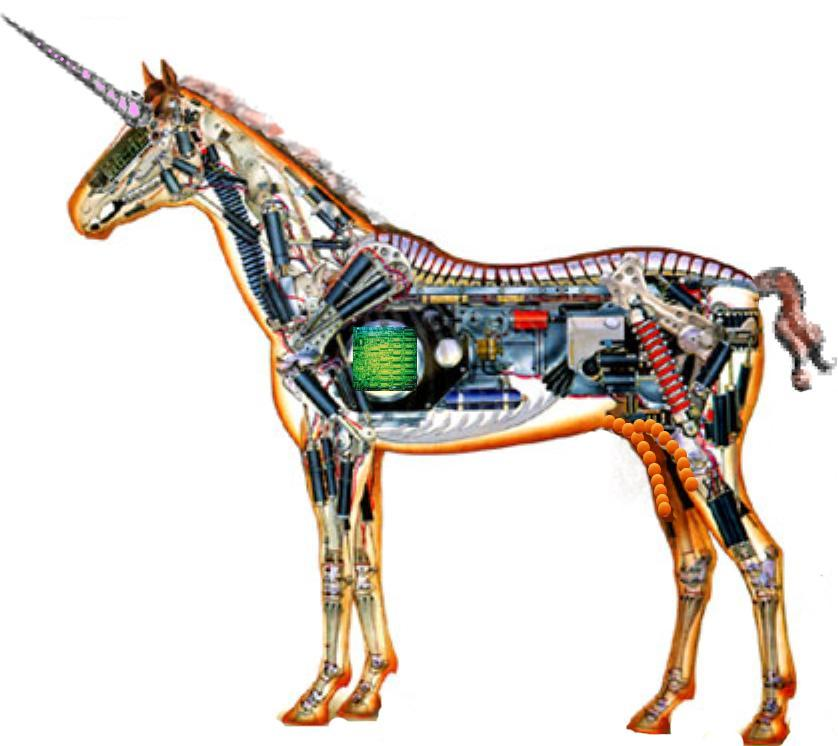
\includegraphics[width=5.9992in,height=5.3402in]{ib-img/ib-img001.jpg}
\end{center}
{\selectlanguage{english}\color{black}
\bfseries\Huge
The \vspace{0.05in}

\noindent \TitleFont
\begin{center}
\colorbox{blue}{\makebox[6.2in][r]{\parbox{6.2in}{\center\textcolor{white}{Implementation of\\ Icon and Unicon} \vspace{0.05in}}}}
\end{center}
}

\vspace{0.05in}

{\raggedleft\itshape\huge
a Compendium
\par}

\bigskip

{\raggedleft\LARGE
Clinton Jeffery and Don Ward, editors
\par}

\clearpage\setcounter{page}{1}\pagestyle{UnnumberedKonvertFolgeii}
\parbox{1in}{}

\clearpage

\bigskip
\bigskip
\bigskip

{\centering\bfseries\Huge
The Implementation\\
of Icon and Unicon
\par}

\bigskip
\bigskip
\bigskip
\bigskip
\bigskip
\bigskip
\bigskip

{\raggedleft\bfseries\Large
Ralph and Madge T. Griswold
\par
Kenneth W. Walker
\par
Clinton L. Jeffery 
\par}

\bigskip
\bigskip
\bigskip

\clearpage\setcounter{page}{1}\pagestyle{KonvertFolgeii}
\frontmatter
\bigskip
\bigskip
\noindent Copyright {\textcopyright} 2017 Clinton Jeffery


\noindent Permission is granted to copy, distribute and/or modify this
document under the terms of the GNU Free Documentation License,
Version 1.2 or any later version published by the Free Software
Foundation; with no Invariant Sections, no Front-Cover Texts, and no
Back-Cover Texts. A copy of the license is included in the section
entitled {\textquotedbl}GNU Free Documentation License{\textquotedbl}.


Portions of this document ({\textquotedbl}The Implementation of the
Icon Programming Language{\textquotedbl}) are in the public domain and
not subject to the above copyright or license. Other portions of this
document ({\textquotedbl}An Optimizing Compiler for
Icon{\textquotedbl}) are copyrighted by Kenneth Walker and appear in
edited form in this document with the express permission of the
author.


\bigskip
\raggedbottom

\noindent This is a draft manuscript dated \today.

\noindent Send comments and errata to
\href{mailto:jeffery@cs.uidaho.edu}{jeffery@cs.uidaho.edu}.

\bigskip

\noindent This document was prepared using \LaTeX. Special thanks to Don Ward
for assistance with the conversion to \LaTeX.

\setcounter{tocdepth}{3}
\tableofcontents
\section[Preface to the 2nd Edition]{Preface to the
2\textsuperscript{nd} Edition}

This book will raise your level of skill at computer programming,
regardless of whether you are presently a novice or expert. The field
of programming languages is still in its infancy, and dramatic advances
will be made every decade or two until mankind has had enough time to
think about the problems and principles that go into this exciting area
of computing. The Unicon language described in this book is such an
advance, incorporating many elegant ideas not yet found in most
contemporary languages.

Unicon is an object-oriented, goal-directed programming language based
on the Icon programming language. Unicon can be pronounced however you
wish; we pronounce it variably depending on mood, whim, or situation;
most frequently it either (a) rhymes with
{\textquotedbl}lexicon{\textquotedbl}, or (b) is pronounced as if it
stands for {\textquotedbl}un-Icon{\textquotedbl}.

For Icon programmers this work serves as a {\textquotedbl}companion
book{\textquotedbl} that documents material such as the Icon Program
Library, a valuable resource that is underutilized.
Don{\textquotesingle}t be surprised by language changes: the book
presents many new facilities that were added to Icon to make Unicon and
gives examples from new application areas to which Unicon is well
suited. For people new to Icon and Unicon, this book is an exciting
guide to a powerful language.

It is with sweet irony that we call this book the 2\textsuperscript{nd}
Edition, since the first edition was never formally published but
instead existed solely as an online document, although laser-printed
hard copies could be requested. A lot has happened to Unicon since the
first edition of this book, which culminated in 2004. This
{\textquotedblleft}2\textsuperscript{nd} Edition{\textquotedblright}
catches readers up with things like concurrent threads and vastly
improved 3D graphics facilities. Along the way, the games chapter and
parts of the internet programming chapter got spun off into a separate
work, the so-called \textit{Manual of Puissant Skill at Game
Programming}. 

\subsection{Organization of This Book}

This book consists of four parts. The first part, Chapters 1-8, presents
the core of the Unicon language, much of which comes from Icon. These
early chapters start with simple expressions, progress through data
structures and string processing, and include advanced programming
topics and the input/output capabilities of Unicon{\textquotesingle}s
portable system interface. Part two, in Chapters 9-12, describes
object-oriented development as a whole and presents
Unicon{\textquotesingle}s object-oriented facilities in the context of
object-oriented design. Object-oriented programming in Unicon
corresponds closely to object-oriented design diagrams in the Unified
Modeling Language, UML. Some of the most interesting parts of the book
are in part three; Chapters 13-18 provide example programs that use
Unicon in a wide range of application areas. Part four consists of
essential reference material presented in several Appendixes.

\subsection{Acknowledgments}

Thanks to the Icon Project for creating a most excellent language.
Thanks especially to those unsung heroes, the university students and
Internet volunteers who implemented the language and its
program library over a period of many years. Icon contributors can be
divided into epochs. In the epoch leading up to the first edition of
this book, we were inspired by
contributions from Gregg Townsend, Darren Merrill, Mary Cameron, Jon
Lipp, Anthony Jones, Richard Hatch, Federico Balbi, Todd Proebsting,
Steve Lumos and Naomi Martinez.  In the epoch since the first edition
of this book, the Unicon Project owes a debt of gratitude to Ziad al
Sharif, Hani bani Salameh, Jafar Al Gharaibeh, Mike Wilder, and Sudarshan
Gaikaiwari.

The most impressive contributors are those whose influence on Icon has
spanned across epochs, such as Ralph Griswold, Steve Wampler, Bob
Alexander, and Ken Walker. We revere you folks! Steve Wampler deserves
extra thanks for serving as the technical reviewer for this book.

This manuscript received critical improvements and corrections from many
additional technical reviewers, including Phillip Thomas, David A.
Gamey, Craig S. Kaplan, David Feustel, David Slate, Kostas Oikonomou,
Frank Lhota, Art Eschenlauer, Wendell Turner, Dennis Darland, and Nolan
Clayton.

The authors wish to acknowledge generous support from the National
Library of Medicine that enabled the development of the database
facilities. This work was also supported in part by the National
Science Foundation under grants CDA-9633299, \ EIA-0220590 and
EIA-9810732, and the Alliance for Minority Participation.

Clinton Jeffery

Shamim Mohamed

Ray Pereda

Robert Parlett


\mainmatter
\section{Introduction}

Software development requires thinking about several
dimensions simultaneously. For large programs, writing the actual
computer instructions is not as difficult as figuring out the
details of what the computer is supposed to do. After analyzing what is
needed, program design brings together the data structures, algorithms,
objects, and interactions that accomplish the required tasks. Despite
the importance of analysis and design, programming is still the central
act of software development for several reasons. The weak form of the
\index{Sapir-Whorf}Sapir-Whorf hypothesis suggests that the programming
language we use steers and guides the way we think about software, so
it affects our designs. Software designs are mathematical theorems,
while programs are proofs that test those designs. As in other
branches of mathematics, the proofs reign supreme. In addition, a
correct design can be foiled by an inferior implementation.

This book is a guide and reference for an exciting
programming language called Unicon that has something to offer both
computer scientists as well as casual programmers. You
will find explanations of fundamental principles, unique language
idioms, and advanced concepts and examples. Unicon exists within the
broader context of software development, so the book also covers
software engineering fundamentals. Writing a correct, working
program is the central task of software engineering. This does not
happen automatically as a result of the software design process. Make
no mistake: if you program very much, the programming language you use
is of vital importance. If it weren{\textquotesingle}t, we would still
be programming in machine language.

\subsection{Prototyping and the Spiral Model of Development}

A software \index{prototype}prototype is a working subset of a software
system. Prototypes help check software designs and user
interfaces, demonstrate key features to customers, or prove the
feasibility of a proposed solution. A prototype may generate
customer feedback on missing functionality, provide insight on how to
improve the design, lead to a decision about whether to go ahead with a
project or not, or form a starting point for the algorithms and data
structures that will go into the final product. Prototyping is done
early in the software development process. It fits naturally into the
\index{spiral model}\textit{spiral model} of development proposed by
\index{Boehm, Barry}Barry Boehm (1988). Figure I-1 shows the spiral
model; time is measured by the distance from the center. Analysis,
design, coding, and evaluation are repeated to produce a better product
with each iteration. {\textquotedbl}Prototyping{\textquotedbl} is the
act of coding during those iterations when the software is not yet
fully specified or the program does not yet remotely implement the
required functionality.

\begin{center}
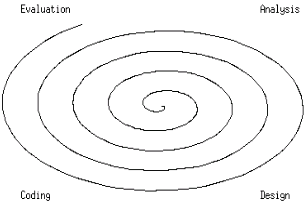
\includegraphics[width=2.5402in,height=1.6799in]{ub-img/ub-img4.png}
\end{center}

{\sffamily\bfseries Figure I-1}
{\sffamily The Spiral Model of Software Development}

\bigskip

\textit{Tight} spirals are better than loose spirals. The more powerful
the prototyping tools, the less time and money spent in early
iterations of development. This translates into either faster
time to market, or a higher quality product. Some prototypes are thrown
away once they have served the purpose of clarifying requirements or
demonstrating some technique. This is OK, but in the spiral model some
prototypes are gradually enhanced until they become the final
production system.

\subsection{Icon: a Very High Level Language for Applications}

Icon is a \index{very high-level language}programming language developed
at the University of Arizona. Icon generalizes its developers' experience
creating an earlier language, \index{SNOBOL4}SNOBOL4. Icon
embodies seminal research ideas, but it is also more fun and
easier to program than other languages.  Most very high-level
languages revel in cryptic syntax, while Icon
is not just more powerful, but often more
\textit{readable} than its competitors. This
gain in expressive power without losing readability is an
addicting result of Icon{\textquotesingle}s elegant design.

The current Arizona Icon, version 9.5, is described in
\textit{The Icon Programming Language}, \textit{3rd edition} by Ralph
and Madge Griswold (1996). Its reference implementation is a
virtual machine interpreter. Icon evolved through many releases
over two decades and is far more capable than it was originally. It is
apparently a finished work.

\subsection{Enter Unicon: More Icon than Icon}

The name Unicon\textbf{\textsuperscript{ }}refers to the descendant of
Icon described in this book and distributed from unicon.org. Unicon is
Icon with portable, platform-independent access to hardware and
software features that have become ubiquitous in modern
applications development, such as objects, networks, and databases.
Unicon is created from the same public domain source code that Arizona
Icon uses, so it has a high degree of compatibility. We were not
free to call it version 10 of the Icon
language, since it was not produced or endorsed by the Icon Project at
the University of Arizona.

Just as the name Unicon frees the Icon Project of all responsibility for
our efforts, it frees us from the requirement of backward
compatibility. While Unicon is almost entirely backward compatible
with Icon, dropping full
compatibility allows us to clear out some dead wood and more
importantly, to make some improvements in the operators that will
benefit everyone at the expense of...no one but the compatibility
police.
This book covers the features of Icon and Unicon together. A
compatibility check list and description of the differences
between Icon and Unicon are given in Appendix D.

\subsection{The Programming Languages Food Chain}

It is interesting to compare Icon and Unicon with the competition.
Mainstream programming languages
such as C, C++, and \index{Java}Java, like the assembler languages that
was mainstream before them, are ideal tools
for writing all sorts of programs, so long as vast amounts of
programmer time are available. Throwing more programmers at a big
project does not work well, and programmers are getting more expensive
while computing
resources continue to become cheaper. These pressures
inexorably lead to the use of higher-level languages and the
development of better design and development methods. Such human
changes are incredibly slow compared to technological changes, but they
are visibly occurring nevertheless. Today, the most
productive programmers are using extra CPU cycles and memory
to reduce the time it takes to develop useful programs.

There is a subcategory of mainstream languages, marketed as \index{rapid
application development}\textit{rapid application development}
languages, whose stated goals seem to address this phenomenon.
Languages such as \index{Visual Basic}Visual Basic or
\index{PowerBuilder}PowerBuilder provide
graphical interface builders and integrated database connectivity,
giving productivity increases in the domain of data entry and
presentation. The value added in these products are in their
programming environments, not their languages. The \index{integrated
development environment}integrated development environments and tools
provided with these languages are to be acclaimed and emulated, but
they do not provide productivity gains that are equally relevant to all
application domains. They are only a partial solution to the needs of
complex applications.

Icon is designed to be easier and faster to program than mainstream
languages. The value it adds is in the expressive power of the language
itself, in the category of very high level languages
that includes \index{Lisp}Lisp,
\index{APL}APL, \index{Smalltalk}Smalltalk, \index{REXX}REXX,
\index{Perl}Perl, \index{Tcl}Tcl, \index{Python}Python, and
\index{Ruby}Ruby; there are
many others. Very high-level languages can be subdivided into
\index{scripting languages}scripting languages and applications
languages. Scripting languages often glue programs
together from disparate sources. They are typically strong in areas
such as multilingual interfacing and file system interactions, while
suffering from weaker expression semantics, typing, scope rules, and
control structures than their applications-oriented cousins.
Applications languages typically originate within a particular
application domain and support that domain with special syntax, control
structures, and data types. Since scripting \textit{is} an application
domain, scripting languages are just one prominent
subcategory of very high-level languages.

Icon is an applications language with roots in text
processing and linguistics. Icon programs tend to be more readable than
similar programs written in other very high-level languages, making
Icon well-suited to the aims of \index{literate
programming}\textit{literate programming}. For example, Icon was used
to implement Norman Ramsey{\textquotesingle}s literate
programming tool \texttt{noweb} (Ramsey, 1994). Literate programming is
the practice of writing programs and their supporting textual
description together in a single document.

Unicon makes the core contributions of Icon useful
for a broader range of applications. This book's many
examples illustrate the range of tasks for which Unicon is well
suited, and these examples are the evidence in
support of Unicon's existence.
Consider using Unicon when one or more of the following conditions are
true. The more conditions that are true, the more you will
benefit from Unicon.

\begin{itemize} \itemsep0pt
\item Programmer time must be minimized.
\item Maintainable, concise source code is desired.
\item The program includes complex data structures or experimental
algorithms.
\item The program involves a mixture of text processing and analysis, custom
graphics, data manipulation, network or file system operations.
\item The program must run on several operating systems and have a
nearly identical graphical user interface with little or no source code
differences.
\end{itemize}

Unicon is not the last word in programming. You probably should not use
Unicon if your program has one or more of the following requirements:

\begin{itemize} \itemsep0pt
\item The fastest possible performance is needed.
\item The program has hard real-time constraints.
\item The program must perform low-level or platform-specific
interactions with the hardware or operating system.
\end{itemize}

Programming languages play a key role in software development.
The Unicon language is a very high level
\index{object-oriented programming}object-oriented language
with a unique combination of expressive power and scalable rapid
development. In this book, many examples from a wide range
of application areas demonstrate how to apply and combine Unicon's
language constructs to solve real-world problems.
It is time to move past the introductions. Prepare to be spoiled by
this language. You may have the same feelings that
Europeans felt when they gave up using Roman numerals and
switched to the Hindu-Arabic number system. {\textquotedbl}This
multiplication stuff isn{\textquotesingle}t that hard
anymore!{\textquotedbl} 


\part{The Implementation of the Icon Programming Language}

\chapter{Introduction}

\textsc{Perspective}: The implementation of complex software systems
is a fascinating subject --- and an important one. Its theoretical and
practical aspects occupy the attention and energy of many persons, and
it consumes vast amounts of computational resources. In general terms,
it is a broad subject ranging from operating systems to programming
languages to data-base systems to real-time control systems, and so
on.


Past work in these areas has resulted in an increasingly better
understanding of implementation techniques, more sophisticated and
efficient systems, and tools for automating various aspects of
software production. Despite these advances, the implementation of
complex software systems remains challenging and exciting. The
problems are difficult, and every advance in the state of the art
brings new and more difficult problems within reach.


Part I of this book addresses a very small portion of the problem of
implementing complex software systems{}---the implementation of a very
high-level programming language that is oriented toward the
manipulation of structures and strings of characters.


In a narrow sense, this book describes an implementation of a specific
programming language, Icon. In a broader sense, it deals with a
language-design philosophy, an approach to implementation, and
techniques that apply to the implementation of many programming
languages as well as related types of software systems.


The focus of this book is the implementation of programming language
features that are at a high conceptual level{}---features that are
easy for human beings to use as opposed to features that fit
comfortably on conventional computer architectures. The orientation of
the implementation is generality and flexibility, rather than maximum
efficiency of execution. The problem domain is strings and structures
rather than numbers. It is these aspects that set the implementation
of Icon apart from more conventional programming-language
implementations.

\section{Implementing Programming Languages}

In conventional programming languages, most of the operations that are
performed when a program is executed can be determined, statically, by
examining the text of the program. In addition, the operations of most
programming languages have a fairly close correspondence to the
architectural characteristics of the computers on which they are
implemented.  When these conditions are met, source-code constructs
can be mapped directly into machine instructions for the computer on
which they are to be executed. The term \textit{compilation} is used
for this translation process, and most persons think of the
implementation of a programming language in terms of a compiler.

Writing a compiler is a complex and difficult task that requires
specialized training, and the subject of compilation has been studied
extensively (Waite and Goos, 1984; Aho, Lam, Sethi and Ullman
2006). Most of the issues of data representation and code generation
are comparatively well understood, and there are now many tools for
automating portions of the compiler-writing task (Lesk 1975, Johnson
1975).


In addition to the compiler proper, an implementation of a programming
language usually includes a run-time component that contains
subroutines for performing computations that are too complex to
compile in-line, such as input, output, and mathematical functions.


Some programming languages have features whose meanings cannot be
determined statically from the text of a source-language program, but
which may change during program execution. Such features include
changes in the meaning of functions during execution, the creation of
new data types at run time, and self-modifying programs. Some
programming languages also have features, such as pattern matching,
that do not have correspondences in the architecture of conventional
computers. In such cases, a compiler cannot translate the source
program directly into executable code.  Very high-level operations,
such as pattern matching, and features like automatic storage
management significantly increase the importance and complexity of the
run-time system. For languages with these characteristics-{}-languages
such as APL, LISP, SNOBOL4, SETL, Prolog, and Icon-much of the
substance of the implementation is in the run-time system rather than
in translation done by a compiler. While compiler writing is
relatively well understood, run-time systems for most programming
languages with dynamic features and very high-level operations are
not.


Programming languages with dynamic aspects and novel features are
likely to become more important rather than less important. Different
problems benefit from different linguistic mechanisms. New
applications place different values on speed of execution, memory
requirements, quick solutions, programmer time and talent, and so
forth. For these reasons, programming languages continue to
proliferate. New programming languages, by their nature, introduce new
features.


All of this creates difficulties for the implementer. Less of the
effort involved in implementations for new languages lies in the
comparatively familiar domain of compilation and more lies in new and
unexplored areas, such as pattern matching and novel
expression-evaluation mechanisms.

The programming languages that are the most challenging to implement
are also those that differ most from each other.  Nevertheless, there
are underlying principles and techniques that are generally
applicable, and existing implementations contain many ideas that can
be used or extended in new implementations.

\section{The Background for Icon}

Before describing the Icon programming language and its
implementation, some historical context is needed, since both the
language and its implementation are strongly influenced by earlier
work.

Icon has its roots in a series of programming languages that bear the
name SNOBOL. The first SNOBOL language was conceived and implemented
in the early 1960s at Bell Telephone Laboratories in response to the
need for a programming tool for manipulating strings of characters at
a high conceptual level (Farber, Griswold, and Polonsky 1964). It
emphasized ease of programming at the expense of efficiency of
execution; the programmer was considered to be a more valuable
resource than the computer.

This rather primitive language proved to be popular, and it was
followed by successively more sophisticated languages: SNOBOL2,
SNOBOL3 (Farber, Griswold, and Polonsky 1966), and finally SNOBOL4
(Griswold, Poage, and Polonsky 1971).  Throughout the development of
these languages, the design emphasis was on ease of programming rather
than on ease of implementation (Griswold 1981). Potentially valuable
features were not discarded because they might be inefficient or
difficult to implement. The aggressive pursuit of this philosophy led
to unusual language features and to challenging implementation
problems.

SNOBOL4 still is in wide use. Considering its early origins, some of
its facilities are remarkably advanced. It features a pattern-matching
facility with backtracking control structures that effectively
constitutes a sublanguage. SNOBOL4 also has a variety of data
structures, including tables with associative lookup. Functions and
operators can be defined and redefined during program execution.
Identifiers can be created at run-time, and a program can even modify
itself by means of run-time compilation.

Needless to say, SNOBOL4 is a difficult language to implement, and
most of the conventional compilation techniques have little
applicability to it. Its initial implementation was, nonetheless,
sufficiently successful to make SNOBOL4 widely available on machines
ranging from large mainframes to personal computers (Griswold
1972). Subsequent implementations introduced a variety of clever
techniques and fast, compact implementations (Santos 1971; Gimpel
1972a; Dewar and McCann 1977). The lesson here is that the design of
programming languages should not be overly inhibited by perceived
implementation problems, since new implementation techniques often can
be devised to solve such problems effectively and efficiently.

It is worth noting that the original implementation of SNOBOL4 was
carried out concomitantly with language design. The implementation was
sufficiently flexible to serve as a research tool in which
experimental language features could be incorporated easily and tested
before they were given a permanent place in the language.

Work on the SNOBOL languages continued at the University of Arizona in
the early 1970s. In 1975, a new language, called SL5
({\textquotedbl}SNOBOL Language 5{\textquotedbl}), was developed to
allow experimentation with a wider variety of programming-language
constructs, especially a sophisticated procedure mechanism (Griswold
and Hanson, 1977; Hanson and Griswold 1978). SL5 extended earlier work
in pattern matching, but pattern matching remained essentially a
sublanguage with its own control structures, separate from the rest of
the language.

The inspiration for Icon came in 1976 with a realization that the
control structures that were so useful in pattern matching could be
integrated with conventional computational control structures to yield
a more coherent and powerful programming language.


The first implementation of Icon (Griswold and Hanson 1979) was
written in Ratfor, a preprocessor for Fortran that supports structured
programming features (Kernighan 1975). Portability was a central
concern in this implementation.  The implementation of Icon described
in this book is a successor to that first implementation. It borrows
much from earlier implementations of SNOBOL4, SL5, and the Ratfor
implementation of Icon. As such, it is a distillation and refinement
of implementation techniques that have been developed over a period of
more than twenty years.


\bigskip

\chapter{Icon Language Overview}

\textsc{Perspective}: The implementer of a programming language needs
a considerably different understanding of the language from the
persons who are going to use it. An implementer must have a deep
understanding of the relationships that exist among various aspects of
the language and a precise knowledge of what each operation
means. Special cases and details often are of particular importance to
the implementer. Users of a language, on the other hand, must know how
to use features to accomplish desired results. They often can get by
with a superficial knowledge of the language, and they often can use
it effectively even if some aspects of the language are
misunderstood. Users can ignore parts of the language that they do not
need. Idiosyncrasies that plague the implementer may never be
encountered by users.  Conversely, a detail the implementer overlooks
may bedevil users. Furthermore, the implementer may also need to
anticipate ways in which users may apply some language features in
inefficient and inappropriate ways.

Part I of this book is about the implementation of Version 6
(discussion partially updated to Version 9) of Icon. The description
that follows concentrates on aspects of the language that are needed
to understand its implementation. Where there are several similar
operations or where the operations are similar to those in well-known
programming languages, only representative cases or highlights are
given. A complete description of Icon for the user is contained in
Griswold and Griswold (1997).

Icon is an unusual programming language, and its unusual features are
what make its implementation challenging and interesting. The
interesting features are semantic, not syntactic; they are part of
what the language can do, not part of its appearance. Syntactic
matters and the way they are handled in the implementation are of
little interest here.  The description that follows indicates syntax
mostly by example.

This chapter is divided into two major parts. The first part describes
the essential aspects of Icon. The second part discusses those aspects
of Icon that present the most difficult implementation problems and
that affect the nature of the implementation in the most significant
ways.

\section[2.1 The Icon Programming Language]{2.1 The Icon Programming Language}

Icon is conventional in many respects. It is an imperative, procedural
language with variables, operations, functions, and conventional data
types. Its novel aspects lie in its emphasis on the manipulation of
strings and structures and in its expression-evaluation
mechanism. While much of the execution of an Icon program has an
imperative flavor, there also are aspects of logic programming.

There are no type declarations in Icon. Instead, variables can have
any type of value. Structures may be heterogeneous, with different
elements having values of different types. Type checking is performed
during program execution, and automatic type conversion is
provided. Several operations are polymorphic, performing different
operations depending on the types of their arguments.

Strings and structures are created during program execution, instead
of being declared and allocated during compilation.  Structures have
pointer semantics; a structure value is a pointer to an object.
Storage management is automatic. Memory is allocated as required, and
garbage collection is performed when necessary. Except for the
practical considerations of computer architecture and the amount of
available memory, there are no limitations on the sizes of objects.

An Icon program consists of a series of declarations for procedures,
records, and global identifiers. Icon has no block structure. Scoping
is static: identifiers either are global or are local to procedures.

Icon is an expression-based language with reserved-word syntax. It
resembles C in appearance, for example (Kernighan and Ritchie 1978).

{\sffamily\bfseries
2.1.1 Data Types}

Icon has many types of data --- including several that are not found in
most programming languages. In addition to the usual integers and real
(floating-point) numbers, there are strings of characters and sets of
characters (csets). There is no character data type, and strings of
characters are data objects in their own right, not arrays of
characters.

There are four structure data types that comprise aggregates of
values: lists, sets, tables, and records. Lists provide positional
access (like vectors), but they also can be manipulated like stacks
and queues. Sets are unordered collections of values on which the
usual set operations can be performed. Tables can be subscripted with
any kind of value and provide an associative-access mechanism. Records
are aggregates of values that can be referenced by name.  Record types
also add to the built-in type repertoire of Icon.

The null value serves a special purpose; all variables have the null value initially. The null value is illegal in most
computational contexts, but it serves to indicate default values in a number of situations. The keyword \&null produces
the null value.

A source-language file is a data value that provides an interface
between the program and a data file in the environment in which the
program executes.

Procedures also are data values --- {\textquotedbl}first-class data
objects{\textquotedbl} in LISP parlance.  Procedures can be assigned
to variables, transmitted to and returned from functions, and so
forth. There is no method for creating procedures during program
execution, however.

Finally, there is a co-expression data type. Co-expressions are the
expression-level analog of coroutines. The importance of
co-expressions is derived from Icon's expression-evaluation mechanism.

Icon has various operations on different types of data. Some
operations are polymorphic and accept arguments of different
types. For example, type(x) produces a string corresponding to the
type of x. Similarly, copy(x) produces a copy of x, regardless of its
type. Other operations only apply to certain types. An example is:

\iconcode{
\> *x
}


\noindent which produces the size of x, where the value of x may be a
string, a structure, and so on. Another example is ?x, which produces
a randomly selected integer between 1 and x, if x is an integer, but a
randomly selected one-character substring of x if x is a string, and
so on. In other cases, different operations for similar kinds of
computations are syntactically distinguished. For example,

{\ttfamily\mdseries
\ \ \ i = j}

\noindent compares the numeric values of i and j, while

{\ttfamily\mdseries
\ \ \ s1 == s2}


\noindent compares the string values of s1 and s2. There is also a
general comparison operation that determines whether any two objects
are the same:

{\ttfamily\mdseries
\ \ x1 === x2}

As mentioned previously, any kind of value can be assigned to any
variable. For example, x might have an integer value at one time and a
string value at another:

{\ttfamily\mdseries
\ \ \ x := 3 \\
\ \ \ ... \\
\ \ \ x := {\textquotedbl}hello{\textquotedbl}}

Type checking is performed during program execution. For example, in

{\ttfamily\mdseries
\ \ \ i := x + 1}

the value of x is checked to be sure that it is numeric. If it is not
numeric, an attempt is made to convert it to a numeric type. If the
conversion cannot be performed, program execution is terminated with
an error message.

Various conversions are supported. For example, a number always can be
converted to a string. Thus,

{\ttfamily\mdseries
\ \ \ write(*s)}

\noindent automatically converts the integer returned by *s to a
string for the purpose of output.

There also are explicit type-conversion functions. For example,

{\ttfamily\mdseries
\ \ \ s1 := string(*s2)}

\noindent assigns to s1 a string corresponding to the size of s2.

A string can be converted to a number if it has the syntax of a number. Thus,

{\ttfamily\mdseries
\ \ \ i := i + {\textquotedbl}20{\textquotedbl}}

\noindent produces the same result as

{\ttfamily\mdseries
\ \ \ i := i + 20}


Augmented assignments are provided for binary operations such as the
previous one, where assignment is made to the same variable that
appears as the left argument of the operation. Therefore, the previous
expression can be written more concisely as

{\ttfamily\mdseries
\ \ \ i +:= 20}


Icon also has the concept of a numeric type, which can be either an
integer or a real (floating-point) number.

{\sffamily\bfseries
2.1.2 Expression Evaluation}


In most programming languages --- Algol, Pascal, PL/I, and C, for
example --- the evaluation of an expression always produces exactly
one result. In Icon, the evaluation of an expression may produce a
single result, it may produce no result at all, or it may produce a
sequence of results.

\textbf{Success and Failure}. Conventional operations in Icon
produce one result, as they do in most programming languages. For
example,

{\ttfamily\mdseries
\ \ \ i + j}

\noindent produces a single result, the sum of the values of i and
j. However, a comparison operation such as

{\ttfamily\mdseries
\ \ \ i {\textgreater} j}

\noindent produces a result (the value of j) if the value of i is
greater than the value of j but does not produce a result if the value
of i is not greater than j.

An expression that does not produce a result is said to \textit{fail},
while an expression that produces a result is said to
\textit{succeed}. Success and failure are used in several control
structures to control program flow. For example,

{\ttfamily\mdseries
\ \ \ if i {\textgreater} j then write(i) else write(j)}

\noindent writes the maximum of i and j. Note that comparison
operations do not produce Boolean values and that Boolean values are
not used to drive control structures. Indeed, Icon has no Boolean
type.

Generally speaking, an operation that cannot perform a computation
does not produce a result, and hence it fails. For example,
type-conversion functions fail if the conversion cannot be
performed. An example is numeric(x), which converts x to a numeric
value if possible, but fails if the conversion cannot be
performed. Failure of an expression to produce a result does not
indicate an error. Instead, failure indicates that a result does not
exist. An example is provided by the function find(s1, s2), which
produces the position of s1 as a substring of s2 but fails if s1 does
not occur in s2.  For example,

{\ttfamily\mdseries
\ \ \ find({\textquotedbl}it{\textquotedbl}, {\textquotedbl}They sit like bumps on a log.{\textquotedbl})}

\noindent
produces the value 7 (positions in strings are counted starting at 1). However,

\iconcode{
\> find("at", "They sit like bumps on a log.")
}

\noindent
does not produce a result. Similarly, read(f) produces the next line from the file f but fails when the end of the file
is reached.


Failure provides a natural way to control loops. For example,

\iconcode{
\>  while line := read(f) do\\
\> \>  write(line)
}

\noindent
writes the lines from the file f until an end of file causes read to fail, which terminates the loop.


Another use of success and failure is illustrated by the operation

{\ttfamily\mdseries
\ \ \ {\textbackslash}expr}


which fails if \textit{expr }is null-valued but produces the result of \textit{expr }otherwise. Since variables have the
null value initially, this operation may be used to determine whether a value has been assigned to an identifier, as
in

{\ttfamily\mdseries
\ \ \ if {\textbackslash}x then write(x) else write({\textquotedbl}x is null{\textquotedbl})}


If an expression that is enclosed in another expression does not produce a result, there is no value for the enclosing
expression, it cannot perform a computation, and it also produces no result. For example. In

{\ttfamily\mdseries
\ \ \ write(find({\textquotedbl}at{\textquotedbl}, {\textquotedbl}They sit like bumps on a log.{\textquotedbl}))}

\noindent the evaluation of find fails, there is no argument for write, and no value is written.

Similarly, in

{\ttfamily\mdseries
\ \ \ i := find({\textquotedbl}at{\textquotedbl}, {\textquotedbl}They sit like bumps on a log.{\textquotedbl})}

\noindent the assignment is not performed and the value of i is not changed.


This {\textquotedbl}inheritance{\textquotedbl} of failure allows computations to be expressed concisely. For example,

{\ttfamily\mdseries
\ \ \ while write(read(f))}

\noindent writes the lines from the file f just as the previous loop
(the do clause in while-do is optional).

The expression

{\ttfamily\mdseries
\ \ \ not \textit{expr}}

\noindent inverts success and failure. It fails if \textit{expr}
succeeds, but it succeeds, producing the null value, if \textit{expr}
fails.

Some expressions produce variables, while others only produce
values. For example,

{\ttfamily\mdseries
\ \ \ i + j}

\noindent produces a value, while

{\ttfamily\mdseries
\ \ \ i := 10}

\noindent produces its left-argument variable. The term
\textit{result} is used to refer to a value or a variable. The term
\textit{outcome }is used to refer to the consequences of evaluating an
expression --- either its result or failure.

\textbf{Loops}. \ There are several looping control structures in Icon in addition to while-do. For example,

{\ttfamily\mdseries
\ \ \ until \textit{expr1 }do \textit{expr2}}

\noindent evaluates \textit{expr2} repeatedly until \textit{expr1}
succeeds. The control structure

{\ttfamily\mdseries
\ \ \ repeat expr}

\noindent simply evaluates \textit{expr} repeatedly, regardless of
whether it succeeds or fails.

A loop itself produces no result if it completes, and hence it fails
if used in a conditional context. That is, when

{\ttfamily\mdseries
\ \ \ while \textit{expr1 }do \textit{expr2}}

\noindent terminates, its outcome is failure. This failure ordinarily
goes unnoticed, since loops usually are not used as arguments of other
expressions.

The control structure

{\ttfamily\mdseries
\ \ \ break \textit{expr}}

\noindent causes the immediate termination of the evaluation of the
loop in which it appears, and control is transferred to the point
immediately after the loop. The outcome of the loop in this case is
the outcome of \textit{expr}. If \textit{expr} is omitted, it defaults
to the null value.

An example of the use of break is:

{\ttfamily\mdseries
\ \ \ while line := read(f) do\newline
 \ \ \ \ \ if line == {\textquotedbl}end{\textquotedbl} then break\newline
 \ \ \ \ \ else write(line)}

Evaluation of the loop terminates if read fails or if the file f
contains a line consisting of {\textquotedbl}end{\textquotedbl}.

The expression next causes transfer to the beginning of the loop in
which it occurs. For example,

\iconcode {
\> while line := read(f) do \\
\> \> if line == "comment" then next \\
\> \> else write(line)
}

\noindent does not write the lines of f that consist of
{\textquotedbl}comment{\textquotedbl}.

The break and next expressions can occur only in loops, and they apply
to the innermost loop in which they appear. The argument of break can
be a break or next expression, however, so that, for example,

{\ttfamily\mdseries
\ \ \ break break next}

\noindent breaks out of two levels of loops and transfers control to
the beginning of the loop in which they occur.


\textbf{Case Expressions}. The case expression provides a way of
selecting one of several expressions to evaluate based on the value of
a control expression, rather than its success or failure. The case
expression has the form

{\ttfamily\mdseries
\ \ \ case \textit{expr} of \{\\
\ \ \ \ \ \ case clauses \\
\ \ \ \ \ \ ... \\
\ \ \ \ \ \ \}}

The value of \textit{expr }is used to select one of the case
clauses. A case clause has the form

{\ttfamily\mdseries
\textit{\ \ \ expr1 }: \textit{expr2}}

\noindent where the value of \textit{expr} is compared to the value of
\textit{expr1}, and \textit{expr2} is evaluated if the comparison
succeeds. There is also a default case clause, which has the form

{\ttfamily\mdseries
\ \ \ default: expr3}


If no other case clause is selected, expr3 in the default clause is
evaluated. An example is

{\ttfamily\mdseries
\ \ \ case line := read(f) of \{\newline
 \ \ \ \ \ {\textquotedbl}end{\textquotedbl}:\ \ \ \ write({\textquotedbl}*** end ***{\textquotedbl})\newline
 \ \ \ \ \ {\textquotedbl}comment{\textquotedbl}:\ \ write({\textquotedbl}*** comment ***{\textquotedbl})\newline
 \ \ \ \ \ default:\ \ write(line)\newline
 \ \ \ \ \ \}}


If the evaluation of the control clause fails, as for an end of file in this example, the entire case expression fails.
Otherwise, the outcome of the case expression is the outcome of evaluating the selected expression.


\textbf{Generators}. As mentioned previously, an expression may
produce a sequence of results. This occurs in situations in which
there is more than one possible result of a computation. An example is

{\ttfamily\mdseries
\ \ \ find({\textquotedbl}e{\textquotedbl}, {\textquotedbl}They sit like bumps on a log.{\textquotedbl})}

\noindent in which both 3 and 13 are possible results.

While most programming languages produce only the first result in such
a situation, in Icon the two results are produced one after another if
the surrounding context requires both of them. Such expressions are
called \textit{generators} to emphasize their capability of producing
more than one result.

There are two contexts in which a generator can produce more than one
result: \textit{iteration} and \textit{goal-directed evaluation}.

Iteration is designated by the control structure

{\ttfamily\mdseries
\ \ \ every expr1 do expr2}

\noindent in which expr1 is repeatedly resumed to produce its
results. For each such result, expr2 is evaluated. For example,

{\ttfamily\mdseries
\ \ \ every i := find({\textquotedbl}e{\textquotedbl}, {\textquotedbl}They sit like bumps on a log.{\textquotedbl})
do\newline
 \ \ \ \ \ write(i)}

\noindent writes 3 and 13.

If the argument of an expression is a generator, the results produced
by the generator are provided to the enclosing expression{}---the
sequence of results is inherited. Consequently, the previous
expression can be written more compactly as

{\ttfamily\mdseries
\ \ \ every write(find({\textquotedbl}e{\textquotedbl}, {\textquotedbl}They sit like bumps on a log.{\textquotedbl}))}


Unlike iteration, which resumes a generator repeatedly to produce all
its results, goal-directed evaluation resumes a generator only as
necessary, in an attempt to cause an enclosing expression to
succeed. While iteration is explicit and occurs only where specified,
goal-directed evaluation is implicit and is an inherent aspect of
Icon's expression-evaluation mechanism.


Goal-directed evaluation is illustrated by

{\ttfamily\mdseries
\ \ \ if find({\textquotedbl}e{\textquotedbl}, {\textquotedbl}They sit like bumps on a log{\textquotedbl})
{\textgreater} 10\newline
 \ \ then write({\textquotedbl}found{\textquotedbl})}

The first result produced by \texttt{find()} is 3, and the comparison
operation fails. Because of goal-directed evaluation, find is
automatically resumed to produce another value. Since this value, 13,
is greater than 10, the comparison succeeds, and found is written. On
the other hand, in

{\ttfamily\mdseries
\ \ \ if find({\textquotedbl}e{\textquotedbl}, {\textquotedbl}They sit like bumps on a log.{\textquotedbl})
{\textgreater} 20\newline
 \ \ then write({\textquotedbl}found{\textquotedbl})}

\noindent the comparison fails for 3 and 13. When find is resumed
again, it does not produce another result, the control clause of
if-then fails, and nothing is written.

There are several expressions in Icon that are generators, including
string analysis functions that are similar in nature to find. Another
generator is

{\ttfamily\mdseries
\ \ \ i to j by k}

which generates the integers from \texttt{i} to \texttt{j} by
increments of \texttt{k}. If the \texttt{by} clause is omitted, the
increment defaults to one.

The operation \texttt{!x} is polymorphic, generating the elements of
\texttt{x} for various types. The meaning of
{\textquotedbl}element{\textquotedbl} depends on the type of
\texttt{x}. If \texttt{x} is a string, \texttt{!x} generates the
one-character substrings of \texttt{x}, so that
\texttt{!{\textquotedbl}hello{\textquotedbl}} generates
\texttt{{\textquotedbl}h{\textquotedbl}},
\texttt{{\textquotedbl}e{\textquotedbl}},
\texttt{{\textquotedbl}l{\textquotedbl}},
\texttt{{\textquotedbl}l{\textquotedbl}}, and
\texttt{{\textquotedbl}o{\textquotedbl}}. If \texttt{x} is a file,
\texttt{!x} generates the lines of the file, and so on.


\textbf{Generative Control Structures}. There are several control
structures related to generators. The \textit{alternation} control
structure,

{\ttfamily\mdseries
\ \ \ expr1 {\textbar} expr2}

\noindent
generates the results of expr1 followed by the results of expr2. For example,

{\ttfamily\mdseries
\ \ \ every write({\textquotedbl}hello{\textquotedbl} {\textbar} {\textquotedbl}howdy{\textquotedbl})}

\noindent writes two lines, hello and howdy.

Since alternation succeeds if either of its arguments succeeds, it can
be used to produce the effect of logical disjunction. An example is

{\ttfamily\mdseries
\ \ \ if (i {\textgreater} j) {\textbar} (j {\textgreater} k) then expr}

\noindent
which evaluates expr if i is greater than j or if j is greater than k.

Logical conjunction follows as a natural consequence of goal-directed
evaluation. The operation

{\ttfamily\mdseries
\textit{\ \ \ expr1 }\& \textit{expr2}}

\noindent is similar to other binary operations, such as
\textit{expr1} + \textit{expr2}, except that it performs no
computation. Instead, it produces the result of \textit{expr2},
provided that both
\textit{expr1} and \textit{expr2} succeed. For example,

{\ttfamily\mdseries
\ \ \ if (i {\textgreater} j) \& (j {\textgreater} k) then \textit{expr}}

\noindent
evaluates \textit{expr} only if i is greater than j and j is greater than k.

Repeated alternation,

{\ttfamily\mdseries
\ \ \ {\textbar}expr}

\noindent
generates the results of \textit{expr }repeatedly and is roughly equivalent to

{\ttfamily\mdseries
\textit{\ \ \ expr }{\textbar} \textit{expr }{\textbar} \textit{expr }{\textbar} ...}

However, if \textit{expr} fails, the repeated alternation control
structure stops generating results. For example,

{\ttfamily\mdseries
\ \ \ {\textbar}read(f)}

\noindent generates the lines from the file f (one line for each
repetition of the alternation) but stops when read(f) fails.

Note that a generator may be capable of producing an infinite number
of results. For example,

{\ttfamily\mdseries
\ \ \ {\textbar}(1 to 3)}

\noindent can produce 1, 2, 3, 1, 2, 3, 1, 2, 3,\ \ However, only as
many results as are required by context are actually produced. Thus,

{\ttfamily\mdseries
\ \ \ i := {\textbar} (1 to 3)}

\noindent only assigns the value 1 to i, since there is no context to
cause the repeated alternation control structure to be resumed for a
second result.

The \textit{limitation }control structure

{\ttfamily\mdseries
\textit{\ \ \ expr1 }{\textbackslash} \textit{expr2}}

\noindent
limits \textit{expr1 }to at most \textit{expr2 }results. Consequently,

{\ttfamily\mdseries
\ \ \ {\textbar} (1 to 3) {\textbackslash} 5}

is only capable of producing 1, 2, 3, 1, 2.

\textbf{The Order of Evaluation.} With the exception of the limitation
control structure, argument evaluation in Icon is strictly
left-to-right. The resumption of expressions to produce additional
results is in last-in, first-out order. The result is
{\textquotedbl}cross-product{\textquotedbl} generation of results in
expressions that contain several generators. For example,

{\ttfamily\mdseries
\ \ \ every write((10 to 30 by 10) + (1 to 3))}


\ writes\ \ 11, 12, 13, 21, 22, 23, 31, 32, 33.


\textbf{Control Backtracking}. Goal-directed evaluation results in
control backtracking to obtain additional results from expressions
that have previously produced results, as in

{\ttfamily\mdseries
\ \ \ if find({\textquotedbl}e{\textquotedbl}, {\textquotedbl}They sit like bumps on a log.{\textquotedbl})
{\textgreater} 10\newline
 \ \ then write({\textquotedbl}found{\textquotedbl})}

Control backtracking is limited by a number of syntactic
constructions. For example, in

{\ttfamily\mdseries
\ \ \ if \textit{expr1 }then \textit{expr2 }else \textit{expr3}}

\noindent if \textit{expr1} succeeds, but \textit{expr2} fails,
\textit{expr1} is not resumed for another result. (If it were, the
semantics of this control structure would not correspond to what
{\textquotedbl}if-then-else{\textquotedbl} suggests.)  Such an
expression is called a \textit{bounded expression}. The control
clauses of loops also are bounded, as are the expressions within
compound expressions:

{\ttfamily\mdseries
\ \ \ \{ \textit{expr}\textit{\TextSubscript{1}}\textit{; expr}\textit{\TextSubscript{2}}\textit{;
expr}\textit{\TextSubscript{3}}\textit{; }...; \textit{expr}\textit{\TextSubscript{n}}\textit{ }\}}

These expressions are evaluated in sequence, but once the evaluation
of one is complete (whether it succeeds or fails), and the evaluation
of another begins, there is no possibility of backtracking into the
preceding one. The last expression in a compound expression is not
bounded, however.

Except in such specific situations, expressions are not bounded. For
example, in

{\ttfamily\mdseries
\ \ \ if \textit{expr}\textit{\TextSubscript{1}}\textit{ }then \textit{expr}\textit{\TextSubscript{2}}\textit{ }else
\textit{expr}\textit{\TextSubscript{3}}}

\noindent neither \textit{expr}\textit{\TextSubscript{2}} nor
\textit{expr}\textit{\TextSubscript{3}} is bounded. Since Icon control
structures are expressions that may return results, it is possible to
write expressions such as

{\ttfamily\mdseries
\ \ \ every write(if i {\textgreater} j then j to i else i to j)}

\noindent
which writes the integers from i to j in ascending sequence.


\textbf{Data Backtracking.} While control backtracking is a
fundamental part of expression evaluation in Icon, data backtracking
is not performed except in a few specific operations. For example, in

{\ttfamily\mdseries
\ \ \ (i := 3) \& read(f)}

\noindent the value \texttt{3} is assigned to \texttt{i}. Even if
\texttt{read(f)} fails, the former value of \texttt{i} is not
restored.

There are, however, specific operations in which data backtracking is
performed. For example, the \textit{reversible assignment} operation

{\ttfamily\mdseries
\ \ \ x {\textless}- y}

\noindent assigns the value of y to x, but it restores the former
value of x if control backtracking into this expression occurs.  Thus,

{\ttfamily\mdseries
\ \ \ (i {\textless}- 3) \& read(f)}

\noindent
assigns 3 to i but restores the previous value of i if \texttt{read(f)} fails.

{\sffamily\bfseries
2.1.3 Csets and Strings}


Csets are unordered sets of characters, while strings are sequences of
characters. There are 256 different characters, the first 128 of which
are interpreted as ASCII. The number and interpretation of characters
is independent of the architecture of the computer on which Icon is
implemented.


\textbf{Csets}. Csets are represented literally by surrounding their
characters by single quotation marks. For example,

{\ttfamily\mdseries
\ \ \ vowels := 'aeiouAEIOU'}

\noindent assigns a cset of 10 characters to vowels.

There are several built-in csets that are the values of
keywords. These include \texttt{\&lcase}, \texttt{\&ucase}, and
\texttt{\&cset}, which contain the lowercase letters, the uppercase
letters, and all 256 characters, respectively.

Operations on csets include union, intersection, difference, and
complement with respect to \texttt{\&cset}. Csets are used in lexical
analysis. For example, the function \texttt{upto(c, s)} is analogous
to \texttt{find(s1, s2)}, except that it generates the positions at
which any character of \texttt{c} occurs in \texttt{s}. Thus,

{\ttfamily\mdseries
\ \ \ upto(vowels, {\textquotedbl}They sit like bumps on a log.{\textquotedbl})}


\noindent is capable of producing 3, 7, 11, 13, 16, 21, 24, and 27.


\textbf{Strings}. Strings are represented literally by surrounding
their characters with double quotation marks instead of single
quotation marks. The empty string, which contains no characters, is
given by \texttt{{\textquotedbl}{\textquotedbl}}. The size of a string
is given by \texttt{*s}. For example, if

{\ttfamily\mdseries
\ \ \ command := {\textquotedbl}Sit still!{\textquotedbl}}

\noindent then the value of \texttt{*command} is 10. The value of
\texttt{*{\textquotedbl}{\textquotedbl}} is 0. Space for strings is
provided automatically and there is no inherent limit to the size of a
string.

There are several operations that construct strings. The principal one
is concatenation, denoted by

{\ttfamily\mdseries
\ \ \ s1 {\textbar}{\textbar} s2}

The function \texttt{repl(s, i)} produces the result of concatenating
s i times. Thus,

{\ttfamily\mdseries
\ \ \ write(repl({\textquotedbl}*!{\textquotedbl},3))}

\noindent writes \texttt{*!*!*!}.


Other string construction functions include \texttt{reverse(s)}, which
produces a string with the characters of \texttt{s} in reverse order,
and \texttt{trim(s, c)}, which produces a string in which trailing
characters of \texttt{s} that occur in \texttt{c} are omitted. There
also are functions for positioning a string in a field of a fixed
width. For example, the function \texttt{left(s1,i, s2)} produces a
string of length \texttt{i} with \texttt{s1} positioned at the left
and padded with copies of \texttt{s2} as needed.

Substrings are produced by subscripting a string with the beginning
and ending positions of the desired substring.  Positions in strings
are between characters, and the position before the first character of
a string is numbered 1. For example,

{\ttfamily\mdseries
\ \ \ verb := command[1:4]}

\noindent assigns the string
\texttt{{\textquotedbl}Sit{\textquotedbl}} to
\texttt{verb}. Substrings also can be specified by the beginning
position and a length, as in

{\ttfamily\mdseries
\ \ \ verb := command[1+:3]}

If the length of a substring is 1, only the first position need be
given, so that the value of \texttt{command[2]} is
\texttt{{\textquotedbl}i{\textquotedbl}}.

Assignment can be made to a subscripted string to produce a new
string. For example,

{\ttfamily\mdseries
\ \ \ command[1:4] := {\textquotedbl}Remain{\textquotedbl}}

\noindent changes the value of command to
\texttt{{\textquotedbl}Remain still!{\textquotedbl}}.

String operations are applicative; no operation on a string in Icon
changes the characters in it. The preceding example may appear to
contradict this, but in fact

{\ttfamily\mdseries
\ \ \ command[1:4] := {\textquotedbl}Remain{\textquotedbl}}

\noindent
is an abbreviation for

{\ttfamily\mdseries
\ \ \ command := {\textquotedbl}Remain{\textquotedbl} {\textbar}{\textbar} command[5:11]}

Thus, a new string is constructed and then assigned to command.

Nonpositive values can be used to specify a position with respect to
the right end of a string. For example, the value of
\texttt{command[-1]} is \texttt{{\textquotedbl}!{\textquotedbl}}. The
value 0 refers to the position after the last character of a string,
so that if the value of command is \texttt{{\textquotedbl}Sit
still!{\textquotedbl}},


\ \ \ command[5:0]


\noindent is equivalent to


\ \ \ command[5:11]


The subscript positions can be given in either order. Thus,

{\ttfamily\mdseries
\ \ \ command[11:5]}


\noindent produces the same result as


\ \ \ command[5:11]


String-analysis functions like find and upto have optional third and
fourth arguments that allow their range to be restricted to a
particular portion of a string. For example,

{\ttfamily\mdseries
\ \ \ upto(vowels, {\textquotedbl}They sit like bumps on a log.{\textquotedbl}, 10, 20)}

\noindent only produces positions of vowels between positions 10 and
20 of its second argument: 11, 13, and 16. If these arguments are
omitted, they default to 1 and 0, so that the entire string is
included in the analysis.


\textbf{Mapping}. One of the more interesting string-valued functions
in Icon is \texttt{map(s1, s2, s3)}. This function produces a string
obtained from a character substitution on s1. Each character of s1
that occurs in s2 is replaced by the corresponding character in
s3. For example,

{\ttfamily\mdseries
\ \ \ write(map({\textquotedbl}Remain still!{\textquotedbl}, {\textquotedbl}aeiou{\textquotedbl},
{\textquotedbl}*****{\textquotedbl}))}

\noindent writes R*m**n St*ll!. Characters in s1 that do not appear in
s2 are unchanged, as this example shows. If a character occurs more
than once in s2, its right-most correspondence in s3
applies. Consequently,

{\ttfamily\mdseries
\ \ \ s2 := \&lcase {\textbar}{\textbar} \&ucase {\textbar}{\textbar} {\textquotedbl}aeiou{\textquotedbl}\newline
 \ \ s3 := repl({\textquotedbl}{\textbar}{\textquotedbl},26) {\textbar}{\textbar}
repl({\textquotedbl}u{\textquotedbl},26) {\textbar}{\textbar} {\textquotedbl}*****{\textquotedbl}\newline
 \ \ write(map({\textquotedbl}Remain still!{\textquotedbl}, s2, s3))}

\noindent
writes u*{\textbar}**{\textbar} {\textbar}{\textbar}*{\textbar}{\textbar}!.

{\sffamily\bfseries
2.1.4 String Scanning}

String scanning is a high-level facility for string analysis that
suppresses the computational details associated with the explicit
location of positions and substring specifications. In string
scanning, a subject serves as a focus of attention. A position in this
subject is maintained automatically.


A string-scanning expression has the form

{\ttfamily\mdseries
\ \ \ expr1 ? expr2}

\noindent in which the evaluation of \textit{expr1} provides the
subject. The position in the subject is 1 initially. The expression
\textit{expr2} is then evaluated in the context of this subject and
position.


Although \textit{expr2} can contain any operation, two
\textit{matching functions} are useful in analyzing the subject:


\ \ \ tab(i)\ \ \ \ set the position in the subject to i\newline
 \ \ move(i)\ \ increment the position in the subject by i


Both of these functions return the substring of the subject between
the old and new positions. If the position is out of the range of the
subject, the matching function fails and the position is not
changed. The position can be increased or decreased. Nonpositive
values can be used to refer to positions relative to the end of the
subject. Thus, tab(0) moves the position to the end of the subject,
matching the remainder of the subject.


An example of string scanning is

{\ttfamily\mdseries
\ \ \ line ? while write(move(2))}

\noindent which writes successive two-character substrings of line,
stopping when there are not two characters remaining.

In string scanning, the trailing arguments of string analysis
functions such as find and upto are omitted; the functions apply to
the subject at the current position. Therefore, such functions can be
used to provide arguments for matching functions. An example is

{\ttfamily\mdseries
\ \ \ line ? write(tab(find({\textquotedbl}::={\textquotedbl})))}

\noindent which writes the initial portion of line up to an occurrence
of the string {\textquotedbl}::={\textquotedbl}.

If a matching function is resumed, it restores the position in the
subject to the value that it had before the matching function was
evaluated. For example, suppose that line contains the substring
{\textquotedbl}::={\textquotedbl}. Then

{\ttfamily\mdseries
\ \ \ line ? \\
\ \ \ \ \ \ ((tab(find({\textquotedbl}::={\textquotedbl}) + 3)) \& write(move(10)) {\textbar} write(tab(0)))}

\noindent writes the 10 characters after
{\textquotedbl}::={\textquotedbl}, provided there are 10 more
characters. However, if there are not 10 characters remaining,
move(10) fails and tab(find({\textquotedbl}::={\textquotedbl})) is
resumed. It restores the position to the beginning of the subject, and
the alternative, tab(0), matches the entire subject, which is written.

Data backtracking of the position in the subject is important, since
it allows matches to be performed with the assurance that any previous
alternatives that failed to match left the position where it was
before they were evaluated.

The subject and position are directly accessible as the values of the
keywords \&subject and \&pos, respectively. For example,

{\ttfamily\mdseries
\ \ \ \&subject := {\textquotedbl}Hello{\textquotedbl}}

\noindent assigns the string {\textquotedbl}Hello{\textquotedbl} to
the subject. Whenever a value is assigned to the subject, \&pos is set
to 1 automatically.

The values of \&subject and \&pos are saved at the beginning of a
string-scanning expression and are restored when it
completes. Consequently, scanning expressions can be nested.

{\sffamily\bfseries
2.1.5 Lists}


A list is a linear aggregate of values
({\textquotedbl}elements{\textquotedbl}). For example,

{\ttfamily\mdseries
\ \ \ cities := [{\textquotedbl}Portland{\textquotedbl}, {\textquotedbl}Toledo{\textquotedbl},
{\textquotedbl}Tampa{\textquotedbl}]}

\noindent
assigns a list of three strings to cities. Lists can be heterogeneous, as in

{\ttfamily\mdseries
\ \ \ language := [{\textquotedbl}Icon{\textquotedbl}, 1978, {\textquotedbl}The University of Arizona{\textquotedbl}]}

An empty list, containing no elements, is produced by []. The function

{\ttfamily\mdseries
\ \ \ list(i, x)}

\noindent produces a list of i elements, each of which has the value
of x. The size operation *x also applies to lists. The value of
*cities is 3, for example.

An element of a list is referenced by a subscripting expression that
has the same form as the one for strings. For example,

{\ttfamily\mdseries
\ \ \ cities[3] := {\textquotedbl}Miami{\textquotedbl}}

\noindent changes the value of cities to

{\ttfamily\mdseries
\ \ \ [{\textquotedbl}Portland{\textquotedbl}, {\textquotedbl}Toledo{\textquotedbl},
{\textquotedbl}Miami{\textquotedbl}]}

The function sort (a) produces a sorted copy of a. For example,
sort(cities) produces

{\ttfamily\mdseries
\ \ \ [{\textquotedbl}Miami{\textquotedbl}, {\textquotedbl}Portland{\textquotedbl},
{\textquotedbl}Toledo{\textquotedbl}]}

List operations, unlike string operations, are not applicative. While
assignment to a substring is an abbreviation for concatenation,
assignment to a subscripted list changes the value of the subscripted
element.

A list value is a pointer to a structure that contains the elements of
the list. Assignment of a list value copies this pointer, but it does
not copy the structure. Consequently, in

{\ttfamily\mdseries
\ \ \ states := [{\textquotedbl}Nevada{\textquotedbl}, {\textquotedbl}Texas{\textquotedbl},
{\textquotedbl}Maine{\textquotedbl}, {\textquotedbl}Georgia{\textquotedbl}]\newline
 \ \ slist := states}

\noindent
both states and slist point to the \textit{same} structure. Because of this,

{\ttfamily\mdseries
\ \ \ states[2] := {\textquotedbl}Arkansas{\textquotedbl}}

\noindent
changes the second element of slist as well as the second element of states.

The elements of a list may be of any type, including lists, as in

{\ttfamily\mdseries
\ \ \ tree := [{\textquotedbl}a{\textquotedbl}, [{\textquotedbl}b{\textquotedbl}, [{\textquotedbl}c{\textquotedbl}],
[{\textquotedbl}d{\textquotedbl}]]]}

\noindent which can be depicted as

\ \  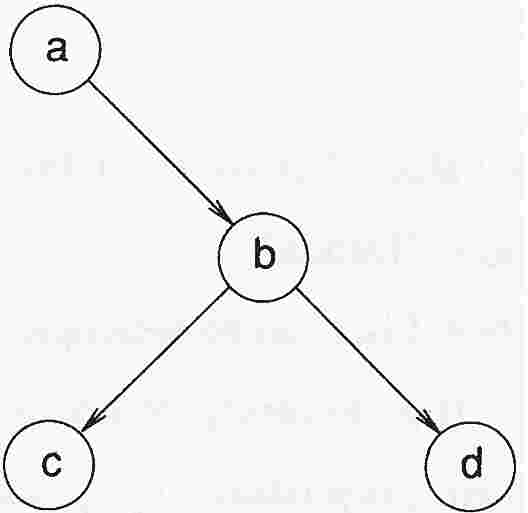
\includegraphics[width=1.8161in,height=1.7134in]{ib-img/ib-img002.jpg} 

Structures also can be used to represent loops, as in

{\ttfamily\mdseries
\ \ \ graph := [{\textquotedbl}a{\textquotedbl}, {\textquotedbl}{\textquotedbl}]\newline
 \ \ graph[2] := graph}

\noindent which can be depicted as

\ \  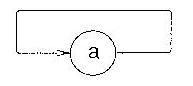
\includegraphics[width=1.4193in,height=0.5992in]{ib-img/ib-img003.jpg} 

Lists are not fixed in size. Elements can be added to them or removed
from them at their ends by queue and stack functions.

The function \texttt{put(a, x)} adds the value of \texttt{x} to the
right end of the increasing its size by one.  Similarly,
\texttt{push(a, x)} adds the value of \texttt{x} to the left end of
\texttt{a}. For example,

{\ttfamily\mdseries
\ \ \ lines := []\newline
 \ \ while put(lines, read(f))}

\noindent constructs a list of the lines from the file f. Conversely,

{\ttfamily\mdseries
\ \ \ lines := []\newline
 \ \ while push(lines, read(f))}

\noindent constructs a list of lines in reverse order.

The functions \texttt{pop(a)} and \texttt{get(a)} are the same. They
both remove an element from the left end of a and return it as the
value of the function call, but they fail if a is empty. Consequently,

{\ttfamily\mdseries
\ \ \ lines := []\newline
 \ \ while push(lines, read(f))\newline
 \ \ while write(pop(lines))}

\noindent writes out the lines of \texttt{f} in reverse order. The
function \texttt{pull(a)} is similar, but it removes an element from
the right end of \texttt{a}.

Other operations on lists include concatenation, which is denoted by

{\ttfamily\mdseries
\ \ \ a1 {\textbar}{\textbar}{\textbar} a2}

\noindent where \texttt{a1} and \texttt{a2} are lists. There is no
automatic conversion of other types to lists.

List sectioning is denoted by

{\ttfamily
\ \ \ a[i:j]}

The result is a \textit{new} list containing values \texttt{i} through
\texttt{j} of \texttt{a}.

There is no inherent limit to the size of a list, either when it is
originally created or as a result of adding elements to it.

{\sffamily\bfseries
2.1.6 Sets}

A set is an unordered collection of values. Unlike csets, which
contain only characters, sets are collections of Icon values that can
be of any type. A set is constructed from a list by
\texttt{set(a)}. For example,

{\ttfamily\mdseries
\ \ \ states := set([{\textquotedbl}Virginia{\textquotedbl}, {\textquotedbl}Rhode Island{\textquotedbl},
{\textquotedbl}Kansas{\textquotedbl}, \ \ \ \ \ \ \ \  \ {\textquotedbl}Illinois{\textquotedbl}])}

\noindent
assigns a set of four elements to \texttt{states}.

The operation

{\ttfamily\mdseries
\ \ \ member(s, x)}

\noindent
succeeds if the value of \texttt{x} is a member of \texttt{s} but
fails otherwise. The operation

{\ttfamily\mdseries
\ \ \ insert(s, x)}

\noindent
adds the value of \texttt{x} to \texttt{s} if it is not already a
member of \texttt{s}, while

{\ttfamily
\ \ \ delete(s, x)}

\noindent
deletes the value of \texttt{x} from \texttt{s}. The operations of
union, intersection, and difference for sets also are provided.

Like other structures, sets can be heterogeneous. A set can even be a
member of itself, as in

{\ttfamily\mdseries
\ \ \ insert(s, s)}

There is no contradiction here, since a set value is a pointer to the
structure for the set.

{\sffamily\bfseries
2.1.7 Tables}

A table is a set of pairs of values. Tables provide an associative
look mechanism as contrasted with positional references to lists. They
can be subscripted with an \textit{entry value }to which a value can
be assigned to make up a pair called a table element.

A table is created by

{\ttfamily\mdseries
\ \ \ table(x)}


Tables are empty initially. The value of x is an assigned default
value that is produced if the table is subscripted with an entry value
to which no value has been assigned (that is, for an element that is
not in the table). For example,

{\ttfamily\mdseries
\ \ \ states := table(0)}

\noindent assigns to states a table with a default value of 0. An
element can be added to states by an assignment such as

{\ttfamily\mdseries
\ \ \ states[{\textquotedbl}Oregon{\textquotedbl}] := 1}

\noindent which adds a table element for
\texttt{{\textquotedbl}Oregon{\textquotedbl}} with the value
\texttt{1} to \texttt{states}. On the other hand,

{\ttfamily\mdseries
\ \ \ write(states [{\textquotedbl}Utah{\textquotedbl}])}

\noindent writes \texttt{0}, the default value, if there is no element
in the table for \texttt{{\textquotedbl}Utah{\textquotedbl}}.

Tables can be heterogeneous and have a mixture of types for entry and
assigned values. Tables grow automatically in size as new elements are
added and there is no inherent limit on the size of a table.

{\sffamily\bfseries
2.1.8 Records}

A record is an aggregate of values that is referenced by named
fields. Each record type has a separate name. A record type and the
names of its fields are given in a declaration. For example,

{\ttfamily\mdseries
\ \ \ record rational(numerator, denominator)}

\noindent
declares a record of type rational with two fields: numerator and denominator.

An instance of a record is created by calling a record-constructor
function corresponding to the form of the declaration for the record
type. Thus,

{\ttfamily\mdseries
\ \ \ r := rational(3,5)}

\noindent
assigns to \texttt{r} a record of type rational with a
numerator field of 3 and a denominator field of 5. Fields are
referenced by name, as in

{\ttfamily\mdseries
\ \ \ write(r.numerator)}

\noindent which writes 3. Fields can also be referred to by position;
\texttt{r[1]} is equivalent to \texttt{r.numerator}.

There is no inherent limit to the number of different record
types. The same field names can be given for different record types,
and such fields need not be in the same position for all such record
types.

{\sffamily\bfseries
2.1.9 Input and Output}

Input and output in Icon are sequential and comparatively simple. The
standard input, standard output, and standard error output files are
the values of \texttt{\&input}, \texttt{\&output}, and
\texttt{\&errout}, respectively. The function

{\ttfamily\mdseries
\ \ \ open(s1,s2)}

\noindent opens the file whose name is \texttt{s1} according to
options given by \texttt{s2} and produces a value of type file.
Typical options are \texttt{{\textquotedbl}r{\textquotedbl}} for
opening for reading and \texttt{{\textquotedbl}w{\textquotedbl}} for
opening for writing. The default is
\texttt{{\textquotedbl}r{\textquotedbl}}. For example,

{\ttfamily\mdseries
\ \ \ log := open({\textquotedbl}grade.log{\textquotedbl}, {\textquotedbl}w{\textquotedbl})}

\noindent assigns a value of type file to log, corresponding to the
data file grade.log, which is opened for writing. The function open
fails if the specified file cannot be opened according to the options
given. The function \texttt{close(f)} closes the file \texttt{f}.

The function \texttt{read(f)} reads a line from the file \texttt{f}
but fails if an end of file is encountered. The default is standard
input if \texttt{f} is omitted.

The result of

{\ttfamily\mdseries
\ \ \ write(x1,x2, ..., xn)}

\noindent depends on the types of x1, x2, ..., xn. Strings and types
convertible to strings are written, but if one of the arguments is a
file, subsequent strings are written to that file. The default file is
standard output. Thus,

{\ttfamily\mdseries
\ \ \ write(s1,s2)}

\noindent
writes the concatenation of \texttt{s1} and \texttt{s2} to standard output, but

{\ttfamily\mdseries
\ \ \ write(log,s)}

\noindent
writes \texttt{s} to the file grade.log. In any event, write returns
the string value of the last argument written.

The function

{\ttfamily\mdseries
\ \ \ stop(x1, x2, ..., xn)}

\noindent
produces the same output as write, but it then terminates program execution.

{\sffamily\bfseries
2.1.10 Procedures}

\textbf{Procedure Declarations.} The executable portions of an Icon
program are contained in procedure declarations.  Program execution
begins with a call of the procedure main.

An example of a procedure declaration is:

{\ttfamily\mdseries
\ \ \ procedure maxstr(slist)\newline
 \ \ \ \ \ local max, value\newline
 \ \ \ \ \ max := 0\newline
 \ \ \ \ \ every value := *!slist do\newline
 \ \ \ \ \ \ \ \ if value{\textgreater} max then max := value\newline
 \ \ \ \ \ return max\newline
 \ \ end}


This procedure computes the longest string in a list of strings. The
formal parameter slist and the identifiers max and value are local to
calls of the procedure \texttt{maxstr()}. Storage for them is
allocated when \texttt{maxstr()} is called and deallocated when
\texttt{maxstr()} returns.

A procedure call has the same form as a function call. For example,

{\ttfamily\mdseries
\ \ \ lines := []\newline
 \ \ while put(lines, read(f))\newline
 \ \ write(maxstr(lines))}

\noindent
writes the length of the longest line in the file \texttt{f}.

A procedure call may fail to produce a result in the same way that a
built-in operation can fail. This is indicated by fail in the
procedure body in place of return. For example, the following
procedure returns the length of the longest string in \texttt{slist}
but fails if that length is less than limit:

{\ttfamily\mdseries
\ \ \ procedure maxstr(slist, limit)\newline
 \ \ \ \ \ local max, value\newline
 \ \ \ \ \ max := 0\newline
 \ \ \ \ \ every value := *!slist do\newline
 \ \ \ \ \ \ \ \ if value{\textgreater} max then max := value\newline
 \ \ \ \ \ if max {\textless} limit then fail else return max\newline
 \ \ end}

Flowing off the end of a procedure body without an explicit return is
equivalent to fail.

A procedure declaration may have static identifiers that are known
only to calls of that procedure but whose values are not destroyed
when a call returns. A procedure declaration also may have an initial
clause whose expression is evaluated only the first time the procedure
is called. The use of a static identifier and an initial clause is
illustrated by the following procedure, which returns the longest of
all the strings in the lists it has processed:

{\ttfamily\mdseries
\ \ \ procedure maxstrall(slist)\newline
 \ \ \ \ \ local value\newline
 \ \ \ \ \ static max\newline
 \ \ \ \ \ initial max := 0\newline
 \ \ \ \ \ every value := *!slist do\newline
 \ \ \ \ \ \ \ \ if value{\textgreater} max then max := value\newline
 \ \ \ \ \ return max\newline
 \ \ end}

\textbf{Procedures and Functions.} Procedures and functions are used
in the same way. Their names have global scope.  Other identifiers can
be declared to have global scope, as in

{\ttfamily\mdseries
\ \ \ global count}

Such global declarations are on a par with procedure declarations and
cannot occur within procedure declarations.

A call such as

{\ttfamily\mdseries
\ \ \ write(maxstr(lines))}

\noindent
applies the \textit{value} of the identifier \texttt{maxstr} to
\texttt{lines} and applies the \textit{value} of the identifier
\texttt{write} to the result. There is nothing fixed about the values
of such identifiers. In this case, the initial value of
\texttt{maxstr} is a procedure, as a consequence of the procedure
declaration for it. Similarly, the initial value of \texttt{write} is
a function. These values can be assigned to other variables, as in

{\ttfamily\mdseries
\ \ \ print := write\newline
 \ \ \ \ \ \ \ \ \ \ ...\newline
 \ \ \textrm{print(maxstr(lines))}}

\noindent in which the function that is the initial value of
\texttt{write} is assigned to \texttt{print}.

Similarly, nothing prevents an assignment to an identifier whose
initial value is a procedure. Consequently,

{\ttfamily\mdseries
\ \ \ write := 3}

\noindent
assigns an integer to \texttt{write}, replacing its initial function value.

Although it is typical to call a procedure by using an identifier that
has the procedure value, the procedure used in a call can be
computed. The general form of a call is

{\ttfamily\mdseries
\textit{\ \ \ expr}\textit{\TextSubscript{0}}\textit{(expr}\textit{\TextSubscript{1}}\textit{,
expr}\textit{\TextSubscript{2}}\textit{, }..., \textit{expr}\textit{\TextSubscript{n}}\textit{)}}

\noindent where the value of
\textit{expr\TextSubscript{0}} is applied to the
arguments resulting from the evaluation of
\textit{expr\TextSubscript{1}}
\textit{expr\TextSubscript{2}}, ...,
\textit{expr\TextSubscript{n}}. For example,

{\ttfamily\mdseries
\ \ \ (proclist[i])\textit{(expr\TextSubscript{1}}, ,
\textit{expr\TextSubscript{2}},
..., \textit{expr\TextSubscript{n})}}

\noindent
applies the procedure that is the \texttt{i}th element of \texttt{proclist}.

Procedures may be called recursively. The recursive nature of a call
depends on the fact that procedure names are global. The
{\textquotedbl}Fibonacci strings{\textquotedbl} provide an example:

{\ttfamily\mdseries
\ \ \ procedure fibstr(i)\newline
 \ \ \ \ \ if i = 1 then return {\textquotedbl}a{\textquotedbl}\newline
 \ \ \ \ \ else if i = 2 then return {\textquotedbl}b{\textquotedbl}\newline
 \ \ \ \ \ else return fibstr(i - 1) {\textbar}{\textbar} fibstr(i - 2)\newline
 \ \ end}

An identifier that is not declared in a procedure and is not global
defaults to local. Thus, local declarations can be omitted, as in

{\ttfamily\mdseries
\ \ \ procedure maxstr(slist)\newline
 \ \ \ \ \ max := 0\newline
 \ \ \ \ \ every value := * !slist do\newline
 \ \ \ \ \ \ \ \ if value {\textgreater} max then max := value\newline
 \ \ \ \ \ return max\newline
 \ \ end}


\textbf{Procedures as Generators}. In addition to returning and
failing, a procedure can also suspend. In this case, the values of its
arguments and local identifiers are not destroyed, and the call can
be resumed to produce another result in the same way a built-in
generator can be resumed. An example of such a generator is

{\ttfamily\mdseries
\ \ \ procedure intseq(i)\newline
 \ \ \ \ \ repeat \{\newline
 \ \ \ \ \ \ \ \ suspend i\newline
 \ \ \ \ \ \ \ \ i +:= 1\newline
 \ \ \ \ \ \ \ \ \}\newline
 \ \ end}

A call \texttt{intseq(10)}, for example, is capable of generating the
infinite sequence of integers 10, 11, 12, ... .  For example,

{\ttfamily\mdseries
\ \ \ every f(intseq(10) {\textbackslash} 5)}

\noindent
calls f(10), f(11), f(12), f(13), and f(14).

If the argument of suspend is a generator, the generator is resumed
when the call is resumed and the call suspends again with the result
it produces. A generator of the Fibonacci strings provides an example:

\ \ \ procedure fibstrseq()\newline
 \ \ \ \ \ local s1, s2, s3\newline
 \ \ \ \ \ s1 := {\textquotedbl}a{\textquotedbl}\newline
 \ \ \ \ \ s2 := {\textquotedbl}b{\textquotedbl}\newline
 \ \ \ \ \ suspend (s1 {\textbar} s2)\newline
 \ \ \ \ \ repeat \{\newline
 \ \ \ \ \ \ \ \ suspend s3 := s1 {\textbar}{\textbar} s2\newline
 \ \ \ \ \ \ \ \ s1 := s2\newline
 \ \ \ \ \ \ \ \ s2 := s3\newline
 \ \ \ \ \ \ \ \ \}\newline
 \ \ end

When this procedure is called, the first suspend expression produces
the value of\ \ s1, {\textquotedbl}a{\textquotedbl}. If the call of
\texttt{fibstrseq()} is resumed, the argument of \texttt{suspend} is
resumed and produces the value of \texttt{s2},
\texttt{{\textquotedbl}b{\textquotedbl}}. If the call is resumed
again, there is no further result for the first \texttt{suspend}, and
evaluation continues to the \texttt{repeat} loop.

Repeated alternation often is useful in supplying an endless number of
alternatives. For example, the procedure \texttt{intseq(i)} can be
rewritten as

{\ttfamily\mdseries
\ \ \ procedure intseq(i)\newline
 \ \ \ \ \ suspend i {\textbar} (i +:= {\textbar}1)\newline
 \ \ end}

Note that \texttt{{\textbar}1} is used to provide an endless sequence
of increments.


\textbf{Argument Transmission}. Omitted arguments in a procedure or
function call (including trailing ones) default to the null
value. Extra arguments are evaluated, but their values are discarded.

Some functions, such as \texttt{write()}, may be called with an
arbitrary number of arguments. All arguments to procedures and
functions are passed by value. If the evaluation of an argument
expression fails, the procedure or function is not called. This
applies to extra arguments. Arguments are not dereferenced until all
of them have been evaluated. Dereferencing cannot fail. Since no
argument is dereferenced until all argument expressions are evaluated,
expressions with side effects can produce unexpected results. Thus, in

{\ttfamily\mdseries
\ \ \ write(s, s := {\textquotedbl}hello{\textquotedbl})}

\noindent the value written is \texttt{hellohello}, regardless of the
value of \texttt{s} before the evaluation of the second argument of
\texttt{write()}.


\textbf{Dereferencing in Return Expressions}. The result returned from
a procedure call is dereferenced unless it is a global identifier, a
static identifier, a subscripted structure, or a subscripted
string-valued global identifier.

In these exceptional cases, the variable is returned and assignment
can be made to the procedure call. An example is

{\ttfamily\mdseries
\ \ \ procedure maxel(a, i, j)\newline
 \ \ \ \ \ if i {\textgreater} j then return a[i]\newline
 \ \ \ \ \ else return a[j]\newline
 \ \ end}

Here a list element, depending on the values of \texttt{i} and
\texttt{j}, is returned. An assignment can be made to it, as in

{\ttfamily\mdseries
\ \ \ maxel(lines, i, j) := {\textquotedbl}end{\textquotedbl}}

\noindent which assigns \texttt{{\textquotedbl}end{\textquotedbl}} to
\texttt{lines[i]} or \texttt{lines[j]}, depending on the values of
\texttt{i} and \texttt{j}.


\textbf{Mutual Evaluation}. In a call expression, the value of
\textit{expr}\textit{\TextSubscript{0}} can be an integer
\texttt{i} as well as a procedure. In this case, called
\textit{mutual evaluation}, the result of the \texttt{i}th
argument is produced. For example,

{\ttfamily\mdseries
\ \ \ i := 1(find(s1, line1), find(s2, line2))}

\noindent assigns to \texttt{i} the position of \texttt{s1} in
\texttt{line1}, provided \texttt{s1} occurs in \texttt{line1} and that
\texttt{s2} occurs in line2. If either call of find fails, the
expression fails and no assignment is made.

The selection integer in mutual evaluation can be negative, in which
case it is interpreted relative to the end of the argument
list. Consequently,

{\ttfamily\mdseries
\textit{\ \ \ (-1)(expr\TextSubscript{1}},\textit{expr\TextSubscript{2}}\textit{, }...,
\textit{expr\TextSubscript{n}}\textit{)}}

\noindent
produces the result of \textit{expr\TextSubscript{n}} and is equivalent to


\textit{\ \ \ expr1 }\& \textit{expr2 }\& ... \& \textit{exprn}

The selection integer can be omitted, in which case it defaults to -1.


{\sffamily\bfseries
2.1.11 Co-Expressions}

The evaluation of an expression in Icon is limited to the site in the
program where it appears. Its results can be produced only at that
site as a result of iteration or goal-directed evaluation. For
example, the results generated by \texttt{intseq(i)} described in
Section 2.1.10 can only be produced where it is called, as in

{\ttfamily\mdseries
\ \ \ every f(intseq(10) {\textbackslash} 5)}

It is often useful, however, to be able to produce the results of a
generator at various places in the program as the need for them
arises. Co-expressions provide this facility by giving a context for
the evaluation of an expression that is maintained in a data
structure. Co-expressions can be \textit{activated }to produce the
results of a generator on demand, at any time and place in the
program.

A co-expression is constructed by

\ \ \ create \textit{expr}

The expression \textit{expr} is not evaluated at this time. Instead,
an object is produced through which \textit{expr} can be resumed at a
later time. For example,

{\ttfamily\mdseries
\ \ \ label := create ({\textquotedbl}L{\textquotedbl} {\textbar}{\textbar} (1 to 100) {\textbar}{\textbar}
{\textquotedbl}:{\textquotedbl})}

\noindent assigns to label a co-expression for the expression

{\ttfamily\mdseries
\ \ \ {\textquotedbl}L{\textquotedbl} {\textbar}{\textbar} (1 to 100) {\textbar}{\textbar}
{\textquotedbl}:{\textquotedbl}}

The operation \texttt{@label} activates this co-expression, which
corresponds to resuming its expression. For example,

{\ttfamily\mdseries
\ \ \ write(@label)\newline
 \ \ write({\textquotedbl} \ \ \ tstl \ \ \ \ count{\textquotedbl})\newline
 \ \ write(@label)}

\noindent
writes

{\ttfamily\mdseries
\ \ \ L1:\newline
 \ \ \ \ \ \ \ tstl \ \ \ \ count\newline
 \ \ L2:}

If the resumption of the expression in a co-expression does not
produce a result, the co-expression activation fails.  For example,
after \texttt{@label} has been evaluated 100 times, subsequent
evaluations of \texttt{@label} fail. The number of results that a
co-expression \texttt{e} has produced is given by \texttt{*e}.

The general form of the activation expression is

\textit{\ \ \ expr1 }@ \textit{expr2}

\noindent which activates \textit{expr2} and transmits the result of
\textit{expr1} to it. This form of activation can be used to return a
result to the co-expression that activated the current one.

A co-expression is a value like any other value in Icon and can be
passed as an argument to a procedure, returned from a procedure. and
so forth. A co-expression can survive the call of the procedure in
which it is created.

If the argument of a create expression contains identifiers that are
local to the procedure in which the create occurs, copies of these
local identifiers are included in the co-expression with the values
they have at the time the create expression is evaluated. These copied
identifiers subsequently are independent of the local identifiers in
the procedure. Consider, for example,

{\ttfamily\mdseries
\ \ \ procedure labgen(tag)\newline
 \ \ \ \ \ local i, j\newline
\ \  ...\newline
\ \  i := 10\newline
\ \  j := 20\newline
\ \  e := create (tag {\textbar}{\textbar} (i to j) {\textbar}{\textbar} {\textquotedbl}:{\textquotedbl})\newline
\ \  ...\newline
\ \  i := j\newline
\ \  if i {\textgreater} 15 then return e\newline
\ \  ...\newline
 \ \ end}

The expression

{\ttfamily\mdseries
\ \ \ labels := labgen({\textquotedbl}X{\textquotedbl})}

\noindent assigns to labels a co-expression that is equivalent to evaluating

{\ttfamily\mdseries
\ \ \ create ({\textquotedbl}X{\textquotedbl} {\textbar}{\textbar} (10 to 20) {\textbar}{\textbar}
{\textquotedbl}:{\textquotedbl})}

The fact that \texttt{i} is changed after the co-expression was
assigned to \texttt{e}, but before \texttt{e} returns, does not affect
the co-expression, since it contains copies of \texttt{i} and
\texttt{j} at the time it was created.  Subsequent changes to the
values of \texttt{i} or \texttt{j} do not affect the co-expression.

A copy of a co-expression \texttt{e} is produced by the
\textit{refresh }operation, \texttt{\^{}e}. When a refreshed copy of a
co-expression is made, its expression is reset to its initial state,
and the values of any local identifiers in it are reset to the values
they had when the co-expression was created. For example,

{\ttfamily\mdseries
\ \ \ newlabels := \^{}labels}

\noindent assigns to \texttt{newlabels} a co-expression that is
capable of producing the same results as labels, regardless of whether
or not labels has been activated.

The value of the keyword \texttt{\&main} is the co-expression for the
call of \texttt{main()} that initiates program execution.


{\sffamily\bfseries
2.1.12 Diagnostic Facilities}

\textbf{String Images}. The function \texttt{type(x)} only produces
the string name of the type of \texttt{x}, but the function
\texttt{image(x)} produces a string that shows the value of
\texttt{x}. For strings and csets, the value is shown with surrounding
quotation marks in the fashion of program literals. For example,

{\ttfamily\mdseries
\ \ \ write(image({\textquotedbl}Hi there!{\textquotedbl}))}

\noindent writes \texttt{{\textquotedbl}Hi there!{\textquotedbl}}, while

{\ttfamily\mdseries
\ \ \ write(image('aeiou'))}

\noindent writes \texttt{{}'aeiou'}.

For structures, the type name and size are given. For example,

{\ttfamily\mdseries
\ \ \ write(image([]))}

\noindent writes \texttt{list(0)}.

Various forms are used for other types of data, using type names where
necessary so that different types of values are distinguishable.


\textbf{Tracing}. If the value of the keyword \texttt{\&trace} is
nonzero, a trace message is produced whenever a procedure is called,
returns, fails, suspends, or is resumed. Trace messages are written to
standard error output. The value of \texttt{\&trace} is decremented
for every trace message. Tracing stops if the value of
\texttt{\&trace} becomes zero, which is its initial value. Suppose
that the following program is contained in the file fibstr.icn:

{\ttfamily\mdseries
\ \ \ procedure main()\newline
 \ \ \ \ \ \&trace := -1\newline
 \ \ \ \ \ fibstr(3)\newline
 \ \ end\newline
\newline
 \ \ procedure fibstr(i)\newline
 \ \ \ \ \ if i = 1 then return {\textquotedbl}a{\textquotedbl}\newline
 \ \ \ \ \ else if i = 2 then return {\textquotedbl}b{\textquotedbl}\newline
 \ \ \ \ \ else return fibstr(i -1) {\textbar}{\textbar} fibstr(i -2)\newline
 \ \ end}

The trace output of this program is

{\ttfamily\mdseries
\textrm{\ \ \ fibstr.icn: 3\ \ {\textbar} fibstr(3)}\newline
 \ \ fibstr.icn: 9\ \ {\textbar} {\textbar} fibstr(2)\newline
 \ \ fibstr.icn: 8\ \ {\textbar} {\textbar} fibstr returned {\textquotedbl}b{\textquotedbl}\newline
 \ \ fibstr .icn: 9\ \ {\textbar} {\textbar} fibstr(1)\newline
 \ \ fibstr.icn: 7\ \ {\textbar} {\textbar} fibstr returned {\textquotedbl}b{\textquotedbl}\newline
 \ \ fibstr.icn: 9\ \ {\textbar} fibstr returned {\textquotedbl}ba{\textquotedbl}\newline
 \ \ fibstr.icn: 4\ \ main failed}

In addition to the indentation corresponding to the level of procedure
call, the value of the keyword \texttt{\&level} also is the current
level of call.

\textbf{Displaying Identifier Values}. The function
\texttt{display(i,f)} writes a list of all identifiers and their
values for \texttt{i} levels of procedure calls, starting at the
current level. If \texttt{i} is omitted, the default is
\texttt{\&level}, while if \texttt{f} is omitted, the list is written
to standard error output. The format of the listing produced by
display is illustrated by the following program:

{\ttfamily
\ \ \ procedure main()\newline
 \ \ \ \ \ log := open({\textquotedbl}grade.log{\textquotedbl}, {\textquotedbl}w{\textquotedbl})\newline
 \ \ \ \ \ while write(log, check(readO))\newline
 \ \ end}


\bigskip

{\ttfamily
\ \ \ procedure check(value)\newline
 \ \ \ \ \ static count\newline
 \ \ \ \ \ initial count := 0\newline
 \ \ \ \ \ if numeric(value) then \{\newline
 \ \ \ \ \ \ \ \ count +:= 1\newline
 \ \ \ \ \ \ \ \ return value\newline
 \ \ \ \ \ \ \ \ \}\newline
 \ \ \ \ \ else \{\newline
 \ \ \ \ \ \ \ \ display()\newline
 \ \ \ \ \ \ \ \ stop({\textquotedbl}nonnumeric value{\textquotedbl})\newline
 \ \ \ \ \ \ \ \ \}\newline
 \ \ end}


Suppose that the tenth line of input is the nonnumeric string
\texttt{{\textquotedbl}3.a{\textquotedbl}}. Then the output of
\texttt{display()} is

{\ttfamily\mdseries
\ \ \ check local identifiers:\newline
 \ \ \ \ \ value = {\textquotedbl}3.a{\textquotedbl}\newline
 \ \ \ \ \ count = 9\newline
 \ \ main local identifiers:\newline
 \ \ \ \ \ log = file(grade.log)\newline
 \ \ global identifiers:\newline
 \ \ \ \ \ main = procedure main\newline
 \ \ \ \ \ check = procedure check\newline
 \ \ \ \ \ open = function open\newline
 \ \ \ \ \ write = function write\newline
 \ \ \ \ \ read = function read\newline
 \ \ \ \ \ numeric = function numeric\newline
 \ \ \ \ \ display = function display\newline
 \ \ \ \ \ stop = function stop}


\textbf{Error Messages}. If an error is encountered during program
execution, a message is written to standard error output and execution
is terminated. For example, if the tenth line of a program contained
in the file check.icn is

{\ttfamily\mdseries
\ \ \ i +:= {\textquotedbl}x{\textquotedbl}}

\noindent
evaluation of this expression produces the error message

{\ttfamily\mdseries
\ \ \ Run-time error 102 at line 10 in check.icn\newline
 \ \ numeric expected\newline
 \ \ offending value: {\textquotedbl}x{\textquotedbl}}


\section[2.2 Language Features and the Implementation]{2.2 Language Features and the Implementation}

Even a cursory consideration of Icon reveals that some of its features
present implementation problems and require approaches that are
different from ones used in more conventional languages. In the case
of a language of the size and complexity of Icon, it is important to
place different aspects of the implementation in perspective and to
identify specific problems.


\textbf{Values and Variables.} The absence of type declarations in
Icon has far-reaching implications. Since any variable may have a
value of any type and the type may change from time to time during
program execution, there must be a way of representing values
uniformly. This is a significant challenge in a language with a wide
variety of types ranging from integers to
co-expressions. Heterogeneous structures follow as a natural
consequence of the lack of type declarations.

In one sense, the absence of type declarations simplifies the
implementation: there is not much that can be done about types during
program translation (compilation), and some of the work that is
normally performed by conventional compilers can be avoided. The
problems do not go away, however -- they just move to another part of
the implementation, since run-time type checking is
required. Automatic type conversion according to context goes
hand-in-hand with type checking.


\textbf{Storage Management.} Since strings and structures are created
during program execution, rather than being declared, the space for
them must be allocated as needed at run time. This implies, in turn,
some mechanism for reclaiming space that has been allocated but which
is no longer needed--{\textquotedbl}garbage collection.{\textquotedbl}
These issues are complicated by the diversity of types and sizes of
objects, the lack of any inherent size limitations, and the
possibility of pointer loops in circular structures.


\textbf{Strings.} Independent of storage-management considerations,
strings require special attention in the implementation. The emphasis
of Icon is on string processing, and it is necessary to be able to
process large amounts of string data sufficiently. Strings may be very
long and many operations produce substrings of other strings. The
repertoire of string analysis and string synthesis functions is
large. All this adds up to the need for a well-designed and coherent
mechanism for handling strings.


\textbf{Structures.} Icon's unusual structures, with sophisticated
access mechanisms, also pose problems. In particular, structures that
can change in size and can grow without limit require different
implementation approaches than static structures of fixed size and
organization.


The flexibility of positional, stack, and queue access mechanisms for
lists requires compromises to balance efficient access for different
uses. Sets of values with arbitrary types, combined with a range of
set operations, pose non-trivial implementation problems. Tables are
similar to sets, but require additional attention because of the
implicit way that elements are added.


\textbf{Procedures and Functions.} Since procedures and functions are
values, they must be represented as data objects.  More significantly,
the meaning of a function call cannot, in general, be determined when
a program is translated. The expression write(s) may write a string or
it may do something else, depending on whether or not write still has
its initial value. Such meanings must, instead, be determined at run
time.


\textbf{Polymorphic Operations.} Although the meanings of operations
cannot be changed during program execution in the way that the
meanings of calls can, several operations perform different
computations depending on the types of their operands. Thus, x[i] may
subscript a string, a list, or a table.

The meanings of some operations also depend on whether they occur in
an assignment or a dereferencing context. For example, if s has a
string value, assignment to s [i] is an abbreviation for a
concatenation followed by an assignment to s, while if s[i] occurs in
a context where its value is needed, it is simply a substring
operation. Moreover, the context cannot, in general, be determined at
translation time.

The way subscripting operations are specified in Icon offers
considerable convenience to the programmer at the expense of
considerable problems for the implementer.


\textbf{Expression Evaluation.} Generators and goal-directed
evaluation present obvious implementation problems. There is a large
body of knowledge about the implementation of expression evaluation
for conventional languages in which expressions always produce a
single result, but there is comparatively little knowledge about
implementing expressions that produce results in sequence.

While there are languages in which expressions can produce more than
one result, this capability is limited to specific contexts, such as
pattern matching, or to specific control structures or data objects.

In Icon, generators and goal-directed evaluation are general and
pervasive and apply to all evaluation contexts and to all types of
data. Consequently, their implementation requires a fresh
approach. The mechanism also has to handle the use of failure to drive
control structures and must support novel control structures, such as
alternation and limitation. Efficiency is a serious concern, since
whatever mechanism is used to implement generators is also used in
conventional computational situations in which only one result is
needed.


\textbf{String Scanning.} String scanning is comparatively simple. The
subject and position --- {\textquotedbl}state variables{\textquotedbl}
--- have to be saved at the beginning of string scanning and restored
when it is completed.  Actual string analysis and matching follow
trivially from generators and goal-directed evaluation.


\textbf{Co-Expressions.} Co-expressions, which are only relevant
because of the expression-evaluation mechanism of Icon, introduce a
whole new set of complexities. Without co-expressions, the results
that a generator can produce are limited to its site in the
program. Control backtracking is limited syntactically, and its scope
can be determined during program translation. With co-expressions, a
generator in a state of suspension can be activated at any place and
time during program execution.


\textsc{Retrospective}: Icon has a number of unusual features that are
designed to facilitate programming, and it has an extensive repertoire
of string and structure operations. One of Icon's notable
characteristics is the freedom from translation-time constraints and
the ability to specify and change the meanings of operations at run
time. This run-time flexibility is valuable to the programmer, but it
places substantial burdens on the implementation---and also makes it
interesting.

At the top level, there is the question of how actually to carry out
some of the more sophisticated operations. Then there are questions of
efficiency, both in execution speed and storage utilization. There are
endless possibilities for alternative approaches and refinements.

It is worth noting that many aspects of the implementation are
relatively independent of each other and can be approached
separately. Operations on strings and structures are largely disjoint
and can, except for general considerations of the representation of
values and storage management, be treated as independent problems.

The independence of expression evaluation from other implementation
considerations is even clearer. Without generators and goal-directed
evaluation, Icon would be a fairly conventional high-level string and
structure processing language, albeit one with interesting
implementation problems. On the other hand, generators and
goal-directed evaluation are not dependent in any significant way on
string and structure data types. Generators, goal-directed evaluation,
and related control structures could just as well be incorporated in a
programming language emphasizing numerical computation. The
implementation problems related to expression evaluation in the two
contexts are largely the same.

While untyped variables and automatic storage management have
pervasive effects on the overall implementation of Icon, there are
several aspects of Icon that are separable from the rest of the
language and its implementation. Any specific data structure, string
scanning, or co-expressions could be eliminated from the language
without significantly affecting the rest of the
implementation. Similarly, new data structures and new access
mechanisms could be added without requiring significant modifications
to the balance of the implementation.

{\sffamily\bfseries
EXERCISES}

\liststyleLi
\begin{enumerate}
\item \begin{enumerate}
\item 
\ What is the outcome of the following expression if the file f contains a line consisting of
{\textquotedbl}end{\textquotedbl}, or if it does not?\newline
 \ \ \ \ while line := read(f) do\newline
 \ \ \ \ \ \ \ \ \ if line == {\textquotedbl}end{\textquotedbl} then break\newline
 \ \ \ \ \ \ \ \ \ else write(line)
\item 
\ What does\newline
 \ \ \ \ \ write({\textquotedbl}hello{\textquotedbl} {\textbar} {\textquotedbl}howdy{\textquotedbl})\newline
write?
\item 
\ What is the result of evaluating the following expression:\newline
\texttt{ \ \ \ \ \ 1(1 to 3) {\textgreater} 10}
\item 
\ Explain the rationale for dereferencing of variables when a procedure call returns.
\item 
\ Give an example of a situation in which it cannot be determined until run time whether a string subscripting
expression is used in an assignment or a dereferencing context.
\end{enumerate}
\end{enumerate}

\chapter{Organization of the Implementation}

\textsc{Perspective}: Many factors influence the implementation of a
programming language. The properties of the language itself, of
course, are of paramount importance. Beyond this, goals, resources,
and many other factors may affect the nature of an implementation in
significant and subtle ways.

In the case of the implementation of Icon described here, several
unusual factors deserve mention. To begin with, Icon's origins were in
a research project, and its implementation was designed not only to
make the language available for use but also to support further
language development. The language itself was less well defined and
more subject to modification than is usually the case with an
implementation. Therefore, flexibility and ease of modification were
important implementation goals.

Although the implementation was not a commercial enterprise, neither
was it a toy or a system intended only for a few ``friendly users.''
It was designed to be complete, robust, easy to maintain, and
sufficiently efficient to be useful for real applications in its
problem domain.

Experience with earlier implementations of SNOBOL4, SL5, and the
Ratfor implementation of Icon also influenced the implementation that
is described here. They provided a repertoire of proven techniques and
a philosophy of approach to the implementation of a programming
language that has novel features.

The computing environment also played a major role. The implementation
started on a PDP-11/70 running under UNIX. The UNIX environment
(Ritchie and Thompson 1978), with its extensive range of tools for
program development, influenced several aspects of the implementation
in a direct way. C (Kernighan and Ritchie 1978) is the natural
language for writing such an implementation under UNIX, and its use
for the majority of Icon had pervasive effects, which are described
throughout this book. Tools, such as the Yacc parser-generator
(Johnson 1975), influenced the approach to the translation portion of
the implementation.

Since the initial work was done on a PDP-11/70, with a user address
space of only l28K bytes (combined instruction and data spaces), the
size of the implementation was a significant concern. In particular,
while the Ratfor implementation of Icon fit comfortably on computers
with large address spaces, such as the DEC-10, CDC Cyber, and IBM 370,
this implementation was much too large to fit on a PDP-11/70.

\section[3.1 The Icon Virtual Machine]{3.1 The Icon Virtual Machine}

The implementation of Icon is organized around a virtual machine
(Newey, Poole, and Waite 1972; Griswold 1977). Virtual machines,
sometimes called abstract machines, serve as software design tools for
implementations in which the operations of a language do not fit a
particular computer architecture or where portability is a
consideration and the attributes of several real computer
architectures can be abstracted in a single common model. The
expectation for most virtual machine models is that a translation will
be performed to map the virtual machine operations onto a specific
real machine. A virtual machine also provides a basis for developing
an operational definition of a programming language in which details
can be worked out in concrete terms.

During the design and development phases of an implementation, a
virtual machine serves as an idealized model that is free of the
details and idiosyncrasies of any real machine. The virtual machine
can be designed in such a way that treatment of specific,
machine-dependent details can be deferred until it is necessary to
translate the implementation of the virtual machine to a real one.

Icon's virtual machine only goes so far. Unlike the SNOBOL4 virtual
machine (Griswold 1972), it is incomplete and characterizes only the
expression-evaluation mechanism of Icon and computations on Icon
data. It does not, \textit{per se, }include a model for the
organization of memory. There are many aspects of the Icon run-time
system, such as type checking, storage allocation and garbage
collection, that are not represented in the virtual machine. Instead
Icon's virtual machine serves more as a guide and a tool for
organizing the implementation than it does as a rigid structure that
dominates the implementation.


\section[3.2 Components of the Implementation]{3.2 \textbf{Components of the Implementation}}

There are three major components of the virtual machine implementation
of Icon: a translator, a linker, and a run-time system. The translator
and linker are combined to form a single executable program, but they
remain logically independent.

The translator plays the role of a compiler for the Icon virtual
machine. It analyzes source programs and converts them to virtual
machine instructions. The output of the translator is called
\textit{ucode}. Ucode is represented as ASCII which is helpful in
debugging the implementation.

The linker combines one or more ucode files into a single program for
the virtual machine. This allows programs to be written and translated
in a number of modules, and it is particularly useful for giving users
access to pretranslated libraries of Icon procedures. The output of
the linker, called \textit{icode, }is in binary format for compactness
and ease of processing by the virtual machine. Ucode and icode
instructions are essentially the same, differing mainly in their
format.

Translating and linking are done in two phases:

\begin{picture}(400, 60)(10,0)
\put(-5,30){Icon program}
\put(100,19){\framebox(60,30){translator}}
\put(210,30){ucode}
\put(280,19){\framebox(60,30){linker}}
\put(380,30){icode}
\multiput(75,33)(90,0){4}{\vector(1,0){20}}
\end{picture}

These phases can be performed separately. If only the first phase is
performed, the result is ucode, which can be saved and linked at
another time.

The run-time system consists of an interpreter for icode and a library
of support routines to carry out the various operations that may occur
when an Icon program is executed. The interpreter serves,
conceptually, as a software realization of the Icon virtual
machine. It decodes icode instructions and their operands and carries
out the corresponding operations.

It is worth noting that the organization of the Icon system does not
depend in any essential way on the use of an interpreter. In fact, in
the early versions of this implementation, the linker produced
assembly-language code for the target machine. That code then was
assembled and loaded with the run-time library. On the surface, the
generation of machine code for a specific target machine rather than
for a virtual machine corresponds to the conventional compilation
approach. However, this is somewhat of an illusion, since the machine
code consists largely of calls to run-time library routines
corresponding to virtual machine instructions. Execution of machine
code in such an implementation therefore differs only slightly from
interpretation, in which instruction decoding is done in software
rather than in hardware. The difference in speed in the case of Icon
is relatively minor.

An interpreter offers a number of advantages over the generation of
machine code that offset the small loss of efficiency. The main
advantage is that the interpreter gets into execution very quickly,
since it does not require a loading phase to resolve assembly-language
references to library routines. Icode files also are much smaller than
the executable binary files produced by a loader, since the run-time
library does not need to be included in them. Instead, only one
sharable copy of the run-time system needs to be resident in memory
when Icon is executing.


\section[3.3 The Translator]{3.3 The Translator}

The translator that produces ucode is relatively conventional. It is
written entirely in C and is independent of the architecture of the
target machine on which Icon runs. Ucode is portable from one target
machine to another.

The translator consists of a lexical analyzer, a parser, a code
generator, and a few support routines. The lexical analyzer converts a
source-language program into a stream of tokens that are provided to
the parser as they are needed.  The parser generates abstract syntax
trees on a per-procedure basis. These abstract syntax trees are in
turn processed by the code generator to produce ucode. The parser is
generated automatically by Yacc from a grammatical specification.
Since the translator is relatively conventional and the techniques
that it uses are described in detail elsewhere (Aho, Lam, Sethi, and
Ullman 2006), it is not discussed here.

There is one aspect of lexical analysis that deserves mention. The
body of an Icon procedure consists of a series of expressions that are
separated by semicolons. However, these semicolons usually do not need
to be provided explicitly, as illustrated by examples in Chapter
2. Instead, the lexical analyzer performs semicolon insertion. If a
line of a program ends with a token that is legal for ending an
expression, and if the next line begins with a token that is legal for
beginning an expression, the lexical analyzer generates a semicolon
token between the lines. For example, the two lines

\iconcode{
\>i := j\textit{ }+ 3\\
\>write(i)
}

\noindent are equivalent to

\iconcode{
\>i := j + 3;\\
\>write(i)
}

\noindent since an integer literal is legal at the end of an
expression and an identifier is legal at the beginning of an
expression.

If an expression spans two lines, the place to divide it is at a token
that is not legal at the end of a line. For example,

\iconcode{
\>s1 := s2 ||\\
\>\>s3
}

\noindent is equivalent to

\iconline{
\>s1 := s2 || s3
}

\noindent No semicolon is inserted, since
\texttt{{\textbar}{\textbar}} is not legal at the end of an
expression.

\section[3.4 The Linker]{3.4 The Linker}

The linker reads ucode files and writes icode files. An icode file
consists of an executable header that loads the run-time system,
descriptive information about the file, operation codes and operands,
and data specific to the program. The linker, like the translator, is
written entirely in C. While conversion of ucode to icode is largely a
matter of reformatting, the linker performs two other functions.

\subsection[3.4.1 Scope Resolution]{3.4.1 Scope Resolution}

The scope of an undeclared identifier in a procedure depends on global
declarations (explicit or implicit) in the program in which the
procedure occurs. Since the translator in general operates on only one
module of a program, it cannot resolve the scope of undeclared
identifiers, because not all global scope information is contained in
any one module. The linker, on the other hand, processes all the
modules of a program, and hence it has the task of resolving the scope
of undeclared identifiers.

An identifier may be global for several reasons:

\liststyleLii
\begin{itemize}
\item 
\ As the result of an explicit global declaration.
\item 
\ As the name in a record declaration.
\item 
\ As the name in a procedure declaration.
\item 
\ As the name of a built-in function.
\end{itemize}

If an identifier with no local declaration falls into one of these
categories, it is global. Otherwise it is local.

\subsection[3.4.2 Construction of Run-Time Structures]{3.4.2 Construction of Run-Time Structures}

A number of aspects of a source-language Icon program are represented
at run time by various data structures. These structures are described
in detail in subsequent chapters. They include procedure blocks,
strings, and blocks for cset and real literals that appear in the
program.


This data is represented in ucode in a machine-independent
fashion. The linker converts this information into binary images that
are dependent on the architecture of the target computer.

\section[3.5 The Run{}-Time System]{3.5 The Run-Time System}

Most of the interesting aspects of the implementation of Icon reside
in its run-time system. This run-time system is written mostly in C,
although there are a few lines of assembly-language code for checking
for arithmetic overflow and for co-expressions. The C portion is
mostly machine-independent and portable, although some
machine-specific code is needed for some idiosyncratic computer
architectures and to interface some operating-system environments.

There are two main reasons for concentrating the implementation in the
run-time system:

\liststyleLiii
\begin{itemize}

\item Some features of Icon do not lend themselves to translation
directly into executable code for the target machine, since there is
no direct image for them in the target-machine architecture. The
target machine code necessary to carry out these operations therefore
is too large to place in line; instead, it is placed in library
routines that are called from in-line code. Such features range from
operations on structures to string scanning.

\item Operations that cannot be determined at translation time must be
done at run time. Such operations range from type checking to storage
allocation and garbage collection.

\end{itemize}

The run-time system is logically divided into four main parts:
initialization and termination routines, the interpreter, library
routines called by the interpreter, and support routines called by
library routines.


\textbf{Initialization and Termination Routines.}\ \ The
initialization routine sets up regions in which objects created at run
time are allocated. It also initializes some structures that are used
during program execution. Once these tasks are completed, control is
transferred to the Icon interpreter.

When a program terminates, either normally or because of an error,
termination routines flush output buffers and return control to the
operating system.

\textbf{The Interpreter.} The interpreter analyzes icode instructions
and their operands and performs corresponding operations. The
interpreter is relatively simple, since most complex operations are
performed by library routines. The interpreter itself is described in
Chapter 8.

\textbf{Library Routines. }Library routines are divided into three
categories, depending on the way they are called by the interpreter:
routines for Icon operators, routines for Icon built-in functions, and
routines for complicated virtual machine instructions.

The meanings of operators are known to the translator and linker, and
hence they can be called directly. On the other hand, the meanings of
functions cannot be determined until they are executed, and hence they
are called indirectly.

\textbf{Support Routines. }Support routines include storage allocation
and garbage collection, as well as type checking and conversion. Such
routines typically are called by library routines, although some are
called by other support routines.

\textsc{Retrospective}: Superficially, the implementation of Icon
appears to be conventional. An Icon program is translated and linked
to produce an executable binary file. The translator and linker
\textit{are }conventional, except that they generate code and data
structures for a virtual machine instead of for a specific computer.

The run-time system dominates the implementation and plays a much
larger role than is played by run-time systems in conventional
implementations. This run-time system is the focus of the remainder of
this book.

\bigskip

\noindent\textbf{EXERCISES}

\textbf{3.1} Explain why there is only a comparatively small difference
in execution times between a version of Icon that generates
assembly-language code and one that generates virtual machine code
that is interpreted.

\textbf{3.2} List all the tokens in the Icon grammar that are legal as the
beginning of an expression and as the end of an expression. Are there
any tokens that are legal as both? As neither?

\textbf{3.3} Is a semicolon inserted by the lexical analyzer between the
following two program lines?

\iconcode{
\>s1 := s2\\
\>|| s3
}

\textbf{3.4} Is it possible for semicolon insertion to introduce
syntactic errors into a program that would be syntactically correct
without semicolon insertion?

% Question 3.5 removed because the translater and linker have been merged.

\chapter{Values and Variables}

\textsc{Perspective}: No feature of the Icon programming language has
a greater impact on the implementation than untyped
variables --- variables that have no specific type associated with
them. This feature originated in Icon's predecessors as a result of a
desire for simplicity and flexibility.

The absence of type declarations reduces the amount that a programmer
has to learn and remember. It also makes programs shorter and
(perhaps) easier to write. The flexibility comes mainly from the
support for heterogeneous aggregates. A list, for example, can contain
a mixture of strings, integers, records, and other lists. There are
numerous examples of Icon programs in which this flexibility leads to
programming styles that are concise and simple. Similarly,
{\textquotedbl}generic{\textquotedbl} procedures, whose arguments can
be of any type, often are useful, especially for modeling experimental
language features.

While these facilities can be provided in other ways, such as by C's
union construct, Icon provides them by the \textit{absence} of
features, which fits with the philosophy of making it easy to write
good programs rather than hard to write bad ones.

The other side of the coin is that the lack of type declarations for
variables makes it impossible for the translator to detect most type
errors and defers type checking until the program is executed. Thus, a
check that can be done only once at translation time in a language
with a strong compile-time type system must be done repeatedly during
program execution in Icon. Furthermore, just as the Icon translator
cannot detect most type errors, a person who is writing or reading an
Icon program does not have type declarations to help clarify the
intent of the program.

Icon also converts arguments to the expected type where possible. This
feature is, nevertheless, separable from type checking; Icon could
have the latter without the former. However, type checking and
conversion are naturally intertwined in the implementation.

As far as the implementation is concerned, untyped variables simplify
the translator and complicate the run-time system.  There is little
the translator can do about types. Many operations are polymorphic,
taking arguments of different types and sometimes performing
significantly different computations, depending on those types. Many
types are convertible to others. Since procedures are data values and
may change meaning during program execution, there is nothing the
translator can know about them. For this reason, the translator does
not attempt any type checking or generate any code for type checking
or conversion. All such code resides in the run-time routines for the
functions and operations themselves.

There is a more subtle way in which untyped variables influence the
implementation. Since any variable can have any type of value at any
time, and can have different types of values at different times, all
values must be the same size.  Furthermore, Icon's rich repertoire of
data types includes values of arbitrary size-lists, tables,
procedures, and so on.

The solution to this problem is the concept of a \textit{descriptor},
which either contains the data for the value, if it is small enough,
or else contains a pointer to the data if it is too large to fit into
a descriptor. The trick, then, is to design descriptors for all of
Icon's data types, balancing considerations of size, ease of type
testing, and efficiency of accessing the actual data.


\section[4.1 Descriptors]{4.1 Descriptors}

Since every Icon value is represented by a descriptor, it is important
that descriptors be as small as possible. On the other hand, a
descriptor must contain enough information to determine the type of
the value that it represents and to locate the actual data. Although
values of some types cannot possibly fit into any fixed-size space, it
is desirable for frequently used, fixed-sized values, such as
integers, to be stored in their descriptors. This allows values of
these types to be accessed directly and avoids the need to provide
storage elsewhere for such values.

If Icon were designed to run on only one kind of computer, the size
and layout of the descriptor could be tailored to the architecture of
the computer. Since the implementation is designed to run on a wide
range of computer architectures, Icon takes an approach similar to
that of C. Its descriptor is composed of ``words,'' which are closely
related to the concept of a word on the computer on which Icon is
implemented. One word is not large enough for a descriptor that must
contain both type information and an integer or a pointer. Therefore,
a descriptor consists of two words, which are designated as the
\textit{d-word} and the \textit{v-word}, indicating that the former
contains descriptive information, while the latter contains the value

\begin{picture}(300,50)
\put(100,10){\dvbox{}{}{}}
\put(100,10){\rightboxlabels{d-word}{v-word}}
\end{picture}

The dotted line between the two words of a descriptor is provided for
readability. A descriptor is merely two words, and the fact that these
two words constitute a descriptor is a matter of context.

The v-word of a descriptor may contain either a value, such as an
integer, or a pointer to other data. In C terms. the v-word may
contain a variety of types, including both \texttt{int}s and pointers. On many
computers, C \texttt{int}s and C pointers are the same size. For some
computers, however, C compilers have a memory-model in which integers
are smaller than pointers, which must allow access to a large amount
of memory. In this situation, the C \texttt{long} or \texttt{long
long} type are the same size as C pointers. There are computers with
many different word sizes, but the main considerations in the
implementation of Icon are the accommodation of computers with 32- and
64-bit words and the large-memory model, in which pointers are larger
than integers. In the large-memory model, a v-word must accommodate
the largest of the types.

The d-words of descriptors contain a type code (a small integer) in
their least significant bits and flags in their most significant
bits. There are twelve type codes that correspond to source-language
data types:

\begin{tabular}{l@{\hspace{1in}}l}
\textit{data type} & \textit{type code} \\
null & \texttt{null}\\
integer & \texttt{integer} or \texttt{long}\\
real number & \texttt{real}\\
cset & \texttt{cset}\\
file & \texttt{file}\\
procedure & \texttt{proc}\\
list & \texttt{list}\\
set & \texttt{set}\\
table & \texttt{table}\\
record & \texttt{record}\\
co-expression & \texttt{coexpr}\\
\end{tabular}

Other type codes exist for internal objects, which are on a par with
source-language objects, from an implementation viewpoint, but which
are not visible at the source-language level. The actual values of
these codes are not important, and they are indicated in diagrams by
their type code names.

\subsection[4.1.1. Strings]{4.1.1. Strings}

There is no type code for strings. They have a special representation
in which the d-word contains the length of the string (the number of
characters in it) and the v-word points to the first character in the
string:



\begin{center}
\begin{picture}(200,32)
\put(0,0){\dvboxptr{\textit{n}}{}{50}{first character}}
\put(0,0){\trboxlabel{length}}
\end{picture}
\end{center}

String descriptors are called \textit{qualifiers}. In order to make
qualifiers more intelligible in the diagrams that follow, a pointer to
a string is followed by the string in quotation marks rather than by
an address. For example, the qualifier for
\texttt{{\textquotedbl}hello{\textquotedbl}} is depicted as

\begin{center}
\begin{picture}(200,32)
\put(0,0){\dvboxptr{5}{}{50}{"hello"}}
\put(0,0){\trboxlabel{length}}
\end{picture}
\end{center}

In order to distinguish qualifiers from other descriptors with type
codes that might be the same as a string length, all descriptors that
are not qualifiers have an \texttt{n} flag in the most significant bit of the
d-word. The d-words of qualifiers do not have this \texttt{n} flag, and string
lengths are restricted to prevent their overflow into this flag
position, the most significant bit of a 32- or 64-bit dword.

\subsection[4.1.2 The Null Value]{4.1.2 The Null Value}

A descriptor for the null value has the form

\begin{center}
\begin{picture}(200,32)
\put(0,0){\dvbox{null}{n}{0}}
\end{picture}
\end{center}

As explained previously, the \texttt{n} flag occurs in this and all other
descriptors that are not qualifiers so that strings can be easily and
unambiguously distinguished from all other kinds of values. The value
in the v-word could be any constant value, but zero is useful and
easily identified---and suggests
{\textquotedbl}null.{\textquotedbl}

In the diagrams that follow, a null block-pointer is represented as
\begin{center}
\begin{picture}(200,16)
\put(0,0){\nullptrbox{}}
\end{picture}
\end{center}

\noindent
Icon version 6 used descriptors in blocks to refer to other blocks (see section
4.2). Subsequent versions switched to using pointers.

\subsection[4.1.3 Integers]{4.1.3 Integers}

Icon supports word-size integers at least 32-bits in size. Such
integers therefore are typically C longs, depending on the computer
architecture. As long as it fits, the value of an Icon integer is
stored in the v-word of its descriptor.  For example, the integer
13570 is represented by

\begin{center}
\begin{picture}(200,32)
\put(0,0){\dvbox{integer}{n}{13750}}
\end{picture}
\end{center}

Note that the \texttt{n} flag distinguishes this descriptor from a string whose
first character might be at the address 13570 and whose length might
have the same value as the type code for integer.

An Icon integer that fits in the v-word is stored there. An integer
that is too large to fit into a word is stored in a data structure
that is pointed to by the v-word, as illustrated in the next
section. The two representations of integers are distinguished by
different internal type codes: integer for integers that are contained
in the v-words of their descriptors and lrgint for integers that are
contained in blocks pointed to by the v-words of their descriptors.
Thus, there are two internal types for one source-language data type.


\section[4.2 Blocks]{4.2 Blocks}

All other types of Icon data are represented by descriptors with
v-words that point to blocks of words. These blocks have a
comparatively uniform structure that is designed to facilitate their
processing during garbage collection.

The first word of every block, called its \textit{title}, contains a
type code. This type code is the same code that is in the type-code
portion of the d-word of a descriptor that points to the block. Some
blocks are fixed in size for all values of a given type. For example,
on a computer with 32-bit words, the source language integer 5,000,000,000 is
stored in a large integer block:

\begin{picture}(300,80)
\put(0,32){\dvboxptr{lrgint}{np}{60}{}}
\put(140,0){\blklrgbox{lrgint}{5,000,000,000}}
\put(140,17){\trboxlabel{title}}
\end{picture}

\noindent The \texttt{p} flag in the descriptor indicates that the v-word
contains a pointer to a block.

Blocks of some other types, such as record blocks, vary in size from
value to value, but any one block is fixed in size and never grows or
shrinks. If the type code in the title does not determine the size of
the block, the second word in the block contains its size in bytes. In
the diagrams that follow, the sizes of blocks are given for computers
with 32-bit words. The diagrams would be slightly different for
computers with 16-bit words.

Records, which differ in size depending on how many fields they have,
are examples of blocks that contain their sizes.  For example, given
the record declaration

\iconline{
\>record complex(r, i)
}

\noindent and

\iconline{
\>point := complex(1, 3)
}

\noindent the value of \texttt{point} is

\begin{picture}(300,150)(-20,0)
\put(0,112){\dvboxptr{record}{np}{60}{}}
\put(140,96){\blkbox{record}{32}}
\put(140,96){\rightboxlabels{title}{size of block in bytes}}
\put(140,80){\wordbox{\textit{id}}{}}
\put(140,64){\wordboxptr{50}{record constructor}}
\put(140,32){\dvbox{integer}{n}{1}}
\put(140,0){\dvbox{integer}{n}{3}}
\end{picture}

The record-constructor block contains information that is needed to
resolve field references.

The \textit{id} field is present in many blocks. Its purpose is to
distinguish between different blocks of the same type (for example, it
is used in the computation of the hash value that determines where to
place a value in a table --- see section 7.3 for details). The
\textit{id} field is also printed out by diagnostic routines; it is
incremented for each block created. The runtime system maintains
separate {\em id} counters for blocks of different types.

With the declaration

\iconline{
\>record term(value, code, count)
}

\noindent and

\iconline{
\>word := term("chair", "noun", 4)
}

\noindent the value of word is:

\begin{picture}(300,190)(-20,0)
\put(0,144){\dvboxptr{record}{np}{60}{}}
\put(140,128){\blkbox{record}{40}}
\put(140,128){\rightboxlabels{title}{size of block}}
\put(140,112){\wordbox{\textit{id}}{}}
\put(140,96){\wordboxptr{50}{record-constructor}}
\put(140,64){\dvboxptr{5}{}{50}{"chair"}}
\put(140,32){\dvboxptr{4}{}{50}{"noun"}}
\put(140,0){\dvbox{integer}{n}{4}}
\end{picture}

As illustrated by these examples, blocks may contain descriptors as
well as non-descriptor data. Non-descriptor data comes first in the
block, followed by any descriptors, as illustrated by the preceding
figure. The location of the first descriptor in a block is constant
for all blocks of a given type, which facilitates garbage collection.
Block-pointers may be placed anywhere before the descriptors, but the
garbage collector expects them to be contiguous and in a fixed place
for all blocks of a given type.

Blocks for the remaining types are described in subsequent chapters.

\section[4.3 Variables]{4.3 Variables}

Variables are represented by descriptors, just as values are. This
representation allows values and variables to be treated uniformly in
terms of storage and access. Variables for identifiers point to
descriptors for the corresponding values. Variables always point to
descriptors for values, never to other variables. For example, if

\iconline{
\>  s := "hello"
}

\noindent then a variable for \texttt{s} has the form

\begin{picture}(300,64)(-30,0)
\put(0,16){\tlboxlabel{\texttt{s}}}
\put(0,16){\dvboxptr{}{npv}{60}{}}
\put(140,0){\dvboxptr{5}{}{50}{"hello"}}
\end{picture}

\noindent
The v flag distinguishes descriptors for variables from descriptors for values.

The values of local identifiers are kept on a stack, while the values
of global and static identifiers are located at fixed places in
memory. Variables that point to the values of identifiers are created
by icode instructions that correspond to the use of the identifiers in
the program.

Some variables, such as record field references, are computed. A
variable that references a value in a data structure points to the
start of the data structure. The least-significant bits of the d-word
for such a variable contain the offset, in \textit{words}, of the
value descriptor from the top of the block in which the value is
contained. The use of words, rather than bytes, allows larger offsets,
which is important for computers with 16-bit words. For example, the
variable \texttt{word.count} for the record given in the preceding section is

\begin{picture}(300,180)(-20,0)
\put(0,16){\dvboxptr{8}{npv}{40}{}}
\put(150,128){\blkbox{record}{40}}
\put(120,24){\line(0,1){128}}
\multiput(120,24)(4,0){9}{\line(1,0){2}}
\put(146,24){\vector(1,0){4}}
\put(120,152){\vector(1,0){30}}
\put(150,112){\wordbox{\textit{id}}{}}
\put(150,96){\wordboxptr{50}{record-constructor block}}
\put(150,64){\dvboxptr{5}{}{50}{"chair"}}
\put(150,32){\dvboxptr{4}{}{50}{"noun"}}
\put(150,0){\dvbox{integer}{n}{4}}
\end{picture}

Note that the variable \texttt{word.count} cannot be determined at
translation time, since the type of word is not known then and
different record types could have count fields in different positions.

\subsection[4.3.1 Operations on Variables]{4.3.1 Operations on Variables}

There are two fundamentally different contexts in which a variable can
be used: \textit{dereferencing} and \textit{assignment}.

Suppose, as shown previously, that the value of the identifier s is
the string {\textquotedbl}hello{\textquotedbl}. Then a variable
descriptor that points to the value of s and the corresponding value
descriptor for {\textquotedbl}hello{\textquotedbl} have the following
relationship:

In an expression such as \texttt{write(s)}, \texttt{s} is dereferenced
by fetching the descriptor pointed to by the v-word of the variable.

\begin{picture}(300,64)(-30,0)
\put(0,16){\tlboxlabel{\texttt{s}}}
\put(0,16){\dvboxptr{}{npv}{60}{}}
\put(140,0){\dvboxptr{5}{}{50}{"hello"}}
\end{picture}

In the case of assignment, as in

\iconline{
\>s := 13570
}

\noindent the value descriptor pointed to by the v-word of the
variable descriptor changed:

\begin{picture}(300,64)(-30,0)
\put(0,16){\tlboxlabel{\texttt{s}}}
\put(0,16){\dvboxptr{}{npv}{60}{}}
\put(140,0){\dvbox{integer}{n}{13570}}
\end{picture}

These operations on variables correspond to indirect load and store
instructions of a typical computer.

\subsection[4.3.2 Special Variables]{4.3.2 Special Variables}

Icon has several variables with special properties that complicate
assignment and dereferencing. Consider, for example, the keyword
\texttt{\&trace}. Its value must always be an integer. Consequently,
in an assignment such as

\iconline{
\>\&trace := \textit{expr}
}

\noindent the value produced by \textit{expr} must be checked to be
sure that it is an integer. If it is not, an attempt is made to
convert it to an integer, so that in

\iconline{
\>\&trace := "1"
}

\noindent the value assigned to \texttt{\&trace} is the integer
\texttt{1}, not the string \texttt{{\textquotedbl}1{\textquotedbl}}.

A naive way to handle assignment to these keywords is to check every
variable during assignment to see whether it is one that
requires special processing. This would place a significant
computational burden on every assignment.  Instead, Icon divides
variables into two classes: \textit{ordinary} and
\textit{trapped}. Ordinary variables point to their values as
illustrated previously and require no special processing. Trapped
variables, so called because their processing is
{\textquotedbl}trapped,{\textquotedbl} are distinguished from ordinary
variables by a \texttt{t} flag. Thus, assignment only has to check a single
flag to separate the majority of variables from those that require
special processing.

\subsection[4.3.2.1 Trapped Variables]{4.3.2.1 Trapped Variables}

Icon Version 6 used the trapped variable approach to handle assignments to
keywords, substrings and table elements. Subsequent versions of Icon (and
Unicon) no longer use trapped variables for assignments to keywords:
instead keyword variables have different types to ``normal''
variables. Trapped variables are still in use however to deal with the
special processing required for assignment to sub-strings and table
elements --- see section 12.2.

%% A trapped-variable descriptor for a keyword points to a block that
%% contains the value of the keyword, its string name, and a pointer to a
%% C function that is called when assignment to the keyword is made. For
%% example, the trapped variable for \texttt{\&trace} is:

%% %--%\ \  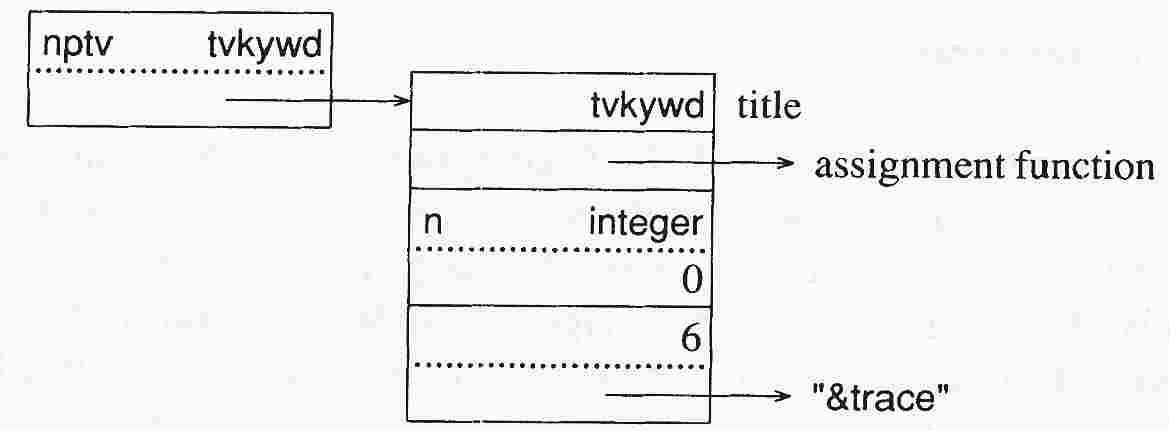
\includegraphics[width=3.9543in,height=1.4398in]{ib-img/ib-img017.jpg} 
%% \begin{picture}(300,120)(-20,0)
%% \put(0,80){\dvboxptr{tvkywd}{nptv}{60}{}}
%% \put(140,64){\blkboxptr{tvkywd}{50}{assignment function}}
%% \put(140,32){\dvbox{integer}{n}{0}}
%% \put(140,0){\dvboxptr{6}{}{50}{"\&trace"}}
%% \end{picture}

It is worth noting that the more conventional approach to handling the
problem of assignment to keywords and other special cases is to compile
special code if the special case occurs an assignment context. It is not
always possible, however, to determine the context in which a variable is
used in Icon. Assume \texttt{tb} is a table and consider a procedure of the form

\begin{iconcode}
\>procedure tabvar(n)\\
\> ...\\
\>return tb[n]\\
\>end
\end{iconcode}

The semantics of Icon dictate that the result returned in this case
should be a variable, not just its value, so that it is possible to
write an expression such as

\iconline{
\>tabvar(5) := 10
}

\noindent
which has the effect of assigning the value 10 to \texttt{tb[5]}.

The translator has no way of knowing that an assignment to the call
\texttt{tabvar(5)} is equivalent to an assignment to \texttt{tb[5]}. In
fact, the translator cannot even determine that the value of
\texttt{tabvar} will be a function when the previous assignment is
performed, much less that it will be the procedure given earlier.
The trapped-variable mechanism provides a way to handle
uniformly all such situations.

\subsection[4.3.2.2 Keyword Variables]{4.3.2.2 Keyword Variables}
Trapped variables are especially useful when dealing with cases where a
variable sometimes needs special treatment and sometimes not. But keywords
{\em always} require special treatment, so they have their own types,
distinct from the everyday numerical and string types. The keyword type
codes are defined symbolically (values for other types are given in
section 4.4.3).

\begin{iconcode}
\#define \>\>\>T\_Kywdint	\>\>\>\>\>\>\>20 \>\>\>\>/* integer keyword */\\
\#define \>\>\>T\_Kywdpos	\>\>\>\>\>\>\>21 \>\>\>\>/* keyword \&pos */\\
\#define \>\>\>T\_Kywdsubj  \>\>\>\>\>\>\>22 \>\>\>\>/* keyword \&subject */\\
\#define \>\>\>T\_Kywdwin	\>\>\>\>\>\>\>23 \>\>\>\>/* keyword \&window */\\
\#define \>\>\>T\_Kywdstr	\>\>\>\>\>\>\>24 \>\>\>\>/* string keyword */\\
\#define \>\>\>T\_Kywdevent \>\>\>\>\>\>\>25 \>\>\>\>/* keyword \&eventsource, etc. */
\end{iconcode}

There are four keyword variables that require special processing for
assignment: \texttt{\&trace}, \texttt{\&random}, \texttt{\&subject},
and \texttt{\&pos}. The keyword \texttt{\&random} is treated in
essentially the same way that \texttt{\&trace} is. Assignment to
\texttt{\&subject} requires a string value and has the side effect of
assigning the value \texttt{1} to \texttt{\&pos}. Assignment to
\texttt{\&pos} is even more complicated: not only must the value
assigned be an integer, but if it is not positive, it must also be
converted to the positive equivalent with respect to the length of
\texttt{\&subject}. In any event, if the value in the assignment to
\texttt{\&pos} is not in the range of \texttt{\&subject}, the
assignment fails. Dereferencing these keywords, on the other hand,
requires no special processing.

See section 12.2 for a further discussion of keyword variables

\section[4.4 Descriptors and Blocks in C]{4.4 Descriptors and Blocks in C}

Descriptors and blocks of data are described and depicted abstractly
in the previous sections of this chapter. In order to understand the
implementation of some aspects of Icon, it is helpful to examine the C
code that actually defines and manipulates data.

The following sections illustrate typical C declarations for the
structures used in the implementation of Icon. Some of the terminology
and operations that appear frequently in the C code are included as
well. Other operations are introduced in subsequent chapters. as they
are needed.

\subsection[4.4.1 Descriptors]{4.4.1 Descriptors}

As mentioned in Sec. 4.1, for C compilers in which ints and pointers
are the same size, the size of a word is the size of an int, while if
pointers are larger than ints, the size of a word is the size of a
long, or a long long. The difference between these models of memory is
handled by typedefs under the control of conditional compilation. Two
constants that characterize the sizes are defined: IntBits and
WordBits. These sizes are used to select appropriate definitions for
signed and unsigned words. The fact that on some 64-bit C compilers a
\texttt{long} is only 32 bits, while on others it is 64 bits,
complicates matters. The symbol \texttt{LongLongWord} indicates this
situation.

\bigskip

% re-insert colors
\begin{iconcode}
\>\#if IntBits != WordBits\\
\>\>{\color{blue}\#ifdef LongLongWord}\\
\>\>\>{\color{blue}typedef long long int word;}\\
\>\>\>{\color{blue}typedef unsigned long long int uword;}\\
\>\>{\color{blue}\#else}\\
\>\>\>typedef long int word;\\
\>\>\>typedef unsigned long uword;\\
\>\>{\color{blue}\#endif}\\
\>\#else \>\>\>\>\>\>\> /* IntBits != WordBits */ \\
\>typedef int word;\\
\>typedef unsigned int uword;\\
\>\#endif
\end{iconcode}

A descriptor is declared as a structure:

\begin{iconcode}
\>struct descrip \{\ \ /* descriptor */\\
\>\>word dword;\ \ /*\ \ type field */\\
\>\>union \{\\
\>\>\>word integr;\ \ /*\ \ integer value */\\
% blue
{\color{blue}\#ifdef DescriptorDouble}\\
\>\>\>{\color{blue}double realval;}\\
{\color{blue}\#endif}\\
\>\>\>char *sptr;\ \ /*\ \ pointer to character string */\\
\>\>\>union block *bptr;\ \ /*\ \ pointer to a block */\\
\>\>\>struct descrip *dptr;\ \ /*\ \ pointer to a descriptor */\\
\>\>\} vword;\\
\>\};
\end{iconcode}

The v-word of a descriptor is a union that reflects its various uses:
an integer, a pointer to a string, a pointer to a block, or a pointer
to another descriptor (in the case of a variable).

\subsection[4.4.2 Blocks]{4.4.2 Blocks}

Each block type has a structure declaration. For example. the
declaration for record blocks is

\begin{iconcode}
\>struct b\_record \{\>\>\>\>\>\>\>\>\> /* record block */\\
\>\>word title;\>\>\>\>\>\>\>\> /*\ T\_Record */\\
\>\>word blksize;\>\>\>\>\>\>\>\> /*\ \ size of block */\\
\>\> word id;\>\>\>\>\>\>\>\> /*\ \ identification number */\\
\>\>union block *recdesc;\>\>\>\>\>\>\>\> /*   pointer to record constructor */\\
\>\>struct descrip fields[1];\>\>\>\>\>\>\>\> /*\ \ fields */\\
\>\};
\end{iconcode}

Blocks for records vary in size, depending on the number of fields
declared for the record type. The size of 1 in

\iconline{
\ \ struct descrip fields[1];
}

\noindent is provided to satisfy the C compiler. Actual blocks for
records are constructed at run time in a region that is managed by
Icon's storage allocator. Such blocks conform to the previous
declaration, but the number of fields varies. The declaration provides
a means of accessing portions of such blocks from C.

The declaration for substring trapped-variable blocks is

\begin{iconcode}
struct b\_tvsubs \{\>\>\>\>\>\>\>\>/* substring trapped variable block */\\
\>word title;\>\>\>\>\>\>\>	    /* T\_Tvsubs */\\
\>word sslen;\>\>\>\>\>\>\>		/* length of substring */\\
\>word sspos;\>\>\>\>\>\>\>		/*  position of substring */\\
\>struct descrip ssvar;\>\>\>\>\>\>\>/* variable that substring is from */\\
\};
\end{iconcode}

Note that the title fields of \texttt{b\_record} and
\texttt{b\_tvsubs} contain type codes, as indicated in previous
diagrams. The second field of \texttt{b\_record} is a size as
mentioned previously, but \texttt{b\_tvsubs} has no size field, since
all substring trapped-variable blocks are the same size, which therefore
can be determined from their type.

The block union given in the declaration of \texttt{struct descrip}
consists of a union of all block types:

\begin{iconcode}
\>union block \{\\
\>\>struct b\_real realblk;\\
\>\>struct b\_cset cset;\\
\>\>struct b\_file file;\\
\>\>struct b\_proc proc;\\
\>\>struct b\_list list;\\
\>\>struct b\_lelem lelem;\\
\>\>struct b\_table table;\\
\>\>struct b\_telem telem;\\
\>\>struct b\_set set;\\
\>\>struct b\_selem selem;\\
\>\>struct b\_record record;\\
\>\>struct b\_tvsubs tvsubs;\\
\>\>struct b\_tvtbl tvtbl;\\
\>\>struct b\_refresh refresh;\\
\>\>struct b\_coexpr coexpr;\\
\>\>struct b\_externl externl;\\
\>\>struct b\_slots slots;\\
\>\>struct b\_bignum bignumblk;\\
\>\};
\end{iconcode}

Note that there are several kinds of blocks in addition to those that
correspond to source-language data types.

\subsection[4.4.3 Defined Constants]{4.4.3 Defined Constants}

The type codes are defined symbolically:

\begin{iconcode}
\#define\>\>\> T\_Null		\>\>\>\>\>0\\	
\#define\>\>\> T\_Integer	\>\>\>\>\>1\\	
\#define\>\>\> T\_Lrgint	\>\>\>\>\>2\\	
\#define\>\>\> T\_Real		\>\>\>\>\>3\\	
\#define\>\>\> T\_Cset		\>\>\>\>\>4\\	
\#define\>\>\> T\_File		\>\>\>\>\>5\\	
\#define\>\>\> T\_Proc		\>\>\>\>\>6\\	
\#define\>\>\> T\_Record	\>\>\>\>\>7\\	
\#define\>\>\> T\_List		\>\>\>\>\>8\\	
\#define\>\>\> T\_Lelem		\>\>\>\>\>9\\	
\#define\>\>\> T\_Set		\>\>\>\>\>10\\
\#define\>\>\> T\_Selem		\>\>\>\>\>11\\
\#define\>\>\> T\_Table		\>\>\>\>\>12\\
\#define\>\>\> T Telem		\>\>\>\>\>13\\
\#define\>\>\> T\_Tvtbl		\>\>\>\>\>14\\
\#define\>\>\> T\_Slots		\>\>\>\>\>15\\
\#define\>\>\> T\_Tvsubs	\>\>\>\>\>16\\
\#define\>\>\> T\_Refresh	\>\>\>\>\>17\\
\#define\>\>\> T\_Coexpr	\>\>\>\>\>18\\
\#define\>\>\> T\_External	\>\>\>\>\>19
\end{iconcode}

The type codes in diagrams are abbreviated, as indicated by previous examples.


The defined constants for d-word flags are

\begin{iconcode}
\>n\>\>F\_Nqual\\
\>p\>\>F\_Ptr\\
\>v\>\>F\_Var\\
\>t\>\>F\_Tvar
\end{iconcode}

The values of these flags depend on the word size of the computer.

The d-words of descriptors are defined in terms of flags and type codes:

\begin{iconcode}
\#define D\_Null	\>\>\>\>\>\>\>\>(T\_Null | F\_Nqual)\\                   
\#define D\_Integer \>\>\>\>\>\>\>\>(T\_Integer | F\_Nqual)\\            	 
\#define D\_Lrgint  \>\>\>\>\>\>\>\>(T\_Lrgint | F\_Ptr | F\_Nqual)\\     	 
\#define D\_Real    \>\>\>\>\>\>\>\>(T\_Real | F\_Ptr | F\_Nqual)\\          
\#define D\_Cset    \>\>\>\>\>\>\>\>(T\_Cset | F\_Ptr | F\_Nqual)\\          
\#define D\_File    \>\>\>\>\>\>\>\>(T\_File | F\_Ptr | F\_Nqual)\\          
\#define D\_Proc    \>\>\>\>\>\>\>\>(T\_Proc | F\_Ptr | F\_Nqual)\\          
\#define D\_List    \>\>\>\>\>\>\>\>(T\_List | F\_Ptr | F\_Nqual)\\          
\#define D\_Table   \>\>\>\>\>\>\>\>(T\_Table | F\_Ptr | F\_Nqual)\\       	 
\#define D\_Set     \>\>\>\>\>\>\>\>(T\_Set | F\_Ptr | F\_Nqual)\\           
\#define D\_Selem   \>\>\>\>\>\>\>\>(T\_Selem | F\_Ptr | F\_Nqual)\\       	 
\#define D\_Record  \>\>\>\>\>\>\>\>(T\_Record | F\_Ptr | F\_Nqual)\\     	 
\#define D\_Telem   \>\>\>\>\>\>\>\>(T\_Telem | F\_Ptr | F\_Nqual)\\       	 
\#define D\_Lelem   \>\>\>\>\>\>\>\>(T\_Lelem | F\_Ptr | F\_Nqual)\\       	 
\#define D\_Tvsubs  \>\>\>\>\>\>\>\>(T\_Tvsubs | D\_Tvar)\\               	 
\#define D\_Tvtbl   \>\>\>\>\>\>\>\>(T Tvtbl | D\_Tvar)\\                  	 
\#define D\_Coexpr  \>\>\>\>\>\>\>\>(T\_Coexpr | F\_Ptr | F\_Nqual)\\     	 
\#define D\_Refresh \>\>\>\>\>\>\>\>(T\_Refresh | F\_Ptr | F\_Nqual)\\   	 
\#define D\_Var     \>\>\>\>\>\>\>\>(F\_Var | F\_Nqual | F\_Ptr)\\   
\#define D\_Tvar    \>\>\>\>\>\>\>\>(D\_Var | F\_Tvar)
\end{iconcode}

As indicated previously, flags, type codes, and d-words are
distinguished by the prefixes \texttt{F\_}, \texttt{T\_}, and
\texttt{D\_}, respectively.

\subsection[4.4.4 RTL Coding]{4.4.4 RTL Coding}

Since the optimizing compiler was introduced in versions 8 and 9 of
Icon, the routines for the run-time system use an extended C syntax
called RTL (for Run-Time Language) that encodes the type information
for arguments and results. Some of these are illustrated by the RTL
function for the Icon operator \texttt{*x}, which produces the size of
\texttt{x}:

\begin{iconcode}
\>operator\{1\} * size(x)\\
\>abstract \{ return integer \}\\
\>type\_case x of \{\\
\>\>string: inline \{ return C\_integer StrLen(x); \}\\
\>\>list: inline \{ return C\_integer BlkD(x,List)->size; \}\\
\>\>table: inline \{ return C\_integer BlkD(x,Table)->size; \}\\
\>\>set: inline \{ return C\_integer BlkD(x,Set)->size; \}\\
\>\>cset: inline \{\\
\>\>\>register word i = BlkD(x,Cset)->size;\\
\>\>\>if (i < 0) i = cssize(\&x);\\
\>\>\>return C\_integer i;\\
\>\>\>\}\\
\>\>...\\
\>\>default: \{\\
\>\>\>\>/*\\
\>\>\>\>\ * Try to convert it to a string.\\
\>\>\>\>\ */\\
\>\>\>\ \ if !cnv:tmp\_string(x) then\\
\>\>\>\>\ \ runerr(112, x);\ \ /* no notion of size */\\
\>\>\>\ \ inline \{\\
\>\>\>\>\ \ return C\_integer StrLen(x);\\
\>\>\>\>\ \ \}\\
\>\>\>\ \ \}\\
\>\>\}\\
end
\end{iconcode}

\texttt{operator} is an RTL construct that performs several
operations. One of these operations is to provide a C function
declaration. Since the function is called by the interpreter, the
header is somewhat different from what it would be if \texttt{size}
were called directly. The details are described in Chapter 8.

The arguments of the Icon operation are referred to via named
descriptors, such as \texttt{x}. The result that is produced is also a
descriptor.

RTL extends C's \texttt{return} statement to include type information,
with which the d-word of the return value is set to
\texttt{D\_lnteger}, since the returned value is a
\texttt{C\_integer}. Next, the \texttt{type\_case} selects different
branches of code depending on the type of x. In the generated code
there is a test to determine if descriptor \texttt{x} holds a
qualifier. \texttt{Qual()} is a macro that is defined as

\iconline{
\>\#define Qual(d)\ \ (!((d).dword \& F\_Nqual))
}

If \texttt{x} is a qualifier, its length is placed in the v-word of
the return value descriptor, using the macros IntVal and StrLen, which
are defined as

\begin{iconcode}
\>\#define IntVal(d)\ \ ((d).vword.integr)\\
\>\#define StrLen(d)\ \ ((d).dword)
\end{iconcode}

If \texttt{x} is not a qualifier, then the size depends on the
type. The macro \texttt{Type()} isolates the type code

\iconline{
\>\#define Type(d)\ \ ((d).dword \& TypeMask)
}

\noindent where the value of \texttt{TypeMask} is 63, providing
considerable room for additions to Icon's internal types.

For most Icon types that are represented by blocks, their
source-language size is contained in their \texttt{size} field. The
macro \texttt{BlkLoc()} accesses a pointer in the v-field of a
descriptor and is defined as

\iconline{
\>\#define BlkLoc(d) ((d).vword.bptr)
}

A more specialized macro \texttt{BlkD()} wraps uses of
\texttt{BlkLoc()} and subsequent union member access, allowing
descriptor-block consistency to be verified at run-time if desired.


If the type is not one of those given, the final task is an attempt to
convert \texttt{x} to a string. The RTL expression
\texttt{cnv:tmp\_string()} does this, using local temporary
buffer. The value of \texttt{x} is changed accordingly. A fixed-sized
buffer can be used, since there is a limit to the size of a string
that can be obtained by converting other types. This limit is 256,
which is reached only for conversion of \texttt{\&cset}. The
conversion may fail, as for \texttt{*\&null}, which is signaled by the
return value 0 from \texttt{cnv:tmp\_string()}. In this case, program
execution is terminated with a run-time: error message, using
\texttt{runerr()}. If the conversion is successful, the size is placed
in the v-word of the result, as is the case if \texttt{x} was a
qualifier originally.

\textsc{Retrospective}: Descriptors provide a uniform way of
representing Icon values and variables. Since descriptors for all
types of data are the same size, there are no problems with assigning
different types of values to a variable---they all fit.

The importance of strings is reflected in the separation of
descriptors into two classes---qualifiers and nonqualifiers---by the \texttt{n}
flag. The advantages of the qualifier representation for strings are
discussed in Chapter 5.

It is comparatively easy to add a new type to Icon. A new type code is
needed to distinguish it from other types. If the possible values of
the new type are small enough to fit into the v-word, as is the case
for integers, no other data is needed. For example, the value of a
character data type could be contained in its descriptor. For types
that have values that are too large to fit into a v-word, pointers to
blocks containing the data are placed in the v-words instead. Lists,
sets, and tables are examples of data types that are represented this
way. See Chapters 6 and 7.

\bigskip

\noindent\textbf{EXERCISES}

\noindent\textbf{4.1} Give examples of Icon programs in which
heterogeneous aggregates are used in significant ways.

\noindent\textbf{4.2} Design a system of type declarations for Icon so
that the translator could do type checking. Give special consideration
to aggregates, especially those that may change in size during program
execution. Do this from two perspectives: (a) changing the semantics
of Icon as little as possible, and (b) maximizing ,the type checking
that can be done by the translator at the expense of flexibility in
programming.

\noindent\textbf{4.3} Suppose that functions in Icon were not
first-class values and that their meanings were bound at translation
time. How much could the translator do in the way of error checking?

\noindent\textbf{4.4} Compile a list of all Icon functions and
operators. Are there any that do not require argument type checking?
Are there any that require type checking but not conversion? Identify
those that are polymorphic. For the polymorphic ones, identify the
different kinds of computations that are performed depending on the
types of the arguments.

\noindent\textbf{4.5} Compose a table of all type checks and
conversions that are required for Icon functions and operators.

\noindent\textbf{4.6} To what extent would the implementation of Icon
be simplified if automatic type conversion were not supported? How
would this affect the programmer?

\noindent\textbf{4.7} Why is it desirable for string qualifiers not to have
flags and for all other kinds of descriptors to have flags indicating they
are not qualifiers, rather than the other way around?

\noindent\textbf{4.8} Is the n flag that distinguishes string qualifiers
from all other descriptors really necessary? If not, explain how to
distinguish the different types of descriptors without this flag.

\noindent\textbf{4.9} On computers with extremely limited address
space, two-word descriptors may be impractically large. Describe how
one-word descriptors might be designed, discuss how various types
might be represented, and describe the ramifications for storage
utilization and execution speed.

\noindent\textbf{4.10} Identify the diagrams in this chapter that
would be different if they were drawn for a computer with 16-bit
words.  Indicate the differences.

\noindent\textbf{4.11} There is nothing in the nature of keywords that
requires them to be processed in a special way for assignment but not
for dereferencing. Invent a new keyword that is a variable that
requires processing when it is dereferenced. Show how to generalize
the keyword trapped-variable mechanism to handle such cases.

\noindent\textbf{4.12} List all the syntactically distinct cases in which the
translator can determine whether a keyword variable is used in an
assignment or dereferencing context.

\noindent\textbf{4.13} What would be gained if special code were compiled for
those cases in which the context for keyword variables could be determined?

\chapter{Strings and Csets}

\textsc{Perspective}: Several aspects of strings as a language feature
in Icon have a strong influence on how they are handled by the
implementation. First of all, strings are the most frequently used
type of data in the majority of Icon programs. The number of different
strings and the total amount of string data often are
large. Therefore, it is important to be able to store and access
strings efficiently.

Icon has many operations on strings---nearly fifty of them. Some
operations, such as determining the size of a string, are performed
frequently. The efficiency of these operations is an important issue
and influences, to a considerable extent, how strings are represented.

Icon strings may be very long. Although some limitation on the maximum
length of a string may be acceptable as a compromise with the
architecture of the computer on which Icon is implemented (and hence
considerations of efficiency), this maximum must be so large as to be
irrelevant for most Icon programs.

String lengths are determined dynamically during program execution,
instead of being specified statically in declarations. Much of the
advantage of string processing in Icon over other programming
languages comes from the automatic management of storage for strings.

Any of the 256 8-bit ASCII characters can appear in an Icon
string. Even the {\textquotedbl}null{\textquotedbl} character is
allowed.

Several operations in Icon return substrings of other
strings. Substrings tend to occur frequently, especially in programs
that analyze (as opposed to synthesize) strings.


Strings in Icon are atomic---there are no operations in Icon that
change the characters in existing strings. This aspect of Icon is not
obvious; in fact, there are operations that appear to change the
characters in strings. The atomic nature of string operations in Icon
simplifies its implementation considerably. For example, assignment of
a string value to a variable need not (and does not) copy the string.

The order in which characters appear is an essential aspect of
strings. There are many situations in Icon, however, where several
characters have the same status but where their order is
irrelevant. For example, the concepts of vowels and punctuation marks
depend on set membership but not on order. Csets are provided for such
situations. Interestingly, many computations can be performed using
csets that have nothing to do with the characters themselves (Griswold
and Griswold 1983, pp. 181-191).


\section[5.1 Strings]{5.1 Strings}
\subsection[5.1.1 Representation of Strings]{5.1.1 Representation of Strings}

Although it may appear natural for the characters of a string to be
stored in consecutive bytes, this has not always been so. On earlier
computer architectures without byte addressing and character
operations, some string-manipulation languages represented strings by
linked lists of words, each word containing a single character. Such a
representation seems bizarre for modem computer architectures and
obviously consumes a very large amount of memory-an intolerable amount
for a language like Icon.

The C programming language represents strings (really arrays of
characters) by successive bytes in memory, using a zero (null) byte to
indicate the end of a string. Consequently, the end of a string can be
determined from the string itself, without any external
information. On the other hand, determining the length of a string, if
it is not already known, requires indexing through it, incrementing a
counter until a null byte is found. Furthermore, and very important
for a language like Icon, substrings (except terminal ones) cannot
occur within strings, since every C string must end with a null byte.

Since any character can occur in an Icon string, it is not possible to
use C's null-termination approach to mark ends of strings. Therefore,
there is no way to detect the end of a string from the string itself,
and there must be some external way to determine where a string
ends. This consideration provides the motivation for the qualifier
representation described in the last chapter. The qualifier provides
information, external to the string itself, that delimits the string
by the address of its first character and its length. Such a
representation makes the computation of substrings fast and
simple---and, of course, determining the length of a string is
fast and independent of its length.

Note that C-style strings serve perfectly well as Icon-style strings;
the null byte at the end of a C-style string can be ignored by
Icon. This allows strings produced by C functions to be used by
Icon. The converse is not true; in order for an Icon string to be used
by C, a copy must be made with a null byte appended at the end.

Some strings are compiled into the run-time system and others, such as
strings that appear as literals in a program, are contained in icode
files that are loaded into memory when program execution
begins. During program execution, Icon strings may be stored in work
areas (usually referred to as
{\textquotedbl}buffers{\textquotedbl}). Most newly created strings,
however, are allocated in a common string region.

As source-language operations construct new strings, their characters
are appended to the end of those already in the string region. The
amount of space allocated in the string region typically increases
during program execution until the region is full, at which point it
is compacted by garbage collection, squeezing out characters that are
no longer needed. See Chapter 11 for details.

In the previous chapter, the string to which a qualifier points is
depicted by an arrow followed by the string. For example, the string
{\textquotedbl}the{\textquotedbl} is represented by the qualifier

\begin{center}
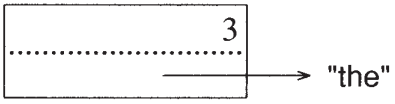
\includegraphics[width=2.1925in,height=0.5598in]{ib-img/ib-img018.png}
\end{center}

The pointer to {\textquotedbl}the{\textquotedbl} is just a notational
convenience. A more accurate representation is

\begin{center}
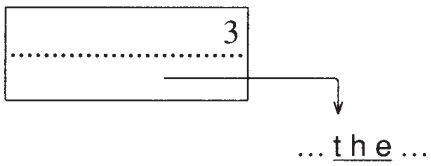
\includegraphics[width=2.3835in,height=0.85in]{ib-img/ib-img019.png}
\end{center}

The actual value of the v-word might be 0x569a (hexadecimal), where
the character t is at memory location 0x569a, the character h is at
location 0x569b, and the character e is at location 0x569c.

\subsection[5.1.2 Concatenation]{5.1.2 Concatenation}

In an expression such as

{\ttfamily\mdseries
\ \ s := {\textquotedbl}hello{\textquotedbl}}

\noindent the string {\textquotedbl}hello{\textquotedbl} is contained
in data provided as part of the icode file, and a qualifier for it is
assigned to s; no string is constructed. Some operations that produce
strings require the allocation of new strings. Concatenation is a
typical example:

{\ttfamily\mdseries
\ \ s1 := {\textquotedbl}ab{\textquotedbl} {\textbar}{\textbar} {\textquotedbl}cdef{\textquotedbl}}

In this expression, the concatenation operation allocates space for
six characters, copies the two strings into this space, and produces a
qualifier for the result:

\begin{center}
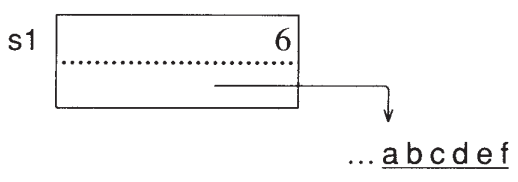
\includegraphics[width=2.6783in,height=0.9366in]{ib-img/ib-img020.png}
\end{center}

This qualifier then becomes the value of \texttt{s1}.

There are important optimizations in concatenation. If the first
argument in a concatenation is the last string in the string region,
the second argument is simply appended to the end of the string
region. Thus, operations of the form

{\ttfamily\mdseries
\ \ s := s {\textbar}{\textbar} \textit{expr}}

\noindent perform less allocation than operations of the form

{\ttfamily\mdseries
\ \ s := \textit{expr }{\textbar}{\textbar} s}

Similarly, if the strings being concatenated are already adjacent, no
concatenation need be performed. Except for these optimizations, no
string construction operation attempts to use another instance of a
string that may exist somewhere else in the string region. As a
result,

{\ttfamily\mdseries
\ \ s1 := {\textquotedbl}ab{\textquotedbl} {\textbar}{\textbar} {\textquotedbl}c{\textquotedbl}\newline
\ \ s2 := {\textquotedbl}a{\textquotedbl} {\textbar}{\textbar} {\textquotedbl}bc{\textquotedbl}}

\noindent produce two distinct strings:

\begin{center}
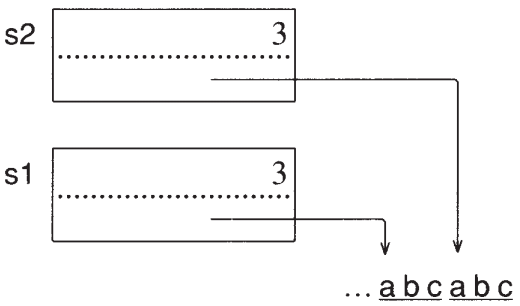
\includegraphics[width=2.4256in,height=1.572in]{ib-img/ib-img021.png}
\end{center}

The RTL code for the concatenation operation is

{\ttfamily\mdseries
\ \ \ operator\{1\} {\textbar}{\textbar} cater(x,y)}

{\ttfamily\mdseries
\ \ \ if !cnv:string(x) then}

{\ttfamily\mdseries
\ \ \ \ \ \ runerr(103, x)}

{\ttfamily\mdseries
\ \ \ if !cnv:string(y) then}

{\ttfamily\mdseries
\ \ \ \ \ \ runerr(103, y)}


\bigskip

{\ttfamily\mdseries
\ \ \ abstract \{}

{\ttfamily\mdseries
\ \ \ \ \ \ return string}

{\ttfamily\mdseries
\ \ \ \ \ \ \}}

{\ttfamily\mdseries
\ \ \ body \{}

{\ttfamily\mdseries
\ \ \ \ \ \ CURTSTATE();}


\bigskip

{\ttfamily\mdseries
\ \ \ \ \ \ /*}

{\ttfamily\mdseries
\ \ \ \ \ \ \ * \ Optimization 1: \ The strings to be concatenated are}

{\ttfamily\mdseries
\ \ \ \ \ \ \ * \ already adjacent in memory; no allocation is required.}

{\ttfamily\mdseries
\ \ \ \ \ \ \ */}

{\ttfamily\mdseries
\ \ \ \ \ \ if (StrLoc(x) + StrLen(x) == StrLoc(y)) \{}

{\ttfamily\mdseries
\ \ \ \ \ \ \ \ \ StrLoc(result) = StrLoc(x);}

{\ttfamily\mdseries
\ \ \ \ \ \ \ \ \ StrLen(result) = StrLen(x) + StrLen(y);}

{\ttfamily\mdseries
\ \ \ \ \ \ \ \ \ return result;}

{\ttfamily\mdseries
\ \ \ \ \ \ \ \ \ \}}

{\ttfamily\mdseries
\ \ \ \ \ \ else if ((StrLoc(x) + StrLen(x) == strfree)}

{\ttfamily\mdseries
\ \ \ \ \ \ \&\& (DiffPtrs(strend,strfree) {\textgreater} StrLen(y))) \{}

{\ttfamily\mdseries
\ \ \ \ \ \ \ \ \ /*}

{\ttfamily\mdseries
\ \ \ \ \ \ \ \ \ \ * Optimization 2: The end of x is at the end of the string space.}

{\ttfamily\mdseries
\ \ \ \ \ \ \ \ \ \ * \ Hence, x was the last string allocated and need}

{\ttfamily\mdseries
\ \ \ \ \ \ \ \ \ \ * \ not be re-allocated. y is appended to the string}

{\ttfamily\mdseries
\ \ \ \ \ \ \ \ \ \ * \ space and the result is pointed to the start of x.}

{\ttfamily\mdseries
\ \ \ \ \ \ \ \ \ \ */}

{\ttfamily\mdseries
\ \  result = x;}

{\ttfamily\mdseries
\ \  /*}

{\ttfamily\mdseries
\ \  \ * Append y to the end of the string space.}

{\ttfamily\mdseries
\ \  \ */}

{\ttfamily\mdseries
\ \  Protect(alcstr(StrLoc(y),StrLen(y)), runerr(0));}

{\ttfamily\mdseries
\ \  /*}

{\ttfamily\mdseries
\ \  \ * \ Set the length of the result and return.}

{\ttfamily\mdseries
\ \  \ */}

{\ttfamily\mdseries
\ \  StrLen(result) = StrLen(x) + StrLen(y);}

{\ttfamily\mdseries
\ \  return result;}

{\ttfamily\mdseries
\ \ \ \ \ \ \ \ \ \}}


\bigskip

{\ttfamily\mdseries
\ \ \ \ \ \ /*}

{\ttfamily\mdseries
\ \ \ \ \ \ \ * Otherwise, allocate space for x and y, and copy them}

{\ttfamily\mdseries
\ \ \ \ \ \ \ * \ to the end of the string space.}

{\ttfamily\mdseries
\ \ \ \ \ \ \ */}

{\ttfamily\mdseries
\ \ \ \ \ \ Protect(StrLoc(result) = alcstr(NULL, StrLen(x) +}

{\ttfamily\mdseries
\ \ \ \ \ \ \ \ \ \ \ \ \ \ \ \ \ \ \ \ \ \ \ \ \ \ \ \ \ \ \ \ \ \ \ \ \ \ \ \ \ StrLen(y)), runerr(0));}

{\ttfamily\mdseries
\ \ \ \ \ \ memcpy(StrLoc(result), StrLoc(x), StrLen(x));}

{\ttfamily\mdseries
\ \ \ \ \ \ memcpy(StrLoc(result) + StrLen(x), StrLoc(y), StrLen(y));}


\bigskip

{\ttfamily\mdseries
\ \ \ \ \ \ /*}

{\ttfamily\mdseries
\ \ \ \ \ \ \ * \ Set the length of the result and return.}

{\ttfamily\mdseries
\ \ \ \ \ \ \ */}

{\ttfamily\mdseries
\ \ \ \ \ \ StrLen(result) = StrLen(x) + StrLen(y);}

{\ttfamily\mdseries
\ \ \ \ \ \ return result;}

{\ttfamily
\ \ \ \ \ \ \}}

{\ttfamily
end}


The function \texttt{strreq(n)} assures that there are at least
\texttt{n} bytes available in the allocated string region. See Chapter
11 for details. The function \texttt{alcstr(s, n)} allocates
\texttt{n} characters and copies \texttt{s} to that space. The global
variable \texttt{strfree} points to the beginning of the free space at
the end of the allocated string region.

\subsection[5.1.3 Substrings]{5.1.3 Substrings}

Many string operations do not require the allocation of a new string
but only produce new qualifiers. For example, if the value of
\texttt{s1} is \texttt{{\textquotedbl}abcdef{\textquotedbl}}, the
substring formed by

{\ttfamily\mdseries
\ \ \ s2 := s1[3:6]}

\noindent does not allocate a new string but only produces a qualifier
that points to a substring of \texttt{s1}:



\begin{center}
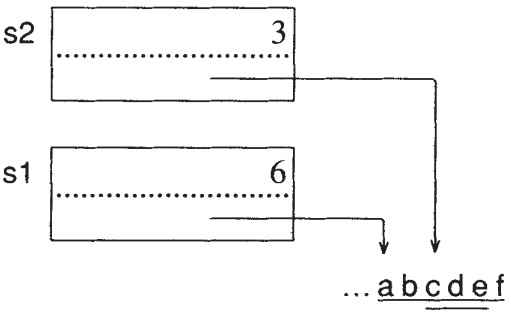
\includegraphics[width=2.3339in,height=1.5516in]{ib-img/ib-img022.png}
\end{center}

In order for Icon string values to be represented in memory by
substrings, it is essential that there be no Icon operation that
changes the characters inside a string. As mentioned earlier, this is
the case, although it is not obvious from a cursory examination of the
language. C, on the other hand, allows the characters in a string to
be changed. The difference is that C considers a string to be an array
of characters and allows assignment to the elements of the array,
while Icon considers a string to be an indivisible atomic object. It
makes no more sense in Icon to try to change a character in a string
than it does to try to change a digit in an integer. Thus, if

{\ttfamily\mdseries
\ \ \ i := j}

and

{\ttfamily\mdseries
\ \ \ j := j + 1}

\noindent the value of \texttt{i} does not change as a result of the
subsequent assignment to \texttt{j}. So it is with strings in Icon.

Admittedly, there are operations in Icon that \textit{appear }to
change the characters in a string. For example,

{\ttfamily\mdseries
\ \ \ s1[3] := {\textquotedbl}x{\textquotedbl}}

\noindent gives the appearance of changing the third character in
\texttt{s1} to \texttt{{\textquotedbl}x{\textquotedbl}}.  However,
this expression is simply shorthand for

{\ttfamily\mdseries
\ \ \ s1 := s1[1:3] {\textbar}{\textbar} {\textquotedbl}x{\textquotedbl} {\textbar}{\textbar} s1[4:0]}

A new string is created by concatenation and a new qualifier for it is
assigned to \texttt{s1}, as shown by

\ \  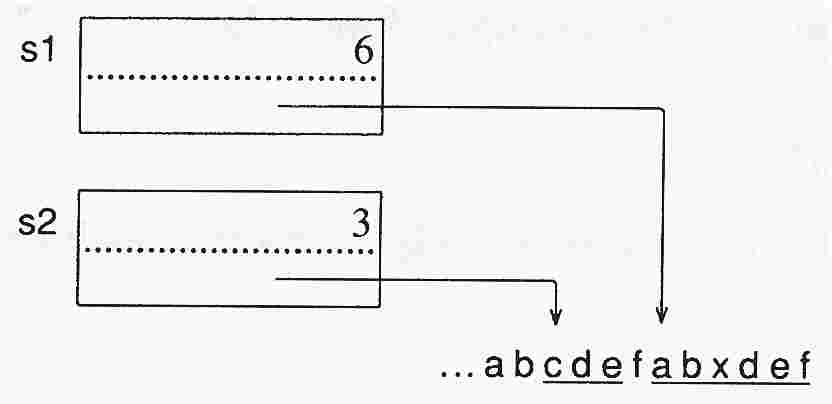
\includegraphics[width=2.778in,height=1.3484in]{ib-img/ib-img023.jpg} 

Of course, the length of the string may be increased or decreased by
assignment to a substring, as in

\ \ \ s1[3] := {\textquotedbl}xxx{\textquotedbl}

\ \ \ s1 [2:5] := {\textquotedbl}{\textquotedbl}

\subsection[5.1.4 Assignment to Subscripted Strings]{5.1.4 Assignment to Subscripted Strings}

Expressions such as \texttt{x[i]} and \texttt{x[i:j]} represent a
particular challenge in the implementation of Icon. In the first
place, the translator cannot determine the type of x. In the case of
\texttt{x[i]}, there are four basic types that \texttt{x} may
legitimately have: string, list, table, and record. Of course, any
type that can be converted to a string is legitimate
also. Unfortunately, the \textit{nature }of the operation, not just
the details of its implementation, depends on the type. For strings,

{\ttfamily\mdseries
\ \ \ s1 [3] := s2}

\noindent replaces the third character of \texttt{s1} by \texttt{s2}
and is equivalent to concatenation, as described previously.  For
lists, tables, and records,

{\ttfamily\mdseries
\ \ \ x[3] := y}

\noindent changes the third \textit{element }of \texttt{x} to
\texttt{y}{}--quite a different matter (see Exercise 5.5).

This problem is pervasive in Icon and only needs to be noted in
passing here. The more serious problem is that even if the subscripted
variable is a string, the subscripting expression has different
meanings, depending on the context in which it appears.

If \texttt{s} is a variable, then \texttt{s[i]} and \texttt{s[i:j]}
also are variables. In a dereferencing context, such as

{\ttfamily\mdseries
\ \ \ write(s[2:5])}

\noindent the result produced by \texttt{s[2:5]} is simply a substring
of \texttt{s}, and the subscripting expression produces the
appropriate qualifier.

Assignment to a subscripted string, as in

{\ttfamily\mdseries
\ \ \ s[2:5] := {\textquotedbl}xxx{\textquotedbl}}

\noindent is not at all what it appears to be superficially. Instead,
as already noted, it shorthand for an assignment to \texttt{s}:

{\ttfamily\mdseries
\ \ \ s := s[1] {\textbar}{\textbar} {\textquotedbl}xxx{\textquotedbl} {\textbar}{\textbar} s[6:0]}

If the translator could determine whether a subscripting expression is
used in dereferencing or assignment context, it could produce
different code for the two cases. As mentioned in Sec. 4.3.2, however,
the translator cannot always make this determination. Consequently,
trapped variables are used for subscripted string much in the way they
are used for keywords. For example, if the value of \texttt{s} is
\texttt{{\textquotedbl}abcdef{\textquotedbl}}, the result of
evaluating the subscripting expression \texttt{s[2:5]} is a
\textit{substring trapped variable} that has the form


\ \  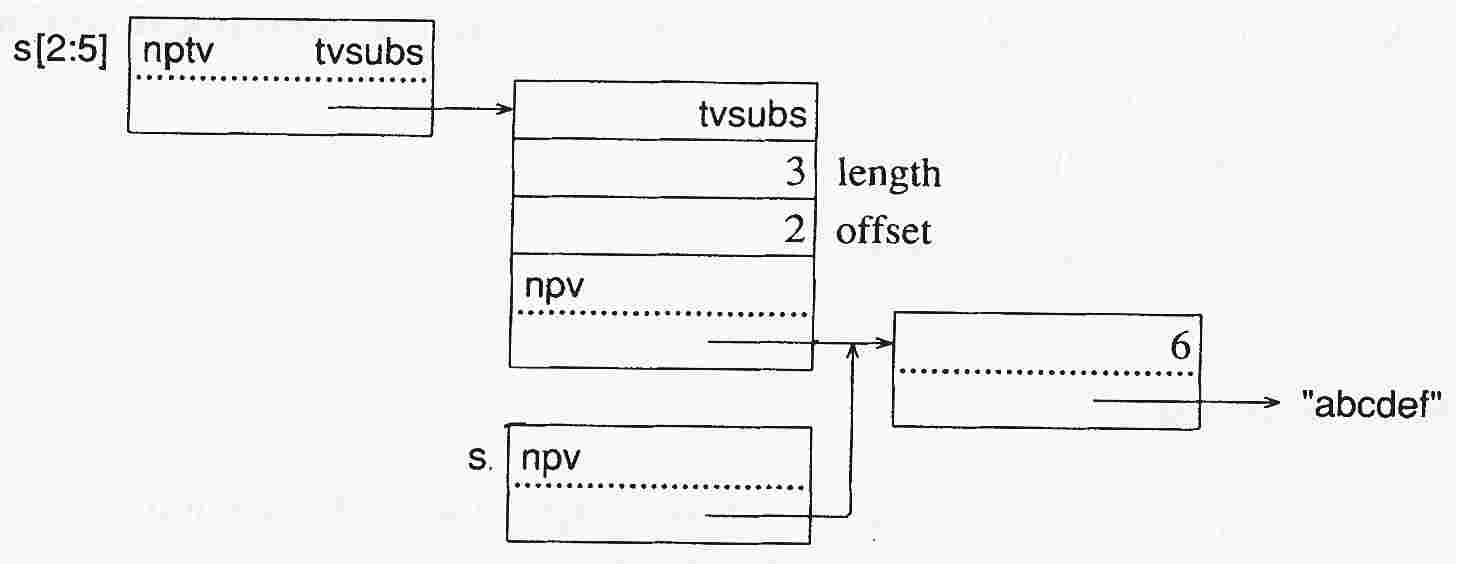
\includegraphics[width=4.9161in,height=1.8835in]{ib-img/ib-img024.jpg} 


Note that both the variable for \texttt{s} and the variable in the
substring trapped-variable block point to the same value. This makes
it possible for assignment to the substring trapped variable to change
the value of \texttt{s}.

The length and offset of the substring provide the necessary
information either to produce a qualifier for the substring, in case
the subscripting expression is dereferenced, or to construct a new
string in case an assignment is made to the subscripting
expression. For example, after an assignment such as

{\ttfamily\mdseries
\ \ \ s[2:5] := {\textquotedbl}x{\textquotedbl}}

\noindent the situation is

\ \  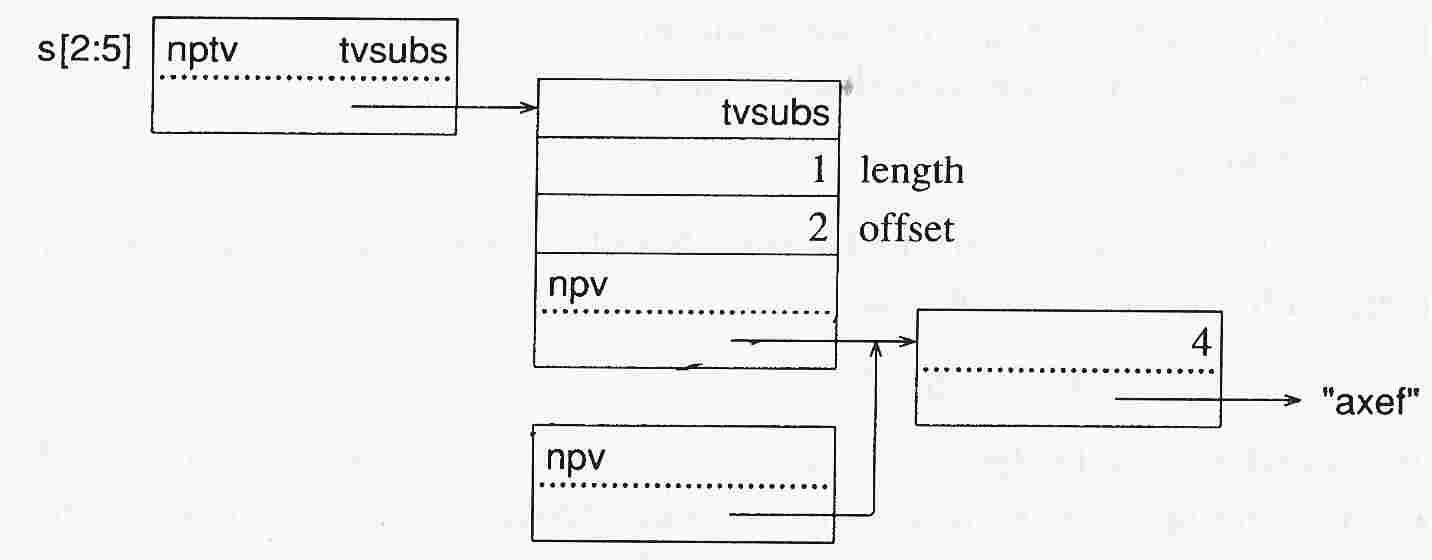
\includegraphics[width=4.8098in,height=1.8693in]{ib-img/ib-img025.jpg} 

Note that the value of \texttt{s} has changed. The length of the
subscripted portion of the string has been changed to correspond to
the length of the string assigned to it. This reflects the fact that
subscripting identifies the portions of the string before and after
the subscripted portion (\texttt{{\textquotedbl}a{\textquotedbl}} and
\texttt{{\textquotedbl}ef{\textquotedbl}}, in this case). In the case
of a multiple assignment to a subscripted string, only the original
subscripted portion is changed. Thus, in

{\ttfamily
\ \ \ (s[2:5] := {\textquotedbl}x{\textquotedbl}) := \textit{{\textquotedbl}yyyyy{\textquotedbl}}}

\noindent the final value of \texttt{s} is
\texttt{{\textquotedbl}ayyyyyef{\textquotedbl}}.

\subsection[5.1.5 Mapping]{5.1.5 Mapping}

String mapping is interesting in its own right, and the RTL function
that implements it illustrates several aspects of string processing:

{\ttfamily\mdseries
function\{1\} map(s1,s2,s3)}

{\ttfamily\mdseries
\ \ \ /*}

{\ttfamily\mdseries
\ \ \ \ * s1 must be a string; s2 and s3 default to (string }

{\ttfamily\mdseries
\ \ \ \ * conversions of) \&ucase and \&lcase, respectively.}

{\ttfamily\mdseries
\ \ \ \ */}

{\ttfamily\mdseries
\ \ \ if !cnv:string(s1) then}

{\ttfamily\mdseries
\ \ \ \ \ \ runerr(103,s1)}

{\ttfamily\mdseries
\ \ \ ...}

{\ttfamily\mdseries
\ \ \ abstract \{}

{\ttfamily\mdseries
\ \ \ \ \ \ return string}

{\ttfamily\mdseries
\ \ \ \ \ \ \}}

{\ttfamily\mdseries
\ \ \ body \{}

{\ttfamily\mdseries
\ \ \ \ \ \ register int i;}

{\ttfamily\mdseries
\ \ \ \ \ \ register word slen;}

{\ttfamily\mdseries
\ \ \ \ \ \ register char *str1, *str2, *str3;}

{\ttfamily\mdseries
\#ifndef Concurrent}

{\ttfamily\mdseries
\ \ \ \ \ \ static char maptab[256];}

{\ttfamily\mdseries
\#endif\ \ \ \ \ \ \ \ \ \ /* Concurrent */}

{\ttfamily\mdseries
\ \ \ \ \ \ CURTSTATE();}


\ \ \ \ \ \ /*


\ \ \ \ \ \ \ * Default is here, conversion only if cached maptab fails


\ \ \ \ \ \ \ */


\ \ \ \ \ \ if (is:null(s2))


\ \ \ \ \ \ \ \ \ s2 = ucase;


\ \ \ \ \ \ /*


\ \ \ \ \ \ \ * Short-cut conversions of \&lcase and \&ucase.


\ \ \ \ \ \ \ */


\ \ \ \ \ \ else \{


\ \  struct descrip \_k\_lcase\_, \_k\_ucase\_;


\ \  Klcase(\&\_k\_lcase\_);


\ \  Kucase(\&\_k\_ucase\_);


\ \  if (s2.dword == D\_Cset) \{


\ \  \ \ \ if (BlkLoc(s2) == BlkLoc(\_k\_lcase\_)) \{


\ \  \ \ \ \ \ \ s2 = lcase;


\ \  \ \ \ \ \ \ \}


\ \  \ \ \ else if (BlkLoc(s2) == BlkLoc(\_k\_ucase\_)) \{


\ \  \ \ \ \ \ \ s2 = ucase;


\ \  \ \ \ \ \ \ \}


\ \  \ \ \ \}


\ \  \}


\bigskip


\ \ \ \ \ \ if (is:null(s3))


\ \ \ \ \ \ \ \ \ s3 = lcase;


\ \ \ \ \ \ /*


\ \ \ \ \ \ \ * Short-cut conversions of \&lcase and \&ucase.


\ \ \ \ \ \ \ */


\ \ \ \ \ \ else \{


\ \  struct descrip \_k\_lcase\_, \_k\_ucase\_;


\ \  Klcase(\&\_k\_lcase\_);


\ \  Kucase(\&\_k\_ucase\_);


\ \  if (s3.dword == D\_Cset) \{


\ \  \ \ \ if (BlkLoc(s3) == BlkLoc(\_k\_lcase\_)) \{


\ \  \ \ \ \ \ \ s3 = lcase;


\ \  \ \ \ \ \ \ \}


\ \  \ \ \ else if (BlkLoc(s3) == BlkLoc(\_k\_ucase\_)) \{


\ \  \ \ \ \ \ \ s3 = ucase;


\ \  \ \ \ \ \ \ \}


\ \  \ \ \ \}


\ \  \}


\#endif\ \ \ \ \ \ \ \ \ \ /* !COMPILER */


\bigskip


\ \ \ \ \ \ /*


\ \ \ \ \ \ \ * If s2 and s3 are the same as for the last call of map,


\ \ \ \ \ \ \ * \ the current values in maptab can be used. Otherwise, the


\ \ \ \ \ \ \ * \ mapping information must be recomputed.


\ \ \ \ \ \ \ */


\ \ \ \ \ \ if (!EqlDesc(maps2,s2) {\textbar}{\textbar} !EqlDesc(maps3,s3)) \{


\ \ \ \ \ \ \ \ \ maps2 = s2;


\ \ \ \ \ \ \ \ \ maps3 = s3;


\bigskip


\#if !COMPILER


\ \ \ \ \ \ \ \ \ if (!cnv:string(s2,s2))


\ \ \ \ \ \ \ \ \ \ \ \ runerr(103,s2);


\ \ \ \ \ \ \ \ \ if (!cnv:string(s3,s3))


\ \ \ \ \ \ \ \ \ \ \ \ runerr(103,s3);


\#endif\ \ \ \ \ \ \ \ \ \ /* !COMPILER */


\ \ \ \ \ \ \ \ \ /*


\ \ \ \ \ \ \ \ \ \ * s2 and s3 must be of the same length


\ \ \ \ \ \ \ \ \ \ */


\ \ \ \ \ \ \ \ \ if (StrLen(s2) != StrLen(s3))


\ \ \ \ \ \ \ \ \ \ \ \ runerr(208);


\bigskip


\ \ \ \ \ \ \ \ \ /*


\ \ \ \ \ \ \ \ \ \ * The array maptab is used to perform the mapping. \ First,


\ \ \ \ \ \ \ \ \ \ * \ maptab[i] is initialized with i for i from 0 to 255.


\ \ \ \ \ \ \ \ \ \ * \ Then, for each character in s2, the position in maptab


\ \ \ \ \ \ \ \ \ \ * \ corresponding to the value of the character is assigned


\ \ \ \ \ \ \ \ \ \ * \ the value of the character in s3 that is in the same


\ \ \ \ \ \ \ \ \ \ * \ position as the character from s2.


\ \ \ \ \ \ \ \ \ \ */


\ \ \ \ \ \ \ \ \ str2 = StrLoc(s2);


\ \ \ \ \ \ \ \ \ str3 = StrLoc(s3);


\ \ \ \ \ \ \ \ \ for (i = 0; i {\textless}= 255; i++)


\ \ \ \ \ \ \ \ \ \ \ \ maptab[i] = i;


\ \ \ \ \ \ \ \ \ for (slen = 0; slen {\textless} StrLen(s2); slen++)


\ \ \ \ \ \ \ \ \ \ \ \ maptab[str2[slen]\&0377] = str3[slen];


\ \ \ \ \ \ \ \ \ \}


\bigskip


\ \ \ \ \ \ slen = StrLen(s1);


\bigskip


\ \ \ \ \ \ if (slen == 0) \{


\ \  return emptystr;


\ \  \}


\ \ \ \ \ \ else if (slen == 1) \{


\ \  char c = maptab[*(StrLoc(s1)) \& 0xFF];


\ \  return string(1, (char *)\&allchars[FromAscii(c) \& 0xFF]);


\ \  \}


\bigskip


\ \ \ \ \ \ /*


\ \ \ \ \ \ \ * The result is a string the size of s1; create the result


\ \ \ \ \ \ \ * \ string, but specify no value for it.


\ \ \ \ \ \ \ */


\ \ \ \ \ \ StrLen(result) = slen;


\ \ \ \ \ \ Protect(StrLoc(result) = alcstr(NULL, slen), runerr(0));


\ \ \ \ \ \ str1 = StrLoc(s1);


\ \ \ \ \ \ str2 = StrLoc(result);


\bigskip


\ \ \ \ \ \ /*


\ \ \ \ \ \ \ * Run through the string, using values in maptab to do the


\ \ \ \ \ \ \ * \ mapping.


\ \ \ \ \ \ \ */


\ \ \ \ \ \ while (slen-{}- {\textgreater} 0)


\ \ \ \ \ \ \ \ \ *str2++ = maptab[(*str1++)\&0377];


\bigskip


\ \ \ \ \ \ return result;


\ \ \ \ \ \ \}


end


\bigskip


The mapping is done using the character array \texttt{maptab}. This
array is set up by first assigning every possible character to its own
position in \texttt{maptab} and then replacing the characters at
positions corresponding to characters in \texttt{s2} by the
corresponding characters in \texttt{s3}. Note that if a character
occurs more than once in \texttt{s2}, its last (rightmost)
correspondence with a character in \texttt{s3} applies.

To avoid rebuilding \texttt{maptab} unnecessarily, this step is
bypassed if \texttt{map()} is called with the same values of
\texttt{s2} and \texttt{s3} as in the previous call. The global
variabIes \texttt{maps2} and \texttt{maps3} are used to hold these
{\textquotedbl}cached{\textquotedbl} values. The macro
\texttt{EqlDesc(d1,d2)} tests the equivalence of the descriptors
\texttt{d1} and \texttt{d2}.

The function \texttt{map()} is an example of a function that defaults
null-valued arguments. Omitted arguments are supplied as null
values. The defaults for \texttt{s2} and \texttt{s3} are
\texttt{\&ucase} and \texttt{\&lcase}, respectively. Consequently,

{\ttfamily\mdseries
\ \ map(s)}

\noindent
is equivalent to

{\ttfamily\mdseries
\ \ map(s, \&ucase, \&lcase)}


The macro \texttt{ChkNull(d)} tests whether or not \texttt{d} is
null. The values of \texttt{\&ucase} and \texttt{\&lcase} are in the
global constants \texttt{ucase} and \texttt{lcase}.

\section{Csets}

Since Icon uses 8-bit characters, regardless of the computer on which
it is implemented, there are 256 different characters that can occur
in csets. A cset block consists of the usual title containing the cset
type code followed by a word that contains the number of characters in
the cset. Next, there are words containing a total of 256 bits. Each
bit represents one character, with a bit value of 1 indicating that
the character is present in the cset and a bit value of 0 indicating
it is absent. An example is the value of the keyword \texttt{\&ascii}:


\ \  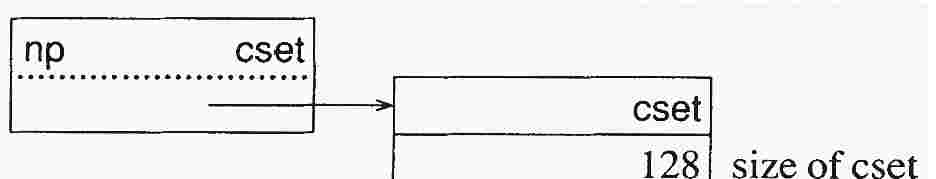
\includegraphics[width=3.2063in,height=0.5965in]{ib-img/ib-img026.jpg} 


The first 128 bits are 1, since these are the bits that correspond to
those in ASCII character set.

The C structure for a cset block is

{\ttfamily\mdseries
\ \ \ struct b\_cset \{\ \ \ \ \ \ \ \ /* cset block */}

{\ttfamily\mdseries
\ \ \ \ \ \ word title;\ \ \ \ \ \ \ \ /*\ \ T\_Cset */}

{\ttfamily\mdseries
\ \ \ \ \ \ word size;\ \ \ \ \ \ \ \ /*\ \ size of cset */}

{\ttfamily\mdseries
\ \ \ \ \ \ unsigned int bits [CsetSize];\ \ /*\ \ array of bits */}

{\ttfamily\mdseries
\ \ \ \};}

\noindent where CsetSize is the number of words required to make up a
total of 256 bits. CsetSize is 8 on a computer with 32-bit words and 4
on a computer with 64-bit words.

Cset operations are comparatively straightforward. The characters in a
cset are represented by a bit vector that is divided into words to
accommodate conventional computer architectures. For example, the C
code for cset complementation is

{\ttfamily\mdseries
operator\{1\} \~{} compl(x)}

{\ttfamily\mdseries
\ \ \ /*}

{\ttfamily\mdseries
\ \ \ \ * x must be a cset.}

{\ttfamily\mdseries
\ \ \ \ */}

{\ttfamily\mdseries
\ \ \ if !cnv:tmp\_cset(x) then}

{\ttfamily\mdseries
\ \ \ \ \ \ runerr(104, x)}


\bigskip

{\ttfamily\mdseries
\ \ \ abstract \{}

{\ttfamily\mdseries
\ \ \ \ \ \ return cset}

{\ttfamily\mdseries
\ \ \ \ \ \ \}}

{\ttfamily\mdseries
\ \ \ body \{}

{\ttfamily\mdseries
\ \ \ \ \ \ register int i;}

{\ttfamily\mdseries
\ \ \ \ \ \ struct b\_cset *cp, *cpx;}


\bigskip

{\ttfamily\mdseries
\ \ \ \ \ \ /*}

{\ttfamily\mdseries
\ \ \ \ \ \ \ * Allocate a new cset and then copy each cset word from}

{\ttfamily\mdseries
\ \ \ \ \ \ \ * \ x into the new cset words, complementing each bit.}

{\ttfamily\mdseries
\ \ \ \ \ \ \ */}

{\ttfamily\mdseries
\ \ \ \ \ \ Protect(cp = alccset(), runerr(0));}

{\ttfamily\mdseries
\ \ \ \ \ \ /* must come after alccset() since BlkLoc(x) could move */}

{\ttfamily\mdseries
\ \ \ \ \ \ cpx = (struct b\_cset *)BlkLoc(x); }

{\ttfamily\mdseries
\ \ \ \ \ \ for (i = 0; i {\textless} CsetSize; i++) }

{\ttfamily\mdseries
\ \ \ \ \ \ \ \ \ \ cp-{\textgreater}bits[i] = \~{}cpx-{\textgreater}bits[i];}

{\ttfamily\mdseries
\ \ \ \ \ \ return cset(cp);}

{\ttfamily\mdseries
\ \ \ \ \ \ \}}

{\ttfamily\mdseries
end}


\textsc{Retrospective}: The central role of strings in Icon and the
nature of the operations performed on them leads to a representation
of string data that is distinct from other data. The qualifier
representation is particularly important in providing direct access to
string length and in allowing the construction of substrings without
the allocation of additional storage. The penalty paid is that a
separate test must be performed to distinguish strings from all other
kinds of values.

The ability to assign to subscripted strings causes serious
implementation problems. The trapped-variable mechanism provides a
solution, but it does so at considerable expense in the complexity of
code in the run-time system as well as storage allocation for
trapped-variable blocks. This expense is incurred even if assignment
is not made to a subscripted string.

{\sffamily\bfseries
EXERCISES}

\liststyleLv
\begin{enumerate}
\item \begin{enumerate}

\item What are the ramifications of Icon's use of the 256-bit ASCII
character set, regardless of the {\textquotedbl}native{\textquotedbl}
character set of the computer on which Icon is implemented?

\item Catalog all the operations on strings in Icon and point out any
that might cause special implementation problems.  Indicate the
aspects of strings and string operations in Icon that are the most
important in terms of memory requirements and processing speed.

\item List all the operations in Icon that require the allocation of
space for the construction of strings.

\item It has been suggested that it would be worth trying to avoid
duplicate allocation of the same string by searching the string region
for a newly created string to see if it already exists before
allocating the space for it. Evaluate this proposal.

\item 
Consider the following four expressions:\newline
\texttt{ s1 [i] := s2\newline
 s1 [i+:1] := s2\newline
 a1 [i] := a2\newline
 a1 [i+:1] := a2}\newline
where \texttt{s1} and \texttt{s2} have string values and \texttt{a1}
and \texttt{a2} have list values. Describe the essential differences
between the string and list cases. Explain why these differences
indicate flaws in language design. Suggest an alternative.

\item The substring trapped-variable concept has the advantage of
making it possible to handle all the contexts in which
string-subscripting expressions can occur. It is expensive, however,
in terms of storage utilization. Analyze the impact of this feature on
the performance of {\textquotedbl}typical{\textquotedbl} Icon
programs.

\item Since the contexts in which most subscripting expressions occur
can be determined, describe how to handle these without using trapped
variables.

\item If a subscripting expression is applied to a result that is not
a variable, it is erroneous to use such an expression in an assignment
context. In what situations can the translator detect this error? Are
there any situations in which a subscripting expression is applied to
a variable but in which the expression cannot be used in an assignment
context?

\item There are some potential advantages to unifying the keyword and
substring trapped-variable mechanisms into a single mechanism in which
all trapped variables would have pointers to functions for
dereferencing and assignment. What are the disadvantages of such a
unification?

\item Presumably, it is unlikely for a programmer to have a
constructive need for the polymorphic aspect of subscripting
expressions. Or is it? If it is unlikely, provide a supporting
argument. On the other hand, if there are situations in which this
capability is useful, describe them and give examples.

\item In some uses of \texttt{map(s1, s2, s3)}, \texttt{s1} and
\texttt{s2} remain fixed while \texttt{s3} varies (Griswold
1980b). Devise a heuristic that takes advantage of such usage.

\end{enumerate}
\end{enumerate}

\chapter{Lists}

\textsc{Perspective}:Most programming languages support some form of
vector or array data type in which elements can be referenced by
position. Icon's list data type fills this need, but it differs from
similar types in many languages in that Icon lists are constructed
during program execution instead of being declared during
compilation. Therefore, the size of a list may not be known until run
time.

Icon's lists are data objects. They can be assigned to variables and
passed as arguments to functions. They are not copied when this is
done; in fact, a value of type list is simply a descriptor that points
to the structure that contains the list elements. These aspects of
lists are shared by several other Icon data types and do not add
anything new to the implementation. The attribute of lists that
presents the most challenging implementation problem is their ability
to grow and shrink by the use of stack and queue access mechanisms.

Lists present different faces to the programmer, depending on how they
are used. They may be static vectors referenced by position or they
may be dynamic changing stacks or queues. It might seem that having a
data structure with such apparently discordant access mechanisms would
be awkward and undesirable. In practice, Icon's lists provide a
remarkably flexible mechanism for dealing with many common programming
problems. The two ways of manipulating lists are rarely
intermixed. When both aspects are needed, they usually are needed at
different times. For example, the number of elements needed in a list
often is not known when the list is created. Such a list can be
created with no elements, and the elements can be pushed onto it as
they are produced. Once such a list has been constructed, it may be
accessed by position with no further change in its size.

\section{Structures for Lists}

The fusion of vector, stack, and queue organizations is reflected in
the implementation of Icon by relatively complicated structures that
are designed to provide a reasonable compromise between the
conflicting requirements of the different access mechanisms.


A list consists of a fixed-size \textit{list-header block}, which
contains the usual title, the current size of the list (the number of
elements in it), and block pointers that point to the first and last
blocks on a doubly-linked chain of \textit{list-element blocks} that
contain the actual list elements. List-element blocks vary in size.


A list-element block contains the usual title, the size of the block
in bytes, three words used to determine the locations of elements in
the list-element block and block pointers that point to the next and
previous list-element blocks, if any. A null pointer
\textcolor[rgb]{0.0,0.2784314,1.0}{(in Unicon, a pointer back to the
list header block)} indicates the absence of a pointer to another
list-element block. Following this data, there are slots for
elements. Slots always contain valid descriptors, even if they are not
used to hold list elements.


The structure declarations for list-header blocks and list-element blocks are

\begin{iconcode}
\>struct b\_list \{\>\>\>\>\>\>\>/* list-header block */\\
\>\>word title;\>\>\>\>\>\>\>/*\ \ T\_List */\\
\>\>word size;\>\>\>\>\>\>\>/*\ \ current list size */\\
\>\>word id;\>\>\>\>\>\>\>/*\ \ identification number */\\
\>\>union block *listhead;\>\>\>\>\>\>\>/* first list-element block \textit{*}/\\
\>\>union block *listtail;\>\>\>\>\>\>\>/* last list-element block \textit{*}/\\
\>\};\\
\>struct b\_lelem \{\>\>\>\>\>\>\>/* list-element block */\\
\>\>word title;\>\>\>\>\>\>\>/*\ \ T\_Lelem */\\
\>\>word blksize;\>\>\>\>\>\>\>/*\ \ size of block */\\
\>\>word nslots;\>\>\>\>\>\>\>/*\ \ total number of slots */\\
\>\>word first;\>\>\>\>\>\>\>/*\ \ index of first used slot */\\
\>\>word nused;\>\>\>\>\>\>\>/*\ \ number of used slots */\\
\>\>union block *listprev;\>\>\>\>\>\>\>/* previous list-element block */\\
\>\>union block *listnext;\>\>\>\>\>\>\>/* next list-element block */\\
\>\>struct descrip lslots[1];\>\>\>\>\>\>\>/* array of slots */\\
\>\};
\end{iconcode}

When a list is created, either by

\iconline{
\>list(n, x)
}

\noindent or by

\iconline{
\>[x1 ,x2, ..., xn]
}

\noindent there is only one list-element block. Other list-element
blocks may be added to the chain as the result of pushs or puts.

List-element blocks have a minimum number of slots. This allows some
expansion room for adding elements to lists, such as the empty list, that
are small initially. The minimum number of slots is given by
\texttt{MinListSlots}, which normally is eight. In the examples that
follow, the value of \texttt{MinListSlots} is assumed to be four in order
to keep the diagrams to a manageable size.

The code for the list function is

\begin{iconcode}
function\{1\} list(n, x)\\
\>if is:set(n) then \{\\
\>\>abstract \{\\
\>\>\>return new list(store[type(n).set\_elem])\\
\>\>\ \  \}\\
\>\>body \{\\
\>\>\>struct descrip d;\\
\>\>\>cnv\_list(\&n, \&d); /* can't fail, we know n is a set */\\
\>\>\>return d;\\
\>\>\>\}\\
\>\>\}\\
\>else \{\\
\>\>if !def:C\_integer(n, 0L) then\\
\ \  runerr(101, n)\\
\\
\>abstract \{\\
\>\>return new list(type(x))\\
\>\>\}\\
\\
\>\>tended struct b\_list *hp;\\
\>\>register word i, size;\\
\>\>word nslots;\\
\>\>register struct b\_lelem *bp; /* doesnt need to be tended */\\
\\
\>\>nslots = size = n;\\
\\
\>\>/*\\
\>\>\ * Ensure that the size is positive and that the\\
\>\>\ * \ list-element block has at least MinListSlots slots.\\
\>\>\ */\\
\>\>if (size < 0) \{\\
\>\>\>irunerr(205, n);\\
\>\>\>errorfail;\\
\>\>\>\}\\
\>\>if (nslots == 0)\\
\>\>\>nslots = MinListSlots;\\
\>\>/*\\
\>\>\ * Allocate the list-header block and a list-element block.\\
\>\>\ * \ nslots is the number of slots in the list-element\\
\>\>\ * \ block while size is the number of elements in the list.\\
\>\>\ */\\
\>\>Protect(hp = alclist\_raw(size, nslots), runerr(0));\\
\>\>bp = (struct b\_lelem *)hp->listhead;\\
\\
\>\>/*\\
\>\>\ * Initialize each slot.\\
\>\>\ */\\
\>\>for (i = 0; i < size; i++)\\
\>\>\>bp->lslots[i] = x;\\
\\
\>\>Desc\_EVValD(hp, E\_Lcreate, D\_List);\\
\\
\>\>/*\\
\>\>\ * Return the new list.\\
\>\>\ */\\
\>\>return list(hp);\\
\>\>\}\\
\>\}\\
end
\end{iconcode}

The data structures produced for a list are illustrated by the result
of evaluating

\iconline{
\>a := list(1, 4)
}

\noindent which produces a one-element list containing the value 4:

\noindent
\begin{picture}(420,360)
%\put(0,0){\graphpaper{42}{36}}
\put(130,0){\dvbox{null}{n}{0}}
\put(130,0){\trboxlabel{slot 3}}
\put(130,32){\dvbox{null}{n}{0}}
\put(130,32){\trboxlabel{slot 2}}
\put(130,64){\dvbox{null}{n}{0}}
\put(130,64){\trboxlabel{slot 1}}
\put(130,96){\dvbox{integer}{n}{4}}
\put(130,96){\trboxlabel{slot 0}}
\put(130,128){\nullptrbox{next list-element block}}
{\color{blue}
\put(-10,136){\parbox{100pt}{Unicon replaces the null pointer used by Icon
    with a pointer to the list header block.}}
\multiput(100,136)(4,0){30}{\line(1,0){2}}
\put(370,136){\line(1,0){50}}
\put(420,136){\line(0,1){214}}
\put(420,350){\vector(-1,0){150}}
\put(270,350){\line(-1,0){154}}
\put(116,350){\vector(0,-1){22}}
}
\put(130,144){\nullptrbox{previous list-element block}}
\begin{picture}(0,0)(0,32)
\put(130,192){\blkbox{0}{1}}
\put(130,192){\rightboxlabels{first slot used}{number of slots used}}
\put(130,224){\blkbox{60}{4}}
\put(130,224){\rightboxlabels{size of block}{number of slots in block}}
\put(130,256){\wordbox{lelem}{}}
\put(130,288){\blkbox{}{}}
\put(130,288){\rightboxlabels{first list-element block (head)}
   {last list-element block(tail)}}
\put(130,306){\lptr{40}}
\put(130,288){\lptr{40}}
\put(110,314){\line(0,-1){51}}
\put(110,263){\vector(1,0){20}}
\put(130,320){\wordbox{\textit{id}}{}}
\put(130,336){\blkbox{list}{1}}
\put(130,336){\brboxlabel{number of elements in the list}}
\put(0,352){\dvboxptr{list}{np}{50}{}}
\end{picture}
\end{picture}

\ \ \ \ Data Structures for \texttt{list(1,4)}

Note that there is only one list-element block and that the slot
indexing in the block is zero-based. Unused slots contain null values
that are logically inaccessible.

\section{Queue and Stack Access}

Elements in a list-element block are stored as a doubly-linked
circular queue. If an element is added to the end of the list
\texttt{a}, as in

\iconline{
\>put(a, 5)
}

\noindent the elements of the list are 4 and 5. The value is added to
the '{\textquotedbl}end{\textquotedbl} of the last list-element block,
assuming there is an unused slot (as there is in this case). The code
in \texttt{put()} to do this is

\begin{iconcode}
\>/*\\
\>\ * Point hp to the list-header block and bp to the last\\
\>\ * list-element block.\\
\>\ */\\
\>hp = (struct b\_list *)BlkLoc(x);\\
\>bp = (struct b\_lelem *) hp->listtail;\\
\>/*\\
\>\ * If the last list-element block is full, allocate a new\\
\>\ *\ \ list-element block, make it the first list-element block,\\
\>\ *\ \ and make it the next block of the former last list-element\\
\>\ * block.\\
\>\ */\\
\>if (bp->nused >= bp->nslots) \{\\
\>\>/*\\
\>\>\ * Set i to the size of block to allocate.\\
\>\>\ */\\
\>\>i = hp->size / two;\\
\>\>if (i < MinListSlots)\\\ \  \ \ \ \ \ \ i = MinListSlots;\\
\#ifdef MaxListSlots\\
\>\>if (i > MaxListSlots)\\
\>\>\>i = MaxListSlots;\\
\#endif\ \ \ \ \ \ \ \ \ \ /* MaxListSlots */\\
\>\ \ /*\\
\>\>* Allocate a new list element block. \ If the block\\
\>\>* \ can't be allocated, try smaller blocks.\\
\>\>*/\\
\>\>while ((bp = alclstb(i, (word)0, (word)0)) == NULL) \{\\
\>\>\>i /= 4;\\
\>\>\>if (i < MinListSlots)\\
\>\>\>\>runerr(0);\\
\>\>\}\\
\\
\>\>hp->listtail->lelem.listnext = (union block *) bp;\\
\>\>bp->listprev = hp->listtail;\\
\>\>hp->listtail = (union block *) bp;\\
\>\}\\
\>/*\\
\>\ * Set i to position of new last element and assign val to\\
\>\ * that element.\\
\>\ */\\
\>i = bp->first + bp->nused;\\
\>if (i >= bp->nslots)\\
\>\>i -= bp->nslots;\\
\>bp->lslots[i] = dp[val];\\
\\
\> /*\\
\> \ * Adjust block usage count and current list size.\\
\> \ */\\
\> bp->nused++;\\
\> hp->size++;\\
\> \}\\
\\
\>\>/*\\
\>\>\ * Return the list.\\
\>\>\ */\\
\>\>return x;\\
\>\>\}\\
end
\end{iconcode}

The effect on the list-header block and list-element block is:

\begin{picture}(300,310)(0,32)
\begin{picture}(0,0)(0,-32)
\put(130,0){\dvbox{null}{n}{0}}
\put(130,0){\trboxlabel{slot 3}}
\put(130,32){\dvbox{null}{n}{0}}
\put(130,32){\trboxlabel{slot 2}}
\put(130,64){\dvbox{integer}{n}{5}}
\put(130,64){\trboxlabel{slot 1}}
\put(130,96){\dvbox{integer}{n}{4}}
\put(130,96){\trboxlabel{slot 0}}
\end{picture}
\put(130,160){\nullptrbox{next list-element block}}
\put(130,176){\nullptrbox{previous list-element block}}
\put(130,192){\blkbox{0}{2}}
\put(130,192){\rightboxlabels{first slot used}{number of slots used}}
\put(130,224){\blkbox{60}{4}}
\put(130,224){\rightboxlabels{size of block}{number of slots in block}}
\put(130,256){\wordbox{lelem}{}}
%
\put(0,240){\leftboxlabels{head}{tail}}
\put(0,240){\wordbox{}{}}
\put(0,240){\ruptr{36}{16}}
\put(0,256){\wordboxptr{50}{}}
\put(0,272){\wordbox{\textit{id}}{}}
\put(0,288){\blkbox{list}{2}}
\put(0,288){\brboxlabel{number of elements in the list}}
{\color{blue}
\put(366,168){\line(1,0){60}}
\put(426,168){\line(0,1){160}}
\put(426,328){\vector(-1,0){130}}
\put(296,328){\line(-1,0){316}}
\put(-20,328){\line(0,-1){16}}
\put(-20,312){\vector(1,0){20}}
\multiput(130,168)(4,0){23}{\line(1,0){2}}
\put(130,160){\blboxlabel{(Unicon) pointer to list header}}
}
\end{picture}

\ \ \ \ The List Element-Block after a put

Note that the increase in the number of elements in the header block
and in the number of slots used in the list-element block.

If an element is added to the beginning of a list, as in

\iconline{
\>push(a,3)
}

\noindent the elements of the list are 3, 4, and 5. The new element is
put at the '{\textquotedbl}beginning{\textquotedbl} of the first
list-element block. The result is

\begin{picture}(300,310)(0,32)
\begin{picture}(0,0)(0,-32)
\put(130,0){\dvbox{integer}{n}{3}}
\put(130,0){\trboxlabel{slot 3}}
\put(130,32){\dvbox{null}{n}{0}}
\put(130,32){\trboxlabel{slot 2}}
\put(130,64){\dvbox{integer}{n}{5}}
\put(130,64){\trboxlabel{slot 1}}
\put(130,96){\dvbox{integer}{n}{4}}
\put(130,96){\trboxlabel{slot 0}}
\end{picture}
\put(130,160){\nullptrbox{next list-element block}}
\put(130,176){\nullptrbox{previous list-element block}}
\put(130,192){\blkbox{3}{3}}
\put(130,192){\rightboxlabels{first slot used}{number of slots used}}
\put(130,224){\blkbox{60}{4}}
\put(130,224){\rightboxlabels{size of block}{number of slots in block}}
\put(130,256){\wordbox{lelem}{}}
%
\put(0,240){\leftboxlabels{head}{tail}}
\put(0,240){\wordbox{}{}}
\put(0,240){\ruptr{36}{16}}
\put(0,256){\wordboxptr{50}{}}
\put(0,272){\wordbox{\textit{id}}{}}
\put(0,288){\blkbox{list}{3}}
\put(0,288){\brboxlabel{number of elements in the list}}
{\color{blue}
\put(366,168){\line(1,0){60}}
\put(426,168){\line(0,1){160}}
\put(426,328){\vector(-1,0){130}}
\put(296,328){\line(-1,0){316}}
\put(-20,328){\line(0,-1){16}}
\put(-20,312){\vector(1,0){20}}
\multiput(126,168)(4,0){23}{\line(1,0){2}}
\put(126,160){\blboxlabel{(Unicon) pointer to list header}}
}
\end{picture}

\ \ \ \ The List Element-Block after a push

Note that the {\textquotedbl}beginning,{\textquotedbl} which is before
the first physical slot in the list-element block, is the last
physical slot. The locations of elements that are in a list-element
block are determined by the three integers at the head of the list
element block. {\textquotedbl}Removal{\textquotedbl} of an element by
a pop, get, or pull does not shorten the list-element block or
overwrite the element; the element merely becomes inaccessible.

If an element is added to a list and no more slots are available in the
appropriate list-element block, a new list-element block is allocated and
linked in. The size of the new block is half the number of elements in the
entire list before expansion or \texttt{MinListSlots}, whichever is
greater.
{\color{blue} Unicon also imposes an upper limit of \texttt{MaxListSlots}
on the size of the new block.}
However, if there is not enough memory to allocate a list-element
block of the desired size, the size is reduced to fit into available
memory. For example, following evaluation of

\iconline{
\>push(a,2)
}

\iconline{
\>push(a,1)
}

\noindent the list elements are 1,2,3,4, and 5. The resulting structures are


\begin{picture}(300,520)
%\put(0,0){\graphpaper{30}{52}}
%
\put(0,256){% The top list block
\begin{picture}(300,300)
\put(130,0){\dvbox{integer}{n}{1}}
\put(130,0){\trboxlabel{slot 3}}
\put(130,32){\dvbox{null}{n}{0}}
\put(130,32){\trboxlabel{slot 2}}
\put(130,64){\dvbox{null}{n}{0}}
\put(130,64){\trboxlabel{slot 1}}
\put(130,96){\dvbox{null}{n}{0}}
\put(130,96){\trboxlabel{slot 0}}
\put(130,128){\wordbox{}{}}
\put(130,128){\brboxlabel{next list-element block}}
\put(130,128){\lptr{38}}
\put(130,144){\nullptrbox{previous list-element block}}
\put(130,160){\blkbox{3}{1}}
\put(130,160){\rightboxlabels{first slot used}{number of slots used}}
\put(130,192){\blkbox{60}{4}}
\put(130,192){\rightboxlabels{size of block}{number of slots in block}}
\put(130,224){\wordbox{lelem}{}}
%
\put(0,160){\leftboxlabels{head}{tail}}
\put(0,160){\wordbox{}{}}
\put(0,176){\wordbox{}{}}
\put(0,176){\ruptr{32}{16}}
\put(112,200){\line(0,1){32}}
\put(112,232){\vector(1,0){18}}
\put(0,192){\wordbox{\textit{id}}{}}
\put(0,208){\blkbox{list}{5}}
\put(0,160){\rdptr{32}{100}}
\put(112,68){\line(0,-1){68}}
\put(414,0){\line(0,1){252}}
\put(414,252){\vector(-1,0){100}}
\put(314,252){\line(-1,0){202}}
\put(112,252){\line(0,-1){20}}
{\color{blue}
\put(-44,0){\line(0,1){232}}
\put(-44,232){\vector(1,0){44}}
}
\end{picture}
}
\put(0,0){% The bottom list block
\begin{picture}(300,370)
\put(130,0){\dvbox{integer}{n}{3}}
\put(130,0){\trboxlabel{slot 3}}
\put(130,32){\dvbox{integer}{n}{2}}
\put(130,32){\trboxlabel{slot 2}}
\put(130,64){\dvbox{integer}{n}{5}}
\put(130,64){\trboxlabel{slot 1}}
\put(130,96){\dvbox{integer}{n}{4}}
\put(130,96){\trboxlabel{slot 0}}
\put(130,128){\nullptrbox{next list-element block}}
\put(310,144){\ruptr{24}{104}}
\put(130,144){\wordboxptr{30}{previous list-element block}}
\put(130,160){\blkbox{2}{4}}
\put(130,160){\rightboxlabels{first slot used}{number of slots used}}
\put(130,192){\blkbox{60}{4}}
\put(130,192){\rightboxlabels{size of block}{number of slots in block}}
\put(130,224){\wordbox{lelem}{}}
\put(112,232){\line(0,1){24}}
\put(112,232){\vector(1,0){18}}
{\color{blue}
\put(140,128){\luptr{204}{120}}
\put(120,144){\makebox(0,0)[r]{(Unicon) pointer to list header}}
}
\end{picture}
}
\end{picture}


\ \ The Addition of a List-Element Block


As elements are removed from a list by pop (which is synonymous with
get) or pull. The indices in the appropriate list-element block are
adjusted. The code for pop is

\begin{iconcode}
int c\_get(hp, res)\\
struct b\_list *hp;\\
struct descrip *res;\\
\{\\
\>register word i;\\
\>register struct b\_lelem *bp;\\
\\
\>/*\\
\>\ * Fail if the list is empty.\\
\>\ */\\
\>if (hp->size <= 0)\\
\>\>return 0;\\
\\
\>/*\\
\>\ * Point bp at the first list block. \ If the first block has\\
\>\ * \ no elements in use, point bp at the next list block.\\
\>\ */\\
\>bp = (struct b\_lelem *) hp->listhead;\\
\>if (bp->nused <= 0) \{\\
\>\>bp = (struct b\_lelem *) bp->listnext;\\
\>\>hp->listhead = (union block *) bp;\\
\>\>bp->listprev = NULL;\\
\>\>\}\\
\\
\>/*\\
\>\ * Locate first element and assign it to result for return.\\
\>\ */\\
\>i = bp->first;\\
\>*res = bp->lslots[i];\\
\\
\>/*\\
\>\ * Set bp->first to new first element, or 0 if the block is\\
\>\ * \ now empty. \ Decrement the usage count for the block and\\
\>\ * \ the size of the list.\\
\>\ */\\
\>if (++i >= bp->nslots)\\
\>\>i = 0;\\
\>bp->first = i;\\
\>bp->nused-{}-;\\
\>hp->size-{}-;\\
\>return 1;\\
\}
\end{iconcode}

\noindent where the \texttt{c\_get()} helper function is invoked from RTL as follows:

\begin{iconcode}
function\{0,1\} get\_or\_pop(x)\\
\>if !is:list(x) then\\
\>\>runerr(108, x)\\
\\
\>abstract \{\\
\>\>return store[type(x).lst\_elem]\\
\>\>\}\\
\\
\>body \{\\
\>\>if (!c\_get((struct b\_list *)BlkLoc(x), \&result)) fail;\\
\>\>return result;\\
\>\>\}\\
end
\end{iconcode}

Thus, as a result of

\iconline{
\>pop(a)
}

\noindent
the list elements are 2, 3, 4, and 5. The resulting structures are


\begin{picture}(300,520)
%\put(0,0){\graphpaper{30}{52}}
%
\put(0,256){% The top list block
\begin{picture}(300,300)
\put(130,0){\dvbox{integer}{n}{1}}
\put(130,0){\trboxlabel{slot 3}}
\put(130,32){\dvbox{null}{n}{0}}
\put(130,32){\trboxlabel{slot 2}}
\put(130,64){\dvbox{null}{n}{0}}
\put(130,64){\trboxlabel{slot 1}}
\put(130,96){\dvbox{null}{n}{0}}
\put(130,96){\trboxlabel{slot 0}}
\put(130,128){\wordbox{}{}}
\put(130,128){\brboxlabel{next list-element block}}
\put(130,128){\lptr{38}}
\put(130,144){\nullptrbox{previous list-element block}}
\put(130,160){\blkbox{0}{0}}
\put(130,160){\rightboxlabels{first slot used}{number of slots used}}
\put(130,192){\blkbox{60}{4}}
\put(130,192){\rightboxlabels{size of block}{number of slots in block}}
\put(130,224){\wordbox{lelem}{}}
%
\put(0,160){\leftboxlabels{head}{tail}}
\put(0,160){\wordbox{}{}}
\put(0,176){\wordbox{}{}}
\put(0,176){\ruptr{32}{16}}
\put(112,200){\line(0,1){32}}
\put(112,232){\vector(1,0){18}}
\put(0,192){\wordbox{\textit{id}}{}}
\put(0,208){\blkbox{list}{4}}
\put(0,160){\rdptr{32}{100}}
\put(112,68){\line(0,-1){68}}
\put(414,0){\line(0,1){252}}
\put(414,252){\vector(-1,0){100}}
\put(314,252){\line(-1,0){202}}
\put(112,252){\line(0,-1){20}}
{\color{blue}
\put(-44,0){\line(0,1){232}}
\put(-44,232){\vector(1,0){44}}
}
\end{picture}
}
\put(0,0){% The bottom list block
\begin{picture}(300,370)
\put(130,0){\dvbox{integer}{n}{3}}
\put(130,0){\trboxlabel{slot 3}}
\put(130,32){\dvbox{integer}{n}{2}}
\put(130,32){\trboxlabel{slot 2}}
\put(130,64){\dvbox{integer}{n}{5}}
\put(130,64){\trboxlabel{slot 1}}
\put(130,96){\dvbox{integer}{n}{4}}
\put(130,96){\trboxlabel{slot 0}}
\put(130,128){\nullptrbox{next list-element block}}
\put(310,144){\ruptr{24}{104}}
\put(130,144){\wordboxptr{30}{previous list-element block}}
\put(130,160){\blkbox{2}{4}}
\put(130,160){\rightboxlabels{first slot used}{number of slots used}}
\put(130,192){\blkbox{60}{4}}
\put(130,192){\rightboxlabels{size of block}{number of slots in block}}
\put(130,224){\wordbox{lelem}{}}
\put(112,232){\line(0,1){24}}
\put(112,232){\vector(1,0){18}}
{\color{blue}
\put(140,128){\luptr{204}{120}}
\put(120,144){\makebox(0,0)[r]{(Unicon) pointer to list header}}
}
\end{picture}
}
\end{picture}

\ \ \ \ The Result of Removing Elements from a List-Element Block


Note that the first list-element block is still linked in the chain,
even though it no longer contains any elements that are logically
accessible. A list-element block is not removed from the chain when it
becomes empty. It is removed only when an element is removed from a
list that already has an empty list-element block. Thus, there is
always at least one list-element block on the chain, even if the list
is empty. Aside from simplifying the access to list-element blocks
from the list-header block, this strategy avoids repeated allocation
in the case that pop/push pairs occur at the boundary of two
list-element blocks.

Continuing the previous example,

\iconline{
\>pop(a)
}

\noindent leaves the list elements 3, 4, and 5. The empty list-element
block is removed from the chain:

\begin{picture}(300,310)(-20,0)
\put(130,0){\dvbox{integer}{n}{3}}
\put(130,0){\trboxlabel{slot 3}}
\put(130,32){\dvbox{integer}{n}{2}}
\put(130,32){\trboxlabel{slot 2}}
\put(130,64){\dvbox{integer}{n}{5}}
\put(130,64){\trboxlabel{slot 1}}
\put(130,96){\dvbox{integer}{n}{4}}
\put(130,96){\trboxlabel{slot 0}}
\put(130,128){\nullptrbox{next list-element block}}
\put(130,144){\nullptrbox{previous list-element block}}
%% \put(130,128){\dvbox{null}{n}{0}}
%% \put(130,128){\trboxlabel{next list-element block}}
%% \put(130,160){\dvbox{null}{n}{0}}
%% \put(130,160){\trboxlabel{previous list-element block}}

\put(130,160){\blkbox{3}{3}}
\put(130,160){\rightboxlabels{first slot used}{number of slots used}}
\put(130,192){\blkbox{60}{4}}
\put(130,192){\rightboxlabels{size of block}{number of slots in block}}
\put(130,224){\wordbox{lelem}{}}
%
\put(0,208){\leftboxlabels{head}{tail}}
\put(0,208){\wordbox{}{}}
\put(0,208){\ruptr{36}{16}}
\put(0,224){\wordboxptr{50}{}}
\put(0,240){\wordbox{\textit{id}}{}}
\put(0,256){\blkbox{list}{3}}
\put(0,256){\brboxlabel{number of elements in the list}}
{\color{blue}
\put(138,128){\luptr{200}{40}}
\put(-42,176){\line(0,1){104}}
\put(-42,280){\vector(1,0){42}}
\put(120,144){\makebox(0,0)[r]{(Unicon) pointer to list header}}
}
\end{picture}

\ \ Removal of an Empty List-Element Block

Note that the value 2 is still physically in the list-element block,
although it is logically inaccessible.

\section{Positional Access}

Positional reference of the form \texttt{a[i]} requires locating the
correct list-element block. Out-of-range references can be determined
by examining the list-header block. If the list has several
list-element blocks, this involves linking through the list-element
blocks, while keeping track of the count of elements in each block
until the appropriate one is reached. The result of evaluating
\texttt{a[i]} is a variable that points to the appropriate slot.

The portion of the subscripting code that handles lists is

\begin{iconcode}
\>type\_case dx of \{\\
\>\>list: \{\\
\>\>\>abstract \{\\
\>\>\>\>return type(dx).lst\_elem\\
\>\>\>\>\}\\
\>\>\>/*\\
\>\>\>\ * Make sure that y is a C integer.\\
\>\>\>\ */\\
\>\>\>if !cnv:C\_integer(y) then \{\\
\>\>/*\\
\>\>\ * If it isn't a C integer, but is a large integer,\\
\>\>\ * fail on the out-of-range index.\\
\>\>\ */\\
\>\>if cnv : integer(y) then inline \{ fail; \}\\
\>\>runerr(101, y)\\
\>\>\}\\
\>\>\>body \{\\
\>\>\>\>word i, j;\\
\>\>\>\>register union block *bp; /* no need to be tended */\\
\>\>\>\>struct b\_list *lp; \ \ \ /* doesn't need to be tended */\\
\\
\>\>/*\\
\>\>\ * Make sure that subscript y is in range.\\
\>\>\ */\\
\>\>\>\>lp = (struct b\_list *)BlkLoc(dx);\\
\>\>\>\>i = cvpos((long)y, (long)lp->size);\\
\>\>\>\>if (i == CvtFail || i > lp->size)\\
\>\>\>\>\>fail;\\
\>\>\>\>/*\\
\>\>\>\>\ * Locate the list-element block containing the\\
\>\>\>\>\ * \ desired element.\\
\>\>\>\>\ */\\
\>\>\>\>bp = lp->listhead;\\
\>\>\>\>j = 1;\\
\>\>/*\\
\>\>\ * y is in range, so bp can never be null here. If it\\
\>\>\ * was, a memory violation would occur in the code that\\
\>\>\ * follows, anyhow, so exiting the loop on a NULL bp\\
\>\>\ * makes no sense.\\
\>\>\ */\\
\>\ \ while (i >= j + bp->lelem.nused) \{\\
\>\>\ \ j += bp->lelem.nused;\\
\>\>\ \ bp = BlkLoc(bp->lelem.listnext);\\
\>\>\ \ \}\\
\\
\>\>/*\\
\>\>* Locate desired element and return a pointer to it.\\
\>\>*/\\
\>\>i += bp->lelem.first - j;\\
\>\>if (i >= bp->lelem.nslots)\\
\>\>\>i -= bp->lelem.nslots;\\
\>\>return struct\_var(\&bp->lelem.lslots[i], bp);\\
\>\>\}\\
\>\}
\end{iconcode}

For the preceding example, \texttt{a[3]} produces a variable that
points indirectly to the descriptor for the value 5:

\begin{picture}(300,250)(-20,0)
\put(140,0){\dvbox{integer}{n}{3}}
\put(140,0){\trboxlabel{slot 3}}
\put(140,32){\dvbox{integer}{n}{2}}
\put(140,32){\trboxlabel{slot 2}}
\put(140,64){\dvbox{integer}{n}{5}}
\put(140,64){\trboxlabel{slot 1}}
\put(140,96){\dvbox{integer}{n}{4}}
\put(140,96){\trboxlabel{slot 0}}
\put(140,128){\nullptrbox{next list-element block}}
\put(140,144){\nullptrbox{previous list-element block}}
\put(140,160){\blkbox{3}{3}}
\put(140,160){\rightboxlabels{first slot used}{number of slots used}}
\put(140,192){\blkbox{60}{4}}
\put(140,192){\rightboxlabels{size of block}{number of slots in block}}
\put(140,224){\wordbox{lelem}{}}
%
\put(0,80){\dvboxptr{9}{npv}{40}{}}
\put(120,88){\line(0,1){144}}
\put(120,232){\vector(1,0){20}}
\multiput(120,88)(4,0){4}{\line(1,0){2}}
\put(136,88){\vector(1,0){4}}
{\color{blue}
\multiput(126,136)(4,0){26}{\line(1,0){2}}
\put(126,128){\blboxlabel{(Unicon) pointer to list header}}
}
\end{picture}

\ \ \ \ Referencing a List Element

Note the offset of nine words in the d-word of the variable.  In version 6 of
Icon the descriptor pointed directly at the variable and the offset enabled the
garbage collector to locate the top of the block. In current versions of Icon
and Unicon the variable points to the top of the block and the offset enables
the correct list-element to be referenced. This change was necessitated by the
introduction of block pointers --- see Chapter 11 for details.

\section{Arrays (Unicon only)}

The Unicon language provides a special case of the general list structure
that is optimized for fast access to the list-elements. An array is a list
where all the list-elements are the same numeric type and are in a single
block. It is created by calling

\iconline{array($dimen$, $value$)}

\noindent which will return a one dimensional ``vector'' of $dimen$
elements that are all set to $value$.  $value$ may be a small integer or
a floating point value. It may also be a list, in which case the value for
the array is the value of the first element of the list.

%% [DonW] To check (in the source):
%% What happens when a descriptor is needed (eg. a procedure returns an
%% integer value that may be assigned to)?
%%        A descriptor is built by calling struct_var
%% What happens when a real value is assigned to an integer array and vice-versa?
%%        The code for the assignment operator checks the type of the header block
%%        to see if it's an array. If so it converts the array to a list of the
%%        type changes.
%% What do array slices do?
%%
%% Does the garbage collector need to know about arrays? I suspect yes
%%        No special treatment is required for arrays
%% What happens if an assignment is made beyond the end of the array?
%%        It should fail, but strange things happen.

For example, following evaluation of

\iconline{vec := array(100,42)}

\noindent 
there will be 100 integers in the array, all set to 42.
The resulting structures are

\begin{picture}(400,260)(0,-10)
\begin{picture}(0,0)(-145,0)
\put(120,0){\blkbox{42}{42}}
\put(129,0){\blboxlabel{\texttt{vec[100]}}}
\put(129,0){\tlboxlabel{\texttt{vec[99]}}}
\put(120,0){\upetc}
\put(100,50){\vdots}
\put(120,80){\downetc}
\put(120,80){\blkbox{42}{42}}
\put(120,80){\tlboxlabel{\texttt{vec[1]}}}
\put(120,80){\blboxlabel{\texttt{vec[2]}}}
\put(120,112){\nullptrbox{dims}}
\put(120,128){\wordbox{}{}}
\put(115,184){\makebox(100,0)[l]{First (and only) list-element block}}
\put(120,144){\blkbox{intarray}{416}}
\put(120,144){\brboxlabel{size (bytes)}}
\end{picture}
\put(130,232){\makebox(108,0){List header block}}
\put(130,144){\nullptrbox{}}
\put(130,160){\blkboxptr{\textit{id}}{55}{}}
\put(130,192){\blkbox{list}{100}}
\put(-5,208){\dvboxptr{list}{npv}{54}{}}
\put(-5,208){\tlboxlabel{\texttt{vec}}}
\put(450,216){\vector(-1,0){219}}
\put(450,216){\line(0,-1){80}}
\put(450,136){\line(-1,0){100}}
\end{picture}

At present (January 2017) multi-dimensional arrays are not supported,
although there is provision in the data structures for more than one
dimension. Multi dimensional arrays will be created by calling

\iconline{array($dimen_1$, $dimen_2$, \dots , $dimen_n$, $value$)}

The only change to the diagram above will be that the null pointer in the
\texttt{dims} field will be replaced by a pointer to another intarray block
that contains each of the values $dimen_1$ \dots $dimen_n$.

Provided that the elements in the array are only assigned values of the
same initial type, they will stay together in one contiguous block and
enjoy the benefits of faster access. If a value of a different type is
assigned or an array element is deleted, or the array is extended (by
\texttt{push} or \texttt{put}) the runtime system converts the array into a
conventional list. The code extract to convert an integer array to a list
(taken from the \texttt{asgn} operator) is below.  In the extract,
\texttt{x} is a descriptor that points to the array element and \texttt{y}
is a descriptor that points to the new value.

\begin{iconcode}
if (BlkD(x,Intarray)->title==T\_Intarray)\{\\
\>C\_integer ii;\\
\>if (cnv:(exact)C\_integer(y, ii)) \\
\>\> *((word *)VarLoc(x) + Offset(x)) = ii;\\
\>else\{ /* y is not integer, try to convert the intarray to list*/\\
\>\>   tended struct b\_list *xlist= BlkD(x, Intarray)->listp;\\
\>\>   tended struct descrip dlist;\\
\>\>   word i;\\
\>\>   \\
\>\>   i = (Offset(x)*sizeof(word)-sizeof(struct b\_intarray)+\\
\>\>  sizeof(word)) / sizeof(word);\\
\>\>   \\
\>\>   dlist.vword.bptr = (union block *) xlist;\\
\>\>   dlist.dword = D\_List;		     \\
\>\>   if (arraytolist(\&dlist)!=Succeeded) fail;\\
\>\>   \\
\>\>   /* \\
\>\>   * assuming the new list has one lelem block only, \\
\>\>   * i should be in the first block. no need to loop \\
\>\>   * through several blocks\\
\>\>   */\\
\>\>\\
\>\>   *(dptr)(\&xlist->listhead->Lelem.lslots[i]) = y;\\
\>  \}\\
\}
\end{iconcode}

The code to convert an array of real values is very similar to the code for
integer arrays.

\bigskip\bigskip
\textsc{Retrospective}: The structures used for implementing lists are
relatively complicated, but they provide a reasonable compromise, both
in the utilization of storage and access speed, that accommodates
different access mechanisms.

Using a chain of list-element blocks allows lists to grow in size
without limit. From the viewpoint of positional access, this amounts
to segmentation. This segmentation only occurs, however, when elements
are added to a list. The use of circular queues within list-element
blocks allows elements to be removed and added without wasting space.

Arrays provide a useful speed-up in cases where the list elements are
numeric and the list does not grow or shrink.

\bigskip

\noindent\textbf{EXERCISES}

\liststyleLvi
\begin{enumerate}
\item \begin{enumerate}
\item 
Diagram the structures that result from the evaluation of the
following expressions:\newline
 graph := [{\textquotedbl}a{\textquotedbl},,]\newline
 graph[2] := graph[3] := graph

\item How much space does an empty list occupy?

\item The portions of the structures for a list that are not occupied
by elements of the list constitute overhead. Calculate the percentage
of overhead in the following lists. Assume that the minimum number of
slots in a list-element block is eight.\newline
 a := []\newline
 a := [1, 2]\newline
 a := [1, 2, 3, 4, 5]\newline
 a := list(100)\newline
 a := []; every put(a, 1 to 100)\newline
How do these figures vary as a function of the minimum number of slots
in a list-element block?

\item What are the implications of not ``zeroing'' list elements when
they are logically removed by a pop, get, or pull?

\item When a list-element block is unlinked as the result of a pop,
get, or pull, are the elements in it really inaccessible to the
source program?

\item There is considerable overhead involved in the implementation of
\textit{lists }to support both positional access and stack and queue
access mechanisms. Suppose the language were changed so that stack and
queue access mechanisms applied only to lists that were initially
empty. What would the likely impact be on existing Icon programs? How
could the implementation take advantage of this change?

\item As elements are added to lists, more list-element blocks are
added and they tend to become ``fragmented.'' Is it feasible to
reorganize such lists, combining the elements in many list-element
blocks into one large block? If when and how could this be done?

\item A suggested alternative to maintaining a chain of list-element
blocks is to allocate a larger block when space is needed and copy
elements from the previous block into it. Criticize this proposal.

\item Suppose it were possible to insert elements in the middle of
lists, rather than only at the ends. How might this feature be
implemented?

\end{enumerate}
\end{enumerate}

\chapter{Sets and Tables}

\textsc{Perspective}: Sets and tables are data aggregates that are
very useful for a number of common programming tasks.  Nevertheless,
few programming languages support these data types, with the notable
exceptions of Sail (Reiser 1976) and SETL (Dewar, Schonberg, and
Schwartz 1981). There are many reasons why these obviously useful data
types are not found in most programming languages, but perceived
implementation problems certainly rank high among them. If only for
this reason, their implementation in Icon is worth studying.

Historically, tables in Icon were inherited from SNOBOL4 and SL5. Sets
came later, as an extension to Icon, and were designed and implemented
as a class project. Although sets were a late addition to Icon, they
are simpler than tables.  Nonetheless, they present many of the same
implementation problems that tables do. Consequently, sets are
considered here first.

Sets and the operations on them support the familiar mathematical
concepts of finite sets: membership, the insertion and deletion of
members, and the operations of union, intersection, and
difference. What is interesting about a set in Icon is that it can
contain members of any data type. This is certainly a case where
heterogeneity significantly increases the usefulness of a data
aggregate without adding to the difficulty of the implementation,
\textit{per se.}

The ability of a set to grow and shrink in size influences the
implementation significantly. Efficient access to members of a set,
which is needed for testing membership as well as the addition and
deletion of members, is an important consideration, since sets can be
arbitrarily large.


Tables have more structure than sets. Abstractly, a table is a set of
pairs that represents a many-to-one relationship-a function. In this
sense, the default value of a table provides an extension of the
partial function represented by the entry and assigned value pairs to
a complete function over all possible entry values. Programmers,
however, tend to view tables in a more restricted way, using them to
tabulate the attributes of a set of values of interest. In fact,
before sets were added to Icon, tables were often used to simulate
sets by associating a specific assigned value with membership.

\section[7.1 Sets]{7.1 Sets}
\subsection[7.1.1 Data Organization for Sets]{7.1.1 Data Organization for Sets}

Hash lookup and linked lists are used to provide an efficient way of
locating set members. For every set there is a set-header block that
contains a word for the number of members in the set and slots that
serve as heads for (possibly empty) linked lists of set-element
blocks. The number of slots is an implementation parameter. In version
6 of Icon there were thirty-seven slots in table-header blocks on
computers with large address spaces but only thirteen slots on
computers with small address spaces.This worked well for small hash
tables, but performance degraded for large tables due to the long hash
chains in each slot.  

Now, the hash table is segmented; each hash table starts out with a
single segment containing a fixed number of slots (typically eight),
but the number of slots doubles repeatedly as the number of segments
grows. Small hash tables benefit from reduced memory requirements,
while large tables show dramatic performance gains. The price paid is
one extra indirection to get to the lists of members. The maximum
number of segments in a set header block is a configuration parameter:
The default is six on machines with small address spaces and ten
otherwise.
{\color{blue} Unicon allows up to twenty segments, which places an
upper limit on the maximum possible number of slots (albeit quite a
large one of $slots \times 2^{19}$).
}
To reduce the size of the diagrams the maximum number of segments is
assumed to be six in the figures that follow but, even with this low
number, the maximum number of slots is $256$ ($8 + 8 + 16 + 32 + 64
+ 128$), which is still a respectable increase compared to version 6.

The structure for an empty set, produced by

\iconline{
\>s := set()
}

\noindent is

\begin{picture}(300,250)(0,-32)
\put(120,32){\wordpile{5}{\nullptrbox{}}}
\put(120,32){\blboxlabel{segment 5}}
\put(120,94){\leftboxlabels{segment 0}{segment 1}}
\put(120,112){\wordboxptr{60}{}}
\begin{picture}(0,0)(-20,32)
\put(240,94){\rightboxlabels{slot 0}{slot 1}}
\put(360,80){\vdots}
\put(240,0){\brboxlabel{slot 7}}
\put(240,0){\wordpile{8}{\nullptrbox{}}}
\put(240,128){\blkbox{slots}{40}}
\put(240,128){\brboxlabel{size}}
\end{picture}
\put(80,80){\vdots}
\put(120,128){\blkbox{\textit{id}}{7}}
\put(120,128){\brboxlabel{mask}}
\put(120,160){\blkbox{set}{0}}
\put(120,160){\brboxlabel{number of elements in the set}}
\put(0,176){\dvboxptr{set}{np}{40}{}}
\put(0,176){\tlboxlabel{\texttt{s}}}
\end{picture}

Each member of a set is contained in a separate set-element
block. When a value is looked up in a set (for example, to add a new
member), a hash number is computed from this value. The absolute value
of the remainder resulting from dividing the hash number by the number
of slots is used to select a slot.

Each set-element block contains a descriptor for its value, the
corresponding hash number, and a pointer to the next set-element
block, if any, on the linked list. For example, the set-element block
for the integer 10 is:

\begin{picture}(300,90)
\put(120,0){\dvbox{integer}{n}{10}}
\put(120,0){\trboxlabel{member value}}
\put(120,32){\wordbox{129}{}}
\put(120,32){\brboxlabel{hash number}}
\put(120,48){\nullptrbox{next set-element block}}
\put(120,64){\wordbox{selem}{}}
\end{picture}

As illustrated by this figure, the hash number for an integer is not
the value of the integer (in Icon Version 6 it was). The hash number
for an integer is the result of multiplying it by eight times the
golden ratio using fixed point arithmetic. Hash computation is
discussed in detail in Sec. 7.3.

The structures for the set

\iconline{
\ \ s := set([10,23])
}

\noindent are

\begin{picture}(300,240)(30,0)
%\put(0,0){\graphpaper{40}{23}}
%set header
\put(0,70){\begin{picture}(0,0)
\put(0,96){\blkbox{\textit{id}}{7}}
\put(0,96){\brboxlabel{mask}}
\put(0,128){\blkbox{set}{2}}
\put(0,128){\brboxlabel{number of elements in the set}}
\put(0,0){\wordpile{5}{\nullptrbox{}}}
\put(0,80){\wordboxptr{60}{}}
\end{picture}
}
%segment 0
\put(140,8){\begin{picture}(0,0)
\put(0,0){\brboxlabel{slot 7}}
\put(0,0){\wordpile{6}{\nullptrbox{}}}
\put(0,96){\wordboxptr{40}{}}
\put(0,112){\nullptrbox{slot 0}}
\put(0,128){\blkbox{slots}{40}}
\put(0,128){\brboxlabel{size}}
\end{picture}
}
% set element 1
\put(260,40){\begin{picture}(0,0)
\put(0,0){\dvbox{integer}{n}{10}}
\put(0,32){\wordbox{129}{}}
\put(0,32){\brboxlabel{}}
\put(0,48){\wordboxptr{40}{}}
\put(0,64){\wordbox{selem}{}}
\end{picture}
}
% set element 2
\put(380,24){\begin{picture}(0,0)
\put(0,0){\dvbox{integer}{n}{23}}
\put(0,32){\wordbox{297}{}}
\put(0,32){\brboxlabel{}}
\put(0,48){\nullptrbox{}}
\put(0,64){\wordbox{selem}{}}
\end{picture}
}


\end{picture}

This example was chosen for illustration, since both 10 and 23 go in slot 1.

In searching the list, the hash number of the value being looked up is
compared with the hash numbers in the set-element blocks. If a match
is found, the value in the set-element block may or may not be the same
as the value being looked up, since collisions in the hash computation
are unavoidable. Thus, if the hash numbers are the same, it is
necessary to determine whether or not their values are equivalent. The
comparison that is used is the same one that is used by the
source-language operation \texttt{x === y}.

To improve the performance of the lookup process, the set-element
blocks in each linked list are ordered by their hash numbers. When a
linked list of set-element blocks is examined, the search stops if a
hash number of an element on the list is greater than the hash number
of the value being looked up.

If the value is not found and the lookup is being performed to insert
a new member, a set-element block for the new member is created and
linked into the list at that point. For example,

\iconline{
\>insert(s, 2)
}

\noindent inserts a set-element block for 2 at the head of the list
in slot 1, since its hash value is 25. The word in the set-header
block that contains the number of members is incremented to reflect
the insertion.

\subsection[7.1.2 Set Operations]{7.1.2 Set Operations}

The set operations of union, intersection, and difference all produce
new sets and do not modify their arguments.


In the case of union, a copy of the larger set is made first to
provide the basis for the union. This involves not only copying the
set-header block but also all of its set-element blocks. These are
linked together as in the original set, and no lookup is
required. After this copy is made, each member of the set for the
other argument is inserted in the copy, using the same technique that
is used in insert. The larger set is copied, since copying does not
require lookup and the possible comparison of values that insertion
does. The insertion of a member from the second set may take longer,
however, since the linked lists in the copy may be longer.

In the case of intersection, a copy of the smaller argument set is
made, omitting any of its members that are not in the larger set. As
with union, this strategy is designed to minimize the number of
lookups.

For the difference of two sets, a copy of the first argument set is
made, adding only elements that are not in the second argument. This
involves looking up all members in the first argument set in the
second argument set.

\section[7.2 Tables]{7.2 Tables}
\subsection[7.2.1 Data Organization for Tables]{7.2.1 Data Organization for Tables}

The implementation of tables is similar to the implementation of sets,
with a header block containing slots for elements ordered by hash
numbers. A table-header block contains an extra descriptor for the
default assigned value.

An empty table with the default assigned value 0 is produced by

\iconline{
\>t := table(0)
}

The structure of the table-header is

\begin{picture}(400,250)(0,-32)
%\put(0,-32){\graphpaper{40}{25}}
\put(120,0){\dvbox{integer}{n}{0}}
\put(120,0){\blboxlabel{default assigned value}}
\put(120,32){\wordpile{5}{\nullptrbox{}}}
\put(120,32){\blboxlabel{segment 5}}
\put(120,94){\leftboxlabels{segment 0}{segment 1}}
\put(120,112){\wordboxptr{60}{}}
\begin{picture}(0,0)(-20,32)
\put(240,94){\rightboxlabels{slot 0}{slot 1}}
\put(360,80){\vdots}
\put(240,0){\brboxlabel{slot 7}}
\put(240,0){\wordpile{8}{\nullptrbox{}}}
\put(240,128){\blkbox{slots}{40}}
\put(240,128){\brboxlabel{size}}
\end{picture}
\put(80,80){\vdots}
\put(120,128){\blkbox{\textit{id}}{7}}
\put(120,128){\brboxlabel{mask}}
\put(120,160){\blkbox{table}{0}}
\put(120,160){\brboxlabel{number of elements in the table}}
\put(0,176){\dvboxptr{table}{np}{40}{}}
\put(0,176){\tlboxlabel{\texttt{t}}}
\end{picture}

Table lookup is more complicated than set lookup, since table elements
contain both an entry value and an assigned value. Furthermore, table
elements can be referenced by variables. A new table element is
created as a byproduct of assignment to a table reference with an
entry value that is not in the table.

The result of evaluating an assignment expression such as

\iconline{
\>t[10] := 1
}

\noindent illustrates the structure of a table-element block:

\begin{picture}(300,120)(0,-32)
\put(120,-32){\dvbox{integer}{n}{1}}
\put(120,-32){\trboxlabel{assigned value}}
\put(120,0){\dvbox{integer}{n}{10}}
\put(120,0){\trboxlabel{entry value}}
\put(120,32){\wordbox{129}{}}
\put(120,32){\brboxlabel{hash number}}
\put(120,48){\nullptrbox{next table-element block}}
\put(120,64){\wordbox{telem}{}}
\end{picture}

%% \begin{picture}(300,150)(50,-10)
%% \put(120,0){\dvbox{integer}{n}{1}}
%% \put(120,0){\trboxlabel{assigned value}}
%% \put(120,32){\dvbox{null}{n}{39}}
%% \put(120,32){\trboxlabel{entry value}}
%% \put(120,64){\dvbox{null}{n}{0}}
%% \put(120,64){\trboxlabel{next table-element block}}
%% \put(120,96){\blkbox{telem}{39}}
%% \put(120,96){\brboxlabel{hash number}}
%% \end{picture}

In the case of a table reference such as \texttt{t[x]}, the hash
number for the entry value x is used to select a slot, and the
corresponding list is searched for a table-element block that contains
the same entry value. As in the case of sets, comparison is first made
using hash numbers; values are compared only if their hash numbers are
the same.

If a table-element block with a matching entry value is found, a
variable that points to the corresponding assigned value is
produced. For example, if 10 is in t as illustrated previously,
\texttt{t[10]} produces

\begin{picture}(300,120)(0,-32)
%\put(0,-32){\graphpaper{30}{15}}
\put(140,-32){\dvbox{integer}{n}{1}}
\put(140,-32){\trboxlabel{assigned value}}
\put(140,0){\dvbox{integer}{n}{10}}
\put(140,0){\trboxlabel{entry value}}
\put(140,32){\wordbox{129}{}}
\put(140,32){\brboxlabel{hash number}}
\put(140,48){\nullptrbox{next table-element block}}
\put(140,64){\wordbox{telem}{}}
%
\put(0,-16){\dvboxptr{5}{npv}{40}{}}
\put(120,-8){\line(0,1){80}}
\put(120,72){\vector(1,0){20}}
\multiput(120,-8)(4,0){4}{\line(1,0){2}}
\put(136,-8){\vector(1,0){4}}
\end{picture}

If this variable is dereferenced, as in

\iconline{
\>write(t[10])
}

\noindent the value 1 is written. On the other hand, if an assignment
is made to this variable, as in

\iconline{
\>t[10] +:= 1
}

\noindent the assigned value in the table-element block is changed:

\begin{picture}(300,120)(0,-32)
\put(140,-32){\dvbox{integer}{n}{2}}
\put(140,-32){\trboxlabel{assigned value}}
\put(140,0){\dvbox{integer}{n}{10}}
\put(140,0){\trboxlabel{entry value}}
\put(140,32){\wordbox{129}{}}
\put(140,32){\brboxlabel{hash number}}
\put(140,48){\nullptrbox{next table-element block}}
\put(140,64){\wordbox{telem}{}}
\end{picture}

If a table element with a matching entry value is not found, the
situation is very similar to that in a subscripted string: the
operation to be performed depends on whether the table reference is
used in a dereferencing or assignment context. In a dereferencing
context, the default value for the table is produced, while in an
assignment context, a new element is added to the table.

The approach taken is similar to that for subscripted strings: a
trapped variable is created. As with substring trapped variables,
table-element trapped variables contain the information that is
necessary to carry out the required computation for either
dereferencing or assignment.

Suppose, for example, that the entry value \texttt{36} is not in the
table \texttt{t}. Then \texttt{t[36]} produces the following result:

\begin{picture}(300,100)
\put(120,0){\dvbox{integer}{n}{36}}
\put(120,0){\trboxlabel{entry value}}
\put(120,32){\wordbox{465}{}}
\put(120,32){\brboxlabel{hash number}}
\put(120,48){\blkboxptr{tvtbl}{40}{table header block for t}}
\put(0,64){\dvboxptr{tvtbl}{nptv}{40}{}}
\end{picture}

%% [DonW]  None of this is true, post V6
%% Note that the size of a table-element trapped-variable block is the
%% same as the size of a table-element block. The last descriptor in the
%% table-element trapped-variable block is reserved for subsequent use,
%% as described below.

If this trapped variable is dereferenced, as in

\iconline{
\>write(t[36])
}

\noindent the default assigned value, 0, which is in the table-header
block for \texttt{t}, is produced. Unfortunately, the situation is not
always this simple. It is possible for elements to be inserted in a
table between the time the table-element trapped-variable block is
created and the time it is dereferenced. An example is

\iconline{
\>write(t[36] , t[36] := 2)
}

Since functions do not dereference their arguments until all the
arguments have been evaluated, the result of dereferencing the first
argument of write should be 2, not 0. In order to handle such cases,
when a table-element trapped variable is dereferenced, its linked list
in the table must be searched again to determine whether to return the
assigned value of a newly inserted element or to return the default
value.

If an assignment is made to the table reference, as in

\iconline{
\>t[36] +:= 1
}

%----- post V6 processing
\noindent the table-element trapped-variable block is copied to a new
table-element block with the assigned value stored in the new block.
%----- which replaces the V6 text
%% \noindent the table-element trapped-variable block is converted to a
%% table-element block with the assigned value stored in the reserved
%% descriptor of the table-element trapped-variable block. The
%% table-element block is then linked in the appropriate place. Note that
%% the structures of table-element blocks and table-element
%% trapped-variable blocks are the same, allowing this conversion without
%% allocating a new table-element block.

It then is necessary to search the linked list for its slot to % again to
determine the place to insert the table-element block. As in the case
of dereferencing, elements may have been inserted in the table between
the time the table-element trapped variable was created and the time a
value is assigned to it. Normally, no matching entry is found, and the
%table-element trapped-variable block, transformed into a table-element
new table-element
block, is inserted with the new assigned value.  If a matching entry
is found, its assigned value is simply changed, and the block is
discarded.

Note that reference to a value that is not in a table requires only
one computation of its hash value, but two lookups are required in the
linked list of table-element blocks for its slot.


\section[7.3 Hashing Functions]{7.3 Hashing Functions}

Ideally, a hash computation should produce a different result for
every different value to which it is applied, and the distribution of
the remainder on division by the number of slots should be
uniform. Even approaching this ideal requires an impractical amount of
computation and space. In practice, it is desirable to have a fast
computation that produces few collisions.

The subject of hash computation has been studied extensively.  In
general, there is a trade-off between faster lookup, on the average,
and more storage overhead. Beyond this, there is a substantial body of
knowledge concerning useful techniques (Knuth 1973, pp. 506-549). For
example, there are fewer collisions if the number of slots is a prime
that is not close to a power of two. Originally, this consideration
motivated the choices of 37 and 13 for number of hash table slots on
computers with large and small address spaces, respectively. As
computer memory sizes grew, the one-size-fits-all strategy was
replaced with one that increases the number of slots as needed
(Griswold and Townsend 1993).

In most situations in which hashing techniques are used, all the
values for which hash computations are performed are strings. In Icon,
however, any kind of value can be the member of a set or the entry
value in a table. The hash computation must, therefore, apply to any
type of value. The support routine for computing hash numbers first
checks for a string, and then has a switch statement to handle all
the other types.

The string hashing implementation is important and deserves extra
scrutiny. The Unicon implementation differs from Icon and is shown
in blue; the \#ifdef is included for exposition and is not in the code.

\iconcode{
uword hash(dp)\\
dptr dp;\\
\>\{\\
\>register char *s;\\
\>register uword i;\\
\>register word j, n;\\
\>register unsigned int *bitarr;\\
\>double r;\\
\>if (Qual(*dp)) \{\\
}
\bluecode{
\#ifdef Unicon\\
\>hashstring:\\
\>\> /*\\
\>\>\  * Compute the hash value for the string based on a scaled sum\\
\>\>\  *  of its first and last several characters, plus its length.\\
\>\>\  *  Loops are unrolled.\\
\>\>\  */\\
\>\> i = 0;\\
\>\> s = StrLoc(*dp);\\
\>\> n = StrLen(*dp);\\
\\
\>\> switch(n)\{\\
\>\>\> case 20:  i \^{}= (i <{}< 7)\^{}(*s++)\^{}(i >{}> 3);\\
\>\>\> case 19:  i \^{}= ~(i <{}< 11)\^{}(*s++)\^{}(i >{}> 5);\\
\>\>\> case 18:  i \^{}= (i <{}< 7)\^{}(*s++)\^{}(i >{}> 3);\\
\>\>\> case 17:  i \^{}= ~(i <{}< 11)\^{}(*s++)\^{}(i >{}> 5);\\
\>\>\> case 16:  i \^{}= (i <{}< 7)\^{}(*s++)\^{}(i >{}> 3);\\
\>\>\> case 15:  i \^{}= ~(i <{}< 11)\^{}(*s++)\^{}(i >{}> 5);\\
\>\>\> case 14:  i \^{}= (i <{}< 7)\^{}(*s++)\^{}(i >{}> 3);\\
\>\>\> case 13:  i \^{}= ~(i <{}< 11)\^{}(*s++)\^{}(i >{}> 5);\\
\>\>\> case 12:  i \^{}= (i <{}< 7)\^{}(*s++)\^{}(i >{}> 3);\\
\>\>\> case 11:  i \^{}= ~(i <{}< 11)\^{}(*s++)\^{}(i >{}> 5);\\
\>\>\> case 10:  i \^{}= (i <{}< 7)\^{}(*s++)\^{}(i >{}> 3);\\
\>\>\> case 9:   i \^{}= ~(i <{}< 11)\^{}(*s++)\^{}(i >{}> 5);\\
\>\>\> case 8:   i \^{}= (i <{}< 7)\^{}(*s++)\^{}(i >{}> 3);\\
\>\>\> case 7:   i \^{}= ~(i <{}< 11)\^{}(*s++)\^{}(i >{}> 5);\\
\>\>\> case 6:   i \^{}= (i <{}< 7)\^{}(*s++)\^{}(i >{}> 3);\\
\>\>\> case 5:   i \^{}= ~(i <{}< 11)\^{}(*s++)\^{}(i >{}> 5);\\
\>\>\> case 4:   i \^{}= (i <{}< 7)\^{}(*s++)\^{}(i >{}> 3);\\
\>\>\> case 3:   i \^{}= ~(i <{}< 11)\^{}(*s++)\^{}(i >{}> 5);\\
\>\>\> case 2:   i \^{}= (i <{}< 7)\^{}(*s++)\^{}(i >{}> 3);\\
\>\>\> case 1:   i \^{}= ~(i <{}< 11)\^{}(*s++)\^{}(i >{}> 5);\\
\>\>\> case 0:   break;\\
\>\>\> default:\\
\>\>\>\>i \^{}= (i <{}< 7)\^{}(*s++)\^{}(i >{}> 3);\\
\>\>\>\>i \^{}= ~(i <{}< 11)\^{}(*s++)\^{}(i >{}> 5);\\
\>\>\>\>i \^{}= (i <{}< 7)\^{}(*s++)\^{}(i >{}> 3);\\
\>\>\>\>i \^{}= ~(i <{}< 11)\^{}(*s++)\^{}(i >{}> 5);\\
\>\>\>\>i \^{}= (i <{}< 7)\^{}(*s++)\^{}(i >{}> 3);\\
\>\>\>\>i \^{}= ~(i <{}< 11)\^{}(*s++)\^{}(i >{}> 5);\\
\>\>\>\>i \^{}= (i <{}< 7)\^{}(*s++)\^{}(i >{}> 3);\\
\>\>\>\>i \^{}= ~(i <{}< 11)\^{}(*s++)\^{}(i >{}> 5);\\
\>\>\>\>i \^{}= (i <{}< 7)\^{}(*s++)\^{}(i >{}> 3);\\
\>\>\>\>i \^{}= ~(i <{}< 11)\^{}(*s++)\^{}(i >{}> 5);\\
\>\>\>\>\\
\>\>\>\>s += n - 20;\\
\\
\>\>\>\>i \^{}= (i <{}< 7)\^{}(*s++)\^{}(i >{}> 3);\\
\>\>\>\>i \^{}= ~(i <{}< 11)\^{}(*s++)\^{}(i >{}> 5);\\
\>\>\>\>i \^{}= (i <{}< 7)\^{}(*s++)\^{}(i >{}> 3);\\
\>\>\>\>i \^{}= ~(i <{}< 11)\^{}(*s++)\^{}(i >{}> 5);\\
\>\>\>\>i \^{}= (i <{}< 7)\^{}(*s++)\^{}(i >{}> 3);\\
\>\>\>\>i \^{}= ~(i <{}< 11)\^{}(*s++)\^{}(i >{}> 5);\\
\>\>\>\>i \^{}= (i <{}< 7)\^{}(*s++)\^{}(i >{}> 3);\\
\>\>\>\>i \^{}= ~(i <{}< 11)\^{}(*s++)\^{}(i >{}> 5);\\
\>\>\>\>i \^{}= (i <{}< 7)\^{}(*s++)\^{}(i >{}> 3);\\
\>\>\>\>i \^{}= ~(i <{}< 11)\^{}(*s++)\^{}(i >{}> 5);\\
\>\>\}\\
\>\> i += n;\\
\>\}\\
\#else Icon
}


\iconcode{
\>hashstring:\\
\>\>/*\\
\>\>\ * Compute the hash value for the string based on a scaled \\
\>\>\ * \ sum of its first ten characters, plus its length.\\
\>\>\ */\\
\>\>i = 0;\\
\>\>s = StrLoc(*dp);\\
\>\>j = n = StrLen(*dp);\\
\>\>if (j > 10)\ \ /* limit scan to first ten characters */\\
\>\>\>j = 10;\\
\>\>while (j-{}- > 0) \{\\
\>\>\>i += *s++ \& 0xFF;\ \ /* add unsigned version of char */\\
\>\>\>i *= 37;\ \ \ \ /* scale by a nice prime number */\\
\>\>\}\\
\>\>i += n;\ \ \ \ \ \ /* add (untruncated) string length */\\
\>\>\}\\
}
\bluecode{\#endif\>\>\> /* Icon / Unicon */\\}
\iconcode{
\>else \{\\
\>\>switch (Type(*dp)) \{\\
\>\>\>/*\\
\>\>\>\ * The hash value of an integer is itself times eight \\
\>\>\>\ * \ times the golden ratio. \ We do this calculation in \\
\>\>\>\ * \ fixed point. \ We don't just use the integer itself, \\
\>\>\>\ * \ for that would give bad results with sets having\\
\>\>\>\ * \ entries that are multiples of a power of two.\\
\>\>\>\ */\\
\>\>\>case T\_Integer:\\
\>\>\>\>i = (13255 * (uword)IntVal(*dp)) >> 10;\\
\>\>\>\>break;\\
\>\>\>/*\\
\>\>\>\ * The hash value of a bignum is based on its length and \\
\>\>\>\ * \ its most and least significant digits.\\
\>\>\>\ */\\
\>\>case T\_Lrgint:\\
\>\>\>\{\\
\>\>\>struct b\_bignum *b = \&BlkLoc(*dp)->bignumblk;\\
\>\>\>i = ((b->lsd - b->msd) <{}< 16) \^{}\\
\>\>\>\>(b->digits[b->msd] <{}< 8) \^{}\\
\>\>\>\>b->digits[b->lsd];\\
\>\>\>\}\\
\>\>\>break;\\
\>\>\>/*\\
\>\>\>\ * The hash value of a real number is itself times a \\
\>\>\>\ * \ constant, converted to an unsigned integer. \ The \\
\>\>\>\ * \ intent is to scramble the bits well, in the case of \\
\>\>\>\ * \ integral values, and to scale up fractional values \\
\>\>\>\ * \ so they don't all land in the same bin. The constant\\
\>\>\>\ * \ below is 32749 / 29, the quotient of two primes,\\
\>\>\>\ * \ and was observed to work well in empirical testing.\\
\>\>\>\ */\\
\>\>\>case T\_Real:\\
\>\>\>\>GetReal(dp,r);\\
\>\>\>\>i = r * 1129.27586206896558;\\
\>\>\>\>break;\\
\>\>\>/*\\
\>\>\>\ * The hash value of a cset is based on a convoluted \\
\>\>\>\ * \ combination of all its bits.\\
\>\>\>\ */\\
\>\>\>case T\_Cset:\\
\>\>\>\>i = 0;\\
\>\>\>\>bitarr = BlkLoc(*dp)->cset.bits + CsetSize - 1;\\
\>\>\>\>for (j = 0; j < CsetSize; j++) \{\\
\>\>\>\>\>i += *bitarr-{}-;\\
\>\>\>\>\>i *= 37;\ \ \ \ \ \ /* better distribution */\\
\>\>\>\>\>\}\\
\>\>\>\>i \%= 1048583;\ \ \ \ /* scramble the bits */\\
\>\>\>\>break;\\
\>\>\>/*\\
\>\>\>\ * The hash value of a list, set, table, or record is \\
\>\>\>\ * \ its id, hashed like an integer.\\
\>\>\>\ */\\
\>\>\>case T\_List:\\
\>\>\>\>i = (13255 * BlkLoc(*dp)->list.id) >> 10;\\
\>\>\>\>break;\\
\>\>\>case T\_Set:\\
\>\>\>\>i = (13255 * BlkLoc(*dp)->set.id) >> 10;\\
\>\>\>\>break;\\
\>\>\>case T\_Table:\\
\>\>\>\>i = (13255 * BlkLoc(*dp)->table.id) >> 10;\\
\>\>\>\>break;\\
\>\>\>case T\_Record:\\
\>\>\>\>i = (13255 * BlkLoc(*dp)->record.id) >> 10;\\
\>\>\>\>break;\\
\ \  case T\_Proc:\\
\ \  \ \ \ dp = \&(BlkLoc(*dp)->proc.pname);\\
\ \  \ \ \ goto hashstring;\\
\>\>\>default:\\
\>\>\>\>/*\\
\>\>\>\>\ * For other types, use the type code as the hash\\
\>\>\>\>\ * \ value.\\
\>\>\>\>\ */\\
\>\>\>\>i = Type(*dp);\\
\>\>\>\>break;\\
\>\>\>\}\\
\>\>\}\\
\>return i;\\
\>\}
}

To hash a string, its characters are combined mathematically as
integers. At most the first ten characters are used. {\color{blue}
Unicon uses up to the first ten and the last ten, to distinguish
long strings such as identifiers with differences at either end}.
The limit on the number of characters used in the hash is important
because strings can be very long and adding all the characters does
not improve the hashing sufficiently to justify the time spent in the
computation. A maximum of ten or twenty is, however, \textit{ad hoc}. To
provide a measure of discrimination between strings with the same
initial substring, the length of the string is added to the sum of the
characters.

Icon's technique for hashing strings is not sophisticated, and others
that produce better hashing results are known. However, the
computation is simple, easy to write in C, and works well on most data.
Unicon's technique is adapted from one due to Arash Partow
(http://www.partow.net/programming/hashfunctions/), with length
caps and loop unrolling.  It was validated empirically on a wide
range of data sets.

For a numeric type, the hash value is derived from the number. In the
case of a cset, the words containing the bits for the cset are
combined using the exclusive-or operation.

The remaining data types pose an interesting problem. Hash computation
must be based on attributes of a value that are invariant with
time. Some types, such as files, have such attributes. On the other
hand, there is no time-invariant attribute that distinguishes one list
from another. The size of a list may change, the elements in it may
change, and even its location in memory may change as the result of
garbage collection. For a list, its only time-invariant attribute is
its type.

This presents a dilemma--the type of such a value can be used as its
hash number, but if that is done, all values of that type are in the
same slot and have the same hash number. Lookup for these values
degenerates to a linear search.  The alternative is to add some
time-invariant attribute, such as a serial number, to these
values. Icon does this, at the cost of increasing the size of every
such value.

\textsc{Retrospective}: Few programming languages support sets or
tables with Icon's generality. The implementation of sets and tables
provides a clear focus on the generality of descriptors and the
uniformity with which different kinds of data are treated in Icon.

Since sets and tables may be very large, efficient lookup is an
important concern. The hashing and chaining technique used is only one
of many possibilities. However, there must be a mechanism for
determining the equivalence of values independent of the structure in
which they are stored.

The fact that elements in tables are accessed by subscripting
expressions introduces several complexities. In particular, the fact
that the contents of the table that is subscripted may change between
the time the subscripting expression is evaluated and the time it is
dereferenced or assigned to introduces the necessity of two lookups
for every table reference.

Hashing a variety of different types of data raises interesting
issues. The hashing techniques used by Icon are not sophisticated and
there is considerable room for improvement. The trade-offs involved
are difficult to evaluate, however.

\bigskip

\noindent\textbf{EXERCISES}

\liststyleLvii
\begin{enumerate}
\item \begin{enumerate}

\item Contrast sets and csets with respect to their implementation,
their usefulness in programming, and the efficiency of operations on
them.

\item Give an example of a situation in which the heterogeneity of
sets is useful in programming.

\item How much space does an empty set occupy?

\item Diagram the structures resulting from the evaluation of the
following expressions:\newline
 t := table()\newline
 t[t] := t

\item There are many sophisticated data structures that are designed
to ensure efficient lookup in data aggregates like sets and tables
(Gonnet 1984). Consider the importance of speed of lookup in sets and
tables in Icon and the advantages that these more sophisticated data
structures might supply.

\item Some of the more sophisticated data structures mentioned in the
preceding exercise have been tried experimentally in Icon and either
have introduced unexpected implementation problems or have not
provided a significant improvement in performance. What are possible
reasons for these disappointing results?

\item Icon goes to a lot of trouble to avoid adding table-element
blocks to a table unless an assignment is made to them.  Suppose a
table-element block were simply added when a reference was made to an
entry value that is not in the table.
\end{enumerate}
\end{enumerate}
\liststyleLviii
\begin{itemize}
\item How would this simplify the implementation?

\item What positive and negative consequences could this change have
on the running speed and space required during program execution?

\item Give examples of types of programs for which the change would
have positive and negative effects on performance, respectively.

\item Would this change be transparent to the Icon programmer, not
counting possible time and space differences?
\end{itemize}
\liststyleLix
\begin{enumerate}
\item \begin{enumerate}

\item There is space in a table-element trapped-variable block to put
the default value for the table. Why is this not done?

\item 
What is the consequence of evaluating the following expressions?
\end{enumerate}
\end{enumerate}
\iconcode{
\>t := table(0)\\
\>t[37] := 2\\
\>write(t[37], t := table(1))
}

What would happen if the last line given previously were

\iconline{
\>write(t[37],t := list(100,3))
}

or

\iconline{
\>write(t[37], t := "hello")
}

\liststyleLx
\begin{enumerate}
\item \begin{enumerate}

\item Give examples of different strings that have the same hash numbers.

\item Design a method for hashing strings that produces a better
distribution than the the current one.

\item What attribute of a table is time-invariant?

\item What kinds of symptoms might result from a hashing computation
 based on an attribute of a value that is not time-invariant?

\end{enumerate}
\end{enumerate}

\chapter{The Interpreter}

\textsc{Perspective}: The interpreter provides a software realization
of Icon's virtual machine. This machine is stack-based. The basic
units on which the Icon virtual machine operates are descriptors. The
instructions for the virtual machine consist of operations that
manipulate the stack, call C functions that carry out the built-in
operations of Icon, and manage the flow of control. The Icon
interpreter executes these virtual machine instructions.  It consists
of a loop in which a virtual machine instruction is fetched and
control is transferred to a section of code to perform the
corresponding operation.

\section[8.1 Stack-Based Evaluation]{8.1 Stack-Based Evaluation}

Virtual machine instructions typically push and pop data on the
interpreter stack. The interpreter stack, which is distinct from the
stack used for calls of C functions, is an array of words. The
variable \texttt{sp} points to the last word pushed on the interpreter
stack. Pushing increments \texttt{sp}, while popping decrements it. When the
interpreter executes code that corresponds to a built-in operation in
Icon, it pushes descriptors for the arguments on the interpreter stack
and calls a C function corresponding to that operation with a pointer
to the place on the interpreter stack where the arguments begin. A
null descriptor is pushed first to serve as a
{\textquotedbl}zeroth{\textquotedbl} argument (Arg0) that receives, by
convention, the result of the computation and becomes the top
descriptor on the stack when the C function returns. On a more
conventional virtual machine, the result of the computation would be
pushed on the stack, instead of being returned in an argument. The
latter method is more convenient in Icon.

To illustrate this basic mechanism, consider the expression

\iconline{ \>   ?10 }

\noindent which produces a randomly selected integer between 1 and 10,
inclusive. The corresponding virtual machine instructions are

\goodbreak
\iconcode{
\>pnull\>\>\>\>\>\>\# push null descriptor for the result\\
\>int\>\>\>10\>\>\>\# push descriptor for the integer 10\\
\>random\>\>\>\>\>\>\# compute random value
}

The instructions \texttt{pnull} and \texttt{int} operate directly on
the stack. The instruction \texttt{random} calls a C function that
computes random values.

The \texttt{pnull} instruction pushes a null descriptor:

\begin{picture}(300,100)
\put(120,32){\upetc}
\put(120,32){\dvbox{null}{n}{0}}
\put(120,32){\trboxlabel{descriptor for result (Arg0)}}
\put(120,32){\downbars}
\put(120,32){\lregptr{sp}{20}}
\end{picture}

The \texttt{int} instruction pushes a descriptor for the integer 10:

\begin{picture}(300,130)
\put(120,64){\upetc}
\put(120,64){\dvbox{null}{n}{0}}
\put(120,64){\trboxlabel{descriptor for result (Arg0)}}
\put(120,32){\dvbox{integer}{n}{10}}
\put(120,32){\trboxlabel{argument of random (Arg1)}}
\put(120,32){\downbars}
\put(120,32){\lregptr{sp}{20}}
\end{picture}

Suppose that the C function for random computes 3. It replaces the
null value of Arg0 by a descriptor for the integer 3.  When it
returns, \texttt{sp} is set to point to Arg0 and the situation is

\begin{picture}(300,100)
\put(120,32){\upetc}
\put(120,32){\dvbox{integer}{n}{3}}
\put(120,32){\downbars}
\put(120,32){\lregptr{sp}{20}}
\end{picture}

\section[8.2 Virtual Machine Instructions]{8.2 Virtual Machine Instructions}

The various aspects of expressions that appear in Icon source-language
programs are reflected, directly or indirectly, in the instruction set
for the Icon virtual machine. References to constants (literals) and
identifiers have direct correspondences in the instruction set of the
virtual machine. There is a virtual machine instruction for each
source-language operator. This is possible, since the meaning of an
operation is fixed and cannot be changed during program execution. The
meaning of a function call, however, cannot be determined until it is
evaluated, and there is a single virtual machine instruction for
function invocation. The invocation of functions is described in
detail in Chapter 10.

There are several virtual machine instructions related to control
structures and the unique aspects of expression evaluation in
Icon. These are discussed in the next two chapters. A complete list of
virtual machine instructions is given in Appendix B.

\subsection[8.2.1 Constants]{8.2.1 Constants}

Four kinds of data can be represented literally in Icon programs:
integers, strings, csets, and real numbers. The four corresponding
virtual machine instructions are

\goodbreak
\iconcode{
\>  int  \>\>\>  n \>   \>\>\>\# integer n\\
\>  str  \>\>\>  n,\> a \>\>\>\# string of length n at address a\\
\>  cset \>\>\>  a \>   \>\>\>\# cset block at address a\\
\>  real \>\>\>  a \>   \>\>\>\# real block at address a
}

The values of integer literals appear as arguments of int
instructions. In the case of strings, the two arguments give its
length and the address of its first character.

The string itself is constructed by the linker and is loaded into
memory from the icode file. For csets and real numbers, the linker
constructs blocks, which are also loaded from the icode file. These
blocks are identical in format to blocks that are constructed during
program execution.

The virtual machine instructions \texttt{str}, \texttt{cset}, and
\texttt{real} push appropriate descriptors to reference the data as it
appears in the icode. For example, the virtual machine instructions
for

\iconline{ \>?"aeiou" }

\noindent are

\goodbreak
\iconcode{
\>   pnull \\
\>   str\>\>\>5,\>a \\
\>   random
}

\noindent where \texttt{\ \ a} is the address of the string
\texttt{{\textquotedbl}aeiou{\textquotedbl}}. The \texttt{pnull}
instruction pushes a null descriptor as in the previous example:

\begin{picture}(300,100)
\put(120,32){\upetc}
\put(120,32){\dvbox{null}{n}{0}}
\put(120,32){\trboxlabel{descriptor for result (Arg0)}}
\put(120,32){\downbars}
\put(120,32){\lregptr{sp}{20}}
\end{picture}

The \texttt{str} instruction constructs a descriptor for the string
\texttt{{\textquotedbl}aeiou{\textquotedbl}}:

\begin{picture}(300,130)
\put(120,64){\upetc}
\put(120,64){\dvbox{null}{n}{0}}
\put(120,64){\trboxlabel{descriptor for result (Arg0)}}
\put(120,32){\dvboxptr{5}{}{40}{"aeiou"}}
\put(120,32){\trboxlabel{argument of random (Arg1)}}
\put(120,32){\downbars}
\put(120,32){\lregptr{sp}{20}}
\end{picture}

If \texttt{random} produces the string \texttt{"o"}, this string
replaces the null descriptor and the stack becomes

\begin{picture}(300,100)
\put(120,32){\upetc}
\put(120,32){\dvboxptr{1}{}{40}{"o"}}
\put(120,32){\downbars}
\put(120,32){\lregptr{sp}{20}}
\end{picture}

In reality, things are a bit more complicated. See Section 8.2.5.

\subsection[8.2.2 Identifiers]{8.2.2 Identifiers}

From the viewpoint of the interpreter, there are four kinds of
identifiers: global identifiers, static identifiers, local
identifiers, and arguments. The values of global and static
identifiers are in arrays of descriptors at fixed locations in
memory. The values of local identifiers and arguments, on the other
hand, are kept on the stack as part of the information associated with
a procedure call.

The values of the arguments in the call of a procedure are pushed on
the stack as the result of the evaluation of expressions prior to the
invocation of the procedure. The initial null values for local
identifiers are pushed on the stack when the procedure is called.

Consider the following procedure declaration:
\goodbreak
\iconcode{
procedure p(x,y)  \\
\>  local z, i, j \\
\>  j := 1 \\
\>  z := x \\
\>  \>...  \\
end
}

\noindent In the evaluation of a call to this procedure such as 
\iconline{ \>p(10,20) }

\goodbreak\noindent the stack is in the following state prior to the evaluation
of the first expression in p:

\begin{picture}(300,270)(0,-32)
\put(120,0){\dvbox{null}{n}{0}}
\put(120,0){\trboxlabel{value of j}}
\put(120,0){\lregptr{sp}{20}}
\put(120,0){\downbars}
\put(120,32){\dvbox{null}{n}{0}}
\put(120,32){\trboxlabel{value of i}}
\put(120,64){\dvbox{null}{n}{0}}
\put(120,64){\trboxlabel{value of z}}
\put(120,64){\tlboxlabel{locals}}
\put(120,64){\upetc}
\put(120,144){\dvbox{integer}{n}{20}}
\put(120,144){\trboxlabel{value of y}}
\put(120,144){\downetc}
\put(120,176){\dvbox{integer}{n}{10}}
\put(120,176){\trboxlabel{value of x}}
\put(120,176){\tlboxlabel{arguments}}
\put(120,176){\upetc}
\end{picture}

The portion of the stack between the arguments and local identifiers
is fixed in size and contains information that is saved when a
procedure is called. This information is described in Chapter 10.

There are four virtual machine instructions for constructing variable
descriptors:

\goodbreak
\iconcode{
\>global\>\>\> n\\
\>static\>\>\> n\\
\>arg\>\>\> n\\
\>local\>\>\> n
}

Identifiers of each kind are numbered starting at zero. Consequently,

\iconline{ \>arg\>\>\> 0 }

\noindent pushes a variable descriptor for the first argument. In each
case, the descriptor that is pushed on the stack is a variable that
points to the descriptor for the value of the corresponding identifier.

Consider the expression

\iconline{ \>j := 1 }

The corresponding virtual machine instructions are

\goodbreak
\iconcode{
\>pnull\>\>\>\>\>\>\# push null descriptor for the result\\
\>local\>\>\>2\>\>\>\# push variable descriptor for j\\
\>int\>\>\>1\>\>\>\# push descriptor for the integer 1\\
\>asgn\>\>\>\>\>\>\# perform assignment
}

When these instructions are interpreted, the succession of stack states is

\begin{picture}(300,240)
\put(-4,32){
\begin{picture}(0,0)
\put(120,0){\dvbox{null}{n}{0}}
\put(120,0){\trboxlabel{value of j}}
\put(120,32){\dvbox{null}{n}{0}}
\put(120,32){\trboxlabel{value of i}}
\put(120,64){\dvbox{null}{n}{0}}
\put(120,64){\trboxlabel{value of z}}
\put(120,64){\tlboxlabel{locals}}
\put(120,64){\upetc}
\put(120,144){\dvbox{integer}{n}{20}}
\put(120,144){\trboxlabel{value of y}}
\put(120,144){\downetc}
\put(120,176){\dvbox{integer}{n}{10}}
\put(120,176){\trboxlabel{value of x}}
\put(120,176){\tlboxlabel{arguments}}
\put(120,176){\upetc}
\end{picture}
}
\put(120,0){\lregptr{sp}{20}}
\put(120,0){\dvbox{null}{n}{0}}
\put(120,0){\downbars}
\put(120,0){\trboxlabel{descriptor for result (Arg0)}}
\end{picture}

\ \ \ \ \ \ The Stack after \texttt{pnull}\vfill

 %--%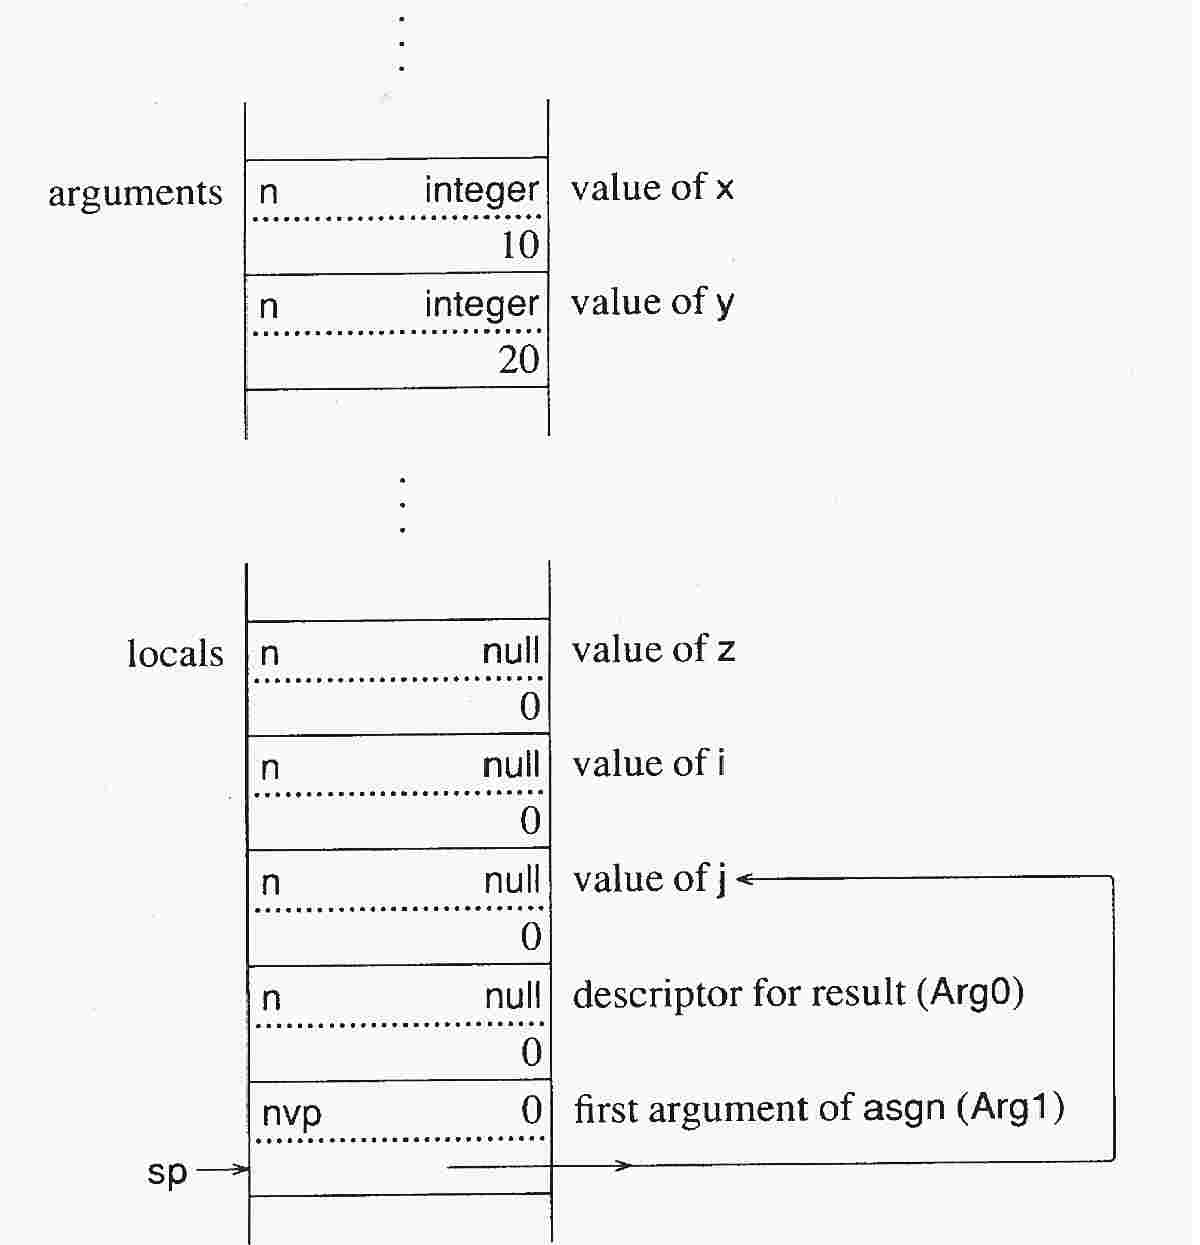
\includegraphics[width=4.0602in,height=4.1575in]{ib-img/ib-img048.jpg} 
\begin{picture}(300,310)
\put(-4,32){
\begin{picture}(300,0)
\put(-4,32){
\begin{picture}(0,0)
\put(120,0){\dvbox{null}{n}{0}}
\put(120,0){\trboxlabel{value of j}}
\put(120,32){\dvbox{null}{n}{0}}
\put(120,32){\trboxlabel{value of i}}
\put(120,64){\dvbox{null}{n}{0}}
\put(120,64){\trboxlabel{value of z}}
\put(120,64){\tlboxlabel{locals}}
\put(120,64){\upetc}
\put(120,144){\dvbox{integer}{n}{20}}
\put(120,144){\trboxlabel{value of y}}
\put(120,144){\downetc}
\put(120,176){\dvbox{integer}{n}{10}}
\put(120,176){\trboxlabel{value of x}}
\put(120,176){\tlboxlabel{arguments}}
\put(120,176){\upetc}
\end{picture}
}
\put(120,0){\dvbox{null}{n}{0}}
\put(120,0){\trboxlabel{descriptor for result (Arg0)}}
\end{picture}
}
\put(120,0){\lregptr{sp}{20}}
\put(120,0){\dvboxptr{null}{nvp}{40}{}}
\put(120,0){\downbars}
\put(120,0){\trboxlabel{first argument of asgn (Arg1)}}
\put(240,8){\line(1,0){164}}
\put(404,8){\line(0,1){80}}
\put(404,88){\vector(-1,0){120}}
\end{picture}

\ \ The Stack after \texttt{local 2}\vfill

\begin{picture}(300,380)
\put(-4,32){
\begin{picture}(0,0)
\put(-4,32){
\begin{picture}(0,0)
\put(-4,32){
\begin{picture}(0,0)
\put(120,0){\dvbox{null}{n}{0}}
\put(120,0){\trboxlabel{value of j}}
\put(120,32){\dvbox{null}{n}{0}}
\put(120,32){\trboxlabel{value of i}}
\put(120,64){\dvbox{null}{n}{0}}
\put(120,64){\trboxlabel{value of z}}
\put(120,64){\tlboxlabel{locals}}
\put(120,64){\upetc}
\put(120,144){\dvbox{integer}{n}{20}}
\put(120,144){\trboxlabel{value of y}}
\put(120,144){\downetc}
\put(120,176){\dvbox{integer}{n}{10}}
\put(120,176){\trboxlabel{value of x}}
\put(120,176){\tlboxlabel{arguments}}
\put(120,176){\upetc}
\end{picture}
}
\put(120,0){\dvbox{null}{n}{0}}
\put(120,0){\trboxlabel{descriptor for result (Arg0)}}
\end{picture}
}
\put(120,0){\dvboxptr{0}{nvp}{40}{}}
\put(120,0){\trboxlabel{first argument of asgn (Arg1)}}
\put(240,8){\line(1,0){164}}
\put(404,8){\line(0,1){80}}
\put(404,88){\vector(-1,0){120}}
\end{picture}
}
\put(120,0){\lregptr{sp}{20}}
\put(120,0){\dvbox{integer}{n}{1}}
\put(120,0){\trboxlabel{second argument of asgn (Arg2)}}
\put(120,0){\downbars}
\end{picture}

\ \ \ \ \ \ The Stack after \texttt{int 1}

\begin{picture}(300,330)(0,-30)
\put(-4,32){
\begin{picture}(300,0)
\put(120,0){\dvbox{integer}{n}{1}}
\put(120,0){\trboxlabel{value of j}}
\put(120,32){\dvbox{null}{n}{0}}
\put(120,32){\trboxlabel{value of i}}
\put(120,64){\dvbox{null}{n}{0}}
\put(120,64){\trboxlabel{value of z}}
\put(120,64){\tlboxlabel{locals}}
\put(120,64){\upetc}
\put(120,144){\dvbox{integer}{n}{20}}
\put(120,144){\trboxlabel{value of y}}
\put(120,144){\downetc}
\put(120,176){\dvbox{integer}{n}{10}}
\put(120,176){\trboxlabel{value of x}}
\put(120,176){\tlboxlabel{arguments}}
\put(120,176){\upetc}
\end{picture}
}
\put(120,0){\dvboxptr{0}{nvp}{44}}
\put(120,0){\trboxlabel{result returned by asgn}}
\put(120,0){\lregptr{sp}{20}}
\put(120,0){\downbars}
\put(240,8){\line(1,0){164}}
\put(404,8){\line(0,1){48}}
\put(404,56){\vector(-1,0){120}}
\end{picture}

\ \ \ \ The Stack after \texttt{asgn}

Note that \texttt{asgn} assigns the value of its second argument to
\texttt{j} and overwrites Arg0 with a variable descriptor, which is
left on the top of the stack.

Similarly, the virtual machine instructions for

\iconline{ \>z := x }

are

\goodbreak\iconcode{
\>pnull\\
\>local\>\>\>0\\
\>arg\>\>\>0\\
\>asgn
}

\noindent the states of the stack are


\begin{picture}(300,280)(0,-10)
\put(-4,32){
\begin{picture}(0,0)
\put(120,0){\dvbox{integer}{n}{1}}
\put(120,0){\trboxlabel{value of j}}
\put(120,32){\dvbox{null}{n}{0}}
\put(120,32){\trboxlabel{value of i}}
\put(120,64){\dvbox{null}{n}{0}}
\put(120,64){\trboxlabel{value of z}}
\put(120,64){\tlboxlabel{locals}}
\put(120,64){\upetc}
\put(120,144){\dvbox{integer}{n}{20}}
\put(120,144){\trboxlabel{value of y}}
\put(120,144){\downetc}
\put(120,176){\dvbox{integer}{n}{10}}
\put(120,176){\trboxlabel{value of x}}
\put(120,176){\tlboxlabel{arguments}}
\put(120,176){\upetc}
\end{picture}
}
\put(120,0){\dvbox{null}{n}{0}}
\put(120,0){\trboxlabel{descriptor for result (Arg0)}}
\put(120,0){\lregptr{sp}{20}}
\put(120,0){\downbars}
\end{picture}


\ \ The Stack after \texttt{pnull}


\begin{picture}(300,320)(0,-10)
\put(-4,32){
\begin{picture}(0,0)
\put(-4,32){
\begin{picture}(0,0)
\put(120,0){\dvbox{integer}{n}{1}}
\put(120,0){\trboxlabel{value of j}}
\put(120,32){\dvbox{null}{n}{0}}
\put(120,32){\trboxlabel{value of i}}
\put(120,64){\dvbox{null}{n}{0}}
\put(120,64){\trboxlabel{value of z}}
\put(120,64){\tlboxlabel{locals}}
\put(120,64){\upetc}
\put(120,144){\dvbox{integer}{n}{20}}
\put(120,144){\trboxlabel{value of y}}
\put(120,144){\downetc}
\put(120,176){\dvbox{integer}{n}{10}}
\put(120,176){\trboxlabel{value of x}}
\put(120,176){\tlboxlabel{arguments}}
\put(120,176){\upetc}
\end{picture}
}
\put(120,0){\dvbox{null}{n}{0}}
\put(120,0){\trboxlabel{descriptor for result (Arg0)}}
\end{picture}
}
\put(120,0){\dvboxptr{0}{nvp}{44}{}}
\put(120,0){\lregptr{sp}{20}}
\put(120,0){\trboxlabel{first argument of asgn (Arg1)}}
\put(244,8){\line(1,0){160}}
\put(404,8){\line(0,1){144}}
\put(404,152){\vector(-1,0){116}}
\put(120,0){\downbars}
\end{picture}

\ \ The Stack after \texttt{local 0}


\begin{picture}(300,300)(0,5)
\put(-4,32){
\begin{picture}(0,0)
\put(-4,32){
\begin{picture}(0,0)
\put(-4,32){
\begin{picture}(0,0)
\put(120,0){\dvbox{integer}{n}{1}}
\put(120,0){\trboxlabel{value of j}}
\put(120,32){\dvbox{null}{n}{0}}
\put(120,32){\trboxlabel{value of i}}
\put(120,64){\dvbox{null}{n}{0}}
\put(120,64){\trboxlabel{value of z}}
\put(120,64){\tlboxlabel{locals}}
\put(120,64){\upetc}
\put(120,144){\dvbox{integer}{n}{20}}
\put(120,144){\trboxlabel{value of y}}
\put(120,144){\downetc}
\put(120,176){\dvbox{integer}{n}{10}}
\put(120,176){\trboxlabel{value of x}}
\put(120,176){\tlboxlabel{arguments}}
\put(120,176){\upetc}
\end{picture}
}
\put(120,0){\dvbox{null}{n}{0}}
\put(120,0){\trboxlabel{descriptor for result (Arg0)}}
\put(120,0){\downbars}
\end{picture}
}
\put(120,0){\dvboxptr{0}{nvp}{44}{}}
\put(120,0){\trboxlabel{first argument of asgn (Arg1)}}
\put(244,8){\line(1,0){160}}
\put(404,8){\line(0,1){144}}
\put(404,152){\vector(-1,0){116}}
\end{picture}
}
\put(120,0){\dvboxptr{0}{nvp}{44}{}}
\put(120,0){\lregptr{sp}{20}}
\put(120,0){\trboxlabel{second argument of asgn (Arg2)}}
\put(120,0){\downbars}
\put(244,8){\line(1,0){180}}
\put(424,8){\line(0,1){288}}
\put(424,296){\vector(-1,0){136}}
\end{picture}

\ \ \ \ The Stack after \texttt{arg 0}

\begin{picture}(300,260)(0,5)
\put(-4,32){
\begin{picture}(0,0)
\put(120,0){\dvbox{integer}{n}{1}}
\put(120,0){\trboxlabel{value of j}}
\put(120,32){\dvbox{null}{n}{0}}
\put(120,32){\trboxlabel{value of i}}
\put(120,64){\dvbox{integer}{n}{10}}
\put(120,64){\trboxlabel{value of z}}
\put(120,64){\tlboxlabel{locals}}
\put(120,64){\upetc}
\put(120,144){\dvbox{integer}{n}{20}}
\put(120,144){\trboxlabel{value of y}}
\put(120,144){\downetc}
\put(120,176){\dvbox{integer}{n}{10}}
\put(120,176){\trboxlabel{value of x}}
\put(120,176){\tlboxlabel{arguments}}
\put(120,176){\upetc}
\end{picture}
}
\put(120,0){\dvboxptr{0}{nvp}{44}{}}
\put(120,0){\trboxlabel{result returned by asgn}}
\put(120,0){\lregptr{sp}{20}}
\put(120,0){\downbars}
\put(244,8){\line(1,0){160}}
\put(404,8){\line(0,1){112}}
\put(404,120){\vector(-1,0){116}}
\end{picture}

\ \ \ \ The Stack after \texttt{asgn}


\subsection[8.2.3 Operators]{8.2.3 \textbf{Operators}}

There is a virtual machine instruction for each of the forty-two
operators in Icon. The instructions random and asgn described
previously are examples. Casting Icon operators as virtual machine
instructions masks a considerable amount of complexity, since few Icon
operators are simple. For example, although x + y appears to be a
straightforward computation, it involves checking the types of x and
y, converting them to numeric types if they are not already numeric,
and terminating with an error message if this is not possible. If x
and y are numeric or convertible to numeric, addition is
performed. Even this is not simple, since the addition may be integer
or floating-point, depending on the types of the arguments. For
example, if x is an integer and y is a real number, the integer is
converted to a real number. None of these computations is evident in
the virtual machine instructions produced for this expression, which
are

\goodbreak
\iconcode{
\>pnull\\
\>local\>\>\> x\\
\>local\>\>\> y\\
\>plus
}

In the instructions given previously, the indices that are used to
access identifiers have been replaced by the names of the identifiers,
which are assumed to be local. This convention is followed in
subsequent virtual machine instructions for ease of reading.

Augmented assignment operations do not have separate virtual machine
instructions. Instead, the instruction \texttt{dup} first pushes a
null descriptor and then pushes a duplicate of the descriptor that was
previously on top of the stack.  For example, the virtual machine
instructions for

\iconline{ \>i +:= 1 }

are

\goodbreak
\iconcode{
\>pnull\\
\>local\>\>\> i\\
\>dup\\
\>int\>\>\> 1\\
\>plus\\
\>asgn
}

The stack after the execution of \texttt{local} is

\begin{picture}(300,120)(0,-20)
\put(120,0){\dvboxptr{0}{nvp}{40}{local i}}
\put(120,0){\lregptr{sp}{20}}
\put(120,0){\downbars}
\put(120,32){\dvbox{null}{n}{0}}
\put(120,32){\upetc}
\end{picture}

The execution of \texttt{dup} produces

\begin{picture}(300,180)(0,-20)
\put(-4,74){
\begin{picture}(0,0)(0,10)
\put(120,0){\dvboxptr{0}{nvp}{40}{local i}}
\put(120,32){\dvbox{null}{n}{0}}
\put(120,32){\upetc}
\end{picture}
}
\put(120,32){\dvbox{null}{n}{0}}
\put(120,0){\dvbox{0}{nvp}{}}
\put(120,0){\ruptr{30}{64}}
\put(120,0){\lregptr{sp}{20}}
\put(120,0){\downbars}
\end{picture}

The \texttt{dup} instruction simply takes the place of the
\texttt{pnull} and second \texttt{local} instructions in the virtual
machine instructions for

\iconline{ \>i := i + 1 }

which are

\goodbreak
\iconcode{
\>pnull\\
\>local\>\>\>i\\
\>pnull\\
\>local\>\>\>i\\
\>int\>\>\>1\\
\>plus\\
\>asgn
}

In this case, only a single \texttt{local} instruction is avoided. If
the variable to which the assignment is made is not just an identifier
but, instead, a more complicated construction, as in

\iconline{ \>a[j] +:= 1 }

\noindent substantial computation may be saved by duplicating the
result of the first argument expression instead of recomputing it.

\subsection[8.2.4 Functions]{8.2.4 Functions}

While the meaning of an operation is fixed and can be translated into
a specific virtual machine instruction, the meaning of a function call
can change during program execution. The value of the function also
can be computed. as in

\iconline{ \>(p[i])(x, y) }

The general form of a call is

\iconline{
\>\textit{expr0(expr1, expr2, } ..., \textit{exprn)}
}
The corresponding virtual machine instructions are

\goodbreak
\iconcode{
\>code for expr0\\
\>code for expr1\\
\>code for expr2\\
\>\>...\\
\>code for exprn\\
\>invoke n
}

The \texttt{invoke} instruction is relatively complicated, since the
value of \textit{expr0 }may be a procedure, an integer (for mutual
evaluation), or even a value that is erroneous. Function invocation is
discussed in detail in Chapter 10.

\subsection[8.2.5 Self-Modifying Instructions]{8.2.5 Self-Modifying Instructions}

Seven opcodes, including several described in the preceding
sections, contain operands whose values are addresses within the
virtual machine icode. The linker cannot know these run-time
addresses, so instead, it generates the instructions with byte
offsets, relative to the current instruction.  At runtime the
interpreter obtains the address in question by adding the current
instruction pointer to the offset.  In order to avoid repeating this
calculation every time the instruction executes, the interpreter
stores the pointer in place of the offset and modifies the opcode to
indicate that the offset has been converted to a pointer.  The self
modifying instructions and their address-holding counterparts are:

\iconcode{
\>   str    \>\>\>\> Astr \\
\>   cset   \>\>\>\> Astr\\
\>   real   \>\>\>\> Areal\\
\>   global \>\>\>\> Aglobal \\
\>   static \>\>\>\> Astatic\\
\>   goto   \>\>\>\> Agoto\\
\>   mark   \>\>\>\> Amark
}

The details of the \texttt{str} instruction illustrate the code for
self-modifying instructions. There are several points of interest. The
opcode must be modified from \texttt{Op\_Str} to \texttt{Op\_Astr} and
its offset operand modified to contain a pointer.  Depending on
whether Concurrent is enabled, the self-modification of the
instruction is done by either two "Put" macros
(\texttt{PutOp(Op\_Astr)} on the current opcode and
\texttt{PutWord(opnd)}), or by a \texttt{PutInstr(Op\_Astr, opnd, 2)}
after the instruction pointer is referring to the operand.  This is
because these self-modifying instructions create a race condition when
executed concurrently and thus require mutex locks.  After
(potentially) waiting to obtain a lock, the instruction must check
again to see if a competing thread has already modified its opcode,
and if so, it jumps down to the code for \texttt{Op\_Astr}.


\iconcode{
\>\>\>	 case Op\_Str:		/* string */ \\
\#ifdef Concurrent \\
\>\>\>\>    MUTEX\_LOCKID(MTX\_OP\_ASTR); \\
\>\>\>\>    if (ipc.op[-1] == Op\_Astr) \{ \\
\>\>\>\>\>     MUTEX\_UNLOCKID(MTX\_OP\_ASTR); goto L\_astr; \} \\
\#else					/*Concurrent*/ \\
\>\>\>\>    PutOp(Op\_Astr); \\
\#endif					/*Concurrent*/ \\
\>\>\>\>    PushVal(GetWord) \\
\ \\
\>\>\>\>	... \\
\>\>\>\>       opnd = (word)strcons + GetWord; \\
\ \\
\#ifdef Concurrent \\
\>\>\>\>    PutInstr(Op\_Astr, opnd, 2); \\
\#else					/*Concurrent*/ \\
\>\>\>\>    PutWord(opnd); \\
\#endif					/*Concurrent*/ \\
\>\>\>\>    PushAVal(opnd); \\
\>\>\>\>    InterpEVValD((dptr)(rsp-1), e\_literal); \\
\ \\
\>\>\>\>    MUTEX\_UNLOCKID(MTX\_OP\_ASTR); \\
\>\>\>\>    break; \\
\ \\
\>\>\>	 case Op\_Astr:		/* string, absolute address */ \\
L\_astr: \\
\>\>\>\>    PushVal(GetWord); \\
\>\>\>\>    PushAVal(GetWord); \\
\>\>\>\>    InterpEVValD((dptr)(rsp-1), e\_literal); \\
\>\>\>\>    break;
}


\section[8.3 The Interpreter Proper]{8.3 The Interpreter Proper}
\subsection[8.3.1 The Interpreter Loop]{8.3.1 The Interpreter Loop}

The interpreter, which is called \texttt{interp()}, is basically
simple in structure. It maintains a location in the icode
(\texttt{ipc}) and begins by fetching the instruction pointed to by
\texttt{ipc} and incrementing \texttt{ipc} to the next location. It
then branches to a section of code for processing the virtual machine
instruction that it fetched. The interpreter loop is

\goodbreak
\iconcode{
\>for (;;) \{\\
\>\>op = GetWord;\\
\>\>switch (op) \{\\
\>\>\>...\\
\>\>\>case Op\_Asgn:\\
\>\>\>...\\
\>\>\>case Op\_Plus:\\
\>\>\>...\\
\>\>\>\}\\
\>\>continue;\\
\>\>\>...\\
\>\>\}
}

\noindent
where \texttt{GetWord} is a macro that is defined to be \texttt{(*ipc++)}.

Macros are used extensively in the interpreter to avoid repetitious
coding and to make the interpreter easier to read.  The coding is
illustrated by the case clause for the instruction \texttt{plus}:

\goodbreak
\iconcode{
\>case Op\_Plus:\ \ /* e1 + e2 */\\
\>\>Setup\_Op(2);\\
\>\>DerefArg(1);\\
\>\>DerefArg(2);\\
\>\>Call\_Op;\\
\>\>break;
}



\texttt{Setup\_Op(n)} sets up a pointer to the address of Arg0 on the
interpreter stack. The resulting code is

\iconline{\>rargp = (dptr)(sp - 1) - n;}

The value of \texttt{n} is the number of arguments on the stack.

\texttt{DerefArg(n)} dereferences argument \texttt{n}. If it is a
variable, it is replaced by its value. Thus, dereferencing is done in
place by changing descriptors on the interpreter stack.

\texttt{Call\_Cond} calls the appropriate C function with a pointer to
the interpreter stack as provided by \texttt{Setup\_Op(n)}. The
function itself is obtained by looking up \texttt{op} in an array of
pointers to functions.  The code produced by \texttt{Call\_Cond} is
(almost)

\goodbreak
\iconcode{
\>(*(optab(op]) )(rargp);\\
\>sp = (word * )rargp + 1:
}

In the case where a C function produces a result, as plus always does,
that result is placed in the Arg0 descriptor on the interpreter stack,
as illustrated by the examples in Chapters 4 and 5. The interpreter
adjusts sp to point to the v-word of Arg0. The break transfers control
to the end of the switch statement, where a continue statement
transfers control to the beginning of the interpreter loop, and the
next instruction is fetched.

As illustrated earlier, some virtual machine instructions have
operands, which follow the instructions in the icode. The interpreter
code for such an instruction fetches its operands. An example is

\iconline{ \>int n }

The interpreter code for int is

\goodbreak
\iconcode{
\>case Op\_Int: /* integer */\\
\>PushVal(D\_Integer);\\
\>PushVal(GetWord);\\
\>break;
}

\texttt{PushVal(x)} pushes x onto the interpreter stack. Thus, the descriptor
for the integer is constructed by first pushing the constant \texttt{D\_Integer}
for the d-word and then pushing the fetched operand for the v-word.

\subsection[8.3.2 Interpreter State Variables]{8.3.2 Interpreter State Variables}

The state of the interpreter is characterized by several variables,
called \textit{i-state variables}. Two i-state variables mentioned
previously are sp, the interpreter stack pointer, and ipc, the
interpreter ``program counter.''

The interpreter also pushes frames on the interpreter stack when
procedures are called. Such frames are analogous to the frames pushed
on the C stack when a C function is called, and contain information
(typically i-state variables) that is saved when a procedure is called
and restored when a procedure returns. There are other kinds of frames
for special aspects of expression evaluation; these are described in
Chapter 9. Pointers to frames are themselves i-state variables.

The proper maintenance of i-state variables is a central aspect of the
interpreter and is discussed in detail in the next two chapters.

Retrospective: The interpreter models, in software, the hardware of a
cpu. The instruction fetch, the execution of operations, and the flow
of control are basically the same as that in hardware execution, as is
the use of a stack.

An interpreter offers great flexibility. It is easy to add virtual
machine instructions, change existing ones, or change how they are
implemented. Tracking and monitoring also are easy to add. The
interpreter is machine-independent and portable. These advantages
outweigh the loss in efficiency associated with emulating hardware in
software.

\bigskip

\noindent\textbf{EXERCISES}

\liststyleLvi
\begin{enumerate}
\item Why is it advantageous for the first argument of str to be the
length of the string, rather than its address?

\item Show the states of the stack for the execution of the virtual
machine instructions for the following Icon expressions:

\iconcode{
\>   i := i + 1 \\
\>   l := ???j
}

\item Give an example for which

\iconline{
\> expr1 := expr1 + expr2
}

produces a different result from

\iconline{
\> expr1 +:= expr2
}

\item Describe, in general terms, what would be involved in adding a
new operator to Icon.

\item Describe, in general terms, what would be involved in adding a
new kind of literal to Icon.

\item Suppose that functions were bound at translation time instead of
being source-language values. How might the virtual machine be
modified to take advantage of such a feature?  What effect would this
have on the interpreter?

\end{enumerate}

\chapter{Expression Evaluation}

\textsc{Perspective}: The preceding chapter presents the essentials of
the interpreter and expression evaluation as it might take place in a
conventional programming language in which every expression produces
exactly one result. For example, expressions such as

{\ttfamily\mdseries
\ \ \ i := j}

{\ttfamily\mdseries
\ \ \ k := i + j}

{\ttfamily\mdseries
\ \ \ i +:= ?k}

\noindent each produce a single result: they can neither fail nor can
they produce sequences of results.

The one feature of Icon that distinguishes it most clearly from other
programming languages is the capacity of its expression-evaluation
mechanism to produce no result at all or to produce more than one
result. From this capability come unconventional methods of
controlling program flow, novel control structures, and goal-directed
evaluation.

The generality of this expression-evaluation mechanism alone sets Icon
apart from other programming languages. While generators, in one form
or another, exist in a number of programming languages, such as IPL-V
(Newell 1961), CLU (Liskov 1981), Alphard (Shaw 1981), and SETL
(Dewar, Schonberg, and Schwartz 1981), such generators are limited to
specific constructs, designated contexts, or restricted types of
data. Languages with pattern-matching facilities, such as SNOBOL4
(Griswold, Poage, and Polonsky 1971), InterLisp (Teitelman 1974), and
Prolog (Clocksin and Mellish 1981), generate alternative matches, but
only within pattern matching.

Just as Icon's expression-evaluation mechanism distinguishes it from
other programming languages, it is also one of the most interesting
and challenging aspects of Icon's implementation. Its applicability in
every context and to all kinds of data has a pervasive effect on the
implementation.


\section[9.1 Bounded Expressions]{9.1 Bounded Expressions}

A clear understanding of the semantics of expression evaluation in
Icon is necessary to understand the implementation.  One of the most
important concepts of expression evaluation in Icon is that of a
\textit{bounded expression, }within which backtracking can take
place. However, once a bounded expression has produced a result, it
cannot be resumed for another result. For example, in

{\ttfamily\mdseries
\ \ \ write(i = find(s1,s2))}

\noindent find may produce a result and may be resumed to produce
another result if the comparison fails. On the other hand, in

{\ttfamily\mdseries
\ \ \ write(i = find(s1, s2))}

{\ttfamily\mdseries
\ \ \ write(j = find(s1, s3))}

\noindent the two lines constitute separate expressions. Once the
evaluation of the expression on the first line is complete, it cannot
be resumed. Likewise, the evaluation of the expression on the second
line is not affected by whether the expression on the first line
succeeds or fails. However, if the two lines are joined by a
conjunction operation, as in

{\ttfamily\mdseries
\ \ \ write(i = find(s1, s2)) \&}

{\ttfamily\mdseries
\ \ \ write(i = find(s1, s3))}

\noindent they are combined into a larger single expression and the
expression on the second line is not evaluated if the expression on
the first line fails. Similarly, if the expression on the first line
succeeds, but the expression on the second line fails, the expression
on the first line is resumed.

The reason for the difference in the two cases is obscured by the fact
that the Icon translator automatically inserts a semicolon at the end
of a line on which an expression is complete and for which a new
expression begins on the next line.

Consequently, the first example is equivalent to

{\ttfamily\mdseries
\ \ \ write(i = find(s1, s2));}

{\ttfamily\mdseries
\ \ \ write(i = find(s1 , s3))}

The difference between the semicolon and the conjunction operator is
substantial. A semicolon bounds an expression, while an operator binds
its operands into a single expression.

Bounded expressions are enclosed in ovals in the following examples to
make the extent of backtracking clear. A compound expression, for
example, has the following bounded expressions:

\begin{center}
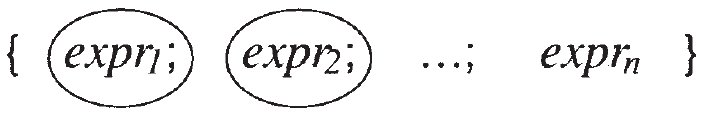
\includegraphics[width=3.2819in,height=0.4736in]{ib-img/ib-img057.jpg}
\end{center}

Note that \textit{exprn }is not, of itself, a bounded expression.
However, it may be part of a larger bounded expression, as in

\begin{center}
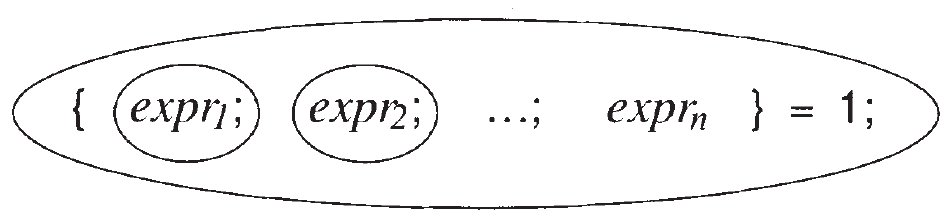
\includegraphics[width=3.5425in,height=0.8173in]{ib-img/ib-img058.jpg}
\end{center}

Here \textit{exprn} is part of the bounded expression for the
comparison operator. The entire enclosing bounded expression is a
consequence of the final semicolon. In the absence of the context
provided by this semicolon, the entire expression might be part of a
larger enclosing bounded expression, and so on.

The separation of a procedure body into a number of bounded
expressions, separated by semicolons (explicit or implicit) and other
syntactic constructions, is very important. Otherwise, a procedure
body would consist of a single expression, and failure of any
component would propagate throughout the entire procedure
body. Instead, control backtracking is limited in scope to abounded
expression, as is the lifetime (and hence stack space) for temporary
computations.

Bounded expressions are particularly important in control
structures. For example, in the if-then-else control structure, the
control expression is bounded but the other expressions are not:

\begin{center}
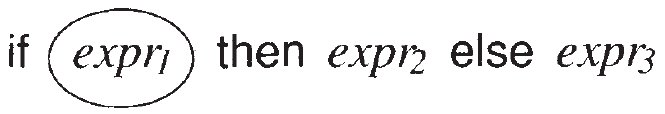
\includegraphics[width=3.5508in,height=0.5244in]{ib-img/ib-img059.jpg}
\end{center}

As with the compound expression illustrated earlier, \textit{expr2} or
\textit{exp13} (whichever is selected) may be the part of a larger
bounded expression. An example is

\begin{center}

\includegraphics[width=4.0839in,height=0.4571in]{ib-img/ib-img060.jpg}
\end{center}

If the control expression were not a separate bounded expression, the
failure of \textit{expr2} or \textit{exp13} would result in
backtracking into it and the if-then-else expression would be
equivalent to

{\ttfamily\mdseries
\textit{\ \ \ (expr1 }\& \textit{expr2) }{\textbar} \textit{expr3}}

\noindent which is hardly what is meant by if-then-else.

In a while-do loop, the control expression and the expression in the
do clause are both bounded:

\begin{center}
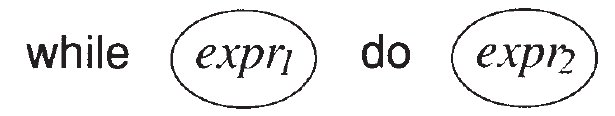
\includegraphics[width=2.8339in,height=0.4992in]{ib-img/ib-img061.jpg}
\end{center}

The two bounded expressions ensure that the expressions are evaluated
independently of each other and any surrounding context. For example,
if \textit{expr2} fails, there is no control backtracking into
\textit{expr}.

\subsection[9.1.1 Expression Frames]{9.1.1 Expression Frames}

In the implementation of Icon, the scope of backtracking is delineated
by \textit{expression frames}. The virtual machine instruction

{\ttfamily\mdseries
\ \ \ mark L1}

\noindent starts an expression frame. If the subsequent expression
fails, \texttt{ipc} is set to the location in the icode that
corresponds to \texttt{L1}. The value of \texttt{ipc} for a label is
relative to the location of the icode that is read in from the icode
file. For simplicity in the description that follows, the value of
\texttt{ipc} is referred to just by the name of the corresponding
label.

The \texttt{mark} instruction pushes an \textit{expression frame
marker }onto the stack and sets the expression frame pointer,
\texttt{efp}, to it. Thus, \texttt{efp} indicates the beginning of the
current expression frame. There is also a generator frame pointer,
\texttt{gfp}, which points to another kind of frame that is used to
retain information when an expression suspends with a result and is
capable of being resumed for another. Generator frames are described
in Sec. 9.3. The mark instruction sets \texttt{gfp} to zero,
indicating that there is no suspended generator in a new expression
frame.

An expression frame marker consists of four words: the value
\texttt{ipc} for the argument of mark (called the failure
\texttt{ipc}), the previous \texttt{efp}, the previous \texttt{gfp},
and \texttt{ilevel}, which is related to suspended generators:


\ \  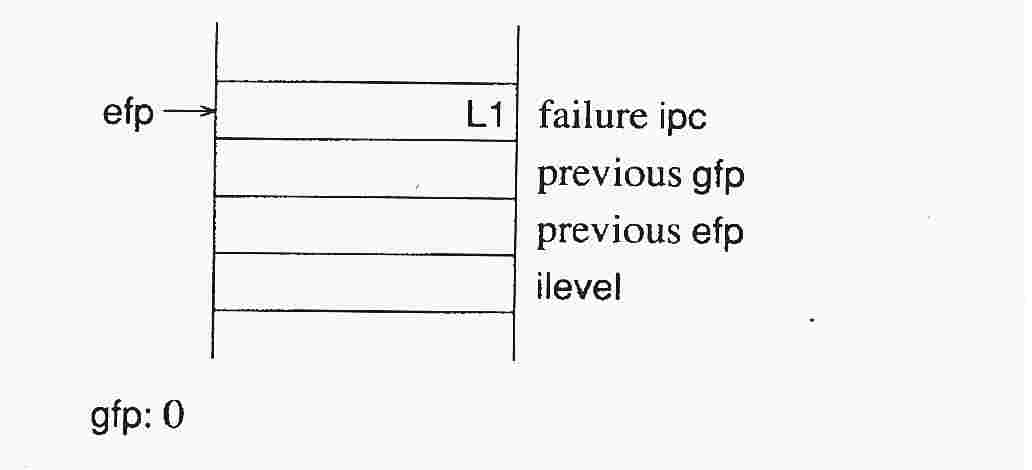
\includegraphics[width=3.5272in,height=1.5689in]{ib-img/ib-img062.jpg} 


An expression frame marker is declared as a C structure:

{\ttfamily\mdseries
\ \ \ struct ef\_marker \{\ \ \ \ /* expression frame marker */}

{\ttfamily\mdseries
\ \ \ \ \ \ word *ef\_failure;\ \ \ \ /*\ \ failure ipc */}

{\ttfamily\mdseries
\ \ \ \ \ \ struct ef\_marker *ef\_efp;\ \ /*\ \ efp */}

{\ttfamily\mdseries
\ \ \ \ \ \ struct gf\_marker *ef\_gfp;\ \ /*\ \ gfp */}

{\ttfamily\mdseries
\ \ \ \ \ \ word ef\_ilevel;\ \ \ \ \ \ /*\ \ ilevel */}


This structure is overlaid on the interpreter stack in order to
reference its components. The code for the \texttt{mark} instruction
is

{\ttfamily\mdseries
\ \ \ case Op\_Mark:\textit{\ \ /* }create expression frame marker \textit{*/}}

{\ttfamily\mdseries
\ \ \ \ \ \ newefp = (struct ef\_marker *)(sp + 1);}

{\ttfamily\mdseries
\ \ \ \ \ \ opnd = GetWord;}

{\ttfamily\mdseries
\ \ \ \ \ \ opnd += (word)ipc;}

{\ttfamily\mdseries
\ \ \ \ \ \ newefp-{\textgreater}ef\_failure = (word *)opnd;}

{\ttfamily\mdseries
\ \ \ \ \ \ newefp-{\textgreater}ef\_gfp = gfp;}

{\ttfamily\mdseries
\ \ \ \ \ \ newefp-{\textgreater}ef\_efp = efp;}

{\ttfamily\mdseries
\ \ \ \ \ \ newefp-{\textgreater}ef\_ilevel = ilevel;}

{\ttfamily\mdseries
\ \ \ \ \ \ sp += Wsizeof(*efp);}

{\ttfamily\mdseries
\ \ \ \ \ \ efp = newefp;}

{\ttfamily\mdseries
\ \ \ \ \ \ gfp = 0;}

{\ttfamily\mdseries
\ \ \ \ \ \ break;}

The macro \texttt{Wsizeof(x)} produces the size of \texttt{x} in words.

An expression frame is removed by the virtual machine instruction

{\ttfamily\mdseries
\ \ \ unmark}

\noindent which restores the previous \texttt{efp} and \texttt{gfp}
from the current expression frame marker and removes the current
expression frame by setting \texttt{sp} to the word just above the
frame marker.

The use of \texttt{mark} and \texttt{unmark} is illustrated by

{\ttfamily\mdseries
\ \ \ if expr1 then \textit{expr2 }else \textit{expr3}}

\noindent for which the virtual machine instructions are

{\ttfamily\mdseries
\ \ \ \ \ \ mark L1}

{\ttfamily\mdseries
\ \ \ \ \ \ code for expr1}

{\ttfamily\mdseries
\ \ \ \ \ \ unmark}

{\ttfamily\mdseries
\ \ \ \ \ \ code for expr2}

{\ttfamily\mdseries
\ \ \ \ \ \ goto L2}

{\ttfamily\mdseries
L1:}

{\ttfamily\mdseries
\ \ \ \ \ \ code for expr3}

{\ttfamily\mdseries
L2:}

The \texttt{mark} instruction creates an expression frame for the
evaluation of \textit{expr1}. If \textit{expr1} produces a result, the
\texttt{unmark} instruction is evaluated, removing the expression
frame for \textit{expr1}, along with the result produced by
\textit{expr1}. Evaluation then proceeds in \textit{expr2}.

If \textit{expr1} fails, control is transferred to the location in the
icode corresponding to \texttt{L1} and the \texttt{unmark} instruction
is not executed. In the absence of generators, failure also removes
the current expression frame, as described in Sec. 9.2.


It is necessary to save the previous value of \texttt{efp} in a new
expression marker, since expression frames may be nested. This occurs
in interesting ways in some generative control structures, which are
discussed in Sec. 9.4. Nested expression frames also occur as a result
of evaluating compound expressions, such as

{\ttfamily\mdseries
\ \ \ while expr1 do ifexpr2thenexpr2}


\section[9.2 Failure]{9.2 Failure}

The interesting aspects of implementing expression evaluation in Icon
can be divided into two cases: without generators and with
generators. The possibility of failure in the absence of generators is
itself of interest, since it occurs in other programming languages,
such as SNOBOL4. This section describes the handling of failure and
assumes, for the moment, that there are no generators. The next
section describes generators.

In the absence of generators, if failure occurs anywhere in an
expression, the entire expression fails without any further
evaluation. For example, in the expressions

{\ttfamily\mdseries
\ \ \ i := numeric(s)}

{\ttfamily\mdseries
\ \ \ line := read(f)}

\noindent if \texttt{numeric(s)} fails in the first line, the
assignment is not performed and evaluation continues immediately with
the second line. In the implementation, this amounts to removing the
current expression frame in which failure occurs and continuing with
\texttt{ipc} set to the failure \texttt{ipc} from its expression frame
marker.

The virtual machine instructions for the previous example are

{\ttfamily\mdseries
\ \ \ mark L1}

{\ttfamily\mdseries
\ \ \ pnull}

{\ttfamily\mdseries
\ \ \ local i}

{\ttfamily\mdseries
\ \ \ global numeric}

{\ttfamily\mdseries
\ \ \ local s}

{\ttfamily\mdseries
\ \ \ invoke 1}

{\ttfamily\mdseries
\ \ \ asgn}

{\ttfamily\mdseries
\ \ \ unmark}

{\ttfamily\mdseries
L1:}

{\ttfamily\mdseries
\ \ \ mark L2}

{\ttfamily\mdseries
\ \ \ pnull}

{\ttfamily\mdseries
\ \ \ local line}

{\ttfamily\mdseries
\ \ \ global read}

{\ttfamily\mdseries
\ \ \ local f}

{\ttfamily\mdseries
\ \ \ invoke 1}

{\ttfamily\mdseries
\ \ \ asgn}

{\ttfamily\mdseries
\ \ \ unmark}

{\ttfamily\mdseries
L2:}

Prior to the evaluation of the expression on the first line, there is
some expression frame on the stack:

\ \  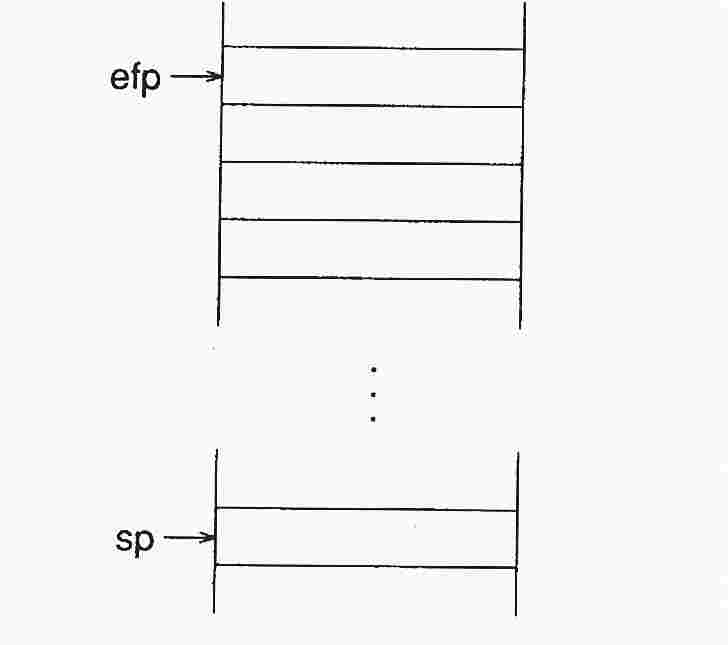
\includegraphics[width=2.4575in,height=2.1543in]{ib-img/ib-img063.jpg} 

The instruction

{\ttfamily\mdseries
\ \ \ mark L1}

\noindent starts a new expression frame. The execution of subsequent
virtual machine instructions pushes additional descriptors.  The state
of the stack when numeric is called by the \texttt{invoke} instruction is

\ \  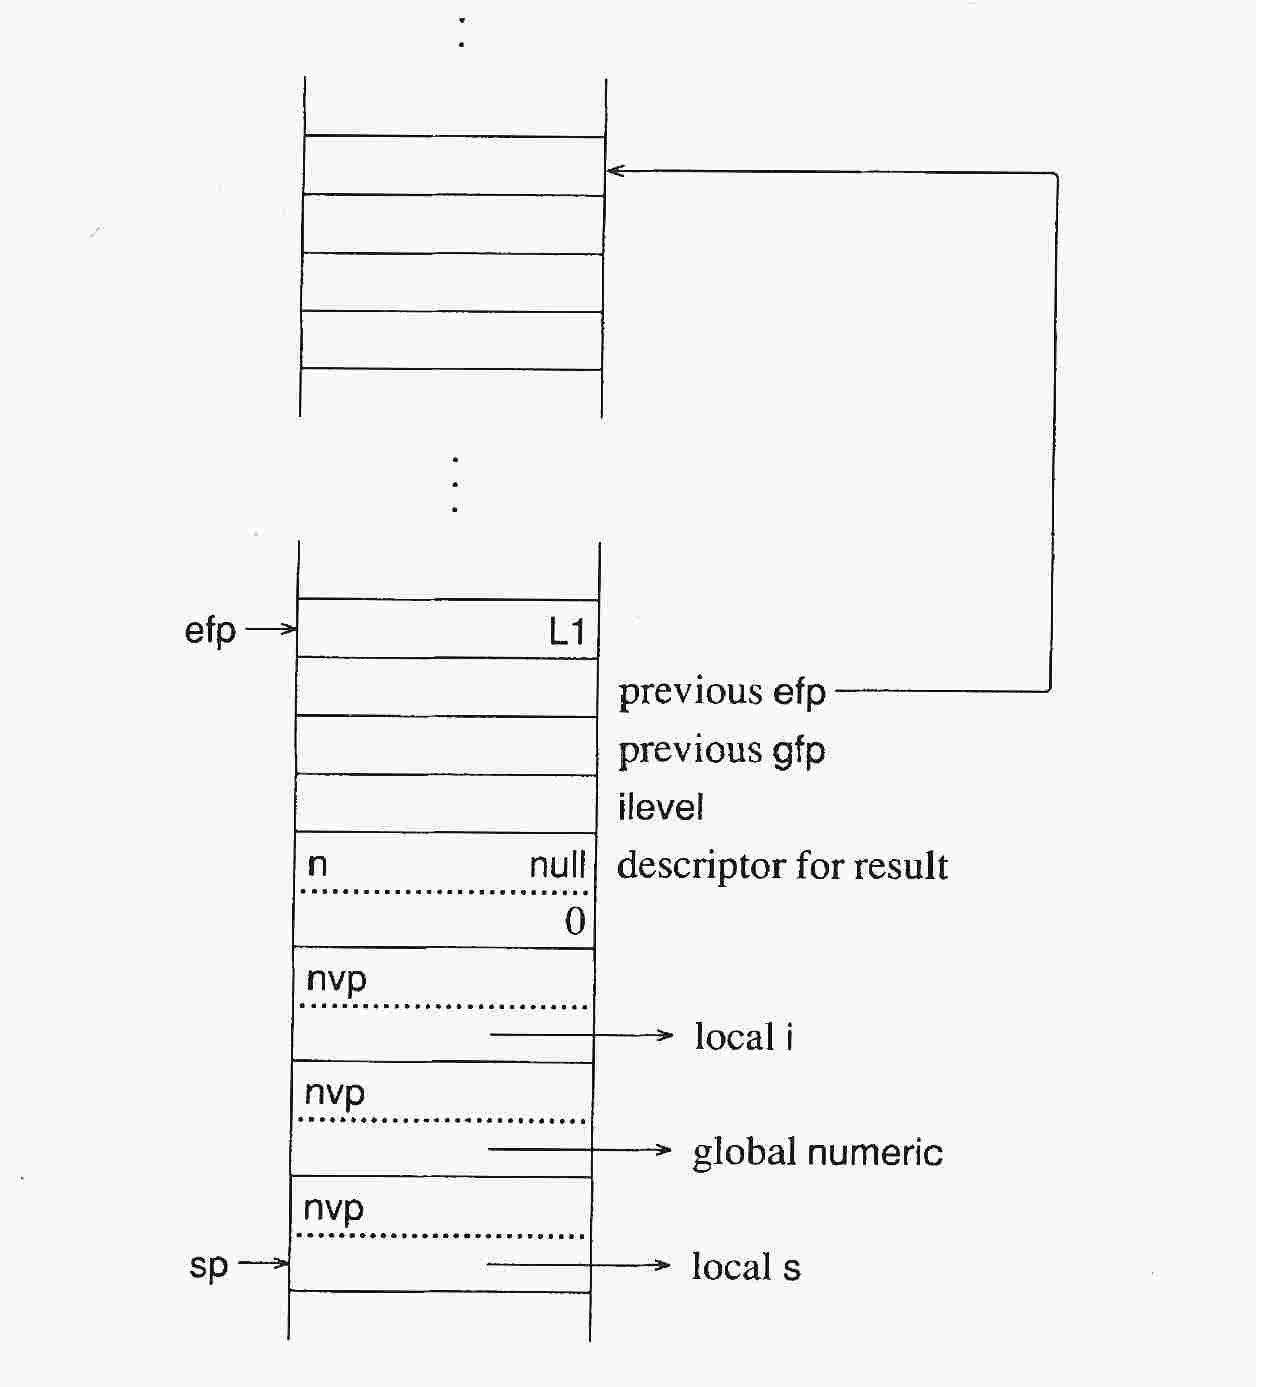
\includegraphics[width=4.2752in,height=4.6319in]{ib-img/ib-img064.jpg} 

If \texttt{numeric(s)} fails, \texttt{efp} and \texttt{sp} are reset,
so that the stack is in the same state as it was prior to the
evaluation of the expression on the first line:

\ \  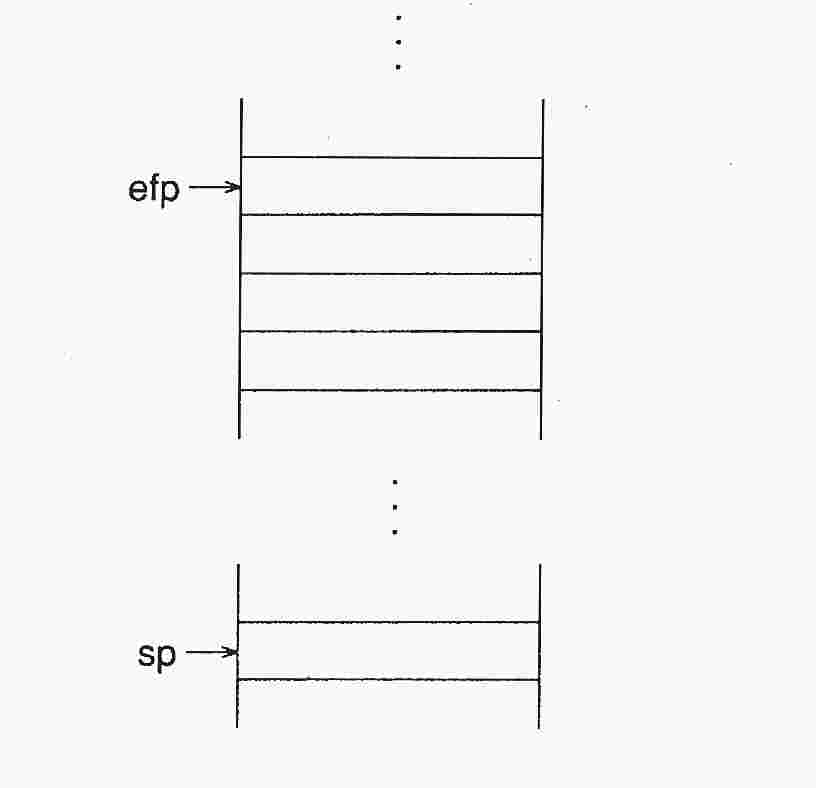
\includegraphics[width=2.778in,height=2.6311in]{ib-img/ib-img065.jpg} 

Control is transferred to the location in the icode corresponding to
\texttt{L1}, and the execution of

{\ttfamily\mdseries
\ \ \ mark L2}

\noindent starts a new expression frame by pushing a new expression
frame marker onto the stack.

It is worth noting that failure causes only the current expression
frame to be removed and changes \texttt{ipc} to the failure
\texttt{ipc}. Any remaining virtual machine instructions in the
current expression frame are bypassed; failure is simple and quick.

Failure can occur at three levels: directly from the virtual machine
instruction \texttt{efail}, from a C function that implements an
operator or function (as in the previous example), or from an Icon
procedure.


When a conditional operator or function returns, it signals the
interpreter, indicating whether it is producing a result or failing by
using one of the RTL forms of return, \texttt{return} or
\texttt{fail}. These RTL constructs simply produce return statements
with different returned values.

The code in the interpreter for a conditional operation is illustrated by

{\ttfamily\mdseries
\ \ \ case Op\_Numlt:\ \ /* e1 {\textless} e2 */}

{\ttfamily\mdseries
\ \ \ \ \ \ Setup\_Op(2);}

{\ttfamily\mdseries
\ \ \ \ \ \ DerefArg(1);}

{\ttfamily\mdseries
\ \ \ \ \ \ DerefArg(2) ;}

{\ttfamily\mdseries
\ \ \ \ \ \ Call\_Cond;}


The macro \texttt{Call\_Cond} is similar to \texttt{Call\_Op}
described in Sec. 8.3.1, but it tests the signal returned by the C
function. If the signal corresponds to the production of a result, the
break is executed and control is transferred to the beginning of the
interpreter loop to fetch the next virtual machine instruction. On the
other hand, if the signal corresponds to failure, control is
transferred to the place in the interpreter that handles failure,
\texttt{efail}.


An Icon procedure can fail in three ways: by evaluating the expression
fail, by the failure of the argument of a return expression, or by
flowing off the end of the procedure body. The virtual machine
instructions generated for the three cases are similar. For example,
the virtual machine instructions for

{\ttfamily\mdseries
\ \ \ if i {\textless} j then fail else write(j)}


are

{\ttfamily\mdseries
\ \ \ mark L1}

{\ttfamily\mdseries
\ \ \ pnull}

{\ttfamily\mdseries
\ \ \ local i}

{\ttfamily\mdseries
\ \ \ local j}

{\ttfamily\mdseries
\ \ \ numlt}

{\ttfamily\mdseries
\ \ \ unmark}

{\ttfamily\mdseries
\ \ \ pfail}

{\ttfamily\mdseries
L1:}

{\ttfamily\mdseries
\ \ \ global write}

{\ttfamily\mdseries
\ \ \ local j}

{\ttfamily\mdseries
\ \ \ invoke 1}

The virtual machine instruction \texttt{pfail} first returns from the
current procedure call (see Sec. 10.3), and then transfers to
\texttt{efail}.


\section[9.3 Generators and Goal{}-Directed Evaluation]{9.3 Generators and Goal-Directed Evaluation}

The capability of an expression not to produce a result is useful for
controlling program flow and for bypassing unneeded computation, but
generators add the real power and expressiveness to the
expression-evaluation semantics of Icon. It should be no surprise that
generators also present difficult implementation problems. There are
several kinds of generators, including those for control structures,
functions and operators, and procedures. While the implementation of
the different kinds of generators varies in detail, the same
principles apply to all of them.


As far as using a result of an expression in further computation is
concerned, there is no difference between an expression that simply
produces a result and an expression that produces a result and is
capable of being resumed to produce mother one. For example, in

{\ttfamily\mdseries
\ \ \ i := numeric({\textquotedbl}2{\textquotedbl})}

{\ttfamily\mdseries
\ \ \ j := upto('aeiou', {\textquotedbl}Hello world{\textquotedbl})}

\noindent the two assignment operations are carried out in the same
way, even though \texttt{upto()} is a generator and \texttt{numeric()}
is not.

Since such contexts cannot be determined, in general, prior to the
time the expressions are evaluated, the implementation is designed so
that the interpreter stack is the same, as far as enclosing
expressions are concerned, whether an expression returns or
suspends. For the previous example, the arguments to the assignment
operation are in the same relative place in both cases.

On the other hand, if a generator that has suspended is resumed, it
must be capable of continuing its computation and possibly producing
another result. For this to be possible, both the generator's state
and the state of the interpreter stack must be preserved. For example,
in

{\ttfamily\mdseries
\ \ \ j := (i {\textless} upto('aeiou', {\textquotedbl}Hello world{\textquotedbl}))}

\noindent when the function \texttt{upto()} suspends, both \texttt{i}
and the result produced by \texttt{upto()} must be on the stack as
arguments of the comparison operation. However, if the comparison
operation fails and \texttt{upto()} is resumed, the arguments of
\texttt{upto()} must be on the stack as they were when \texttt{upto()}
suspended. To satisfy these requirements, when \texttt{upto()}
suspends, a portion of the stack prior to the arguments for
\texttt{upto()} is copied to the top of the stack and the result
produced by upto is placed on the top of the stack. Thus, the portion
of the stack required for the resumption of \texttt{upto()} is
preserved and the arguments for the comparison are in the proper
place.

\textbf{Generator Frames}. When an expression suspends, the state of
the interpreter stack is preserved by creating a \textit{generator
frame} on the interpreter stack that contains a copy of the portion of
the interpreter stack that is needed if the generator is resumed. A
generator frame begins with a generator frame marker that contains
information about the interpreter state that must be restored if the
corresponding generator is resumed. There are three kinds of generator
frames that are distinguished by different codes:


\ \ \ G\_Csusp\ \ suspension from a C function\newline
 \ \ G\_Esusp\ \ suspension from an alternation expression\newline
 \ \ G\_Psusp\ \ suspension from a procedure


For the first two types of generators, the information saved in the
generator frame marker includes the code for the type of the
generator, the i-state variables \texttt{efp}, \texttt{gfp},
\texttt{ipc}, and the source-program line number at the time the
generator frame is created:


\ \  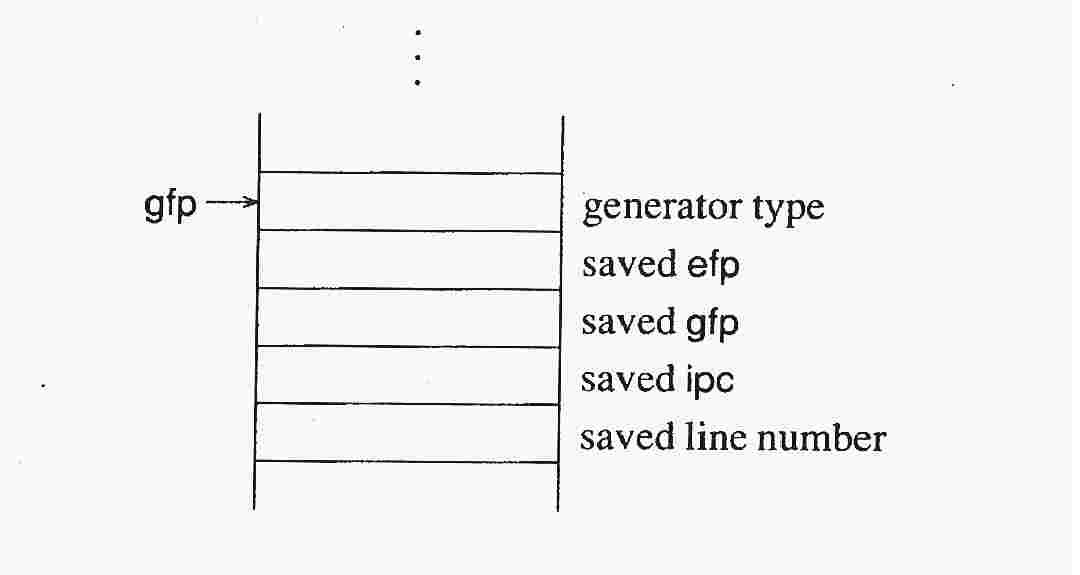
\includegraphics[width=3.6335in,height=1.9193in]{ib-img/ib-img066.jpg} 


The corresponding C structure is

{\ttfamily\mdseries
\ \ \ struct gf\_marker \{\textit{\ \ /* }generator frame marker \textit{*/}}

{\ttfamily\mdseries
\ \ \ \ \ \ word gf\_gentype;\textit{\ \ /*}\ \ type \textit{*/}}

{\ttfamily\mdseries
\ \ \ \ \ \ struct ef\_marker *gf\_efp;\textit{\ \ /*}\ \ efp \textit{*/}}

{\ttfamily\mdseries
\ \ \ \ \ \ struct gf\_marker *gf\_gfp;\textit{\ \ /*}\ \ gfp */}

{\ttfamily\mdseries
\ \ \ \ \ \ word *gf\_ipc;\textit{\ \ /*}\ \ ipc \textit{*/}}

{\ttfamily\mdseries
\ \ \ \ \ \ word gf\_line;\textit{\ \ /*}\ \ line number */}

{\ttfamily\mdseries
\ \ \ \};}


Generators for procedure suspension contain, in addition, the i-state
variable related to procedures. See Sec. 10.3.3.

As an example, consider the expression

{\ttfamily\mdseries
\ \ \ write(i = (1 to 3));}


The virtual machine instructions for this expression are:

{\ttfamily\mdseries
\ \ \ mark L1}

{\ttfamily\mdseries
\ \ \ global write}

{\ttfamily\mdseries
\ \ \ pnull}

{\ttfamily\mdseries
\ \ \ local i}

{\ttfamily\mdseries
\ \ \ int 1}

{\ttfamily\mdseries
\ \ \ int 3}

{\ttfamily\mdseries
\ \ \ push 1\ \ \# default increment}

{\ttfamily\mdseries
\ \ \ toby}

{\ttfamily\mdseries
\ \ \ numeq}

{\ttfamily\mdseries
\ \ \ invoke 1}

{\ttfamily\mdseries
\ \ \ unmark}

{\ttfamily\mdseries
L1 :}


The state of the stack after execution of the first seven instructions is


\ \  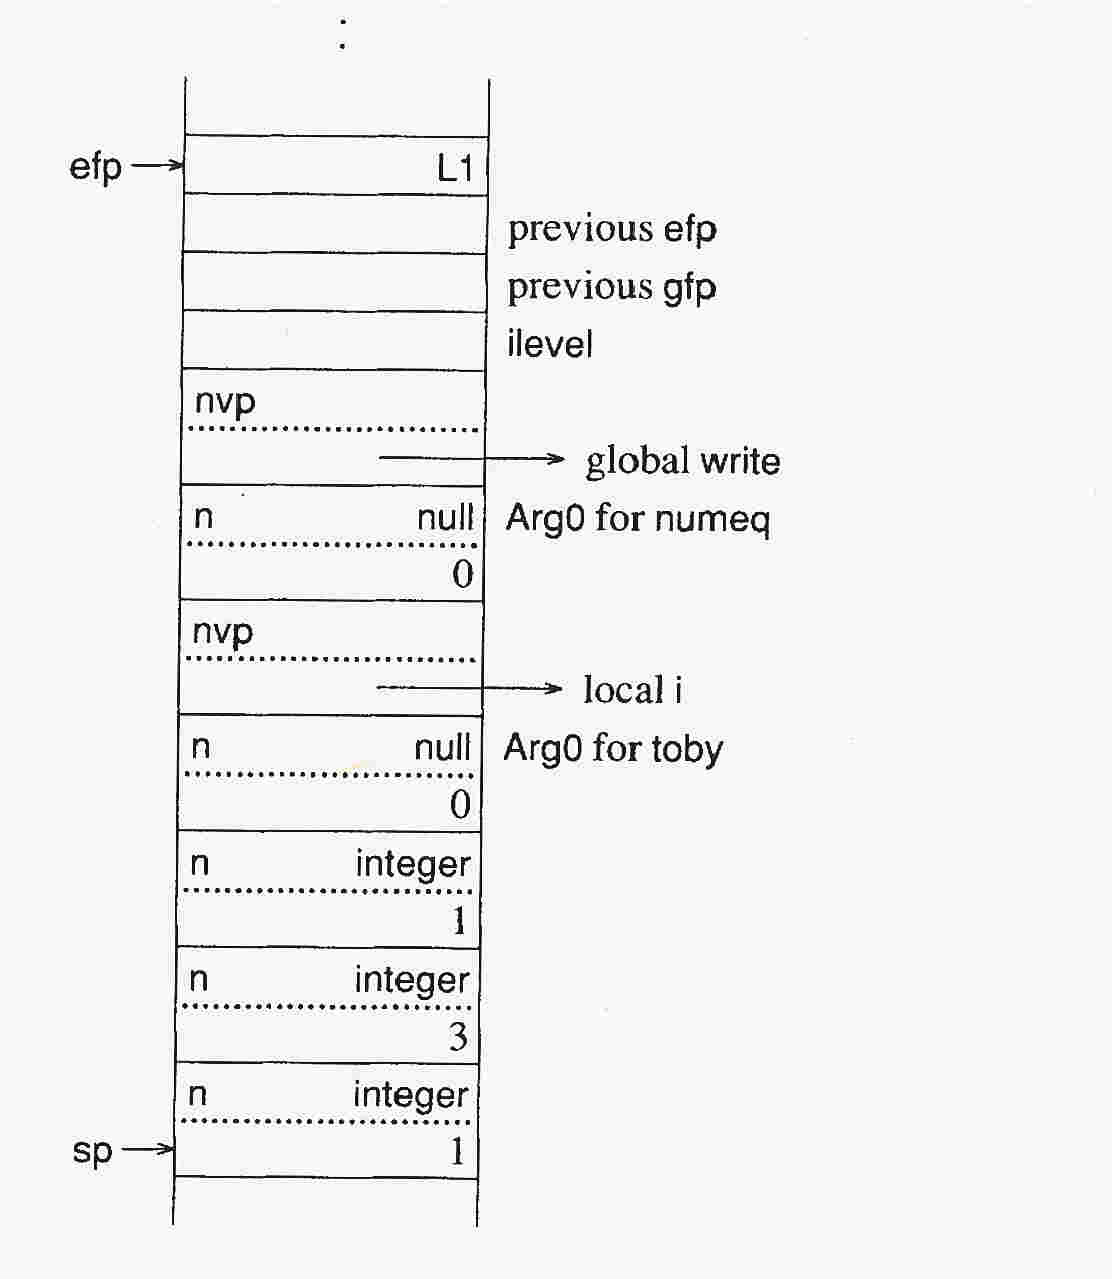
\includegraphics[width=3.7402in,height=4.2717in]{ib-img/ib-img067.jpg} 


The code in the interpreter for calling a generative operator with n
arguments is

{\ttfamily\mdseries
\ \ \ rargp = (struct descrip *)(sp -1) -n;}

{\ttfamily\mdseries
\ \ \ signal = (*(optab[op]))(rargp);}

{\ttfamily\mdseries
\ \ \ goto C\_rtn\_term;}


Note that \texttt{rargp} points to Arg0 and is the argument of the
call to the C function for the operator.

The RTL function for \texttt{toby} is

{\ttfamily\mdseries
operator\{*\} ... toby(from, to, by)}

{\ttfamily\mdseries
\ \ \ /*}

{\ttfamily\mdseries
\ \ \ \ * arguments must be integers.}

{\ttfamily\mdseries
\ \ \ \ */}

{\ttfamily\mdseries
\ \ \ if !cnv:C\_integer(from) then}

{\ttfamily\mdseries
\ \ \ \ \ \ runerr(101, from)}

{\ttfamily\mdseries
\ \ \ if !cnv:C\_integer(to) then}

{\ttfamily\mdseries
\ \ \ \ \ \ runerr(101, to)}

{\ttfamily\mdseries
\ \ \ if !cnv:C\_integer(by) then}

{\ttfamily\mdseries
\ \ \ \ \ \ runerr(101, by)}

{\ttfamily\mdseries
\ \ \ abstract \{}

{\ttfamily\mdseries
\ \ \ \ \ \ return integer}

{\ttfamily\mdseries
\ \ \ \ \ \ \}}

{\ttfamily\mdseries
\ \ \ inline \{}

{\ttfamily\mdseries
\ \ \ \ \ \ /*}

{\ttfamily\mdseries
\ \ \ \ \ \ \ * by must not be zero.}

{\ttfamily\mdseries
\ \ \ \ \ \ \ */}

{\ttfamily\mdseries
\ \ \ \ \ \ if (by == 0) \{}

{\ttfamily\mdseries
\ \ \ \ \ \ \ \ \ irunerr(211, by);}

{\ttfamily\mdseries
\ \ \ \ \ \ \ \ \ errorfail;}

{\ttfamily\mdseries
\ \ \ \ \ \ \ \ \ \}}

{\ttfamily\mdseries
\ \ \ \ \ \ /*}

{\ttfamily\mdseries
\ \ \ \ \ \ \ * Count up or down (depending on relationship of from and}

{\ttfamily\mdseries
\ \ \ \ \ \ \ * \ to) and suspend each value in sequence, failing when}

{\ttfamily\mdseries
\ \ \ \ \ \ \ * \ the limit has been exceeded.}

{\ttfamily\mdseries
\ \ \ \ \ \ \ */}

{\ttfamily\mdseries
\ \ \ \ \ \ if (by {\textgreater} 0)}

{\ttfamily\mdseries
\ \ \ \ \ \ \ \ \ for ( ; from {\textless}= to; from += by) \{}

{\ttfamily\mdseries
\ \ \ \ \ \ \ \ \ \ \ \ suspend C\_integer from;}

{\ttfamily\mdseries
\ \ \ \ \ \ \ \ \ \ \ \ \}}

{\ttfamily\mdseries
\ \ \ \ \ \ else}

{\ttfamily\mdseries
\ \ \ \ \ \ \ \ \ for ( ; from {\textgreater}= to; from += by) \{}

{\ttfamily\mdseries
\ \ \ \ \ \ \ \ \ \ \ \ suspend C\_integer from;}

{\ttfamily\mdseries
\ \ \ \ \ \ \ \ \ \ \ \ \}}

{\ttfamily\mdseries
\ \ \ \ \ \ fail;}

{\ttfamily\mdseries
\ \ \ \ \ \ \}}

{\ttfamily\mdseries
end}

The RTL \texttt{operator} construct, which is similar to
\texttt{function}, produces the C header

{\ttfamily\mdseries
int Otoby(dptr r\_args)}

\noindent so that \texttt{toby} is called with a pointer to
Arg0. Arguments with logical names Arg0, Arg1, and so forth are
referred as \texttt{r\_args[0]}, \texttt{r\_args[1]}, and so on in the
generated code.

When \texttt{toby} is called, it replaces its Arg0 descriptor by a
descriptor for the integer \texttt{from} and suspends by using the RTL
\texttt{suspend} construct rather than \texttt{return}.

The \texttt{suspend} statement \textit{calls }\texttt{interp()}
instead of returning to it. This leaves the call of \texttt{toby}
intact with its variables preserved and also transfers control to
\texttt{interp()} so that the next virtual machine instruction can be
interpreted. However, it is necessary to push a generator marker on
the interpreter stack and copy a portion of the interpreter stack, so
that interpretation can continue without changing the portion of the
interpreter stack that \texttt{toby} needs in case it is resumed. This
is accomplished by calling \texttt{interp()} with arguments that
signal it to build a generator frame. The C code generated for
\texttt{suspend} is

{\ttfamily\mdseries
\ \ \ if ((signal = interp(G\_Osusp, r\_args RTTCURTSTATARG)) !=}

{\ttfamily\mdseries
\ \ \ \ \ \ \ \ A\_Resume) \{}

{\ttfamily\mdseries
\ \ \ \ \ \ return signal;}

{\ttfamily\mdseries
\ \ \ \ \ \ \}}

The argument \texttt{G\_Osusp} in the call of \texttt{interp()}
indicates that a generator frame for C function that implements an
operator is needed. The argument \texttt{r\_args} points to the
location on the interpreter stack where Arg0 for the suspending C
function is located. This location is the same as rargp in the call of
\texttt{interp()} that called upto.

In this situation, \texttt{interp()} puts a generator frame marker on
the interpreter stack and copies the portion of the interpreter stack
from the last expression 01 generator frame marker through cargp onto
the top of the interpreter stack:

\ \  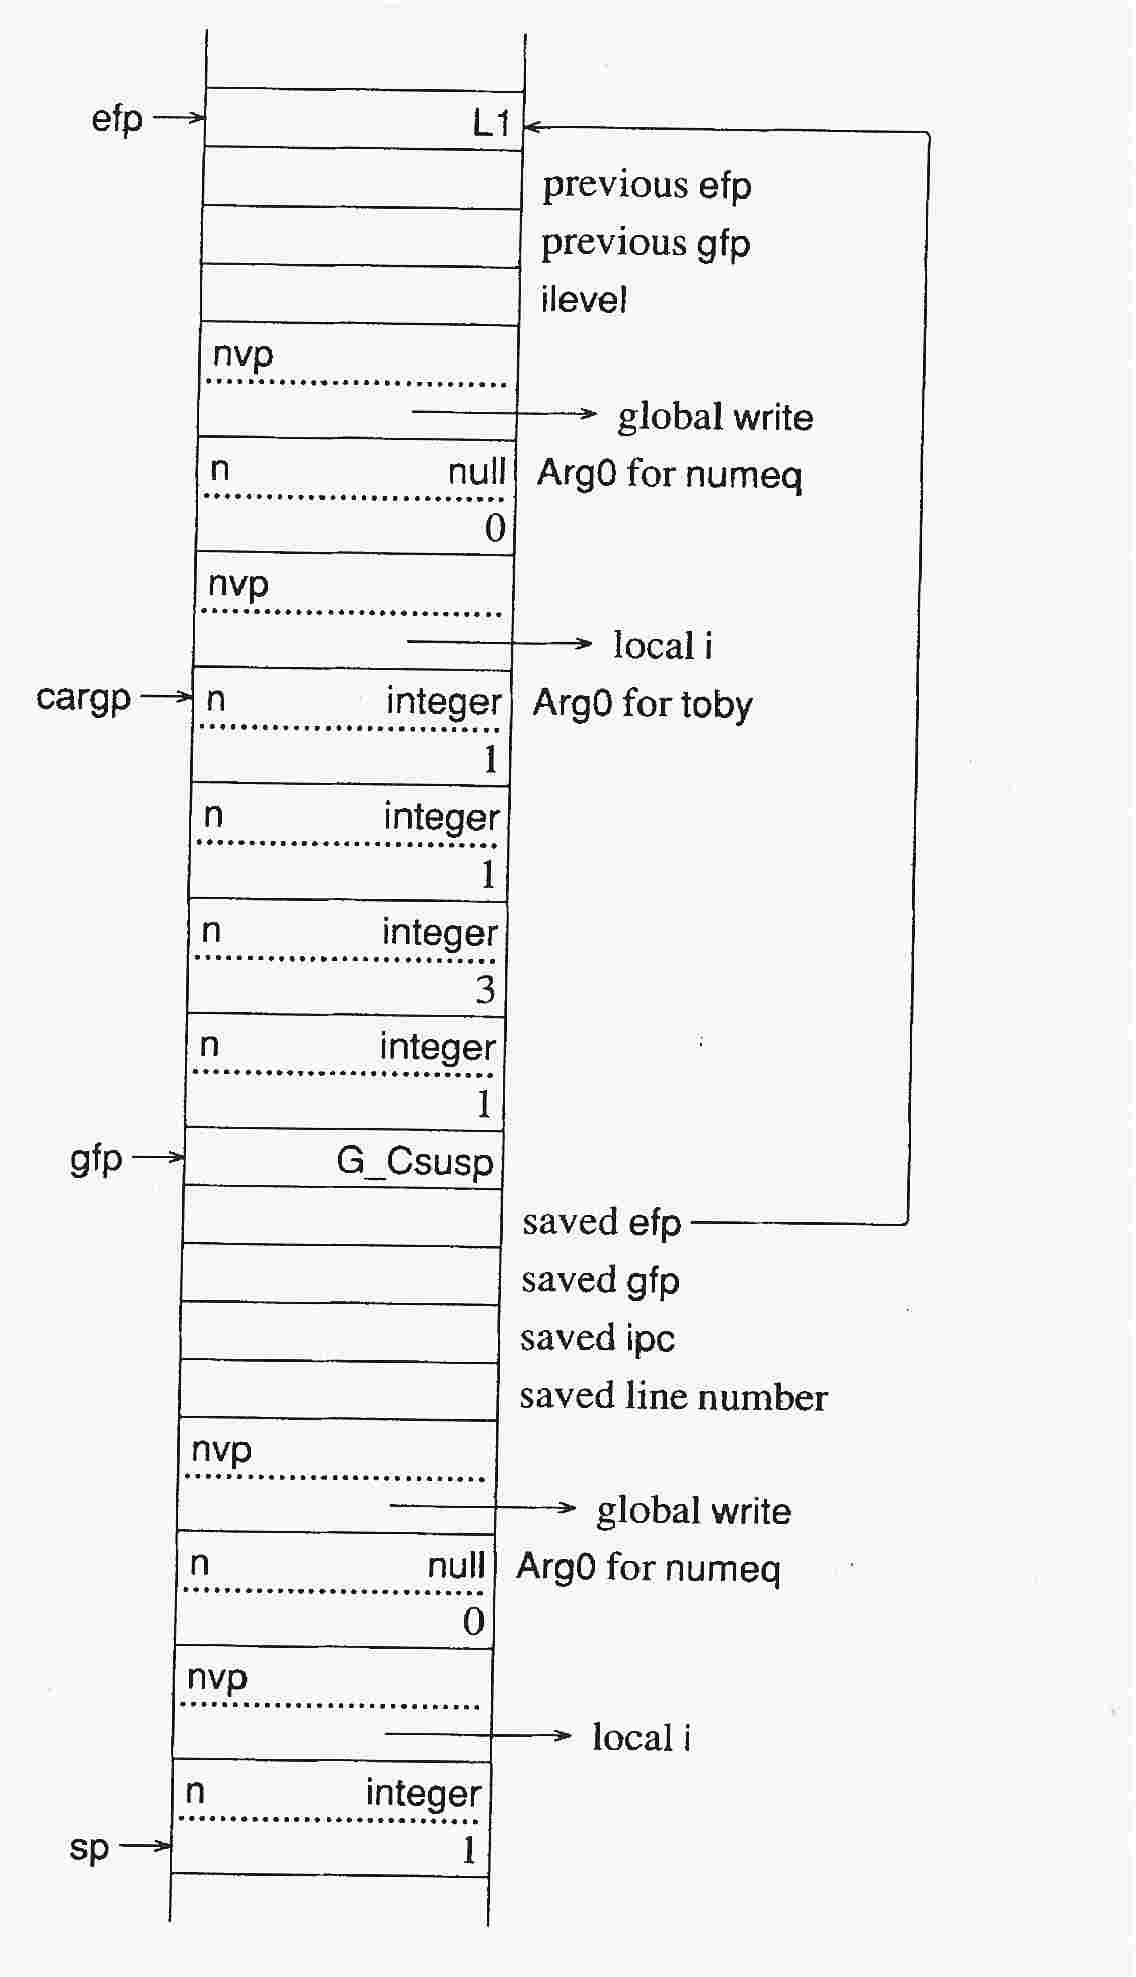
\includegraphics[width=3.848in,height=6.6035in]{ib-img/ib-img068.jpg} 

The stack is exactly the same, as far as the execution of
\texttt{numeq} is concerned, as it would have been if \texttt{toby}
had simply returned. However, the arguments of \texttt{toby} (and the
\ preceding arguments of \texttt{numeq}) are still intact, so that
\texttt{toby} can be resumed. The generator frame is interposed
between the two portions of the interpreter stack. The top of the
stack corresponds to the evaluation of

{\ttfamily\mdseries
\ \ \ write(i = 1);}


\textbf{Resumption}.\ \ Suppose the value of \texttt{i} in the
previous example is 2. The comparison fails and control is transferred
to \texttt{efail}, as it is in the case of all operations that
fail. The code for \texttt{efail} is

{\ttfamily\mdseries
\ \ \ case Op\_Efail:}

{\ttfamily\mdseries
\ \ \ efail:}

{\ttfamily\mdseries
\ \ \ \ \ \ /*}

{\ttfamily\mdseries
\ \ \ \ \ \ \ * Failure has occurred in the current expression frame.}

{\ttfamily\mdseries
\ \ \ \ \ \ \ */}

{\ttfamily\mdseries
\ \ \ \ \ \ if (gfp == 0) \{}

{\ttfamily\mdseries
\ \ \ \ \ \ \ \ \ /*}

{\ttfamily\mdseries
\ \ \ \ \ \ \ \ \ \ * There are no suspended generators to resume. Remove}

{\ttfamily\mdseries
\ \ \ \ \ \ \ \ \ \ * the current expression frame, restoring values.}

{\ttfamily\mdseries
\ \ \ \ \ \ \ \ \ \ *}

{\ttfamily\mdseries
\ \ \ \ \ \ \ \ \ \ * If the failure ipc is 0, propagate failure to the}

{\ttfamily\mdseries
\ \ \ \ \ \ \ \ \ \ * enclosing frame by branching back to efail.}

{\ttfamily\mdseries
\ \ \ \ \ \ \ \ \ \ * This happens, for example, in looping control}

{\ttfamily\mdseries
\ \ \ \ \ \ \ \ \ \ * structures that fail when complete.}

{\ttfamily\mdseries
\ \ \ \ \ \ \ \ \ \ */}

{\ttfamily\mdseries
\ \ \ \ \ \ \ \ \ ipc = efp-{\textgreater}ef\_failure;}

{\ttfamily\mdseries
\ \ \ \ \ \ \ \ \ gfp = efp-{\textgreater}ef-9fp;}

{\ttfamily\mdseries
\ \ \ \ \ \ \ \ \ sp = (word *)efp -1;}

{\ttfamily\mdseries
\ \ \ \ \ \ \ \ \ efp = efp-{\textgreater}ef\_efp;}

{\ttfamily\mdseries
\ \ \ \ \ \ \ \ \ if (ipc == 0)}

{\ttfamily\mdseries
\ \ \ \ \ \ \ \ \ \ \ \ goto efail;}

{\ttfamily\mdseries
\ \ \ \ \ \ \ \ \ break;}

{\ttfamily\mdseries
\ \ \ \ \ \ \ \ \ \}}

{\ttfamily\mdseries
\ \ \ \ \ \ else \{}

{\ttfamily\mdseries
\ \ \ \ \ \ \ \ \ /*}

{\ttfamily\mdseries
\ \ \ \ \ \ \ \ \ \ * There is a, generator that can be resumed. Make}

{\ttfamily\mdseries
\ \ \ \ \ \ \ \ \ \ * the stack adjustments and then switch on the}

{\ttfamily\mdseries
\ \ \ \ \ \ \ \ \ \ * type of the generator frame marker.}

{\ttfamily\mdseries
\ \ \ \ \ \ \ \ \ \ */}

{\ttfamily\mdseries
\ \ \ \ \ \ \ \ \ register struct gf\_marker *resgfp = gfp;}

{\ttfamily\mdseries
\ \ \ \ \ \ \ \ \ tvoe = resgfp-{\textgreater}gf gentype;}

{\ttfamily\mdseries
\ \ \ \ \ \ \ \ \ ipc = resgfp-{\textgreater}gf\_ipc;}

{\ttfamily\mdseries
\ \ \ \ \ \ \ \ \ efp = resgfp-{\textgreater}gf\_efp;}

{\ttfamily\mdseries
\ \ \ \ \ \ \ \ \ line = resgfp-{\textgreater}gf\_line;}

{\ttfamily\mdseries
\ \ \ \ \ \ \ \ \ gfp = resgfp-{\textgreater}gf\_gfp;}

{\ttfamily\mdseries
\ \ \ \ \ \ \ \ \ sp = (word * )resgfp -1;}

{\ttfamily\mdseries
\ \ \ \ \ \ \ \ \ switch (type) \{}


\ \ \ \ \ \ \ \ \ case G\_Csusp: \{


\ \ \ \ \ \ \ \ \ \ \ \ {}-{}-ilevel;

{\ttfamily\mdseries
\ \ \ \ \ \ \ \ \ \ \ \ return A\_Resumption;}

{\ttfamily\mdseries
\ \ \ \ \ \ \ \ \ \ \ \ \textrm{break;}}

{\ttfamily\mdseries
\ \ \ \ \ \ \ \ \ \ \ \ \}}

{\ttfamily\mdseries
\ \ \ \ \ \ \ \ \ case G\_Esusp:}

{\ttfamily\mdseries
\ \ \ \ \ \ \ \ \ \ \ \ goto efail;}

{\ttfamily\mdseries
\ \ \ \ \ \ \ \ \ case G\_Psusp:}

{\ttfamily\mdseries
\ \ \ \ \ \ \ \ \ \ \ \ break;}

{\ttfamily\mdseries
\ \ \ \ \ \ \ \ \ \}}

{\ttfamily\mdseries
\ \ \ \ \ \ break;}

{\ttfamily\mdseries
\ \ \ \ \ \ \}}


If there were no generator frame (if \texttt{gfp} were 0), the entire
expression frame would be removed, and the expression would fail as
described in Sec. 9.2. However, since there is a C\_Susp generator
frame, the stack is restored to the state it\ \ is in when
\texttt{toby} suspended, and the values saved in the generator frame
marker are \textit{restored:}


\ \  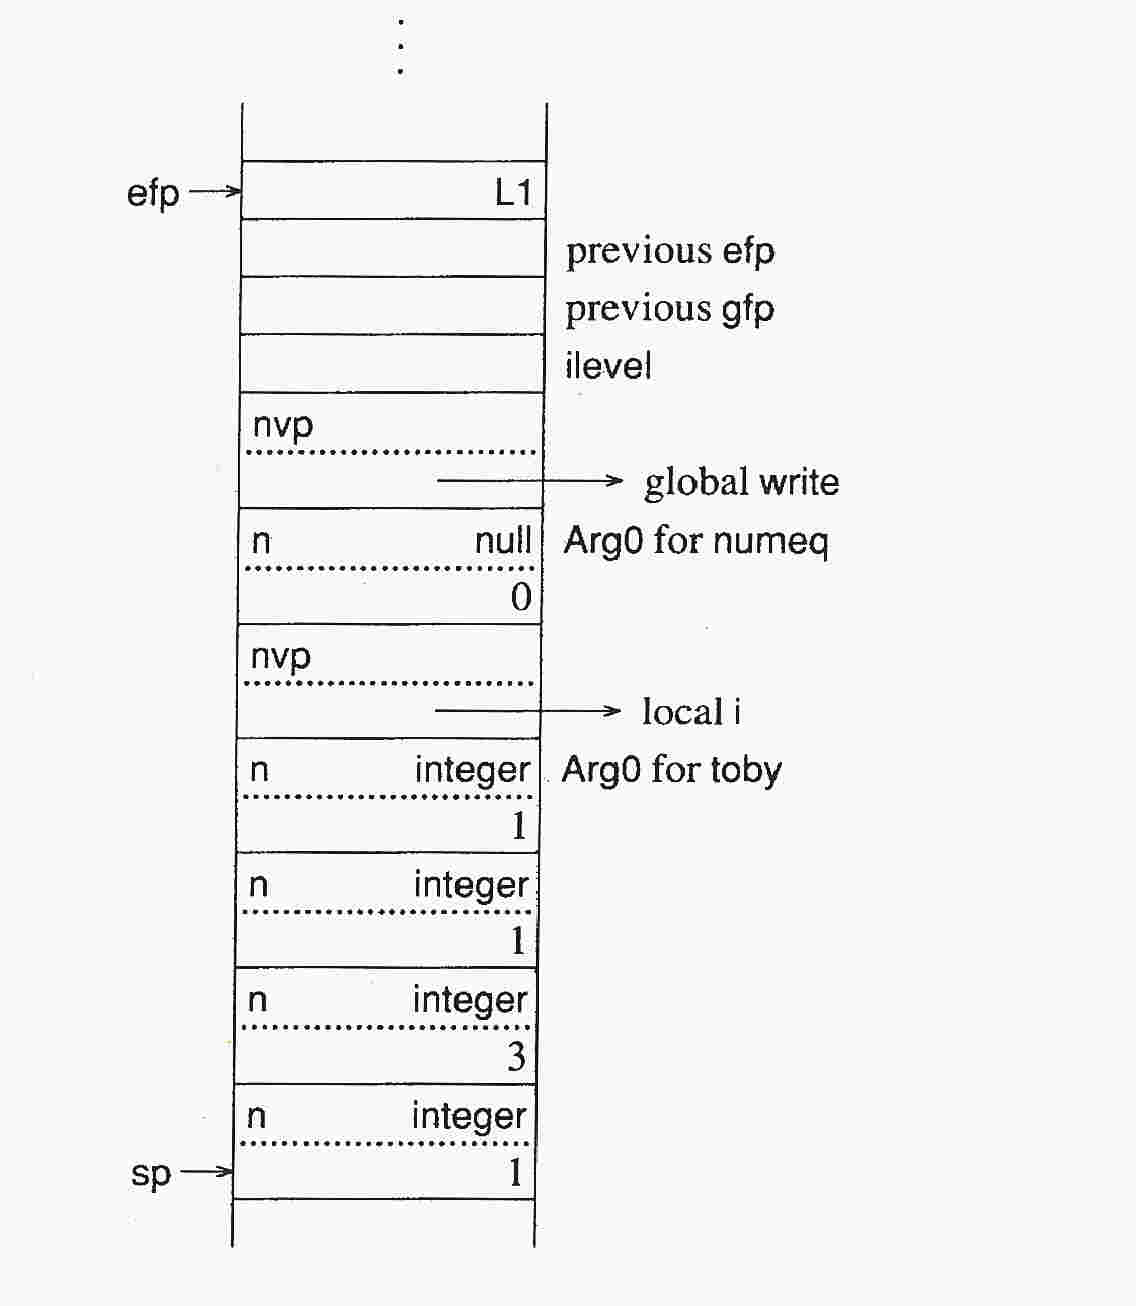
\includegraphics[width=3.848in,height=4.361in]{ib-img/ib-img069.jpg} 


All traces of the first execution of \texttt{numeq} have been removed
from the stack. As shown by the code for \texttt{efail}, the call to
\texttt{toby} is resumed by \textit{returning} to it from
\texttt{interp()} with the signal \texttt{A\_Resumption}, which
indicates another result is needed. When control is returned to
\texttt{toby}, it changes its Arg0 descriptor to the integer 2
suspends again:


\ \  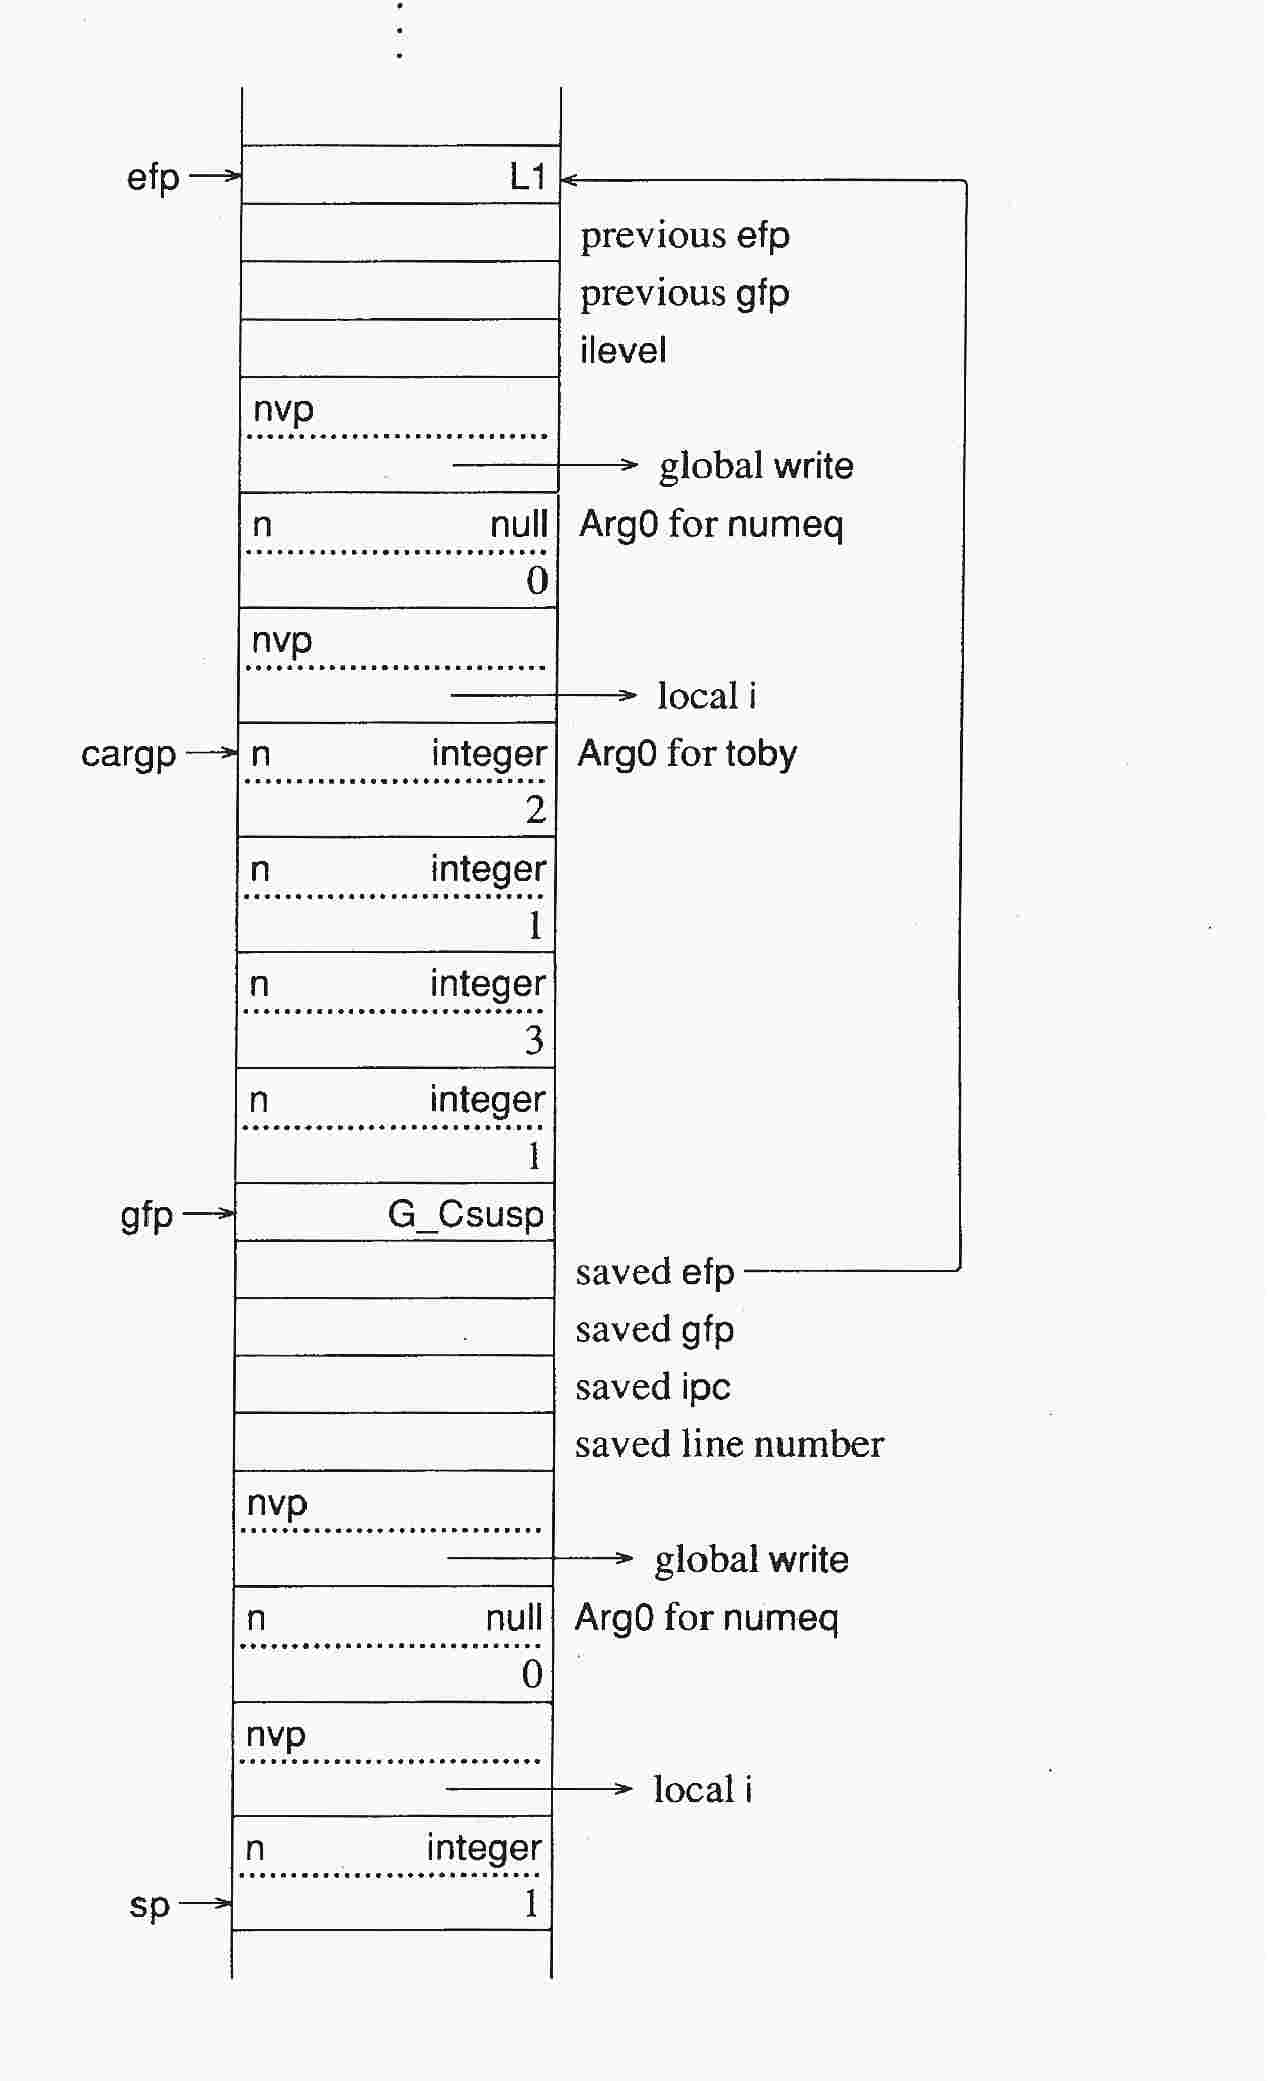
\includegraphics[width=4.2752in,height=6.9508in]{ib-img/ib-img070.jpg} 


The interpreter stack is exactly as it was when \texttt{toby}
suspended the first time, except that the integer 2 is on the stack in
place of the integer 1. The top of the stack corresponds to the
evaluation of

{\ttfamily\mdseries
\ \ \ write(i = 2);}


Since the value of \texttt{i} is 2, \texttt{numeq} succeeds. It copies
the value of its second argument to its Arg0 descriptor and
returns. The value 2 is written and the \texttt{unmark} instruction is
executed, removing the entire expression frame from the stack.


\textbf{Goal-Directed Evaluation. }Goal-directed evaluation occurs
when an expression fails and there are generator frames on the
interpreter stack as the consequence of expressions that have
suspended.

In the case of an expression such as

{\ttfamily\mdseries
\ \ \ 1 to upto(c, s)}

\noindent \texttt{upto()} suspends first, followed by
\texttt{toby}. These generator frames are linked together, with
\texttt{gfp} pointing to the one for \texttt{toby}, which in turn
contains a pointer to the one for \texttt{upto()}. In general,
generator frames are linked together with \texttt{gfp} pointing to the
one for the most recent suspension. This produces the last-in,
first-out (depth-first) \textit{order of} expression evaluation in
Icon. Goal-directed evaluation occurs as a result of resuming
a suspended expression when failure occurs in the surrounding
expression frame.


\textbf{Removing C Frames.} Since C functions that suspend call the
interpreter and the interpreter in turn calls C functions, expression
evaluation typically results in a sequence of frames for calls on the
C stack. When the evaluation of a bounded expression is complete,
there may be frames on the C stack for generators, even though these
generators no longer can be resumed.

In order to {\textquotedbl}unwind{\textquotedbl} the C stack in such
cases, the i-state variable \texttt{ilevel} is used to keep track of
the level of call of \texttt{interp()} by C functions. Whenever
\texttt{interp()} is called, it increments \texttt{ilevel}. When an
expression frame is created, the current value of \texttt{ilevel} is
saved in it, as illustrated previously.

When the expression frame is about to be removed, if the current value
of \texttt{ilevel} is greater than the value in the current expression
frame, \texttt{ilevel} is decremented and the interpreter
\textit{returns }with a signal to the C function that called it to
return rather than to produce another result. If the signal returned
by \texttt{interp()} is \texttt{A\_Resumption}, the C function
continues execution, while for any other signal the C function
returns.

Since C functions return to \texttt{interp()}, \texttt{interp()}
always checks the signal returned to it to determine if it produced a
result or if it is unwinding. If it is unwinding, \texttt{interp()}
returns the unwinding signal instead of continuing evaluation
of\textit{ }the current expression.

Consider again the expression

{\ttfamily\mdseries
\ \ \ write(i = (1 to 3));}

\noindent for which the virtua1 machine instructions are

{\ttfamily\mdseries
\ \ \ mark L1}

{\ttfamily\mdseries
\ \ \ global write}

{\ttfamily\mdseries
\ \ \ pnull}

{\ttfamily\mdseries
\ \ \ local i}

{\ttfamily\mdseries
\ \ \ int 1}

{\ttfamily\mdseries
\ \ \ int 3}

{\ttfamily\mdseries
\ \ \ push1\ \ \# default increment}

{\ttfamily\mdseries
\ \ \ toby}

{\ttfamily\mdseries
\ \ \ numeq}

{\ttfamily\mdseries
\ \ \ invoke 1}

{\ttfamily\mdseries
\ \ \ unmark}

{\ttfamily\mdseries
L1 :}


When \texttt{toby} produces a result, it calls \texttt{interp()}. When
the \texttt{unmark} instruction is executed, the C stack contains a
frame for the call to \texttt{toby} and for its call to
\texttt{interp()}. The code for \texttt{unmark} is

{\ttfamily\mdseries
\ \ \ case Op\_Unmark:\ \ /* remove expression frame */}

{\ttfamily\mdseries
\ \ \ \ \ \ gfp = efp-{\textgreater}ef-9fp;}

{\ttfamily\mdseries
\ \ \ \ \ \ sp = (word *)efp -1;}

{\ttfamily\mdseries
\ \ \ \ \ \ /*}

{\ttfamily\mdseries
\ \ \ \ \ \ \ * Remove any suspended C generators.}

{\ttfamily\mdseries
\ \ \ \ \ \ \ */}

{\ttfamily\mdseries
\ \ \ Unmark\_uw:}

{\ttfamily\mdseries
\ \ \ \ \ \ if (efp-{\textgreater}ef\_ilevel {\textless} ilevel) \{}

{\ttfamily\mdseries
\ \ \ \ \ \ \ \ \ {}-{}-ilevel;}

{\ttfamily\mdseries
\ \ \ \ \ \ \ \ \ return A\_Unmark\_uw;}

{\ttfamily\mdseries
\ \ \ \ \ \ \ \ \ \}}

{\ttfamily\mdseries
\ \ \ \ \ \ efp = efp-{\textgreater}ef\_efp;}

{\ttfamily\mdseries
\ \ \ \ \ \ break;}

Note that in this case Suspend gets the return code
\texttt{A\_Unmark\_uw} and in turn returns \texttt{A\_Unmark\_uw} to
\texttt{interp()}. The section of code in \texttt{interp()} that
checks the signal that is returned from C functions is

{\ttfamily\mdseries
\ \ \ C\_rtn\_term:}

{\ttfamily\mdseries
\ \ \ \ \ \ switch (signal) \{}

{\ttfamily\mdseries
\ \ \ \ \ \ case A\_Failure:}

{\ttfamily\mdseries
\ \ \ \ \ \ \ \ \ goto efail;}

{\ttfamily\mdseries
\ \ \ \ \ \ case A\_Unmark\_uw:\ \ /* unwind for unmark */}

{\ttfamily\mdseries
\ \ \ \ \ \ \ \ \ goto Unmark uw;}

{\ttfamily\mdseries
\ \ \ \ \ \ case A\_Lsusp\_uw:\ \ /* unwind for Isusp */}

{\ttfamily\mdseries
\ \ \ \ \ \ \ \ \ goto Lsusp\_uw;}

{\ttfamily\mdseries
\ \ \ \ \ \ case A\_Eret\_uw:\ \ /* unwind for eret */}

{\ttfamily\mdseries
\ \ \ \ \ \ \ \ \ goto Eret\_uw;}

{\ttfamily\mdseries
\ \ \ \ \ \ case A\_Pret\_uw:\ \ /* unwind for pret */}

{\ttfamily\mdseries
\ \ \ \ \ \ \ \ \ goto Pret\_uw;}

{\ttfamily\mdseries
\ \ \ \ \ \ case A\_Pfail\_uw:\ \ /* unwind for pfail */}

{\ttfamily\mdseries
\ \ \ \ \ \ \ \ \ goto Pfail\_uw;}

{\ttfamily\mdseries
\ \ \ \ \ \ \}}

{\ttfamily\mdseries
\ \ \ \ \ \ sp = (word * )rargp + 1;\ \ /* set sp to result */}

{\ttfamily\mdseries
\ \ \ \ \ \ continue;}

{\ttfamily\mdseries
\ \ \ \}}


Thus, when \texttt{interp()} returns to a C function with an unwinding
signal, there is a cascade of C returns until \texttt{ilevel} is the
same as it was when the current expression frame was created. Note
that there are several cases in addition to \texttt{unmark} where
unwinding is necessary.

\section[9.4 Generative Control Structures]{9.4 Generative Control Structures}

In addition to functions and operators that may generate more than one
result, there are several generative control structures at the level
of virtual machine instructions.

\subsection[9.4.1 Alternation]{9.4.1 Alternation}

The virtual machine instructions for

{\ttfamily\mdseries
\ \ \ \ \ \ \textit{expr\TextSubscript{2}} {\textbar} \textit{expr\TextSubscript{3}}}

are

{\ttfamily\mdseries
\ \ \ mark L1}

{\ttfamily\itshape
\ \ \ code for expr\TextSubscript{2}}


\textit{\ \ \ }esusp

{\ttfamily\mdseries
\ \ \ goto L2}

{\ttfamily\mdseries
L1:}

{\ttfamily\mdseries
\ \ \ \textit{code for expr}\textit{\TextSubscript{3}}}

{\ttfamily\mdseries
L2:}


The mark instruction creates an expression frame marker for
alternation whose purpose is to preserve the failure \texttt{ipc} for
\texttt{L1} in case the results for \textit{expr3 }are needed. If
\textit{expr2 }produces a result, \texttt{esusp} creates a generator
frame with the usual marker and then copies the portion of the
interpreter stack between the last expression or generator frame
marker and the alternation marker to the top of the stack. It then
pushes a copy of the result produced by \textit{expr2}. This connects
the result produced by \textit{expr2 }with the expression prior to the
alternation control structure. Next, \texttt{esusp} sets \texttt{efp}
to point to the expression frame marker prior to the alternation
marker. For example, in the expression

{\ttfamily\mdseries
\ \ \ write(i := 1 {\textbar} 2)}

\noindent the stack after the execution of \texttt{esusp} is


\ \  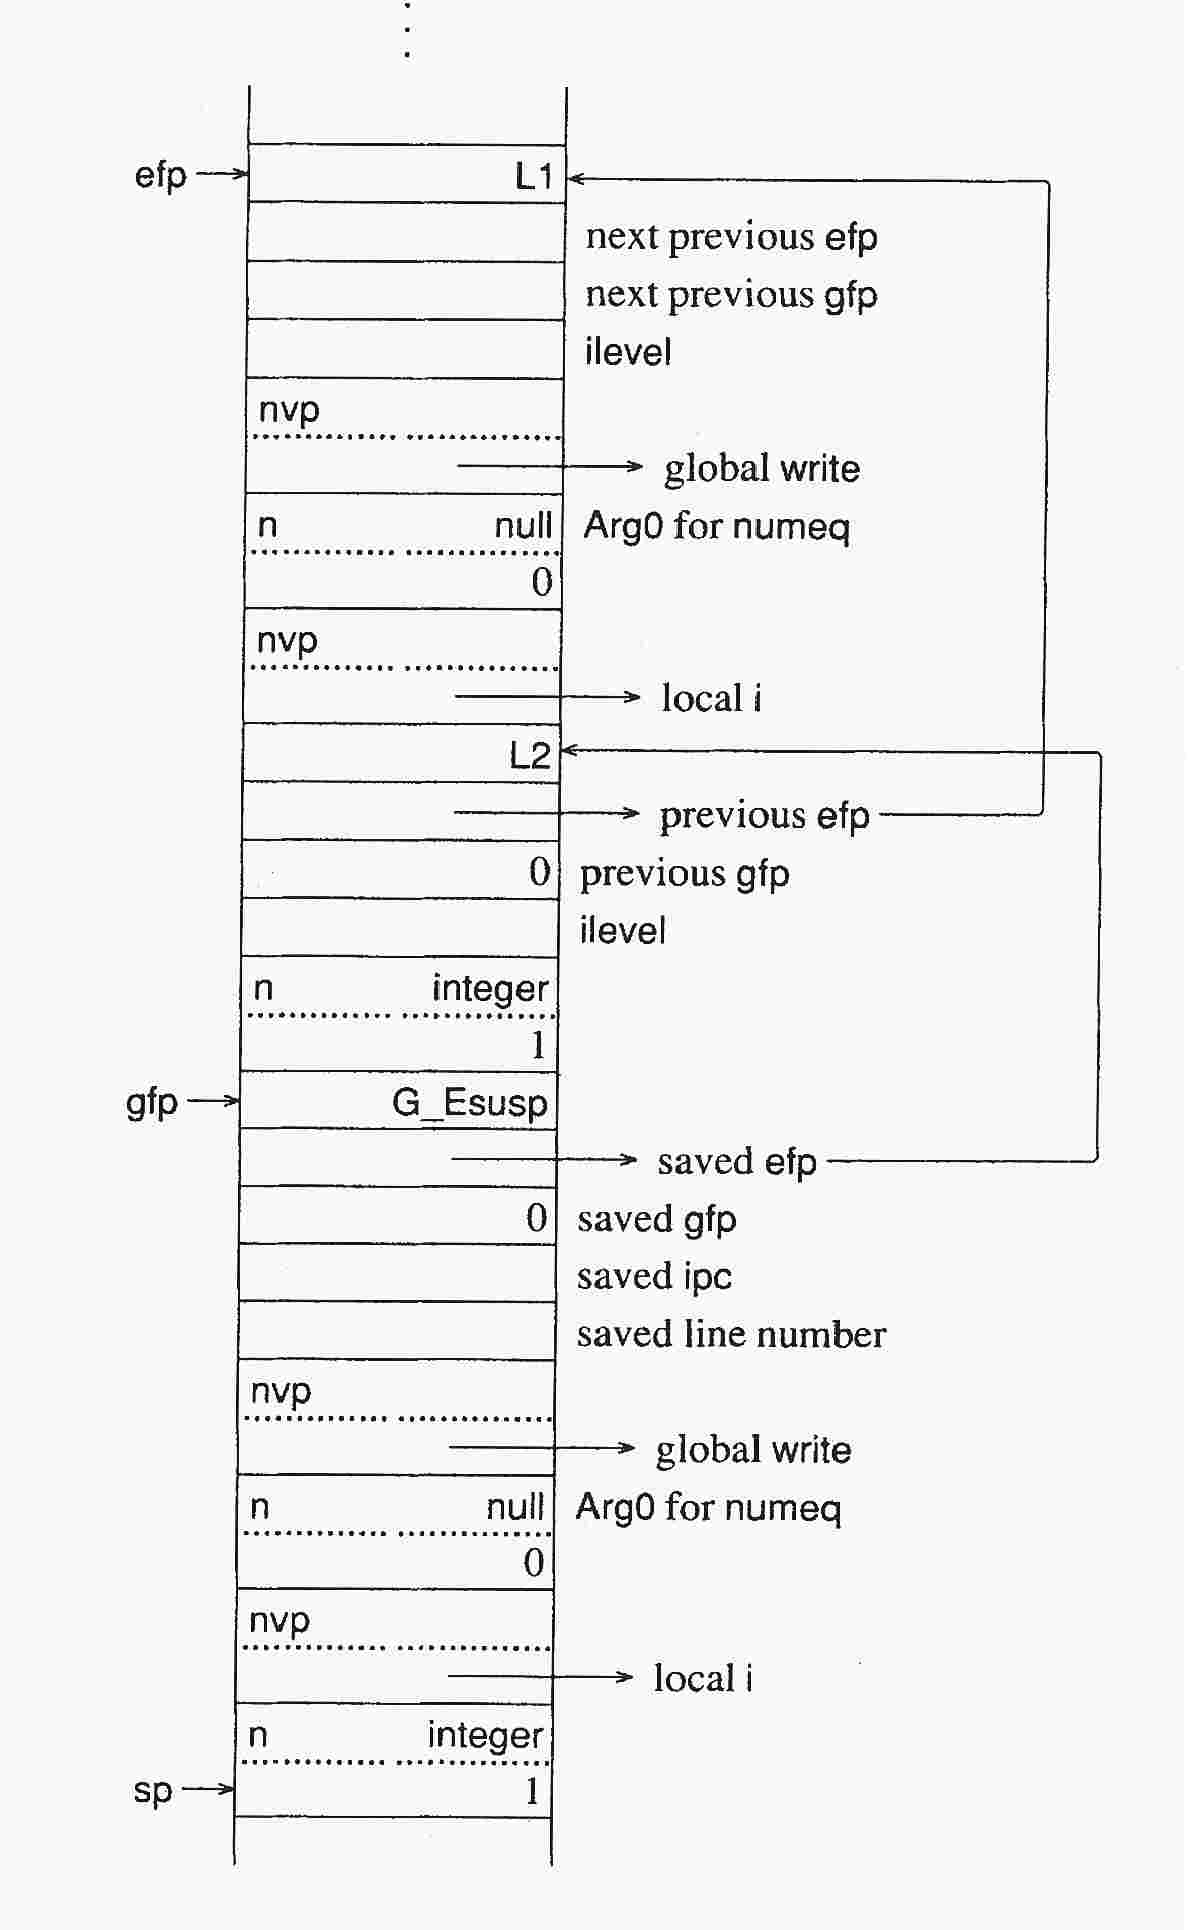
\includegraphics[width=4.0602in,height=6.4457in]{ib-img/ib-img071.jpg} 


The top portion of the stack is the same as if \textit{expr2 }had
produced a result in the absence of alternation.  However, the
generator frame marker pushed by \texttt{esusp} contains a pointer to
the alternation marker.

If another result from \textit{expr2} is needed, the generator frame
left by \texttt{esusp} is removed, restoring the stack to its state
when \textit{expr2} produced a result. If \textit{expr2} itself was a
generator that suspended, it is resumed. Otherwise, control is
transferred to \texttt{efail} and \texttt{ipc} is set to a value
corresponding to \texttt{L1}, so that \textit{expr3} is evaluated next.

\subsection[9.4.2 Repeated Alternation]{9.4.2 Repeated Alternation}

Alternation is the general model for generative control
structures. Repeated alternation, \texttt{{\textbar}}\textit{expr}, is
similar to alternation, and would be equivalent to

{\ttfamily\mdseries
\textit{\ \ expr }{\textbar} \textit{expr }{\textbar} \textit{expr }{\textbar} ...}

\noindent except for a special termination condition that causes
repeated alternation to stop if \textit{expr} does not produce a
result. Without this termination condition, an expression such as

{\ttfamily\mdseries
\ \ \ \ \ {\textbar}upto(c, s)}

\noindent would never return if \texttt{upto()} failed--expression
evaluation would vanish into a {\textquotedbl}black
hole.{\textquotedbl} Expressions that produce results at one time but
not at another also are useful. For example,

{\ttfamily\mdseries
\ \ \ \ \ {\textbar}read()}

\noindent generates the lines from the standard input file. Because of
the termination condition, this expression terminates when the end of
the input file is reached. If it vanished into a {\textquotedbl}black
hole,{\textquotedbl} it could not be used safely.

If it were not for the termination condition, the virtual machine
instructions for \texttt{{\textbar}}\textit{expr} would be

{\ttfamily\mdseries
L1:}

{\ttfamily\mdseries
\ \ \ \ \ \ mark L1}

{\ttfamily\mdseries
\ \ \ \ \ \ \textit{code for expr}}

{\ttfamily\mdseries
\ \ \ \ \ \ esusp}


The {\textquotedbl}black hole{\textquotedbl} here is evident---if
\textit{expr} fails, it is evaluated again and there is no way out.

The termination condition is handled by an instruction that changes
the failure \texttt{ipc} in the current expression marker. The actual
virtual machine instructions for \texttt{{\textbar}}\textit{expr} are

{\ttfamily\mdseries
L1:}

{\ttfamily\mdseries
\ \ \ \ \ \ mark0}

{\ttfamily\mdseries
\ \ \ \ \ \ code for expr}

{\ttfamily\mdseries
\ \ \ \ \ \ chfail\ \ L1}

{\ttfamily\mdseries
\ \ \ \ \ \ esusp}


The virtual machine instruction \texttt{mark0} pushes an expression
frame marker with a zero failure \texttt{ipc}. If a zero failure
\texttt{ipc} is encountered during failure, as illustrated by the code
for \texttt{efail} in Sec. 9.3, failure is transmitted to the
enclosing expression. If \textit{expr }produces a result, however, the
\texttt{chfail} instruction is executed. It changes the failure
\texttt{ipc} in the current expression marker to correspond to
\texttt{L1}, so that if \textit{expr }does not produce a result when
it is resumed, execution starts at the location in the icode
corresponding to \texttt{L1} again, causing another iteration of the
alternation loop. It is important to realize that \texttt{chfail} only
changes the failure \texttt{ipc} in the current expression marker on
the stack.  Subsequent execution of \texttt{mark0} creates a new
expression frame whose marker has a zero failure \texttt{ipc}.

\subsection[9.4.3 Limitation]{9.4.3 Limitation}

In the limitation control structure,

{\ttfamily\mdseries
\textit{\ \ \ expr1 }{\textbackslash} \textit{expr2}}

\noindent the normal left-to-right evaluation of Icon is reversed and
\textit{expr2 }is evaluated first. The virtual machine instructions are

{\ttfamily\mdseries
\ \ \ \ \ \ \textit{code for expr2}}

{\ttfamily\mdseries
\ \ \ \ \ \ limit}

{\ttfamily\mdseries
\ \ \ \ \ \ \textit{code for expr1}}

{\ttfamily\mdseries
\ \ \ \ \ \ lsusp}

If \textit{expr2 }succeeds, its result is on the top of the stack. The
limit instruction checks this result to be sure that it is legal---an
integer greater than or equal to zero. If it is not an integer, an
attempt is made to convert it to one. If the limit value is zero,
limit fails. Otherwise, limit creates an expression frame marker with
a zero failure \texttt{ipc} and execution continues, so that
\textit{expr1 }is evaluated in its own expression frame. During the
evaluation of \textit{expr1, }the limit value is directly below its
expression marker. For example, in

{\ttfamily\mdseries
\textit{\ \ expr1 }{\textbackslash} 10}

\noindent the stack prior to the evaluation of \textit{expr1} is

\bigskip

If \textit{expr1} produces a result, \texttt{lsusp} is executed. The
\texttt{lsusp} instruction is very similar to \texttt{esusp}. Before
producing a generator frame, however, \texttt{lsusp} decrements the
limit value. If it becomes zero, the expression frame for
\textit{expr1} is removed, the C stack is unwound, and the last value
it produced is placed on the stack in place of the limit
value. Otherwise, it copies the portion of the interpreter stack
between the end of the last expression or generator frame marker and
the limit value to the top of the stack. Note that no generator frame
is needed.

\section[9.5 Iteration]{9.5 Iteration}

The difference between evaluation and resumption in a loop is
illustrated by the virtual machine instructions for a conventional
loop

{\ttfamily\mdseries
\ \ \ while \textit{expr1 }do \textit{expr2}}

and the iteration control structure

{\ttfamily\mdseries
\ \ \ every \textit{expr1 }do \textit{expr2}}

The instructions for \texttt{while-do} are

{\ttfamily
L1:}

{\ttfamily
\ \ mark0}

{\ttfamily
\textit{\ \ code for expr1\newline
\ \ }unmark}

{\ttfamily
\ \ mark L1\newline
\ \ \textit{code for expr2\newline
\ \ }unmark}

{\ttfamily
\ \ goto\ \ L1}

If \textit{expr1} fails, the entire expression fails and failure is
transmitted to the enclosing expression frame because the failure
\texttt{ipc} is zero. If \textit{expr1} produces a result,
\textit{expr2} is evaluated in a separate expression frame. Whether
\textit{expr2} produces a result or not, its expression frame is
removed and execution continues at the beginning of the loop.

The instructions for \texttt{every-do} are

{\ttfamily\mdseries
\ \ mark0}

{\ttfamily\mdseries
\ \ code for expr1}

{\ttfamily\mdseries
\ \ pop}

{\ttfamily\mdseries
\ \ mark0}

{\ttfamily\mdseries
\ \ code for expr2}

{\ttfamily\mdseries
\ \ unmark}

{\ttfamily\mdseries
\ \ efail}


If \textit{expr1} fails, the entire expression fails and failure is
transmitted to the enclosing expression frame as in the case of
\texttt{while-do}. If \textit{expr1} produces a result, it is
discarded by the \texttt{pop} instruction, since this result is not
used in any subsequent computation. The expression frame for
\textit{expr1} is not removed, however, and \textit{expr2} is
evaluated in its own expression frame within the expression frame for
\textit{expr1} (unlike the case for the while loop). If \textit{expr2}
produces a result, its expression frame is removed and \texttt{efail}
is executed. If \textit{expr2} fails, it transmits failure to the
enclosing expression frame, which is the expression frame for
\textit{expr1}. If \textit{expr2} produces a result, \texttt{efail}
causes failure in the expression frame for \textit{expr1}. Thus, the
effect is the same, whether or not \textit{expr2} produces a
result. All results are produced simply by forcing failure.

If the expression frame for \textit{expr1} contains a generator frame,
which is the case if \textit{expr1} suspended, evaluation is resumed
accordingly, so that \textit{expr1} can produce another result. If
\textit{expr1} simply produces a result instead of suspending, there
is no generator frame, \texttt{efail} removes its expression frame,
and failure is transmitted to the enclosing expression frame.


\section[9.6 String Scanning]{9.6 String Scanning}

String scanning is one of the most useful operations in Icon. Its
implementation, however, is comparatively simple.  There is no special
expression-evaluation mechanism associated with string scanning
\textit{per se}; all {\textquotedbl}pattern matching{\textquotedbl}
follows naturally from goal-directed evaluation.

The string-scanning keywords, \texttt{\&subject} and \texttt{\&pos}
must be handled properly, however. These keywords have global scope
with respect to procedure invocation, but they are maintained in a
stack-like fashion with respect to string-scanning expressions.

The expression

{\ttfamily\mdseries
\textit{\ \ expr1 }? \textit{expr2}}

\noindent is a control structure, not an operation, since, by
definition, the arguments for ar operation are evaluated before the
operation is performed. This form of evaluation does not work for
string scanning, since after \textit{expr1} is evaluated, but before
\textit{expr2} is evaluated, the previous values of \texttt{\&subject}
and \texttt{\&pos} must be saved and new ones
established. Furthermore, when string scanning is finished, the old
values of \texttt{\&subject} and \texttt{\&pos} must be restored. In
addition, if string scanning succeeds, the values of these keywords at
the time string scanning produces a result must be saved so that they
can be restored if the string-scanning operation is resumed to produce
another result.

The virtual machine instructions for

{\ttfamily\mdseries
\textit{\ \ expr1 }? \textit{expr2}}

are

{\ttfamily\mdseries
\ \ code for expr1}

{\ttfamily\mdseries
\ \ bscan}

{\ttfamily\mdseries
\ \ code for expr2}

{\ttfamily\mdseries
\ \ escan}

If \textit{expr1} succeeds, it leaves a result on the top of the
stack. The \texttt{bscan} instruction assures that this value is a
string, performing a conversion if necessary. Otherwise, the old
values of \texttt{\&subject} and \texttt{\&pos} are pushed on the
stack, the value of \texttt{\&subject} is set to the (possibly
converted) one produced by \textit{expr1}, and \texttt{\&pos} is set
to 1.


The \texttt{bscan} instruction then suspends. This is necessary in
case \textit{expr2} fails, so that \texttt{bscan} can get control
again to perform data backtracking, restoring the previous values of
\texttt{\&subject} and \texttt{\&pos} from the stack where they were
saved.


If \textit{expr2} succeeds, the \texttt{escan} instruction copies the
descriptor on the top of the stack to its Arg0 position, overwriting
the result produced by \textit{expr2}. It then exchanges the current
values of \texttt{\&subject} and \texttt{\&pos} with those saved by
\texttt{bscan} thus restoring the values of these keywords to their
values prior to the scanning expression and at the same time saving
the values they had at the time \textit{expr2} produced a result. The
\texttt{escan} instruction then suspends.

If \texttt{escan} is resumed, the values of \texttt{\&subject} and
\texttt{\&pos} are restored from the stack, restoring the situation to
what it was when \textit{expr2} produced a result. The \texttt{escan}
instruction then fails in order to force the resumption of any
suspended generators left by \textit{expr2.}

Suppose, for example, that the values of \texttt{\&subject} and
\texttt{\&pos} are \texttt{{\textquotedbl}the{\textquotedbl}} and 2
respectively, when the following expression is evaluated:

{\ttfamily\mdseries
\ \ read(f) ? move(4)}

Suppose \texttt{read(f)} produces the string
\texttt{{\textquotedbl}coconuts{\textquotedbl}}. The stack is

\ \  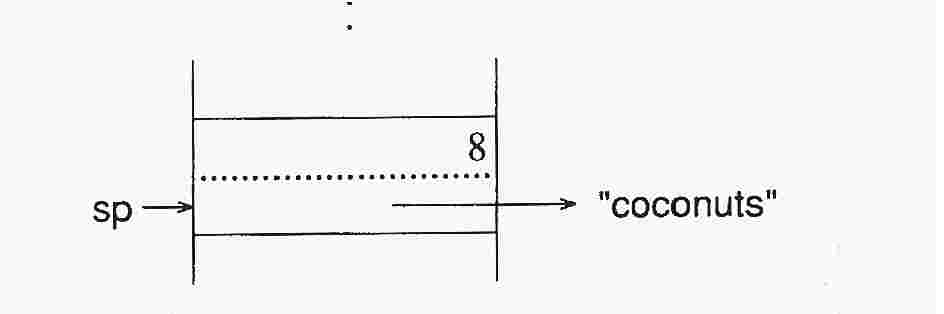
\includegraphics[width=3.2063in,height=1.048in]{ib-img/ib-img072.jpg} 

{\ttfamily\mdseries
\&subject: {\textquotedbl}the{\textquotedbl}\newline
\&pos: 2}

The \texttt{bscan} instruction is executed, pushing the current values
of \texttt{\&subject} and \texttt{\&pos}:

{\sffamily
\ \  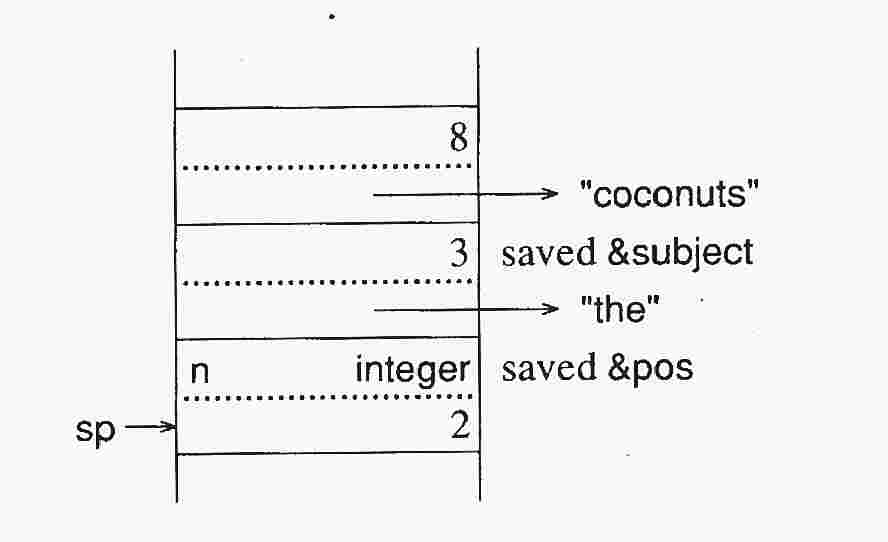
\includegraphics[width=2.9925in,height=1.8098in]{ib-img/ib-img073.jpg} }

{\ttfamily\mdseries
\&subject: {\textquotedbl}the{\textquotedbl}}

{\ttfamily\mdseries
\&pos: 2}

The \texttt{bscan} instruction sets \texttt{\&subject} to
\texttt{{\textquotedbl}coconuts{\textquotedbl}} and \texttt{\&pos} to
1. The \texttt{bscan} instruction then suspends and \texttt{move(4)}
is evaluated. It suspends, and the top I

\ \  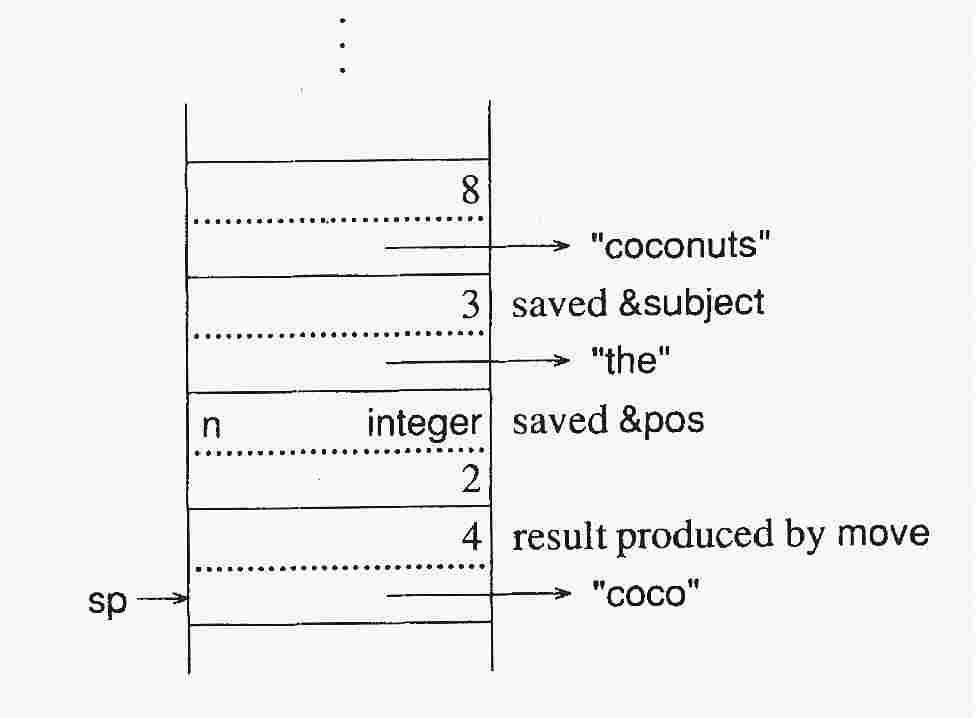
\includegraphics[width=3.3134in,height=2.398in]{ib-img/ib-img074.jpg} 

{\ttfamily\mdseries
\&subject: {\textquotedbl}coconuts{\textquotedbl}\newline
\&pos: 5}

The \texttt{escan} instruction is executed next. It copies the
descriptor on the top of the stack to replace the result produced by
\textit{expr2. }It then exchanges the current values of
\texttt{\&subject} and \texttt{\&pos} with those on the stack:

\ \  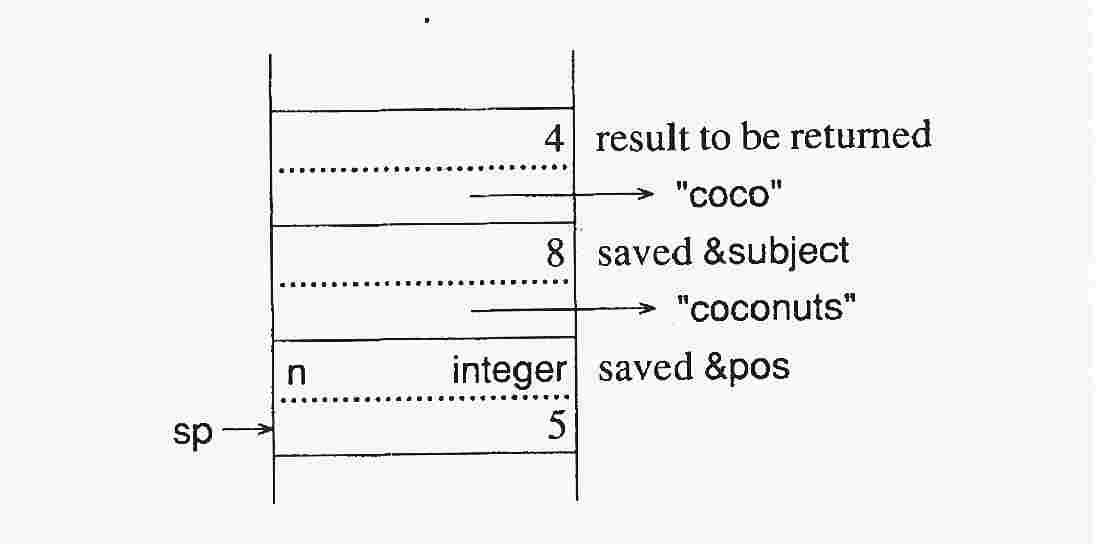
\includegraphics[width=3.7402in,height=1.8161in]{ib-img/ib-img075.jpg} 

{\ttfamily\mdseries
\&subject: {\textquotedbl}the{\textquotedbl}\newline
\&pos: 2}

The \texttt{escan} instruction then suspends, building a generator
frame. The result of \textit{expr2} is placed on the top of the stack,
becoming the result of the entire scanning expression.

\ \  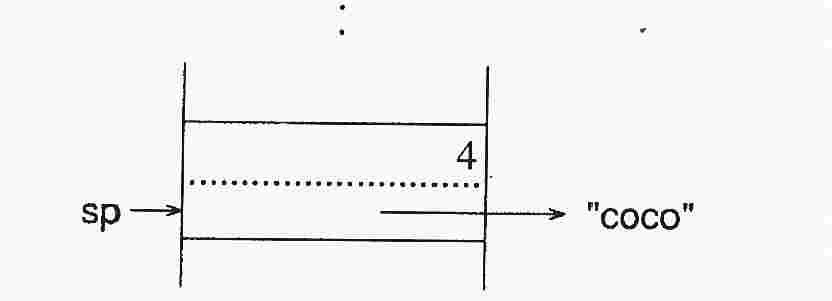
\includegraphics[width=2.778in,height=1.0043in]{ib-img/ib-img076.jpg} 

Since \texttt{escan} suspends, the saved values of \texttt{\&subject}
and \texttt{\&pos} are preserved in a generator frame on the stack
until \texttt{escan} is resumed or until the current expression frame
is removed.

\textsc{Retrospective}: The implementation of expression evaluation in
Icon focuses on the concept of an expression frame within which
control backtracking can occur. Bounded expressions, for example, are
represented on the stack by expression frames, which confine
backtracking.

In the absence of generators, failure simply results in the removal of
the current expression frame and transfer to a new location in the
icode, bypassing instructions that otherwise would have been executed.

State information must be saved when a generator suspends, so that its
evaluation can be resumed. This information is preserved in a
generator frame within the current expression frame. Generator frames
are linked together in a last-in, first-out fashion. Goal-directed
evaluation is a natural consequence of resuming the most recently
suspended generator when an expression fails, instead of simply
removing the current expression frame.

String scanning involves saving and restoring the values of
\texttt{\&subject} and \texttt{\&pos}. This is somewhat complicated,
since scanning expressions can suspend and be resumed, but string
scanning itself introduces nothing new into expression evaluation:
generators and goal-directed evaluation provide {\textquotedbl}pattern
matching.{\textquotedbl}

\bigskip

\noindent\textbf{EXERCISES}

\textbf{9.1} Circle all the bounded expressions in the following segments of code:

{\ttfamily\mdseries
\ \ \ while line := read() do}

{\ttfamily\mdseries
\ \ \ \ \ \ if *line = i then write(line)}


\bigskip

{\ttfamily\mdseries
\ \ \ if (i = find(s1,s2)) \& (j = find(s1,s3)) then \{}

{\ttfamily\mdseries
\ \ \ \ \ \ write(i)}

{\ttfamily\mdseries
\ \ \ \ \ \ write(j)}

{\ttfamily\mdseries
\ \ \ \ \ \ \}}


\bigskip

{\ttfamily\mdseries
\ \ \ line ? while write(move(1)) do}

{\ttfamily\mdseries
\ \ \ \ \ \ \ \ \ move(1)}


\textbf{9.2} Describe the effect of nested generators and generators in mutual
evaluation on the interpreter level.

\textbf{9.3} Consider a hypothetical control structure called
\textit{exclusive alternation} that is the same as regular
alternation, except that if the first argument produces least one
result, the results from the second argument are not produced. Show
the virtual machine instructions that should be generated for
exclusive alternation.

\textbf{9.4} The expression \texttt{read(f)} is an example of an expression
that may produce result at one time and fail at another. This is
possible because of a side effect of evaluating it---changing the
position in the file f. Give an example of an expression that may fail
at one time and produce a result at a subsequent time.

\textbf{9.5} There are potential ``black holes'' in
the expression-evaluation mechanism of Icon, despite the termination
condition for repeated alternation. Give an example of one.

\textbf{9.6} The expression frame marker produced by limit makes it easy to
locate the limitation counter. Show how the counter could be located
without the marker.

\textbf{9.7} Suppose that the virtual machine instructions for

{\ttfamily\mdseries
\ \ \ every \textit{expr1} do \textit{expr2}}

\noindent did not pop the result produced by \textit{expr1}. What
effect would this have?

\textbf{9.8} The virtual machine instructions for

{\ttfamily\mdseries
\ \ \ every expr}

are

{\ttfamily\mdseries
\ \ \ mark0}

{\ttfamily\mdseries
\ \ \ \textit{code for expr}}

{\ttfamily\mdseries
\ \ \ pop}

{\ttfamily\mdseries
\ \ \ efail}

\noindent so that failure causes \textit{expr} to be resumed. The
keyword \texttt{\&fail} also fails, so that the virtual machine
instructions for

{\ttfamily\mdseries
\textit{\ \ \ expr }\& \&fail}

are

{\ttfamily\mdseries
\ \ \ \textit{code for expr}}

{\ttfamily\mdseries
\ \ \ efail}

It is sometimes claimed that these two expressions are equivalent. If
this were so, the shorter virtual machine instruction sequence for the
second expression could be used for the first expression. Explain why
the two expressions are not equivalent, in general, and give an
example in which they are different.

\textbf{9.9} Diagram the states of the stack for the example given in
Sec. 9.6, showing all generator frames.

\textbf{9.10} Show the successive stack states for the evaluation of the
following expressions, assuming that the values of \texttt{\&subject}
and \texttt{\&pos} are \texttt{"the"} and
2 respectively, and that \texttt{read()} produces
\texttt{"coconuts"} in each case:

\ \ (a) read(f) ? move(10)\newline
\ \ (b) (read(f) ? move(4)) ? move(2)\newline
\ \ (c) read(f) ? (move(4) ? move(2))\newline
\ \ (d) (read(f) ? move(4)) ? move(10)\newline
\ \ (e) (read(f) ? move(4 {\textbar} 6)) ? move(5)\newline
\ \ (f) (read(f) ? move(4)) \& (read(f) \& move(10))

\textbf{9.11} Write Icon procedures to emulate string
scanning. \textit{Hint:} consider the virtual machine instructions for

{\ttfamily\mdseries
\textit{\ \ expr1 }? \textit{eXpr2}}

\chapter{Functions, Procedures, and Co-Expressions}

\textsc{Perspective}: The invocation of functions and procedures is
central to the evaluation of expressions in most programming
languages. In Icon, this activity has several aspects that complicate
its implementation. Functions and procedures are data values that can
be assigned to identifiers, passed as arguments, and so
on. Consequently, the meaning of an invocation expression cannot be
determined until it is evaluated. Functions and procedures can be
called with more or fewer arguments than expected. Thus, there must be
a provision for adjusting argument lists at run time.  Since mutual
evaluation has the same syntax as function and procedure invocation,
run-time processing of such expressions is further complicated.

Co-expressions, which require separate stacks for their evaluation,
add complexities and dependencies on computer architecture that are
not found elsewhere in the implementation.

\section[10.1 Invocation Expressions]{10.1 Invocation Expressions}

As mentioned in Sec. 8.2.4, the virtual machine code for an expression such as

{\ttfamily\mdseries
\textit{\ \ \ expr0(expr1, expr2, }..., \textit{exprn)}}

\noindent is

{\ttfamily\mdseries
\ \ \ code for expr0}

{\ttfamily\mdseries
\ \ \ code for expr1}

{\ttfamily\mdseries
\ \ \ code for expr2}

{\ttfamily\mdseries
\ \ \ ...}

{\ttfamily\itshape
\ \ \ code for exprn}

{\ttfamily
\ \ \ invoke n}


Consequently, the stack when the \texttt{invoke} instruction is executed is

\begin{center}
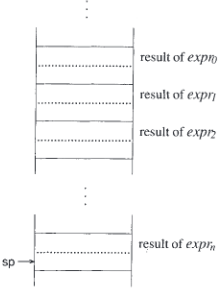
\includegraphics[width=2.19in,height=2.88in]{ib-img/invokestack.png}
\end{center}

The meaning of the expression, and hence the action taken by
\texttt{invoke}, depends on the result produced by
\textit{expr\TextSubscript{0}}. If the value of
\textit{expr\TextSubscript{0}} is an integer or convertible to an
integer, the invocation expression corresponds to mutual
evaluation. If this integer is negative, it is converted to the
corresponding positive value with respect to the number of arguments,
If the value is between one and n, the corresponding descriptor is
copied on top of the result of \textit{expr\TextSubscript{0}},
\texttt{sp} is set to this position, and \texttt{invoke} transfers
control to the beginning of the interpretive loop. On the other hand,
if the value is out of range, \texttt{invoke} fails. Note that the
returned value overwrites the descriptor for
\textit{expr\TextSubscript{0}}, whereas for operators a null-valued
descriptor is pushed to receive the value.

If the value of \textit{expr\TextSubscript{0}} is a function or a
procedure, the corresponding function or procedure must be invoked
with the appropriate arguments. A function or procedure value is
represented by a descriptor that points to a block that contains
information about the function or procedure.

\section[10.2 Procedure Blocks]{10.2 Procedure Blocks}

Functions and procedures have similar blocks, and there is no
source-language type distinction between them.

\textbf{Blocks for Procedures. }Blocks for procedures are constructed
by the linker, using information provided by the translator. Such
blocks are read in as part of the icode file when an Icon program is
executed. The block for a procedure contains the usual title and size
words, followed by six words that characterize the procedure:

\liststyleLxi
\begin{enumerate}
\item 
The icode location of the first virtual machine instruction for the procedure.
\item 
\ The number of arguments expected by the procedure.
\item 
\ The number of local identifiers in the procedure.
\item 
\ The number of static identifiers in the procedure.
\item 
The index in the static identifier array of the first
static identifier in the procedure.
\item 
A C string for the name of the file in which the procedure
declaration occurred.
\end{enumerate}

The remainder of the procedure block contains qualifiers: one for the
string name of the procedure, then others for the string names of the
arguments, local identifiers, and static identifiers, in that order.


For example, the procedure declaration

{\ttfamily\mdseries
\ \ \ procedure calc(i,j)}

{\ttfamily\mdseries
\ \ \ local k}

{\ttfamily\mdseries
\ \ \ static base, index}

{\ttfamily\mdseries
\ \ \ \ \ \ \ \ \ \ \ .}

{\ttfamily\mdseries
\ \ \ \ \ \ \ \ \ \ \ .}

{\ttfamily\mdseries
\ \ \ \ \ \ \ \ \ \ \ .}

{\ttfamily\mdseries
\ \ \ end}


\noindent has the following procedure block:


\ \  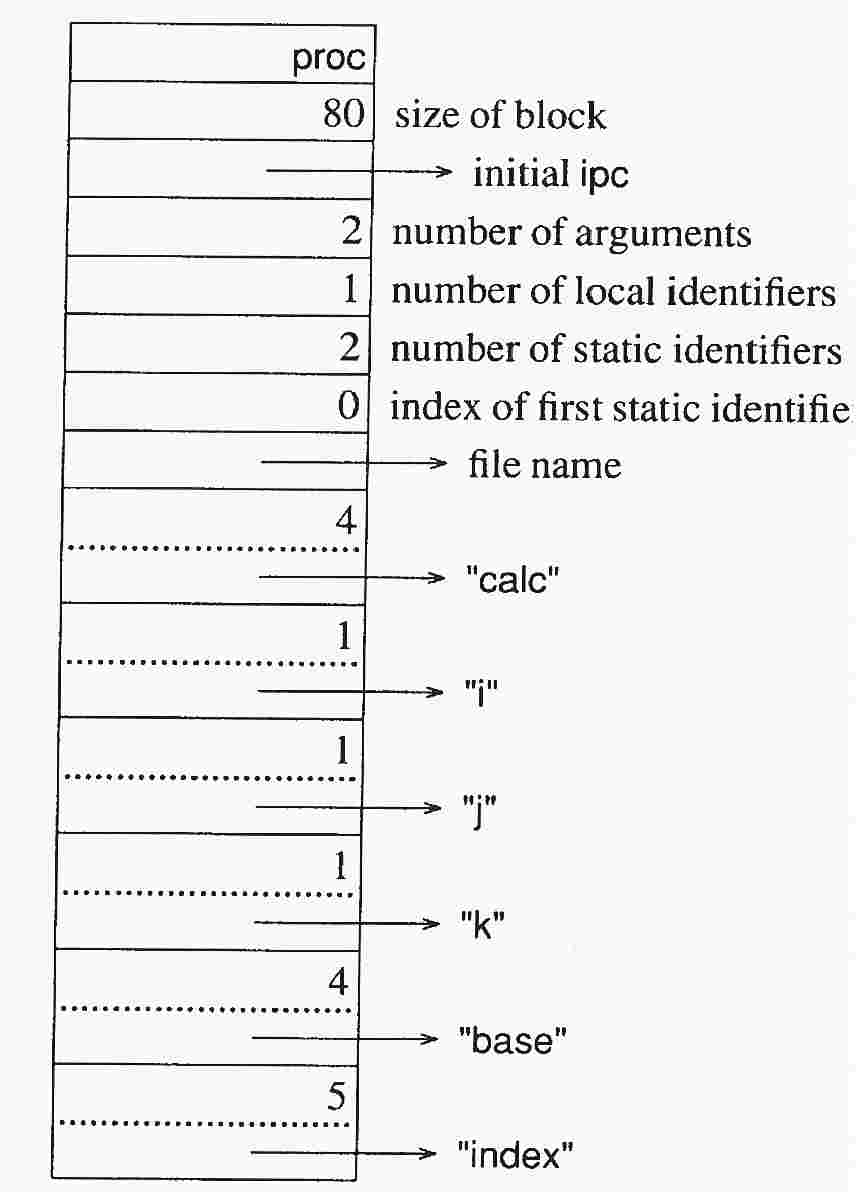
\includegraphics[width=2.8846in,height=3.9807in]{ib-img/ib-img077.jpg} 


The 0 value for the index in the static identifier array indicates
that base is the first static identifier in the program. The indices
of static identifiers are zero-based and increase throughout a program
as static declarations occur.


\textbf{Blocks for Functions.} Blocks for functions are created by the
macro FncDcl that occurs at the beginning of every C function that
implements an Icon function. Such blocks for functions are similar to
those for procedures but are distinguished by the value -1 in the word
that otherwise contains the number of local identifiers. The entry
point is the entry point of the C routine for the function. The
procedure block for \texttt{repl} is typical:


\ \  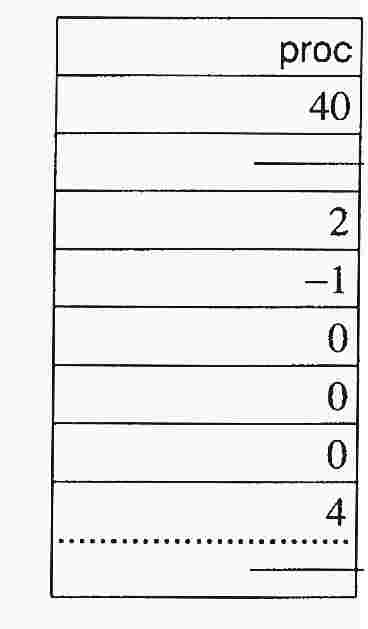
\includegraphics[width=1.2819in,height=2.1008in]{ib-img/ib-img078.jpg} 

\begin{center}
\begin{minipage}{1.948in}

size of block


{}-{\textgreater} C entry point number of arguments function indicator


not used


not used


not used


\bigskip


\bigskip


{}-{\textgreater} {\textquotedbl}repl{\textquotedbl}
\end{minipage}
\end{center}

Note that there are no argument names.


Some functions, such as \texttt{write()}, allow an arbitrary number of
arguments. This is indicated by the value -1 in place of the number of
arguments:


\ \  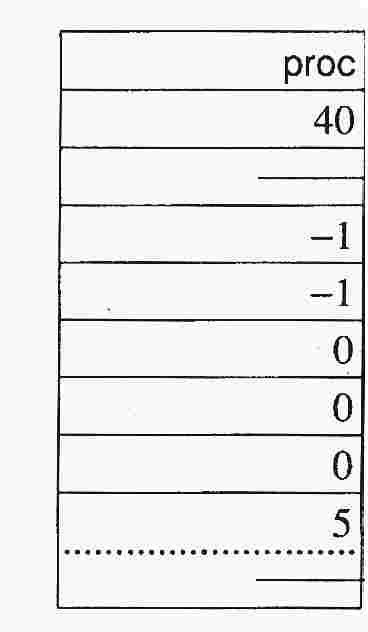
\includegraphics[width=1.2819in,height=2.1098in]{ib-img/ib-img079.jpg} 

\begin{center}
\begin{minipage}{3.0154in}

size of block


{}-{\textgreater} C entry point\newline
indicator of a variable number of arguments\newline
function indicator


not used


not used


not used


\bigskip


{}-{\textgreater} {\textquotedbl}write{\textquotedbl}
\end{minipage}
\end{center}


\section[10.3 Invocation]{10.3 Invocation}
\subsection[10.3.1 Argument Processing]{10.3.1 Argument Processing}

Argument processing begins by dereferencing the arguments in place on
the stack. If a fixed number of arguments is specified in the
procedure block, this number is compared with the argument of
\texttt{invoke}, which is the number of arguments on the stack.


If there are too many arguments, \texttt{sp} is set to point to the
last one expected. For example, the expression

{\ttfamily\mdseries
\ \ numeric(i, j)}

\noindent results in

\bigskip

\ \  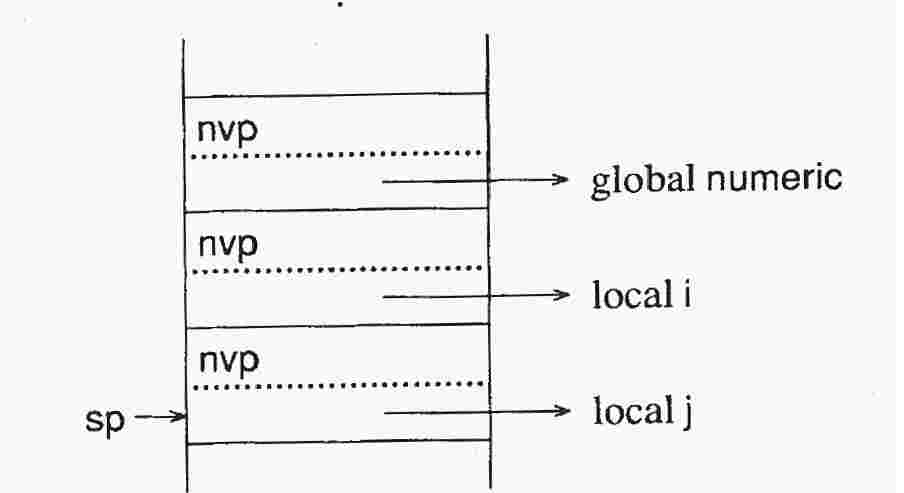
\includegraphics[width=3.0984in,height=1.6457in]{ib-img/ib-img080.jpg} 


Since \texttt{numeric()} expects only one argument, \texttt{sp} is reset, effectively popping the second argument:\ \ 
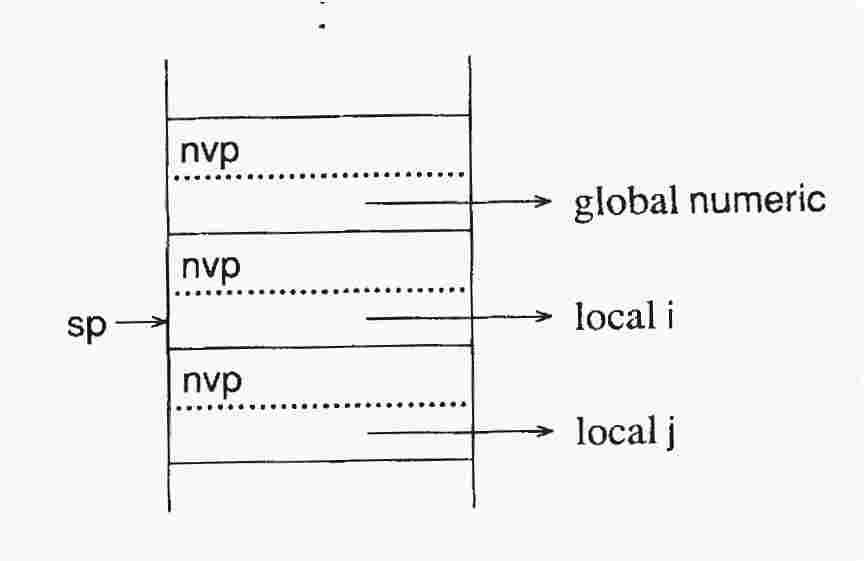
\includegraphics[width=2.8846in,height=1.8728in]{ib-img/ib-img081.jpg} 

On the other hand, if there are not enough arguments, null-valued
descriptors pushed to supply the missing arguments.  For example, the
expression

{\ttfamily\mdseries
\ \ left(s, i)}

\noindent results in

\ \  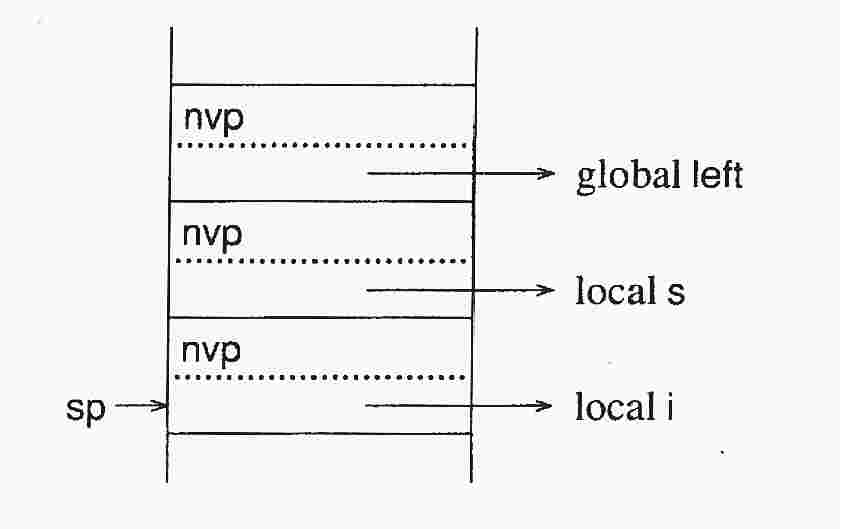
\includegraphics[width=2.8846in,height=1.7661in]{ib-img/ib-img082.jpg} 

and a null value is pushed to provide the missing third argument:

\ \  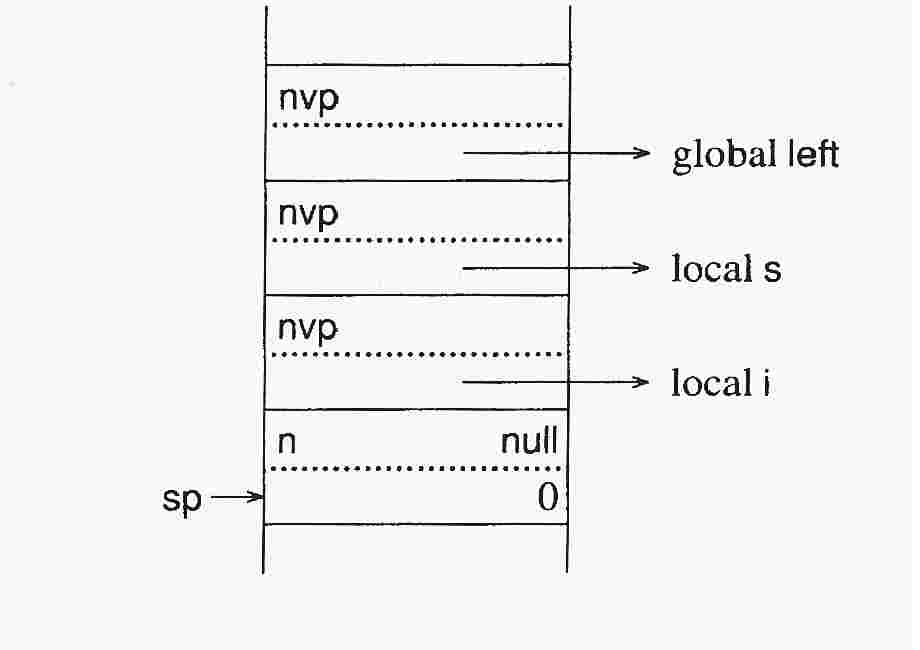
\includegraphics[width=3.0984in,height=2.1701in]{ib-img/ib-img083.jpg} 

\subsection[10.3.2 Function Invocation]{10.3.2 Function Invocation}

Function invocation involves calling a C function in a fashion that is
very similar to evaluating an operator. In the case of an Icon
function, the entry point of the corresponding C function is obtained
from the procedure block rather than by indexing an array of function
pointers corresponding to operator codes.

For an Icon function that has a fixed number of arguments, the C
function is called with a single argument that is a pointer to the
location of Arg0 on the interpreter stack. Note that Arg0 is the
descriptor that points to the procedure block. For an Icon function
that may be called with an arbitrary number of arguments, the C
function is called with two arguments: the number of arguments on the
stack and a pointer to Arg0.

Like an operator, a function may fail, return a result, or
suspend. The coding protocol is the same as for operators.  The
function find is an example:

{\ttfamily\mdseries
function\{*\} find(s1,s2,i,j)}

{\ttfamily\mdseries
\ \ \ str\_anal( s2, i, j )}

{\ttfamily\mdseries
\ \ \ if !cnv:string(s1) then}

{\ttfamily\mdseries
\ \ \ \ \ \ runerr(103,s1)}

{\ttfamily\mdseries
\ \ \ body \{}

{\ttfamily\mdseries
\ \ \ \ \ \ register char *str1, *str2;}

{\ttfamily\mdseries
\ \ \ \ \ \ C\_integer s1\_len, l, term;}


\bigskip

{\ttfamily\mdseries
\ \ \ \ \ \ /*}

{\ttfamily\mdseries
\ \ \ \ \ \ \ * Loop through s2[i:j] trying to find s1 at each point,}

{\ttfamily\mdseries
\ \ \ \ \ \ \ * stopping when the remaining portion s2[i:j] is too short}

{\ttfamily\mdseries
\ \ \ \ \ \ \ * to contain s1. Optimize me!}

{\ttfamily\mdseries
\ \ \ \ \ \ \ */}

{\ttfamily\mdseries
\ \ \ \ \ \ s1\_len = StrLen(s1);}

{\ttfamily\mdseries
\ \ \ \ \ \ term = cnv\_j - s1\_len;}

{\ttfamily\mdseries
\ \ \ \ \ \ while (cnv\_i {\textless}= term) \{}

{\ttfamily\mdseries
\ \ \ \ \ \ \ \ \ str1 = StrLoc(s1);}

{\ttfamily\mdseries
\ \ \ \ \ \ \ \ \ str2 = StrLoc(s2) + cnv\_i - 1;}

{\ttfamily\mdseries
\ \ \ \ \ \ \ \ \ l \ \ \ = s1\_len;}


\bigskip

{\ttfamily\mdseries
\ \ \ \ \ \ \ \ \ /*}

{\ttfamily\mdseries
\ \ \ \ \ \ \ \ \ \ * Compare strings on a byte-wise basis; if the end is}

{\ttfamily\mdseries
\ \ \ \ \ \ \ \ \ \ * reached before inequality is found, suspend with the}

{\ttfamily\mdseries
\ \ \ \ \ \ \ \ \ \ * position of the string.}

{\ttfamily\mdseries
\ \ \ \ \ \ \ \ \ \ */}

{\ttfamily\mdseries
\ \ \ \ \ \ \ \ \ do \{}

{\ttfamily\mdseries
\ \ \ \ \ \ \ \ \ \ \ \ if (l-{}- {\textless}= 0) \{}

{\ttfamily\mdseries
\ \ \ \ \ \ \ \ \ \ \ \ \ \ \ suspend C\_integer cnv\_i;}

{\ttfamily\mdseries
\ \ \ \ \ \ \ \ \ \ \ \ \ \ \ break;}

{\ttfamily\mdseries
\ \ \ \ \ \ \ \ \ \ \ \ \ \ \ \}}

{\ttfamily\mdseries
\ \ \ \ \ \ \ \ \ \ \ \ \} while (*str1++ == *str2++);}

{\ttfamily\mdseries
\ \ \ \ \ \ \ \ \ cnv\_i++;}

{\ttfamily\mdseries
\ \ \ \ \ \ \ \ \ \}}

{\ttfamily\mdseries
\ \ \ \ \ \ fail;}

{\ttfamily\mdseries
\ \ \ \ \ \ \}}

{\ttfamily\mdseries
end}

\texttt{str\_anal()} is an RTL multi-line macro for performing the
standard conversions and defaulting for string analysis functions. It
takes as arguments the parameters for subject, beginning position, and
ending position. It produces declarations for these 3 names prepended
with \texttt{cnv\_}. These variables will contain the converted
versions of the arguments.

{\ttfamily\mdseries
\#begdef str\_anal(s, i, j)}

{\ttfamily\mdseries
\ \ \ declare \{}

{\ttfamily\mdseries
\ \ \ \ \ \ C\_integer cnv\_ \#\# i;}

{\ttfamily\mdseries
\ \ \ \ \ \ C\_integer cnv\_ \#\# j;}

{\ttfamily\mdseries
\ \ \ \ \ \ \}}


\bigskip

{\ttfamily\mdseries
\ \ \ abstract \{}

{\ttfamily\mdseries
\ \ \ \ \ \ return integer}

{\ttfamily\mdseries
\ \ \ \ \ \ \}}


\bigskip

{\ttfamily\mdseries
\ \ \ if is:null(s) then \{}

{\ttfamily\mdseries
\ \ \ \ \ \ inline \{}

{\ttfamily\mdseries
\ \ \ \ \ \ \ \ \ s = k\_subject;}

{\ttfamily\mdseries
\ \ \ \ \ \ \ \ \ \}}

{\ttfamily\mdseries
\ \ \ \ \ \ if is:null(i) then inline \{}

{\ttfamily\mdseries
\ \ \ \ \ \ \ \ \ cnv\_ \#\# i = k\_pos;}

{\ttfamily\mdseries
\ \ \ \ \ \ \ \ \ \}}

{\ttfamily\mdseries
\ \ \ \ \ \ \}}

{\ttfamily\mdseries
\ \ \ else \{}

{\ttfamily\mdseries
\ \ \ \ \ \ if !cnv:string(s) then}

{\ttfamily\mdseries
\ \ \ \ \ \ \ \ \ runerr(103,s)}

{\ttfamily\mdseries
\ \ \ \ \ \ if is:null(i) then inline \{}

{\ttfamily\mdseries
\ \ \ \ \ \ \ \ \ cnv\_ \#\# i = 1;}

{\ttfamily\mdseries
\ \ \ \ \ \ \ \ \ \}}

{\ttfamily\mdseries
\ \ \ \ \ \ \}}


\bigskip

{\ttfamily\mdseries
\ \ \ if !is:null(i) then}

{\ttfamily\mdseries
\ \ \ \ \ \ if cnv:C\_integer(i,cnv\_ \#\# i) then inline \{}

{\ttfamily\mdseries
\ \ \ \ \ \ \ \ \ if ((cnv\_ \#\# i = cvpos(cnv\_ \#\# i, StrLen(s))) ==}

{\ttfamily\mdseries
\ \ \ \ \ \ \ \ \ \ \ \ \ \ CvtFail)}

{\ttfamily\mdseries
\ \ \ \ \ \ \ \ \ \ \ \ fail;}

{\ttfamily\mdseries
\ \ \ \ \ \ \ \ \ \}}

{\ttfamily\mdseries
\ \ \ \ \ \ else}

{\ttfamily\mdseries
\ \ \ \ \ \ \ \ \ runerr(101,i)}


\bigskip

{\ttfamily\mdseries
\ \ \ \ if is:null(j) then inline \{}

{\ttfamily\mdseries
\ \ \ \ \ \ \ cnv\_ \#\# j = StrLen(s) + 1;}

{\ttfamily\mdseries
\ \ \ \ \ \ \ \}}

{\ttfamily\mdseries
\ \ \ \ else if cnv:C\_integer(j,cnv\_ \#\# j) then inline \{}

{\ttfamily\mdseries
\ \ \ \ \ \ \ if ((cnv\_ \#\# j = cvpos(cnv\_ \#\# j, StrLen(s))) == CvtFail)}

{\ttfamily\mdseries
\ \ \ \ \ \ \ \ \ \ fail;}

{\ttfamily\mdseries
\ \ \ \ \ \ \ if (cnv\_ \#\# i {\textgreater} cnv\_ \#\# j) \{}

{\ttfamily\mdseries
\ \ \ \ \ \ \ \ \ \ register C\_integer tmp;}

{\ttfamily\mdseries
\ \ \ \ \ \ \ \ \ \ tmp = cnv\_ \#\# i;}

{\ttfamily\mdseries
\ \ \ \ \ \ \ \ \ \ cnv\_ \#\# i = cnv\_ \#\# j;}

{\ttfamily\mdseries
\ \ \ \ \ \ \ \ \ \ cnv\_ \#\# j = tmp;}

{\ttfamily\mdseries
\ \ \ \ \ \ \ \ \ \ \}}

{\ttfamily\mdseries
\ \ \ \ \ \ \ \}}

{\ttfamily\mdseries
\ \ \ \ else}

{\ttfamily\mdseries
\ \ \ \ \ \ \ runerr(101,j)}

{\ttfamily\mdseries
\#enddef}

\subsection[10.3.3 Procedure Invocation]{10.3.3 Procedure Invocation}

In the case of procedure invocation, a \textit{procedure frame} is
pushed onto the interpreter stack to preserve information that may be
changed during the execution of the procedure and that must be
restored when the procedure returns. As for other types of frames, a
procedure frame begins with a marker. A procedure frame marker
consists of eight words:


\ \  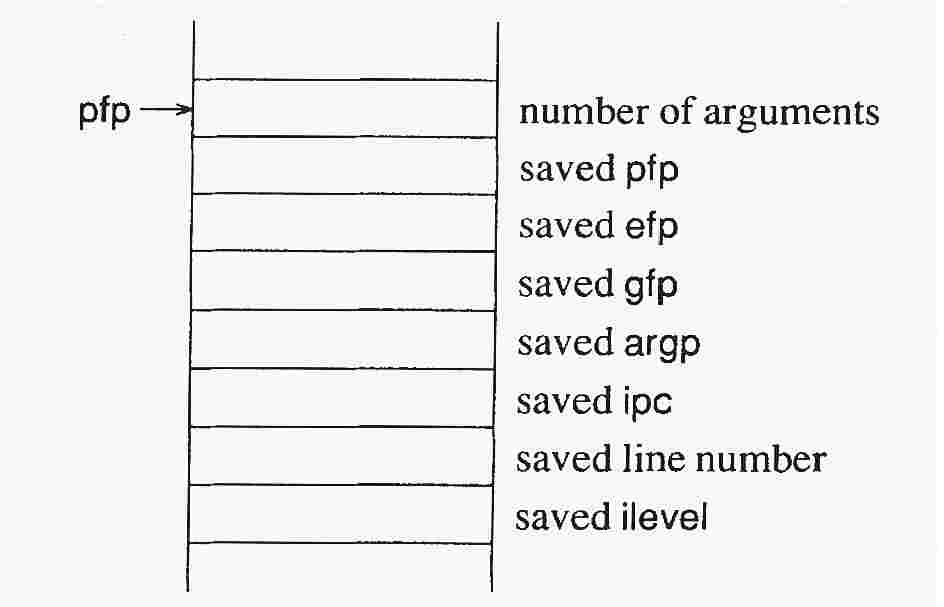
\includegraphics[width=3.2063in,height=2.0272in]{ib-img/ib-img084.jpg} 


The current procedure frame is pointed to by \texttt{pfp}, and
\texttt{argp} points to the place on the interpreter stack where the
arguments begin, analogous to Arg0 for functions. The number of
arguments, which can be computed from \texttt{pfp} and \texttt{argp},
is provided to make computations related to arguments more convenient.

After the procedure marker is constructed, a null-valued descriptor is
pushed for each local identifier. For example, the call

{\ttfamily\mdseries
\ \ calc(3,4)}

\noindent for the procedure declaration given in Sec. 10.2 produces


\ \  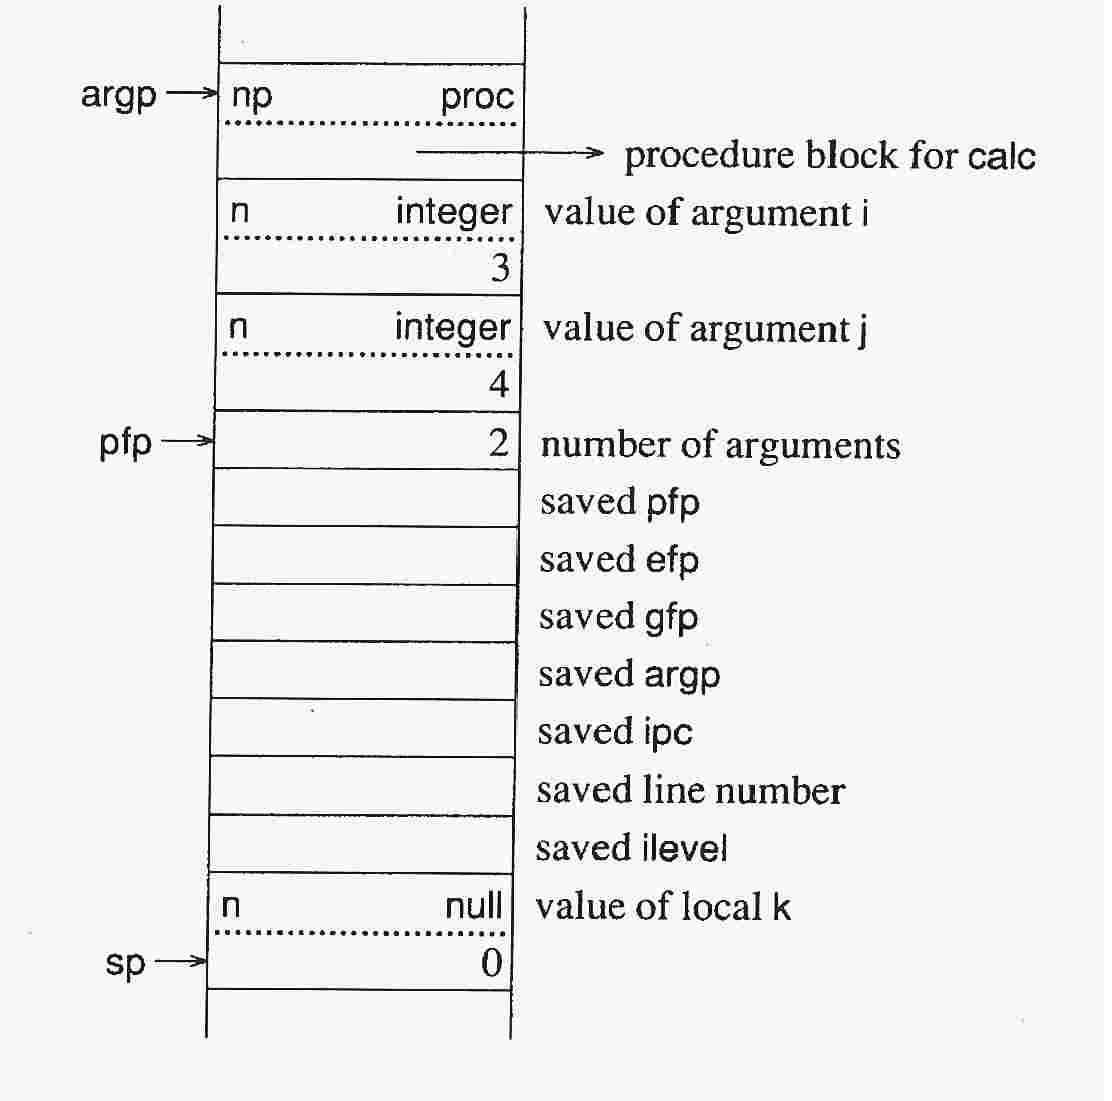
\includegraphics[width=3.7402in,height=3.6772in]{ib-img/ib-img085.jpg} 


Once the null values for the local identifiers are pushed,
\texttt{ipc} is set to the entry point given in the procedure block
and \texttt{efp} and \texttt{gfp} are set to zero. Execution then
continues in the interpreter with the new \texttt{ipc}.

The three forms of return from a procedure are the same as those from
a function and correspond to the source-language expressions

{\ttfamily\mdseries
\ \ \ return e}

{\ttfamily\mdseries
\ \ \ fail}

{\ttfamily\mdseries
\ \ \ suspend e}


The corresponding virtual machine instructions are \texttt{pret},
\texttt{pfail}, and \texttt{psusp}. For example, the virtual machine
code for

{\ttfamily\mdseries
\ \ \ return \&null}

\noindent is

{\ttfamily\mdseries
\ \ \ pnull}

{\ttfamily\mdseries
\ \ \ pret}


In the case of \texttt{pret}, the result currently on the top of the
interpreter stack is copied on top of the descriptor pointed to by
\texttt{argp}. If this result is a variable that is on the stack (and
hence local to the current procedure call), it is dereferenced in
place. The C stack is unwound, since there may be suspended generators
at the time of the return. The values saved in the procedure frame
marker are restored, and execution continues in the interpreter with
the restored \texttt{ipc}.

In the case of failure, the C stack is unwound as it is for
\texttt{pret}, values arc restored from the procedure frame marker,
and control is transferred to \texttt{efail}.

Procedure suspension is similar to other forms of suspension. The
descriptor on the top of the interpreter stack is dereferenced, if
necessary, and saved. A generator frame marker is constructed on the
interpreter stack to preserve values that may be needed if the
procedure call is resumed. For procedure suspension, a generator frame
marker contains two words in addition to those needed for other kinds
of generator frame markers and has the form

\ \  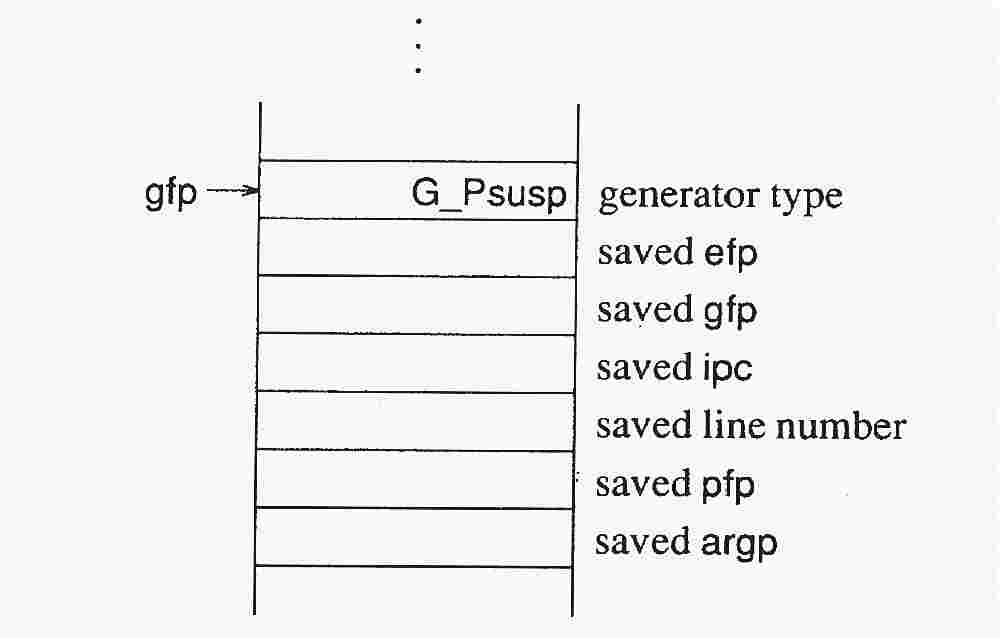
\includegraphics[width=3.6098in,height=2.2835in]{ib-img/ib-img086.jpg} 

After the generator frame marker is pushed, the portion of the stack
between the last generator or expression frame marker before the call
to this procedure and the word prior to \texttt{argp} is copied to the
top of the stack.  Finally, the saved descriptor, which is the result
produced by the procedure, is pushed on the top of the stack.
Execution then continues in the interpreter with the restored
\texttt{ipc}.

\section[10.4 Co{}-Expressions]{10.4 Co-Expressions}

Co-expressions add another dimension to expression evaluation in
Icon. The important thing to understand about co-expressions is that
Icon evaluation is always in \textit{some }co-expression. Although it
is not evident, the execution of an Icon program begins in a
co-expression, namely the value of \texttt{\&main}.

A co-expression requires both an interpreter stack and a C stack. In
the co-expression for \texttt{\&main}, the interpreter stack is
statically allocated and the C stack is the one normally used for C
execution--the {\textquotedbl}system stack{\textquotedbl} on some
computers. The creation of a new co-expression produces a new
interpreter stack and a new C stack, as well as space that is needed
to save state information. When a co-expression is activated, the
context for evaluation is changed to the stacks for the activated
co-expression. When the activation of a co-expression produces a
result, it in turn activates the co-expression that activated it,
leaving the stacks from which the return occurred in a state of
suspension. Thus, co-expression activation constitutes a simple
context switch.  In every co-expression, expression evaluation is in
some state, possibly actively executing, possibly suspended, or
possibly complete and unreachable.


The virtual machine instructions for

{\ttfamily\mdseries
\ \ \ create \textit{expr\TextSubscript{0}}}

are

{\ttfamily\mdseries
\ \ \ \ \ \ goto L3}

{\ttfamily\mdseries
L1:}

{\ttfamily\mdseries
\ \ \ \ \ \ pop}

{\ttfamily\mdseries
\ \ \ \ \ \ mark L2}

{\ttfamily\itshape
\ \ \ \ \ \ code for expr\TextSubscript{0}}

{\ttfamily\mdseries
\textrm{\textit{\ \ \ \ \ \ }}\textrm{coret}}

{\ttfamily\mdseries
\ \ \ \ \ \ efail}

{\ttfamily\mdseries
L2:}

{\ttfamily\mdseries
\ \ \ \ \ \ cofail}

{\ttfamily\mdseries
\ \ \ \ \ \ goto L2}

{\ttfamily\mdseries
L3:}

{\ttfamily\mdseries
\ \ \ \ \ \ create\ \ L1}


Control goes immediately to \texttt{L3}, where the instruction create
constructs a co-expression block and returns a descriptor that points
to it. This block contains space for i-state variables, space for the
state of the C stack, an interpreter stack, and a C stack.

The code between \texttt{L1} and \texttt{L3} is not executed until the
co-expression is activated. The pop instruction following \texttt{L1}
discards the result transmitted to a co-expression on its first
activation, since there is no expression waiting to receive the result
of an initial activation. Next, an expression frame marker is created,
and the code for \textit{expr\TextSubscript{0}} is executed. If
\textit{expr\TextSubscript{0}} produces a result, \texttt{coret} is
executed to return the result to the activating expression. If the
co-expression is activated again, its execution continues with efail,
which causes any suspended generators in the code for
\textit{expr\TextSubscript{0}} to be resumed. If
\textit{expr\TextSubscript{0}} fails, the expression frame is removed
and \texttt{cofail} is executed. The \texttt{cofail} instruction is
very similar to the \texttt{coret} instruction, except that it signals
failure rather than producing a result. Note that if a co-expression
that returns by means of \texttt{cofail} is activated again, the
\texttt{cofail} instruction is executed in a loop.

A co-expression is activated by the expression

{\ttfamily\mdseries
\textit{\ \ \ expr1 }@ \textit{expr2}}

\noindent for which the virtual machine code is

{\itshape
\ \ \ code for expr1}

{\itshape
\ \ \ code for expr2}


\ \ \ coact


The more common form of activation,
\texttt{@}\textit{expr\TextSubscript{0}}, is just an abbreviation for
\texttt{\&null @} \textit{expr\TextSubscript{0}}; a result is always
transmitted, even if it is the null value.

The virtual machine code for \textit{expr\TextSubscript{1}} produces
the descriptor for the result that is to be transmitted to the
co-expression being activated. The \texttt{coact} instruction
dereferences the result produced by \textit{expr\TextSubscript{2}}, if
necessary, and checks to make sure it is a co-expression. After
setting up state information, \texttt{coact} transfers control to the
new co-expression with \texttt{ipc} set to \texttt{L1}. Execution
continues there. If \texttt{coret} is reached, control is restored to
the activating co-expression. The instructions \texttt{coact} and
\texttt{coret} are very similar. Each saves the current co-expression
state, sets up the new co-expression state, and transfers control.

\textbf{Co-Expression Blocks.} There is quite a bit of information
associated with a co-expression, and space is provided for it in a
co-expression block:


\bigskip

\clearpage
\ \  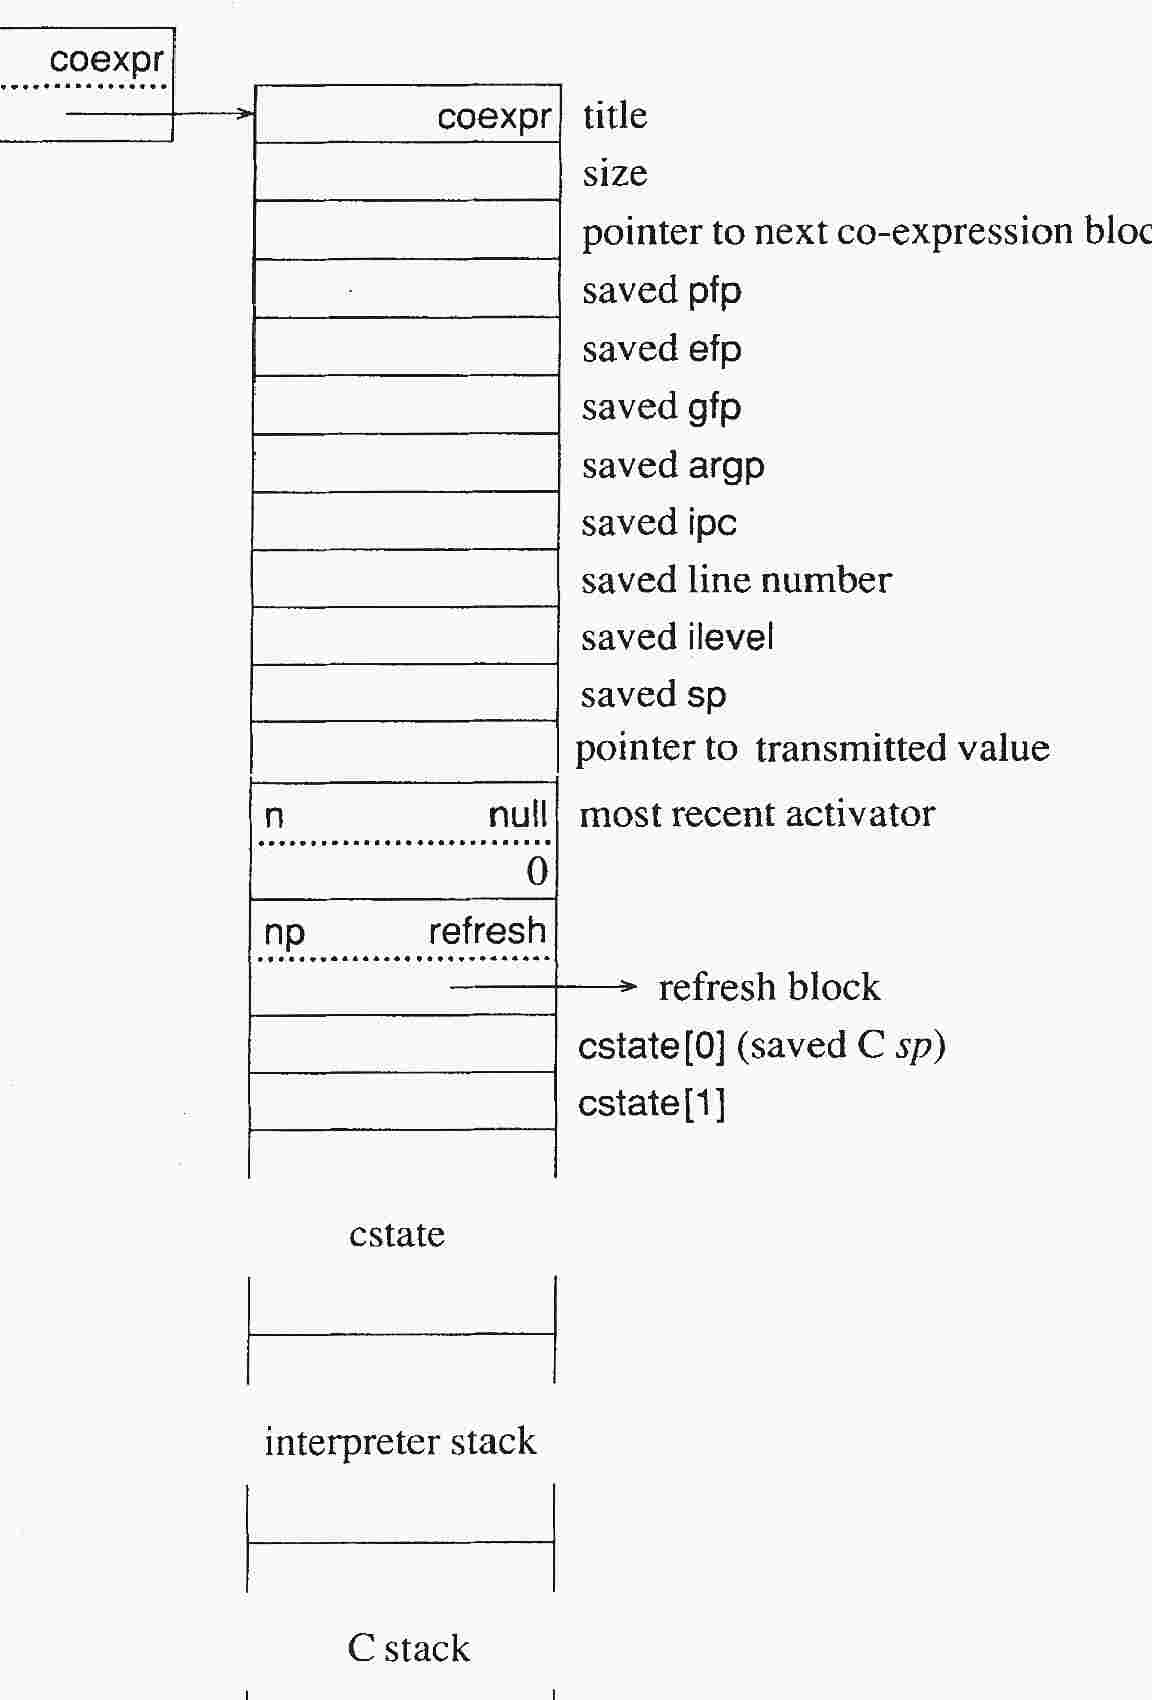
\includegraphics[width=3.9543in,height=5.678in]{ib-img/ib-img087.jpg} 


The interpreter stack and C stack shown in this diagram are not to
scale compared with the rest of the block. Both are comparatively
large; the actual sizes depend on the address space of the target
computer.


The first word of the block is the usual title. The next word contains
the number of results the co-expression has produced-its
{\textquotedbl}size.{\textquotedbl} Then there is a pointer to the
next co-expression block on a list that is maintained for garbage
collection purposes. See Sec. 11.3.4. Following this pointer there are
i-state variables: \texttt{pfp}, \texttt{efp}, \texttt{gfp},
\texttt{argp}, \texttt{ipc}, \texttt{sp}, the current program line
number, and \texttt{ilevel}.

Then there is a descriptor for the transmitted result, followed by two
more descriptors: one for the co-expression that activates this one
and one for a \textit{refresh} block that is needed if a copy of this
co-expression block is needed.  C state information is contained in an
array of words, \texttt{cstate}, for registers and possibly other
state information. The array \texttt{cstate} typically contains
fifteen words for such information. The C \textit{sp} is stored in
\texttt{cstate[0]}. The use of the rest of \texttt{cstate} is
machine-dependent.

Finally, there is an interpreter stack and a C stack. On a computer
with a downward-growing C stack, such as the VAX, the base of the C
stack is at the end of the co-expression block and the interpreter and
C stacks grow toward each other. On a computer with an upward-growing
C stack, the C stack base follows the end of the interpreter stack.

\textbf{Stack Initialization.} When a co-expression is first
activated, its interpreter stack must be in an appropriate state. This
initialization is done when the co-expression block is created. A
procedure frame, which is a copy of the procedure frame for the
procedure in which the create instruction is executed, is placed on
the new stack. It consists of the words from \texttt{argp} through the
procedure frame marker and the descriptors for the local
identifiers. The \texttt{efp} and \texttt{gfp} in the co-expression
block are set to zero and the \texttt{ipc} is set to the value given
in the argument to the \texttt{create} instruction (\texttt{L1}).

No C state is set up on the new C stack; this is handled when the co-expression is activated the first time. The initial
null value for the activator indicates the absence of a valid C state.


\textbf{Co-Expression Activation.} As mentioned previously,
\texttt{coact} and \texttt{coret} perform many similar functions--both
save current state information, establish new state information, and
activate another co-expression.  The current i-state variables are
saved in the current co-expression block, and new ones are established
from the co-expression block for the co-expression being
activated. Similar actions are taken for the C state. Since the C
state is machine-dependent, the {\textquotedbl}context
switch{\textquotedbl} for the C state is performed by a routine,
called \texttt{coswitch()}, that contains assembly-language code.

The C state typically consists of registers that are used to address
the C stack and registers that must be preserved across the call of a
C function. On the VAX, for example, the C stack registers are
\textit{sp, ap, and fp}. Only the registers \texttt{r6} through
\texttt{r11} must be saved for some C compilers, while other C
compilers require that \texttt{r3} through \texttt{r11} be saved. Once
the necessary registers are saved in the \texttt{cstate} array of the
current co-expression, new values of these registers are
established. If the co-expression being activated has been activated
before, the C state is set up from its \texttt{cstate} array, and
\texttt{coswitch()} returns to \texttt{interp()}. At this point,
execution continues in the newly activated co-expression. Control is
transferred to the beginning of the interpreter loop, and the next
instruction (from the \texttt{ipc} for the co-expression) is fetched.

However, when a co-expression is activated for the first time, there
are no register values to restore, since no C function has yet been
called for the new co-expression. This is indicated, as mentioned
previously, by a null activator, which is communicated to
\texttt{coswitch()} by an integer argument. In this case,
\texttt{coswitch()} sets up registers for the call of a C function and
calls \texttt{interp()} to start the execution of the new
co-expression.  Such a call to \texttt{interp()} on the first
activation of a co-expression corresponds to the call to
\texttt{interp()} that starts program execution in the co-expression
\texttt{\&main} for the main procedure. There can never be a return
from the call to \texttt{interp()} made in \texttt{coswitch()}, since
program execution can only terminate normally by a return from the
main procedure, in \texttt{\&main}.

The function \texttt{coswitch()} is fastest if it is
machine-dependent. The version for the x86 with the GCC compiler is an
example:

{\ttfamily\mdseries
coswitch:}

{\ttfamily\mdseries
\ \ pushl \%ebp}

{\ttfamily\mdseries
\ \ movl \%esp,\%ebp}

{\ttfamily\mdseries
\ \ movl 8(\%ebp),\%eax}

{\ttfamily\mdseries
\ \ movl \%esp,0(\%eax)}

{\ttfamily\mdseries
\ \ movl \%ebp,4(\%eax)}

{\ttfamily\mdseries
\ \ movl 12(\%ebp),\%eax}

{\ttfamily\mdseries
\ \ cmpl \$0,16(\%ebp)}

{\ttfamily\mdseries
\ \ movl 0(\%eax),\%esp}

{\ttfamily\mdseries
\ \ je .L2}


\bigskip

{\ttfamily\mdseries
\ \ movl 4(\%eax),\%ebp}

{\ttfamily\mdseries
\ \ jmp .L1}


\bigskip

{\ttfamily\mdseries
.L2:}

{\ttfamily\mdseries
\ \ movl \$0,\%ebp}

{\ttfamily\mdseries
\ \ pushl \$0}

{\ttfamily\mdseries
\ \ pushl \$0}

{\ttfamily\mdseries
\ \ call new\_context}

{\ttfamily\mdseries
\ \ pushl \$.LC0}

{\ttfamily\mdseries
\ \ call syserr}

{\ttfamily\mdseries
\ \ addl \$12,\%esp}


\bigskip

{\ttfamily\mdseries
.L1:}

{\ttfamily\mdseries
\ \ leave}

{\ttfamily\mdseries
\ \ ret}


If no assembler co-expression switch is available, modern platforms
with POSIX threads can use Icon 9.5.1's supported form of
co-expressions, which is more than 100x slower and approximately twice
as many lines of C. The public interface in either case looks like:

{\ttfamily\mdseries
int coswitch(void *old\_cs, void *new\_cs, int first);}

The variables \texttt{old\_cs} and \texttt{new\_cs} are pointers to
the \texttt{cstate} arrays for the activating and activated
co-expressions, respectively. The value of first is 0 if the
co-expression is being activated for the first time. Note that in
order to write \texttt{coswitch()} it is necessary to know how the
first two arguments are accessed in assembly language. For the
previous example, \texttt{old\_cs} and \texttt{new\_cs} are eight and
twelve bytes from the \textit{ebp }register, respectively.

\textbf{Refreshing a Co-Expression}. The operation
\texttt{\textit{\^{}}}\textit{expr\TextSubscript{0}} creates a copy of
the co-expression produced by \textit{expr\TextSubscript{0}} with its
state initialized to what it was when it was originally created. The
refresh block for \textit{expr\TextSubscript{0}} contains the
information necessary to reproduce the initial state. The refresh
block contains the original \texttt{ipc} for the co-expression, the
number of local identifiers for the procedure in which
\textit{expr\TextSubscript{0}} was created, a copy of the procedure
frame marker at the time of creation, and the values of the arguments
and local identifiers at the time of creation. Consider, for example,

{\ttfamily\mdseries
\ \ \ procedure labgen(s)}

{\ttfamily\mdseries
\ \ \ \ \ \ local i, j, e}

{\ttfamily\mdseries
\ \ \ \ \ \ i := 1}

{\ttfamily\mdseries
\ \ \ \ \ \ j := 100}

{\ttfamily\mdseries
\ \ \ \ \ \ e := create (s {\textbar}{\textbar} (i to j) {\textbar}{\textbar} {\textquotedbl}:{\textquotedbl})}

{\ttfamily\mdseries
\ \ \ end}


For the call \texttt{labgen({\textquotedbl}L{\textquotedbl})}, the refresh block for \texttt{e} is


\ \  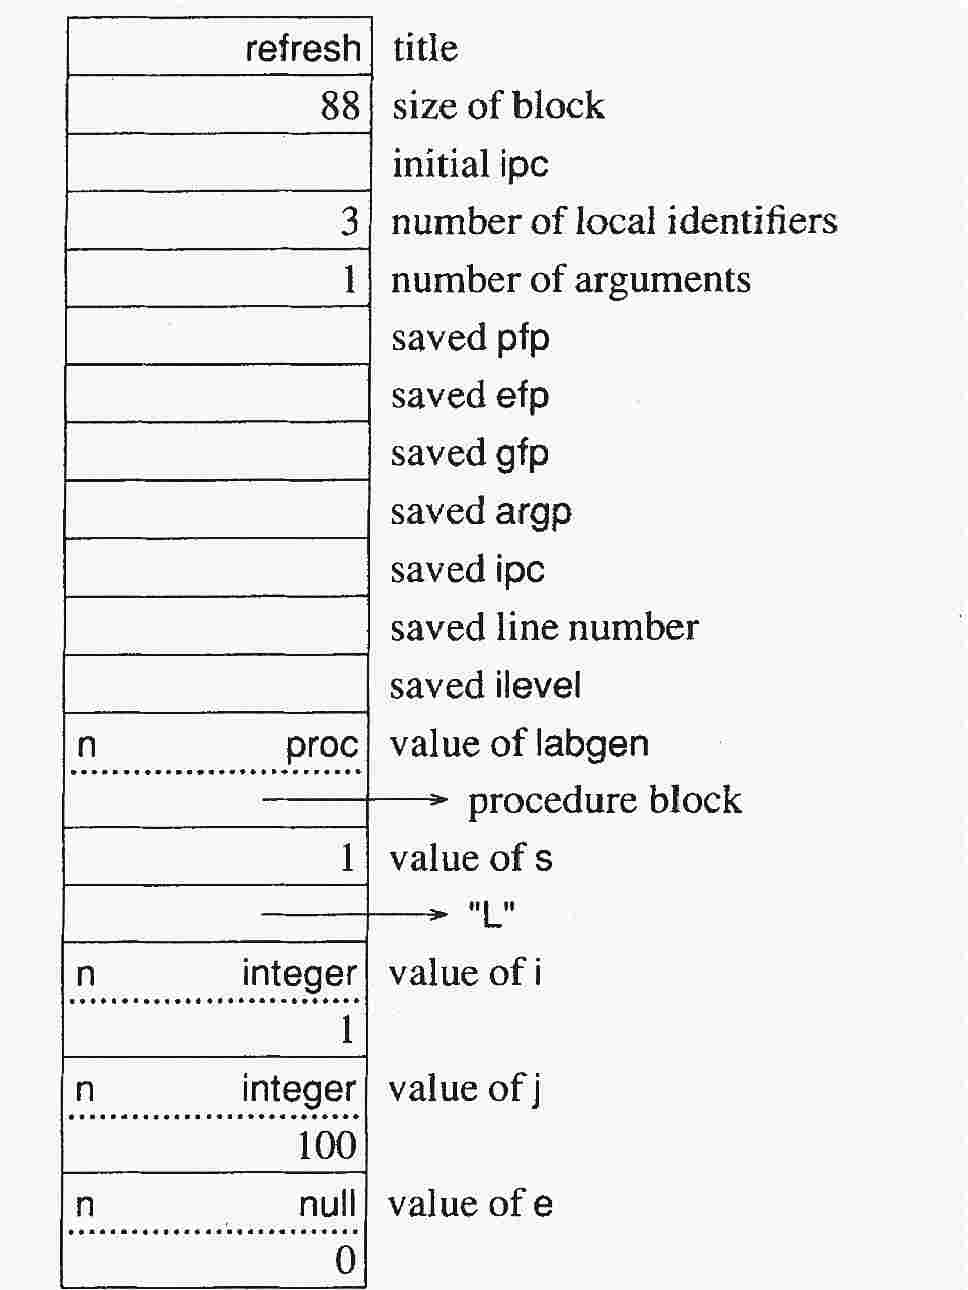
\includegraphics[width=3.3134in,height=4.3075in]{ib-img/ib-img088.jpg} 


\textsc{Retrospective}: Invocation expressions are more complicated to
implement than operators, since the meaning of an invocation
expression is not known until it is evaluated. Since functions and
procedures are source-language values, the information associated with
them is stored in blocks in the same manner as for other types.

The C code that implements Icon functions is written in the same
fashion as the code for operators. Procedures have source-language
analogs of the failure and suspension mechanisms used for implementing
functions and operators.  Procedure frames identify the portions of
the interpreter stack associated with the procedures currently
invoked.

A co-expression allows an expression to be evaluated outside its
lexical site in the program by providing separate stacks for its
evaluation. The possibility of multiple stacks in various states of
evaluation introduces technical problems in the implementation,
including a machine-dependent context switch.

\subsection{EXERCISES}

\textbf{10.1} What happens if a call of a procedure or function
contains an extra argument expression, but the evaluation of that
expression fails?

\textbf{10.2} Sometimes it is useful to be able to specify a function
or procedure by means of its string name. Icon supports
{\textquotedbl}string invocation,{\textquotedbl} which allows the
value of \textit{expr\TextSubscript{0}} in

{\ttfamily\mdseries
\textit{\ \ \ expr\TextSubscript{0}(expr\TextSubscript{1},
expr\TextSubscript{2}, ..., expr\TextSubscript{n})}\ \ .}

\noindent to be a string. Thus,

{\ttfamily\mdseries
\ \ \ {\textquotedbl}write{\textquotedbl}(s)}

\noindent produces the same result as

{\ttfamily\mdseries
\ \ \ write(s)}

Of course, such a string name is usually computed, as in

{\ttfamily\mdseries
\ \ \ (read())(s)}

Describe what is involved in implementing this aspect of
invocation. Operators also may be invoked by their string names, as in

{\ttfamily\mdseries
\ \ \ {\textquotedbl}+{\textquotedbl}(i,j)}

What is needed in the implementation to support this facility? Can a
control structure be invoked by a string name?

\textbf{10.3} If the result returned by a procedure is a variable, it
may need to be dereferenced. This is done in the code for
\texttt{pret} and \texttt{psusp}. For example, if the result being
returned is a local identifier, it must be replaced by its value What
other kinds of variables must be dereferenced? Is there any difference
in the dereferencing done by \texttt{pret} and \texttt{psusp}?

\textbf{10.4} How is the structure of a co-expression block different
on a computer with an upward-growing C stack compared to one with a
downward-growing C stack? What is the difference between the two cases
in terms of potential storage fragmentation?

\chapter{Storage Management}

\begin{quote}
Editorial Note: the implementation of storage management has transformed
over time as computer hardware capabilities have changed. Despite this,
the main principles of Icon and Unicon's garbage collector are
unmodified after several decades.
\end{quote}

\textsc{Perspective}: The implementation of storage management must
accommodate a wide range of allocation requirements.  At the same
time, the implementation must provide generality and some compromise
between ``normal'' programs and those that have unusual
requirements. Although it is clearly sensible to satisfy the needs of
most programs in an efficient manner, there is no way to define what
is typical or to predict how programming style and applications may
change. Indeed, the performance of the implementation may affect both
programming style and applications.

Strings and blocks can be created during program execution at times
that cannot be predicted, in general, from examination of the text of
a program. The sizes of strings and of some types of blocks may vary
and may be arbitrarily large, although practical considerations
dictate some limits. There may be an arbitrary number of strings and
blocks.  The ``lifetimes'' during which they may be used are arbitrary
and are unrelated, in general, to procedure calls and returns.

Different programs vary considerably in the number, type, and sizes of
data objects that are created at run time. Some programs read in
strings, transform them, and write them out without ever creating
other types of objects. Other programs create and manipulate many
lists, sets, and tables but use few strings. Relatively few programs
use co-expressions, but there are applications in which large numbers
of co-expressions are created.

Since a program can construct an arbitrary number of data objects of
arbitrary sizes and lifetimes, some mechanism is needed to allow the
reuse of space for ``dead'' objects that are
no longer accessible to the program. Thus, in addition to a mechanism
for allocating storage for objects at run time, there must be a
storage-reclamation mechanism, which usually is called \textit{garbage
collection}. The methods used for allocation and garbage collection
are interdependent. Simple and fast allocation methods usually require
complex and time-consuming garbage-collection techniques, while more
efficient garbage-collection techniques generally lead to more complex
allocation techniques.

Storage management has influences that are far-reaching. In some
programs, it may account for a major portion of execution time. The
design of data structures, the layout of blocks, and the
representation of strings are all influenced by storage-management
considerations. For example, both a descriptor that points to a block
and the first word of the block contain the same type code. This
information is redundant as far as program execution is concerned,
since blocks are accessed only via descriptors that point to them. The
redundant type information is motivated by storage-management
considerations. During garbage collection, it is necessary to access
blocks directly, rather than through pointers from descriptors, and it
must be possible to determine the type of a block from the block
itself.  Similarly, the size of a block is of no interest in
performing language operations, but the size is needed during garbage
collection. Blocks, therefore, carry some ``overhead'' for storage
management. This overhead consists primarily of extra space,
reflecting the fact that it takes more space to manage storage
dynamically than would be needed if space were allocated
statically. Balancing space overhead against efficiency in allocating
and collecting objects is a complex task.

Such problems have plagued and intrigued implementors since the early
days of LISP. Many ways have been devised to handle dynamic storage
management, and some techniques have been highly refined to meet
specific requirements (Cohen 1981). In the case of Icon, there is
\textit{more }emphasis on storage management for strings than there is
in a language, such as LISP, where lists predominate. Icon's
storage-management system reflects previous experience with
storage-management systems used in XPL (McKeeman, Horning, and Wortman
1970), SNOBOL4 (Hanson 1977), and the earlier Ratfor implementation of
Icon (Hanson 1980). The result is, of course, somewhat idiosyncratic,
but it provides an interesting case study of a real storage-management
system.

%\pagebreak[4]
\noindent\textbf{A brief history of Icon's storage management}\\
%\nopagebreak[4]
The main changes in the overall approach to storage management since
version 6 have been in the treatment of the Allocated Storage areas,
which is discussed in section 11.1 below. Since different programs
have different memory usage patterns, the main issues have always
been: how much memory to set aside, and when, for the different uses
of allocated memory.

\noindent
\begin{xtabular}{l@{\hspace{1cm}}p{13cm}}
Icon V6 & Originally, Icon expected to control all memory itself.
	  Allocated storage was a single contiguous memory extent. On
	  some systems, it could be expanded using the UNIX
	  \texttt{sbrk()} system call.\\
Icon V7 & In order to port Icon widely, an alternative that did not
	  depend on \texttt{sbrk()} was developed in which
          the allocated storage was split into three fixed size
          extents (static, string and block).\\
Icon V8 & The Icon compiler iconc introduced improvements to storage handling.
	  Internally, pointers replace many descriptors in blocks, saving space.
	  The process of registering tended variables with the garbage
	  collector becomes organized and gains syntactic support via RTL.
	  For the sake of systems like MS-DOS, which had 64K
	  allocation limits, multiple string or block storage regions
          are allocated if garbage collection fails to provide enough
          free space to satisfy an allocation request. Storage regions
          that are full may subsequently have space freed and be reused.
\\
Icon V9 & By this point, \texttt{sbrk()} is abandoned and multiple,
	  fixed regions are standard. \\
{\color{blue}Unicon}
        & {\color{blue}
          Each thread uses its own string and block storage regions
          for allocation. A thread that performs garbage collection
          must first suspend every other thread before proceeding.}\\
\end{xtabular}

\section{Memory Layout}

During the execution of an Icon program, memory is logically divided
into several areas based on how the memory is used. The word
``region'' may generically refer to the different sections in the
diagram; in the implementation, it is used more specifically to refer
to individually-allocated chunks of memory within the allocated
storage area.

The sizes and locations of memory regions are dependent on computer
architecture and the operating system used, but typically they have
the following form:
\begin{center}
\begin{picture}(300,200)
%\put(0,0){\graphpaper{30}{20}}
\put(60,160){\framebox(180,40){\sffamily\bfseries run-time system}}
\put(60,120){\framebox(180,40){\sffamily\bfseries icode}}
\put(60,80){\framebox(180,40){\sffamily\bfseries allocated storage}}
\put(60,40){\framebox(180,40){\sffamily\bfseries free space}}
\put(60,0){\framebox(180,40){\sffamily\bfseries system stack}}
\end{picture}
\end{center}

This diagram is not drawn to scale; some regions are much larger than
others.  It is also an abstraction; the regions might or might not be
contiguous, and each is allocated seperately. The free space is
managed by the underlying operating system rather than by the Icon runtime.


\textbf{The Run-Time System}. The run-time system contains the
executable code for the interpreter, built-in operators and functions,
support routines, and so forth. It also contains static storage for
some Icon strings and blocks that appear in C functions.
For example, runtime/data.r contains statically-allocated blocks for
many runtime system entities such as built-in csets.
Such blocks never move, but in some cases their contents may change.
{\color{blue}In Unicon, most non-constant data that was global in Icon
has been moved into a per-program or per-thread structure.}
The size of the run-time system is machine-dependent.

\textbf{The Icode Region}. One of the first things done by the
run-time system is to read in the icode file for the program that is
to be executed. The data in the icode region, which is produced by the
linker, is divided into a number of sections:

\begin{center}
\begin{picture}(300,240)
%\put(0,0){\graphpaper{30}{24}}
\put(60,200){\framebox(180,40){\sffamily\bfseries code and blocks}}
\put(60,160){\framebox(180,40){\sffamily\bfseries record information}}
\put(60,120){\framebox(180,40){\sffamily\bfseries global identifier values}}
\put(60,80){\framebox(180,40){\sffamily\bfseries global identifier names}}
\put(60,40){\framebox(180,40){\sffamily\bfseries static identifier values}}
\put(60,0){\framebox(180,40){\sffamily\bfseries strings}}
\end{picture}
\end{center}

The first section contains virtual machine code, blocks for cset and
real literals, and procedure blocks, on a per-procedure basis. Thus,
the section of the icode region that contains code and blocks consists
of segments of the following form for each procedure:
\begin{center}
\begin{picture}(300,160)
%\put(0,0){\graphpaper{30}{16}}
\put(60,120){\framebox(180,40){\sffamily\bfseries blocks for real literals}}
\put(60,80){\framebox(180,40){\sffamily\bfseries blocks for cset literals}}
\put(60,40){\framebox(180,40){\sffamily\bfseries procedure blocks}}
\put(60,0){\framebox(180,40){\sffamily\bfseries virtual machine instructions}}
\end{picture}
\end{center}

Record information for the entire program is in the second section of
the icode region. Next, there is an array of descriptors for the
values of the global identifiers in the program, followed by an array
that contains qualifiers for the names of the global
identifiers. These two arrays are parallel. The \textit{ith}
descriptor in the first array contains the value of the ith global
identifier, and the ith descriptor in the second array contains a
qualifier for its name.

Following the two arrays related to global identifiers is an array for
the values of static identifiers. As mentioned in Sec. 2.1.10, static
identifiers have global scope with respect to procedure invocation,
but a static identifier is accessible only to the procedure in which
it is declared.

Unlike cset and real blocks, which are compiled on a per-procedure
basis, all strings in a program are pooled and are in a single section
of the icode region that follows the array of static identifiers. A
literal string that occurs more than once in a program occurs only
once in the string section of the icode region.

Data in the icode region is never moved, although some components of
it may change at run time. The size of the icode region depends
primarily on the size of the corresponding source program. As a rule
of thumb, an icode region is approximately 2-4x as large as the
corresponding Icon source-language file.


\textbf{Allocated Storage.} The space for data objects that are
constructed at run time is provided in allocated storage regions.
Historically this portion of memory consisted of three parts: a
static region, a string region, and a block region.

%\begin{center}
%\begin{picture}(300,120)
%%\put(0,0){\graphpaper{30}{12}}
%\put(60,80){\framebox(180,40){\sffamily\bfseries static region}}
%\put(60,40){\framebox(180,40){\sffamily\bfseries string region}}
%\put(60,0){\framebox(180,40){\sffamily\bfseries block region}}
%\end{picture}
%\end{center}

The static region was originally just for co-expression blocks.
Once expandable regions via \texttt{sbrk()} were retired, the
management of static region(s) was returned to the C library,
using standard functions such as \texttt{malloc()} and \texttt{free()}.

The remaining allocated storage regions are divided into strings and blocks as
shown. The string region contains only characters. The block region,
on the other hand, contains pointers. This leads to a number of
differences in allocation and garbage-collection techniques in
different regions.

The initial sizes of the allocated storage regions vary considerably
from computer to computer, depending on the size of the user address
space. In Icon, initial sizes of 500,000 bytes or 2,000,000 bytes per
region are common. {\color{blue}Unicon allocates a percentage of
available memory for each string and block region.} The user may
establish different initial sizes prior to program execution by using
environment variables STRSIZE and BLKSIZE. As indicated previously,
new larger regions are allocated at run time if necessary, but there
is no provision for decreasing the size of a region once it has been
allocated a given size.

If a string or block region cannot satisfy a storage request after it
has been garbage collected, a new region is allocated and the old
region placed in a pool of available regions. Subsequently, as part of
the processing to allocate new storage, if the current region cannot
satisfy the request the pool is searched to see if there is an
existing region that can satisfy the request. Only if no region can
satisfy the request is a new region allocated (and the old region
assigned to the pool).

{\color{blue}
In concurrent Unicon programs, each thread allocates from its own string and block regions.
}

\textbf{Free Space and the Stacks}.  It was originally intended that
the ``free space'' depicted in the diagram at the top of this section
would be managed by the Icon runtime system, cleverly sharing this
memory between the allocated storage (heaps) and system stack as
needed. Some programs might use more structures, while others might
employ algorithms that were stack-heavy.

In fact, the implementation of Icon was never this simple. The system
stack grew downwards on some systems and upwards on others, and there
was also an interpreter stack. After the introduction of multiple
regions, the notion of ``free space'' was given up (or assumed to be
managed by the C library and/or operating system) and Icon and Unicon
more or less came to accept a massively fragmented memory model. New
heaps can be allocated as needed, but all stacks (except the system
stack, also called the C stack) had better be big enough up front.

System stacks may be limited in size by the operating system, although on
some systems the program can request increases and on other systems
the size is very large. Besides the possibility of a heavily recursive
Icon or Unicon algorithm needing a very large stack, the implementor
must also recognize that the garbage collection algorithm is
recursive, and given large enough structures, it will trigger stack
overflows and machine crashes.

\section{Allocation}

\PrimaryIndexBegin{Allocation}
Storage allocation in Icon is designed to be fast and simple. Garbage
collection is somewhat more complicated as a result. Part of the
rationale for this approach is that most Icon programs do a
considerable amount of allocation, but many programs never do a
garbage collection. Hence, programs that do not garbage collect are
not penalized by a strategy that makes garbage collection more
efficient at the expense of making allocation less efficient. The
other rationale for this approach is that the storage requirements of
Icon do not readily lend themselves to more complex allocation
strategies.

\subsection{The Static Region}

The ``static region'' is now a logical rather than physical
designation, denoting potentially many discontiguous blocks of memory.
The term refers generically to data that not managed or moved
by the garbage collector. This memory is managed by the C library
using its usual semantics.

For example, co-expression blocks are allocated in the static
region. Their C stacks contain internal pointers that depend on
both the computer and the C compiler and hence are difficult to
relocate to another place in memory.
The C library routines \texttt{malloc()} and \texttt{free()} are used
to allocate and free co-expression blocks. These
routines maintain a list of blocks of free space. The routine
\texttt{malloc()} finds a block of the requested size, dividing a
larger block if necessary, and revises the free list accordingly. The
routine \texttt{free()} returns the freed space to the free list,
coalescing it with adjacent free blocks if possible. See Kernighan and
Ritchie 1978 for a discussion of free-list allocation.


\subsection{Blocks}

\PrimaryIndex{Allocated block region}
For other kinds of blocks, Icon takes advantage of the fact that its
own data can be relocated if necessary and uses a very simple
allocation technique. The allocated region for blocks is divided into
two parts:

\begin{center}
\begin{picture}(400,105)
\put(150,-8){\line(0,1){120}}
\put(250,-8){\line(0,1){120}}
\put(150,2){\line(1,0){100}}
\put(150,102){\line(1,0){100}}
\put(160,25){\shortstack{allocated blocks \\ \\ \\ \\ \\ \\ \\ \\ \\ \\ \\ \\ \\ \\ free block space}}
\put(150,60){\dashbox{2.5}(100,0){}}
\put(75,57.5){\texttt{blkfree}}
\put(80,0){\texttt{blkend}}
\put(75,99){\texttt{blkbase}}
\thicklines
\put(120,60){\vector(1,0){28}}
\put(120,2){\vector(1,0){28}}
\put(120,102){\vector(1,0){28}}
\end{picture}
\end{center}

When there is a request for a block of \textit{n} bytes, the free
pointer, \texttt{blkfree}, is incremented by \textit{n} and the
previous value of the free pointer is returned as the location of the
newly allocated block. This process is fast and free of the
complexities of the free-list approach.

Note that this technique really amounts to a free list with only one
block. The problem of reclaiming fragmented space on the free list is
exchanged for the process of reclaiming unused blocks and rearranging
the block region so that all the free space is in one contiguous
portion of the block region. This is done during garbage collection.

\subsection{Strings}

\PrimaryIndex{Allocated string region}
There is even less justification for a free-list approach for
allocating strings. A newly created string may be one character long
or it may be thousands of characters long. Furthermore, while there is
space in blocks that can be used to link together free storage, there
is no such space in strings, and a free list would involve additional
storage.

Instead, the string region is allocated in the same way that the block
region is allocated:

\begin{center}
\begin{picture}(400,105)
\put(150,-8){\line(0,1){120}}
\put(250,-8){\line(0,1){120}}
\put(150,2){\line(1,0){100}}
\put(150,102){\line(1,0){100}}
\put(160,25){\shortstack{allocated strings \\ \\ \\ \\ \\ \\ \\ \\ \\ \\ \\ \\ \\ \\ free string space}}
\put(150,60){\dashbox{2.5}(100,0){}}
\put(75,57.5){\texttt{strfree}}
\put(80,0){\texttt{strend}}
\put(75,99){\texttt{strbase}}
\thicklines
\put(120,60){\vector(1,0){28}}
\put(120,2){\vector(1,0){28}}
\put(120,102){\vector(1,0){28}}
\end{picture}
\end{center}

As with the block region, a garbage collection is performed if there
is not enough space in the string region to satisfy an allocation
request.
\PrimaryIndexEnd{Allocation}


\section{Garbage Collection}

\PrimaryIndexBegin{Garbage collection}
Allocation is simple, but garbage collection is not. The primary
purpose of garbage collection is to reclaim the space occupied by
``dead'' objects that are not needed for subsequent program execution,
so that this space can be reallocated. This means different things in
different regions. In the static region, it means freeing dead
co-expression blocks. In the string and block regions, it involves
moving the space for dead objects from the allocated portion of the
region to the free portion. This is considerably more complicated than
adding a pointer to a free list. Since all free space must be in a
single block in these regions, ``live'' objects must be moved to fill
in the holes left by dead ones. This is done by compacting the
allocated portion of these regions, relocating live objects toward the
beginning of these regions and squeezing out dead objects. In turn,
pointers to live objects have to be adjusted to correspond to their
new locations. There are two phases in garbage collection
{\color{blue} (four in Unicon)}:

\liststyleLxii
\begin{itemize}
{\color{blue}
\item
  Suspension of all threads except the thread that wishes to perform a
  garbage collection.
}
\item 
  Location of live objects and all the pointers to them.
\item 
  Compaction of live objects and adjustment of the pointers to them.
{\color{blue}
\item
  Re-enabling of suspended threads. This may cause further garbage
  collections if a suspended thread's regions are ``nearly full'' ---
  see chapter 30 in Part 3 for details.
}
\end{itemize}

``Garbage collection'' is somewhat of a misnomer, since the process is
oriented toward saving ``non-garbage'' objects; garbage disappears as
a byproduct of this operation.

\subsection{The Basis}

The challenging problem for garbage collection is the location of
objects that have to be saved, as well as all pointers to them. An
object is dead, by definition, if it cannot be accessed by any future
source-language computation.  Conversely, by definition, an object is
live if it can be accessed. Consequently, the important issue is the
possibility of computational access. For example, it is always
possible to access the value of \texttt{\&subject}, and this value
must be preserved by garbage collection. On the other hand, in

\begin{iconcode}
\>a := [1,2,3]\\
\>a := list(10)
\end{iconcode}

\noindent after the execution of the second assignment, the first list
assigned to \texttt{a} is inaccessible and can be collected.

It is essential to save any object that may be accessed, but there is
no way, in general, to know if a specific object \textit{will} be
accessed. For example, a computational path may depend on factors that
are external to the program, such as the value of data that is read
from a file. It does comparatively little harm to save an object that
might be accessed but, in fact, never is. Some storage is wasted, but
it is likely to be reclaimed during a subsequent collection. It is a
serious error, on the other hand, to discard an object that
subsequently \textit{is} accessed. In the first place, the former
value of such an object usually is overwritten and hence is
``garbage'' if it is subsequently accessed. Furthermore, accessing
such an object may overwrite another accessible object that now
occupies the space for the former one. The effects may range from
incorrect computational results to addressing violations. The sources
of such errors also are hard to locate, since they may not be
manifested until considerably later during execution and in a context
that is unrelated to the real cause of the problem. Consequently, it
is important to be conservative and to err, if at all, on the side of
saving objects whose subsequent accessibility is questionable. Note
that it is not only necessary to locate all accessible objects, but it
is also necessary to locate all pointers to objects that may be
relocated.

The location phase starts with a \textit{basis} that consists of
descriptors that point to objects that may be accessible and from
which other objects may be accessed. For example, \texttt{\&subject}
is in the basis. The precise content of the basis is partly a
consequence of properties of the Icon language and partly a
consequence of the way the run-time system is implemented. The basis
consists of the following descriptors:

\liststyleLxiii
\begin{itemize}
\item 
\texttt{\&main} (co-expression block for the initial call of main)
\item 
current co-expression block
\item 
values of global identifiers
\item 
values of static identifiers
\item {\ttfamily
\&subject}
\item 
saved values of map arguments
\item 
tended descriptors
\item
file and list values for graphics windows
{\color{blue}
\item
(Unicon) per-thread values of keywords and the co-expression block
associated with each thread (see Chapter 30 in Part 3) }
\end{itemize}

The tended descriptors provide temporary storage for a run-time
support routine in which a garbage collection may occur. See Sec. 12.2.2.

Not all objects that have to be saved are pointed to directly by the
basis. The value of a local identifier on the interpreter stack may
point to a list-header block that in turn points to a list-element
block that contains elements pointing to strings and other
blocks. Pointer chains also can be circular.

\subsection{The Location Phase}

For historical reasons, the location phase is sometimes called
\textit{marking}. This term refers to the common practice of setting
an identifying bit in objects that have been located. Not all such
processes actually change the objects that are located. The way that
this is done in Icon depends on the region in which an object is
located.

During the location phase, every descriptor in the basis is
examined. A descriptor is of interest only if it is a qualifier or if
its v-word contains a pointer (that is, if its d-word contains a p
flag). For a pointer \texttt{dp} to a descriptor, the following checks
are performed:

\begin{iconcode}
\>if (Qual(*dp))\\
\>\>postqual(dp);\\
\>else if (Pointer(*dp))\\
\>\>markblock(dp);
\end{iconcode}


\noindent
where the macro \texttt{Pointer(d)} tests the d-word of d for a p flag.

\textbf{Strings}. The routine \texttt{postqual()} first checks that
the v-word of the qualifier points to a string in the allocated string
region, since strings in other parts of memory are not of interest
during garbage collection. If the string is in the allocated string
region, a pointer to the qualifier is placed in an array:

\begin{iconcode}\\
\>void postqual(dptr dp)\\
\>\{\\
\>\>\>\vdots\\
\>if (InRange(strbase,StrLoc(*dp),strfree+1)) \{\\
\>\>*qualfree++ = dp;\\
\>\>\}\\
\>\}
\end{iconcode}



The array \texttt{quallist} is empty when garbage collection
begins. Its size is checked before a pointer is added to it, and more
space is obtained if it is needed although the code for doing that is
not shown here. See Sec. 11.3.6.

The pointers that accumulate in \texttt{quallist} during the marking
phase provide the information necessary to determine the portion of
the allocated string region that is in use. In addition, these
pointers point to all the qualifiers whose v-word must be adjusted
when the strings they point to are moved during the compaction of
string region. See Sec. 11.3.3.

\textbf{Blocks.} The location phase for blocks is more complicated
than that for strings, since blocks may contain block pointers to
other blocks as well as descriptors that either point to strings or
point to other blocks.  The objects that these pointers and
descriptors point to must be processed also.

Unlike strings, in which a separate array is used to keep track of
qualifier that have been located, no extra space is needed to keep
track of descriptors that point to blocks. Instead, block pointers,
descriptors and the titles of the blocks they point to are modified
temporarily.

The title of any block located in the allocated block region is
changed to point to a \textit{back chain} that contains all the
descriptors and block pointers that point to that block. The
descriptors are linked through their v-words.

The following example illustrates the process. Suppose there is a
record declaration

\iconline{ \ \ record term(value, code, count) }

\noindent
and that the following expressions are evaluated:

\begin{iconcode}
\>x := term("chair", "noun",4)\\
\>y := x 
\end{iconcode}

The values of \texttt{x}, \texttt{y}, and the block they point to are
related as follows:

\begin{picture}(300,190)(-20,0)
\put(140,128){\blkbox{record}{40}}
\put(140,112){\wordbox{\textit{id}}{}}
\put(140,96){\wordboxptr{50}{record-constructor}}
\put(140,64){\dvboxptr{5}{}{50}{\texttt{"chair"}}}
\put(140,32){\dvboxptr{4}{}{50}{\texttt{"noun"}}}
\put(140,0){\dvbox{integer}{n}{4}}
\put(0,80){\dvbox{record}{np}{}}
\put(0,80){\tlboxlabel{\texttt{y}{\hspace{20pt}}}}
\put(0,80){\ruptr{40}{64}}
\put(0,144){\tlboxlabel{\texttt{x}{\hspace{20pt}}}}
\put(0,144){\dvboxptr{record}{np}{60}{}}
\end{picture}

Suppose that the descriptor containing the value of x is processed
during the location phase before the descriptor containing the value
of y. This descriptor is identified as pointing to a block in the
allocated block region by virtue of the p flag in its d-word and an
address range check on the value of its v-word. The back chain is
established by setting the title word of the block to point to the
descriptor and setting the v-word of the descriptor to hold the
previous contents of the title word. The result is

\begin{picture}(300,220)(-20,0)
\put(140,128){\blkbox{}{40}}
\put(140,112){\wordbox{\textit{id}}{}}
\put(140,96){\wordboxptr{50}{record-constructor}}
\put(140,64){\dvboxptr{5}{}{50}{\texttt{"chair"}}}
\put(140,32){\dvboxptr{4}{}{50}{\texttt{"noun"}}}
\put(140,0){\dvbox{integer}{n}{4}}
\put(0,80){\dvbox{record}{np}{}}
\put(0,80){\tlboxlabel{\texttt{y}{\hspace{20pt}}}}
\put(0,144){\tlboxlabel{\texttt{x}{\hspace{20pt}}}}
\put(0,144){\dvbox{record}{np}{record}{}}
\put(80,88){\line(1,0){40}}
\put(120,88){\line(0,1){66}}
\put(120,154){\vector(1,0){20}}
\put(220,154){\line(1,0){60}}
\put(280,154){\line(0,1){40}}
\put(280,194){\line(-1,0){300}}
\put(-20,194){\line(0,-1){24}}
\put(-20,170){\vector(1,0){20}}
\end{picture}

The title word of the block now points to the descriptor that
previously pointed to the block. This change is reversible, and prior
to the completion of the garbage collection process the previous
relationship is restored. A crucial but somewhat subtle aspect of the
change is that it is now possible to tell that the block has been
marked. The numerical magnitude of the value of its title word is
greater than that of any type code, since all descriptors in the
run-time system are at memory locations whose addresses are larger
than the largest type code.

The descriptors in the record block now are processed in the same way
as descriptors in the basis. In order to do this, it is necessary to
know where descriptors are located in the block. Since blocks in the
allocated block region are organized so that all descriptors follow
all non-descriptor data, it is only necessary to know where the first
descriptor is and how large the block is. These values are determined
using two arrays that have entries for each type code.

The first array, \texttt{bsizes}, provides the information that is
needed to determine block sizes. There are three kinds of entries. An
entry of -1 indicates a type for which there is no block or for which
the blocks are not in the allocated block region. Examples are
\texttt{T\_Null} and \texttt{T\_Coexpr}. An entry of 0 indicates that
the size of the block follows the block title. This is the case for
records. Any other entry is the actual size of the block in bytes. For
example, the entry in \texttt{bsizes} for \texttt{T\_List} is 24 on a
32-bit computer.

The second array, \texttt{firstd}, is used to determine the byte
offset of the first descriptor in the block. As with \texttt{bsizes},
a value of -1 indicates a type for which there are no associated
blocks in the allocated block region.  A value of 0 indicates that
there are no descriptors in the block. Examples are \texttt{T\_Cset}
and \texttt{T\_Real}.  For \texttt{T\_Record}, the entry is 8 for
32-bit computers, indicating that the first descriptor is at an offset
of 8 bytes (2 words) from the beginning of the block. See Sec. 4.2.

Extra information is required to handle blocks that contain block
pointers.  It is necessary to know the location of pointers within the
block. Two further arrays contain this information.  The first array,
\texttt{firstp}, contains the offset in bytes from the start of the
block to the first block pointer. There are three kinds of entry. An
entry of -1 indicates a type for which there are no allocated
blocks. A value of 0 means that there are no block pointers. Any other
value is the offset in bytes of the first block pointer.  The second
array, \texttt{ptrno} contains the number of block pointers in the
block. As with \texttt{firstp}, an entry of -1 denotes a type for
which there are no allocated blocks.  0 means that the rest of the
block contains block pointers and a positive value indicates that there
are exactly that many block pointers.

The constraint that this design places on the implementation is that
all the block pointers must be contiguous within a block and (since
the descriptors must be at the end) before any descriptors. Any block
that may have a variable number of block pointers must have no
descriptors and the pointers must be located at the end of the block.

There is only one block pointer in a record, which points to the
record constructor (of type \texttt{proc}). The result after
processing the record block is that the record constructor block's
back chain points to the block pointer in the record block (the
record constructor block structure is not shown in detail).
 
\begin{picture}(300,220)(-20,0)
\put(140,128){\blkbox{}{40}}
\put(140,112){\wordbox{\textit{id}}{}}
\put(140,96){\wordbox{proc}{}}
\put(320,96){\wordbox{}{}}
\put(320,96){\downetc}
\put(320,110){\makebox(100,16){record-constructor}}
\put(346,104){\vector(-1,0){106}}
\put(140,64){\dvboxptr{5}{}{40}{\texttt{"chair"}}}
\put(140,32){\dvboxptr{4}{}{40}{\texttt{"noun"}}}
\put(140,0){\dvbox{integer}{n}{4}}
\put(0,80){\dvbox{record}{np}{}}
\put(0,80){\tlboxlabel{\texttt{y}{\hspace{20pt}}}}
\put(0,144){\tlboxlabel{\texttt{x}{\hspace{20pt}}}}
\put(0,144){\dvbox{record}{np}{record}{}}
\put(80,88){\line(1,0){40}}
\put(120,88){\line(0,1){66}}
\put(120,154){\vector(1,0){20}}
\put(220,154){\line(1,0){60}}
\put(280,154){\line(0,1){40}}
\put(280,194){\line(-1,0){300}}
\put(-20,194){\line(0,-1){24}}
\put(-20,170){\vector(1,0){20}}
\end{picture}

For the previous example, after the block pointers and descriptors in
the record block are processed, the location phase continues. When the
descriptor that contains the value of y is processed, it is added to
the back chain by again exchanging the contents of its v-word with the
contents of the title of the block. As a result, the title of the
block points to the descriptor for the value of y and its v-word
points to the descriptor for the value of x:

\begin{picture}(300,220)(-20,-20)
\put(140,128){\blkbox{}{40}}
\put(140,112){\wordbox{\textit{id}}{}}
\put(140,96){\wordbox{proc}{}}
\put(320,96){\wordbox{}{}}
\put(320,96){\downetc}
\put(320,110){\makebox(100,16){record-constructor}}
\put(346,104){\vector(-1,0){106}}
\put(140,64){\dvboxptr{5}{}{40}{\texttt{"chair"}}}
\put(140,32){\dvboxptr{4}{}{40}{\texttt{"noun"}}}
\put(140,0){\dvbox{integer}{n}{4}}
\put(0,80){\dvbox{record}{np}{}}
\put(0,80){\tlboxlabel{\texttt{y}{\hspace{20pt}}}}
\put(0,144){\tlboxlabel{\texttt{x}{\hspace{20pt}}}}
\put(0,144){\dvbox{record}{np}{record}{}}
\put(80,88){\line(1,0){40}}
\put(120,88){\line(0,1){40}}
\put(120,128){\line(-1,0){140}}
\put(-20,128){\line(0,1){42}}
\put(220,154){\line(1,0){95}}
\put(315,154){\line(0,-1){48}}
\put(315,104){\oval(4,4)[r]}
\put(315,102){\line(0,-1){118}}
\put(315,-16){\line(-1,0){335}}
\put(-20,-16){\line(0,1){120}}
\put(-20,104){\vector(1,0){20}}
\put(-20,170){\vector(1,0){20}}
\end{picture}

Since the title of the block that y points to is marked, the
descriptors in it are not processed. This prevents descriptors from
being processed twice and also prevents the marking phase from looping
in case there are pointer loops among blocks.

If a variable descriptor is encountered when processing descriptors
whose d-words contain p flags, the value the variable points to
belongs to one of the following categories:

\liststyleLxiv
\begin{itemize}
\item 
\ trapped-variable block
\item 
\ global or static identifier
\item 
\ argument or local identifier
%\item 
%\ descriptor in a structure
\end{itemize}

% Remove the Icon V6 special treatment of descriptors pointing within structures 
A trapped variable, indicated by a t flag in its v-word, points to a
block and is processed like any other descriptor that points to a
block. The values of global and static identifiers are in the basis
and are processed separately. The values of arguments and local
identifiers are on an interpreter stack and are processed when its
co-expression block is processed. %A variable descriptor that points to
%a descriptor in a structure points \textit{within} a block, not to the
%title of a block. This is the only case in which the offset, which is
%contained in the least-significant portion of the d-word of a
%non-trapped-variable descriptor, is nonzero. Consequently, this offset
%is used to distinguish such variables from those in the second and
%third categories.

Continuing the previous example, suppose that a garbage collection is
triggered by evaluation of the expression

\iconline{\> x.count := read() }

At the beginning of garbage collection, there is a variable descriptor
for the field reference that points to the record block in addition to
the descriptors for the values of x and y. If the values of x and y
are processed first as described previously, the situation when the
variable descriptor is encountered is

\begin{picture}(300,220)(-20,-20)
\put(140,128){\blkbox{}{40}}
\put(140,112){\wordbox{\textit{id}}{}}
\put(140,96){\wordbox{proc}{}}
\put(320,96){\wordbox{}{}}
\put(320,96){\downetc}
\put(320,110){\makebox(100,16){record-constructor}}
\put(346,104){\vector(-1,0){106}}
\put(140,64){\dvboxptr{5}{}{40}{\texttt{"chair"}}}
\put(140,32){\dvboxptr{4}{}{40}{\texttt{"noun"}}}
\put(140,0){\dvbox{integer}{n}{4}}
\put(0,80){\dvbox{record}{np}{}}
\put(0,80){\tlboxlabel{\texttt{y}{\hspace{20pt}}}}
\put(0,144){\tlboxlabel{\texttt{x}{\hspace{20pt}}}}
\put(0,144){\dvbox{record}{np}{record}{}}
\put(0,16){\dvboxptr{8}{npv}{46}{}}
\put(126,24){\line(0,1){128}}
\put(126,152){\vector(1,0){14}}
\multiput(126,24)(4,0){3}{\line(1,0){2}}
\put(136,24){\vector(1,0){4}}
\put(80,88){\line(1,0){40}}
\put(120,88){\line(0,1){40}}
\put(120,128){\line(-1,0){140}}
\put(-20,128){\line(0,1){42}}
\put(220,154){\line(1,0){95}}
\put(315,154){\line(0,-1){48}}
\put(315,104){\oval(4,4)[r]}
\put(315,102){\line(0,-1){118}}
\put(315,-16){\line(-1,0){335}}
\put(-20,-16){\line(0,1){120}}
\put(-20,104){\vector(1,0){20}}
\put(-20,170){\vector(1,0){20}}
\end{picture}

% Convert from V6 garbage collection to V8
Note that the offset in the d-word of the variable descriptor is in
words, not bytes. %The offset, converted to bytes, is added to the
%v-word in the variable descriptor, and this descriptor is linked into
%the back chain.


\begin{picture}(300,220)(-20,-20)
\put(140,128){\blkbox{}{40}}
\put(140,112){\wordbox{\textit{id}}{}}
\put(140,96){\wordbox{proc}{}}
\put(320,96){\wordbox{}{}}
\put(320,96){\downetc}
\put(320,110){\makebox(100,16){record-constructor}}
\put(346,104){\vector(-1,0){106}}
\put(140,64){\dvboxptr{5}{}{40}{\texttt{"chair"}}}
\put(140,32){\dvboxptr{4}{}{40}{\texttt{"noun"}}}
\put(140,0){\dvbox{integer}{n}{4}}
\put(0,80){\dvbox{record}{np}{}}
\put(0,80){\tlboxlabel{\texttt{y}{\hspace{20pt}}}}
\put(0,144){\tlboxlabel{\texttt{x}{\hspace{20pt}}}}
\put(0,144){\dvbox{record}{np}{record}{}}
\put(0,16){\dvbox{8}{npv}{}}
\put(80,88){\line(1,0){40}}
\put(120,88){\line(0,1){40}}
\put(120,128){\line(-1,0){140}}
\put(-20,128){\line(0,1){42}}
\put(220,154){\line(1,0){95}}
\put(315,154){\line(0,-1){48}}
\put(315,104){\oval(4,4)[r]}
\put(315,102){\line(0,-1){118}}
\put(315,-16){\line(-1,0){335}}
\put(-20,-16){\line(0,1){56}}
\put(-20,170){\vector(1,0){20}}
\put(-20,40){\vector(1,0){20}}
\put(80,24){\line(1,0){40}}
\put(120,24){\line(0,1){40}}
\put(120,64){\line(-1,0){140}}
\put(-20,64){\line(0,1){40}}
\put(-20,104){\vector(1,0){20}}
\end{picture}

When the location phase is complete, the title of each block in the
allocated block region that must be saved points to a chain of all the
descriptors that originally pointed to it. This provides the necessary
information to adjust the v-words of these descriptors to account for
the relocation of the block during the compaction phase. See
Sec. 11.3.3.

If a descriptor that points to a co-expression block is encountered
during the location phase, the title of the co-expression block is
marked and the descriptors in the co-expression block are processed in
a fashion similar to that for blocks in the allocated block
region. Since co-expression blocks are never moved, it is not
necessary to keep track of descriptors that point to them. To mark the
title, it is sufficient to change it to a value that is larger than
any type code.

The activator of the co-expression (if any) is processed like any
other co-expression block. Similarly, the refresh block that is
pointed to from the co-expression block must be processed like any
other block. The rest of the descriptors associated with a
co-expression are in its interpreter stack.

Here the situation is more complicated than it is with blocks in the
allocated block region, since interpreter stacks contain frame markers
in addition to descriptors. Despite this, all the descriptors, and
only the descriptors, on an interpreter stack must be processed.

Interpreter stacks are processed by the routine \texttt{sweep()},
which starts at \texttt{sp} for the stack and works toward the stack
base. Descriptors are processed until the next frame marker is
encountered, at which point, depending on the type of the frame, the
marker is skipped and new frame pointers are set up from it.

The routine for marking blocks is

\begin{iconcode}
static void markblock(dp)\\
dptr dp;\\
\>\{\\
\>register dptr dp1;\\
\>register char *block, *endblock;\\
\>word type, fdesc;\\
\>int numptr;\\
\>register union block **ptr, **lastptr;\\
\\
\>if (Var(*dp)) \{\\
\>\>\ if (dp->dword \& F\_Typecode) \{\\
\>\>\>\ switch (Type(*dp)) \{\\
\>\>\>\>\ case T\_Kywdint:\\
\>\>\>\>\ case T\_Kywdpos:\\
\>\>\>\>\ case T\_Kywdsubj:\\
\>\>\>\>\>\ /*\\
\>\>\>\>\>\ \ * descriptor points to a keyword, not a block.\\
\>\>\>\>\>\ \ */\\
\>\>\>\>\>\ return;\\
\>\>\>\>\ \}\\
\>\>\>\ \}\\
\>\>\ else if (Offset(*dp) == 0) \{\\
\>\>\>\ /*\\
\>\>\>\ \ * A simple variable not residing in a block.\\
\>\>\>\ \ */\\
\>\>\>\ return;\\
\>\>\>\ \}\\
\>\>\}\\
\\
\>/*\\
\>\ * Get the block to which dp points.\\
\>\ */\\
\>block = (char *)BlkLoc(*dp);\\
\\
\>if (InRange(blkbase,block,blkfree)) \{\\
\>\>type = BlkType(block);\\
\>\>if ((uword)type <= MaxType) \{\\
\\
\>\>\>/*\\
\>\>\>\ * The type is valid, which indicates that this block\\
\>\>\>\ * \ has not been marked. \ Point endblock to the byte\\
\>\>\>\ * \ past the end of the block.\\
\>\>\>\ */\\
\>\>\>endblock = block + BlkSize(block);\\
\>\>\>\}\\
\\
\>\>/*\\
\>\>\ * Add dp to the back chain for the block and point the\\
\>\>\ * \ block (via the type field) to dp.vword.\\
\>\>\ */\\
\>\>BlkLoc(*dp) = (union block *)type;\\
\>\>BlkType(block) = (uword)\&BlkLoc(*dp);\\
\\
\>\>if ((uword)type <= MaxType) \{\\
\>\>\>/*\\
\>\>\>\ * The block was not marked; process pointers and\\
\>\>\>\ * \ descriptors within the block.\\
\>\>\>\ */\\
\>\>\>if ((fdesc = firstp[type]) > 0) \{\\
\>\>\>\>/*\\
\>\>\>\>\ * The block contains pointers; mark each pointer.\\
\>\>\>\>\ */\\
\>\>\>\>ptr = (union block **)(block + fdesc);\\
\>\>\>\>numptr = ptrno[type];\\
\>\>\>\>if (numptr > 0)\\
\>\>\>\>\>lastptr = ptr + numptr;\\
\>\>\>\>else\\
\>\>\>\>\>lastptr = (union block **)endblock;\\
\>\>\>\>for (; ptr < lastptr; ptr++)\\
\>\>\>\>\>if (*ptr != NULL)\\
\>\>\>\>\>\>markptr(ptr);\\
\>\>\>\>\}\\
\>\>\>if ((fdesc = firstd[type]) > 0)\\
\>\>\>\>/*\\
\>\>\>\>\ * The block contains descriptors; mark each one. 
\>\>\>\>\ */\\
\>\>\>\>for (dp1 = (dptr)(block + fdesc);\\
\>\>\>\>\>\ \ (char *)dp1 < endblock; dp1++) \{\\
\>\>\>\>\>if (Qual(*dp1))\\
\>\>\>\>\>\>postqual(dp1);\\
\>\>\>\>\>else if (Pointer(*dp1))\\
\>\>\>\>\>\>markblock(dp1);\\
\>\>\>\>\>\}\\
\>\>\>\}\\
\>\>\}\\
\\
\>else if ((unsigned int)BlkType(block) == T\_Coexpr) \{\\
\>\>struct b\_coexpr *cp;\\
\>\>struct astkblk *abp;\\
\>\>int i;\\
\>\>struct descrip adesc;\\
\\
\>\>/*\\
\>\>\ * dp points to a co-expression block that has not been\\
\>\>\ * \ marked. Point the block to dp. Sweep the interpreter\\
\>\>\ * \ stack in the block. \ Then mark the block for the\\
\>\>\ * \ activating co-expression and the refresh block.\\
\>\>\ */\\
\>\>BlkType(block) = (uword)dp;\\
\>\>sweep((struct b\_coexpr *)block);\\
\\
\>\>/*\\
\>\>\ * Mark the activators of this co-expression. \ \ The\\
\>\>\ * \ activators are stored as a list of addresses, but\\
\>\>\ * \ markblock requires the address of a descriptor. \ To\\
\>\>\ * \ accommodate markblock, the dummy descriptor adesc is\\
\>\>\ * \ filled in with each activator address in turn and then\\
\>\>\ * \ marked. \ Since co-expressions and the descriptors that\\
\>\>\ * \ reference them don't participate in the back-chaining\\
\>\>\ * \ scheme, it's ok to reuse the descriptor in this manner.\\
\>\>\ */\\
\>\>cp = (struct b\_coexpr *)block;\\
\>\>adesc.dword = D\_Coexpr;\\
\>\>for (abp = cp->es\_actstk; abp!=NULL; abp = abp->astk\_nxt) \{\\
\>\>\>for (i = 1; i <= abp->nactivators; i++) \{\\
\>\>\>\>BlkLoc(adesc) =\\
\>\>\>\>\>(union block *)abp->arec[i-1].activator;\\
\>\>\>\>markblock(\&adesc);\\
\>\>\>\>\}\\
\>\>\>\}\\
\>\>if(BlkLoc(cp->freshblk) != NULL)\\
\>\>\>markblock(\&((struct b\_coexpr *)block)->freshblk);\\
\>\>\}\\
\>else \{\\
\>\>/* {\dots} code for blocks found in other regions */\\
\>\>\}\\
\>\}
\end{iconcode}

The macro \texttt{BlkType(cp)} produces the type code of the block
pointed to by \texttt{cp}. The macro \texttt{BlkSize(cp)} uses the
array \texttt{bsizes} to determine the size of the block pointed to by
\texttt{cp}.

\subsection{Pointer Adjustment and Compaction}

\textbf{Strings}. When the location phase is complete, quallist
contains a list pointers to all the qualifiers whose v-words point to
the allocated string region. For example, suppose that the allocated
string region at the beginning of a garbage collection is

\begin{center}
\begin{picture}(300,40)
\put(0,30){\dots \texttt{\ Necessity is the mother of strange bedfellows\ } \dots}
\put(0,0){\texttt{strbase}}
\put(0,15){\vector(0,1){10}}
\put(66,15){\vector(0,1){10}}
\put(62,0){+400}
\put(280,15){\vector(0,1){10}}
\put(280,0){\texttt{strfree}}
\end{picture}
\end{center}

\bigskip

Suppose also that the following qualifiers reference the allocated
string region:


%
% Pictures are separate to avoid a horrific page break 
\begin{picture}(300,40)(-100,0)
\put(0,0){\dvboxptr{12}{}{40}{\texttt{" of strange " (strbase+415)}}}
\put(0,0){\tlboxlabel{q1}}
\end{picture}

\begin{picture}(300,40)(-100,0)
\put(0,0){\dvboxptr{1}{}{40}{\texttt{"f" (strbase+430)}}}
\put(0,0){\tlboxlabel{q2}}
\end{picture}

\begin{picture}(300,40)(-100,0)
\put(0,0){\dvboxptr{2}{}{40}{\texttt{"y " (strbase+400)}}}
\put(0,0){\tlboxlabel{q3}}
\end{picture}

\begin{picture}(300,40)(-100,0)
\put(0,0){\dvboxptr{3}{}{40}{\texttt{"y i" (strbase+400)}}}
\put(0,0){\tlboxlabel{q4}}
\end{picture}

\begin{picture}(300,40)(-100,0)
\put(0,0){\dvboxptr{3}{}{40}{\texttt{"fel" (strbase+430)}}}
\put(0,0){\tlboxlabel{q5}}
\end{picture}

\begin{picture}(300,40)(-100,0)
\put(0,0){\dvboxptr{4}{}{40}{\texttt{"tran" (strbase+420)}}}
\put(0,0){\tlboxlabel{q6}}
\end{picture}

\begin{picture}(300,40)(-100,0)
\put(0,0){\dvboxptr{10}{}{40}{\texttt{"y is the m" (strbase+400)}}}
\put(0,0){\tlboxlabel{q7}}
\end{picture}

The pointers to the allocated string region are

\begin{center}
\begin{picture}(300,40)
\put(0,36){\dots \texttt{\ Necessity is the mother of strange bedfellows\ } \dots}
\put(0,0){\texttt{strbase}}
\begin{picture}(0,0)(5,0)
\put(66,0){+400}
\put(140,0){+415}
\put(170,0){+420}
\put(226,0){+430}
\end{picture}
\begin{picture}(0,0)(6,0)
\put(0,15){\vector(0,1){10}}
\put(68,15){\vector(0,1){10}}
\put(146,15){\vector(0,1){10}}
\put(168,15){\vector(0,1){10}}
\put(226,15){\vector(0,1){10}}
\put(285,15){\vector(0,1){10}}
\end{picture}
\put(280,0){\texttt{strfree}}
\begin{picture}(0,0)(0,-26)
\thicklines
\put(140,6){\line(1,0){60}}% q1
\put(220,6){\line(1,0){4}}% q2
\put(62,6){\line(1,0){4}}% q3
\put(62,4){\line(1,0){12}}% q4
\put(220,4){\line(1,0){12}}% q5
\put(162,4){\line(1,0){20}}% q6
\put(62,2){\line(1,0){48}}% q7
\end{picture}
\end{picture}
\end{center}

Note that the qualifiers point to overlapping strings.


After the location phase, \texttt{quallist} might contain the
following pointers:


\begin{center}
\begin{picture}(300,120)
\multiput(50,0)(0,16){7}{\wordbox{}{}}
\multiput(125,8)(0,16){7}{\vector(1,0){60}}
\begin{picture}(0,0)(0,-6)
\put(190,0){q2}
\put(190,16){q7}
\put(190,32){q1}
\put(190,48){q6}
\put(190,64){q4}
\put(190,80){q5}
\put(190,96){q3}
\end{picture}
\end{picture}
\end{center}

The order of the pointers in \texttt{quallist} depends on the order in
which the qualifiers are processed: there is no necessary relationship
between the order of the pointers in \texttt{quallist} and the order
of the pointers to the allocated string region.


At the beginning of the pointer-adjustment phase of garbage
collection, the array \texttt{quallist} is sorted in non-decreasing
order by the v-words in qualifiers that are pointed to from
\texttt{quallist}. This allows the pointers to the allocated string
region to be processed in non-decreasing order so that the portions of
the allocated string region that must be saved and compacted can be
determined.


Continuing the previous example, \texttt{quallist} becomes


\begin{center}
\begin{picture}(300,120)
\multiput(50,0)(0,16){7}{\wordbox{}{}}
\multiput(125,8)(0,16){7}{\vector(1,0){60}}
\begin{picture}(0,0)(0,-6)
\put(190,0){q2}
\put(190,16){q5}
\put(190,32){q6}
\put(190,48){q1}
\put(190,64){q7}
\put(190,80){q4}
\put(190,96){q3}
\end{picture}
\end{picture}
\end{center}


The v-words of the qualifiers in the order of the pointers in
\texttt{quallist} now are

\begin{iconcode}
\>\>\>strbase+400\\
\>\>\>strbase+400\\
\>\>\>strbase+400\\
\>\>\>strbase+415\\
\>\>\>strbase+420\\
\>\>\>strbase+430\\
\>\>\>strbase+430
\end{iconcode}

Since qualifiers may reference overlapping strings, care must be taken
to identify contiguous ``clumps'' of characters that may be shared by
qualifiers. The pointers in \texttt{quallist} are processed in
order. Three pointers in the string region are maintained: dest, the
next free destination for a clump of characters to be saved; source,
the start of the next clump; and cend, the end character in the
current clump.

When a qualifier that is pointed to from \texttt{quallist} is
processed, the first question is whether its v-word addresses a
character that is beyond the end of the current clump (since v-words
are processed in numerical order, the address is either in the current
clump or beyond the end of it). If it is in the current clump, cend is
updated, provided the last character of the current qualifier is
beyond cend. If it is not in the current clump, the clump is moved
from source to dest. In either case, the v-word of the current
qualifier is adjusted (dest -source is added to it).

In the previous example, the allocated string region after collection is

\begin{center}
\begin{picture}(300,40)
\put(0,30){\texttt{y is the m of strange fel}}
\put(0,0){\texttt{strbase}}
\put(0,15){\vector(0,1){10}}
\put(126,15){\vector(0,1){10}}
\put(126,0){\texttt{strfree}}
\end{picture}
\end{center}

and the seven qualifiers that point to it are

%
% Pictures are separate to avoid a horrific page break 
\begin{picture}(300,40)(-100,0)
\put(0,0){\dvboxptr{12}{}{40}{\texttt{" of strange " (strbase+10)}}}
\put(0,0){\tlboxlabel{q1}}
\end{picture}

\begin{picture}(300,40)(-100,0)
\put(0,0){\dvboxptr{1}{}{40}{\texttt{"f" (strbase+22)}}}
\put(0,0){\tlboxlabel{q2}}
\end{picture}

\begin{picture}(300,40)(-100,0)
\put(0,0){\dvboxptr{2}{}{40}{\texttt{"y " (strbase)}}}
\put(0,0){\tlboxlabel{q3}}
\end{picture}

\begin{picture}(300,40)(-100,0)
\put(0,0){\dvboxptr{3}{}{40}{\texttt{"y i" (strbase)}}}
\put(0,0){\tlboxlabel{q4}}
\end{picture}

\begin{picture}(300,40)(-100,0)
\put(0,0){\dvboxptr{3}{}{40}{\texttt{"fel" (strbase+22)}}}
\put(0,0){\tlboxlabel{q5}}
\end{picture}

\begin{picture}(300,40)(-100,0)
\put(0,0){\dvboxptr{4}{}{40}{\texttt{"tran" (strbase+15)}}}
\put(0,0){\tlboxlabel{q6}}
\end{picture}

\begin{picture}(300,40)(-100,0)
\put(0,0){\dvboxptr{10}{}{40}{\texttt{"y is the m" (strbase)}}}
\put(0,0){\tlboxlabel{q7}}
\end{picture}

The routine for compacting the allocated string region and adjusting pointers to it is

\index{C functions!\texttt{scollect}}%
\begin{iconcode}
static void scollect(extra)\\
word extra;\\
\>\{\\
\>register char *source, *dest;\\
\>register dptr *qptr;\\
\>char *cend;\\
\>CURTSTATE();\\
\\
\>if (qualfree <= quallist) \{\\
\>\>/*\\
\>\>\ * There are no accessible strings. Thus, there are none to\\
\>\>\ * \ collect and the whole string space is free.\\
\>\>\ */\\
\>\>strfree = strbase;\\
\>\>return;\\
\>\>\}\\
\>/*\\
\>\ * Sort the pointers on quallist in ascending order of string\\
\>\ * \ locations.\\
\>\ */\\
\>qsort((char *)quallist, (int)(DiffPtrs((char *)qualfree,(char *)quallist)) /\\
\>\>sizeof(dptr *), sizeof(dptr), (QSortFncCast)qlcmp);\\
\>/*\\
\>\ * The string qualifiers are now ordered by starting location.\\
\>\ */\\
\>dest = strbase;\\
\>source = cend = StrLoc(**quallist);\\
\\
\>/*\\
\>\ * Loop through qualifiers for accessible strings.\\
\>\ */\\
\>for (qptr = quallist; qptr < qualfree; qptr++) \{\\
\>\>if (StrLoc(**qptr) > cend) \{\\
\\
\>\>\>/*\\
\>\>\>\ * qptr points to a qualifier for a string in the next clump.\\
\>\>\>\ * \ The last clump is moved, and source and cend are set for\\
\>\>\>\ * \ the next clump.\\
\>\>\>\ */\\
\>\>\>while (source < cend)\\
\>\>\>\>*dest++ = *source++;\\
\>\>\>source = cend = StrLoc(**qptr);\\
\>\>\>\}\\
\>\>if ((StrLoc(**qptr) + StrLen(**qptr)) > cend)\\
\>\>\>/*\\
\>\>\>\ * qptr is a qualifier for a string in this clump; extend\\
\>\>\>\ * \ the clump.\\
\>\>\>\ */\\
\>\>\>cend = StrLoc(**qptr) + StrLen(**qptr);\\
\>\>/*\\
\>\>\ * Relocate the string qualifier.\\
\>\>\ */\\
\>\>StrLoc(**qptr) = StrLoc(**qptr) + DiffPtrs(dest,source) + (uword)extra;\\
\>\>\}\\
\\
\>/*\\
\>\ * Move the last clump.\\
\>\ */\\
\>while (source < cend)\\
\>\>*dest++ = *source++;\\
\>strfree = dest;\\
\>\}
\end{iconcode}


The argument \texttt{extra} provides an offset in case the string region is
moved. See Sec. 11.3.5.

Sorting is done by the C library routine qsort, whose fourth argument
is a routine that performs the comparison

\begin{iconcode}
\>static int qlcmp(dptr *q1, dptr *q2)\\
\>\{\\
\>\>return (int)(DiffPtrs(StrLoc(**q1),Strloc(**q2)));\\
\>\}
\end{iconcode}


\textbf{Blocks}. After the location phase, some blocks in the
allocated block region are marked and others are not. In the following
typical situation, the horizontal lines delimit blocks, gray areas
indicate marked blocks, and clear areas indicate unmarked blocks:


\definecolor{lightgrey}{RGB}{180,180,180}
\begin{picture}(300,200)
\thicklines
\put(80,183){\vector(1,0){20}}
\put(75,183){\makebox(0,0)[r]{\texttt{blkbase}}}
\put(80,50){\vector(1,0){20}}
\put(75,50){\makebox(0,0)[r]{\texttt{blkfree}}}
\put(150,65){\vdots}
\put(80,0){\vector(1,0){20}}
\put(75,0){\makebox(0,0)[r]{\texttt{blkend}}}
\put(100,50){\line(1,0){106}}
\put(100,0){\frame{\makebox(106,183){}}}
\put(100,160){\colorbox{lightgrey}{\makebox(100,20){}}}
\put(100,120){\colorbox{lightgrey}{\makebox(100,16){}}}
\put(100,117){\line(1,0){106}}
\put(100,139){\line(1,0){106}}
\put(100,90){\colorbox{lightgrey}{\makebox(100,8){}}}
\put(100,87){\line(1,0){106}}
\put(100,101){\line(1,0){106}}
\linethickness{1.2pt}
\put(100,165){\line(1,0){106}}
\end{picture}

In the allocated block region, pointer adjustment and compaction are
done in two linear passes over the region between \texttt{blkbase} and
\texttt{blkfree}. In the first pass, two pointers are used,
\texttt{dest} and \texttt{source}.  \texttt{dest} points to where the
next block will be after blocks are moved in the next pass, while
\texttt{source} points to the next block to be processed. Both
\texttt{dest} and source start at \texttt{blkbase}, pointing to the
first allocated block.

During this pass, the title of each block pointed to by
\texttt{source} is examined. If it is not marked (that is, if it is
not larger than the maximum type code), \texttt{dest} is left
unchanged and \texttt{source} is incremented by the size of the block
to get to the title of the next block. Thus, unmarked blocks are
skipped. The array \texttt{bsizes} is used, as before, to determine
block sizes.

If the title of the block pointed to by \texttt{source} is marked, its
back chain of descriptors is processed, changing their v-words to
point to where \texttt{dest} points. 
Version 6 of Icon (where some variable descriptors pointed to {\em
  within} blocks) needed to treat such descriptors specially to
account for the extra offset. A previous edition of this book said
\begin{quote}
``A variable descriptor that points to a descriptor in a structure
points \textit{within} a block, not to the title of a block. This is
the only case in which the offset, which is contained in the
least-significant portion of the d-word of a non-trapped-variable
descriptor, is nonzero. Consequently, this offset is used to
distinguish such variables.''

\hspace*{2.5in} \vdots

``In the case of a variable descriptor that is not a trapped-variable
descriptor, the offset in its d-word is added to its v-word, so that
it points to the appropriate relative position with respect to
\texttt{dest}.''
\end{quote}
Unfortunately in version 8 of Icon, which substituted block-pointers
for the descriptors in blocks that pointed to other blocks (and hence
introduced block-pointers into the back chain), it is no longer
possible to identify offset descriptors because the value of the word
immediately before the pointer in the chain can no longer be
guaranteed to be the d-word of a descriptor. As a consequence, {\em
  all} descriptors now point to the start of the block, so the
previous special case is no longer neccessary. The previous treatment
of offset descriptors was an optimization for speed of access during
normal execution. With the introduction of block-pointers, which make
all blocks smaller, we have effectively traded a reduction in space
for all programs for a slightly increased execution time in some
cases.

The last descriptor in the back chain is identified by the fact that
its v-word contains a type code (a value smaller than any possible
pointer to the allocated block region). This type code is restored to
the title of the block before the v-word is changed to point to the
destination. An m flag is set in the title to distinguish it as a
marked block, since the former marking method no longer applies, but
the compaction phase needs to determine which blocks are to be moved.

After the back chain has been processed, all descriptors that point to
the block now point to where the block \textit{will be }when it is
moved during the compaction phase. The block itself is not moved at
this time. This is illustrated by the example given previously, in
which three descriptors point to a record block. After marking, the
situation is

\begin{picture}(300,220)(-20,-20)
\put(140,128){\blkbox{}{40}}
\put(140,112){\wordbox{\textit{id}}{}}
\put(140,96){\wordbox{proc}{}}
\put(320,96){\wordbox{}{}}
\put(320,96){\downetc}
\put(320,110){\makebox(100,16){record-constructor}}
\put(346,104){\vector(-1,0){106}}
\put(140,64){\dvboxptr{5}{}{40}{\texttt{"chair"}}}
\put(140,32){\dvboxptr{4}{}{40}{\texttt{"noun"}}}
\put(140,0){\dvbox{integer}{n}{4}}
\put(0,80){\dvbox{record}{np}{}}
\put(0,80){\tlboxlabel{\texttt{y}{\hspace{20pt}}}}
\put(0,144){\tlboxlabel{\texttt{x}{\hspace{20pt}}}}
\put(0,144){\dvbox{record}{np}{record}{}}
\put(0,16){\dvbox{8}{npv}{}}
\put(80,88){\line(1,0){40}}
\put(120,88){\line(0,1){40}}
\put(120,128){\line(-1,0){140}}
\put(-20,128){\line(0,1){42}}
\put(220,154){\line(1,0){95}}
\put(315,154){\line(0,-1){48}}
\put(315,104){\oval(4,4)[r]}
\put(315,102){\line(0,-1){118}}
\put(315,-16){\line(-1,0){335}}
\put(-20,-16){\line(0,1){56}}
\put(-20,170){\vector(1,0){20}}
\put(-20,40){\vector(1,0){20}}
\put(80,24){\line(1,0){40}}
\put(120,24){\line(0,1){40}}
\put(120,64){\line(-1,0){140}}
\put(-20,64){\line(0,1){40}}
\put(-20,104){\vector(1,0){20}}
\end{picture}

\noindent After processing the back chain, the situation is

\begin{picture}(300,220)(20,0)
\begin{picture}(0,0)(-30,-10)
\put(140,128){\dvbox{record}{m}{40}}
\put(140,112){\wordbox{\textit{id}}{}}
\put(140,96){\wordbox{proc}{}}
\put(320,96){\wordbox{}{}}
\put(320,96){\downetc}
\put(320,110){\makebox(100,16){record-constructor}}
\put(346,104){\vector(-1,0){106}}
\put(140,64){\dvboxptr{5}{}{40}{\texttt{"chair"}}}
\put(140,32){\dvboxptr{4}{}{40}{\texttt{"noun"}}}
\put(140,0){\dvbox{integer}{n}{4}}
\end{picture}
\put(0,80){\dvboxptr{record}{np}{40}{\texttt{dest}}}
\put(0,144){\dvboxptr{record}{np}{40}{\texttt{dest}}}
\put(0,16){\dvboxptr{8}{npv}{40}{\texttt{dest}}}
\end{picture}

\noindent Note that the v-words of the descriptors point to where the
block \textit{will be} after it is moved. When the record constructor
block is encountered and processed (assuming the value of
\texttt{dest} at that time is \texttt{dest\_rc}), the situation
becomes

\begin{picture}(300,210)(20,0)
\begin{picture}(0,0)(-36,-10)
\put(140,128){\dvbox{record}{m}{40}}
\put(140,112){\wordbox{\textit{id}}{}}
\put(140,96){\wordboxptr{50}{\texttt{dest\_rc}}}
\put(140,64){\dvboxptr{5}{}{40}{\texttt{"chair"}}}
\put(140,32){\dvboxptr{4}{}{40}{\texttt{"noun"}}}
\put(140,0){\dvbox{integer}{n}{4}}
\end{picture}
\begin{picture}(0,0)(0,-56)
\put(320,96){\wordbox{proc}{}}
\put(320,96){\downetc}
\put(320,110){\makebox(100,16){record-constructor}}
\end{picture}
\begin{picture}(0,0)
\put(0,80){\dvboxptr{record}{np}{40}{\texttt{dest}}}
\put(0,144){\dvboxptr{record}{np}{40}{\texttt{dest}}}
\put(0,16){\dvboxptr{8}{npv}{40}{\texttt{dest}}}
\end{picture}
\end{picture}


The routine for adjusting pointers to the allocated block region is

\index{C functions!\texttt{adjust}}%
\begin{iconcode}
static void adjust(char *source, char *dest)\\
\>\{\\
\>register union block **nxtptr, **tptr;\\
\\
\>/*\\
\>\ * Loop through to the end of allocated block region, moving\\
\>\ * \ source to each block in turn and using the size of a block\\
\>\ * \ to find the next block.\\
\>\ */\\
\>while (source < blkfree) \{\\
\>\>if ((uword)(nxtptr = (union block **)BlkType(source)) >\\
\>\>\>\ \ MaxType) \{\\
\\
\>\>\>/*\\
\>\>\>\ * The type field of source is a back pointer. Traverse\\
\>\>\>\ * \ the chain of back pointers, changing each block\\
\>\>\>\ * \ location from source to dest.\\
\>\>\>\ */\\
\>\>\>while ((uword)nxtptr > MaxType) \{\\
\>\>\>\>tptr = nxtptr;\\
\>\>\>\>nxtptr = (union block **) *nxtptr;\\
\>\>\>\>*tptr = (union block *)dest;\\
\>\>\>\>\}\\
\>\>\>BlkType(source) = (uword)nxtptr | F\_Mark;\\
\>\>\>dest += BlkSize(source);\\
\>\>\>\}\\
\>\>source += BlkSize(source);\\
\>\>\}\\
\>\}
\end{iconcode}

When the pointer-adjustment phase is complete, the blocks can be
moved. At this time, all the block titles contain type codes, and
those that are to be saved are marked by m flags. During the
compaction phase, these pointers are used again to reference the
destination and source of blocks to be moved.

If an unmarked block is encountered, source is incremented by the
block skipping over the block. If a marked block is encountered, the m
flag in its is removed and the block is copied to \texttt{dest}. Then
\texttt{dest} and \texttt{source} are incremented by the size of the
block.

When \texttt{blkfree} is reached, it is set to \texttt{dest}. At this
point the allocated block region has been compacted. All saved blocks
are before \texttt{blkfree}, and all free space is after it. The
pointers that were adjusted now point to their blocks, and the
relative situation is the same as it was before garbage collection.

The routine for compacting the allocated block region is

\begin{iconcode}
static void compact(source)\\
char *source;\\
\{\\
\>register char *dest;\\
\>register word size;\\
\\
\>/*\\
\>\ * Start dest at source.\\
\>\ */\\
\>dest = source;\\
\\
\>/*\\
\>\ * Loop through to end of allocated block space, moving source\\
\>\ * \ to each block in turn, using the size of a block to find\\
\>\ * \ the next block. If a block has been marked, it is copied\\
\>\ * \ to the location pointed to by dest and dest is pointed\\
\>\ * \ past the end of the block, which is the location to place\\
\>\ * \ the next saved block. \ Marks are removed from the saved\\
\>\ * \ blocks.\\
\>\ */\\
\>while (source < blkfree) \{\\
\>\>size = BlkSize(source);\\
\>\>if (BlkType(source) \& F\_Mark) \{\\
\>\>\>BlkType(source) \&= \~{}F\_Mark;\\
\>\>\>if (source != dest)\\
\>\>\>\>mvc((uword)size,source,dest);\\
\>\>\>dest += size;\\
\>\>\>\}\\
\>\>source += size;\\
\>\>\}\\
\\
\>/*\\
\>\ * dest is the location of the next free block. Now that\\
\>\ * \ compaction is complete, point blkfree to that location.\\
\>\ */\\
\>blkfree = dest;\\
\}
\end{iconcode}

The routine \texttt{mvc(n, source, dest)} moves n bytes from source to dest.

\subsection{Collecting Co-Expression Blocks}

After the location phase of garbage collection is complete, all the
live co-expression blocks are marked, but the dead co-expression
blocks are not. It is a simple matter to process the list of
co-expression blocks, which are linked by pointers, calling \texttt{free} to
deallocate dead ones and at the same time removing them from the
list. For live co-expressions, the type code in the title is
restored. The routine \texttt{cofree} that frees co-expression blocks is

\bigskip
\begin{iconcode}
static void cofree()\\
\{\\
\>register struct b\_coexpr **ep, *xep;\\
\\
\>/*\\
\>\ * Reset the type for \&main.\\
\>\ */\\
\>BlkLoc(k\_main)->coexpr.titie = T\_Coexpr;\\
\>/*\\
\>\ * The co-expression blocks are linked together through their\\
\>\ * nextstk fields, with stklist pointing to the head of the\\
\>\ * list. The list is traversed and each stack that was not\\
\>\ * marked is freed.\\
\>\ */\\
\>ep = \&stklist;\\
\>while (*ep != NULL) \{\\
\>\>if (BlkType(*ep) == T\_Coexpr) \{\\
\>\>\>xep = *ep;\\
\>\>\>*ep = (*ep)->nextstk;\\
\>\>\>/*\\
\>\>\>\ * Free the astkblks. There should always be one and it\\
\>\>\>\ * \ seems that it's not possible to have more than one,\\
\>\>\>\ * \ but nonetheless, the code provides for more than one\\
\>\>\>\ */\\
\>\>\>for (abp = xep->es\_actstk; abp; ) \{\\
\>\>\>\>xabp = abp;\\
\>\>\>\>abp = abp->astk\_nxt;\\
\>\>\>\>free((pointer)xabp);\\
\>\>\>\>\}\\
\>\>\>coclean(xep->cstate); \\
\>\>\>free((char *)xep);\\
\>\>\>\}\\
\>\>else \{\\
\>\>\>BlkType(*ep) = T\_Coexpr;\\
\>\>\>ep = \&(*ep)->nextstk;\\
\>\>\>\}\\
\>\>\}\\
\}
\end{iconcode}

\subsection{Multiple Regions}

Garbage collection may not produce enough free space in a region to
satisfy the request that caused the garbage collection. In this case,
the region for which the request was made is replaced with a new
larger region. In addition, the allocated string and block regions are
replaced if the amount of free space in them after garbage collection
otherwise would be less than a minimum value, which is called
``breathing room.'' This attempts to avoid ``thrashing'' that might
result from a garbage collection that leaves a small amount of free
space, only to result in a subsequent garbage collection almost
immediately.

The set of string and block regions for a program are managed as a
linked list. Older, ``tenured'' regions are revisited, and garbage
collected, prior to allocating new, larger regions. If an older region
frees enough space, it is made the active region instead of allocating
a new one.

\label{Multiple-Regions}
{\color{blue}
Unicon takes advantage of multiple regions to implement the storage
allocations made by threads efficiently.  Each thread has its own
string and block region from which it makes allocations. This design
avoids delays caused by mutual exclusion, which would be necessary if
the threads shared a common string or block region.

Note that the use of a dedicated per-thread region does not mean that
a thread may perform a garbage collection whilst other threads are
running. Although it is likely that most of the data in a thread's
dedicated region has been allocated by the thread itself, because the
regions can be swapped between threads (by a region becoming full,
then being garbage collected and assigned to another thread) there is
no guarantee that {\em all} of the allocations in a thread's dedicated
region have been made by that thread. Furthermore, threads may pass references
to each other's data structures which makes it necessary to suspend all
threads to sweep across all regions and update any shared references.

A thread that requires a garbage collection must first suspend all the
other threads before proceeding, which it does by signalling to the
runtime system that a collection is required: Each thread checks
whether a garbage collection request has been made after every
instruction. If so it suspends itself.

Chapter \ref{Unicon-Concurrency-Thread_Safety} in Part 3 has more
details of storage layout for multi-threaded programs and how garbage
collection is coordinated when several threads are active.  }

\subsection{Storage Requirements during Garbage Collection}

Garbage collection itself takes some work space. Space for pointers to
qualifiers is provided in \texttt{quallist}, while C stack space is
needed for calls to routine that perform the various aspects of
garbage collection, which are heavily recursive.

The space for \texttt{quallist} is obtained from the free space at the
end of the allocated block region. The amount of space needed is
proportional to the number of qualifiers whose v-words point to
strings in the allocated string region and usually is comparatively
small. Space for \texttt{quallist} is obtained in small increments

This is done in \texttt{postqual()}, for which the complete routine is

\begin{iconcode}
static void postqual(dptr dp)\\
\>\{\\
\>char *newqual;\\
\\
\>if (InRange(strbase,StrLoc(*dp),strfree + 1)) \{\\
\>\>/*\\
\>\>\ * The string is in the string space. \ Add it to the string\\
\>\>\ * \ qualifier list, but before adding it, expand the string\\
\>\>\ * \ qualifier list if necessary.\\
\>\>\ */\\
\>\>if (qualfree >= equallist) \{\\
\>\>\>/* reallocate a qualifier list that's twice as large */\\
\>\>\>newqual = realloc(quallist, 2 * qualsize);\\
\>\>\>if (newqual) \{\\
\>\>\>\>quallist = (dptr *)newqual;\\
\>\>\>\>qualfree = (dptr *)(newqual + qualsize);\\
\>\>\>\>qualsize *= 2;\\
\>\>\>\>equallist = (dptr *)(newqual + qualsize);\\
\>\>\>\>\}\\
\>\>\>else \{\\
\>\>\>\>qualfail = 1;\\
\>\>\>\>return;\\
\>\>\>\>\}\\
\>\>\>\}\\
\>\>*qualfree++ = dp;\\
\>\>\}\\
\>\}
\end{iconcode}

The amount of stack space required during garbage collection depends
primarily on the depth of recursion in calls to \texttt{markblock()}
and \texttt{markptr()}. Recursion in these functions corresponds to
linked lists of pointers in allocated storage. It occurs where a
descriptor in the static region or the allocated block region points
to an as-yet unmarked block. C stack overflow may occur during garbage
collection. This problem is particularly serious on computers with
small address spaces for programs that use a large amount of allocated
data. The use of stack space during marking is minimized by testing
descriptor v-words before calling \texttt{markblock()}, by using
static storage for variables in \texttt{markblock()} that are not
needed in recursive calls, and by incorporating the code for
processing co-expression blocks in \texttt{markblock()}, rather than
calling a separate routine.

\section{Predictive Need}

In most systems that manage allocated storage dynamically, garbage
collections are triggered by allocation requests that cannot be
satisfied by the amount of free storage that remains. In these
systems, garbage collections occur during calls to allocation routines.

Whenever a garbage collection occurs, all potentially accessible data
must be reachable from the basis, and any descriptors that are
reachable from the basis must contain valid data. These requirements
pose serious difficulties, since, in the normal course of computation,
pointers to accessible objects may only exist in registers or on the C
stack as C local variables that the garbage collector has no way of
locating. Furthermore, descriptors that are being constructed may
temporarily hold invalid data. While it is helpful to know that
garbage collection can occur only during calls to allocation routines,
allocation often is done in the midst of other computations. Assuring
that all accessible data is reachable and that all reachable data is
valid can be difficult and prone to error.

For these reasons, Icon uses a slightly different strategy, called
``predictive need,'' for triggering garbage collections. Instead of
garbage collection occurring as a byproduct of an allocation request,
the amount of space needed is requested in advance. There is a
routine, \texttt{reserve(Region,n)}, for reserving space in
advance. This routine checks the specified region to assure the amount
of free space needed is actually available. If it is not, it calls the
garbage collector. The code for \texttt{reserve()} is conceptually

\begin{iconcode}
\>char *reserve(int r, uword n)\\
\>\{\\
\>\>if (DiffPtrs(regions[r]->end,regions[r]->free < n))\\
\>\>\>collect(r,n);\\
\>\>return regions[r]->free;\\
\>\}
\end{iconcode}

\noindent
In practice, things are more complicated, as the current region may be
changed or a new region may be allocated in order to satisfy the
request.


The string allocator mainly ensures space is available and then
updates the free pointer:

\begin{iconcode}
\>char *alcstr(char *s, word slen)\\
\>\{\\
\>tended struct descrip ts;\\
\>register char *d;\\
\>char *ofree;\\
\\
\>/*\\
\>\ * Make sure there is enough room in the string space.\\
\>\ */\\
\>if (DiffPtrs(strend,strfree) < slen) \{\\
\>\>StrLen(ts) = slen;\\
\>\>StrLoc(ts) = s;\\
\>\>if (!reserve(Strings, slen))\\
\>\>\>return NULL;\\
\>\>s = StrLoc(ts);\\
\>\>\}\\
\\
\>strtotal += slen;\\
\>/*\\
\>\ * Copy the string into the string space, saving a pointer to\\
\>\ * its beginning. Note that s may be null, in which case the\\
\>\ * space is still to be allocated but nothing is to be copied\\
\>\ * into it.\\
\>\ */\\
\>ofree = d = strfree;\\
\>if (s) \{\\
\>\>while (slen-{}- > 0)\\
\>\>*d++ = *s++;\\
\>\>\}\\
\>else\\
\>\>d += slen;\\
\>strfree = d;\\
\>return ofree;\\
\>\}
\end{iconcode}

If a garbage collection occurs, a parameter is passed to be sure that
enough space is collected to satisfy any remaining allocation
requests.

Since a predictive need request assures an adequate amount of space,
no garbage collection can occur during the subsequent allocation
request. The advantage of having a garbage collection occur during a
predictive need request rather during an allocation request is that a
safe time can be chosen for a possible garbage collection. The amount
of space needed (or at least an upper bound on it) usually is known
before the storage is actually needed. and when all valid data can be
located from the basis.

A few lines from the implementation of the \texttt{image()} function,
showing how string images are constructed, illustrates predictive
need. The image will consist of a pair of double quotes, enclosing a
representation of the string contents with special characters
escaped. If \texttt{alcstr()} is called separately for the various
components, they might be allocated non-contiguously. Reserving the
maximum space needed ahead of time guarantees subsequent calls to
\texttt{alcstr()} will be contiguous. The maximum needed for image
would be \texttt{StrLen(source)*4+2}, done using a shift operator:

\begin{iconcode}
\>\>\>s = StrLoc(source);\\
\>\>\>len = StrLen(source);\\
\>\>\>Protect (reserve(Strings,(len <{}< 2) + 2), return Error);\\
\>\>\>Protect(t = alcstr("{\textbackslash}"", (word)(1)), return Error);\\
\>\>\>StrLoc(*dp2) = t;\\
\>\>\>StrLen(*dp2) = 1;\\
\>\>\>while (len-{}- > 0)\\
\>\>\>\>StrLen(*dp2) += doimage(*s++, '"');\\
\>\>\>Protect(alcstr("{\textbackslash}"", (word)(1)), return Error);\\
\>\>\>++StrLen(*dp2);
\end{iconcode}

A disadvantage of predictive need is that the maximum amount of
storage needed must be determined and care must be taken to make
predictive need requests prior to allocation. These problems do not
occur in storage-management systems where garbage collection is
implicit in allocation.


\textsc{Retrospective}: Storage management is one of the major
concerns in the implementation of a run-time system in which space is
allocated dynamically and automatically. Although many programs never
garbage collect at all, for those that do, the cost of garbage
collection may be significant.

The requirements of storage management have a significant influence on
the way that data is represented in Icon, particularly in
blocks. Aspects of data representation that may appear arbitrary in
the absence of considerations related to storage management have
definite uses during garbage collection.

The garbage collector can only identify those pointers of which it is
informed. Globals are informed by placing them in the basis
set. Locals are informed by declaring them to be tended. Descriptors
and block pointers within blocks are specified in tables, indexed by
the block's type code, that describe the number and positional offset
of all pointers within the block.

While it is possible to devise more economical methods of representing
such data at the expense of complexity and loss of generality, any
method of representing data for which space is allocated automatically
has some overhead.

Garbage collection is most expensive when there are many live objects
that must be saved. For programs in which allocated storage is used
transiently and in which there are few live objects, garbage
collection is fast.
\PrimaryIndexEnd{Garbage collection}

\bigskip

\noindent\textbf{EXERCISES}

\noindent {\bf 11.1} Since the first word of a block contains its type
code, why is there also a type code in a descriptor that points to it?

\noindent {\bf 11.2}
{\em Question removed: it no longer applies.}
%% Give an example of an Icon expression that
%% changes the contents of a block that is allocated statically in the
%% run-time system.

\noindent {\bf 11.3} Give an example of an Icon expression that
changes data in the icode region.

\noindent {\bf 11.4} Why not combine global and static identifiers in
a single array of descriptors in the icode region?

\noindent {\bf 11.5} Why are the names of global identifiers needed?

\noindent {\bf 11.6} Why is there no array for the names of static identifiers?

\noindent {\bf 11.7} How long can a string be?

\noindent {\bf 11.8} How many elements can a single list-element block
hold?

\noindent {\bf 11.9} List all the regions of memory in which the
following Icon data objects can occur:
\begin{itemize}
\item 
strings
\item 
descriptors
\item 
co-expression blocks
\item 
other blocks
\end{itemize}

\noindent {\bf 11.10} List all the source-language operations in Icon
that may cause the allocation of storage.

\noindent {\bf 11.11} Give an example of an expression for which it
cannot be determined from the expression itself whether or not it
allocates storage.

\noindent {\bf 11.12} List the block types for which block size may
vary from one block to another.

\noindent {\bf 11.13} List all the types of blocks that may occur in
the allocated block region.

\noindent {\bf 11.14} List all the types of blocks that may occur
outside of the allocated block region.

\noindent {\bf 11.15} Give an example of an Icon program in which the
only access path to a live object during garbage collection is a
variable that points to an element in a structure.

\noindent {\bf 11.16} Give an example of an Icon program that
constructs a circular pointer chain.

\noindent {\bf 11.17} Explain how it can be assured that all blocks in
the allocated block region are at addresses that are larger than the
maximum type code.

\noindent {\bf 11.18} Aside from the possibility of looping in the
location phase of garbage collection, what are the possible
consequences of processing the descriptors in a block more than once?

\noindent {\bf 11.19} What would happen if there were more than one
pointer on quallist to the \textit{same} qualifier?

\noindent {\bf 11.20} Because of the way that the Icon run-time system
is written, blocks that are not in the allocated block region do not
contain pointers to allocated objects. Consequently, the descriptors
in such blocks do not have to be processed during garbage collection.

\begin{itemize}
\item What does this imply about access to such blocks?

\item What changes would have to be made to the garbage collector if
such blocks could contain pointers to allocated objects?

\end{itemize}

\noindent {\bf 11.21}
{\em Question removed: it no longer applies.}
%% There is one exception to the statement in the
%% preceding exercise that blocks that are not in the allocated data
%% region do not contain pointers to allocated objects. Identify this
%% exception and explain how it is handled during garbage collection.

\noindent {\bf 11.22} In the allocated string region, pointer
adjustment and compaction are done in one pass, while two passes are
used in the allocated block region. Why are pointer adjustment and
compaction not done in a single pass over the allocated block region?

\noindent {\bf 11.23} What would be the effect of failing to remove
the m flag from a block title during the compaction of the allocated
block region?

\noindent {\bf 11.24}
{\em Question removed: it no longer applies.}
%% If garbage collection cannot produce enough free
%% space in the region for which the collection was triggered, program
%% execution is terminated even if there is extra space in another
%% region. Describe how to modify the garbage collector to avoid this
%% problem.

\noindent {\bf 11.25} Write a program that requires an arbitrarily
large amount of space for quallist.

\noindent {\bf 11.26} Write a program that causes an arbitrary amount
of recursion in markblock during garbage collection.

\noindent {\bf 11.27} Write a program that produces an arbitrarily
large amount of data that must be saved by garbage collection, and
observe the results.

\noindent {\bf 11.28} Devise a more sophisticated method of preventing
thrashing in allocation and garbage collection than the fixed
breathing-room method.

\noindent {\bf 11.29} There is no mechanism to reduce the size of an
allocated region that may be expanded during one garbage collection,
but which has an excessive amount of free space after another garbage
collection. Describe how to implement such a mechanism.

\noindent {\bf 11.30} Suppose that a garbage collection could occur
during a call of any C routine from any other C routine. How would
this complicate the way C routines are written?

\noindent {\bf 11.31} What might happen if

\begin{itemize}

\item The amount of storage specified in a predictive need request
were larger than the amount subsequently allocated?

\item The amount of storage specified in a predictive need request
were smaller than the amount subsequently allocated?

\end{itemize}

\noindent {\bf 11.32} When a list-element block is unlinked as the
result of a pop, get, or pull, can the space it occupies always be
reclaimed by a garbage collection? What are the general considerations
in answering questions such as these?

\noindent {\bf 11.33} A variable that refers to a descriptor in a
block points directly to the descriptor, with an offset in its d-word
to the head of the block in which the descriptor resides. Could it be
the other way around, with a variable pointing to the head of the
block and an offset to the descriptor? If so, what are the advantages
and disadvantages of the two methods?

\noindent {\bf 11.34} Why does sweep process an interpreter stack from
its sp to its base, rather than the other way around?

\noindent {\bf 11.35} As mentioned in Sec. 11.3, all regions are
collected, regardless of the region in which space is needed. Discuss
the pros and cons of this approach.

\noindent {\bf 11.36} Evaluate the cost of using two-word descriptors
for all pointers to blocks, even when these pointers do not correspond
to source-language values (as, for example, in the links among
list-element blocks).

\noindent {\bf 11.37} The need to garbage-collect blocks that are
allocated during program execution significantly affects the structure
and organization of such blocks. Suppose that garbage collection were
never needed. How could the structure and organizations of blocks be
revised to save space?

\noindent {\bf 11.38} Discuss the pros and cons of having different
regions for allocating blocks of different types.

\noindent {\bf 11.39} Some expressions, such as
\iconline{\texttt{while write(read())}}
\noindent result in a substantial amount of ``storage
throughput,'' even though no space really needs to be
allocated. Explain why this effect cannot be avoided in general and
discuss its impact on program performance.

\noindent {\bf 11.40} Physical memory is becoming less and less
expensive, and more computer architectures and operating systems are
providing larger user address spaces. Discuss how very large user
address spaces might affect allocation and garbage-collection
strategies.

\chapter{Run-Time Support Operations}

\textsc{Perspective}: Several features of Icon's run-time system
cannot be compartmentalized as neatly as storage management but
present significant implementation problems nonetheless. These
features include type checking and conversion dereferencing and
assignment, input and output, and diagnostic facilities.

\section[12.1 Type Checking and Conversion]{12.1 Type Checking and Conversion}

Type checking is relatively straightforward in Icon. If only one type
is of interest a test of the d-word is sufficient, as in

%-% {\ttfamily\mdseries
%-% \ \ \ if (Type(Arg1) != T\_List)}
%-% 
%-% {\ttfamily\mdseries
%-% \ \ \ \ \ \ runerr(108, \&Arg1);}
\goodbreak
\iconcode{
\>if (Type(Arg1) != T\_List)\\
\>\>runerr(108, \&Arg1);
}

It is necessary to test the entire d-word, since a qualifier may have
a length that is the same as a type code. The d-word test takes care
of this, because all descriptors that are not qualifiers have \texttt{n} flags.

If different actions are needed for different types, a separate test
is required for qualifiers, since there is no type code for
strings. The RTL runtime language's \texttt{type\_case} statement
looks like a switch, but is really performing a selection according to
type generally of the form:

%-% {\ttfamily\mdseries
%-% \ \ \ if (is:string(Arg1))\textit{\ \ /* }string \textit{*/}}
%-% 
%-% {\ttfamily\mdseries
%-% \ \ \ else switch (Type(Arg1) \{}
%-% 
%-% {\ttfamily\mdseries
%-% \ \ case T\_List:\textit{\ \ /* }list \textit{*/}}
\goodbreak
\iconcode{
\>if (is:string(Arg1))\textit{\ \ /* }string \textit{*/}\\
\>\>\>\vdots\\
\>else switch (Type(Arg1) \{\\
\>\> case T\_List:\textit{\ \ /* }list \textit{*/}\\
\>\>\>\vdots
}

The real problems lie in type conversion, not type checking. At the
source-language level, type conversion can occur explicitly, as a
result of type-conversion functions, such as \texttt{string(x)}, or it
may be implicit. Implicit type conversion occurs frequently in many
kinds of computations. For example, numeric data may be read from
files in the form of strings, converted to numbers in arithmetic
computations, and then converted to strings that are written out.
Many operations support this implicit type conversion, and they rely
on type-conversion routines.

There are four types among which mutual conversion is supported:
strings, csets, integers, and real numbers. The details of type
conversion are part of the Icon language definition (Griswold and
Griswold 1983). For example, when a cset is converted to a string, the
characters of the resulting string are in lexical order. Some
conversions are conditional and may succeed or fail, depending on the
value being converted. For example, a real number can be converted to
an integer only if its value is in the range of a C long. The
conversions are illustrated in the following diagram, where dashed
lines indicate conversions that are conditional:


%--%\ \  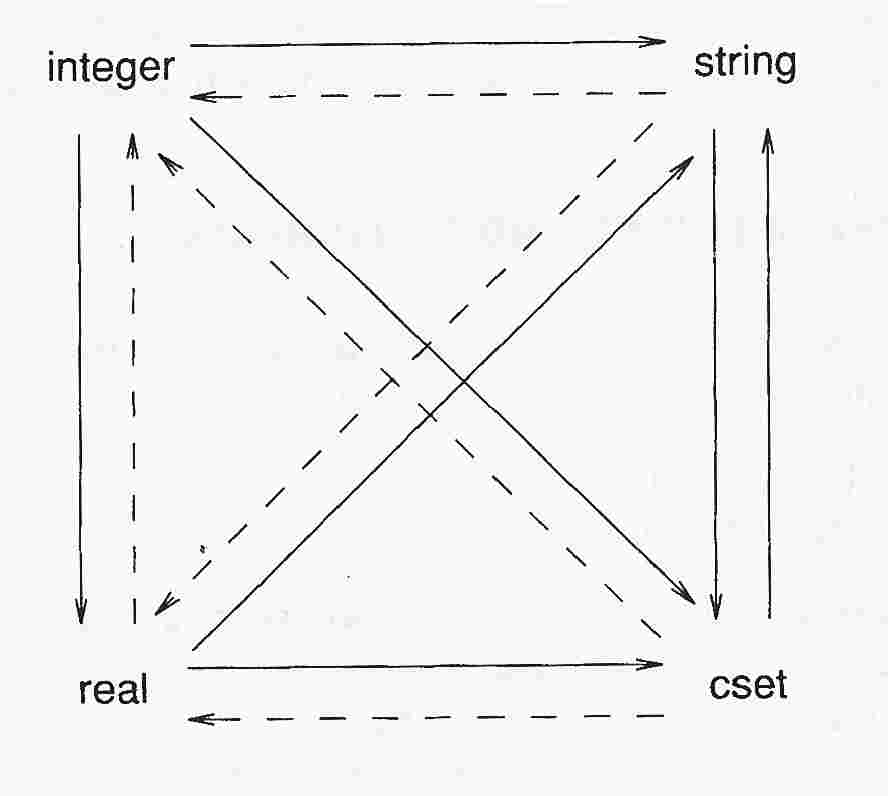
\includegraphics[width=2.9925in,height=2.6575in]{ib-img/ib-img105.jpg} 
% N.B. Can't have shorter dashed diagonal lines because LaTeX can't draw them
\begin{picture}(200,200)(-100,0)
\put(0,0){\makebox(0,0){\texttt{real}}}
\put(0,200){\makebox(0,0){\texttt{integer}}}
\put(200,0){\makebox(0,0){\texttt{cset}}}
\put(200,200){\makebox(0,0){\texttt{string}}}
\thicklines
\multiput(-4,-4)(0,200){2}{
\begin{picture}(0,0)
\put(30,10){\vector(1,0){150}}
\multiput(178,-3)(-24,0){6}{\line(-1,0){12}}\put(35,-3){\vector(-1,0){10}}
\end{picture}
}
\put(-5,170){\vector(0,-1){150}}
\multiput(10,20)(0,24){6}{\line(0,1){12}}\put(10,166){\vector(0,1){10}}
\put(190,170){\vector(0,-1){150}}
\put(205,20){\vector(0,1){150}}
\put(30,14){\vector(1,1){150}}
\multiput(30,35)(16,16){9}{\line(1,1){10}}\put(25,30){\vector(-1,-1){10}}
\multiput(170,20)(-16,16){9}{\line(-1,1){10}}\put(25,165){\vector(-1,1){10}}
\put(30,180){\vector(1,-1){150}}
\end{picture}

Thus, of the twelve conversions, five are conditional.

Some kinds of conversions are ``natural'' and occur frequently in
typical programs. Examples are string-to-integer conversion and
integer-to-string conversion. Other conversions, such as
cset-to-integer, are unlikely to occur in the normal course of
computation. To reduce the number of conversion routines required,
these unlikely conversions are done in two steps. For example, the
conversion of a cset to an integer is done by first converting the
cset to a string and then converting the string to an integer. The
direct conversions are

%--%\ \  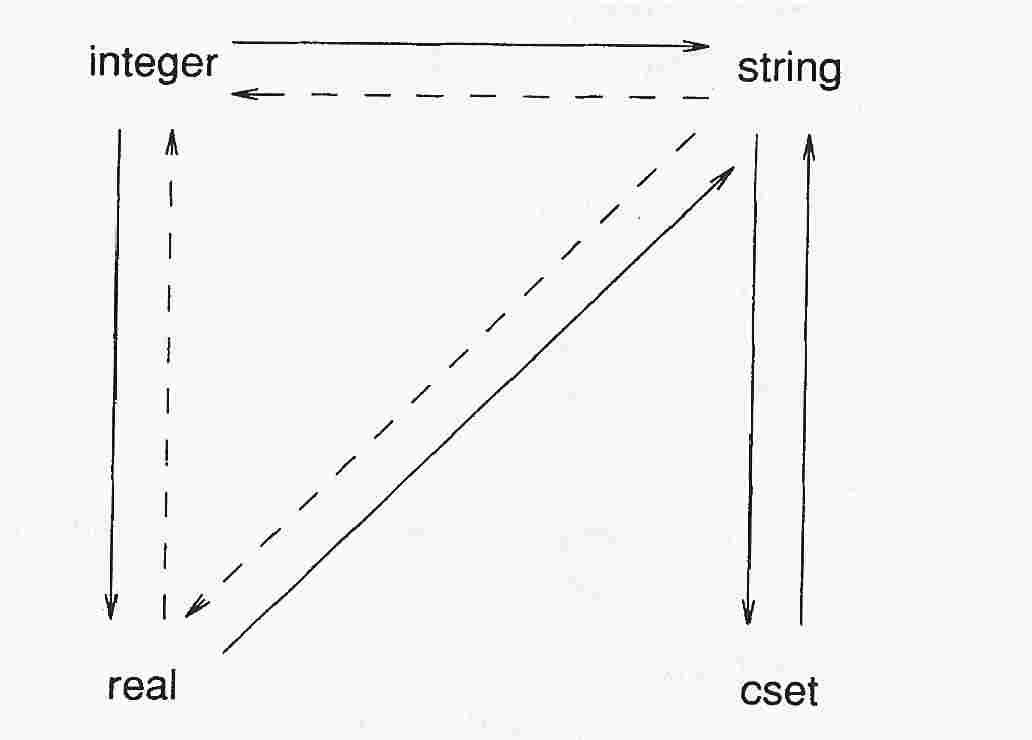
\includegraphics[width=3.5272in,height=2.4717in]{ib-img/ib-img106.jpg} 
% N.B. Can't have shorter dashed diagonal lines because LaTeX can't draw them
\begin{picture}(200,210)(-100,-10)
\put(0,0){\makebox(0,0){\texttt{real}}}
\put(0,200){\makebox(0,0){\texttt{integer}}}
\put(200,0){\makebox(0,0){\texttt{cset}}}
\put(200,200){\makebox(0,0){\texttt{string}}}
\thicklines
\put(30,206){\vector(1,0){150}}
\multiput(178,193)(-24,0){6}{\line(-1,0){12}}\put(35,193){\vector(-1,0){10}}
\put(-5,170){\vector(0,-1){150}}
\multiput(10,20)(0,24){6}{\line(0,1){12}}\put(10,166){\vector(0,1){10}}
\put(190,170){\vector(0,-1){150}}
\put(205,20){\vector(0,1){150}}
\put(30,14){\vector(1,1){150}}
\multiput(30,35)(16,16){9}{\line(1,1){10}}\put(25,30){\vector(-1,-1){10}}
\end{picture}

Conversions are done by calling routines that convert values to
expected types. These routines are

\begin{tabular}{l@{\hspace{1cm}}l}
\texttt{cnv\_cset} & convert to \texttt{cset}\\
\texttt{cnv\_int} & convert to \texttt{integer}\\
\texttt{cnv\_real} & convert to \texttt{real}\\
\texttt{cnv\_str} & convert to \texttt{string}\\
\end{tabular}

\noindent
Since these routines may be called with any type of value, all of them
are conditional. For example, it is not possible to convert a list to
a string. These routines return the value \texttt{CvtFail} to indicate
the failure of a conversion. If conversion is successful, they return
a value indicating the type of conversion.

Numerical computation introduces complications in addition to the
types integer and real, since there is the concept of a numeric
``type'' that includes both integers and real numbers. This is
represented explicitly by the Icon type-conversion function
\texttt{numeric(x)}, which converts \texttt{x} to either integer or
real, depending on the value of \texttt{x}. Its implementation
illustrates RTL's extensions to the C language for type conversions.
Rtt can generate special-case functions for each call to
\texttt{numeric(x)}, based on what it knows about the type information
at that call site, and skip the checks and conversions where they are
not necessary.

%-% {\ttfamily\mdseries
%-% function\{0,1\} numeric(n)}
%-% 
%-% {\ttfamily\mdseries
%-% \ \ \ if cnv:(exact)integer(n) then \{}
%-% 
%-% {\ttfamily\mdseries
%-% \ \ \ \ \ \ abstract \{ return integer \}}
%-% 
%-% {\ttfamily\mdseries
%-% \ \ \ \ \ \ inline \ \ \{ return n; \}}
%-% 
%-% {\ttfamily\mdseries
%-% \ \ \ \ \ \ \}}
%-% 
%-% {\ttfamily\mdseries
%-% \ \ \ else if cnv:real(n) then \{}
%-% 
%-% {\ttfamily\mdseries
%-% \ \ \ \ \ \ abstract \{ return real \}}
%-% 
%-% {\ttfamily\mdseries
%-% \ \ \ \ \ \ inline \ \ \{ return n; \}}
%-% 
%-% {\ttfamily\mdseries
%-% \ \ \ \ \ \ \}}
%-% 
%-% {\ttfamily\mdseries
%-% \ \ \ else \{}
%-% 
%-% {\ttfamily\mdseries
%-% \ \ \ \ \ \ abstract \{ return empty\_type \}}
%-% 
%-% {\ttfamily\mdseries
%-% \ \ \ \ \ \ inline \ \ \{ fail; \}}
%-% 
%-% {\ttfamily\mdseries
%-% \ \ \ \ \ \ \}}
%-% 
%-% {\ttfamily\mdseries
%-% end}
\goodbreak
\iconcode{
function\{0,1\} numeric(n)\\
\>if cnv:(exact)integer(n) then \{\\
\>\>abstract \{ return integer \}\\
\>\>inline \ \ \{ return n; \}\\
\>\>\}\\
\>else if cnv:real(n) then \{\\
\>\>abstract \{ return real \}\\
\>\>inline \ \ \{ return n; \}\\
\>\>\}\\
\>else \{\\
\>\>abstract \{ return empty\_type \}\\
\>\>inline \ \ \{ fail; \}\\
\>\>\}\\
end
}

Numeric conversion also occurs implicitly in polymorphic operations such as

{\ttfamily\mdseries
\ \ \ n+m}

\noindent which performs integer or real arithmetic, depending on the
types of \texttt{n} and \texttt{m}. The RTL language was given an
\texttt{arith\_case} construct specifically to handle this issue. The
general form of the arithmetic operators looks like:


%-% \ \ \ operator\{1\} icon\_op func\_name(x, y)
%-% 
%-% \ \ \ \ \ \ declare \{
%-% 
%-% \ \ \ \ \ \ \ \ \ tended struct descrip lx, ly;
%-% 
%-% \ \  C\_integer irslt;
%-% 
%-% \ \ \ \ \ \ \ \ \ \}
%-% 
%-% \ \ \ \ \ arith\_case (x, y) of \{
%-% 
%-% \ \ \ \ \ \ \ \ \ C\_integer: \{
%-% 
%-% \ \ \ \ \ \ \ \ \ \ \ \ abstract \{ return integer \}
%-% 
%-% \ \ \ \ \ \ \ \ \ \ \ \ inline \{
%-% 
%-% \ \ \ \ \ \ \ \ \ \ \ \ \ \ \ extern int over\_flow;
%-% 
%-% \ \ \ \ \ \ \ \ \ \ \ \ \ \ \ c\_int\_op(x,y);
%-% 
%-% \ \ \ \ \ \ \ \ \ \ \ \ \ \ \ \}
%-% 
%-% \ \ \ \ \ \ \ \ \ \ \ \ \}
%-% 
%-% \ \ \ \ \ \ \ \ \ integer: \{ /* large integers only */
%-% 
%-% \ \ \ \ \ \ \ \ \ \ \ \ abstract \{ return integer \}
%-% 
%-% \ \ \ \ \ \ \ \ \ \ \ \ inline \{
%-% 
%-% \ \ \ \ \ \ \ \ \ \ \ \ \ \ \ big\_ \#\# c\_int\_op(x,y);
%-% 
%-% \ \ \ \ \ \ \ \ \ \ \ \ \ \ \ \}
%-% 
%-% \ \ \ \ \ \ \ \ \ \ \ \ \}
%-% 
%-% \ \ \ \ \ \ \ \ \ C\_double: \{
%-% 
%-% \ \ \ \ \ \ \ \ \ \ \ \ abstract \{ return real \}
%-% 
%-% \ \ \ \ \ \ \ \ \ \ \ \ inline \{
%-% 
%-% \ \ \ \ \ \ \ \ \ \ \ \ \ \ \ c\_real\_op(x, y);
%-% 
%-% \ \ \ \ \ \ \ \ \ \ \ \ \ \ \ \}
%-% 
%-% \ \ \ \ \ \ \ \ \ \ \ \ \}
%-% 
%-% \ \ \ \ \ \ \ \ \ \}
%-% 
%-% \ \ \ end
\goodbreak
\iconcode{
\>operator\{1\} icon\_op func\_name(x, y)\\
\>\>declare \{\\
\>\>\>tended struct descrip lx, ly;\\
\ \  C\_integer irslt;\\
\>\>\>\}\\
\>\ \ arith\_case (x, y) of \{\\
\>\>\>C\_integer: \{\\
\>\>\>\>abstract \{ return integer \}\\
\>\>\>\>inline \{\\
\>\>\>\>\>extern int over\_flow;\\
\>\>\>\>\>c\_int\_op(x,y);\\
\>\>\>\>\>\}\\
\>\>\>\>\}\\
\>\>\>integer: \{ /* large integers only */\\
\>\>\>\>abstract \{ return integer \}\\
\>\>\>\>inline \{\\
\>\>\>\>\>big\_\#\# c\_int\_op(x,y);\\
\>\>\>\>\>\}\\
\>\>\>\>\}\\
\>\>\>C\_double: \{\\
\>\>\>\>abstract \{ return real \}\\
\>\>\>\>inline \{\\
\>\>\>\>\>c\_real\_op(x, y);\\
\>\>\>\>\>\}\\
\>\>\>\>\}\\
\>\>\>\}\\
\>end
}

Internally, a macro \texttt{GetReal()} is used to handle the \texttt{real}
type, since some computers have restrictions on the alignment of
\texttt{double}s. Thus, \texttt{GetReal()} has different definitions depending
on the target computer. The actual conversion of a string to a numeric
value is done by \texttt{ston()}. Note that the conversion of a cset
to a numeric value occurs by way of conversion to a string.

When types are not known at compile-time, RTL constructs such as
\texttt{cnv:str(d)} are translated down to conversion routines in
cnv.r. String conversion requires a buffer to construct the string. In
a common special-case, this buffer is provided by the routine that is
requesting string conversion for temporary use, avoiding the heap
memory allocator.  This is used, for example when a value is converted
to a string in order to convert it to a number. See Sec. 4.4.4. The
code for the ``temporary string'' version of string conversion is in a
function \texttt{tmp\_str()}:

%-% {\ttfamily\mdseries
%-% static int tmp\_str(char *sbuf, dptr s, dptr d)}
%-% 
%-% {\ttfamily\mdseries
%-% \ \ \ \{}
%-% 
%-% {\ttfamily\mdseries
%-% \ \ \ type\_case *s of \{}
%-% 
%-% {\ttfamily\mdseries
%-% \ \ \ \ \ \ string:}
%-% 
%-% {\ttfamily\mdseries
%-% \ \ \ \ \ \ \ \ \ *d = *s;}
%-% 
%-% {\ttfamily\mdseries
%-% \ \ \ \ \ \ integer: \{}
%-% 
%-% {\ttfamily\mdseries
%-% \ \ \ \ \ \ \ \ \ if (Type(*s) == T\_Lrgint) \{}
%-% 
%-% {\ttfamily\mdseries
%-% \ \ \ \ \ \ \ \ \ \ \ \ word slen, dlen;}
%-% 
%-% {\ttfamily\mdseries
%-% \ \ \ \ \ \ \ \ \ \ \ \ slen = (BlkLoc(*s)-{\textgreater}bignumblk.lsd -}
%-% 
%-% {\ttfamily\mdseries
%-% \ \ \ \ \ \ \ \ \ \ \ \ \ \ \ \ \ \ \ \ BlkLoc(*s)-{\textgreater}bignumblk.msd +1);}
%-% 
%-% {\ttfamily\mdseries
%-% \ \ \ \ \ \ \ \ \ \ \ \ dlen=slen * NB * 0.3010299956639812; /* 1/log2(10) */}
%-% 
%-% {\ttfamily\mdseries
%-% \ \ \ \ \ \ \ \ \ \ \ \ bigtos(s,d);}
%-% 
%-% {\ttfamily\mdseries
%-% \ \ \ \ \ \ \ \ \ \ \ \ \}}
%-% 
%-% {\ttfamily\mdseries
%-% \ \ \ \ \ \ \ \ \ else}
%-% 
%-% {\ttfamily\mdseries
%-% \ \ \ \ \ \ \ \ \ \ \ \ itos(IntVal(*s), d, sbuf);}
%-% 
%-% {\ttfamily\mdseries
%-% \ \ \ \ \ \ \ \ \ \}}
%-% 
%-% {\ttfamily\mdseries
%-% \ \ \ \ \ \ real: \{}
%-% 
%-% {\ttfamily\mdseries
%-% \ \ \ \ \ \ \ \ \ double res;}
%-% 
%-% {\ttfamily\mdseries
%-% \ \ \ \ \ \ \ \ \ GetReal(s, res);}
%-% 
%-% {\ttfamily\mdseries
%-% \ \ \ \ \ \ \ \ \ rtos(res, d, sbuf);}
%-% 
%-% {\ttfamily\mdseries
%-% \ \ \ \ \ \ \ \ \ \}}
%-% 
%-% {\ttfamily\mdseries
%-% \ \ \ \ \ \ cset:}
%-% 
%-% {\ttfamily\mdseries
%-% \ \ \ \ \ \ \ \ \ cstos(BlkLoc(*s)-{\textgreater}cset.bits, d, sbuf);}
%-% 
%-% {\ttfamily\mdseries
%-% \ \ \ \ \ \ default:}
%-% 
%-% {\ttfamily\mdseries
%-% \ \ \ \ \ \ \ \ \ return 0;}
%-% 
%-% {\ttfamily\mdseries
%-% \ \ \ \ \ \ \}}
%-% 
%-% {\ttfamily\mdseries
%-% \ \ \ return 1;}
%-% 
%-% {\ttfamily\mdseries
%-% \ \ \ \}}
\goodbreak
\iconcode{
static int tmp\_str(char *sbuf, dptr s, dptr d)\\
\>\{\\
\>type\_case *s of \{\\
\>\>string:\\
\>\>\>*d = *s;\\
\>\>integer: \{\\
\>\>\>if (Type(*s) == T\_Lrgint) \{\\
\>\>\>\>word slen, dlen;\\
\>\>\>\>slen = (BlkLoc(*s)->bignumblk.lsd -\\
\>\>\>\>\>\>\ \ BlkLoc(*s)->bignumblk.msd +1);\\
\>\>\>\>dlen=slen * NB * 0.3010299956639812; /* 1/log2(10) */\\
\>\>\>\>bigtos(s,d);\\
\>\>\>\>\}\\
\>\>\>else\\
\>\>\>\>itos(IntVal(*s), d, sbuf);\\
\>\>\>\}\\
\>\>real: \{\\
\>\>\>double res;\\
\>\>\>GetReal(s, res);\\
\>\>\>rtos(res, d, sbuf);\\
\>\>\>\}\\
\>\>cset:\\
\>\>\>cstos(BlkLoc(*s)->cset.bits, d, sbuf);\\
\>\>default:\\
\>\>\>return 0;\\
\>\>\}\\
\>return 1;\\
\>\}
}

If a conversion is required, \texttt{itos()}, \texttt{rtos()}, or
\texttt{cstos()} does the actual work, placing its result in \texttt{sbuf} and
changing the descriptor pointed to by \texttt{d} accordingly. These routines
return a 1 if the result is a string and a 0 otherwise. The monitoring
facilities in Unicon can also report whether no conversion was needed
(\texttt{E\_Nconv}), a conversion was performed successfully
(\texttt{E\_Sconv}), or the conversion failed (\texttt{E\_Fconv}).

If a converted string is in a buffer that is local to the calling
routine, it must be copied into allocated storage, or it would be
destroyed when that routine returns. The fully general version of
\texttt{cnv\_str()} is equivalent to the following function. Because
this function is heavily called, in reality the body of
\texttt{tmp\_str()} is inlined in \texttt{cnv\_str()}.

%-% {\ttfamily\mdseries
%-% int cnv\_str(dptr s, dptr d)}
%-% 
%-% {\ttfamily\mdseries
%-% \ \ \ \{}
%-% 
%-% {\ttfamily\mdseries
%-% \ \ \ char sbuf[MaxCvtLen];}
%-% 
%-% 
%-% \bigskip
%-% 
%-% {\ttfamily\mdseries
%-% \ \ \ type\_case *s of \{}
%-% 
%-% {\ttfamily\mdseries
%-% \ \ \ \ \ \ string: \{}
%-% 
%-% {\ttfamily\mdseries
%-% \ \ \ \ \ \ \ \ \ *d = *s;}
%-% 
%-% {\ttfamily\mdseries
%-% \ \ \ \ \ \ \ \ \ return 1;}
%-% 
%-% {\ttfamily\mdseries
%-% \ \ \ \ \ \ \ \ \ \}}
%-% 
%-% {\ttfamily\mdseries
%-% \ \ \ \ \ \ default: \{}
%-% 
%-% {\ttfamily\mdseries
%-% \ \ \ \ \ \ \ \ \ if (!tmp\_str(sbuf, s, d)) return 0;}
%-% 
%-% {\ttfamily\mdseries
%-% \ \ \ \ \ \ \ \ \ \}}
%-% 
%-% {\ttfamily\mdseries
%-% \ \ \ \ \ \ \}}
%-% 
%-% {\ttfamily\mdseries
%-% \ \ \ Protect(StrLoc(*d) =}
%-% 
%-% {\ttfamily\mdseries
%-% \ \ \ \ \ \ \ \ \ \ \ \ \ \ alcstr(StrLoc(*d), StrLen(*d)), fatalerr(0,NULL));}
%-% 
%-% {\ttfamily\mdseries
%-% \ \ \ return 1;}
%-% 
%-% {\ttfamily\mdseries
%-% \ \ \ \}}
\goodbreak
\iconcode{
int cnv\_str(dptr s, dptr d)\\
\>\{\\
\>char sbuf[MaxCvtLen];\\
\\
\>type\_case *s of \{\\
\>\>string: \{\\
\>\>\>*d = *s;\\
\>\>\>return 1;\\
\>\>\>\}\\
\>\>default: \{\\
\>\>\>if (!tmp\_str(sbuf, s, d)) return 0;\\
\>\>\>\}\\
\>\>\}\\
\>Protect(StrLoc(*d) = alcstr(StrLoc(*d), StrLen(*d)), fatalerr(0,NULL));\\
\>return 1;\\
\>\}
}

\section[12.2 Dereferencing and Assignment]{12.2 Dereferencing and Assignment}

If there were no trapped or keyword variables, dereferencing and assignment would
be trivial. For example, the descriptor \texttt{d} is dereferenced by

%-% {\ttfamily\mdseries
%-% \ \ \ d = *VarLoc(d)}
\iconline{ \>d = *VarLoc(d) }

\noindent where \texttt{VarLoc} references the v-word of \texttt{d}:

%-% {\ttfamily\mdseries
%-% \ \ \ \#define VarLoc(d) ((d).vword.dptr)}
\iconline{\>\#define VarLoc(d) ((d).vword.dptr) }

The dereferencing or assignment to a trapped variable, on the other
hand, may involve a complicated computation. This computation reflects
the meaning associated with the operation on the source-language
expression that is represented in the implementation as a trapped
variable. For example, as discussed previously, in

%-% {\ttfamily\mdseries
%-% \textit{\ \ \ }x[y] := z}
\iconline{ \textit{\ \ \ }x[y] := z }

\noindent the value of \texttt{x} may be a list, a string, a table, or a
record. A subscripted list or record does not produce a trapped
variable, but the other two cases do. For a string, the variable on
the left side of the assignment is a substring trapped variable. For a
table, the variable is a table-element trapped variable. In the first
case, the assignment involves the concatenation of three strings and
the assignment of the result to \texttt{x}. In the second case, it involves
looking for \texttt{y} in the table. If there is a table element for \texttt{y}, its
assigned value is changed to the value of \texttt{z}.  Otherwise, the
table-element trapped-variable block is converted to a table-element
block with the assigned value, and the block is inserted in the
appropriate chain.

\subsection[12.2.1 Dereferencing]{12.2.1 Dereferencing}

Dereferencing of other trapped variables involves computations of
comparable complexity. Dereferencing is done in the interpreter loop
for arguments of operators for which variables are not needed. For
example, in

%-% {\ttfamily\mdseries
%-% \ \ \ n+m}
\iconline{ \>n+m }

\noindent the identifiers \texttt{n} and \texttt{m} are dereferenced before the function
for addition is called (See Sec. 8.3.1). On the other hand, in

{\ttfamily\mdseries
\ \ \ s[i]}

\noindent the identifier \texttt{i} is dereferenced, but \texttt{s} is not, since the
subscripting routine needs the variable as well as its value.

The function invocation routine also dereferences variables before a
function is called. Note that there is no function that requires an
argument that is a variable. Suspension and return from procedures
also dereference local identifiers and arguments. Dereferencing occurs
in a number of other places. For example, the function that handles
subscripting must dereference the subscripted variable to determine
what kind of result to produce.

The dereferencing routine begins as follows:

%-% {\ttfamily\mdseries
%-% void deref(s, d)}
%-% 
%-% {\ttfamily\mdseries
%-% dptr s, d;}
%-% 
%-% {\ttfamily\mdseries
%-% \ \ \ \{}
%-% 
%-% {\ttfamily\mdseries
%-% \ \ \ /*}
%-% 
%-% {\ttfamily\mdseries
%-% \ \ \ \ * no allocation is done, so nothing need be tended.}
%-% 
%-% {\ttfamily\mdseries
%-% \ \ \ \ */}
%-% 
%-% {\ttfamily\mdseries
%-% \ \ \ register union block *bp, **ep;}
%-% 
%-% {\ttfamily\mdseries
%-% \ \ \ struct descrip v;}
%-% 
%-% {\ttfamily\mdseries
%-% \ \ \ int res;}
%-% 
%-% 
%-% \bigskip
%-% 
%-% {\ttfamily\mdseries
%-% \ \ \ if (!is:variable(*s)) \{}
%-% 
%-% {\ttfamily\mdseries
%-% \ \ \ \ \ \ *d = *s;}
%-% 
%-% {\ttfamily\mdseries
%-% \ \ \ \ \ \ \}}
\goodbreak
\iconcode{
void deref(s, d)\\
dptr s, d;\\
\>\{\\
\>/*\\
\>\ * no allocation is done, so nothing need be tended.\\
\>\ */\\
\>register union block *bp, **ep;\\
\>struct descrip v;\\
\>int res;\\
\\
\>if (!is:variable(*s)) \{\\
\>\>*d = *s;\\
\>\>\}
}


\noindent
If \texttt{s} does not point to a variable descriptor, the remaining code is skipped.

If \texttt{s} points to a variable that is not a trapped variable,
dereferencing is simple:

%-% {\ttfamily\mdseries
%-% \ \ \ \ \ \ \ \ \ /*}
%-% 
%-% {\ttfamily\mdseries
%-% \ \ \ \ \ \ \ \ \ \ * An ordinary variable is being dereferenced.}
%-% 
%-% {\ttfamily\mdseries
%-% \ \ \ \ \ \ \ \ \ \ */}
%-% 
%-% {\ttfamily\mdseries
%-% \ \ \ \ \ \ \ \ \ *d = *(dptr)((word *)VarLoc(*s) + Offset(*s));}
\goodbreak
\iconcode{
\>\>\>/*\\
\>\>\>\ * An ordinary variable is being dereferenced.\\
\>\>\>\ */\\
\>\>\>*d = *(dptr)((word *)VarLoc(*s) + Offset(*s));
}

Otherwise, there are two types of trapped variables with a switch on the type:

%-% {\ttfamily\mdseries
%-% \ \ \ type\_case *s of \{}
%-% 
%-% {\ttfamily\mdseries
%-% \ \ \ \ \ \ tvsubs: \{}
%-% 
%-% {\ttfamily\mdseries
%-% \ \ \ \ \ \ \ \ \ /*}
%-% 
%-% {\ttfamily\mdseries
%-% \ \ \ \ \ \ \ \ \ \ * A substring trapped variable is being dereferenced.}
%-% 
%-% {\ttfamily\mdseries
%-% \ \ \ \ \ \ \ \ \ \ * \ Point bp to the trapped variable block and v to}
%-% 
%-% {\ttfamily\mdseries
%-% \ \ \ \ \ \ \ \ \ \ * \ the string.}
%-% 
%-% {\ttfamily\mdseries
%-% \ \ \ \ \ \ \ \ \ \ */}
%-% 
%-% {\ttfamily\mdseries
%-% \ \ \ \ \ \ \ \ \ bp = BlkLoc(*s);}
%-% 
%-% {\ttfamily\mdseries
%-% \ \ \ \ \ \ \ \ \ deref(\&bp-{\textgreater}tvsubs.ssvar, \&v);}
%-% 
%-% {\ttfamily\mdseries
%-% \ \ \ \ \ \ \ \ \ if (!is:string(v))}
%-% 
%-% {\ttfamily\mdseries
%-% \ \ \ \ \ \ \ \ \ \ \ \ fatalerr(103, \&v);}
%-% 
%-% {\ttfamily\mdseries
%-% \ \ \ \ \ \ \ \ \ if (bp-{\textgreater}tvsubs.sspos + bp-{\textgreater}tvsubs.sslen - 1 {\textgreater} StrLen(v))}
%-% 
%-% {\ttfamily\mdseries
%-% \ \ \ \ \ \ \ \ \ \ \ \ fatalerr(205, NULL);}
%-% 
%-% {\ttfamily\mdseries
%-% \ \ \ \ \ \ \ \ \ /*}
%-% 
%-% {\ttfamily\mdseries
%-% \ \ \ \ \ \ \ \ \ \ * Make a descriptor for the substring by getting the}
%-% 
%-% {\ttfamily\mdseries
%-% \ \ \ \ \ \ \ \ \ \ * \ length and pointing into the string.}
%-% 
%-% {\ttfamily\mdseries
%-% \ \ \ \ \ \ \ \ \ \ */}
%-% 
%-% {\ttfamily\mdseries
%-% \ \ \ \ \ \ \ \ \ StrLen(*d) = bp-{\textgreater}tvsubs.sslen;}
%-% 
%-% {\ttfamily\mdseries
%-% \ \ \ \ \ \ \ \ \ StrLoc(*d) = StrLoc(v) + bp-{\textgreater}tvsubs.sspos - 1;}
%-% 
%-% {\ttfamily\mdseries
%-% \ \ \ \ \ \ \ \ \}}
%-% 
%-% 
%-% \bigskip
%-% 
%-% {\ttfamily\mdseries
%-% \ \ \ \ \ \ tvtbl: \{}
%-% 
%-% {\ttfamily\mdseries
%-% \ \ \ \ \ \ \ \ \ /*}
%-% 
%-% {\ttfamily\mdseries
%-% \ \ \ \ \ \ \ \ \ \ * Look up the element in the table.}
%-% 
%-% {\ttfamily\mdseries
%-% \ \ \ \ \ \ \ \ \ \ */}
%-% 
%-% {\ttfamily\mdseries
%-% \ \ \ \ \ \ \ \ \ bp = BlkLoc(*s);}
%-% 
%-% {\ttfamily\mdseries
%-% \ \ \ \ \ \ \ \ \ ep = memb(bp-{\textgreater}tvtbl.clink,\&bp-{\textgreater}tvtbl.tref,}
%-% 
%-% {\ttfamily\mdseries
%-% \ \ \ \ \ \ \ \ \ \ \ \ \ \ \ \ \ \ \ bp-{\textgreater}tvtbl.hashnum,\&res);}
%-% 
%-% {\ttfamily\mdseries
%-% \ \ \ \ \ \ \ \ \ if (res == 1)}
%-% 
%-% {\ttfamily\mdseries
%-% \ \ \ \ \ \ \ \ \ \ \ \ *d = (*ep)-{\textgreater}telem.tval;\ \ /* found; use value */}
%-% 
%-% {\ttfamily\mdseries
%-% \ \ \ \ \ \ \ \ \ else}
%-% 
%-% {\ttfamily\mdseries
%-% \ \ \ \ \ \ \ \ \ \ \ \ *d = bp-{\textgreater}tvtbl.clink-{\textgreater}table.defvalue;/*use default */}
%-% 
%-% {\ttfamily\mdseries
%-% \ \ \ \ \ \ \ \ \ \}}
\goodbreak
\iconcode{
\>type\_case *s of \{\\
\>\>tvsubs: \{\\
\>\>\>/*\\
\>\>\>\ * A substring trapped variable is being dereferenced.\\
\>\>\>\ * \ Point bp to the trapped variable block and v to\\
\>\>\>\ * \ the string.\\
\>\>\>\ */\\
\>\>\>bp = BlkLoc(*s);\\
\>\>\>deref(\&bp->tvsubs.ssvar, \&v);\\
\>\>\>if (!is:string(v))\\
\>\>\>\>fatalerr(103, \&v);\\
\>\>\>if (bp->tvsubs.sspos + bp->tvsubs.sslen - 1 > StrLen(v))\\
\>\>\>\>fatalerr(205, NULL);\\
\>\>\>/*\\
\>\>\>\ * Make a descriptor for the substring by getting the\\
\>\>\>\ * \ length and pointing into the string.\\
\>\>\>\ */\\
\>\>\>StrLen(*d) = bp->tvsubs.sslen;\\
\>\>\>StrLoc(*d) = StrLoc(v) + bp->tvsubs.sspos - 1;\\
\>\>\ \ \}\\
\\
\>\>tvtbl: \{\\
\>\>\>/*\\
\>\>\>\ * Look up the element in the table.\\
\>\>\>\ */\\
\>\>\>bp = BlkLoc(*s);\\
\>\>\>ep = memb(bp->tvtbl.clink,\&bp->tvtbl.tref,\\
\>\>\>\>\>\>\ bp->tvtbl.hashnum,\&res);\\
\>\>\>if (res == 1)\\
\>\>\>\>*d = (*ep)->telem.tval;\ \ /* found; use value */\\
\>\>\>else\\
\>\>\>\>*d = bp->tvtbl.clink->table.defvalue;/*use default */\\
\>\>\>\}
}

A table-element trapped variable may point to a table-element
trapped-variable block or to a table-element block. The second
situation occurs if two table-element trapped variables point to the
same table-element trapped-variable block and assignment to one of the
variables converts the table-element trapped-variable block to a
table-element block before the second variable is processed. See
Sec. 7.2. In this case, the value of the trapped variable is in the
table-element block. On the other hand, if the trapped variable points
to a table-element trapped-variable block, it is necessary to look up
the subscripting value in the table, since an assignment for it may
have been made between the time the trapped variable was created and
the time it was dereferenced. If it is in the table, the corresponding
assigned value is returned. If it is not in the table, the default
assigned value is returned.

The last case, keyword variables, is almost the same as for
simple variables. These variables impose special semantics on
assignment, but not on dereferencing.

%-% {\ttfamily\mdseries
%-% \ \ \ \ \ \ kywdint:}
%-% 
%-% {\ttfamily\mdseries
%-% \ \ \ \ \ \ kywdpos:}
%-% 
%-% {\ttfamily\mdseries
%-% \ \ \ \ \ \ kywdsubj:}
%-% 
%-% {\ttfamily\mdseries
%-% \ \ \ \ \ \ kywdevent:}
%-% 
%-% {\ttfamily\mdseries
%-% \ \ \ \ \ \ kywdwin:}
%-% 
%-% {\ttfamily\mdseries
%-% \ \ \ \ \ \ kywdstr:}
%-% 
%-% 
%-% \ \ \ \ \ \ \ \ \ *d = *VarLoc(*s);
\goodbreak
\iconcode{
\>\>kywdint:\\
\>\>kywdpos:\\
\>\>kywdsubj:\\
\>\>kywdevent:\\
\>\>kywdwin:\\
\>\>kywdstr:\\
\>\>\>*d = *VarLoc(*s);
}

\subsection[12.2.2 Assignment]{12.2.2 Assignment}

The values of global identifiers are established initially as a
byproduct of reading the icode file into the icode region. When
procedures are called, the values of arguments and local identifiers
are on the interpreter stack. These operations associate values with
variables, but assignment, unlike dereferencing, is explicit in the
source program.


The macro \texttt{GeneralAsgn()} is used to perform all such
operations. For example, the function for

%-% {\ttfamily\mdseries
%-% \ \ \ x := y}
\iconline{ \>x := y }

is

%-% {\ttfamily\mdseries
%-% operator\{0,1\} := asgn(underef x, y)}
%-% 
%-% {\ttfamily\mdseries
%-% \ \ \ if !is:variable(x) then}
%-% 
%-% {\ttfamily\mdseries
%-% \ \ \ \ \ \ runerr(111, x)}
%-% 
%-% {\ttfamily\mdseries
%-% \ \ \ abstract \{}
%-% 
%-% {\ttfamily\mdseries
%-% \ \ \ \ \ \ return type(x)}
%-% 
%-% {\ttfamily\mdseries
%-% \ \ \ \ \ \ \}}
%-% 
%-% {\ttfamily\mdseries
%-% \ \ \ GeneralAsgn(x, y)}
%-% 
%-% {\ttfamily\mdseries
%-% \ \ \ inline \{}
%-% 
%-% {\ttfamily\mdseries
%-% \ \ \ \ \ \ /*}
%-% 
%-% {\ttfamily\mdseries
%-% \ \ \ \ \ \ \ * The returned result is the variable to which assignment }
%-% 
%-% {\ttfamily\mdseries
%-% \ \ \ \ \ \ \ * \ is being made.}
%-% 
%-% {\ttfamily\mdseries
%-% \ \ \ \ \ \ \ */}
%-% 
%-% {\ttfamily\mdseries
%-% \ \ \ \ \ \ return x;}
%-% 
%-% {\ttfamily\mdseries
%-% \ \ \ \ \ \ \}}
%-% 
%-% {\ttfamily\mdseries
%-% end}
\goodbreak
\iconcode{
operator\{0,1\} := asgn(underef x, y)\\
\>if !is:variable(x) then\\
\>\>runerr(111, x)\\
\>abstract \{\\
\>\>return type(x)\\
\>\>\}\\
\>GeneralAsgn(x, y)\\
\>inline \{\\
\>\>/*\\
\>\>\ * The returned result is the variable to which assignment \\
\>\>\ * \ is being made.\\
\>\>\ */\\
\>\>return x;\\
\>\>\}\\
end
}

Note that assignment may fail. This can occur as the result of an
out-of-range assignment to \texttt{\&pos} and is indicated by an RTL
\texttt{fail} statement from within \texttt{GeneralAsgn()}.

Like dereferencing, assignment is trivial for variables that are not
trapped. The macro \texttt{GeneralAsgn()} begins as follows:

%-% {\ttfamily\mdseries
%-% \#begdef GeneralAsgn(x, y)}
%-% 
%-% \bigskip
%-% 
%-% {\ttfamily\mdseries
%-% \ \ \ type\_case x of \{}
\goodbreak
\iconcode{
\#begdef GeneralAsgn(x, y)\\
\>type\_case x of \{
}

As for dereferencing, there are two types of trapped variables to be
considered. Assignment to a substring trapped variable is rather
complicated and deferred to a function \texttt{subs\_asgn()}:

%-% {\ttfamily\mdseries
%-% \ \ \ \ \ \ tvsubs: \{}
%-% 
%-% {\ttfamily\mdseries
%-% \ \ \ \ \ \ \ \ abstract \{}
%-% 
%-% {\ttfamily\mdseries
%-% \ \ \ \ \ \ \ \ \ \ \ store[store[type(x).str\_var]] = string}
%-% 
%-% {\ttfamily\mdseries
%-% \ \ \ \ \ \ \ \ \ \ \ \}}
%-% 
%-% {\ttfamily\mdseries
%-% \ \ \ \ \ \ \ \ inline \{}
%-% 
%-% {\ttfamily\mdseries
%-% \ \ \ \ \ \ \ \ \ \ \ if (subs\_asgn(\&x, (const dptr)\&y) == Error)}
%-% 
%-% {\ttfamily\mdseries
%-% \ \ \ \ \ \ \ \ \ \ \ \ \ \ runerr(0);}
%-% 
%-% {\ttfamily\mdseries
%-% \ \ \ \ \ \ \ \ \ \ \ \}}
%-% 
%-% {\ttfamily\mdseries
%-% \ \ \ \ \ \ \ \ \}}
\goodbreak
\iconcode{
\>\>tvsubs: \{\\
\>\>\ \ abstract \{\\
\>\>\>\ \ store[store[type(x).str\_var]] = string\\
\>\>\>\ \ \}\\
\>\>\ \ inline \{\\
\>\>\>\ \ if (subs\_asgn(\&x, (const dptr)\&y) == Error)\\
\>\>\>\>\ \ runerr(0);\\
\>\>\>\ \ \}\\
\>\>\ \ \}
}

The function \texttt{subs\_asgn()}:

%-% {\ttfamily\mdseries
%-% int subs\_asgn(dptr dest, const dptr src)}
%-% 
%-% {\ttfamily\mdseries
%-% \ \ \ \{}
%-% 
%-% {\ttfamily\mdseries
%-% \ \ \ tended struct descrip deststr, srcstr, rsltstr;}
%-% 
%-% {\ttfamily\mdseries
%-% \ \ \ tended struct b\_tvsubs *tvsub;}
%-% 
%-% 
%-% \bigskip
%-% 
%-% {\ttfamily\mdseries
%-% \ \ \ char *s, *s2;}
%-% 
%-% {\ttfamily\mdseries
%-% \ \ \ word i, len;}
%-% 
%-% {\ttfamily\mdseries
%-% \ \ \ word prelen;/* length of portion of string before substring */}
%-% 
%-% {\ttfamily\mdseries
%-% \ \ \ word poststrt, postlen; /* start and length of portion of}
%-% 
%-% {\ttfamily\mdseries
%-% \ \ \ \ \ \ \ \ \ \ \ \ \ \ \ \ \ \ \ \ \ \ \ \ \ \ \ \ \ \ string following substring */}
%-% 
%-% {\ttfamily\mdseries
%-% \ \ \ if (!cnv:tmp\_string(*src, srcstr))}
%-% 
%-% {\ttfamily\mdseries
%-% \ \ \ \ \ \ ReturnErrVal(103, *src, Error);}
%-% 
%-% {\ttfamily\mdseries
%-% \ \ \ /*}
%-% 
%-% {\ttfamily\mdseries
%-% \ \ \ \ * Be sure that the variable in the trapped variable points}
%-% 
%-% {\ttfamily\mdseries
%-% \ \ \ \ * \ to a string and that the string is big enough to contain}
%-% 
%-% {\ttfamily\mdseries
%-% \ \ \ \ * \ the substring.}
%-% 
%-% {\ttfamily\mdseries
%-% \ \ \ \ */}
%-% 
%-% {\ttfamily\mdseries
%-% \ \ \ tvsub = (struct b\_tvsubs *)BlkLoc(*dest);}
%-% 
%-% {\ttfamily\mdseries
%-% \ \ \ deref(\&tvsub-{\textgreater}ssvar, \&deststr);}
%-% 
%-% {\ttfamily\mdseries
%-% \ \ \ if (!is:string(deststr))}
%-% 
%-% {\ttfamily\mdseries
%-% \ \ \ \ \ \ ReturnErrVal(103, deststr, Error);}
%-% 
%-% {\ttfamily\mdseries
%-% \ \ \ prelen = tvsub-{\textgreater}sspos - 1;}
%-% 
%-% {\ttfamily\mdseries
%-% \ \ \ poststrt = prelen + tvsub-{\textgreater}sslen;}
%-% 
%-% {\ttfamily\mdseries
%-% \ \ \ if (poststrt {\textgreater} StrLen(deststr))}
%-% 
%-% {\ttfamily\mdseries
%-% \ \ \ \ \ \ ReturnErrNum(205, Error);}
%-% 
%-% 
%-% \bigskip
%-% 
%-% {\ttfamily\mdseries
%-% \ \ \ /*}
%-% 
%-% {\ttfamily\mdseries
%-% \ \ \ \ * Form the result string.}
%-% 
%-% {\ttfamily\mdseries
%-% \ \ \ \ * \ Start by allocating space for the entire result.}
%-% 
%-% {\ttfamily\mdseries
%-% \ \ \ \ */}
%-% 
%-% {\ttfamily\mdseries
%-% \ \ \ len = prelen + StrLen(srcstr) + StrLen(deststr) - poststrt;}
%-% 
%-% {\ttfamily\mdseries
%-% \ \ \ Protect(s = alcstr(NULL, len), return Error);}
%-% 
%-% {\ttfamily\mdseries
%-% \ \ \ StrLoc(rsltstr) = s;}
%-% 
%-% {\ttfamily\mdseries
%-% \ \ \ StrLen(rsltstr) = len;}
%-% 
%-% {\ttfamily\mdseries
%-% \ \ \ /*}
%-% 
%-% {\ttfamily\mdseries
%-% \ \ \ \ * First, copy the portion of the substring string to}
%-% 
%-% {\ttfamily\mdseries
%-% \ \ \ \ * \ the left of the substring into the string space.}
%-% 
%-% {\ttfamily\mdseries
%-% \ \ \ \ */}
%-% 
%-% {\ttfamily\mdseries
%-% \ \ \ s2 = StrLoc(deststr);}
%-% 
%-% {\ttfamily\mdseries
%-% \ \ \ for (i = 0; i {\textless} prelen; i++)}
%-% 
%-% {\ttfamily\mdseries
%-% \ \ \ \ \ \ *s++ = *s2++;}
%-% 
%-% {\ttfamily\mdseries
%-% \ \ \ /*}
%-% 
%-% {\ttfamily\mdseries
%-% \ \ \ \ * Copy the string to be assigned into the string space,}
%-% 
%-% {\ttfamily\mdseries
%-% \ \ \ \ * \ effectively concatenating it.}
%-% 
%-% {\ttfamily\mdseries
%-% \ \ \ \ */}
%-% 
%-% {\ttfamily\mdseries
%-% \ \ \ s2 = StrLoc(srcstr);}
%-% 
%-% {\ttfamily\mdseries
%-% \ \ \ for (i = 0; i {\textless} StrLen(srcstr); i++)}
%-% 
%-% {\ttfamily\mdseries
%-% \ \ \ \ \ \ *s++ = *s2++;}
%-% 
%-% {\ttfamily\mdseries
%-% \ \ \ /*}
%-% 
%-% {\ttfamily\mdseries
%-% \ \ \ \ * Copy the portion of the substring to the right of the}
%-% 
%-% {\ttfamily\mdseries
%-% \ \ \ \ * \ substring into the string space, completing the result.}
%-% 
%-% {\ttfamily\mdseries
%-% \ \ \ \ */}
%-% 
%-% {\ttfamily\mdseries
%-% \ \ \ s2 = StrLoc(deststr) + poststrt;}
%-% 
%-% {\ttfamily\mdseries
%-% \ \ \ postlen = StrLen(deststr) - poststrt;}
%-% 
%-% {\ttfamily\mdseries
%-% \ \ \ for (i = 0; i {\textless} postlen; i++)}
%-% 
%-% {\ttfamily\mdseries
%-% \ \ \ \ \ \ *s++ = *s2++;}
%-% 
%-% 
%-% \bigskip
%-% 
%-% {\ttfamily\mdseries
%-% \ \ \ /*}
%-% 
%-% {\ttfamily\mdseries
%-% \ \ \ \ * Perform the assignment and update the trapped variable.}
%-% 
%-% {\ttfamily\mdseries
%-% \ \ \ \ */}
%-% 
%-% {\ttfamily\mdseries
%-% \ \ \ type\_case tvsub-{\textgreater}ssvar of \{}
%-% 
%-% {\ttfamily\mdseries
%-% \ \ \ \ \ \ kywdevent: \{}
%-% 
%-% {\ttfamily\mdseries
%-% \ \ \ \ \ \ \ \ \ *VarLoc(tvsub-{\textgreater}ssvar) = rsltstr;}
%-% 
%-% {\ttfamily\mdseries
%-% \ \ \ \ \ \ \ \ \ \}}
%-% 
%-% {\ttfamily\mdseries
%-% \ \ \ \ \ \ kywdstr: \{}
%-% 
%-% {\ttfamily\mdseries
%-% \ \ \ \ \ \ \ \ \ *VarLoc(tvsub-{\textgreater}ssvar) = rsltstr;}
%-% 
%-% {\ttfamily\mdseries
%-% \ \ \ \ \ \ \ \ \ \}}
%-% 
%-% {\ttfamily\mdseries
%-% \ \ \ \ \ \ kywdsubj: \{}
%-% 
%-% {\ttfamily\mdseries
%-% \ \ \ \ \ \ \ \ \ *VarLoc(tvsub-{\textgreater}ssvar) = rsltstr;}
%-% 
%-% {\ttfamily\mdseries
%-% \ \ \ \ \ \ \ \ \ k\_pos = 1;}
%-% 
%-% {\ttfamily\mdseries
%-% \ \ \ \ \ \ \ \ \ \}}
%-% 
%-% {\ttfamily\mdseries
%-% \ \ \ \ \ \ tvtbl: \{}
%-% 
%-% {\ttfamily\mdseries
%-% \ \ \ \ \ \ \ \ \ if (tvtbl\_asgn(\&tvsub-{\textgreater}ssvar, (const dptr)\&rsltstr) ==}
%-% 
%-% {\ttfamily\mdseries
%-% \ \ \ \ \ \ \ \ \ \ \ \ \ \ \ Error)}
%-% 
%-% {\ttfamily\mdseries
%-% \ \ \ \ \ \ \ \ \ \ \ \ return Error;}
%-% 
%-% {\ttfamily\mdseries
%-% \ \ \ \ \ \ \ \ \ \}}
%-% 
%-% {\ttfamily\mdseries
%-% \ \ \ \ \ \ default: \{}
%-% 
%-% {\ttfamily\mdseries
%-% \ \ \ \ \ \ \ \ \ Asgn(tvsub-{\textgreater}ssvar, rsltstr);}
%-% 
%-% {\ttfamily\mdseries
%-% \ \ \ \ \ \ \ \ \ \}}
%-% 
%-% {\ttfamily\mdseries
%-% \ \ \ \ \ \ \}}
%-% 
%-% {\ttfamily\mdseries
%-% \ \ \ tvsub-{\textgreater}sslen = StrLen(srcstr);}
%-% 
%-% {\ttfamily\mdseries
%-% \ \ \ return Succeeded;}
%-% 
%-% {\ttfamily\mdseries
%-% \ \ \ \}}
\goodbreak
\iconcode{
int subs\_asgn(dptr dest, const dptr src)\\
\>\{\\
\>tended struct descrip deststr, srcstr, rsltstr;\\
\>tended struct b\_tvsubs *tvsub;\\
\\
\>char *s, *s2;\\
\>word i, len;\\
\>word prelen;/* length of portion of string before substring */\\
\>word poststrt, postlen; /* start and length of portion of\\
\>\>\>\>\>\>\>\>\>\>string following substring */\\
\>if (!cnv:tmp\_string(*src, srcstr))\\
\>\>ReturnErrVal(103, *src, Error);\\
\>/*\\
\>\ * Be sure that the variable in the trapped variable points\\
\>\ * \ to a string and that the string is big enough to contain\\
\>\ * \ the substring.\\
\>\ */\\
\>tvsub = (struct b\_tvsubs *)BlkLoc(*dest);\\
\>deref(\&tvsub->ssvar, \&deststr);\\
\>if (!is:string(deststr))\\
\>\>ReturnErrVal(103, deststr, Error);\\
\>prelen = tvsub->sspos - 1;\\
\>poststrt = prelen + tvsub->sslen;\\
\>if (poststrt > StrLen(deststr))\\
\>\>ReturnErrNum(205, Error);\\
\\
\>/*\\
\>\ * Form the result string.\\
\>\ * \ Start by allocating space for the entire result.\\
\>\ */\\
\>len = prelen + StrLen(srcstr) + StrLen(deststr) - poststrt;\\
\>Protect(s = alcstr(NULL, len), return Error);\\
\>StrLoc(rsltstr) = s;\\
\>StrLen(rsltstr) = len;\\
\>/*\\
\>\ * First, copy the portion of the substring string to\\
\>\ * \ the left of the substring into the string space.\\
\>\ */\\
\>s2 = StrLoc(deststr);\\
\>for (i = 0; i < prelen; i++)\\
\>\>*s++ = *s2++;\\
\>/*\\
\>\ * Copy the string to be assigned into the string space,\\
\>\ * \ effectively concatenating it.\\
\>\ */\\
\>s2 = StrLoc(srcstr);\\
\>for (i = 0; i < StrLen(srcstr); i++)\\
\>\>*s++ = *s2++;\\
\>/*\\
\>\ * Copy the portion of the substring to the right of the\\
\>\ * \ substring into the string space, completing the result.\\
\>\ */\\
\>s2 = StrLoc(deststr) + poststrt;\\
\>postlen = StrLen(deststr) - poststrt;\\
\>for (i = 0; i < postlen; i++)\\
\>\>*s++ = *s2++;\\
\\
\>/*\\
\>\ * Perform the assignment and update the trapped variable.\\
\>\ */\\
\>type\_case tvsub->ssvar of \{\\
\>\>kywdevent: \{\\
\>\>\>*VarLoc(tvsub->ssvar) = rsltstr;\\
\>\>\>\}\\
\>\>kywdstr: \{\\
\>\>\>*VarLoc(tvsub->ssvar) = rsltstr;\\
\>\>\>\}\\
\>\>kywdsubj: \{\\
\>\>\>*VarLoc(tvsub->ssvar) = rsltstr;\\
\>\>\>k\_pos = 1;\\
\>\>\>\}\\
\>\>tvtbl: \{\\
\>\>\>if (tvtbl\_asgn(\&tvsub->ssvar, (const dptr)\&rsltstr) == Error)\\
\>\>\>\>return Error;\\
\>\>\>\}\\
\>\>default: \{\\
\>\>\>Asgn(tvsub->ssvar, rsltstr);\\
\>\>\>\}\\
\>\>\}\\
\>tvsub->sslen = StrLen(srcstr);\\
\>return Succeeded;\\
\>\}\\
}

Table-element trapped variables are once again deferred in
\texttt{GeneralAsgn()} to call to a function, \texttt{tvtbl\_asgn()}:

%-% {\ttfamily\mdseries
%-% \ \ \ \ \ \ tvtbl: \{}
%-% 
%-% {\ttfamily\mdseries
%-% \ \ \ \ \ \ \ \ abstract \{}
%-% 
%-% {\ttfamily\mdseries
%-% \ \ \ \ \ \ \ \ \ \ \ store[store[type(x).trpd\_tbl].tbl\_val] = type(y)}
%-% 
%-% {\ttfamily\mdseries
%-% \ \ \ \ \ \ \ \ \ \ \ \}}
%-% 
%-% {\ttfamily\mdseries
%-% \ \ \ \ \ \ \ \ inline \{}
%-% 
%-% {\ttfamily\mdseries
%-% \ \ \ \ \ \ \ \ \ \ \ if (tvtbl\_asgn(\&x, (const dptr)\&y) == Error)}
%-% 
%-% {\ttfamily\mdseries
%-% \ \ \ \ \ \ \ \ \ \ \ \ \ \ runerr(0);}
%-% 
%-% {\ttfamily\mdseries
%-% \ \ \ \ \ \ \ \ \ \ \ \}}
%-% 
%-% {\ttfamily\mdseries
%-% \ \ \ \ \ \ \ \ \ \}}
\goodbreak
\iconcode{
\>\>tvtbl: \{\\
\>\>\ \ abstract \{\\
\>\>\>\ \ store[store[type(x).trpd\_tbl].tbl\_val] = type(y)\\
\>\>\>\ \ \}\\
\>\>\ \ inline \{\\
\>\>\>\ \ if (tvtbl\_asgn(\&x, (const dptr)\&y) == Error)\\
\>\>\>\>\ \ runerr(0);\\
\>\>\>\ \ \}\\
\>\>\>\}
}

Table-element trapped variables have the same possibilities for
assignment as for dereferencing. The processing is more complicated,
since it may be necessary to convert a table-element trapped-variable
block into a table-element block and link it into a chain. Parameters
cannot be tended, so their information must be preserved in tended
variables before anything is allocated.

%-% {\ttfamily\mdseries
%-% int tvtbl\_asgn(dptr dest, const dptr src)}
%-% 
%-% {\ttfamily\mdseries
%-% \ \ \ \{}
%-% 
%-% {\ttfamily\mdseries
%-% \ \ \ tended struct b\_tvtbl *bp;}
%-% 
%-% {\ttfamily\mdseries
%-% \ \ \ tended struct descrip tval;}
%-% 
%-% {\ttfamily\mdseries
%-% \ \ \ struct b\_telem *te;}
%-% 
%-% {\ttfamily\mdseries
%-% \ \ \ union block **slot;}
%-% 
%-% {\ttfamily\mdseries
%-% \ \ \ struct b\_table *tp;}
%-% 
%-% {\ttfamily\mdseries
%-% \ \ \ int res;}
%-% 
%-% \bigskip
%-% 
%-% {\ttfamily\mdseries
%-% \ \ \ /*}
%-% 
%-% {\ttfamily\mdseries
%-% \ \ \ \ * Allocate table element now (even if we may not need it)}
%-% 
%-% {\ttfamily\mdseries
%-% \ \ \ \ * because slot cannot be tended. Parameters have to be}
%-% 
%-% {\ttfamily\mdseries
%-% \ \ \ \ * preserved in tended variables first.}
%-% 
%-% {\ttfamily\mdseries
%-% \ \ \ \ */}
%-% 
%-% {\ttfamily\mdseries
%-% \ \ \ bp = (struct b\_tvtbl *) BlkLoc(*dest);}
%-% 
%-% {\ttfamily\mdseries
%-% \ \ \ tval = *src;}
%-% 
%-% {\ttfamily\mdseries
%-% \ \ \ Protect(te = alctelem(), return Error);}
%-% 
%-% 
%-% \bigskip
%-% 
%-% {\ttfamily\mdseries
%-% \ \ \ /*}
%-% 
%-% {\ttfamily\mdseries
%-% \ \ \ \ * First see if reference is in the table; if it is, just }
%-% 
%-% {\ttfamily\mdseries
%-% \ \ \ \ * \ update the value. \ Otherwise, allocate a new table entry.}
%-% 
%-% {\ttfamily\mdseries
%-% \ \ \ \ */}
%-% 
%-% {\ttfamily\mdseries
%-% \ \ \ slot = memb(bp-{\textgreater}clink, \&bp-{\textgreater}tref, bp-{\textgreater}hashnum, \&res);}
%-% 
%-% 
%-% \bigskip
%-% 
%-% {\ttfamily\mdseries
%-% \ \ \ if (res == 1) \{}
%-% 
%-% {\ttfamily\mdseries
%-% \ \ \ \ \ \ /*}
%-% 
%-% {\ttfamily\mdseries
%-% \ \ \ \ \ \ \ * Do not need new te, just update existing entry.}
%-% 
%-% {\ttfamily\mdseries
%-% \ \ \ \ \ \ \ */}
%-% 
%-% {\ttfamily\mdseries
%-% \ \ \ \ \ \ deallocate((union block *) te);}
%-% 
%-% {\ttfamily\mdseries
%-% \ \ \ \ \ \ (*slot)-{\textgreater}telem.tval = tval;}
%-% 
%-% {\ttfamily\mdseries
%-% \ \ \ \ \ \ \}}
%-% 
%-% {\ttfamily\mdseries
%-% \ \ \ else \{}
%-% 
%-% {\ttfamily\mdseries
%-% \ \ \ \ \ \ /*}
%-% 
%-% {\ttfamily\mdseries
%-% \ \ \ \ \ \ \ * Link te into table, fill in entry.}
%-% 
%-% {\ttfamily\mdseries
%-% \ \ \ \ \ \ \ */}
%-% 
%-% {\ttfamily\mdseries
%-% \ \ \ \ \ \ tp = (struct b\_table *) bp-{\textgreater}clink;}
%-% 
%-% {\ttfamily\mdseries
%-% \ \ \ \ \ \ tp-{\textgreater}size++;}
%-% 
%-% 
%-% \bigskip
%-% 
%-% {\ttfamily\mdseries
%-% \ \ \ \ \ \ te-{\textgreater}clink = *slot;}
%-% 
%-% {\ttfamily\mdseries
%-% \ \ \ \ \ \ *slot = (union block *) te;}
%-% 
%-% 
%-% \bigskip
%-% 
%-% {\ttfamily\mdseries
%-% \ \ \ \ \ \ te-{\textgreater}hashnum = bp-{\textgreater}hashnum;}
%-% 
%-% {\ttfamily\mdseries
%-% \ \ \ \ \ \ te-{\textgreater}tref = bp-{\textgreater}tref;}
%-% 
%-% {\ttfamily\mdseries
%-% \ \ \ \ \ \ te-{\textgreater}tval = tval;}
%-% 
%-% 
%-% \bigskip
%-% 
%-% {\ttfamily\mdseries
%-% \ \ \ \ \ \ if (TooCrowded(tp))\ \ /* grow hash table if now too full */}
%-% 
%-% {\ttfamily\mdseries
%-% \ \ \ \ \ \ \ \ \ hgrow((union block *)tp);}
%-% 
%-% {\ttfamily\mdseries
%-% \ \ \ \ \ \ \}}
%-% 
%-% {\ttfamily\mdseries
%-% \ \ \ return Succeeded;}
%-% 
%-% {\ttfamily\mdseries
%-% \ \ \ \}}
\goodbreak
\iconcode{
int tvtbl\_asgn(dptr dest, const dptr src)\\
\{\\
\>tended struct b\_tvtbl *bp;\\
\>tended struct descrip tval;\\
\>struct b\_telem *te;\\
\>union block **slot;\\
\>struct b\_table *tp;\\
\>int res;\\
\\
\>/*\\
\>\ * Allocate table element now (even if we may not need it)\\
\>\ * because slot cannot be tended. Parameters have to be\\
\>\ * preserved in tended variables first.\\
\>\ */\\
\>bp = (struct b\_tvtbl *) BlkLoc(*dest);\\
\>tval = *src;\\
\>Protect(te = alctelem(), return Error);\\
\\
\>/*\\
\>\ * First see if reference is in the table; if it is, just \\
\>\ * \ update the value. \ Otherwise, allocate a new table entry.\\
\>\ */\\
\>slot = memb(bp->clink, \&bp->tref, bp->hashnum, \&res);\\
\\
\>if (res == 1) \{\\
\>\>/*\\
\>\>\ * Do not need new te, just update existing entry.\\
\>\>\ */\\
\>\>deallocate((union block *) te);\\
\>\>(*slot)->telem.tval = tval;\\
\>\>\}\\
\>else \{\\
\>\>/*\\
\>\>\ * Link te into table, fill in entry.\\
\>\>\ */\\
\>\>tp = (struct b\_table *) bp->clink;\\
\>\>tp->size++;\\
\\
\>\>te->clink = *slot;\\
\>\>*slot = (union block *) te;\\
\\
\>\>te->hashnum = bp->hashnum;\\
\>\>te->tref = bp->tref;\\
\>\>te->tval = tval;\\
\\
\>\>if (TooCrowded(tp))\ \ /* grow hash table if now too full */\\
\>\>\>hgrow((union block *)tp);\\
\>\>\}\\
\>return Succeeded;\\
\}
}

In the case of a keyword variable, the semantic requirements
of the keyword are expressed in the usual mixture of RTL and C, except
that type information is guaranteed not to change. The code for
\texttt{\&subject} is typical:

%-% {\ttfamily\mdseries
%-% \ \ \ \ \ \ kywdsubj: \{}
%-% 
%-% {\ttfamily\mdseries
%-% \ \ \ \ \ \ \ \ \ /*}
%-% 
%-% {\ttfamily\mdseries
%-% \ \ \ \ \ \ \ \ \ \ * No side effect in the type realm = no abstract clause}
%-% 
%-% {\ttfamily\mdseries
%-% \ \ \ \ \ \ \ \ \ \ * \ \&subject is still a string and \&pos is still an int.}
%-% 
%-% {\ttfamily\mdseries
%-% \ \ \ \ \ \ \ \ \ \ */}
%-% 
%-% {\ttfamily\mdseries
%-% \ \ \ \ \ \ \ \ \ if !cnv:string(y, *VarLoc(x)) then}
%-% 
%-% {\ttfamily\mdseries
%-% \ \ \ \ \ \ \ \ \ \ \ \ runerr(103, y);}
%-% 
%-% {\ttfamily\mdseries
%-% \ \ \ \ \ \ \ \ \ inline \{}
%-% 
%-% {\ttfamily\mdseries
%-% \ \ \ \ \ \ \ \ \ \ \ \ k\_pos = 1;}
%-% 
%-% {\ttfamily\mdseries
%-% \ \ \ \ \ \ \ \ \ \ \ \ \}}
%-% 
%-% {\ttfamily\mdseries
%-% \ \ \ \ \ \ \ \ \ \}}
\goodbreak
\iconcode{
\>\>kywdsubj: \{\\
\>\>\>/*\\
\>\>\>\ * No side effect in the type realm = no abstract clause\\
\>\>\>\ * \ \&subject is still a string and \&pos is still an int.\\
\>\>\>\ */\\
\>\>\>if !cnv:string(y, *VarLoc(x)) then\\
\>\>\>\>runerr(103, y);\\
\>\>\>inline \{\\
\>\>\>\>k\_pos = 1;\\
\>\>\>\>\}\\
\>\>\>\}
}

\section[12.3 Input and Output]{12.3 Input and Output}

Icon supports only sequential file access. The run-time system uses C
library routines to perform input and output, so the main
implementation issues are those that relate to interfacing these
routines.

\subsection[12.3.1 Files]{12.3.1 Files}

A value of type file in Icon points to a block that contains the usual
title word, a \texttt{FILE *} reference to the file, a status word,
and the string name of the file. The file status values include


\begin{tabular}{l@{\hspace{1cm}}l}
0 & closed\\
1 & open for reading\\
2 & open for writing\\
4 & open to create\\
8 & open to append\\
16 & open as a pipe\\
\end{tabular}

\noindent These decimal numbers correspond to bits in the status word.

For example, the value of \texttt{\&input} is


%--%\ \  \includegraphics[width=3.7402in,height=1.3661in]{ib-img/ib-img107.jpg} 
\begin{picture}(300,100)
\put(120,0){\dvboxptr{6}{}{40}{\texttt{"\&input"}}}
\put(120,0){\trboxlabel{file name}}
\put(120,32){\wordbox{1}{}}
\put(120,32){\brboxlabel{file status}}
\put(120,48){\blkboxptr{file}{40}{file}}
\put(0,64){\dvboxptr{file}{np}{40}{}}
\end{picture}

\noindent while the value of \texttt{\&output} is


%--%\ \  \includegraphics[width=4.0602in,height=1.352in]{ib-img/ib-img108.jpg} 
\begin{picture}(300,100)
\put(120,0){\dvboxptr{7}{}{40}{\texttt{"\&output"}}}
\put(120,0){\trboxlabel{file name}}
\put(120,32){\wordbox{2}{}}
\put(120,32){\brboxlabel{file status}}
\put(120,48){\blkboxptr{file}{40}{file}}
\put(0,64){\dvboxptr{file}{np}{40}{}}
\end{picture}

Another example is

%-% {\ttfamily\mdseries
%-% \ \ \ out := open({\textquotedbl}log{\textquotedbl}, {\textquotedbl}a{\textquotedbl})}
\iconline{ \>out := open("log", "a") }

\noindent for which the value of \texttt{out} is


%--%\ \  \includegraphics[width=3.7402in,height=1.4252in]{ib-img/ib-img109.jpg} 
\begin{picture}(300,100)
\put(120,0){\dvboxptr{3}{}{40}{\texttt{"log"}}}
\put(120,0){\trboxlabel{file name}}
\put(120,32){\wordbox{10}{}}
\put(120,32){\brboxlabel{file status}}
\put(120,48){\blkboxptr{file}{40}{file}}
\put(0,64){\dvboxptr{file}{np}{40}{}}
\end{picture}

Note that the file status is 10, corresponding to being open for
writing and appending.

Closing a file, as in

%-% {\ttfamily\mdseries
%-% \ \ \ close(out)}
\iconline{ \>close(out) }

\noindent merely changes its file status:

%--%\ \  \includegraphics[width=3.6335in,height=1.5063in]{ib-img/ib-img110.jpg} 
\begin{picture}(300,100)
\put(120,0){\dvboxptr{3}{}{40}{\texttt{"log"}}}
\put(120,0){\trboxlabel{file name}}
\put(120,32){\wordbox{0}{}}
\put(120,32){\brboxlabel{file status}}
\put(120,48){\blkboxptr{file}{40}{file}}
\put(0,64){\dvboxptr{file}{np}{40}{}}
\end{picture}

\subsection[12.3.2 Reading and Writing Data]{12.3.2 Reading and Writing Data}

The function \texttt{read(f)} reads a line from the file
\texttt{f}. In UNIX, a line is just a string of characters up to a
newline character. There is no limit on the length of a line and the
length of a line cannot be determined before it is read. On the other
hand, there must be a place to store the line.

Characters are read into a buffer until a newline character is
encountered or the buffer size (by default 512) is reached. A
predictive need request is then made to assure that there is enough
space in the allocated string region for the string, and the string is
copied from the buffer into the string region. This is repeated as
needed.

The function \texttt{reads(f,i)} reads \texttt{i} characters from the
file \texttt{f}. These characters may include newline
characters. There is no limit on \texttt{i} other than available
memory. A predictive need request can be made to assure that there is
enough space in the allocated string region. Characters are then read
directly into the allocated string region without the use of an
intervening buffer.

When strings are written, they are written directly from the allocated
string region. There is no need to perform any allocation or to use an
intermediate buffer.

Several strings can be concatenated on a file by

%-% {\ttfamily\mdseries
%-% \ \ \ write(s1 , s2, ..., sn)}
\iconline{ \>write(s1 , s2, ..., sn) }

This avoids the internal allocation and concatenation that is required for

%-% {\ttfamily\mdseries
%-% \ \ \ write(s1 {\textbar}{\textbar} s2 {\textbar}{\textbar} ...{\textbar}{\textbar} sn)}
\iconline{ \>write(s1 || s2 || ...|| sn) }

\section[12.4 Diagnostic Facilities]{12.4 Diagnostic Facilities}

Icon's diagnostic facilities consist of

\liststyleLxvii
\begin{itemize}

\item The function \texttt{image(x)}, which produces a string
representation of the value of \texttt{x}.

\item The function \texttt{display(f, i)}, which writes the names and
values of identifiers in at most \texttt{i} levels of procedure call
to the file \texttt{f}.

\item Tracing of procedure calls, returns, resumptions, and suspensions.

\item Run-time error termination messages.

\end{itemize}

Procedure tracing is done in the virtual machine instructions \texttt{invoke},
\texttt{pret}, \texttt{pfail}, and \texttt{psusp}. If the value of \texttt{\&trace} is nonzero,
it is decremented and an appropriate trace message is written to
standard error output.  See Sec. 2.1.12 for an example.

The function \texttt{display(f,i)} must locate the names and values of
local identifiers and arguments. The names are in the procedure block
for the current procedure, which is pointed to by the zeroth argument
of the current procedure call. The values are on the interpreter stack
as described in Sec. 10.3.3.

Run-time termination messages are produced by the C routine
\texttt{runerr(n,dp)}, where \texttt{dp} is a pointer to the
descriptor for the offending value. The value NULL is used for
\texttt{dp} in cases where there is no offending value to print.

In all of these diagnostic situations, string representations of
values are needed. The string representation for the
{\textquotedbl}scalar{\textquotedbl} types string, cset, integer, and
real is similar to what it is in the text of a source-language
program. Long strings and csets are truncated to provide output that
is easy to read. Other types present a variety of problems. For
procedures, the type and procedure name are given.

A list, on the other hand, may be arbitrarily large and may contain
values of any type, even lists. While the name may suffice for a
procedure, often more information about a list is needed. As a
compromise between information content and readability, only the first
three and last three elements of a long list are included in its
string representation.  Since lists and other non-scalar types may be
elements of lists, their representation as elements of a list is more
restricted, with only the type and size being shown.

Since trace, display, and error output are written to files, the
string representations can be written as they are determined, without
regard for how long they are. The function \texttt{image(x)}, on the
other hand, returns a string value, and space must be allocated for
it. A more limited form of string representation is used for
non-scalar values, since the space needed might otherwise be very
large.

\bigskip

\noindent\textbf{EXERCISES}

\noindent {\bf 12.1} It is possible to conceive of meaningful ways to convert
\textit{any} type of data in Icon to any other. For example, a
procedure might be converted to a string that consists of the
procedure declaration. How would such a general conversion feature
affect the way that types are converted in the run-time system?

\noindent {\bf 12.2} On computers with 16-bit words, Icon has two
representations for integers internally (see Sec. 4.1.3). Describe how
this complicates type conversion.

\noindent {\bf 12.3} How would the addition of a new numeric type,
such as complex numbers, affect type conversion?

\noindent {\bf 12.4} How big would \texttt{MaxCvtLen} be if Icon had 512
different characters?  128? 64?

\noindent {\bf 12.5} List all the source-language operations that
perform assignment.

\noindent {\bf 12.6} Assuming that \texttt{x}, \texttt{y}, \texttt{z},
and \texttt{w} all have string values, diagram the structures that are
produced in the course of evaluating the following expressions:
\iconcode{
x[y] := z\\
z := x[y]\\
x[y] := z[w]\\
x[y][z] := w
}
Repeat this exercise for the case where all the identifiers have tables as values.

\noindent {\bf 12.7} Give an expression in which a table-element
trapped variable points to a table-element block rather than to a
table-element trapped-variable block.

\noindent {\bf 12.8} Give an expression in which a table-element
trapped variable points to a table-element trapped-variable block, but
where there is a table-element block in the table with the same entry
value.

\noindent {\bf 12.9} 
Why are tended descriptors needed in assignment but not in dereferencing?

\noindent {\bf 12.10} Show an expression in which, at the end of the case for
assignment to a substring trapped variable, the variable to which the
assignment is to be made is a trapped variable. Can such a trapped
variable be of any of the three types?

\noindent {\bf 12.11} Why is the string produced by \texttt{read(f)}
not read directly into the allocated string region?

\noindent {\bf 12.12} Are there any circumstances in which
\texttt{write(x1, x2, ..., xn)} requires the allocation of storage?

\noindent {\bf 12.13} Identify all the portions of blocks for
source-language values that are necessary only for diagnostic
output. How significant is the amount of space involved?

\noindent {\bf 12.14} The use of trapped variables for keywords that
require special processing for assignment suggests that a similar
technique might be used for substring and table-element trapped
variables. Evaluate this possibility.


\part{An Optimizing Compiler for Icon}
\bigskip
by Kenneth W. Walker

\subsection*{Preface to Part II}
\addcontentsline{toc}{section}{Preface to Part II}

\bigskip

There are many optimizations that can be applied while translating
Icon programs. These optimizations and the analyses needed to apply
them are of interest for two reasons. First, Icon's unique combination
of characteristics requires developing new techniques for implementing
them. Second, these optimizations are useful in variety of languages
and Icon can be used as a medium for extending the state of the art.

Many of these optimizations require detailed control of the generated
code. Previous production implementations of the Icon programming
language have been interpreters. The virtual machine code of an
interpreter is seldom flexible enough to accommodate these
optimizations and modifying the virtual machine to add the flexibility
destroys the simplicity that justified using an interpreter in the
first place. These optimizations can only reasonably be implemented in
a compiler. In order to explore these optimizations for Icon programs,
a compiler was developed. This part of the compendium describes the
compiler and the optimizations it employs. It also describes a
run-time system designed to support the analyses and optimizations.

Icon variables are untyped. The compiler contains a type inferencing
system that determines what values variables and expression may take
on during program execution. This system is effective in the presence
of values with pointer semantics and of assignments to components of
data structures.

The compiler stores intermediate results in temporary variables rather
than on a stack. A simple and efficient algorithm was developed for
determining the lifetimes of intermediate results in the presence of
goal-directed evaluation. This allows an efficient allocation of
temporary variables to intermediate results.

The compiler uses information from type inferencing and liveness
analysis to simplify generated code. Performance measurements on a
variety of Icon programs show these optimizations to be effective.

The optimizing compiler for Icon was developed by Ken Walker as part
of his Ph.D. research, and this part of the Icon/Unicon Compendium is
essentially a reprint of his dissertation, which also appeared as
University of Arizona CS TR 91-16. Along with his consent, Ken kindly
provided the original groff sources to his dissertation. Any
typographical and formatting errors that remain are the fault of the
editor.

\chapter{The Optimizing Compiler}

Iconc is a practical and complete optimizing compiler for a unique and
complex programming language. Part II describes the theory behind
several parts of the compiler and describes the implementation of all
interesting aspects of the compiler.

\section{Motivation}

%% \newline

The motivation for developing a compiler for the Icon programming
language is to have a vehicle for exploring optimization
techniques. Some performance improvements can be obtained by modifying
the run-time system for the language, for example by implementing
alternative data structures or storage management techniques. These
improvements may apply to a broad class of programs and the techniques
can reasonably be implemented in an interpreter system.  However,
other techniques, such as eliminating unnecessary type checking, apply
to expressions within specific programs. The Icon interpreter
described in Part I is based on a virtual machine with a relatively
small instruction set of powerful operations. A small instruction set
is easier to implement and maintain than a large one, and the power of
many of the individual operations insures that the overhead of the
decoding loop is not excessive. The disadvantage of this instruction
set is that an Icon translator that generates code for the interpreter
does not have enough flexibility to do many of the possible
program-specific optimizations. It is possible to devise a set of more
primitive virtual machine instructions that expose more opportunities
for these optimizations. Increasingly primitive instruction sets
provide increasingly more opportunities for optimizations. In the
extreme, the instruction set for a computer (hardware interpreter) can
be used and the translator becomes a compiler. A compiler was chosen
for this research because it is a good vehicle for exploring
program-specific optimizations and eliminates the overhead of a
software interpreter which might otherwise become excessive.

\section{Type Inferencing}

Most Icon operations require operands with specific types. The types
of the actual operands in an expression must be checked and possibly
converted to the required types. However, Icon variables are untyped;
in general, this checking cannot done at translation time. The Icon
interpreter takes the simple approach to the problem and performs all
of the type checking for an expression every time it is executed. For
most programs, a \textit{type inferencing system} can provide the
information needed to do much of the checking at translation time,
eliminating the need for these checks at run time. A type inferencing
system determines the types that elements of a program (variables,
expression, procedures, etc) can take on at run time. The Icon
compiler contains an effective and practical type inferencing system,
and implements code generation optimizations that make use of the
information produced by the type inferencing system.

Two basic approaches have been taken when developing type inferencing
schemes. Schemes based on unification [.Milner,smltlk type,unify.]
construct type signatures for procedures; schemes based on global data
flow analysis [.typinfer, typrcsv, flwanal, progflw.] propagate
throughout a program the types variables may take on. One strength of
the unification approach is that it is effective at handling
polymorphous procedures. Such schemes have properties that make them
effective in implementing flexible compile-time type systems. Much of
the research on them focuses on this fact. The primary purpose of the
type inferencing system for the Icon compiler is to eliminate most of
the run-time type checking rather than to report on type
inconsistencies at compile time, so these properties have little
impact on the choice of schemes used in the compiler. Type inferencing
systems based on unification have a significant weakness.  Procedure
type-signatures do not describe side effects to global variables. Type
inferencing schemes based on unification must make crude assumptions
about the types of these variables.

Schemes based on global data flow analysis handle global variables
effectively. Many Icon programs make significant use of global
variables; this is a strong argument in favor of using this kind of
type inferencing scheme for Icon. These schemes do a poor job of
inferring types in the presence of polymorphous procedures. It is
generally too expensive for them to compute the result type of a call
in terms of the argument types of that specific call, so result types
are computed based on the aggregate types from all calls. Poor type
information only results if polymorphism is actually exploited within
a program.

The primary use of polymorphous procedures is to implement abstract
data types. Icon, on the other hand, has a rich set of built-in data
types. While Icon programs make heavy use of these built-in data types
and of Icon's polymorphous built-in operations, they seldom make use
of user-written polymorphous procedures. While a type inferencing
scheme based on global data flow analysis is not effective in
inferring the precise behavior of polymorphous procedures, it is
effective in utilizing the predetermined behavior of built-in
polymorphous operations. These facts combined with the observation
that Icon programs often make use of global variables indicate that
global data flow analysis is the approach of choice for type
inferencing in the Icon compiler.

Icon has several types of non-applicative data structures with pointer
semantics. They all can be heterogeneous and can be combined to form
arbitrary graphs. An effective type inferencing system must handle
these data structures without losing too much information through
crude assumptions. These composite data structures typically consist
of a few basic elements used repeatedly and they logically have a
recursive structure. A number of type inferencing systems handle
recursion in applicative data structures [.analrcsv,prlgtyp,typrcsv.];
the system described here handles Icon data types that have pointer
semantics and handles destructive assignment to components of data
structures. Analyses have been developed to handle pointer semantics
for problems such as allocation optimizations and determining pointer
aliasing to improve other analyses. However, most of these analyses
lose too much information on heterogeneous structures of unbounded
depth (such as the mutually referencing syntax trees and symbol tables
commonly found in a translator) to be effective type inferencing
systems [.progflw,depptr.].

Work by Chase, Wegman, and Zadeck [.pntstr.] published subsequent to
the original technical report on the Icon type inferencing system
[.tr88-25.] presents a technique similar to the one used in this type
inferencing system. They use a minimal language model to describe the
use of the technique for pointer analysis. They speculate that the
technique might be too slow for practical use and propose methods of
improving the technique in the context of pointer analysis.  Use of
the prototype Icon type inferencing system described in the original
technical report indicates that memory usage is more of a problem than
execution time. This problem is addressed in the implementation of
type inferencing in the Icon compiler.

\section{Liveness Analysis}

Type checking optimizations can be viewed as forms of argument
handling optimizations. Other argument handling optimizations are
possible. For example, when it is safe to do so, it is more efficient
to pass a variable argument by reference than to copy it to a separate
location and pass a reference to that location (this particular
opportunity for optimization arises because of implementation
techniques borrowed from the Icon interpreter -- Icon values are
larger than pointers and Icon parameter passing is built on top of C
parameter passing). Such optimizations are not possible in a
stack-based execution model; a temporary-variable model is needed and
such a model is used by the Icon compiler.  Icon's goal-directed
evaluation can extend the lifetime of the intermediate values stored
in temporary variables. Icon presents a unique problem in
\textit{liveness analysis}, which is the static determination of the
lifetime of values in a program [ASU86, progflw.]. While this problem,
like other liveness problems, can be solved with traditional
techniques, it has enough structure that it can be solved without
precomputing a flow graph or using expensive forms of data flow
analysis.


The only previous implementation of Icon using a temporary-variable
model is a partial implementation by Christopher
[.tccompile.]. Christopher uses the fact that Icon programs contain
many instances of bounded goal-directed evaluation to deduce limits
for the lifetimes of intermediate values. However, this approach
produces a very crude estimate for these lifetimes. While
overestimating the lifetime of intermediate values results in a safe
allocation of temporary variables to these values, a fine-grained
liveness analysis results in the use of fewer temporary variables. The
Icon compiler addresses this problem of fine-grained liveness analysis
in the presence of goal-directed evaluation and addresses the problem
of applying the information to temporary variable allocation.

\section{Analyzing Goal-Directed Evaluation}

Many kinds of analyses of Icon programs must deal with Icon's
goal-directed evaluation and its unique control structures. These
analyses include type inferencing, liveness analysis, and the control
flow analyses in O'Bagy's prototype compiler [.tr88-31.]. Determining
possible execution paths through an Icon program is more complicated
than it is for programs written in more conventional languages. The
implementation of the type inferencing system and liveness analysis
here explore variations on the techniques presented by O'Bagy.

{\sffamily
The Organization of Part II}


Part II is logically divided into three subparts. Chapters 14 through
16 present the main ideas upon which the compiler is based, Chapters
17 through 22 describe the implementation of these ideas, and Chapter
23 presents performance measurements of compiled code.

Chapter 14 describes the code generated by the compiler. It explains
how Icon data values, variables, and goal-directed evaluation are
implemented, independent of the actual translation process. Chapter 15
presents a theoretical model of the type inferencing system used in
the compiler. The model includes the important ideas of the type
inferencing system, while ignoring some purely pragmatic
details. Chapter 16 explains the liveness analysis problem and
presents the solution used in the compiler.

The Icon compiler is designed to be a production-quality system. The
compiler system consists of the compiler itself and a run-time
system. The fact that these two components are not entirely
independent must be carefully considered in the design of such a
production-quality system. Chapter 17 describes the system as a whole
and how the interactions between the components are handled.

Chapter 18 presents the organization of the compiler itself. This
chapter describes some parts of the compiler in detail, but defers
major topics to other chapters. Chapter 19 builds on the model
presented in Chapter 15 and describes the full type inferencing system
used in the compiler and its implementation. Chapter 20 describes the
translation techniques used to produce code from expressions that
employ Icon's goal-directed evaluation scheme and its unique control
structures. It also describes the allocation of temporary variables
using the information produced by liveness analysis.

The code generator does no look-ahead and as a result it often
produces code that is poor when taken in context of subsequent
code. This problem is shared with most code generators as are some of
the solutions used in this compiler.  The unique code generation
techniques required by Icon's goal-directed evaluation produce unusual
variations of this problem and require some innovative solutions in
addition to the standard ones. Chapter 21 describes the various
techniques employed to handle this problem. Chapter 22 describes the
optimizations that can be done using the results of type
inferencing. These optimizations also make use of liveness
information.

Chapter 23 demonstrates the effects of the various optimizations used
in the compiler on the performance of specific kinds of
expressions. It also presents measurements of the performance of
compiled code for a variety of complete programs, comparing the
performance to that of the Icon interpreter. In addition, the sizes of
the executable code for the complete programs are presented. The
conclusions, Chapter 24, summarize what has been done and lists some
work that remains to be explored. Chapter 25 describes one successful
project to improve the compiler and make it usable on larger programs.


\bigskip


\bigskip


\clearpage\chapter{The Translation Model}

Modern compilers seldom produce machine code directly. They translate
a program into a form closer to machine code than the source language
and depend on other tools to finish the translation. If the compiler
produces an object module, it depends on a linker and a loader to
produce executable code. If the compiler produces assembly language,
it also depends on an assembler. A trend among compilers
produced in research environments has been to produce C code
[.cbook,ansi-c.], adding a C compiler to the list of tools required to
finish the translation to machine code [Andrews88, Ramakrishnan, Bartlett
89, Yuasa,Stroustrup,yacc,lex.]. The Icon compiler takes this approach
and generates C code.


There are several advantages to compiling a language into C. Low-level
problems such as register allocation and the selection and
optimization of machine instructions are handled by the C compiler. As
long as these problems are outside the scope of the research addressed
by the compiler, it is both reasonable and effective to allow another
compiler to deal with them. In general, it is easier to generate code
in a higher-level language, just as it is easier to program in a
higher-level language. As long as the target language lies on a
``nearly direct path'' from the
source language to machine code, this works well. C is closely matched
to most modern machine architectures, so few tangential translations
must be done in generating C code from Icon.


Another advantage of generating C code is that it greatly increases
the portability of the compiler and facilitates cross-compilation. The
popularity of C in recent years has resulted in production-quality C
compilers for most systems.  While the implementation of Icon in C
contains some machine and system dependencies, C's conditional
compilation, macro, and file inclusion facilities make these
dependencies relatively easy to deal with when they arise. These facts
make possible the development of a highly portable Icon compiler,
allowing the compiler's effectiveness to be tested by Icon's large
user community.

\section[14.1 Data Representation]{14.1 Data Representation}

Because the target language is C, Icon data must be represented as C
data. The careful representation of data and variables is important to
the performance of an implementation of a high-level language such as
Icon. In addition, information provided by type inferencing can be
used to optimize these representations. However, such considerations
are largely outside the scope of this current research. For this
reason, the representations used in code produced by this compiler and
the compiler's run-time system are largely unchanged from those of the
Icon interpreter system described in Part I. The interpreter's
run-time system is written in C. Therefore borrowing its data
representations for the compiler system is simple. This choice of
representation means that the run-time system for the compiler could
be adapted directly from the run-time system for the interpreter, and
it allowed the compiler development to concentrate on parts of the
system addressed by this research. In addition, this choice of
representation allows a meaningful comparison of the performance of
compiled code to the performance of interpreted code.


An Icon value is represented by a two-word descriptor (see Section
4.1). The first word, the \textit{d-word}, contains type
information. In the case of a string value, the type is indicated by
zero in a high-order bit in the d-word, and the length of a string is
stored in low-order bits of the d-word. All other types have a one in
that bit and further type information elsewhere in the d-word. The
\textit{v-word} of a descriptor indicates the value. The v-word of the
null value is zero, the v-word of an Icon integer is the corresponding
C integer value, and v-words of other types are pointers to data. A
descriptor is implemented with the following C structure:

\goodbreak
\begin{iconcode}
struct descrip \{\\
\>word dword; /* type field */\\
\>union \{\\
\>\>word integr; /* integer value */\\
\>\>char sptr; /* pointer to character string */\\
\>\>union block bptr; /* pointer to a block */\\
\>\>dptr descptr; /* pointer to a descriptor */\\
\>\} vword;\\
\};\\
\end{iconcode}

\noindent
\texttt{word} is defined to be a C integer type (one that is at least
32-bits long), \texttt{block} is a union of structures implementing
various data types, and \texttt{dptr} is a pointer to
a \texttt{descrip} structure.

\section[14.2 Intermediate Results]{14.2 Intermediate Results}

While the representation of data in the compiler is the same as in the
interpreter, the method of storing the intermediate results of
expression evaluation is not. Two basic approaches have been used in
language implementations to store intermediate results. A stack-based
approach is simple and dynamic. It requires no pre-analysis of
expressions to allocate storage for the intermediate results, but the
simple rigid protocol allows little room for optimization.  For Icon
there is an additional problem with a stack-based
approach. Goal-directed evaluation extends the lifetime of some
intermediate results, requiring that the top elements of the
evaluation stack be copied at critical points in execution [see Part
I, or UA tr88-31]. In spite of the need for this extra copying, most
previous implementations of Icon have been implemented with an
evaluation stack.

An alternative to using a stack is to pre-allocate a temporary
variable for each intermediate result. In this model, operations take
explicit locations as arguments. Therefore an operation can directly
access program variables as arguments; there is no need to perform the
extra operations of pushing addresses or values on a stack. In
addition, the lifetime of a temporary variable is not determined by a
rigid protocol. The compiler can assign an intermediate result to a
temporary variable over an arbitrary portion of the program,
eliminating the copying needed to preserve a value beyond the lifetime
imposed by a stack-based approach. This compiler uses the
temporary-variable model because it allows more opportunities to
optimize parameter handling, a major goal of this research.


Icon's automatic storage management dictates the use of a garbage
collector in the run-time system. When this garbage collector is
invoked, it must be able to locate all values that may be used later
in the program. In the interpreter system, intermediate values and
local variables are stored on the same stack. The garbage collector
sweeps this stack to locate values. In the compiler, a different
approach is taken to insure that all necessary values are locatable.
Arrays of descriptors are allocated contiguously along with a count of
the number of descriptors in the array. The arrays are chained
together. An array of descriptors may be local to a C function, or it
may be allocated with the malloc library function. The garbage
collector locates values by following the chain and scanning the
descriptors in each array. These descriptors are referred to as
\textit{tended} descriptors.

\section[14.3 Executable Code]{14.3 Executable Code}

Even more important than where intermediate results are stored is how
they are computed. Some aspects of Icon expression evaluation are
similar to those of many other languages, but others aspects are
not. Goal-directed evaluation with backtracking poses a particular
challenge when implementing Icon expression evaluation. The Icon
interpreter is based on a virtual machine that includes backtracking,
as are Prolog interpreters based on the Warren Abstract Machine
[.wam.]. While details differ between the Icon and Prolog virtual
machines, their implementation of control backtracking is based on the
same abstract data structures and state variables. Such a virtual
machine contains a stack of procedure frames, but the stack is
maintained differently from that of a virtual machine that does not
implement goal-directed evaluation.

The difference manifests itself when a procedure produces a result,
but has alternate results that it can produce in the event of
backtracking. When this occurs, the frame for the procedure remains on
the stack after control returns to the caller of the procedure. This
frame contains the information needed to produce the alternate
results. The left stack in the following diagram shows that procedure
\texttt{f} has called procedure \texttt{g}. The arrows on the left of
the stack represent the \textit{backtracking chain} of procedures that
can produce alternate results. \texttt{btp} points to the head of the
backtracking chain which currently starts further down in the
stack. The arrows on the right represent the call chain of procedures.
\texttt{fp} points to the frame of the currently executing procedure.

{\centering\selectlanguage{english}
%-% \includegraphics[width=5in]{ib-img/BackTrackingChain.pdf}
%-% \includegraphics[width=5.0319in,height=1.6346in]{kw/figure2-1.png}

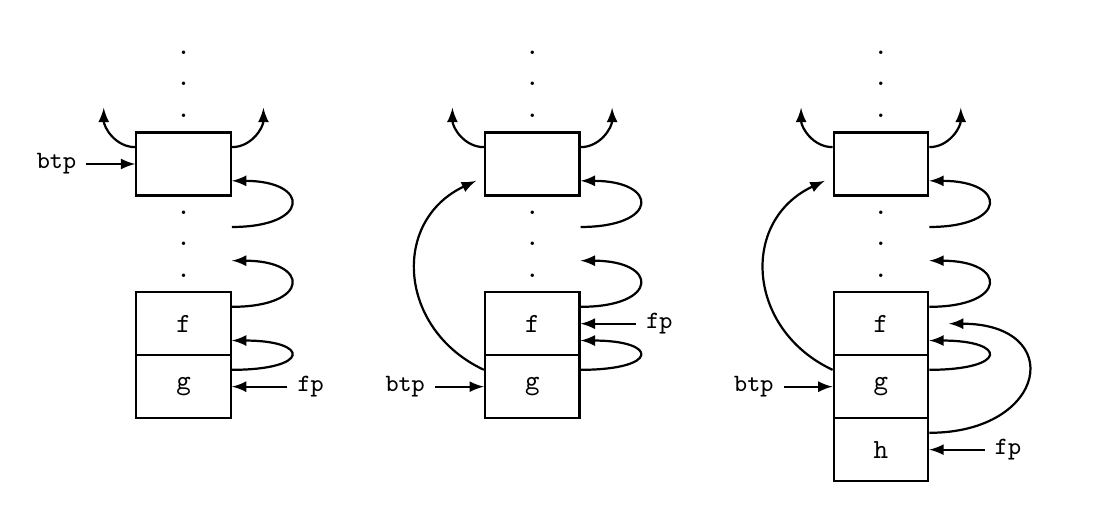
\begin{tikzpicture}[>=latex]
\matrix [thick, nodes={minimum height=4mm, minimum width=12mm, font=\tt}]
{
% uppper dots
% The matrix column sep option appears to add an extra separation after the final column
% so we use the first row to define the column separations
\node{.}; &[3.2cm] \node{.}; &[3.2cm] \node{.}; \\
\node{.}; & \node{.}; & \node{.}; \\
\node{.}; & \node{.}; & \node{.}; \\

% top row of empty boxes (tl = top left, tm = top middle, tr = top right)
\node (tl) [draw, minimum height=8mm] {}; &
\node (tm) [draw, minimum height=8mm] {}; &
\node (tr) [draw, minimum height=8mm] {};\\

% middle dots
\node{.}; & \node{.}; & \node{.}; \\
\node (mdl) {.}; & \node (mdm) {.}; & \node (mdr) {.}; \\ % mdl = middle dot left etc.
\node{.}; & \node{.}; & \node{.}; \\

% f boxes (left middle and right)
\node (fl) [draw, minimum height=8mm] {f}; & 
\node (fm) [draw, minimum height=8mm] {f}; &
\node (fr) [draw, minimum height=8mm] {f};\\[-0.8pt] % subtract width of a thick line to avoid a very thick line between boxes

% g boxes (left middle and right)
\node (gl) [draw, minimum height=8mm] {g}; &
\node (gm) [draw, minimum height=8mm] {g}; &
\node (gr) [draw, minimum height=8mm] {g}; &\\[-0.8pt]

 % h box (right only)
 & & \node (hr) [draw, minimum height=8mm] {h}; \\
};

% draw connecting arrows between the labelled nodes
\begin{scope}[thick,font=\tt\small]
\foreach \s / \d in {gm/tm, gr/tr} { % draw backtracking chain on the left
   \draw[->] ($(\s.north west) -(0,2mm)$) to [distance=1.2cm, out=155, in=205] ($(\d.south west) +(-1mm,2mm)$);
}
\foreach \s / \d in {gl/fl, gm/fm, gr/fr} { % connect g boxes to f boxes on the right
   \draw[->] ($(\s.north east) -(0,2mm)$) to [distance=1cm, out=0, in=0] ($(\d.south east)+ (0,2mm)$);
}
\foreach \s / \d in {mdl/tl, mdm/tm, mdr/tr} { % connect middle dots and top boxes
   \draw[->] (\s.north east) to [distance=1cm, out=0, in=0] ($(\d.south east)+ (0,2mm)$);
}
\foreach \s / \d in {fl/mdl, fm/mdm, fr/mdr} { %connect f boxes and middle dots
   \draw[->] ($(\s.north east) -(0,2mm)$) to [distance=1cm, out=0, in=0] (\d.south east);
}
\foreach \n in {tl, gm, gr} { % add btp pointers
  \draw ($(\n.west) - (1cm,0)$) node (x) {btp} ;
  \draw[->] (x.east) -- (\n.west);
}
\foreach \n in {gl, fm, hr} { % add fp pointers
  \draw ($(\n.east) + (1cm,0)$) node (x) {fp} ;
  \draw[->] (x.west) -- (\n.east);
}
\foreach \n in {tl,tm,tr} { % add left and right back pointers to top boxes
  \draw[->] ($(\n.north west) - (0,2mm)$) to [out=180, in=270] +(-0.4cm,0.5cm);
  \draw[->] ($(\n.north east) - (0,2mm)$) to [out=0, in=270] +(0.4cm,0.5cm);
}
\draw[->] ($(hr.north east) - (0,2mm)$) to [distance=1.5cm, out=0, in=0] ($(fr.east) + (0.25cm,0)$);
\end{scope}
%\draw[red] (current bounding box.south west) rectangle (current bounding box.north east);
\end{tikzpicture}

\par}

Suppose \texttt{g} produces the first of several possible
results. Execution returns to \texttt{f} and \texttt{g}'s frame is
added to the backtracking chain. This is represented by the middle
stack in the diagram. If \texttt{f} then calls \texttt{h}, its
procedure frame is added to the top of the stack as shown in the right
stack in the diagram.

If \texttt{h} produces a result and is not capable of producing more,
execution returns to \texttt{f} and the stack again looks like the one
in the middle of the diagram (the program pointer within \texttt{f} is
different, of course). If \texttt{h} produces a result and is capable
of producing more, execution returns to \texttt{f}, but \texttt{h}'s
frame remains on the stack and is added to the head backtracking
chain, similar to what was done when \texttt{g} produced a result.
If \texttt{h} produces no results, backtracking occurs.  \texttt{h}'s
frame is removed from the stack, execution returns to the
procedure \texttt{g} who's frame is at the head of the backtracking
chain, and \texttt{g}'s frame is removed from the head of the
chain. The stack once again looks like left stack in the diagram
and \texttt{g} proceeds to produce another result.


Traditional languages such as Pascal or C present high-level virtual
machines that contain no notion of backtracking and have no need to
perform low-level stack manipulations. Icon expressions with
goal-directed evaluation cannot be translated directly into such
languages. This is the fundamental problem that must be addressed when
designing a compiler for Icon. O'Bagy presents an elegant solution to
this problem in her dissertation [.tr88-31.]. Her solution is used by
this optimizing compiler as a basis for translating Icon expressions
into C code. The rest of this section contains a brief explanation of
the variation of her approach that is used in the compiler, while
exploring useful ways of viewing the problem. O'Bagy's dissertation
describes how control structures not covered in this discussion can be
implemented using her model.

Formal semantics is one tool that can be used in understanding a
language [.gordon denote,stoy.]. The added complexity caused by Icon's
goal-directed evaluation is reflected in Gudeman's description of Icon
using denotational semantics [.gudeman denotational.]. While
conventional programming languages can be described using one
continuation for each expression, Icon requires two continuations. One
continuation for an expression embodies the rest of the program if the
expression succeeds, while the other embodies the rest of the program
if the expression fails.

The Icon compiler uses the notion of success continuations to
implement goal-directed evaluation. However, these continuations
violate some of the properties traditionally associated with
continuations. A continuation in denotational semantics and in the
language Scheme [.Abelson,[Rees 86].] is a function that never
returns. However, the success continuations produced by the compiler
implement backtracking by returning. In addition, these continuations
implement the rest of the current bounded expression rather than the
rest of the entire program. Note that unlike continuations in Scheme,
these continuations are created at compile time, not at run time. Some
Prolog compilers have been based on a similar continuation-passing
technique [.Nilsson,Ramakrishnan.].

The C language is oriented toward an imperative style of
programming. In order to produce efficient code, the Icon compiler
should not generate an excessive number of function
calls. Specifically, it should avoid creating continuations for every
expression. A more operational view of Icon's semantics and of C's
semantics can be useful in understanding how to accomplish this. An
operation in Icon can succeed or fail. In the view of denotational
semantics, the question of what will be done in each case must be
answered, with the answers taking the form of functions. In an
operational view, the questions can take the form of where to go in
each case. The answers to these questions can be any type of transfer
of control supported by the C language: execute the next sequential
instruction, execute a function, return from a function, or go to a
label.

Most operations in Icon are \textit{monogenic}. That is, they produce
exactly one result, like operations in conventional languages. For
these operations, the compiler can generate code whose execution
simply falls through into the code that implements the subsequent
operation.

\textit{Conditional} operations are more interesting. These operations
either produce a single value or fail. If such an operation succeeds,
execution can fall through into code implementing the subsequent
operation. However, if the operation fails, execution must transfer
elsewhere in the program. This is accomplished by branching to a
\textit{failure label}. If the code for the operation is put in-line,
this is straightforward. However, if the operation (either a built-in
operation or an Icon procedure) is implemented by a separate C
function, the function must notify the caller whether it succeeded or
failed and the caller must effect the appropriate transfer of control.

By convention, C functions produced by the compiler and those
implementing the run-time routines each return a signal (this
convention is violated in some special cases). A signal is an integer
(and is unrelated to Unix signals). If one of these C functions needs
to return an Icon value, it does so through a pointer to a result
location that is passed to it as an argument. Two standard signals are
represented by the manifest constants \texttt{A\_Continue} and
\texttt{A\_Resume}. A return (either an Icon return expression or
the equivalent construct in a built-in operation) is implemented with
code similar to

\goodbreak
\begin{iconcode}
*result = \textit{operation result};\\
return A\_Continue;\\
\end{iconcode}

\noindent Failure is implemented with the code 

\iconline{return A\_Resume; }


\noindent The code implementing the call of an operation consists of
both a C call and signal-handling code.

\goodbreak
\begin{iconcode}
switch (\textit{operation}(\textit{args}, \&result)) \{\\
\>case A\_Continue: break;\\
\>case A\_Resume: goto failure label;\\
\}\\
\end{iconcode}


This code clearly can be simplified. This form is general enough to
handle the more complex signal handling that can arise during code
generation. Simplifying signal handling code is described in Chapter
21.


Generators pose the real challenge in implementing Icon. A generator
includes code that must be executed if subsequent failure occurs. In
addition, a generator, in general, needs to retain state information
between suspending and being resumed. As mentioned above, this is
accomplished by calling a success continuation. The success
continuation contains subsequent operations. If an operation in the
continuation fails, an \texttt{A\_Resume} signal is returned to the generator,
which then executes the appropriate code. The generator retains state
information in local variables. If the generator is implemented as a C
function, a pointer to the continuation is passed to it. Therefore, a
function implementing a generative operation need not know its success
continuation until run time.


Consider the operation \texttt{i to j}. This operation can be
implemented in Icon with a procedure like

\goodbreak
\begin{iconcode}
procedure To(i, j)\\
\>while i <= j do \{\\
\>\>suspend i\\
\>\>i +:= 1\\
\>\}\\
\>fail\\
end\\
\end{iconcode}


It can be implemented by an analogous C function similar to the
following (for simplicity, C ints are used here instead of Icon
values).

\goodbreak
\begin{iconcode}
int to(i, j, result, succ\_cont)\\
\>int i, j;\\
\>int *result;\\
\>int (*succ\_cont)();\\
\{\\
\>int signal;\\
\\
\>while (i <= j) \{\\
\>\>*result = i;\\
\>\>signal = (*succ\_cont)();\\
\>\>if (signal != A\_Resume)\\
\>\>\>return signal;\\
\>\>++i;\\
\>\}\\
\>return A\_Resume;\\
\}\\
\end{iconcode}

\noindent
There is no explicit failure label in this code, but it is possible to
view the code as if an implicit failure label occurs before the \texttt{++i}.


The Icon expression 

\iconline{every write(1 to 3) }

\noindent can be compiled into the following code (for simplicity, the
\texttt{write} function has been translated into \texttt{printf} and
scoping issues for result have been ignored). Note that the \texttt{every}
simply introduces failure.

\goodbreak
\begin{iconcode}
switch (to(1, 3, \&result, sc)) \{ /* standard signal-handling code */\\
\>\textit{...}\\
\}\\
\\
int sc() \{\\
\>printf("\%d{\textbackslash}n", result);\\
\>return A\_Resume;\\
\}\\
\end{iconcode}


The final aspect of Icon expression evaluation that must be dealt with
is that of bounded expressions. Once execution leaves a bounded
expression, that expression cannot be resumed. At this point, the
state of the computation with respect to backtracking looks as it did
when execution entered the bounded expression. This means that, in
generated code, where to go on failure (either by branching to an
explicit failure label or by returning an \texttt{A\_Resume} signal)
must be the same. However, this failure action is only correct in the
C function containing the start of the code for the bounded
expression. If a function suspended by calling a success continuation,
execution is no longer in that original C function. To accommodate
this restoration of failure action, execution must return to that
original function.

This is accomplished by setting up a \textit{bounding label} in the
original C function and allocating a signal that corresponds to the
label. When the end of the bounded expression is reached, the signal
for the bounding label is returned. When the signal reaches the
function containing the label, it is converted into
a \texttt{goto}. It can be determined statically which calls must
convert which signals. Note that if the bounded expression ends in the
original C function, the ``return signal'' is already in the context
of the label. In this case, it is immediately transformed into
a \texttt{goto} by the compiler, and there is no real signal handling.


Consider the Icon expression 

\goodbreak
\begin{iconcode}
move(1);\\
\>\textit{...}\\
\end{iconcode}

\noindent
The \texttt{move} function suspends and the C function implementing it
needs a success continuation. In this case, \texttt{move} is called in
a bounded context, so the success continuation must return execution
to the function that called \texttt{move}. The continuation makes use
of the fact that, like the C function for \texttt{to}, the one
for \texttt{move} only intercepts \texttt{A\_Resume} signals and
passes all other signals on to its caller.

This expression can be implemented with code similar to the
following. There are two possible signals that might be returned.
\texttt{move} itself might produce an \texttt{A\_Resume} signal or it
might pass along the bounding signal from the success continuation.
Note that for a compound expression, both the bounding label and the
failure label are the same. In general, this is not true. In this
context, the result of \texttt{move(1)} is discarded. The variable
\texttt{trashcan} receives this value; it is never read.

\goodbreak
\begin{iconcode}
\>switch (move(1, \&trashcan, sc)) \{\\
\>\>case 1:\\
\>\>\>goto L1;\\
\>\>case A\_Resume:\\
\>\>\>goto L1;\\
\>\}\\
L1: /* bounding label \& failure label */\\
\>\textit{...}\\
\end{iconcode}
\goodbreak
\begin{iconcode}
int sc() \{\\
\>return 1; /* bound signal */\\
\}\\
\end{iconcode}

\noindent
{\sffamily
Calling Conventions}


This discussion has touched on the subject of calling conventions for
run-time routines. In Icon, it is, in general, impossible to know
until run time what an invocation is invoking. This is handled in the
compiler with a standard calling convention for the C functions
implementing operations and procedures. This calling convention allows
a C function to be called without knowing anything about the operation
it implements.

A function conforming to the standard calling convention has four
parameters. These parameters are, in order of appearance, the number
of Icon arguments (a C int), a pointer to the beginning of an array of
descriptors holding the Icon arguments, a pointer to the descriptor
used as the Icon result location, and a success continuation to use
for suspension. The function itself is responsible for any argument
conversions including dereferencing, and for argument list
adjustment. As explained above, the function returns an integer
signal. The function is allowed to return the signals
\texttt{A\_Resume}, \texttt{A\_Continue}, and any signals returned by
the success continuation. It may ignore the success continuation if it
does not suspend. The function may be passed a null continuation. This
indicates that the function will not be resumed. In this case, suspend
acts like a simple return, passing back the signal \texttt{A\_Continue}
(this is not shown in the examples). The outline of a
standard-conforming function is

\goodbreak
\begin{iconcode}
int \textit{function-name}(nargs, args, result, succ\_cont)\\
int nargs; dptr args; dptr result;\\
continuation succ\_cont;\\
\{\\
\>\ ...\\
\}\\
\end{iconcode}

\noindent
\texttt{continuation} is defined to be a pointer to a function taking
no arguments and returning an integer.

Later sections of this dissertation describe the code generation
process in more detail and describe optimizations of various parts of
the code including parameter passing, continuations, signal handling,
and branching.


\bigskip

\clearpage
\bigskip

\clearpage\chapter{The Type Inferencing Model}

Three sections of this dissertation are devoted to type inferencing:
two chapters and an appendix. This chapter develops a theoretical
model of type inferencing for Icon. For simplicity, it ignores some
features of the language. This chapter presents intuitive arguments
for the correctness of the formal model. Chapter 19 describes the
actual implementation of type inferencing in the Icon compiler. The
implementation handles the full Icon language and, for pragmatic
reasons, differs from the theoretical model in some details.


This chapter starts with the motivation for performing type
inferencing. It then describes the concept of \textit{abstract
interpretation}. This concept is used as a tool in this chapter to
develop a type inferencing system from Icon's semantics. This chapter
gives an intuitive presentation of this development process before
presenting the formal models of abstract semantics for Icon. The most
abstract of the formal models is the type inferencing system.

\section[15.1 Motivation]{15.1 Motivation}

Variables in the Icon programming language are untyped. That is, a
variable may take on values of different types as the execution of a
program proceeds. In the following example, \texttt{x} contains a
string after the read (if the read succeeds), but it is then assigned
an integer or real, provided the string can be converted to a numeric
type.

\goodbreak
\begin{iconcode}
x := read()\\
if numeric(x) then x +:= 4\\
\end{iconcode}


In general, it is impossible to know the type of an operator's
operands at translation time, so some type checking must be done at
run time. This type checking may result in type conversions, run-time
errors, or the selection among polymorphous operations (for example,
the selection of integer versus real addition). In the Icon
interpreter system, all operators check all of their operands at run
time. This incurs significant overhead.

Much of this run-time type checking is unnecessary. An examination of
typical Icon programs reveals that the types of most variables remain
consistent throughout execution (except for the initial null value)
and that these types can often be determined by inspection. Consider

\goodbreak
\begin{iconcode}
if x := read() then\\
\>y := x || ";"\\
\end{iconcode}


Clearly both operands of {\textbar}{\textbar} are strings so no
checking or conversion is needed.

The goal of a type inferencing system is to determine what types
variables may take on during the execution of a program. It associates
with each variable usage a set of the possible types of values that
variable might have when execution reaches the usage. This set may be
a conservative estimate (overestimate) of the actual set of possible
types that a variable may take on because the actual set may not be
computable, or because an analysis to compute the actual set may be
too expensive. However, a good type inferencing system operating on
realistic programs can determine the exact set of types for most
operands and the majority of these sets in fact contain single types,
which is the information needed to generate code without type
checking. The Icon compiler has an effective type inferencing system
based on data flow analysis techniques.

\section[15.2 Abstract Interpretation ]{15.2 Abstract Interpretation }

Data flow analysis can be viewed as a form of abstract interpretation
[.absintrp.]. This can be particularly useful for understanding type
inferencing. A ``concrete'' interpreter for a language implements the
standard (operational) semantics of the language, producing a sequence
of states, where a state consists of an execution point, bindings of
program variables to values, and so forth. An abstract interpreter
does not implement the semantics, but rather computes information
related to the semantics. For example, an abstract interpretation may
compute the sign of an arithmetic expression rather than its
value. Often it computes a ``conservative'' estimate for the property
of interest rather than computing exact information. Data flow
analysis is simply a form of abstract interpretation that is
guaranteed to terminate. This chapter presents a sequence of
approximations to Icon semantics, culminating in one suitable for type
inferencing.

Consider a simplified operational semantics for Icon, consisting only
of program points (with the current execution point maintained in a
program counter) and variable bindings (maintained in an
environment). As an example of these semantics, consider the following
program. Four program points are annotated with numbers using comments
(there are numerous intermediate points not annotated).

\goodbreak
\begin{iconcode}
procedure main()\\
local s, n\\
\\
\>\# 1:\\
\>s := read()\\
\>\# 2:\\
\>every n := 1 to 2 do \{\\
\>\>\# 3:\\
\>\>write(s[n])\\
\>\>\}\\
\>\# 4:\\
end\\
\end{iconcode}


If the program is executed with an input of \texttt{abc}, the following states
are included in the execution sequence (only the annotated points are
listed). States are expressed in the form \textit{program point}:
\textit{environment}.

\goodbreak
\begin{specialcode}{}
\>\>1: [\texttt{s} = null, \texttt{n} = null]\\
\>\>2: [\texttt{s} = "\texttt{abc}", \texttt{n} = null]\\
\>\>3: [\texttt{s} = "\texttt{abc}", \texttt{n} = 1]\\
\>\>3: [\texttt{s} = "\texttt{abc}", \texttt{n} = 2]\\
\>\>4: [\texttt{s} = "\texttt{abc}", \texttt{n} = 2]\\
\end{specialcode}


It is customary to use the \textit{collecting semantics} of a language
as the first abstraction (approximation) to the standard semantics of
the language. The collecting semantics of a program is defined in
Cousot and Cousot [.absintrp.]  (they use the term \textit{static
semantics}) to be an association between program points and the sets
of environments that can occur at those points during all possible
executions of the program.

Once again, consider the previous example. In general, the input to
the program is unknown, so the read function is assumed to be capable
of producing any string. Representing this general case, the set of
environments (once again showing only variable bindings) that can
occur at point 3 is

\goodbreak
\begin{specialcode}{}
\>\>[\texttt{s} = "", \texttt{n} = 1],\\
\>\>[\texttt{s} = "", \texttt{n} = 2],\\
\>\>[\texttt{s} = "a", \texttt{n} = 1],\\
\>\>[\texttt{s} = "a", \texttt{n} = 2],\\
\>\>\>\ \ldots\\
\>\>[\texttt{s} = "\texttt{abcd}", \texttt{n} = 1],\\
\>\>[\texttt{s} = "\texttt{abcd}", \texttt{n} = 2],\\
\>\>\> \ldots\\
\end{specialcode}


A type inferencing abstraction further approximates this information,
producing an association between each variable and a type at each
program point. The actual type system chosen for this abstraction must
be based on the language and the use to which the information is
put. The type system used here is based on Icon's run-time type
system. For structure types, the system used retains more information
than a simple use of Icon's type system would retain; this is
explained in detail later. For atomic types, Icon's type system is
used as is. For point 3 in the preceding example the associations
between variables and types are

\begin{specialcode}{}
\>\>[\texttt{s} = string, \texttt{n} = integer]\\
\end{specialcode}

The type inferencing system presented in this chapter is best
understood as the culmination of a sequence of abstractions to the
semantics of Icon, where each abstraction discards certain
information. For example, the collecting semantics discards sequencing
information among states; in the preceding program, collecting
semantics determine that, at point 3, states may occur with \texttt{n}
equal to 1 and with \texttt{n} equal to 2, but does not determine the
order in which they must occur. This sequencing information is
discarded because desired type information is a static property of the
program.


The first abstraction beyond the collecting semantics discards dynamic
control flow information for goal directed evaluation. The second
abstraction collects, for each variable, the value associated with the
variable in each environment. It discards information such as,
``\texttt{x} has the value 3 when \texttt{y} has the value 7'',
replacing it with ``\texttt{x} may have the value 3 sometime
and \texttt{y} may have the value 7 sometime.''. It effectively
decouples associations between variables.

This second abstraction associates a set of values with a variable,
but this set may be any of an infinite number of sets and it may
contain an infinite number of values. In general, this precludes
either a finite computation of the sets or a finite representation of
them. The third abstraction defines a type system that has a finite
representation.  This abstraction discards information by increasing
the set associated with a variable (that is, making the set less
precise) until it matches a type. This third model can be implemented
with standard iterative data flow analysis techniques.

This chapter assumes that an Icon program consists of a single
procedure and that all invocations are to built-in functions. It also
assumes that there are no co-expressions beyond the main
co-expression. See Chapter 19 for information on how to extend the
abstractions to multiple procedures and multiple co-expressions.


\section[15.3 Collecting Semantics]{15.3 Collecting Semantics}

The collecting semantics of an Icon program is defined in terms of a
\textit{flow graph} of the program. A flow graph is a directed graph
used to represent the flow of control in a program. Nodes in the graph
represent the executable primitives in the program. An edge exists
from node \textbf{A} to node \textbf{B} if it is possible for
execution to pass directly from the primitive represented by node
\textbf{A} to the primitive represented by node \textbf{B}. Cousot and
Cousot [.absintrp.] prove that the collecting semantics of a program
can be represented as the least fixed point of a set of equations
defined over the edges of the program's flow graph. These equations
operate on sets of environments.

For an example of a flow graph, consider the Icon program 

\goodbreak
\begin{iconcode}
procedure main()\\
\>every write(1 to 3)\\
end\\
\end{iconcode}

\noindent
The diagram below on the left shows the abstract syntax tree for this
procedure, including the implicit \texttt{fail} at the end of the
procedure. The invoke node in the syntax tree represents procedure
invocation. Its first argument must evaluate to the procedure to be
invoked; in this case the first argument is the global variable
\texttt{write}. The rest of the arguments are used as the arguments to the
procedure. \texttt{pfail} represents procedure failure (as opposed to
expression failure within a procedure). Nodes corresponding to
operations that produce values are numbered for purposes explained
below.

A flow graph can be derived from the syntax tree. This is shown on the right. 

\begin{picture}(400,250)
%\put(0,0){\graphpaper{40}{25}}
\put(0,0){\includegraphics[width=2.4in,height=3.4in]{kw/figure3-1.png}}
\put(200,20){\includegraphics[width=2.2in,height=3.1in]{kw/figure3-2.png}}
\end{picture}

The node labeled procedure main is the \textit{start node} for the
procedure; it performs any necessary initializations to establish the
execution environment for the procedure. The edge from \texttt{invoke}
to \texttt{to} is a resumption path induced by the control structure
\texttt{every}. The path from \texttt{to} to \texttt{pfail} is the
failure path for \texttt{to}. It is a forward execution path rather
than a resumption path because the compound expression (indicated by
\texttt{;}) limits backtracking out of its left-hand sub-expression.
Chapter 19 describes how to determine the edges of the flow graph for
an Icon program.

Both the standard semantics and the abstract semantics must deal with
the intermediate results of expression evaluation.  A
temporary-variable model is used because it is more convenient for
this analysis than a stack model. This decision is unrelated to the
use of a temporary-variable model in the compiler. This analysis uses
a trivial assignment of temporary variables to intermediate
results. Temporary variables are not reused. Each node that produces a
result is assigned some temporary variable \textit{ri} in the
environment. Assuming that temporary variables are assigned to the
example according to the node numbering, the \texttt{to} operation has
the effect of

\iconline{\>\>\ttit{r3} := \ttit{r4} to \ttit{r5} }

\noindent
Expressions that represent alternate computations must be assigned the
same temporary variable, as in the following example for the
subexpression \texttt{x := ("a" {\textbar} "b")}. The syntax tree
below on the left and the flow graph are shown on the right.

\begin{picture}(400,180)
%\put(0,0){\graphpaper{40}{18}}
\put(0,0){\includegraphics[width=2.2492in,height=2.2398in]{kw/figure3-3.png}}
\put(200,0){\includegraphics[width=2.4154in,height=2.3in]{kw/figure3-4.png}}
\end{picture}

The \texttt{if} and \texttt{case} control structures are handled
similarly. In addition to temporary variables for intermediate
results, some generators may need additional temporary variables to
hold internal states during suspension. It is easy to devise a scheme
to allocate them where they are needed; details are not presented
here. The syntax tree is kept during abstract interpretation and used
to determine the temporary variables associated with an operation and
its operands.

The equations that determine the collecting semantics of the program
are derived directly from the standard semantics of the language. The
set of environments on an edge of the flow graph is related to the
sets of environments on edges coming into the node at the head of this
edge. This relationship is derived by applying the meaning of the node
(in the standard semantics) to each of the incoming environments.

It requires a rather complex environment to capture the full
operational semantics (and collecting semantics) of a language like
Icon. For example, the environment needs to include a representation
of the external file system.  However, later abstractions only use the
fact that the function \texttt{read} produces strings. This discussion
assumes that it is possible to represent the file system in the
environment, but does not give a representation. Other complexities of
the environment are discussed later. For the moment, examples only
show the bindings of variables to unstructured (atomic) values.

As an example of environments associated with the edges of a flow
graph, consider the assignment at the end of the following code
fragment. The comments in the if expression are assertions that are
assumed to hold at those points in the example.

\goodbreak
\begin{iconcode}
\>if x = 7 then \{\\
\>\>...\\
\>\>\# x is 7 and y is 3\\
\>\>\}\\
\>else \{\\
\>\>...\\
\>\>\# (x is null and y is 1) or (x is "abc" and y is 2)\\
\>\>\}\\
\>x := y + 2\\
\end{iconcode}


Because of the preceding \texttt{if} expression, there are two paths
reaching the assignment. The diagram below shows the flow graph and
accompanying environments for the expression; the diagram ignores the
fact that the assignment expression requires several primitive
operations to implement.


 \includegraphics[width=6.0in,height=2.1in]{kw/figure3-5.png}  


For a conditional expression, an incoming environment is propagated to
the path that it would cause execution to take in the standard
semantics. This requires distinguishing the paths to be taken on
failure (backtracking paths) from those to be taken on success. The
following diagram shows an example of this.

{\centering  \includegraphics[width=5.3992in,height=2.2299in]{kw/figure3-6.png} \par}

In general there may be several possible backtracking paths. The
environments in the standard and collecting semantics need to include
a stack of current backtracking points and control flow information,
and the flow graph needs instructions to maintain this stack. The Icon
interpreter system described in Part I is an example of how this
information can be maintained. However, the first abstraction to the
collecting semantics eliminates the need for this information, so the
information is not presented in detail here.

\section{Model 1: Eliminating Control Flow Information}

The first abstraction involves taking the union of the environments
propagated along all the failure paths from a node in the collecting
semantics and propagating that union along each of the failure paths
in the new abstraction. This abstraction eliminates the stack of
backtracking points from the environment.

A more formal definition for this model requires taking a closer look
at Icon data values, especially those values with internal
structure. In order to handle Icon data objects with pointer
semantics, an environment needs more than variable bindings. This fact
is important to type inferencing. The problem is handled by including
two components in the environment. The first is the \textit{store},
which maps variables to values. Variables include \textit{named}
variables, \textit{temporary} variables, and \textit{structure}
variables. Named variables correspond to program
identifiers. Temporary variables hold intermediate results as
discussed above. Structure variables are elements of structures such
as lists. Note that the sets of named variables and temporary
variables are each finite (based on the assumption that a program
consists of a single non-recursive procedure; as mentioned earlier,
this assumption is removed in Chapter 19), but for some
non-terminating programs, the set of structure variables may be
infinite.  \textit{Program} variables include both named variables and
structure variables but not temporary variables.

Values include atomic data values such as integers, csets, and
strings. They also include \textit{pointers} that reference objects
with pointer semantics. In addition to the values just described,
temporary variables may contain references to program variables. These
\textit{variable references} may be used by assignments to update the
store or they may be dereferenced by other operations to obtain the
values stored in the variables.

The second part of the environment is the \textit{heap}. It maps
pointers to the corresponding data objects (this differs from the heap
in the Icon implementation in that that heap also contains some data
objects that do not have pointer semantics). For simplicity, the only
data type with pointer semantics included in this discussion is the
list.  A list is a partial mapping from integers to
variables. Representing other data types with pointer semantics is
straightforward; this is discussed in Chapter 19.

The first abstraction is called Model 1. The notations envir$_{[n]}$,
store$_{[n]}$, and heap$_{[n]}$ refer to the sets of possible
environments, stores, and heaps respectively in model $n$. For
example, envir$_{[1]}$ is the set of possible environments in the
first abstraction. In the following set of definitions, $X \times Y$
is the set of ordered pairs where the first value in the pair is from
$X$ and the second value is from $Y$. $ X \rightarrow Y$ is the set of
partial functions from $X$ to $Y$. The definition of the set of
possible environments for model 1 is

\goodbreak
\begin{specialcode}{}
\>envir$_{[1]}$ = store$_{[1]}$ $\times$ heap$_{[1]}$\\
\>store$_{[1]}$ = variables $\rightarrow$ values\\
\>values       = integers $\cup$ strings $\cup$ \ldots $\cup$ pointers $\cup$ variables\\
\>heap$_{[1]}$  = pointers \textrm{${\rightarrow}$} lists,~%
                 where lists = integers $\rightarrow$ variables\\
\end{specialcode}


For example, the expression 

\iconline{ \>a := ["abc"] }

\noindent creates a list of one element whose value is the string \texttt{abc}
and assigns the list to the variable \texttt{a}. Let $p_1$ be the
pointer to the list and let $v_1$ be the (anonymous) variable within
the list. The resulting environment, e $\in$ envir$_{[1]}$, might be

\goodbreak
\begin{specialcode}{}
\>e = $(s,h)$, where $s \in $ store$_{[1]}$, $h \in $ heap$_{[1]}$\\
\>$s($\texttt{a}$) = p_1$\\
\>$s(v_1) = $ "\texttt{abc}"\\
\\
\>$h(p_1) = L_1$, where $L_1 \in$ lists\\
\\
\>$L_1(1) = v_1$\\
\end{specialcode}

\noindent
If the statement 

\iconline{ \>a[1] := "xyz" }


\noindent is executed, the subscripting operation dereferences \texttt{a}
producing $p_1$, then uses the heap to find $L_1$, which it applies to
1 to produce the result $v_1$. The only change in the environment at
this point is to temporary variables that are not shown. The
assignment then updates the store, producing

\goodbreak
\begin{iconcode}
\>$e_1 = (s_1 , h)$\\
\>$s_1$(\texttt{a})$ = p_1$\\
\>$s_1(v_1) =$ "xyz"\\
\end{iconcode}

\noindent
Assignment does not change the heap. On the other hand, the expression 

\iconline{ \ \ put(a, "xyz") }

\noindent adds the string \texttt{xyz} to the end of the list; if it is
executed in the environment $e$, it alters the heap along with adding a
new variable to the store.

\goodbreak
\begin{specialcode}{}
\>$e_1 = (s_1 , h_1$)\\
\>$s_1($\texttt{a}$) = p_1$\\
\>$s_1(v_1) =$ "\texttt{abc}"\\
\>$s_1(v_2) =$ "\texttt{xyz}"\\
\>$h_1(p_1) = L_2$\\
\>$L_2(1) = v_1$\\
\>$L_2(2) = v_2$\\
\end{specialcode}


If a formal model were developed for the collecting semantics, it
would have an environment similar to the one in Model 1. However, it
would need a third component with which to represent the backtracking
stack.

\section{Model 2: Decoupling Variables}

The next approximation to Icon semantics, Model 2, takes all the
values that a variable might have at a given program point and gathers
them together. In general, a variable may have the same value in many
environments, so this, in some sense, reduces the amount of space
required to store the information (though the space may still be
unbounded). The ``cost'' of this reduction of storage is that any
information about relationship of values between variables is lost.

Model 2 is also defined in terms of environments, stores, and heaps,
although they are different from those of Model 1.  A store in Model 2
maps sets of variables to sets of values; each resulting set contains
the values associated with the corresponding variables in environments
in Model 1. Similarly, a heap in Model 2 maps sets of pointers to sets
of lists; each of these sets contains the lists associated with the
corresponding pointers in environments in Model 1. An environment in
Model 2 contains a store and a heap, but unlike in Model 1, there is
only one of these environments associated with each program point. The
environment is constructed so that it effectively ``contains'' the
environments in the set associated with the point in Model 1.

The definition of Model 2 is 


\goodbreak
\begin{specialcode}{}
\>envir$_{[2]}$  =  store$_{[2]} \times $ heap$_{[2]}$\\
\>store$_{[2]}$  =  $2^{\textrm{variables}} \rightarrow 2^{\textrm{values}}$ \\
\>heap$_{[2]}$   =  $2^{\textrm{pointers}} \rightarrow 2^{\textrm{lists}}$ \\
\end{specialcode}

In Model 1, operations produce elements from the set
\textit{values}. In Model 2, operations produce subsets of this
set. It is in this model that \texttt{read} is taken to produce the
set of all strings and that the existence of an external file system
can be ignored.

Suppose a program point is annotated with the set containing the
following two environments from Model 1.

\goodbreak
\begin{iconcode}
\> $e_1,e_2 \in$ envir$_{[1]}$\\
\> $e_1 = (s_1, h_1)$\\
\> $s_1($\texttt{x}$) = 1$\\
\> $s_1($\texttt{y}$) = p_1$\\
\> $h_1(p_1) = L_1$\\
\\
\> $e_2 = (s_2, h_2)$\\
\> $s_2($\texttt{x}$) = 2$\\
\> $s_2($\texttt{y}$) = p_1$\\
\> $h_2(p_1) = L_2$\\
\end{iconcode}

\noindent
Under Model 2 the program point is annotated with the single
environment $\hat{e} {\in}$ envir$_{[2]}$, where

\goodbreak
\begin{iconcode}
\> $\hat{e} = (\hat{s},\hat{h})$\\
\> $\hat{s}(\{$\texttt{x}\}$) = \{1,2\}$\\
\> $\hat{s}(\{$\texttt{y}\}$) = \{p_1\}$\\
\> $\hat{s}(\{$\texttt{x}, \texttt{y}\}$) = \{1, 2, p_1\}$\\
\> $\hat{h}(\{p_1\}) = \{L_1, L_2\}$\\
\end{iconcode}

\noindent
Note that a store in Model 2 is distributive over union. That is, 


$\hat{s}(X \cup Y) = \hat{s}(X) \cup \hat{s}(Y)$

\noindent
so listing the result of $\hat{s}(\{$\texttt{x}, \texttt{y}$\})$ is
redundant. A heap in Model 2 also is distributive over union.

In going to Model 2 information is lost. In the last example, the fact
that \texttt{x = 1} is paired with $p_1 =L_1$ and \texttt{x = 2} is
paired with $p_1 = L_2$ is not represented in Model 2.

Just as \texttt{read} is extended to produce a set of values, so are
all other operations. These "extended" operations are then used to set
up the equations whose solution formally defines Model 2. This
extension is straightforward. For example, the result of applying a
unary operator to a set is the set obtained by applying the operator
to each of the elements in the operand. The result of applying a
binary operator to two sets is the set obtained by applying the
operator to all pairs of elements from the two operands. Operations
with more operands are treated similarly. For example

\begin{eqnarray*}
\{1, 3, 5\} + \{2, 4\} & = & \{1 + 2, 1 + 4, 3 + 2, 3 + 4, 5 + 2, 5 + 4\}\\
                       & = & \{3, 5, 5, 7, 7, 9\}\\
                       & = & \{3, 5, 7, 9\}\\
\end{eqnarray*}

The loss of information mentioned above affects the calculation of
environments in Model 2. Suppose the addition in the last example is
from

\iconline{\>z := x + y }

\noindent and that Model 1 has the following three environments at the
point before the calculation

\goodbreak
\begin{iconcode}
\>[x = 1, y = 2, z = 0]\\
\>[x = 3, y = 2, z = 0]\\
\>[x = 5, y = 4, z = 0]\\
\end{iconcode}


After the calculation the three environments will be 

\goodbreak
\begin{iconcode}
\>[x = 1, y = 2, z = 3]\\
\>[x = 3, y = 2, z = 5]\\
\>[x = 5, y = 4, z = 9]\\
\end{iconcode}

If these latter three environments are translated into an environment
of Model 2, the result is

\iconline{ \>[x = \{1, 3, 5\}, y = \{2, 4\}, z = \{3, 5, 9\}] }


However, when doing the computation using the semantics of + in Model
2, the value for \texttt{z} is \texttt{\{3, 5, 7, 9\}}. The solution
to the equations in Model 2 overestimates (that is, gives a
conservative estimate for) the values obtained by computing a solution
using Model 1 and translating it into the domain of Model 2.

Consider the following code with respect to the semantics of
assignment in Model 2. (Assume that the code is executed once, so only
one list is created.)

\goodbreak
\begin{iconcode}
\>x := [10, 20]\\
\>i := if read() then 1 else 2\\
\>x[i] := 30\\
\end{iconcode}

After the first two assignments, the store maps \texttt{x} to a set containing
one pointer and maps \texttt{i} to a set containing 1 and 2. The third
assignment is not as straightforward. Its left operand evaluates to
two variables; the most that can be said about one of these variables
after the assignment is that it might have been assigned 30. If $(s, h)$
is the environment after the third assignment then

\goodbreak
\begin{specialcode}{}
\>$s(\{$\texttt{x}$\}) = \{ p_1 \}$\\
\>$s(\{$\texttt{i}$\}) = \{1, 2\}$\\
\>$s(\{v_1\}) = \{10, 30\}$\\
\>$s(\{v_2\}) = \{20, 30\}$\\
\\
\>$h(\{p_1\}) = \{L_1\}$\\
\\
\>$L_1(1) = v_1$\\
\>$L_1(2) = v_2$\\
\end{specialcode}


Clearly all assignments could be treated as \textit{weak updates}
[.pntstr.], where a weak update is an update that may or may not take
place. However, this would involve discarding too much information;
assignments would only add to the values associated with variables and
not replace the values. Therefore assignments where the left hand side
evaluates to a set containing a single variable are treated as special
cases. These are implemented as \textit{strong updates}.

\section{Model 3: A Finite Type System}

The environments in Model 2 can contain infinite amounts of
information, as in the program

\goodbreak
\begin{iconcode}
\>x := 1\\
\>repeat x +:= 1\\
\end{iconcode}

\noindent where the set of values associated with x in the loop
consists of all the counting numbers. Because equations in Model 2 can
involve arbitrary arithmetic, no algorithm can find the least fixed
point of an arbitrary set of these equations.

The final step is to impose a finitely representable type system on
values. A type is a (possibly infinite) set of values. The type system
presented here includes three classifications of basic types. The
first classification consists of the Icon types without pointer
semantics: integers, strings, csets, etc. The second classification
groups pointers together according to the lexical point of their
creation. This is similar to the method used to handle recursive data
structures in Jones and Muchnick [.analrcsv.]. Consider the code

\iconline{ \>every insert(x, [1 to 5]) }


If this code is executed once, five lists are created, but they are
all created at the same point in the program, so they all belong to
the same type. The intuition behind this choice of types is that
structures created at the same point in a program are likely to have
components of the same type, while structures created at different
points in a program may have components of different types.

The third classification of basic types handles variable
references. Each named variable and temporary variable is given a type
to itself. Therefore, if \texttt{a} is a named variable,
\texttt{\{a\}} is a type. Structure variables are grouped into types
according to the program point where the pointer to the structure is
created. This is not necessarily the point where the variable is
created; in the following code, a pointer to a list is created at one
program point, but variables are added to the list at different points

\goodbreak
\begin{iconcode}
\ \ x := []\\
\ \ push(x, 1)\\
\ \ push(x ,2)\\
\end{iconcode}


References to these variables are grouped into a type associated with
the program point for \texttt{[]}, not the point for the corresponding
push.

If a program contains k non-structure variables and there are n
locations where pointers can be created, then the basic types for the
program are integer, string, ..., P\TextSubscript{1}, ...,
P\TextSubscript{n}, V\TextSubscript{1}, ..., V\TextSubscript{n},
\{v\TextSubscript{1}\}, ..., \{v\TextSubscript{k}\} where
P\TextSubscript{i} is the pointer type created at location i,
V\TextSubscript{i} is the variable type associated with
P\TextSubscript{i}, and v\TextSubscript{i} is a named variable or a
temporary variable. Because programs are lexically finite they each
have a finite number of basic types. The set of all types for a
program is the smallest set that is closed under union and contains
the empty set along with the basic types:

\begin{specialcode}{}
\>types = \{\{\}, integers, strings,...,~%
    (integers ${\cup}$ \ strings),...,~%
    (integers ${\cup}$ strings ${\cup}$ ... ${\cup}$ \{v\TextSubscript{k}\})\}
\end{specialcode}

Model 3 replaces the arbitrary sets of values of Model 2 by
types. This replacement reduces the precision of the information, but
allows for a finite representation and allows the information to be
computed in finite time.

In Model 3, both the store and the heap map types to types. This store
is referred to as the \textit{type store}. The domain of type store is
\textit{variable types}, that is, those types whose only values are
variable references.  Similarly, the domain of the heap is
\textit{pointer types}. Its range is the set types containing only
structure variables. A set of values from Model 2 is converted to a
type in Model 3 by mapping that set to the smallest type containing
it. For example, the set

\iconline{ \>\{1, 4, 5, "23", "0"\} }

\noindent is mapped to

\begin{specialcode}{}
\>integer ${\cup}$ string\\
\end{specialcode}

\noindent
The definition of envir$_{[3]}$ is 

\goodbreak
\begin{specialcode}{}
\>envir$_{[3]} = $ store$_{[3]} \times $ heap$_{[3]}$\\
\>store$_{[3]} = $ variable-types $\rightarrow $ types\\
\>heap$_{[3]} = $ pointer-types $\rightarrow $ structure-variable-types\\
\>types ${\subseteq}$ 2\textsuperscript{values}\\
\>variable-types ${\subseteq}$ types\\
\>structure-variable-types ${\subseteq}$ variable-types\\
\>pointer-types ${\subseteq}$ types\\
\end{specialcode}


There is exactly one variable type for each pointer type in this
model. The heap simply consists of this one-to-one mapping; the heap
is of the form

{\ttfamily\mdseries
\ \ \ $h$( P\TextSubscript{i} ) = V\TextSubscript{i}}

This mapping is invariant over a given program. Therefore, the type
equations for a program can be defined over store$_{[3]}$ rather than
envir$_{[3]}$ with the heap embedded within the type equations.

Suppose an environment from Model 2 is 

\goodbreak
\begin{specialcode}{}
\> $e \in $ envir$_{[2]}$\\
\> $e = (s, h)$\\
\\
\> $s(\{$\texttt{a}$\}) = \{ p_1 , p_2\}$\\
\> $s(\{v_1\}) = \{1, 2\}$\\
\> $s(\{v_2\}) = \{1\}$\\
\> $s(\{v_3\}) = \{12.03\}$\\
\\
\> $h(\{p_1\}) = \{L_1, L_2\}$\\
\> $h(\{p_2\}) = \{L_3\}$\\
\\
\> $L_1(1) = v_1$\\
\\
\> $L_2(1) = v_1$\\
\> $L_2(2) = v_2$\\
\\
\> $L_3(1) = v_3$\\
\end{specialcode}

Suppose the pointers p\TextSubscript{1} and p\TextSubscript{2} are
both created at program point 1. Then the associated pointer type is
P\TextSubscript{1} and the associated variable type is
V\TextSubscript{1}. The corresponding environment in Model 3 is

\goodbreak
\begin{specialcode}{}
\>$\hat{e} \in $ envir$_{[3]}$\\
\>$\hat{e} = (\hat{s},\hat{h})$\\

\>$\hat{s}(\{$\texttt{a}$\}) =  $ P$_1$\\
\>$\hat{s}($V$_1) = $ integer  $\cup$ real\\

\>$\hat{h}($P$_1) = $ V$_1$\\
\end{specialcode}



The collecting semantics of a program establishes a set of (possibly)
recursive equations between the sets of environments on the edges of
the program's flow graph. The collecting semantics of the program is
the least fixed point of these equations in which the set on the edge
entering the start state contains all possible initial environments.
Similarly, type inferencing establishes a set of recursive equations
between the type stores on the edges of the flow graph. The least
fixed point of these type inferencing equations is computable using
iterative methods. This is discussed in Chapter 19. The fact that
these equations have solutions is due to the fact that the equations
in the collecting semantics have a solution and the fact the each
abstraction maintains the ``structure'' of the problem, simply
discarding some details.

Chapter 19 also extends type inferencing to handle the entire Icon
language. Chapter 22 uses the information from type inferencing to
optimize the generated code.


\chapter{Liveness Analysis of Intermediate Values}

The maintenance of intermediate values during expression evaluation in
the Icon programming language is more complicated than it is for
conventional languages such as C and Pascal. O'Bagy explains this in
her dissertation [.tr88-31.]:

\begin{quote}
``Generators prolong the lifetime of temporary values. For example, in 

\iconline{\>\>i = find(s1,s2)}

\noindent
the operands of the comparison operation cannot be discarded when
\texttt{find} produces its result. If \texttt{find} is resumed, the
comparison is performed again with subsequent results from
\texttt{find(s1,s2}), and the left operand must still be available.''
\end{quote}

\noindent In some implementation models, it is equally important that
the operands of \texttt{find} still be available if that function is
resumed (this depends on whether the operand locations are used during
resumption or whether all needed values are saved in the local state
of the function).

As noted in Chapter 14, a stack-based model handles the lifetime
problem dynamically. However, a temporary-variable model like the one
used in this compiler requires knowledge at compile-time of the
lifetime of intermediate values. In a straightforward implementation
of conventional languages, liveness analysis of intermediate values is
trivial: an intermediate value is computed in one place in the
generated code, is used in one place, and is live in the contiguous
region between the computation and the use. In such languages,
determining the lifetime of intermediate values only becomes
complicated when certain optimizations are performed, such as code
motion and common subexpression elimination across basic blocks
[.dragonbk,progflw.]. This is not true in Icon. In the presence of
goal-directed evaluation, the lifetime of an intermediate value can
extend beyond the point of use. Even in a straightforward
implementation, liveness analysis is not trivial.

In its most general form, needed in the presence of the optimizations
mentioned above, liveness analysis requires iterative
methods. However, goal-directed evaluation imposes enough structure on
the liveness problem that, at least in the absence of optimizations,
iterative methods are not needed to solve it. This chapter presents a
simple and accurate method for computing liveness information for
intermediate values in Icon. The analysis is formalized in an
attribute grammar.


\section[16.1 Implicit Loops]{16.1 Implicit Loops}

Goal-directed evaluation extends the lifetime of intermediate values
by creating implicit loops within an expression. In O'Bagy's example,
the start of the loop is the generator \texttt{find} and the end of
the loop is the comparison that may fail.  An intermediate value may
be used within such a loop, but if its value is computed before the
loop is entered, it is not recomputed on each iteration and the
temporary variable must not be reused until the loop is exited.

The following fragment of C code contains a loop and is therefore
analogous to code generated for goal-directed evaluation. It is used
to demonstrate the liveness information needed by a temporary variable
allocator. In the example, \textit{v1} through \textit{v4} represent
intermediate values that must be assigned to program variables.

\goodbreak
\begin{iconcode}
\ttit{v1} = f1();\\
while (-{}-\ttit{v1}) \{\\
\>\ttit{v2} = f2();\\
\>\ttit{v3} = \ttit{v1} + \ttit{v2};\\
\>f3(\ttit{v3});\\
\>\}\\
\ttit{v4} = 8;\\
\end{iconcode}

Separate variables must be allocated for \textit{v1} and \textit{v2} because
they are both needed for the addition. Here, \texttt{x} is chosen for
\textit{v1} and \texttt{y} is chosen for \textit{v2}.

\goodbreak
\begin{iconcode}
x = f1();\\
while (-{}-x) \{\\
\>y = f2();\\
\>\ttit{v3} = x + y;\\
\>f3(\ttit{v3});\\
\>\}\\
\ttit{v4} = 8;\\
\end{iconcode}



\texttt{x} cannot be used to hold \textit{v3}, because \texttt{x} is needed in
subsequent iterations of the loop. Its lifetime must extend through
the end of the loop. \texttt{y}, on the other hand, can be used because it is
recomputed in subsequent iterations.  Either variable may be used to
hold \textit{v4}.

\goodbreak
\begin{iconcode}
x = f1();\\
while (-{}-x) \{\\
\>y = f2();\\
\>y = x + y;\\
\>f3(y);\\
\>\}\\
x = 8;\\
\end{iconcode}

Before temporary variables can be allocated, the extent of the loops
created by goal-directed evaluation must be estimated. Suppose
O'Bagy's example

\iconline{i = find(s1, s2) }

\noindent
appears in the following context 

\goodbreak
\begin{iconcode}
procedure p(s1, s2, i)\\
\>if i = find(s1, s2) then return i + *s1\\
\>fail\\
end\\
\end{iconcode}

The simplest and most pessimistic analysis assumes that a loop can
appear anywhere within the procedure, requiring the conclusion that an
intermediate value in the expression may live to the end of the
procedure. Christopher's simple analysis [.tccompile.] notices that
the expression appears within the control clause of an \texttt{if}
expression. This is a bounded context; implicit loops cannot extend
beyond the end of the control clause. His allocation scheme reuses, in
subsequent expressions, temporary variables used in this control
clause. However, it does not determine when temporary variables can be
reused within the control clause itself.

The analysis presented here locates the operations within the
expression that can fail and those that can generate results. It uses
this information to accurately determine the loops within the
expression and the intermediate values whose lifetimes are extended by
those loops.


\section[16.2 Liveness Analysis]{16.2 Liveness Analysis}

It is instructive to look at a specific example where intermediate
values must be retained beyond (in a lexical sense) the point of their
use. The following expression employs goal-directed evaluation to
conditionally write sentences in the data structure \texttt{x} to an output
file. Suppose \texttt{f} is either a file or null. If \texttt{f} is a file, the
sentences are written to it; if \texttt{f} is null, the sentences are not
written.

\iconline{every write({\textbackslash}f, !x, ".") }

\noindent
In order to avoid the complications of control structures at this
point in the discussion, the following equivalent expression is used
in the analysis:

\iconline{ \>write({\textbackslash}f, !x, ".") \& \&fail }

\noindent
this expression can be converted into a sequence of primitive
operations producing intermediate values (\textit{v1}, \textit{v2},
...). This is shown in figure \ref{p2-tempLifetime}. For convenience, the operations are
expressed in Icon, except that the assignments do not dereference
their right-hand operands.

%-% {\centering\color{green}
%-%  \includegraphics[width=1.7252in,height=1.6866in]{kw/figure4-1.png}  
%-%  \par}

%FLOAT! [DonW] LaTeX really, really, doesn't want to place this figure here. Don't know why.
%              And, if you specify just [!h], it moans and replaces it with [ht]
\begin{figure}[!htb]
\begin{center}
 \begin{tikzpicture}[>=latex, ultra thick,
      node distance= 1mm and 1mm,
      every label/.style={font=\small\it}
    ]
\node (t) {(};
\node (v1) [below=of t.south west, label=right:{v1 := {\tt write},}] {};
\node (v2) [below=of v1, label=right:{v2 := {\tt f},}] {};
\node (v3) [below=of v2, label=right:{v3 := {\tt \textbackslash}v2,}] {};
\node (v4) [below=of v3, label=right:{v4 := {\tt x},}] {};
\node (v5) [below=of v4, label=right:{v5 := {\tt !}v4,}] {};
\node (v6) [below=of v5, label=right:{v6 := {\tt \".\"},}] {};
\node (v7) [below=of v6, label=right:{v7 := v1(v3,v5,v6),}] {};
\node (v8) [below=of v7, label=right:{v8 := {\tt \&{}fail}}] {};
\node (b)  [below=of v8.south east] {)};

\draw (v1.west) -| ($(v7.west) - (1.2cm,0)$);
\draw (v2.west) -| ($(v3.west) - (1.0cm,0)$);
\draw (v3.west) -| ($(v7.west) - (0.8cm,0)$);
\draw (v4.west) -| ($(v5.west) - (0.6cm,0)$);
\draw (v5.west) -| ($(v7.west) - (0.4cm,0)$);
\draw (v6.west) -| ($(v7.west) - (0.2cm,0)$);
\begin{scope}[dotted]
\draw ($(v7.west) - (1.2cm,0)$) -- ($(v8.west) - (1.2cm,0)$);
\draw ($(v7.west) - (0.8cm,0)$) -- ($(v8.west) - (0.8cm,0)$);
\draw ($(v5.west) - (0.6cm,0)$) -- ($(v8.west) - (0.6cm,0)$);
\end{scope}

\draw[thick,->] ($(v8.east) + (2.2cm,0)$)
   to[out=0, in=0, distance= 3cm] ($(v5.east) + (2.2cm,0)$);
\end{tikzpicture}
\end{center}
\caption{\label{p2-tempLifetime}%
The lifetime of temporary variables (with backtracking)}

\end{figure}

Whether or not the program variables and constants are actually placed
in temporary variables depends on the machine model, implementation
conventions, and what optimizations are performed. Clearly a temporary
variable is not needed for \texttt{\&fail}. However, temporary variables are
needed if the subexpressions are more complex; intermediate values are
shown for all subexpressions for explanatory purposes.

When \texttt{\&fail} is executed, the \texttt{!} operation is
resumed. This creates an implicit loop from the \texttt{!} to
\texttt{\&fail}, as shown by the arrow in the above diagram. The
question is: What intermediate values must be retained up to
\texttt{\&fail}? A more instructive way to phrase the question is:
After \texttt{\&fail} is executed, what intermediate values could be
reused without being recomputed? From the sequence of primitive
operations, it is clear that the reused values include \textit{v1} and
\textit{v3}, and, if the element generation operator, \texttt{!},
references its argument after resumption, then the reused values
include \textit{v4}.\textit{ v2} is not used within the loop,
\textit{v5} and \textit{v6} are recomputed within the loop, and
\textit{v7} and \textit{v8} are not used. The lines in the diagram to
the left of the code indicate the lifetime of the intermediate
values. The dotted portion of each line represents the region of the
lifetime beyond what would exist in the absence of backtracking.

Liveness information could be computed by making the implicit loops
explicit then performing a standard liveness analysis in the form of a
global data flow analysis. That is unnecessarily expensive. There is
enough structure in this particular liveness problem that it can be
solved during the simple analysis required to locate the implicit
loops caused by goal-directed evaluation.

Several concepts are needed to describe analyses involving execution
order within Icon expressions. \textit{Forward execution order} is the
order in which operations would be executed at run time in the absence
of goal-directed evaluation and explicit loops. Goal-directed
evaluation involves both failure and the resumption of suspended
generators. The control clause of an \texttt{if-then-else} expression may fail,
but instead of resuming a suspending generator, it causes the \texttt{else}
clause to be executed. This failure results in forward execution
order. Forward execution order imposes a partial ordering on
operations. It produces no ordering between the \texttt{then} and the \texttt{else}
clauses of an \texttt{if} expression. \textit{Backtracking order} is the
reverse of forward execution order. This is due to the LIFO resumption
of suspended generators. The backward flow of control caused by
looping control structures does not contribute to this liveness
analysis (intermediate results used within a looping control structure
are also computed within the loop), but is dealt with in later
chapters. The \texttt{every} control structure is generally viewed as a looping
control structure.  However, it simply introduces failure. Looping
only occurs when it is used with a generative control clause, in which
case the looping is treated the same as goal-directed evaluation.

A notation that emphasizes intermediate values, subexpressions, and
execution order is helpful for understanding how liveness is
computed. Both postfix notation and syntax trees are inadequate. A
postfix notation is good for showing execution order, but tends to
obscure subexpressions. The syntax tree of an expression shows
subexpressions, but execution order must be expressed in terms of a
tree walk. In both representations, intermediate values are implicit.
For this discussion, an intermediate representation is used. A
subexpression is represented as a list of explicit intermediate values
followed by the operation that uses them, all enclosed in ovals. Below
each intermediate value is the subexpression that computes it. This
representation is referred to as a \textit{postfix tree}. The postfix
tree for the example above is:

%-% {\centering\color{green}
%-%  \includegraphics[width=5.1098in,height=1.9366in]{kw/figure4-2.png}  
%-% \par}

\begin{figure}[htb]
\begin{center}
\begin{tikzpicture} [thick,font=\it,
     rr/.style={rounded rectangle, fill=white, draw, minimum height=6mm, anchor=west}
   ]
% Use a matrix to establish positions, then paint stuff on top
\matrix [column sep=6mm, row sep=10mm]{
&&&&&&\node(v7){};&&&&&&&&\node(v8){};&&\node(amp){};\\
\node(v1){};&&&\node(v3){};&&&\node(v5){};&&&\node(v6){};&&\node(invoke){};&&&\node(fail){};&&\\
\node(write){};&&\node(v2){};&\node(v2c){};&\node(bslash){};&\node(v4){};&\node(v4c){};&
      \node(shriek){};&&\node(dot){};&&&&&&&&\\
&&\node(f){};&&&\node(x){};&&&&&&&&&&&\\
};
% Paint lines before filled rectangles before labels so the masking works.
\draw (v7) -- (v5) (v8) -- (fail);
\draw (v1) -- (write) (v3) -- (v2c) (v5) -- (v4c) (v6) -- (dot);
\draw (v2) -- (f) (v4) -- (x);
% Paint round rectangles
\node[rr, minimum width=9cm] at ($(v7.west) - (0.5cm,0)$) {};
\node[rr, minimum width=10.5cm] at ($(v1.west) - (0.5cm,0)$) {};
\foreach \n in {dot,f,x} {\node[rr, minimum width=1cm] at ($(\n.west) - (0.25cm,0)$) {};};
\foreach \n in {fail,write} {\node[rr, minimum width=1.5cm] at ($(\n.west) - (0.5cm,0)$) {};};
\foreach \n in {v2,v4} {\node[rr, minimum width=2.6cm] at ($(\n.west) - (0.2cm,0)$) {};};
% Paint labels
\foreach \n in {v7,v8,v1,v3,v5,v6,v2,v4} {\node at (\n) {\n};};
\foreach \n in {invoke,write,f,x} {\node at (\n) {\tt\small \n};};
\node at (amp) {\tt\small \&};
\node at (fail) {{\tt\small \&{}fail}};
\node[anchor=east] at (bslash) {\textbackslash};
\node[anchor=east] at (shriek) {\tt\small !};
\node at (dot) {\".\"};
\end{tikzpicture}
\end{center}
\caption{A postfix tree for \texttt{write({\textbackslash}f, !x, ".") \& \&fail}}
\end{figure}

In this notation, the forward execution order of operations (which
includes constants and references to program variables) is
left-to-right and the backtracking order is right-to-left. In this
example, the backtracking order is \texttt{\&fail}, \texttt{invoke},
\texttt{"."}, \texttt{!}, \texttt{x}, \texttt{\textbackslash},
\texttt{f}, and \texttt{write}.

As explained above, the use of an intermediate value must appear in an
implicit loop for the value to have an extended lifetime. Two events
are needed to create such a loop. First, an operation must fail,
initiating backtracking. Second, an operation must be resumed, causing
execution to proceed forward again. This analysis computes the maximum
lifetime of intermediate values in the expression, so it only needs to
compute the rightmost operation (within a bounded expression) that can
fail. This represents the end of the farthest reaching loop. Once
execution proceeds beyond this point, no intermediate value can be
reused.

The intermediate values of a subexpression are used at the end of the
subexpression. For example, invoke uses the intermediate values
\textit{v1}, \textit{v3}, \textit{v5}, and \textit{v6}; the following
figure shows these intermediate results and the operation in
isolation.

%-% {\centering\color{green}
%-%  \includegraphics[width=2.4937in,height=0.3402in]{kw/figure4-3.png}  
%-% \par}

\begin{figure}[htb]
\begin{center}
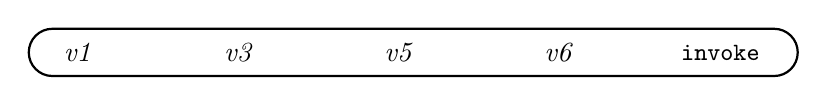
\begin{tikzpicture} [thick,
     rr/.style={rounded rectangle, fill=white, draw, minimum height=6mm, anchor=west}
   ]
% Use a matrix to establish positions, then paint stuff on top
\matrix [column sep=6mm, row sep=10mm]{
\node(v1){};&&&\node(v3){};&&&\node(v5){};&&&\node(v6){};&&\node(invoke){};\\
};
\node[rr, minimum width=10cm] at ($(v1.west) - (0.5cm,0)$) {};
\foreach \n in {v1,v3,v5,v6} {\node at (\n) {\it \n};};
\node[anchor=west] at (invoke) {\tt\small invoke};
\end{tikzpicture}
\end{center}
\caption{The temporary values used by \texttt{invoke}}
\end{figure}

In order for these uses to be in a loop, backtracking must be
initiated from outside; that is, beyond the subexpression (in the
example, only \texttt{\&fail} and \texttt{\&} are beyond the subexpression).

In addition, for an intermediate value to have an extended lifetime,
the beginning of the loop must start after the intermediate value is
computed. Two conditions may create the beginning of a loop. First,
the operation itself may be resumed. In this case, execution continues
forward within the operation. It may reuse any of its operands and
none of them are recomputed. The operation does not have to actually
generate more results. For example, reversible swap (the operator
{\textless}--{\textgreater}) can be resumed to reuse both of its
operands, but it does not generate another result. Whether an
operation actually reuses its operands on resumption depends on its
implementation. In the Icon compiler, operations implemented with a C
function using the standard calling conventions always use copies of
operands on resumption, but implementations tailored to a particular
use often reference operand locations on resumption.  Liveness
analysis is presented here as if all operations reuse their operands
on resumption. In the actual implementation, liveness analysis
computes a separate lifetime for values used internally by operations
and the code generator decides whether this lifetime applies to
operands. This internal lifetime may also be used when allocating
tended descriptors for variables declared local to the in-line code
for an operation. The behavior of the temporary-variable model
presented in this dissertation can be compared with one developed by
Nilsen and Martinek [.martinek.]; it also relies on the liveness
analysis described in this chapter.

The second way to create the beginning of a loop is for a
subexpression to generate results. Execution continues forward again
and any intermediate values to the left of the generative
subexpression may be reused without being recomputed.  Remember,
backtracking is initiated from outside the expression. Suppose an
expression that can fail is associated with \textit{v6}, in the
previous figure. This creates a loop with the generator associated
with \textit{v5}. However, this particular loop does not include
invoke and does not contribute to the reuse of \textit{v1} or
\textit{v3}.

A resumable operation and generative subexpressions are all
\textit{resumption points} within an expression. A simple rule can be
used to determine which intermediate values of an expression have
extended lifetimes: If the expression can be resumed, the intermediate
values with extended lifetimes consist of those to the left of the
rightmost resumption point of the expression. This rule refers to the
{\textasciigrave}{\textasciigrave}top level'{}' intermediate values.
The rule must be applied recursively to subexpressions to determine
the lifetime of lower level intermediate values.

It sometimes may be necessary to make conservative estimates of what
can fail and of resumption points (for liveness analysis, it is
conservative to overestimate what can fail or be resumed). For
example, invocation may or may not be resumable, depending on what is
being invoked and, in general, it cannot be known until run time what
is being invoked (for the purposes of this example analysis, it is
assumed that the variable write is not changed anywhere in the
program).

In the example, the rightmost operation that can fail is
\texttt{\&fail}. Resumption points are \texttt{!} and the
subexpressions corresponding to the intermediate values \textit{v5}
and \textit{v7}.

Once the resumption points have been identified, the rule for
determining extended lifetimes can be applied. If there are no
resumption points in an expression, no intermediate values in that
expression can be reused. Applying this rule to the postfix tree above
yields \textit{v1}, \textit{v3}, and \textit{v4} as the intermediate
values that have extended lifetimes.

Similar techniques can be used for liveness analysis of Prolog
programs, where goal-directed evaluation also creates implicit
loops. One difference is that a Prolog clause is a linear sequence of
calls. It does not need to be ``linearized'' by constructing a
postfix tree. Another difference is that all intermediate values in
Prolog programs are stored in explicit variables. A Prolog variable
has a lifetime that extends to the right of its last use if an
implicit loops starts after the variable's first use and ends after
the variable's last use.


\section[16.3 An Attribute Grammar]{16.3 An Attribute Grammar}

To cast this approach as an attribute grammar, an expression should be
thought of in terms of an abstract syntax tree.  The transformation
from a postfix tree to a syntax tree is trivial. It is accomplished by
deleting the explicit intermediate values. A syntax tree for the
example is:

%-% \includegraphics[width=3.1638in,height=3.198in]{kw/figure4-4.png}

\begin{figure}[htb]
\begin{center}
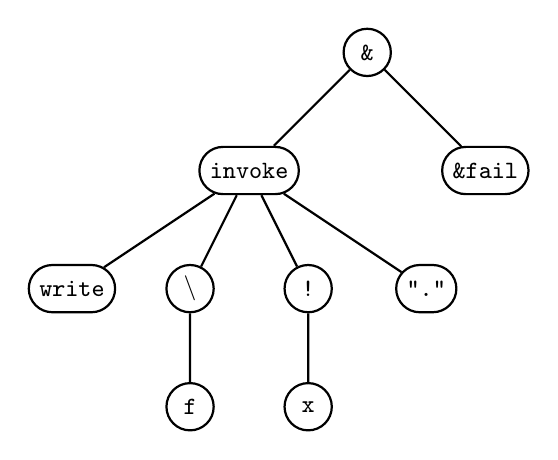
\begin{tikzpicture} [thick,font=\small\tt,
     rr/.style={rounded rectangle, fill=white, draw, minimum height=6mm}
   ]

\node (root) [rr] {\&}
  child
  { node[rr]{invoke}
    child { node [rr] {write} }
    child { node [rr] {\textbackslash}
            child { node[rr] {f}}
          }
    child { node [rr] {!} child { node[rr] {x} } }
    child {node [rr] {"."} }
  }
  child[missing]
  child { node[rr] {\&{}fail} };
\end{tikzpicture}
\end{center}
\caption{A syntax tree for \texttt{write({\textbackslash}f, !x, ".") \& \&fail}}
\end{figure}

Several interpretations can be given to a node in a syntax tree. A
node can be viewed as representing either an operation, an entire
subexpression, or an intermediate value.

This analysis associates four attributes with each node (this ignores
attributes needed to handle \texttt{break} expressions).  The goal of
the analysis is to produce the \texttt{lifetime} attribute. The other
three attributes are used to propagate information needed to compute
the \texttt{lifetime}.

\liststyleLxix
\begin{itemize}

\item \texttt{resumer} is either the rightmost operation (represented
as a node) that can initiate backtracking into the subexpression or it
is null if the subexpression cannot be resumed.

\item \texttt{failer} is related to \texttt{resumer}. It is the
rightmost operation that can initiate backtracking that can continue
past the subexpression. It is the same as \texttt{resumer}, unless the
subexpression itself contains the rightmost operation that can fail.

item \texttt{gen} is a boolean attribute. It is true if the
subexpression can generate multiple results if resumed.

\item \texttt{lifetime} is the operation beyond which the intermediate
value is no longer needed. It is either the parent node, the
\texttt{resumer} of the parent node, or null. The \texttt{lifetime} is
the parent node if the value is never reused after execution leaves
the parent operation. The \texttt{lifetime} is the \texttt{resumer} of
the parent if the parent operation or a generative sibling to the
right can be resumed. A lifetime of null is used to indicate that the
intermediate value is never used. For example, the value of the
control clause of an \texttt{if} expression is never used.

\end{itemize}

Attribute computations are associated with productions in the
grammar. The attribute computations for \texttt{failer} and
\texttt{gen} are always for the non-terminal on the left-hand side of
the production. These values are then used at the parent production;
they are effectively passed up the syntax tree. The computations for
\texttt{resumer} and \texttt{lifetime} are always for the attributes
of non-terminals on the right-hand side of the
production. \texttt{resumer} is then used at the productions defining
these non-terminals; it is effectively passed down the syntax
tree. \texttt{lifetime} is usually saved just for the code generator,
but it is sometimes used by child nodes.


\section[16.4 Primary Expressions]{16.4 Primary Expressions}

Variables, literals, and keywords are primary expressions. They have
no subexpressions, so their productions contain no computations for
\texttt{resumer} or \texttt{lifetime}. The attribute computations for
a literal follow. A literal itself cannot fail, so backtracking only
passes beyond it if the backtracking was initiated before (to the
right of) it. A literal cannot generate multiple results.

\goodbreak
\begin{iconcode}
\>expr ::= literal \>\>\>\>\ \{\\
\>\>\>\>\>\>expr.failer := expr.resumer\\
\>\>\>\>\>\>expr.gen := false\\
\>\>\>\>\>\ \}\\
\end{iconcode}



Another example of a primary expression is the keyword
\texttt{\&fail}. Execution cannot continue past \texttt{\&fail}, so it
must be the rightmost operation within its bounded expression that can
fail. A pre-existing attribute, \texttt{node}, is assumed to exist for
every symbol in the grammar. It is the node in the syntax tree that
corresponds to the symbol.

\goodbreak
\begin{iconcode}
\>expr ::= \&fail\>\>\>\> \{\\
\>\>\>\>\>\>expr.failer := expr.node\\
\>\>\>\>\>\>expr.gen := false\\
\>\>\>\>\>\}\\
\end{iconcode}


\section[16.5 Operations with Subexpressions]{16.5 Operations with Subexpressions}

Addition provides an example of the attribute computations involving
subexpressions. The following diagram shows how \texttt{resumer},
\texttt{failer}, and \texttt{gen} information would be passed through
the postfix tree.

%-% \noindent\includegraphics[width=5.9in,height=2.3in]{kw/figure4-5.png}

\begin{figure}[htb]
\begin{center}
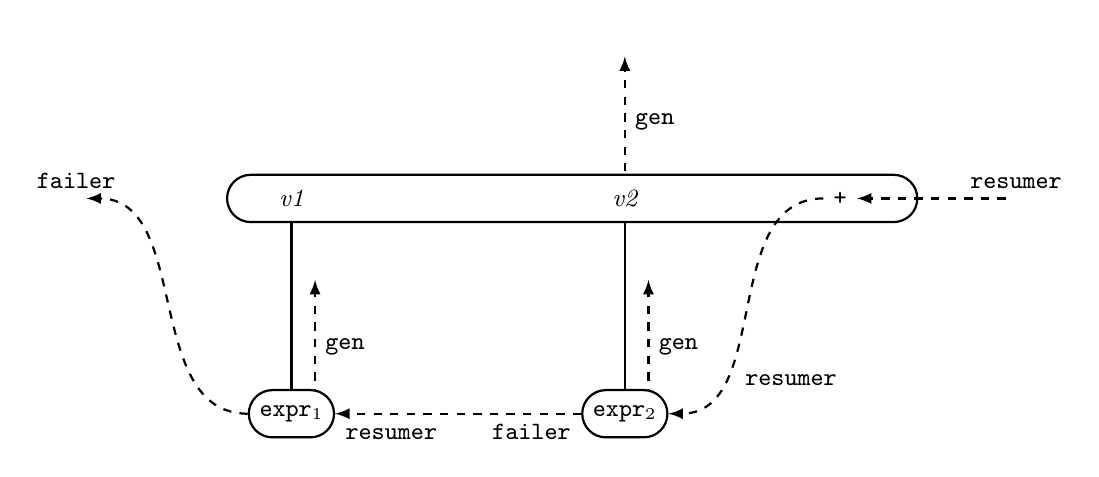
\begin{tikzpicture} [thick,>=latex, font=\small\tt,
     rr/.style={rounded rectangle, fill=white, draw, minimum height=6mm, anchor=west}
   ]
% Use a matrix to establish positions, then paint stuff on top
\matrix [column sep=20mm, row sep=20mm]{
&[5mm]&[20mm]\node(outT){};&[5mm]&\\[-3mm]
\node(outL){};&\node(v1){};&\node(v2){};&\node(pl){};&\node(inR){};\\[5mm]
&\node(ex1){};&\node(ex2){};&&\\
};
% Draw these lines before, so the rectangle shape masks them
\draw [dashed,->] (v2) to node[right] {gen} (outT);
\draw (ex1) -- (v1) (ex2) -- (v2);
\foreach \p in {ex1,ex2} {
  \draw [dashed,->] ($(\p) + (0.3cm,0)$) to node[right] {gen} ($(\p) + (0.3cm,1.7cm)$);
};
\node[rr, minimum width=9cm] at ($(v1.west) - (0.7cm,0)$) {};
\foreach \n in {v1,v2} {\node at (\n) {\it \n};};
\node (plus) at (pl) {+};
\node (expr1) [rr,anchor=center] at (ex1) {expr$_1$};
\node (expr2) [rr,anchor=center] at (ex2) {expr$_2$};
\draw [dashed,->] (plus.west) to[out=180,in=0] node[near end, right] {~resumer} (expr2.east);
\draw [dashed,->] (inR) -- (plus.east);
\node [above] at (inR) {resumer};
\draw [dashed,->] (expr2.west) to node[below]{resumer\hspace{0.7cm}failer} (expr1.east);
\draw [dashed,->] (expr1.west) to[out=180,in=0] (outL);
\node [above] at (outL) {failer};
\end{tikzpicture}
\end{center}
\caption{\label{p2-attInfo-PostfixTree}%
Passing attribute information through a postfix tree}
\end{figure}

This information would then be used to compute \texttt{lifetime}
information for \textit{v1} and \textit{v2}. Figure \ref{p2-attInfo-SyntaxTree} shows how
the attribute information is actually passed through the syntax tree.

%-% \includegraphics[width=6.0in,height=2.2in]{kw/figure4-6.png}  

%FLOAT! [DonW] LaTeX places this figure at the top of the next page
\begin{figure}[htb]
\begin{center}
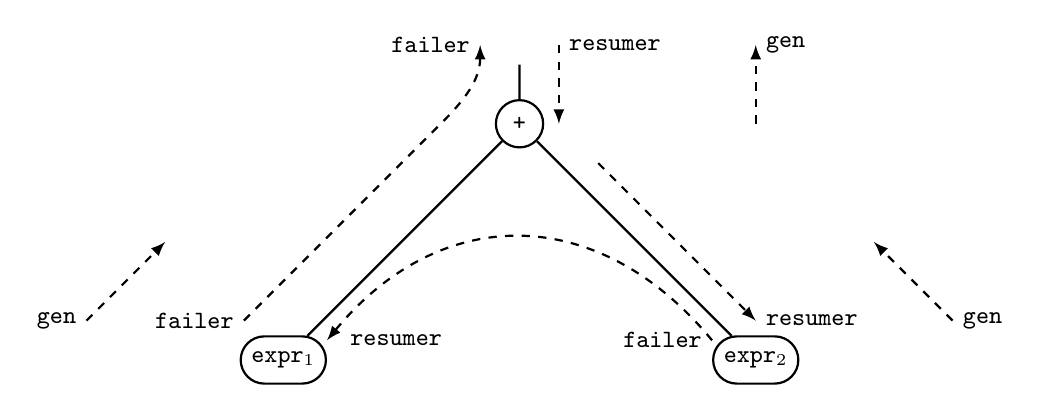
\begin{tikzpicture} [draw,thick,>=latex, font=\small\tt,
     rr/.style={rounded rectangle, fill=white, draw, minimum height=6mm}
   ]
% Draw the nodes
\node (pl) [rr] at (5,4) {+};
\node (e1) [rr] at (2,1) {expr$_1$};
\node (e2) [rr] at (8,1) {expr$_2$};
% connect the nodes
\draw (5,4.75) -- (pl) -- (e1) (pl) -- (e2);
% draw failer and resumer lines
\draw[dashed,->] (1.5,1.5) -- (4,4) to[in=270] (4.5,5) node[at start, left] {failer};
\draw[dashed,->] (5.5,5) -- ($(pl) + (0.5,0)$) node[at start, right] {resumer};
\node[xshift=0.5cm,anchor=east] at (4,5) {failer};
\draw[dashed,->] (6,3.5) -- ($(e2) + (0,0.5)$) node[at end,right] {resumer};
% Now the complicated bit: draw a nice bendy line between e2 and e1
\draw[dashed,->] ($(e2.west)+(0,0.25)$)
   .. controls (6,3) and (4,3)
   .. ($(e1.east)+(0,0.25)$)
   node[at start,left] {failer~} node[at end, right] {~resumer};
% Draw the "gen" lines
\draw[dashed,->] (8,4) -- (8,5) node[at end,right] {gen};
\draw[dashed,->] (10.5,1.5) -- (9.5,2.5) node[at start,right] {gen};
\draw[dashed,->] (-0.5,1.5) -- (0.5,2.5) node[at start,left] {gen};
\end{tikzpicture}
\end{center}
\caption{\label{p2-attInfo-SyntaxTree}%
Passing attribute information through a syntax tree}
\end{figure}

\noindent
The \texttt{lifetime} attributes are computed for the roots of the
subtrees for \texttt{expr}\TextSubscript{1} and
\texttt{expr}\TextSubscript{2}.


The details of the attribute computations depend, in part, on the
characteristics of the individual operation. Addition does not fail,
so the rightmost resumer, if there is one, of
\texttt{expr}\TextSubscript{2} is the rightmost resumer of the entire
expression. The rightmost resumer of \texttt{expr}\TextSubscript{1} is
the rightmost operation that can initiate backtracking that continues
past \texttt{expr}\TextSubscript{2}. Addition does not suspend, so the
lifetime of the value produced by \texttt{expr}\TextSubscript{2} only
extends through the operation (that is, it always is recomputed in the
presence of goal-directed evaluation). If
\texttt{expr}\TextSubscript{2} is a generator, then the result of
\texttt{expr}\TextSubscript{1} must be retained for as long as
\texttt{expr}\TextSubscript{2} might be resumed. Otherwise, it need
only be retained until the addition is
performed. \texttt{expr}\TextSubscript{1} is the first thing executed
in the expression, so its \texttt{failer} is the \texttt{failer} for
the entire expression. The expression is a generator if either
\texttt{expr}\TextSubscript{1} or \texttt{expr}\TextSubscript{2} is a
generator (note that the operation {\textbar} is logical \textit{or},
not Icon's alternation control structure):

\goodbreak
\begin{iconcode}
\>expr ::= expr\TextSubscript{1} + expr\TextSubscript{2} \{\\
\>\>\>\>\>expr\TextSubscript{2}.resumer := expr.resumer\\
\>\>\>\>\>expr\TextSubscript{2}.lifetime := expr.node\\
\>\>\>\>\>expr\TextSubscript{1}.resumer := expr\TextSubscript{2}.failer\\
\>\>\>\>\>if expr\TextSubscript{2}.gen \& (expr.resumer ${\neq}$ null) then\\
\>\>\>\>\>\>expr\TextSubscript{1}.lifetime := expr.resumer\\
\>\>\>\>\>else\\
\>\>\>\>\>\>expr\TextSubscript{1}.lifetime := expr.node\\
\>\>\>\>\>expr.failer := expr\TextSubscript{1}.failer\\
\>\>\>\>\>expr.gen := (expr\TextSubscript{1}.gen | expr\TextSubscript{2}.gen)\\
\>\>\>\>\>\}\\
\end{iconcode}


\texttt{/expr} provides an example of an operation that can fail. If
there is no rightmost resumer of the entire expression, it is the
rightmost resumer of the operand. The lifetime of the operand is
simply the operation, by the same argument used for
\texttt{expr}\TextSubscript{2} of addition. The computation of
\texttt{failer} is also analogous to that of addition. The expression
is a generator if the operand is a generator:

\goodbreak
\begin{iconcode}
\>expr ::= /expr\TextSubscript{1} \{\\
\>\>\>\>if expr.resumer = null then\\
\>\>\>\>\>expr\TextSubscript{1}.resumer := expr.node\\
\>\>\>\>else\\
\>\>\>\>\>expr\TextSubscript{1}.resumer := expr.resumer\\
\>\>\>\>expr\TextSubscript{1}.lifetime := expr.node\\
\>\>\>\>expr.failer := expr\TextSubscript{1}.failer\\
\>\>\>\>expr.gen := expr\TextSubscript{1}.gen\\
\>\>\>\>\}\\
\end{iconcode}


\texttt{!expr} differs from \texttt{/expr} in that it can generate
multiple results. If it can be resumed, the result of the operand must
be retained through the rightmost \texttt{resumer}:

\goodbreak
\begin{iconcode}
\>expr ::= !expr\TextSubscript{1} \{\\
\>\>\>\>if expr.resumer = null then \{\\
\>\>\>\>\>expr\TextSubscript{1}.resumer := expr.node\\
\>\>\>\>\>expr\TextSubscript{1}.lifetime := expr.node\\
\>\>\>\>\>\}\\
\>\>\>\>else \{\\
\>\>\>\>\>expr\TextSubscript{1}.resumer := expr.resumer\\
\>\>\>\>\>expr\TextSubscript{1}.lifetime := expr.resumer\\
\>\>\>\>\>\}\\
\>\>\>\>expr.failer := expr\TextSubscript{1}.failer\\
\>\>\>\>expr.gen := true\\
\>\>\>\>\}\\
\end{iconcode}


\section[16.6 Control Structures]{16.6 Control Structures}

Other operations follow the general pattern of the ones presented
above. Control structures, on the other hand, require unique attribute
computations. In particular, several control structures bound
subexpressions, limiting backtracking.  For example, \texttt{not}
bounds its argument and discards the value. If it has no
\texttt{resumer}, then it is the rightmost operation that can
fail. The expression is not a generator:

\goodbreak
\begin{iconcode}
\>expr ::= not expr\TextSubscript{1} \{\\
\>\>\>\>expr\TextSubscript{1}.resumer := null\\
\>\>\>\>expr\TextSubscript{1}.lifetime := null\\
\>\>\>\>if expr.resumer = null then\\
\>\>\>\>\>expr.failer := expr.node\\
\>\>\>\>else\\
\>\>\>\>\>expr.failer := expr.resumer\\
\>\>\>\>expr.gen := false\\
\>\>\>\>\}\\
\end{iconcode}


\texttt{expr}\TextSubscript{1} \texttt{; expr}\TextSubscript{2} bounds
\texttt{expr}\TextSubscript{1} and discards the result. Because the
result of \texttt{expr}\TextSubscript{2} is the result of the entire
expression, the code generator makes their result locations
synonymous. This is reflected in the lifetime computations. Indeed,
all the attributes of \texttt{expr}\TextSubscript{2} and those of the
expression as a whole are the same:

\goodbreak
\begin{iconcode}
\>expr ::= expr\TextSubscript{1} ; expr\TextSubscript{2} \{\\
\>\>\>\>\>expr\TextSubscript{1}.resumer := null\\
\>\>\>\>\>expr\TextSubscript{1}.lifetime := null\\
\>\>\>\>\>expr\TextSubscript{2}.resumer := expr.resumer\\
\>\>\>\>\>expr\TextSubscript{2}.lifetime := expr.lifetime\\
\>\>\>\>\>expr.failer := expr\TextSubscript{2}.failer\\
\>\>\>\>\>expr.gen := expr\TextSubscript{2}.gen\\
\>\>\>\>\>\}\\
\end{iconcode}


A reasonable implementation of alternation places the result of each
subexpression into the same location: the location associated with the
expression as a whole. This is reflected in the lifetime
computations. The resumer of the entire expression is also the resumer
of each subexpression. Backtracking out of the entire expression
occurs when backtracking out of \texttt{expr}\TextSubscript{2}
occurs. This expression is a generator:

\goodbreak
\begin{iconcode}
\>expr ::= expr\TextSubscript{1} | expr\TextSubscript{2} \{\\
\>\>\>\>\>expr\TextSubscript{2}.resumer:= expr.resumer\\
\>\>\>\>\>expr\TextSubscript{2}.lifetime := expr.lifetime\\
\>\>\>\>\>expr\TextSubscript{1}.resumer := expr.resumer\\
\>\>\>\>\>expr\TextSubscript{1}.lifetime := expr.lifetime\\
\>\>\>\>\>expr.failer := expr\TextSubscript{2}.failer\\
\>\>\>\>\>expr.gen := true\\
\>\>\>\>\>\}\\
\end{iconcode}


The first operand of an \texttt{if} expression is bounded and its
result is discarded. The other two operands are treated similar to
those of alternation. Because there are two independent execution
paths, the rightmost resumer may not be well-defined. However, it is
always conservative to treat the resumer as if it is farther right
than it really is; this just means that an intermediate value is kept
around longer than needed. If there is no resumer beyond the
\texttt{if} expression, but at least one of the branches can fail, the
failure is treated as if it came from the end of the \texttt{if}
expression (represented by the node for the expression). Because
backtracking out of an \texttt{if} expression is rare, this inaccuracy
is of little practical consequence. The \texttt{if} expression is a
generator if either branch is a generator:

\goodbreak
\begin{iconcode}
\>expr ::= if expr\TextSubscript{1} then expr\TextSubscript{2}~%
                                    else expr\TextSubscript{3} \{\\
\>\>\>\>\>expr\TextSubscript{3}.resumer := expr.resumer\\
\>\>\>\>\>expr\TextSubscript{3}.lifetime := expr.lifetime\\
\>\>\>\>\>expr\TextSubscript{2}.resumer := expr.resumer\\
\>\>\>\>\>expr\TextSubscript{2}.lifetime := expr.lifetime\\
\>\>\>\>\>expr\TextSubscript{1}.resumer := null\\
\>\>\>\>\>expr\TextSubscript{1}.lifetime := null\\
\>\>\>\>\>if expr.resumer = null \& (expr\TextSubscript{1}.failer $\neq$ null |~%
                                  expr\TextSubscript{2}.failer $\neq$ null) then\\
\>\>\>\>\>\>expr.failer := expr.node\\
\>\>\>\>\>else\\
\>\>\>\>\>\>expr.failer = expr.resumer\\
\>\>\>\>\>expr.gen := (expr\TextSubscript{2}.gen | expr\TextSubscript{3}.gen)\\
\>\>\>\>\>\}\\
\end{iconcode}


The \texttt{do} clause of \texttt{every} is bounded and its result
discarded. The control clause is always resumed at the end of the loop
and can never be resumed by anything else. The value of the control
clause is discarded. Ignoring \texttt{break} expressions, the loop
always fails:

\goodbreak
\begin{iconcode}
\>expr ::= every expr\TextSubscript{1} do expr\TextSubscript{2} \{\\
\>\>\>\>\>expr\TextSubscript{2}.resumer := null\\
\>\>\>\>\>expr\TextSubscript{2}.lifetime := null\\
\>\>\>\>\>expr\TextSubscript{1}.resumer := expr.node\\
\>\>\>\>\>expr\TextSubscript{1}.lifetime := null\\
\>\>\>\>\>expr.failer := expr.node\\
\>\>\>\>\>expr.gen := false\\
\>\>\>\>\>\}\\
\end{iconcode}


Handling \texttt{break} expressions requires some stack-like
attributes. These are similar to the ones used in the control flow
analyses described in O'Bagy's dissertation [.tr88-31.] and the ones
used to construct flow graphs in the original technical report on type
inferencing.

The attributes presented here can be computed with one walk of the
syntax tree. At a node, subtrees are processed in reverse execution
order: first the \texttt{resumer} and \texttt{lifetime} attributes of
a subtree are computed, then the subtree is walked. Next the
\texttt{failer} and \texttt{gen} attributes for the node itself are
computed, and the walk moves back up to the parent node.

\chapter{Overview of the Compiler}

\section{Components of the Compiler}

The Icon compiler is divided into two components: a run-time system
and the compiler itself. This organization is illustrated below. In
the diagram, labeled boxes represent programs, other text (some of it
delimited by braces) represents files, and arrows represent data flow.

%-%\noindent\includegraphics[width=6.0in,height=3.3in]{kw/figure5-1.png}

\begin{figure}[htb]
\noindent
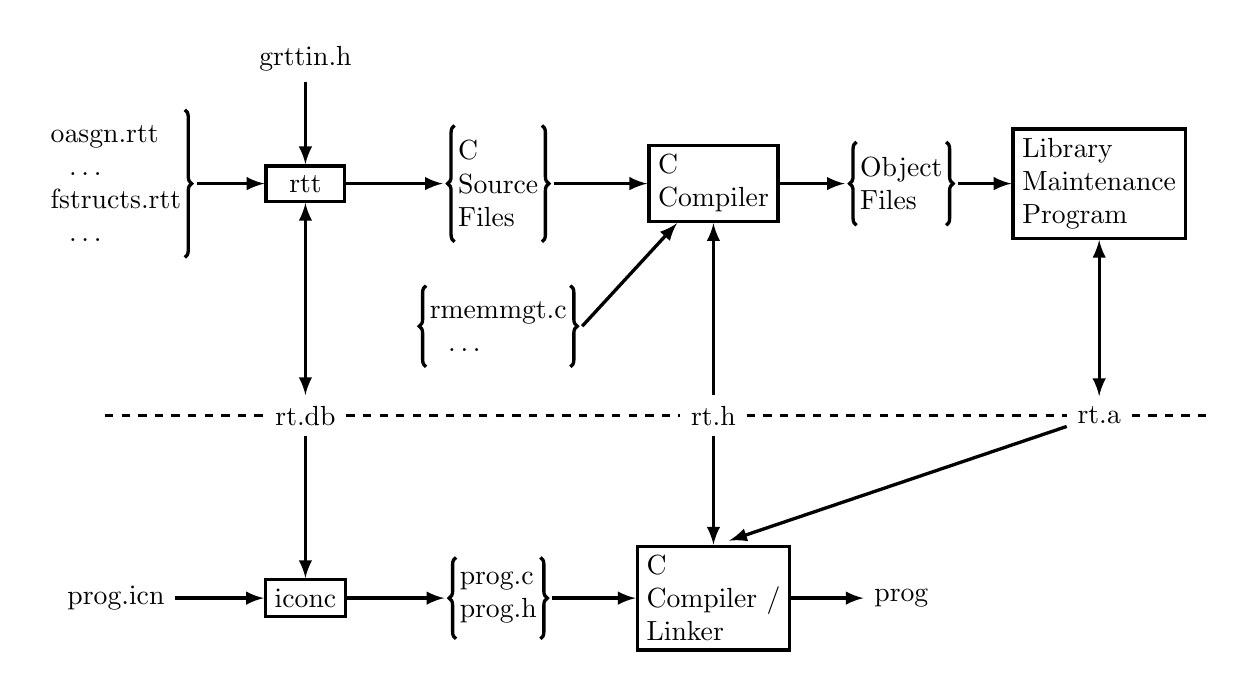
\begin{tikzpicture}[very thick, >=latex, arrows=->,
    box/.style={rectangle, minimum width=10mm, draw},
    txt/.style={align=left, inner sep=0.5em},
    tbox/.style={rectangle,draw,align=left},
  ]
\matrix[row sep=0.4cm, column sep=0.7cm]{
% Row 1
  & \node(gth) {grttin.h}; &  &  &  & &[-0.7cm]  \\
% Row 2
\node(rttf)[txt]{oasgn.rtt\\~~\ldots\\fstructs.rtt\\~~\ldots};
  & \node(rtt)[box] {rtt};
  & \node(csf)[txt] {C\\Source\\Files};
  & \node(cc) [tbox]{C\\Compiler};
  & \node(of) [txt] {Object\\Files};
  & \node(lmp)[tbox]{Library\\Maintenance\\Program};\\
% Row 3
  &  & \node(rmc)[txt] {rmemmgt.c\\~~\ldots};   &  &  &  \\
% Row 4
\node(ds){};  & \node(rtdb) {rt.db}; &  & \node(rth) {rt.h};  &  & \node(rta) {rt.a}; & \node(de){};\\[1cm]
% Row 5
\node(picn) {prog.icn};
  & \node(iconc)[box]{iconc};
  & \node(pch)[txt]{prog.c\\prog.h};
  & \node(ccl)[tbox]{C\\Compiler /\\Linker};
  & \node(prog){prog};& \\
};
\draw (gth) -- (rtt); \draw[<->] (rtt) -- (rtdb); \draw (rtdb) -- (iconc);
\draw[dashed,arrows=-] (ds.west) -- (rtdb) -- (rth) -- (rta) -- (de.east)[xshift=1cm];
\draw[<->] (lmp) -- (rta);
\draw (rth) -- (cc); \draw (rth) -- (ccl);
\draw (rmc.east) -- (cc);
\draw (rta) -- ($(ccl.north) + (0.2,0.05)$);


\draw[-,decorate,decoration=brace] ($(rttf.north east)-(0.15,0)$) -- ($(rttf.south east)-(0.15,0)$);
\foreach \n in {csf, rmc, pch, of} {
  \draw[-,decorate,decoration=brace] ($(\n.south west)+(0.15,0)$) -- ($(\n.north west)+(0.15,0)$);
  \draw[-,decorate,decoration=brace] ($(\n.north east)-(0.15,0)$) -- ($(\n.south east)-(0.15,0)$);
};
\draw (rttf.east) -- (rtt); \draw (rtt) -- (csf.west);
\draw (csf.east) -- (cc);   \draw (cc) -- (of.west); \draw (of.east) -- (lmp);

\draw (picn) -- (iconc);   \draw (iconc) -- (pch.west);
\draw (pch.east) -- (ccl); \draw (ccl) -- (prog);
\end{tikzpicture}
\caption{Organization of the compiler and run-time system}
\end{figure}

The run-time system appears above the dotted line and the compiler
itself appears below the line. The programs shown with the run-time
system are executed once when the run-time system is installed or
updated. They build a data base, rt.db, and an object-code library,
rt.a, for use by the compiler. The general definition of the term
{\textasciigrave}{\textasciigrave}data base'{}' is used here: a
collection of related data. rt.db is stored as a text file. It is
accessed and manipulated in internal tables by the programs rtt and
iconc. The rtt program is specific to the Icon compiler system and is
described below. The C compiler and the library maintenance program
are those native to the system on which the Icon compiler is being
used. The format of the object-code library is dictated by the linker
used with the C compiler. The file rt.h contains C definitions shared
by the routines in the run-time system and code generated by the
compiler.

The diagram of the compiler itself reflects the fact that the Icon
compiler uses a C compiler and linker as a back end.  However, iconc
automatically invokes these programs, so the Icon programmer sees a
single tool that takes Icon source as input and produces an executable
file.


\section{The Run-time System}

As with the run-time system for the interpreter, the run-time system
for the compiler implements Icon's operations.  However, the compiler
has needs beyond those of the interpreter. In the interpreter's
run-time system, all operations are implemented as C functions
conforming to certain conventions. The interpreter uses the same
implementation of an operation for all uses of the operation. While
this approach results in acceptable performance for many Icon
programs, the purpose of an optimizing compiler is to obtain better
performance. A major goal in the development of iconc is to use
information from type inferencing to tailor the parameter passing and
parameter type conversions of an operation to particular uses of the
operation and to place code in line where appropriate. The compiler
needs a mechanism to support this tailored operation invocation. In
addition, the compiler needs information about the properties of
operations for use in performing type inferencing and other analyses.

In addition to supporting the analyses and optimizations of iconc,
there are several other major goals in the design of the compiler's
run-time system. These include

\liststyleLxx
\begin{itemize}

\item Specification of all information about an operation in one place. 

\item Use of one coding to produce both general and tailored
implementation of an operation.

\item Use of the pre-existing run-time system as a basis for the new one. 

\end{itemize}

Most of the design goals for the run-time system would best be served
by a special-purpose language in which to implement the run-time
system. Such a language would allow the properties of an operation
needed by various analyses to be either explicitly coded or easily
inferred from parts of the code used to produce an implementation of
the operation. The language would also allow easy recognition and
manipulation of parts of the code that need to be tailored to
individual uses of an operation. In addition, the language would
provide support for features of Icon such as its data types and
goal-directed evaluation.

While a special-purpose language is consistent with most design goals,
it is not consistent with using the interpreter's run-time system
written in C as a basis for that of the compiler. A special-purpose
language also has the problem that it requires a large effort to
implement. These conflicting goals are resolved with a language that
is a compromise between an ideal special-purpose implementation
language and C. The core of the language is C, but the language
contains special features for specifying those aspects of a run-time
operation that must be dealt with by the compiler.  This language is
called the \textit{implementation language} for the Icon compiler's
run-time system. Because the implementation language is designed
around C, much of the detailed code for implementing an operation can
be borrowed from the interpreter system with only minor changes. The
important facets of the implementation language are discussed here. A
full description of the language can be found in the reference manual
for the language [.ipd79.]. The core material from this reference
manual is included as Appendix A of this dissertation.


\section{The Implementation Language}

The implementation language is used to describe the operators,
keywords, and built-in functions of Icon. In addition to these
operations, the run-time system contains routines to support other
features of Icon such as general invocation, co-expression activation,
and storage management. These other routines are written in C.

The program rtt takes as input files containing operations coded in
the implementation language and translates the operations into pure
C. rtt also builds the data base, rt.db, with information about the
operations. In addition to operations written in the implementation
language, rtt input may contain C functions. These C functions can use
several of the extensions available to the detailed C code in the
operations. These extensions are translated into ordinary C
code. While not critical to the goals of the run-time system design,
the ability to use these extensions in otherwise ordinary C functions
is very convenient.

The definition of an operation is composed of three layers. The outer
layer brackets the code for the operation. It consists of a header at
the beginning of the code and the reserved word end at the end of the
code. The header may be preceded by an optional description of the
operation in the form of a string literal; this description is used
only for documentation. The second layer consists of type checking and
type conversion code. Type checking code may be nested.  The inner
layer is the detailed C code, abstract type computations, and code to
handle run-time errors. An abstract type computation describes the
possible side-effects and result types of the operation in a form that
type inferencing can use. This feature is needed because it is
sometimes impractically difficult to deduce this information from the
C code. The code to handle run-time errors is exposed; that is, it is
not buried within the detailed C code. Because of this, type
inferencing can easily determine conditions under which an operation
terminates without either producing a value or failing. (A further
reason for exposing this code is explained in the implementation
language reference manual in the section on scoping.)

An operation header starts with one of the three reserved words
\texttt{operator}, \texttt{function}, or \texttt{keyword}.
The header contains a description of the operation's
\textit{result sequence}, that is, how many results it can produce.
This includes both the minimum and maximum number of results, with
\texttt{*} indicating an unbounded number. In addition, it indicates,
by a trailing \texttt{+}, when an operation can be resumed to perform
a side-effect after it has produced its last result. This information
is somewhat more detailed than can easily be inferred by looking at
the \texttt{returns}, \texttt{suspends}, and \texttt{fails} in the
detailed C code. The information is put in the data base for use by
the analysis phases of iconc.

An operation header also includes an identifier. This provides the
name for built-in functions and keywords. For all types of operations,
rtt uses the identifier to construct the names of the C functions that
implement the operations.  The headers for operators also include an
operator symbol. The parser for iconc is not required to use this
symbol for the syntax of the operation, but for most operations it
does so; list creation, \texttt{[\textit{\ldots}]}, is an example of an
exception. The headers for built-in functions and operators include a
parameter list. The list provides names for the parameters and
indicates whether dereferenced and/or undereferenced versions of the
corresponding argument are needed by the operation. It also indicates
whether the operation takes a variable number of arguments.


The following are five examples of operation headers. 

\goodbreak
\begin{iconcode}
\>function\{0,1+\} move(i)\\\\
\>function\{\} bal(c1,c2,c3,s,i,j)\\\\
\>operator\{1\} [...] llist(elems[n])\\\\
\>operator\{0,1\} / null(underef x --> dx)\\\\
\>keyword\{3\} regions
\end{iconcode}

\noindent
\texttt{move} is a function that takes one argument. It may produce
zero or one result and may be resumed to produce a side effect after
its last result. \texttt{bal} is a function that takes six arguments.
It produces an arbitrary number of results.  The list-creation operator
is given the symbol \texttt{[...]} (which may be used for string
invocation, if string invocation is enabled) and is given the name
\texttt{llist}. It takes an arbitrary number of arguments with
\texttt{elems} being the array of arguments and \texttt{n} being the
number of arguments. List creation always produces one result. The
\texttt{/} operator is given the name \texttt{null}.  It takes one
argument, but both undereferenced and dereferenced versions are needed
by the operation. It produces either zero or one result.
\texttt{\&regions} is a keyword that produces three results.

Type checking and type conversion constructs consist of an
\texttt{if-then} construct, an \texttt{if-then-else} construct, a
\texttt{type\_case} construct that selects code to execute based on
the type of an argument, and a \texttt{len\_case} construct that
selects code to execute based on the number of arguments in the
variable part of a variable-length argument list. The conditions in
the \texttt{if-then} and \texttt{if-then-else} constructs are composed
of operations that check the types of arguments or attempt to convert
arguments to specific types.

A type check starts with ``\texttt{is:}''. This is followed by the
name of a type and an argument in parentheses.  For example, the then
clause of the following \texttt{if} is executed if \texttt{x} is a
list.

\iconline{if is:list(x) then \textit{...} }

A type conversion is similar to a type check, but starts with
``\texttt{cnv:}''. For example, the following code attempts to convert
\texttt{s} to a string. If the conversion succeeds, the \texttt{then}
clause of the \texttt{if} is executed.

\iconline{if cnv:string(s) then \textit{...} }

There are forms of conversion that convert a null value into a
specified default value, forms that put a converted value in a
location other than the parameter, and forms that convert Icon values
into certain types of C values. The later type of conversion is
convenient because the detailed code is expressed in C. In addition,
exposing conversions back and forth between Icon and C values leaves
open the possibility of future optimizations to eliminate unnecessary
conversions to Icon values. The control clause of an \texttt{if} may
also use limited forms of expressions involving boolean operators. The
full syntax and semantics of conversions are described in the
implementation language reference manual.

Detailed code is expressed in a slightly extended version of C and is
introduced by one of two constructs. The first is

\iconline{inline \{ extended C \} }

This indicates that it is reasonable for the Icon compiler to put the
detailed code in line. The second construct is

\iconline{ \>body \{ extended C \} }

This indicates that the detailed code is too large to be put in line
and should only appear as part of a C function in the run-time
library. The person who codes the operation is free to decide which
pieces of detailed code are suitable to in-lining and which are
not. The decision is easily changed, so an operation can be fine tuned
after viewing the code produced by the compiler.

One extension to C is the ability to declare variables that are tended
with respect to garbage collection. Another extension is the ability
to use some constructs of the implementation language, such as type
conversions, within the C code. An important extension is the
inclusion of return, suspend, and fail statements that are analogous
to their Icon counterparts. This extension, combined with the
operation headers, makes the coding of run-time routines independent
of the C calling conventions used in the compiler system. The return
and suspend statements have forms that convert C values to Icon
values, providing inverses to conversions in the type checking code of
the implementation language.

This mechanism is more than is necessary for those keywords that are
simple constants. For keywords that are string, cset, integer, or real
constants there is a special form of definition. The Icon compiler
treats keywords coded with these definitions as manifest
constants. When future versions of the Icon compiler implement
constant folding, that optimization will be automatically applied to
these keywords.


\section{Standard and Tailored Operation Implementations}

For every operation that it translates, except keywords, rtt creates a
C function conforming to the standard calling conventions of the
compiler system. With the help of the C compiler and library
maintenance routine, rtt puts an object module for that function in
the compiler system's run-time library. This function is suitable for
invocation through a procedure block. It is used with unoptimized
invocations.

rtt creates an entry in the data base for every operation it
translates, including keywords. This entry contains the code for the
operation. The code is stored in the data base in a form that is
easier to parse and process than the original source, and the body
statements are replaced by calls to C functions. These C functions are
in the run-time library and implement the code from the body
statement. The calling conventions for these functions are tailored to
the needs of the code and do not, in general, conform to the standard
calling conventions of the compiler system.

When the compiler can determine that a particular operation is being
invoked, it locates the operation in the data base and applies
information from type inferencing to simplify or eliminate the code in
the operation that performs type checking and conversions on
arguments. These simplifications will eliminate detailed code that
will never be executed in this invocation of the operation. The
compiler can attempt the simplification because the type checking code
is in the data base in a form that is easily dealt with. If enough
simplification is possible, a tailored version of the operation is
generated in line. This tailored version includes the simplified type
checking code, if there is any left.  For detailed code that has not
been eliminated by the simplification, the tailored version also
includes the C code from inline statements and includes calls to the
functions that implement the code in body statements. The process of
producing tailored versions of built-in operations is described in
more detail in a later chapter.

Ideally, when unique types can be inferred for the operands of an
operation, the compiler should either produce a small piece of
type-specific in-line C code or produce a call to a type-specific C
function implementing the operation. It is possible to code operations
in the implementation language such that the compiler can do this. In
addition, this is the natural way to code most operations. For the few
exceptions, there are reasonable compromises between ideal generated
code and elegant coding in the implementation language. This
demonstrates that the design and implementation of the run-time system
and its communication with the compiler is successful.


\chapter{Organization of Iconc}

The Icon compiler, iconc, takes as input the source code for an Icon
program and, with the help of a C compiler and linker, produces an
executable file. The source code may be contained in several files,
but iconc does not support separate compilation. It processes an
entire program at once. This requirement simplifies several of the
analyses, while allowing them to compute more accurate
information. Without the entire program being available, the effects
of procedures in other files is unknown. In fact, it is not possible
to distinguish built-in functions from missing procedures. Type
inferencing would be particularly weakened. It would have to assume
that any call to an undeclared variable could have any side effect on
global variables (including procedure variables) and on any data
structure reachable through global variables or parameters.


\section[18.1 Compiler Phases]{18.1 Compiler Phases}

Iconc is organized into a number of phases. These are illustrated in
the diagram on the following page.

The initialization phase includes reading a data base of information
about run-time routines into internal tables. This information is used
in many of the other phases.

The source analysis phase consists of a lexical analyzer and
parser. These are adapted from those used in the interpreter
system. The parser generates abstract syntax trees and symbol tables
for all procedures before subsequent phases are invoked. The symbol
resolution phase determines the scope of variables that are not
declared in the procedures where they are used. This resolution can
only be done completely after all source files for the program are
read. If a variable does not have a local declaration, the compiler
checks to see whether the variable is declared global (possibly as a
procedure or record constructor) in one of the source files. If not,
the compiler checks to see whether the variable name matches that of a
built-in function. If the name is still not resolved, it is considered
to be a local variable.

\includegraphics[width=5.5484in,height=5.822in]{kw/figure6-1.png}  


\section[18.2 Naive Optimizations]{18.2 Naive Optimizations}

Naive optimizations involve invocation and assignment. These
optimizations are done before type inferencing to aid that
analysis. Certain ``debugging features'' of Icon such as the
variable function interfere with these optimizations. By default,
these features are disabled. If the user of iconc requests the
debugging features, these optimizations are bypassed. While these
optimizations are being done, information is gathered about whether
procedures suspend, return, or fail. This information is used in
several places in the compiler.

The invocation optimization replaces general invocation by a direct
form of invocation to a procedure, a built-in function, or a record
constructor. This optimization involves modifying nodes in the syntax
tree. It only applies to invocations where the expression being
invoked is a global variable initialized to a value in one of the
three classes of procedure values. First, the Icon program is analyzed
to determine which variables of this type appear only as the immediate
operands of invocations. No such variable is ever assigned to, so it
retains its initial value throughout the program (a more exact
analysis could be done to determine the variables that are not
assigned to, but this would seldom yield better results in real Icon
programs because these programs seldom do anything with procedure
values other that invoke them). This means that all invocations of
these variables can be replaced by direct invocations. In addition,
the variables themselves can be discarded as they are no longer
referenced.

The invocation optimization improves the speed of type inferencing in
two ways, although it does nothing to improve the accuracy of the
information produced. Performing type inferencing on direct
invocations is faster than performing it on general invocations. In
addition, type inferencing has fewer variables to handle, which also
speeds it up.

The invocation optimization does improve code generated by the
compiler. In theory, the optimization could be done better after type
inferencing using the information from that analysis, but in practice
this would seldom produce better results. On most real Icon programs,
this optimization using the naive analysis replaces all general
invocations with direct ones.

As noted in Chapter 3, it is important for type inferencing to
distinguish strong updates from weak updates. The data base contains a
general description of assignment, but it would be difficult for a
type inferencing system to use the description in recognizing that a
simple assignment or an augmented assignment to a named variable is a
strong update.  It is much easier to change general assignments where
the left hand side is a named variable to a special assignment and
have type inferencing know that the special assignment is a strong
update. Special-casing assignment to named variables is also important
for code generation. General optimizations to run-time routines are
not adequate to produce the desired code for these assignments. The
optimizations to assignment are described in Chapter 22.

The details of type inferencing are described in other
chapters. Producing code for the C main function, global variables,
constants, and record constructors is straightforward. C code is
written to two files for organizational purposes; it allows
definitions and code to be written in parallel.


\section[18.3 Code Generation for Procedures]{18.3 Code Generation for Procedures}

Producing code for procedures involves several sub-phases. The
sub-phases are liveness analysis, basic code generation, fix-up and
peephole optimization, and output. During this phase of code
generation, procedures are processed one at at time.

These sub-phases are described in later chapters. The code fix-up
phase and peephole optimization are performed during the same pass
over the internal representation of the C code. Some clean-up from
peephole optimization is performed when the code is written. The
logical organization of the compiler places the fix-up phase as a pass
in code generation with peephole optimization being a separate
phase. The organization of this dissertation reflects the logical
organization of the compiler rather than its physical organization.

The physical organization of this phase is shown in the following diagram.

\includegraphics[width=5.1311in,height=3.9063in]{kw/figure6-2.png} 


\bigskip


\bigskip


\chapter{The Implementation of Type Inferencing}

Chapter 15 develops a theoretical type inferencing model for Icon,
called Model 3. The purpose of that chapter is to explain the
relationship between type inferencing and the semantics of Icon; for
simplicity, some features of the language along with certain questions
of practical importance are ignored in that chapter. This chapter
describes the implementation of the type inferencing system used in
the Icon compiler. The implementation is based on Model 3. This
chapter describes solutions to those issues that must be addressed in
developing a complete practical type inferencing system from Model
3. The issues include:

\liststyleLxxi
\begin{itemize}
\item 
the representation of types and stores 
\item 
the development of a type system for the full Icon language 
\item 
the handing of procedure calls and co-expression activation 
\item 
the determination of edges in the flow graph 
\item 
the computation of a fixed point for type information 
\end{itemize}

In addition, performance of the abstract interpretation must be
considered. This includes both speed and memory usage.


\section[19.1 The Representation of Types and Stores]{19.1 The Representation of Types and Stores}

A type consists of a set of basic types (technically, it is a union of
basic types, but the constituents of the basic types are not
explicitly represented). The operations needed for these sets are: add
a basic type to a set, form the union of two sets, form the
intersection of two sets, test for membership in a set, and generate
members of a subrange of basic types (for example, generate all
members that are list types). A bit vector is used for the set
representation, with a basic type represented by an integer index into
the vector. The required operations are simple and efficient to
implement using this representation. Unless the sets are large and
sparse, this representation is also space efficient. While the sets of
types are often sparse, for typical programs, they are not large.

A store is implemented as an array of pointers to types. A mapping is
established from variable references to indexes in the store. In the
type inferencing model, Model 3, presented in Chapter 15, there is one
kind of store that contains all variables. In the actual
implementation, temporary variables need not be kept in this
store. The purpose of this store is to propagate a change to a
variable to the program points affected by the change. A temporary
variable is set in one place in the program and used in one place;
there is nothing to determine dynamically. It is both effective and
efficient to store the type of a temporary variable in the
corresponding node of the syntax tree.

Another level of abstraction can be developed that requires much less
memory than Model 3, but it must be modified to produce good
results. This abstraction abandons the practice of a store for every
edge in the flow graph. Instead it has a single store that is a merger
of all the stores in Model 3 (the type associated with a variable in a
merged store is the union of the types obtained for that variable from
each store being merged). For variables that are truly of one type
throughout execution, this abstraction works well. Named variables do
not have this property. They have an initial null value and usually
are assigned a value of another type during execution. Because
assignments to named variables are treated as strong updates, Model 3
can often deduce that a variable does not contain the null type at
specific points in the flow graph.

For structure variables this further abstraction does work well in
practice. These variables are initialized to the empty type (that is,
no instances of these variables exist at the start of program
execution), so the problem of the initial null type does not
occur. Sometimes instances of these variables are created with the
null type and later changed. However, the fact that assignments to
these variables must be treated as weak updates means that type
inferencing must assume that these variables can always retain their
earlier type after an assignment. Propagating type information about
structure variables through the syntax tree does not help much in
these circumstances. While it is possible to construct example
programs where Model 3 works better for structure variables than this
further abstraction, experiments with prototype type inferencing
systems indicate that the original system seldom gives better
information for real programs [.tr88-25.].

Type inferencing in the compiler is implemented with two kinds of
stores: local stores that are associated with edges in the flow graph
and contain named variables (both local and global variables) and a
global store that contains structure variables (in the implementation,
the global store is actually broken up by structure-variable type into
several arrays).


\section[19.2 A Full Type System]{19.2 A Full Type System}

Model 3 from Chapter 15 includes no structure type other than lists,
nor does it consider how to handle types for procedure and
co-expression values to allow effective type inferencing in their
presence. This section develops a complete and effective type system
for Icon.

Most of the structure types of Icon are assigned several subtypes in
the type inferencing system. As explained for lists in Chapter 15,
these subtypes are associated with the program points where values of
the type are created. The exception to this approach is records. One
type is created per record declaration. While it is possible to assign
a subtype to each use of a record constructor, in practice a given
kind of record usually is used consistently with respect to the types
of its fields throughout a program. The extra subtypes would require
more storage while seldom improving the resulting type information.

For efficiency, the size of the bit vectors representing types and the
size of the stores need to remain fixed during abstract
interpretation. This means that all subtypes must be determined as
part of the initialization of the type inferencing system. In order to
avoid excessive storage usage, it is important to avoid creating many
subtypes for program points where structures are not created. The
invocation optimization described in Chapter 19 helps determine where
structures can and cannot be created by determining for most
invocations what operation is used. The type inferencing system
determines what structures an operation can create by examining the
abstract type computations associated with the operation in the data
base. A new clause in an abstract type computation indicates that a
structure can be created. The following example is the abstract type
computation from the built-in function list. It indicates the the
function creates and returns a new list with elements whose type is
the same as that of the parameter \texttt{x} (the second parameter).

\goodbreak
\begin{iconcode}
\>abstract \{\\
\>\>return new list(type(x))\\
\>\>\}\\
\end{iconcode}

This is the clause as written by the programmer developing the
run-time library; it is translated into an internal form for storage
in the data base.

Invocation optimizations may not identify the operation associated
with some invocations. The initialization phase of type inferencing
skips these invocations. Type inferencing may later discover that one
of these invocations can create a structure. Each structure type is
given one subtype that is used for all of these later
discoveries. While it is possible for there to be several of these
creation points representing logically distinct subtypes, this seldom
occurs in practice. If it does happen, type inferencing produces a
correct, but less precise, result.

The type system contains representations for all run-time values that
must be modeled in the abstract interpretation.  These run-time values
can be divided into three categories, each of which is a superset of
the previous category:

\liststyleLxxii
\begin{itemize}
\item 
the first-class Icon values 
\item 
the intermediate values of expression evaluation 
\item 
the values used internally by Icon operations 
\end{itemize}

Just as these categories appear in different places during the
execution of an Icon program, the corresponding types appear in
different places during abstract interpretation. If certain types
cannot appear as the result of a particular type computation, it is
not necessary to have elements in the bit vector produced by the
computation to represent those types. It is particularly important to
minimize the memory used for stores associated with edges of the flow
graph (this is discussed more in the last section of this
chapter). These stores contain only the types of the smallest set
listed above: the first-class values.

Types (or subtypes) are allocated bit vector indexes. The first-class
types may appear as the result of any of the three classes of
computation. They are allocated indexes at the front of the bit
vectors. If they are the only types that can result from an abstract
computation, the bit vector for the result has no elements beyond that
of the last first-class types. The first-class types are:

\liststyleLxxiii
\begin{itemize}
\item 
null 
\item 
string 
\item 
cset 
\item 
integer 
\item 
real 
\item 
file 
\item 
list subtypes 
\item 
set subtypes 
\item 
table subtypes 
\item 
record subtypes 
\item 
procedure subtypes 
\item 
co-expression subtypes 
\end{itemize}

The list subtypes are allocated with 

\liststyleLxxiv
\begin{itemize}
\item 
one for the argument to the main procedure 
\item 
one for each easily recognized creation point 
\item 
one representing all other lists 
\end{itemize}

The set subtypes are allocated with 

\liststyleLxxv
\begin{itemize}
\item 
one for each easily recognized creation point 
\item 
one representing all other sets 
\end{itemize}

The table subtypes are allocated with 

\liststyleLxxvi
\begin{itemize}
\item 
one for each easily recognized creation point 
\item 
one representing all other tables 
\end{itemize}

The record subtypes are allocated with one for each record
declaration. The procedure subtypes are allocated with

\liststyleLxxvii
\begin{itemize}
\item 
one for each procedure 
\item 
one for each record constructor 
\item 
one for each built-in function 
\item 
one representing operators available for string invocation 
\end{itemize}

Note that procedure subtypes are allocated after most procedure and
function values have been eliminated by invocation optimizations (the
procedures and functions are still there, they are just not Icon
values). Therefore, few of these subtypes are actually allocated. The
co-expression subtypes are allocated with

\liststyleLxxviii
\begin{itemize}
\item 
one for the main co-expression 
\item 
one for each create expression 
\end{itemize}

The bit vectors used to hold the intermediate results of performing
abstract interpretation on expressions must be able to represent the
basic types plus the variable reference types. Variable reference
types are allocated bit vector indexes following those of the basic
types. The bit vectors for intermediate results are just long enough
to contain these two classifications of types. The variable reference
types are

\liststyleLxxix
\begin{itemize}
\item 
integer keyword variable types 
\item 
\texttt{\&pos} 
\item 
\texttt{\&subject}
\item 
substring trapped variable types 
\item 
table-element trapped variable types 
\item 
list-element reference types 
\item 
table assigned-value reference types 
\item 
field reference types 
\item 
global variable reference types 
\item 
local variable reference types 
\end{itemize}

\texttt{\&random} and \texttt{\&trace} behave the same way from the
perspective of the type inferencing system, so they are grouped under
one type as integer keyword variables. The fact that \texttt{\&pos}
can cause assignment to fail is reflected in the type inferencing
system, so it is given a separate type. \texttt{\&subject} is the only
string keyword variable so it is in a type by itself.

Substring trapped variables and table-element trapped variables are
``hidden'' structures in the implementation of Icon. They appear as
intermediate results, but are only indirectly observable in the
semantics of Icon. In order to reflect these semantics in the type
inferencing system, there are substring trapped variable types and
table-element trapped variable types. These are structure types
similar to sets, but are variable reference types rather than
first-class types. The substring trapped variable types are allocated
with

\liststyleLxxx
\begin{itemize}
\item 
one for each easily recognized creation point 
\item 
one representing all other substring trapped variables 
\end{itemize}

The table-element trapped variable types are allocated with 

\liststyleLxxxi
\begin{itemize}
\item 
one for each easily recognized creation point 
\item 
one representing all other table-element trapped variables 
\end{itemize}

List elements, table assigned-values, and record fields are all
variables that can appear as the intermediate results of expression
evaluation. The type system has corresponding variable reference types
to represent them. The list-element reference types are allocated with
one for each list types. The table assigned-value reference types are
allocated with one for each table type. The field reference types are
allocated with one for each record field declaration.

Identifiers are variables and are reflected in the type system. The
global variable reference types are allocated with

\liststyleLxxxii
\begin{itemize}
\item 
one for each global variable (except those eliminated by invocation optimizations). 
\item 
one for each static variable 
\end{itemize}

The local variable reference types are allocated with one for each
local variable, but the bit vector indexes and store indexes are
reused between procedures. The next section describes why this reuse
is possible.

Icon's operators use a number of internal values that never ``escape''
as intermediate results. Some of these internal values are reflected
in the type system in order to describe the semantics of the
operations in the abstract interpretation. The full set of types that
can be used to express these semantics are presented in the syntax of
the abstract type computations of the run-time implementation
language; see Appendix G. In addition to the types of intermediate
results, these types include

\liststyleLxxxiii
\begin{itemize}
\item 
set-element reference types 
\item 
table key reference types 
\item 
table default value reference types 
\item 
references to the fields within substring trapped variables that reference variables 
\item 
references to fields within table-element trapped variables that reference tables 
\end{itemize}

These types are allocated bit vector indexes at the end of the type
system. The only bit vectors large enough to contain them are the
temporary bit vectors used during interpretation of the abstract type
computations of built-in operations.

Set elements, table keys, and table default values do not appear as
variable references in the results of expression evaluation. However,
it is necessary to refer to them in order to describe the effects of
certain Icon operations. For this reason, they are included in the
type system. The set-element reference types are allocated with one
for each set type. The table key reference types are allocated with
one for each table type. The table default value reference types are
allocated with one for each table type.

Substring trapped variable types contain references to the variable
types being trapped and table-element trapped variable types contain
references to the table types containing the element being
trapped. These references are fields within these trapped variable
types. There is one field reference type for each trapped variable
type.


\section[19.3 Procedure Calls and Co-Expression Activations]{19.3 Procedure Calls and Co-Expression Activations}

A type inferencing system for the full Icon language must handle
procedures and co-expressions. As noted above, each procedure and each
create expression is given its own type. This allows the type
inferencing system to accurately determine which procedures are
invoked and what co-expressions might be activated by a particular
expression.

The standard semantics for procedures and co-expressions can be
implemented using stacks of procedure activation frames, with one
stack per co-expression. The first frame, on every stack except that
of the main co-expression, is a copy of the frame for the procedure
that created the co-expression. The local variables in this frame are
used for evaluating the code of the co-expression. The type
inferencing system uses a trivial abstraction of these procedure frame
stacks, while capturing the possible transfers of control induced by
procedure calls and co-expression activations.

The type inferencing system, in effect, uses an environment that has
one frame per procedure, where that frame is a summary of all frames
for the procedure that could occur in a corresponding environment of
an implementation of the standard semantics. The frame is simply a
portion of the store that contains local variables. Because no other
procedure can alter a local variable, it is unnecessary to pass the
types of local variables into procedure calls. If the called procedure
returns control via a return, suspend, or fail, the types are
unchanged, so they can be passed directly across the call. This allows
the type inferencing system to keep only the local variables of a
procedure in the stores on the edges of the flow graph for the
procedure, rather than keeping the local variables of all procedures.
Global variables must be passed into and out of procedure
calls. Because static variables may be altered in recursive calls,
they must also be passed into and out of procedure calls.

A flow graph for an entire program is constructed from the flow graphs
for its individual procedures and co-expressions.  An edge is added
from every invocation of a procedure to the head of that procedure and
edges are added from every return, suspend, and fail back to the
invocation. In addition, edges must be added from an invocation of a
procedure to all the suspends in the procedure to represent
resumption. When it is not possible to predetermine which procedure is
being invoked, edges are effectively added from the invocation to all
procedures whose invocation cannot be ruled out based on the naive
invocation optimizations. Edges are effectively added between all
co-expressions and all activations, and between all
activations. Information is propagated along an edge when type
inferencing deduces that the corresponding procedure call or
co-expression activation might actually occur. The representation of
edges in the flow graph is discussed below.

Type inferencing must reflect the initializations performed when a
procedure is invoked. Local variables are initialized to the null
value. On the first call to the procedure, static variables are also
initialized to the null value. The initialization code for the
standard semantics is similar to

\goodbreak
\begin{iconcode}
\>\textit{initialize locals}\\
\>if (first\_call) \{\\
\>\>initialize statics\\
\>\>user initialization code\\
\>\}\\
\end{iconcode}

In type inferencing, the variables are initialized to the null type
and the condition on the if is ignored. Type inferencing simply knows
that the first-call code is executed sometimes and not others. Before
entering the main procedure, global variables are set to the null type
and all static variables are set to the empty type. In some sense, the
empty type represents an impossible execution path. Type inferencing
sees paths in the flow graph from the start of the program to the body
of a procedure that never pass through the initialization
code. However, static variables have an empty type along this path and
no operation on them is valid. Invalid operations contribute nothing
to type information.


\section[19.4 The Flow Graph and Type Computations]{19.4 The Flow Graph and Type Computations}

In order to determine the types of variables at the points where they
are used, type inferencing must compute the contents of the stores
along edges in the flow graph. Permanently allocating the store on
each edge can use a large amount of memory. The usage is
\begin{displaymath}
  M = E (G + S + L) T / 8
\end{displaymath}
\begin{center}
\renewcommand{\arraystretch}{0.9}% Squeeze the lines together
\begin{tabular}{@{\hspace{1cm}}>{$\bgroup}l<{\egroup$}@{\hspace{3ex}---\hspace{3ex}}l}
M & total memory, expressed in bytes, used by stores.\\
E & the number of edges in the program flow graph.\\
G & the number of global variables in the program.\\
S & the number of static variables in the program.\\
L & the maximum number of local variables in any procedure.\\
T & the number of types in the type system.\\
\end{tabular}
\end{center}
  
\medskip\noindent
Large programs with many structure creation points can produce
thousands of edges, dozens of variables, and hundreds of types,
requiring megabytes of memory to represent the stores.

The code generation phase of the compiler just needs the (possibly
dereferenced) types of operands, not the stores. If dereferenced types
are kept at the expressions where they are needed, it is not necessary
to keep a store with each edge of the flow graph.

Consider a section of straight-line code with no
backtracking. Abstract interpretation can be performed on the graph
starting with the initial store at the initial node and proceeding in
execution order. At each node, the store on the edge entering the node
is used to dereference variables and to compute the next store if
there are side effects. Once the computations at a node are done, the
store on the edge entering the node is no longer needed. If updates
are done carefully, they can be done in-place, so that the same memory
can be used for both the store entering a node and the one leaving it.

In the case of branching control paths (as in a \texttt{case} expression),
abstract interpretation must proceed along one path at a time. The
store at the start the branching of paths must be saved for use with
each path. However, it need only be saved until the last path is
interpreted. At that point, the memory for the store can be
reused. When paths join, the stores along each path must be
merged. The merging can be done as each path is completed; the store
from the path can then be reused in interpreting other paths. When all
paths have been interpreted, the merged store becomes the current
store for the node at the join point.

The start of a loop is a point where control paths join. Unlike
abstract interpretation for the joining of simple branching paths,
abstract interpretation for the joining of back edges is not just a
matter of interpreting all paths leading to the join point before
proceeding. The edge leaving the start of the loop is itself on a path
leading to the start of the loop. Circular dependencies among stores
are handled by repeatedly performing the abstract interpretation until
a fixed point is reached. In this type inferencing system, abstract
interpretation is performed in iterations, with each node in the flow
graph visited once per iteration. The nodes are visited in execution
order. For back edges, the store from the previous iteration is used
in the interpretation. The stores on these edges must be kept
throughout the interpretation. These stores are initialized to map all
variables to the empty type. This represents the fact that the
abstract interpretation has not yet proven that execution can reach
the corresponding edge.

The type inferencing system never explicitly represents the edges of
the flow graph in a data structure. Icon is a structured programming
language. Many edges are implicit in a tree walk performed in forward
execution order -- the order in which type inferencing is
performed. The location of back edges must be predetermined in order
to allocate stores for them, but the edges themselves are effectively
recomputed as part of the abstract interpretation.

There are two kinds of back edges. The back edges caused by looping
control structures can be trivially deduced from the syntax tree. A
store for such an edge is kept in the node for the control
structure. Other back edges are induced by goal-directed
evaluation. These edges are determined with the same techniques used
in liveness analysis. A store for such an edge is kept in the node of
the suspending operation that forms the start of the loop. Because the
node can be the start of several nested loops, this store is actually
the merged store for the stores that theoretically exist on each back
edge.

At any point in abstract interpretation, three stores are of
interest. The \textit{current store} is the store entering the node on
which abstract interpretation is currently being performed. It is
created by merging the stores on the incoming edges. The
\textit{success store} is the store representing the state of
computations when the operation succeeds. It is usually created by
modifying the current store. The \textit{failure store} is the store
representing the state of computations when the operation fails.

In the presence of a suspended operation, the failure store is the
store kept at the node for that operation. A new failure store is
established whenever a resumable operation is encountered. This works
because abstract interpretation is performed in forward execution
order and resumption is LIFO. Control structures, such as
\texttt{if-then-else}, with branching and joining paths of execution, cause
difficulties because there may be more than one possible suspended
operation when execution leaves the control structure. This results in
more than one failure store during abstract interpretation. Rather
than keeping multiple failure stores when such a control structure has
operations that suspend on multiple paths, type inferencing pretends
that the control structure ends with an operation that does nothing
other than suspend and then fail. It allocates a store for this
operation in the node for the control structure. When later operations
that fail are encountered, this store is updated. The failure of this
imaginary operation is the only failure seen by paths created by the
control structure and the information needed to update the failure
stores for these paths is that in the store for this imaginary
operation. This works because the imaginary operation just passes
along failure without modifying the store.


In the case where a control structure transforms failure into forward
execution, as in the first subexpression of a compound expression, the
failure store is allocated (with empty types) when the control
structure is encountered and deallocated when it is no longer
needed. If no failure can occur, no failure store need be
allocated. The lack of possible failure is noted while the location of
back edges is being computed during the initialization of type
inferencing. Because a failure store may be updated at several
operations that can fail, these are weak updates.  Typically, a
failure store is updated by merging the current store into it.

The interprocedural flow graph described earlier in this chapter has
edges between invocations and returns, suspends, and fails. Type
inferencing does not maintain separate stores for these theoretical
edges. Instead it maintains three stores per procedure that are
mergers of stores on several edges. One store is the merger of all
stores entering the procedure because of invocation; this store
contains parameter types in addition to the types of global and static
variables. Another store is the merger of all stores entering the
procedure because of resumption. The third store is the merger of all
stores leaving the procedure because of returns, suspends, and
fails. There is also a result type associated with the procedure. It
is updated when abstract interpretation encounters returns and
suspends.

Two stores are associated with each co-expression. One is the merger
of all stores entering the co-expression and the other is the merger
of all stores leaving the co-expression. Execution can not only leave
through an activation operator, it can also re-enter through the
activation. The store entering the activation is a merger of the
stores entering all co-expressions in which the activation can
occur. Because a procedure containing an activation may be called from
several co-expressions, it is necessary to keep track of those
co-expressions. A set of co-expressions is associated with each
procedure for this purpose. Each co-expression also contains a type
for the values transmitted to it. The result type of an activation
includes the result types for all co-expressions that might be
activated and the types of all values that can be transmitted to a
co-expression that the activation might be executed in.

When type inferencing encounters the invocation of a built-in
operation, it performs abstract interpretation on the representation
of the operation in the data base. It interprets the type-checking
code to see what paths might be taken through the operation. The
interpretation uses the abstract type computations and ignores the
detailed C code when determining the side effects and result type of
the operation. Because the code at this level of detail contains no
loops, it is not necessary to save stores internal to operations. An
operation is re-interpreted at each invocation.  This allows type
inferencing to produce good results for polymorphous operations. At
this level, the code for an operation is simple enough that the cost
of re-interpretation is not prohibitive. All side effects within these
operations are treated as weak updates; the only strong updates
recognized by type inferencing are the optimized assignments to named
variables (see Chapter 18).

The abstract semantics of control structures are hard-coded within the
type inferencing system. The system combines all the elements
described in this chapter to perform the abstract interpretation. A
global flag is set any time an update changes type information that is
used in the next iteration of abstract interpretation. The flag is
cleared between iterations. If the flag is not set during an
iteration, a fixed point has been reached and the interpretation
halts.

\chapter{Code Generation}

This chapter describes the code generation process. The examples of
generated code presented here are produced by the compiler, but some
cosmetic changes have been made to enhance readability.

Code generation is done one procedure at a time. An Icon procedure is,
in general, translated into several C functions. There is always an
\textit{outer function}
for the procedure. This is the function that is seen as implementing
the procedure. In addition to the outer function, there may be several
functions for success continuations that are used to implement
generative expressions.

The outer function of a procedure must have features that support the
semantics of an Icon call, just as a function implementing a run-time
operation does. In general, a procedure must have a procedure block at
run time. This procedure block references the outer function. All
functions referenced through a procedure block must conform to the
compiler system's standard calling conventions. However, invocation
optimizations usually eliminate the need for procedure variables and
their associated procedure blocks. When this happens, the calling
conventions for the outer function can be tailored to the needs of the
procedure.

As explained in Chapter 14, the standard calling convention requires
four parameters: the number of arguments, a pointer to the beginning
of an array of descriptors holding the arguments, a pointer to a
result location, and a success continuation to use for suspension. The
function itself is responsible for dereferencing and argument list
adjustment.  In a tailored calling convention for an outer function of
a procedure, any dereferencing and argument list adjustment is done at
the call site. This includes creating an Icon list for the end of a
variable-sized argument list. The compiler produces code to do this
that is optimized to the particular call. An example of an
optimization is eliminating dereferencing when type inferencing
determines that an argument cannot be a variable reference.

The number of arguments is never needed in these tailored calling
conventions because the number is fixed for the procedure. Arguments
are still passed via a pointer to an array of descriptors, but if
there are no arguments, no pointer is needed. If the procedure returns
no value, no result location is needed. If the procedure does not
suspend, no success continuation is needed.

In addition to providing a calling interface for the rest of the
program, the outer function must provide local variables for use by
the code generated for the procedure. These variables, along with
several other items, are located in a procedure frame. An Icon
procedure frame is implemented as a C structure embedded within the
frame of its outer C function (that is, as a local struct
definition). Code within the outer function can access the procedure
frame directly. However, continuations must use a pointer to the
frame. A global C variable, \texttt{pfp}, points to the frame of the currently
executing procedure. For efficiency, continuations load this pointer
into a local register variable. The frame for a main procedure might
have the following declaration.

\goodbreak
\begin{iconcode}
struct PF00\_main \{\\
\>struct p\_frame old\_pfp;\\
\>dptr old\_argp;\\
\>dptr rslt;\\
\>continuation succ\_cont;\\
\>struct \{\\
\>\>struct tend\_desc *previous;\\
\>\>int num;\\
\>\>struct descrip d[5];\\
\>\>\} tend;\\
\>\};\\
\end{iconcode}

\noindent with the definition

\iconline{ \>struct PF00\_main frame; }

\noindent in the procedure's outer function. A procedure frame always
contains the following five items: a pointer to the frame of the
caller, a pointer to the argument list of the caller, a pointer to the
result location of this call, a pointer to the success continuation of
this call, and an array of tended descriptors for this procedure. It
may also contain C integer variables, C double variables, and string
and cset buffers for use in converting values. If debugging is
enabled, additional information is stored in the frame. The structure
\texttt{p\_frame} is a generic procedure frame containing a single
tended descriptor. It is used to define the pointer \texttt{old\_pfp}
because the caller can be any procedure.

The argument pointer, result location, and success continuation of the
call must be available to the success continuations of the
procedure. A global C variable, \texttt{argp}, points the argument list for the
current call. This current argument list pointer could have been put
in the procedure frame, but it is desirable to have quick access to
it. Quick access to the result location and the success continuation
of the call is less important, so they are accessed indirectly through
the procedure frame.

The array of descriptors is linked onto the chain used by the garbage
collector to locate tended descriptors. These descriptors are used for
Icon variables local to the procedure and for temporary variables that
hold intermediate results. If the function is responsible for
dereferencing and argument list adjustment (that is, if it does not
have a tailored calling convention), the modified argument list is
constructed in a section of these descriptors.

The final thing provided by the outer function is a \textit{control
environment} in which code generation starts. In particular, it
provides the bounding environment for the body of the procedure and
the implicit failure at the end of the procedure. The following C
function is the tailored outer function for a procedure named
\texttt{p}. The procedure has arguments and returns a result. However,
it does not suspend, so it needs no success continuation.

\goodbreak
\begin{iconcode}
static int P01\_p(args, rslt)\\
dptr args;\\
dptr rslt;\\
\{\\
\>struct PF01\_p frame;\\
\>register int signal;\\
\>int i;\\
\>frame.old\_pfp = pfp;\\
\>pfp = (struct p\_frame )\&frame;\\
\>frame.old\_argp = argp;\\
\>frame.rslt = rslt;\\
\>frame.succ\_cont = NULL;\\
\\
\>for (i = 0; i < 3; ++i)\\
\>\>frame.tend.d[i].dword = D\_Null;\\
\>argp = args;\\
\>frame.tend.num = 3;\\
\>frame.tend.previous = tend;\\
\>tend = (struct tend\_desc )\&frame.tend;\\
\\
\>\textit{translation of the body of procedure p}\\
\\
L10: /* bound */\\
L4: /* proc fail */\\
\>tend = frame.tend.previous;\\
\>pfp = frame.old\_pfp;\\
\>argp = frame.old\_argp;\\
\>return A\_Resume;\\
L8: /* proc return */\\
\>tend = frame.tend.previous;\\
\>pfp = frame.old\_pfp;\\
\>argp = frame.old\_argp;\\
\>return A\_Continue;\\
\>\}\\
\end{iconcode}

\noindent
The initialization code reflects the fact that this function has three
tended descriptors to use for local variables and intermediate
results. \texttt{L10} is both the bounding label and the failure label for the
body of the procedure. Code to handle procedure failure and return
(except for setting the result value) is at the end of the outer
function. As with bounding labels, the labels for these pieces of code
have associated signals. If a procedure fail or return occurs in a
success continuation, the continuation returns the corresponding
signal which is propagated to the outer function where it is converted
into a goto. The code for procedure failure is located after the body
of the procedure, automatically implementing the implicit failure at
the end of the procedure.


\section[20.1 Translating Icon Expressions]{20.1 Translating Icon Expressions}

Icon's goal-directed evaluation makes the implementation of control
flow an important issue during code generation. Code for an expression
is generated while walking the expression's syntax tree in forward
execution order. During code generation there is always a
\textit{current failure action}. This action is either ``branch to a
label'' or ``return a signal''.  When the translation of a procedure
starts, the failure action is to branch to the bounding label of the
procedure body. The action is changed when generators are encountered
or while control structures that use failure are being translated.

The allocation of temporary variables to intermediate results is
discussed in more detail later. However, some aspects of it will be
addressed before presenting examples of generated code. The result
location of a subexpression may be determined when the parent
operation is encountered on the way down the syntax tree. This is
usually a temporary variable, but does not have to be. If no location
has been assigned by the time the code generator needs to use it, a
temporary variable is allocated for it. This temporary variable is
used in the code for the parent operation.

The code generation process is illustrated below with examples that
use a number of control structures and operations.  Code generation
for other features of the language is similar.

Consider the process of translating the following Icon expression: 

\iconline{return if a = (1 | 2) then "yes" else "no" }

\noindent
When this expression is encountered, there is some current failure
action, perhaps a branch to a bounding label. The \texttt{return}
expression produces no value, so whether a result location has been
assigned to it is of no consequence. If the argument of a
\texttt{return} fails, the procedure fails. To handle this
possibility, the current failure action is set to branch to the label
for procedure failure before translating the argument (in this
example, that action is not used).  The code for the argument is then
generated with its result location set to the result location of the
procedure itself. Finally the result location is dereferenced and
control is transferred to the procedure return label. The
dereferencing function, \texttt{deref}, takes two arguments: a pointer
to a source descriptor and a pointer to a destination descriptor.

\goodbreak
\begin{iconcode}
\>\>\textit{code for the if expression }\\
\>\>deref(rslt, rslt);\\
\>\>goto L7 /* proc return */;\\
\end{iconcode}


The control clause of the \texttt{if} expression must be bounded. The
code implementing the \texttt{then} clause must be generated following
the bounding label for the control clause. A label must also be set up
for the \texttt{else} clause with a branch to this label used as the
failure action for the control clause. Note that the result location
of each branch is the result location of the \texttt{if} expression
which is in turn the result location of the procedure. Because neither
branch of the \texttt{if} expression contains operations that suspend,
the two control paths can be brought together with a branch to a
label.

\goodbreak
\begin{iconcode}
\>\>\textit{code for control clause}\\
\>L4: /* bound */\\
\>\>rslt->vword.sptr = "yes";\\
\>\>rslt->dword = 3;\\
\>\>goto L6 /* end if */;\\
\>L5: /* else */\\
\>\>rslt->vword.sptr = "no";\\
\>\>rslt->dword = 2;\\
\>L6: /* end if */\\
\end{iconcode}

\noindent
Using a branch and a label to bring together the two control paths of
the \texttt{if} expression is an optimization. If the \texttt{then} or
the \texttt{else} clauses contain operations that suspend, the general
continuation model must be used. In this model, the code following the
\texttt{if} expression is put in a success continuation, which is then
called at the end of both the code for the \texttt{then} clause and
the code for the \texttt{else} clause.

Next consider the translation of the control clause. The numeric
comparison operator takes two operands. In this translation, the
standard calling conventions are used for the library routine
implementing the operator. Therefore, the operands must be in an array
of descriptors. This array is allocated as a sub-array of the tended
descriptors for the procedure. In this example, tended location 0 is
occupied by the local variable, \texttt{a}. Tended locations 1 and 2 are free
to be allocated as the arguments to the comparison operator. The code
for the first operand simply builds a variable reference.

\goodbreak
\begin{iconcode}
\>frame.tend.d[1].dword = D\_Var;\\
\>frame.tend.d[1].vword.descptr = \&frame.tend.d[0] /* a */;\\
\end{iconcode}

\noindent
However, the second operand is alternation. This is a generator and
requires a success continuation. In this example, the continuation is
given the name \texttt{P02\_main} (the Icon expression is part of the main
procedure). The continuation contains the invocation of the run-time
function implementing the comparison operator and the end of the
bounded expression for the control clause of the \texttt{if}. The function
\texttt{O0o\_numeq} implements the comparison operator. The \texttt{if} expression
discards the operator's result. This is accomplished by using the
variable \texttt{trashcan} as the result location for the call. The compiler
knows that this operation does not suspend, so it passes a null
continuation to the function. The end of the bounded expression
consists of a transfer of control to the bounding label. This is
accomplished by returning a signal. The continuation is

\goodbreak
\begin{iconcode}
static int P02\_main()\\
\{\\
register struct PF00\_main *rpfp;\\

rpfp = (struct PF00\_main *)pfp;\\
switch (O0o\_numeq(2, \&(rpfp->tend.d[1]), \&trashcan, (continuation)NULL))\\
\>\{\\
\>case A\_Continue:\\
\>\>break;\\
\>case A\_Resume:\\
\>\>return A\_Resume;\\
\>\}\\
\ return 4; /* bound */\\
\}\\
\end{iconcode}

\noindent
Each alternative of the alternation must compute the value of its
subexpression and call the success continuation. The failure action
for the first alternative is to branch to the second alternative. The
failure action of the second alternative is the failure action of the
entire alternation expression. In this example, the failure action is
to branch to the \texttt{else} label of the \texttt{if} expression. In
each alterative, a bounding signal from the continuation must be
converted into a branch to the bounding label. Note that this bounding
signal indicates that the control expression succeeded.

\goodbreak
\begin{iconcode}
frame.tend.d[2].dword = D\_Integer;\\
frame.tend.d[2].vword.integr = 1;\\
switch (P02\_main()) \{\\
\>case A\_Resume:\\
\>\>goto L2 /* alt */;\\
\>case 4 /* bound */:\\
\>\>goto L4 /* bound */;\\
\>\}\\
L2: /* alt */\\
\>frame.tend.d[2].dword = D\_Integer;\\
\>frame.tend.d[2].vword.integr = 2;\\
\>switch (P02\_main()) \{\\
\>\>case A\_Resume:\\
\>\>\>goto L5 /* else */;\\
\>\>case 4 /* bound */:\\
\>\>\>goto L4 /* bound */;\\
\>\>\}\\
\end{iconcode}


The code for the entire \texttt{return} expression is obtained by putting
together all the pieces. The result is the following code (the code
for \texttt{P02\_main} is not repeated).

\goodbreak
\begin{iconcode}
frame.tend.d[1].dword = D\_Var;\\
frame.tend.d[1].vword.descptr = \&frame.tend.d[0] /* a */;\\
frame.tend.d[2].dword = D\_Integer;\\
frame.tend.d[2].vword.integr = 1;\\
switch (P02\_main()) \{\\
\>case A\_Resume:\\
\>\>goto L2 /* alt */;\\
\>case 4 /* bound */:\\
\>\>goto L4 /* bound */;\\
\>\}\\
L2: /* alt */\\
\>frame.tend.d[2].dword = D\_Integer;\\
\>frame.tend.d[2].vword.integr = 2;\\
\>switch (P02\_main()) \{\\
\>\>case A\_Resume:\\
\>\>\>goto L5 /* else */;\\
\>\>case 4 /* bound */:\\
\>\>\>goto L4 /* bound */;\\
\>\>\}\\
L4: /* bound */\\
\>rslt->vword.sptr = yes;\\
\>rslt->dword = 3;\\
\>goto L6 /* end if */;\\

L5: /* else */\\
\>rslt->vword.sptr = no;\\
\>rslt->dword = 2;\\
L6: /* end if */\\
\>deref(rslt, rslt);\\
\>goto L7 /* proc return */;\\
\end{iconcode}


\section[20.2 Signal Handling]{20.2 Signal Handling}

In order to produce signal handling code, the code generator must know
what signals may be returned from a call. These signals may be either
directly produced by the operation (or procedure) being called or they
may originate from a success continuation. Note that either the
operation or the continuation may be missing from a call, but not
both. The signals produced directly by an operation are
\texttt{A\_Resume}, \texttt{A\_Continue}, and \texttt{A\_FallThru}
(this last signal is only used internally within in-line code).

The signals produced by a success continuation belong to one of three
categories: \texttt{A\_Resume}, signals corresponding to labels within the
procedure the continuation belongs to, and signals corresponding to
labels in procedures farther down in the call chain. The last category
only occurs when the procedure suspends. The success continuation for
the procedure call may return a signal belonging to the calling
procedure. This is demonstrated in the following example (the
generated code has been ``cleaned-up'' a little to make it easier to
follow).  The Icon program being translated is

\goodbreak
\begin{iconcode}
procedure main()\\
\>write(p())\\
end\\
procedure p()\\
\>suspend 1 to 10\\
end\\
\end{iconcode}


The generative procedure \texttt{p} is called in a bounded context. The code
generated for the call is

\goodbreak
\begin{iconcode}
switch (P01\_p(\&frame.tend.d[0], P05\_main)) \{\\
\>case 7 /* bound */:\\
\>\>goto L7 /* bound */;\\
\>case A\_Resume:\\
\>\>goto L7 /* bound */;\\
\>\}\\
L7: /* bound */\\
\end{iconcode}

\noindent
This call uses the following success continuation. The continuation
writes the result of the call to \texttt{p} then signals the end of the bounded
expression.

\goodbreak
\begin{iconcode}
static int P05\_main() \{\\
\>register struct PF00\_main *rpfp;\\
\\
\>rpfp = (struct PF00\_main )pfp;\\
\>F0c\_write(1, \&rpfp->tend.d[0], \&trashcan, (continuation)NULL);\\
\>return 7; /* bound */\\
\}\\
\end{iconcode}

\noindent
The \texttt{to} operator in procedure \texttt{p} needs a success
continuation that implements procedure suspension. Suspension is
implemented by switching to the old procedure frame pointer and old
argument pointer, then calling the success continuation for the call
to \texttt{p}. The success continuation is accessed with the
expression \texttt{rpfp--{\textgreater}succ\_cont}.  In this example,
the continuation will only be the \texttt{function P05\_main}. The
suspend must check the signal returned by the procedure call's success
continuation. However, the code generator does not try to determine
exactly what signals might be returned by a continuation belonging to
another procedure. Such a continuation may return an
\texttt{A\_Resume} signal or a signal belonging to some procedure
farther down in the call chain. In this example, bounding signal 7
will be returned and it belongs to \texttt{main}.

If the call's success continuation returns \texttt{A\_Resume}, the procedure
frame pointer and argument pointer must be restored, and the current
failure action must be executed. In this case, that action is to
return an \texttt{A\_Resume} signal to the \texttt{to} operator. If the call's success
continuation returns any other signal, that signal must be propagated
back through the procedure call. The following function is the success
continuation for the \texttt{to} operator.

\goodbreak
\begin{iconcode}
static int P03\_p()\\
\{\\
\>register int signal;\\
\>register struct PF01\_p *rpfp;\\
\\
\>rpfp = (struct PF01\_p *)pfp;\\
\>deref(rpfp->rslt, rpfp->rslt);\\
\>pfp = rpfp->old\_pfp;\\
\>argp = rpfp->old\_argp;\\
\\
\>signal = (*rpfp->succ\_cont)();\\
\>if (signal != A\_Resume) \{\\
\>\>return signal;\\
\>\>\}\\
\>pfp = (struct p\_frame *)rpfp;\\
\>argp = NULL;\\
\>return A\_Resume;\\
\}\\
\end{iconcode}


The following code implements the call to the \texttt{to}
operator. The signal handling code associated with the call must pass
along any signal from the procedure call's success continuation. These
signals are recognized by the fact that the procedure frame for the
calling procedure is still in effect. At this point, the signal is
propagated out of the procedure \texttt{p}. Because the procedure
frame is about to be removed from the C stack, the descriptors it
contains must be removed from the tended list.

\goodbreak
\begin{iconcode}
frame.tend.d[0].dword = D\_Integer;\\
frame.tend.d[0].vword.integr = 1;\\
frame.tend.d[1].dword = D\_Integer;\\
frame.tend.d[1].vword.integr = 10;\\
signal = O0k\_to(2, \&frame.tend.d[0], rslt, P03\_p);\\
if (pfp != (struct p\_frame )\&frame) \{\\
\>tend = frame.tend.previous;\\
\>return signal;\\
\>\}\\
switch (signal) \{\\
\>case A\_Resume:\\
\>\>goto L2 /* bound */;\\
\>\}\\
L2: /* bound */\\
\end{iconcode}


So far, this discussion has not addressed the question of how the code
generator determines what signals might be returned from a
call. Because code is generated in execution order, a call involving a
success continuation is generated before the code in the continuation
is generated. This makes it difficult to know what signals might
originate from the success continuation. This problem exists for
direct calls to a success continuation and for calls to an operation
that uses a success continuation.

The problem is solved by doing code generation in two parts. The first
part produces incomplete signal handling code. At this time, code to
handle the signals produced directly by an operation is generated. The
second part of code generation is a fix-up pass that completes the
signal handling code by determining what signals might be produced by
success continuations.

The code generator constructs a call graph of the continuations for a
procedure. Some of these calls are indirect calls to a continuation
through an operation. However, the only effect of an operation on
signals returned by a continuation is to intercept \texttt{A\_Resume}
signals. All other signals are just passed along. This is true even if
the operation is a procedure. This call graph of continuations does
not contain the procedure call graph nor does it contain continuations
from other procedures.

Forward execution order imposes a partial order on continuations. A
continuation only calls continuations strictly greater in forward
execution order than itself. Therefore the continuation call graph is
a DAG.

The fix-up pass is done with a bottom-up walk of the continuation call
DAG. This pass determines what signals are returned by each
continuation in the DAG. While processing a continuation, the fix-up
pass examines each continuation call in that continuation. At the
point it processes a call, it has determined what signals might be
returned by the called continuation. It uses this information to
complete the signal handling code associated with the call and to
determine what signals might be passed along to continuations higher
up the DAG. If a continuation contains code for a \texttt{suspend}, the fix-up
pass notes that the continuation may return a \textit{foreign} signal
belonging to another procedure call. As explained above, foreign
signals are handled by special code that checks the procedure frame
pointer.


\section[20.3 Temporary Variable Allocation]{20.3 Temporary Variable Allocation}

The code generator uses the liveness information for an intermediate
value when allocating a temporary variable to hold the value. As
explained in Chapter 16, this information consists of the furthest
program point, represented as a node in the syntax tree, through which
the intermediate value must be retained. When a temporary variable is
allocated to a value, that variable is placed on a
\textit{deallocation list} associated with the node beyond which its
value is not needed. When the code generator passes a node, all the
temporary variables on the node's deallocation list are deallocated.

The code generator maintains a \textit{status array} for temporary
variables while it is processing a procedure. The array contains one
element per temporary variable. This array is expandable, allowing a
procedure to use an arbitrary number of temporary variables. In a
simple allocation scheme, the status of a temporary variable is either
\textit{free} or \textit{in-use}. The entry for a temporary variable
is initially marked free, it is marked in-use when the variable is
allocated, and it is marked free again when the variable is
deallocated.

The simple scheme works well when temporary variables are allocated
independently. It does not work well when arrays of contiguous
temporary variables are allocated. This occurs when temporary
variables are allocated to the arguments of a procedure invocation or
any invocation conforming to the standard calling conventions; under
these circumstances, the argument list is implemented as an array. All
of the contiguous temporary variables must be reserved before the
first one is used, even though many operations may be performed before
the last one is needed. Rather than mark a temporary variable in-use
before it actually is, the compiler uses the program point where the
temporary variable will be used to mark the temporary variable's entry
in the status array as \textit{reserved}. A contiguous array of
temporary variables are marked reserved at the same time, with each
having a different reservation point. A reserved temporary variable
may be allocated to other intermediate values as long as it will be
deallocated before the reservation point. In this scheme, an entry in
a deallocation list must include the previous status of the temporary
variable as it might be a reserved status.

The compiler allocates a contiguous subarray of temporary variables
for the arguments of an invocation when it encounters the invocation
on the way down the syntax tree during its tree walk. It uses a
first-fit algorithm to find a large enough subarray that does not have
a conflicting allocation. Consider the problem of allocating temporary
variables to the expression

\iconline{ \>f1(f2(f3(x, f4())), y) }

\noindent where \texttt{f1} can fail and \texttt{f4} is a
generator. The syntax tree for this expression is shown below. Note
that invocation nodes show the operation as part of the node label and
not as the first operand to general invocation. This reflects the
direct invocation optimization that is usually performed on
invocations. Each node in the graph is given a numeric label. These
labels increase in value in forward execution order.

{\centering\selectlanguage{english}
\includegraphics[width=3.0in,height=3.0in]{kw/figure8-1.png}
\par}

The following figure shows the operations in forward execution order
with lines on the left side of the diagram showing the lifetime of
intermediate values. This represents the output of the liveness
analysis phase of the compiler. Because \texttt{f4} can be resumed by
\texttt{f1}, the value of the expression \texttt{x} has a lifetime
that extends to the invocation of \texttt{f1}. The extended portion of
the lifetime is indicated with a dotted line.

{\centering\selectlanguage{english}
\includegraphics[width=1.3in,height=1.6in]{kw/figure8-2.png}
\par}


The following series of diagrams illustrate the process of allocating
intermediate values. Each diagram includes an annotated syntax tree
and a status array for temporary variables. An arrow in the tree shows
the current location of the tree walk. A deallocation list is located
near the upper right of each node. An element in the list consists of
a temporary variable number and the status with which to restore the
variable's entry in the status array. If a temporary variable has been
allocated to an intermediate value, the variable's number appears near
the lower right of the corresponding node.

The status array is shown with four elements. The elements are
initialized to \textit{F} which indicates that the temporary variables
are free. A reserved temporary variable is indicated by placing the
node number of the reservation point in the corresponding
element. When a temporary variable is actually in use, the
corresponding element is set to \textit{I}.

Temporary variables are reserved while walking down the syntax
tree. The tree illustrated below on the left shows the state of
allocation after temporary variables have been allocated for the
operands of \texttt{f1}. Two contiguous variables are needed. All
variables are free, so the first-fit algorithm allocates variables 0
and 1. The status array is updated to indicate that these variables
are reserved for nodes \textit{4} and \textit{5} respectively, and the
nodes are annotated with these variable numbers. The lifetime
information in the previous figure indicates that these variables
should be deallocated after \texttt{f1} is executed, so the
deallocation array for node \textit{6} is updated.

The next step is the allocation of a temporary variable to the operand
of \texttt{f2}. The intermediate value has a lifetime extending from node
\textit{3} to node \textit{4}. This conflicts with the allocation of
variable 0, but not the allocation of variable 1. Therefore, variable
1 is allocated to node \textit{3} and the deallocation list for node
\textit{4} is updated. This is illustrated in the tree on the right:

{\centering\selectlanguage{english}
\includegraphics[width=6.0in,height=4.2in]{kw/figure8-3.png}
\par}

The final allocation requires a contiguous pair of variables for nodes
\textit{1} and \textit{2}. The value from node \textit{1} has a
lifetime that extends to node \textit{6}, and the value from node
\textit{2} has a lifetime that extends to node \textit{3}. The current
allocations for variables 0 and 1 conflict with the lifetime of the
intermediate value of node \textit{1}, so the variables 2 and 3 are
used in this allocation. This is illustrated in the tree:

{\centering\selectlanguage{english}
\includegraphics[width=3.6in,height=5.0in]{kw/figure8-5.png}
\par}


The remaining actions of the allocator in this example mark temporary
variables in-use when the code generator uses them and restore
previous allocated statuses when temporary variables are
deallocated. This is done in the six steps illustrated in the
following diagram. The annotations on the graph do not change. Only
the node of interest is shown for each step. These steps are performed
in node-number order.

{\centering\selectlanguage{english}
 \includegraphics[width=6.0in,height=3.3in]{kw/figure8-6.png}  
\par}


In general, the tree walk will alternate up and down the syntax
tree. For example, if node \textit{5} had children, the allocation
status after the deallocation associated with node \textit{4},

{\centering\selectlanguage{english}
 \includegraphics[width=1.2in,height=0.6in]{kw/figure8-6-5.png}  
\par}

\noindent is used to allocate temporary variables to those
children. If this requires more than four temporary variables, the
status array is extended with elements initialized to \textit{F}.

This allocation algorithm is not guaranteed to produce an allocation
that uses a minimal number of temporary variables.  Indeed, a smaller
allocation for the previous example is illustrated in the tree:

{\centering\selectlanguage{english}
\includegraphics[width=3.3in,height=3.7in]{kw/figure8-7.png}  
\par}


While the non-optimality of this algorithm is unlikely to have a
measurable effect on the performance of any practical program, the
problem of finding an efficient optimal solution is of theoretical
interest. Classical results in the area of register allocation do not
apply. It is possible to allocate a minimum number of registers from
expression trees for conventional languages in polynomial time
[.dragon.]. The algorithm to do this depends on the fact that
registers (temporary variables) are dead as soon as the value they
contain is used. This is not true for Icon temporary variables.

The result of Prabhala and Sethi stating that register allocation is
NP-complete even in the presence of an infinite supply of registers
also does not apply [.prabhala subexp.]. Their complexity result
derives from performing register allocation in the presence of common
subexpression elimination (that is, from performing register
allocation on expression DAGS rather than trees) on a
2-address-instruction machine with optimality measured as the minimum
number of instructions needed to implement the program. Goal-directed
evaluation imposes more structure on lifetimes than common
subexpression elimination, the machine model used here is the C
language, and optimality is being measure as the minimum number of
temporary variables needed.

The Icon temporary variable allocation problem is different from the
Prolog variable allocation problem. Prolog uses explicit variables
whose lifetimes can have arbitrary overlaps even in the absence of
goal-directed evaluation. The Prolog allocation problem is equivalent
to the classical graph coloring problem which is NP-complete [.debray
apr91, dragon.].

If the allocation of a subarray of temporary variables is delayed
until the first one is actually needed in the generated code, an
optimum allocation results for the preceding example. It is not
obvious whether this is true for the general case of expression trees
employing goal-directed evaluation. This problem is left for future
work.

In addition to holding intermediate values, temporary variables are
used as local tended variables within in-line code.  This affects the
pattern of allocations, but not the underlying allocation technique.

\chapter{Control Flow Optimizations}

\section{Naive Code Generation}

Naive code generation does not consider the effects and needs of the
immediately surrounding program. The result is often a poor use of the
target language. Even sophisticated code generation schemes that
consider the effects of relatively large pieces of the program still
produce poor code at the boundaries between the pieces. This problem
is typically solved by adding a \textit{peephole optimizer} to the
compiler to improve the generated code [.peep1,Wulf,Tanenbaum
peephole,dragon.]. A peephole optimizer looks at several instructions
that are adjacent (in terms of execution) and tries to replace the
instructions by better, usually fewer, instructions. It typically
analyzes a variety of properties of the instructions such as
addressing modes and control flow.

The Icon compiler has a peephole optimizer that works on the internal
form of the generated C code and deals only with control flow. The
previous examples of generated code contain a number of instances of
code where control flow can be handled much better. For example, it is
possible to entirely eliminate the following code fragment generated
for the example explaining procedure suspension.

\goodbreak
\begin{iconcode}
\>switch (signal) \{\\
\>\>case A\_Resume:\\
\>\>\>goto L2 /* bound */;\\
\>\}\\
L2: /* bound */\\
\end{iconcode}

\noindent
This code is produced because the code generator does not take into
account the fact that the bounding label happens to immediately follow
the test.


\section{Success Continuations}

For the C code in the preceding example, it is quite possible that a C
compiler would produce machine code that its own peephole optimizer
could eliminate. However, it is unlikely that a C compiler would
optimize naively generated success continuations. An earlier example
of code generation produced the continuation:

\goodbreak
\begin{iconcode}
static int P02\_main()\\
\{\\
\>register struct PF00\_main *rpfp;\\
\\
\>rpfp = (struct PF00\_main *)pfp;\\
\>switch (O0o\_numeq(2, \&(rpfp->tend.d[1]), \&trashcan, (continuation)NULL)) \{\\
\>\>case A\_Continue:\\
\>\>\>break;\\
\>\>case A\_Resume:\\
\>\>\>return A\_Resume;\\
\>\>\}\\
\>return 4; /* bound */\\
\}\\
\end{iconcode}

\noindent
If the statement 

\iconline{return 4; /* bound */ }

\noindent
is brought into the \texttt{switch} statement, replacing the
\texttt{break}, then \texttt{P02\_main} consists of a simple operation
call (a C call with associated associated signal handling code). This
operation call is

\goodbreak
\begin{iconcode}
switch (O0o\_numeq(2, \&(rpfp->tend.d[1]), \&trashcan, (continuation)NULL)) \{\\
\>case A\_Continue:\\
\>\>return 4; /* bound */\\
\>case A\_Resume:\\
\>\>return A\_Resume;\\
\}\\
\end{iconcode}

\noindent
\texttt{P02\_main} is called directly in two places in the following code. 

\goodbreak
\begin{iconcode}
frame.tend.d[2].dword = D\_Integer;\\
frame.tend.d[2].vword.integr = 1;\\
switch (P02\_main()) \{\\
\>case A\_Resume:\\
\>\>goto L2 /* alt */;\\
\>case 4 /* bound */:\\
\>\>goto L4 /* bound */;\\
\>\}\\
L2: /* alt */\\
\>frame.tend.d[2].dword = D\_Integer;\\
\>frame.tend.d[2].vword.integr = 2;\\
\>switch (P02\_main()) \{\\
\>\>case A\_Resume:\\
\>\>\>goto L5 /* else */;\\
\>\>case 4 /* bound */:\\
\>\>\>goto L4 /* bound */;\\
\>\>\}\\
L4: /* bound */\\
\end{iconcode}


A direct call to a trivial function can reasonably be replaced by the
body of that function. When this is done for a continuation, it is
necessary to \textit{compose} the signal handling code of the body of
a continuation with that of the call. This is accomplished by
replacing each return statement in the body with the action in the
call corresponding to the signal returned. The following table
illustrates the signal handling composition for the first call in the
code.  The resulting code checks the signal from \texttt{O0o\_numeq} and
performs the final action.

\begin{center}
\tablefirsthead{}
\tablehead{}
\tabletail{}
\tablelasttail{}
%\begin{xtabular}{|m{1.8in}|m{1.8in}|m{1.1in}|}
\begin{xtabular}{|c|c|c|}
\hline
~~signal from \texttt{O0o\_numeq}~~  &
~~signal from \texttt{P02\_main}~~  &
~~final action~~ \\\hline
\texttt{A\_Continue} & 4                  & \texttt{goto L4;}\\
\texttt{A\_Resume}   & \texttt{A\_Resume} & \texttt{goto L2;}\\\hline
\end{xtabular}
\end{center}

\noindent
The result of in-lining \texttt{P02\_main} is 

\goodbreak
\begin{iconcode}
frame.tend.d[2].dword = D\_Integer;\\
frame.tend.d[2].vword.integr = 1;\\
switch (O0o\_numeq(2, \&frame.tend.d[1], \&trashcan, (continuation)NULL)) \{\\
\>case A\_Continue:\\
\>\>goto L4 /* bound */;\\
\>case A\_Resume:\\
\>\>goto L2 /* alt */;\\
\>\}\\
L2: /* alt */\\
\>frame.tend.d[2].dword = D\_Integer;\\
\>frame.tend.d[2].vword.integr = 2;\\
\>switch (O0o\_numeq(2, \&frame.tend.d[1], \&trashcan,%
                    (continuation)NULL)) \{\\
\>\>case A\_Continue:\\
\>\>\>goto L4 /* bound */;\\
\>\>case A\_Resume:\\
\>\>\>goto L5 /* else */;\\
\>\}\\
L4: /* bound */\\
\end{iconcode}

With a little more manipulation, the \texttt{switch} statements can be
converted into \texttt{if} statements and the label \texttt{L2} can be
eliminated:

\goodbreak
\begin{iconcode}
frame.tend.d[2].dword = D\_Integer;\\
frame.tend.d[2].vword.integr = 1;\\
if (O0o\_numeq(2, \&frame.tend.d[1], \&trashcan,%
              (continuation)NULL) == A\_Continue)\\
\>goto L4 /* bound */;\\
frame.tend.d[2].dword = D\_Integer;\\
frame.tend.d[2].vword.integr = 2;\\
if (O0o\_numeq(2, \&frame.tend.d[1], \&trashcan,%
              (continuation)NULL) == A\_Resume)\\
\>goto L5 /* else */;\\
L4: /* bound */\\
\end{iconcode}


The Icon compiler's peephole optimizer recognizes two kinds of trivial
continuations. The kind illustrated in the previous example consists
of a single call with associated signal handling. The other kind
simply consists of a single return-signal statement. As in the above
example, continuations do not usually meet this definition of
triviality until control flow optimizations are performed on them. For
this reason, the Icon compiler's peephole optimizer must perform some
optimizations that could otherwise be left to the C compiler.


\section{Iconc's Peephole Optimizer}

The peephole optimizer performs the following optimizations: 

\liststyleLxxxiv
\begin{itemize}
\item 
elimination of unreachable code 
\item 
elimination of gotos immediately preceding their destinations 
\item 
collapse of branch chains 
\item 
deletion of unused labels 
\item 
collapse of trivial call chains (that is, in-lining trivial continuations) 
\item 
deletion of unused continuations 
\item 
simplification of signal checking 
\end{itemize}

Unreachable code follows a \texttt{goto} or a \texttt{return}, and it
continues to the first referenced label or to the end of the function.
This optimization may eliminate code that returns signals, thereby
reducing the number of signals that must be handled by a continuation
call. This provides another reason for performing this traditional
optimization in the Icon compiler rather than letting the C compiler
do it. This code is eliminated when the fix-up pass for signal
handling is being performed. \texttt{goto}s immediately preceding their labels
also are eliminated at this time.

Unused labels usually are eliminated when the code is written out, but
they may be deleted as part of a segment of unreachable code. Unused
continuations are simply not written out.

A branch chain is formed when the destination of a \texttt{goto} is
another \texttt{goto} or a \texttt{return}. A \texttt{break} in a
\texttt{switch} statement is treated as a \texttt{goto}. There may be
several \texttt{goto}s in a chain. Each \texttt{goto} is replaced by
the \texttt{goto} or \texttt{return} at the end of the chain. This may
leave some labels unreferenced and may leave some of the intermediate
\texttt{goto}s unreachable. Branch chains are collapsed during the
fix-up pass.

Inter-function optimization is not traditionally considered a peephole
optimization. This is because human beings seldom write trivial
functions and most code generators do not produce continuations. The
Icon compiler, however, uses calls to success continuations as freely
as it uses \texttt{goto}s. Therefore collapsing trivial call chains is
as important as collapsing branch chains.

There are two kinds of calls to trivial continuations: direct calls
and indirect calls through an operation. A direct call always can be
replaced by the body of the continuation using signal handling code
that is a composition of that in the continuation and that of the
call. If the continuation consists of just a \texttt{return}
statement, this means that the call is replaced by the action
associated with the returned signal: either another \texttt{return}
statement or a \texttt{goto} statement. For continuations consisting
of a call, the composition is more complicated, as demonstrated by the
example given earlier in this chapter.

In the case of an indirect call through an operation, the continuation
cannot be placed in line. However, there is an optimization that can
be applied. Under some circumstances, the compiler produces a
continuation that simply calls another continuation. For example, this
occurs when compiling the Icon expression

\iconline{every write(!x | end) }

The compiler allocates a continuation for the alternation, then
compiles the expression \texttt{!x}. The element generation operator
suspends, so the compiler allocates a continuation for it and code
generation proceeds in this continuation.  However, the end of the
first alternative has been reached so the only code for this
continuation is a call to the continuation for the alternation. The
continuation for the alternation contains the code for the invocation
of \texttt{write} and for the end of the \texttt{every} control
structure. The code for the first alternative is

\goodbreak
\begin{iconcode}
frame.tend.d[2].dword = D\_Var;\\
frame.tend.d[2].vword.descptr = \&frame.tend.d[0] /* x */;\\
\\
switch (O0e\_bang(1, \&frame.tend.d[2], \&frame.tend.d[1], P02\_main)) \{\\
\>case A\_Resume:\\
\>\>goto L1 /* alt */;\\
\>\}\\
\ L1: /* alt */\\
\end{iconcode}

\noindent
The code for the two continuations are 

\goodbreak
\begin{iconcode}
static int P02\_main()\\
\{\\
\>switch (P03\_main()) \{\\
\>\>case A\_Resume:\\
\>\>\>return A\_Resume;\\
\>\>\}\\
\}\\
\end{iconcode}

\begin{iconcode}
static int P03\_main()\\
\{\\
\>register struct PF00\_main *rpfp;\\
\\
\>rpfp = (struct PF00\_main *)pfp;\\
\>F0c\_write(1, \&rpfp->tend.d[1], \&trashcan, (continuation)NULL);\\
\>return A\_Resume;\\
\}\\
\end{iconcode}

\noindent
The call to \texttt{O0e\_bang} can be optimized by passing the
continuation \texttt{P03\_main} in place of \texttt{P02\_main}.

The optimizations that collapse trivial call chains are performed
during the fix-up pass for signal handling.

The final peephole optimization involves simplifying the signal
handling code associated with a call. In general, signals are handled
with a \texttt{switch} statement containing a \texttt{case} clause for
each signal. The C compiler does not know that these signals are the
only values that are ever tested by the \texttt{switch} statement, nor
is the C compiler likely to notice that some cases simply pass along
to the next function down in the call chain the signal that was
received. The Icon compiler can use this information to optimize the
signal handling beyond the level to which the C compiler is able to
optimize it. The optimizer may replace the general form of the
\texttt{switch} statement with a \texttt{switch} statement utilizing a
\texttt{default} clause or with an \texttt{if} statement. In some
cases, the optimizer completely eliminates signal checking. This
optimization is done when the code is written.


\chapter{Optimizing Invocations}

Several optimizations apply to the invocation of procedures and
built-in operations. These include optimizations resulting from the
application of information from type inferencing, optimizations
resulting from the application of lifetime information to passing
parameters and returning results, and optimizations involving the
generation of in-line code. There are interactions between the
optimizations in these three categories.

A primary motivation in developing the Icon compiler was to explore
the optimizations that are possible using information from type
inferencing. These optimizations involve eliminating type checking and
type conversions where type inferencing indicates that they are not
needed. Dereferencing is not normally viewed as a type conversion,
because variable references are not first-class values in
Icon. However, variable references occur as intermediate values and do
appear in the type system used by the Icon compiler. Therefore, from
the perspective of the compiler, dereferencing is a type conversion.

When a procedure or built-in operation is implemented as a C function
conforming to the standard calling conventions of the compiler system,
that function is responsible for performing any type checking and type
conversions needed by the procedure or operation. For this reason, the
checking and conversions can only be eliminated from tailored
implementations.


\section[22.1 Invocation of Procedures]{22.1 Invocation of Procedures}

As explained earlier, a procedure has one implementation: either a
standard implementation or a tailored implementation.  If the compiler
decides to produce a tailored implementation, the caller of the
procedure is responsible for dereferencing. When type inferencing
determines that an operand is not a variable reference, no
dereferencing code is generated. Suppose \texttt{p} is a procedure
that takes one argument and always fails. If \texttt{P01\_p} is the
tailored C function implementing \texttt{p}, then it takes one
argument: a pointer to a descriptor containing the dereferenced Icon
argument.  Without using type information, the call \texttt{p(3)}
translates into

\goodbreak
\begin{iconcode}
\>frame.tend.d[0].dword = D\_Integer;\\
\>frame.tend.d[0].vword.integr = 3;\\
\>deref(\&frame.tend.d[0], \&frame.tend.d[0]);\\
\>P01\_p(\&frame.tend.d[0]);\\
\end{iconcode}

\noindent
With the use of type information, the call to \texttt{deref} is eliminated: 

\goodbreak
\begin{iconcode}
\>frame.tend.d[0].dword = D\_Integer;\\
\>frame.tend.d[0].vword.integr = 3;\\
\>P01\_p(\&frame.tend.d[0]);\\
\end{iconcode}

\section[22.2 Invocation and In-lining of Built-in Operations]{22.2 Invocation and In-lining of Built-in Operations}

Icon's built-in operations present more opportunities for these
optimizations than procedures, because they can contain type checking
and conversions beyond dereferencing. Built-in operations are treated
differently than procedures. Except for keywords, there is always a C
function in the run-time library that implements the operation using
the standard calling conventions. In addition, the compiler can create
several tailored in-line versions of an operation from the information
in the data base.

It is important to keep in mind that there are two levels of
in-lining. An in-line version of an operation always involves the type
checking and conversions of the operation (although they may be
optimized away during the tailoring process). However, detailed code
is placed in-line only if it is specified with an inline statement in
the run-time system. If the detailed code is specified with a body
statement, the ``in-line'' code is a function call to a routine in the
run-time library. The difference can be seen by comparing the code
produced by compiling the expression \texttt{\textasciitilde{}x} to
that produced by compiling the expression \texttt{/x}. The definition
in the run-time implementation language of cset complement is

\goodbreak
\begin{iconcode}
\>operator\{1\} \textasciitilde{} compl(x)\\
\>\>if !cnv:tmp\_cset(x) then\\
\>\>\>runerr(104, x)\\
\>\>abstract \{ return cset \}\\
\>\>body \{\\
\>\>\textit{...}\\
\>\>\}\\
\>\ end\\
\end{iconcode}

\noindent
The conversion to \texttt{tmp\_cset} is a conversion to a cset that
does not use space in the block region. Instead the cset is
constructed in a temporary local buffer. The data base entry for the
operation indicates that the argument must be dereferenced. The entry
has a C translation of the type conversion code with a call to the
support routine, \texttt{cnv\_tcset}, to do the actual
conversion. \texttt{cnv\_tcset} takes three arguments: a buffer, a
source descriptor, and a destination descriptor. The entry in the data
base has a call to the function \texttt{O160\_compl} in place of the
body statement. This function takes as arguments the argument and the
result location of the operation. The code generator ignores the
abstract clause. The in-line code for \texttt{\textasciitilde{}x} is

\goodbreak
\begin{iconcode}
\>\>frame.tend.d[3].dword = D\_Var;\\
\>\>frame.tend.d[3].vword.descptr = \&frame.tend.d[0] /* x */;\\
\>\>deref(\&frame.tend.d[3], \&frame.tend.d[3]);\\
\>\>if (cnv\_tcset(\&(frame.cbuf[0]), \&(frame.tend.d[3]), \&(frame.tend.d[3])))\\
\>\>\>goto L1 /* then: compl */;\\
\>\>err\_msg(104, \&(frame.tend.d[3]));\\
\>L1: /* then: compl */\\
\>\>O160\_compl(\&(frame.tend.d[3]) , \&frame.tend.d[2]);\\
\end{iconcode}


The following is the definition of the ``\texttt{/}'' operator. Note
that both undereferenced and dereferenced versions of the argument are
used.

\goodbreak
\begin{iconcode}
operator\{0,1\} / null(underef x -> dx)\\
\>abstract \{\\
\>\>return type(x)\\
\>\>\}\\
\>if is:null(dx) then\\
\>\>inline \{\\
\>\>\>return x;\\
\>\>\>\}\\
\>else inline \{\\
\>\>fail;\\
\>\>\}\\
end\\
\end{iconcode}

\noindent
In this operation, all detailed code is specified with inline
statements. The generated code for \texttt{/x} follows. Note that the
order of the \texttt{then} and \texttt{else} clauses is reversed to
simplify the test. \texttt{L3} is the failure label of the expression.
The \texttt{return} is implemented as an assignment to the result
location, \texttt{frame.tend.d[2]}, with execution falling off the end
of the in-line code.

\goodbreak
\begin{iconcode}
\>\>frame.tend.d[3].dword = D\_Var;\\
\>\>frame.tend.d[3].vword.descptr = \&frame.tend.d[0] /* x */;\\
\>\>deref(\&frame.tend.d[3], \&frame.tend.d[4]);\\
\>\>if (frame.tend.d[4].dword == D\_Null)\\
\>\>\>goto L2 /* then: null */;\\
\>\>goto L3 /* bound */;\\
\>L2: /* then: null */\\
\>\>frame.tend.d[2] = frame.tend.d[3];\\
\end{iconcode}


If type inferencing determines a unique type for \texttt{x} in each of
these expressions, the type checking is eliminated from the code.
Suppose type inferencing determines that \texttt{x} can only be of type
cset in the expression

\iconline{ \>a := \textasciitilde{}x }

\noindent
If parameter passing and assignment optimizations (these are explained
below) are combined with the elimination of type checking, the
resulting code is

\iconline{ \>O160\_compl(\&(frame.tend.d[0] /* x */), \&frame.tend.d[1] /* a */); }

\noindent
The form of this translated code meets the goals of the compiler
design for the invocation of a complicated operation: a simple call to
a type-specific C function with minimum parameter passing. The
implementation language for run-time operations requires that type
conversions be specified in the control clause of an \texttt{if}
statement. However, some conversions, such as converting a string to a
cset, are guaranteed to succeed. If the code generator recognizes one
of these conversions, it eliminates the \texttt{if} statement. The
only code generated is the conversion and the code to be executed when
the conversion succeeds. Suppose type inferencing determines that
\texttt{x} in the preceding example can only be a string. Then the
generated code for the example is

\goodbreak
\begin{iconcode}
\>frame.tend.d[2] = frame.tend.d[0] /* x */;\\
\>cnv\_tcset(\&(frame.cbuf[0]), \&(frame.tend.d[2]), \&(frame.tend.d[2]));\\
\>O160\_compl(\&(frame.tend.d[2]) , \&frame.tend.d[1] / a /);\\
\end{iconcode}


\section[22.3 Heuristic for Deciding to In-line]{22.3 Heuristic for Deciding to In-line}

The in-line code for the operators shown so far in the section is
relatively small. However, the untailored in-line code for operations
like the element generation operator, \texttt{!}, is large. If tailoring the
code does not produce a large reduction in size, it is better to
generate a call to the C function in the run-time library that uses
the standard calling conventions. A heuristic is needed for deciding
when to use in-line code and when to call the standard C function.


A simple heuristic is to use in-line code only when all type checking
and conversions can be eliminated. However, this precludes the
generation of in-lining code in some important situations. The
operator \texttt{/} is used to direct control flow.  It should always be used
with an operand whose type can vary at run time, and the generated
code should always be in-lined. Consider the Icon expression

\iconline{if /x then x := ""}

\noindent
The compiler applies parameter-passing optimizations to the
sub-expression \texttt{/x}. It also eliminates the return value of the
operator, because the value is discarded. An implementation convention
for operations allows the compiler to discard the expression that
computes the return value. The convention requires that a return
expression of an operation not contain user-visible side effects
(storage allocation is an exception to the rule; it is visible, but
the language makes no guarantees as to when it will occur). The code
for \texttt{/x} is reduced to a simple type check. The code generated for the
if expression is

\goodbreak
\begin{iconcode}
\>\>if ((frame.tend.d[0] /* x */).dword == D\_Null)\\
\>\>\>goto L2 /* bound */;\\
\>\>goto L3 /* bound */;\\
\>L2: /* bound */\\
\>\>frame.tend.d[0] /* x */.vword.sptr = ;\\
\>\>frame.tend.d[0] /* x */.dword = 0;\\
\>L3: /* bound */\\
\end{iconcode}


To accommodate expressions like those in the preceding example, the
heuristic used in the compiler is to produce tailored in-line code
when that code contains no more than one type check. Only conversions
retaining their \texttt{if} statements are counted as a type checks. This
simple heuristic produces reasonable code. Future work includes
examining more sophisticated heuristics.


\section[22.4 In-lining Success Continuations]{22.4 In-lining Success Continuations}

Suspension in in-line code provides further opportunity for
optimization. In general, suspension is implemented as a call to a
success continuation. However, if there is only one call to the
continuation, it is better not to put the code in a continuation. The
code should be generated at the site of the suspension. Consider the
expression

\iconline{ \>every p(1 to 10) }

\noindent
The implementation of the \texttt{to} operator is 

\goodbreak
\begin{iconcode}
\>operator\{*\} ... to(from, to)\\
\>\>/*\\
\>\>\ * arguments must be integers.\\
\>\>\ */\\
\>\>if !cnv:C\_integer(from) then\\
\>\>\>runerr(101, from)\\
\>\>if !cnv:C\_integer(to) then\\
\>\>\>runerr(101, to)\\
\>\>abstract \{\\
\>\>\>return integer\\
\>\>\>\}\\
\>\>inline \{\\
\>\>\>for ( ; from <= to; ++from) \{\\
\>\>\>\>suspend C\_integer from;\\
\>\>\>\>\}\\
\>\>\>fail;\\
\>\>\>\}\\
\>end\\
\end{iconcode}

\noindent
The arguments are known to be integers, so the tailored version
consists of just the code in the inline statement. The \texttt{for}
statement is converted to \texttt{goto}s and conditional
\texttt{goto}s, so the control flow optimizer can handle it (this
conversion is done by \texttt{rtt} before putting the code in the data
base). The \texttt{suspend} is translated into code to set the result
value and a failure label used for the code of the rest of the bounded
expression. This code is generated before the label and consists of a
call to the procedure \texttt{p} and the failure introduced by the
\texttt{every} expression. The generated code follows. The failure for
the \texttt{every} expression is translated into \texttt{goto L4},
where \texttt{L4} is the failure label introduced by the
\texttt{suspend}. The control flow optimizer removes both the
\texttt{goto} and the label. They are retained here to elucidate the
code generation process.

\goodbreak
\begin{iconcode}
\>\>frame.tend.d[1].dword = D\_Integer;\\
\>\>frame.tend.d[1].vword.integr = 1;\\
\>\>frame.tend.d[2].dword = D\_Integer;\\
\>\>frame.tend.d[2].vword.integr = 10;\\
\\
\>L1: /* within: to */\\
\>\>if (!(frame.tend.d[1].vword.integr <= frame.tend.d[2].vword.integr) )\\
\>\>\>goto L2 /* bound */;\\
\>\>frame.tend.d[0].vword.integr = frame.tend.d[1].vword.integr;\\
\>\>frame.tend.d[0].dword = D\_Integer;\\
\>\>P01\_p(\&frame.tend.d[0]);\\
\>\>goto L4 /* end suspend: to */;\\
\>L4: /* end suspend: to */\\
\>\>++frame.tend.d[1].vword.integr;\\
\>\>goto L1 /* within: to */;\\
\>L2: /* bound */\\
\end{iconcode}


This is an example of a generator within an \texttt{every} expression
being converted into an in-line loop. Except for the fact that
descriptors are being used instead of C integers, this is nearly as
good as the C code

\goodbreak
\begin{iconcode}
\>for (i = 1; i <= 10; ++i)\\
\>\>p(i);\\
\end{iconcode}


\section[22.5 Parameter Passing Optimizations]{22.5 Parameter Passing Optimizations}

As mentioned above, parameter-passing optimizations are used to
improved the generated code. These optimizations involve eliminating
unneeded argument computations and eliminating unnecessary
copying. These optimizations are applied to tailored in-line
code. They must take into account how a parameter is used and whether
the corresponding argument value has an extended lifetime.

In some situations, a parameter is not used in the tailored
code. There are two common circumstances in which this happens. One is
for the first operand of conjunction. The other occurs with a
polymorphous operation that has a type-specific optional parameter. If
a different type is being operated on, the optional parameter is not
referenced in the tailored code. If a tailored operation has an
unreferenced parameter and the invocation has a corresponding argument
expression, the compiler notes that the expression result is
discarded. Earlier in this chapter there are examples of optimizations
possible when expression results are discarded. If the corresponding
argument is missing, the compiler refrains from supplying a null value
for it. Consider the invocation

\iconline{ \>insert(x, 3) }

\noindent \texttt{insert} takes three arguments. If \texttt{x} is a
table, the third argument is used as the entry value and must be
supplied in the generated code. In the following generated code, the
default value for the third argument is computed into
\texttt{frame.tend.d[2].dword}:

\goodbreak
\begin{iconcode}
\>frame.tend.d[1].dword = D\_Integer;\\
\>frame.tend.d[1].vword.integr = 3;\\
\>frame.tend.d[2].dword = D\_Null;\\
\>frame.tend.d[3] = frame.tend.d[0] /* x */;\\
\>F1o0\_insert(\&(frame.tend.d[2]), \&(frame.tend.d[1]), \&(frame.tend.d[3]),\\
\>\>\&trashcan);\\
\end{iconcode}

\noindent
Because \texttt{F1o0\_insert} uses a tailored calling convention, its arguments
can be in a different order from those of the Icon function. It
appears that the argument expression \texttt{x} is computed in the wrong place
in the execution order.  However, this is not true; the expression is
not computed at all. If it were, the result would be a variable
reference.  Instead, the assignment of the value in \texttt{x} to the temporary
variable is a form of optimized dereferencing. Therefore, it must be
done as part of the operation, not as part of the argument
computations. This is explained below.

If the value of \texttt{x} in this expression is a set instead of a table, the
entry value is not used. This is illustrated by the following
code. Note that a different C function is called for a set than for a
table; this is because a different body statement is selected.

\goodbreak
\begin{iconcode}
\>frame.tend.d[1].dword = D\_Integer;\\
\>frame.tend.d[1].vword.integr = 3;\\
\>frame.tend.d[2] = frame.tend.d[0] /* x */;\\
\>F1o1\_insert(\&(frame.tend.d[1]) , \&(frame.tend.d[2]) , \&trashcan);\\
\end{iconcode}

In general, an operation must copy its argument to a new descriptor
before using it. This is because an operation is allowed to modify the
argument. Modification of the original argument location is not safe
in the presence of goal-directed evaluation. The operation could be
re-executed without recomputing the argument. Therefore, the original
value must be available. This is demonstrated with the following
expression.

\iconline{ \>every p(0 to (1 to 3)) }

\noindent
This is a double loop. The outer \texttt{to} expression is the inner
loop, while the inner \texttt{to} expression is the outer loop.
\texttt{to} modifies its first argument while counting. However,
the first argument to the outer \texttt{to} has an extended lifetime
due to the fact that the second argument is a generator. Therefore,
this \texttt{to} operator must make a copy of its first argument.  The
generated code for this \texttt{every} expression is

\goodbreak
\begin{iconcode}
\>\>frame.tend.d[2].dword = D\_Integer;\\
\>\>frame.tend.d[2].vword.integr = 0;\\
\>\>frame.tend.d[4].dword = D\_Integer;\\
\>\>frame.tend.d[4].vword.integr = 1;\\
\>\>frame.tend.d[5].dword = D\_Integer;\\
\>\>frame.tend.d[5].vword.integr = 3;\\
\>L1: /* within: to */\\
\>\>if (!(frame.tend.d[4].vword.integr <= frame.tend.d[5].vword.integr))\\
\>\>\>goto L2 /* bound */;\\
\>\>frame.tend.d[3].vword.integr = frame.tend.d[4].vword.integr;\\
\>\>frame.tend.d[3].dword = D\_Integer;\\
\>\>frame.tend.d[6] = frame.tend.d[2];\\
\>L3: /* within: to */\\
\>\>if (!(frame.tend.d[6].vword.integr <= frame.tend.d[3].vword.integr))\\
\>\>\>goto L4 /* end suspend: to */;\\
\>\>frame.tend.d[1].vword.integr = frame.tend.d[6].vword.integr;\\
\>\>frame.tend.d[1].dword = D\_Integer;\\
\>\>P01\_p(\&frame.tend.d[1]);\\
\>\>++frame.tend.d[6].vword.integr;\\
\>\>goto L3 /* within: to */;\\
\>L4: /* end suspend: to */\\
\>\>++frame.tend.d[4].vword.integr;\\
\>\>goto L1 /* within: to */;\\
\>L2: /* bound */\\
\end{iconcode}

\noindent
The first argument to the outer to is copied with the statement 

\iconline{ \>frame.tend.d[6] = frame.tend.d[2]; }

\noindent
The copying of the other arguments has been eliminated because of two
observations: the second argument of \texttt{to} is never modified and
the first argument of the inner \texttt{to} (outer loop) is never
reused without being recomputed. This second fact is determined while
the lifetime information is being calculated. There is no generator
occurring between the computation of the argument and the execution of
the operator. Even if there were, it would only necessitate copying if
the generator could be resumed after the operator started executing.

As noted above, another set of optimizations involves deferencing
named variables. If an operation needs only the dereferenced value of
an argument and type inferencing determines that the argument is a
specific named variable (recall that each named variable is given a
distinct variable reference type), the code generator does not need to
generate code to compute the variable reference, because it knows what
it is. That is, it does not need the value of the argument. If the
argument is a simple identifier, no code at all is generated for the
argument.

As shown in the code presented above for 

\iconline{ \>insert(x, 3) }

\noindent
dereferencing can be implemented as simple assignment rather than a
call to the \texttt{deref} function:

\iconline{ \>frame.tend.d[3] = frame.tend.d[0] /* x */; }

\noindent
In fact, unless certain conditions interfere, the variable can be used
directly as the argument descriptor and no copying is needed. This is
reflected in the code generated in a previous example:

\iconline{ \>if /x then \textit{...} }


\texttt{x} is used directly in the in-line code for \texttt{/}: 

\goodbreak
\begin{iconcode}
\>if ((frame.tend.d[0] /* x */).dword == D\_Null)\\
\>\>goto L2 /* bound */;\\
\end{iconcode}

\noindent
This optimization cannot be performed if the operation modifies the
argument, nor can it be performed if the variable's value might change
while the operation is executing. Performing the optimization in the
presence of the second condition would violate the semantics of
argument dereferencing. The compiler does two simple tests to
determine if the second condition might be true. If the operation has
a side effect, the compiler assumes that the side-effect might involve
the named variable. Side effects are explicitly coded in the abstract
type computations of the operation. The second test is to see if the
argument has an extended lifetime. The compiler assumes that the
variable might be changed by another operation during the extended
lifetime (that is, while the operation is suspended).


\section[22.6 Assignment Optimizations]{22.6 Assignment Optimizations}

The final set of invocation optimizations involves assignments to
named variables. These includes simple assignment and augmented
assignments. Optimizing these assignments is important and
optimizations are possible beyond those that can easily be done
working from the definition in the data base; assignments to named
variables are treated as special cases. The optimizations are divided
into the cases where the right-hand-side might produce a variable
reference and those where it produces a simple Icon value.

There are two cases when the right-hand-side of the assignment
evaluates to a variable reference. If the right-hand-side is a named
variable, a dereferencing optimization can be used. Consider

\iconline{ \>s := s1 }

\noindent This Icon expression is translated into 

\iconline{ \>frame.tend.d[0] /* s */ = frame.tend.d[1] /* s1 */; }

\noindent
This is the ideal translation of this expression. For other
situations, the \texttt{deref} function must be used. For example the
expression

\iconline{ \>s := ?x }

\noindent is translated into 

\goodbreak
\begin{iconcode}
\>if (O0f2\_random(\&(frame.tend.d[0] /* x */), \&frame.tend.d[2]) == A\_Resume)\\
\>\>goto L1 /* bound */;\\
\>deref(\&frame.tend.d[2], \&frame.tend.d[1] /* s */);\\
\end{iconcode}


When the right-hand-side computes to a simple Icon value, the named
variable on the left-hand-side can often be used directly as the
result location of the operation. This occurs in the earlier example

\iconline{ \>a := \textasciitilde{}x }

\noindent which translates into

\iconline{ \>O160\_compl(\&(frame.tend.d[0] /* x */), \&frame.tend.d[1] /* a */); }

This optimization is safe as long as setting the result location is
the last thing the operation does. If the operation uses the result
location as a work area and the variable were used as the result
location, the operation might see the premature change to the
variable. In this case, a separate result location must be allocated
and the Icon assignment implemented as a C assignment. String
concatenation is an example of an operation that uses its result
location as a work area. The expression

\iconline{ \>s := s1 || s }

\noindent is translated into 

\goodbreak
\begin{iconcode}
\>if (StrLoc(frame.tend.d[1] /* s1 */) + StrLen(frame.tend.d[1] /* s1 */)\\
\>\>== strfree )\\
\>\>goto L1 /* within: cater */;\\
\>StrLoc(frame.tend.d[2]) = alcstr(StrLoc(frame.tend.d[1] /* s1 */),\\
\>\>StrLen(frame.tend.d[1] /* s1 */));\\
\>StrLen(frame.tend.d[2]) = StrLen(frame.tend.d[1] /* s1 */);\\
\>goto L2 /* within: cater */;\\
L1: /* within: cater */\\
\>frame.tend.d[2] = frame.tend.d[1] /* s1 */;\\
L2: /* within: cater */\\
\>alcstr(StrLoc(frame.tend.d[0] /* s */), StrLen(frame.tend.d[0] /* s */));\\
\>StrLen(frame.tend.d[2]) = StrLen(frame.tend.d[1] /* s1 */) +\\
\>\>StrLen(frame.tend.d[0] /* s */);\\
\\
\>frame.tend.d[0] /* s */ = frame.tend.d[2];\\
\end{iconcode}


\noindent \texttt{frame.tend.d[2]} is the result location. If
\texttt{frame.tend.d[0]} (the variable \texttt{s}) were used instead,
the code would be wrong.


There are still some optimizations falling under the category covered
by this chapter to be explored as future work. For example, as shown
earlier,

\iconline{ \>\>a := \textasciitilde{}x }

\noindent is translated into

\goodbreak
\begin{iconcode}
\>\>frame.tend.d[2] = frame.tend.d[0] /* x */;\\
\>\>cnv\_tcset(\&(frame.cbuf[0]), \&(frame.tend.d[2]), \&(frame.tend.d[2]));\\
\>\>O160\_compl(\&(frame.tend.d[2]) , \&frame.tend.d[1] /* a */);\\
\end{iconcode}

\noindent when \texttt{x} is a string. The assignment to
\texttt{frame.tend.d[2]} can be combined with the conversion to
produce the code

\goodbreak
\begin{iconcode}
\>\>cnv\_tcset(\&(frame.cbuf[0]), \&(frame.tend.d[0] /* x */), \&(frame.tend.d[2]));\\
\>\>O160\_compl(\&(frame.tend.d[2]) , \&frame.tend.d[1] /* a */);\\
\end{iconcode}

There is, of course, always room for improvement in code generation
for specific cases. However, the optimizations in this chapter combine
to produce good code for most expressions. This is reflected in the
performance data presented in Chapter 23.


\chapter{Performance of Compiled Code}

The performance of compiled code is affected by the various
optimizations performed by the compiler. This chapter demonstrates the
effects of these optimizations on the execution speed of Icon
expressions. It also presents speed improvements and memory usage for
compiled code versus interpreted code for a set of complete Icon
programs. All timing results used in this chapter were obtained on a
Sun 4/490 and are the average of the results from three runs.


\section{Expression Optimizations}

The effects of four categories of optimization are demonstrated. These
are assignment optimizations, invocation optimizations, control flow
optimizations, and optimizations using information from type
inferencing. Expression timings for the first three categories were
made using techniques described in the August 1990 issue of
\textit{The Icon Analyst} [.ianl1.]. The following program skeleton is
used to construct the programs to perform these timings.

\goodbreak
\begin{iconcode}
\>procedure main()\\
\>\>local x, start, overhead, iters\\
\>\>iters := 1000000\\
\>\>start := \&time\\
\>\>every 1 to iters do \{\\
\>\>\>\}\\
\>\>overhead := \&time - start\\
\>\>x := 0\\
\>\>start := \&time\\
\>\>every 1 to iters do \{\\
\>\>\>\textit{expression to be timed (may use x)}\\
\>\>\>\}\\
\>\>write(\&time - start - overhead)\\
\>end\\
\end{iconcode}

The timings are performed both with and without the desired
optimizations, and the results are compared by computing the ratio of
the time without optimization to the time with optimization.

The assignment optimizations are described in Chapter 22. The effect
of the assignment optimizations on the expression

\iconline{ \>x := \&null }

\noindent is measured using the program outlined above. The analysis
that produces the assignment optimization is disabled by enabling
debugging features in the generated code. The only other effect this
has on the assignment expression is to insert code to update the line
number of the expression being executed. In this test, the line number
code is removed before the C code is compiled, insuring that the
assignment optimization is the only thing measured. The timing results
for this test produce

\tablefirsthead{}
\tablehead{}
\tabletail{}
\tablelasttail{}
\begin{noIndex}
\begin{center}
\begin{tabular}{@{}r@{\hspace{0.6in}}r@{\hspace{0.2in}}r@{}}
\multicolumn{3}{c}{Assignment Test}\\
\multicolumn{3}{c}{Time in Milliseconds Averaged over Three Runs}\\
 Unoptimized & Optimized & Ratio\\
 1122  & 478  & 2.3 \\
\end{tabular}
\end{center}
\end{noIndex}

The tests were performed with type inferencing enabled. Therefore,
even the {\textquotedbl}unoptimized{\textquotedbl} version of the
assignment has the standard operation optimizations applied to
it. This test demonstrates the importance of performing the
special-case assignment optimizations.

The next category of optimization measured is invocation
optimization. This results in the direct invocation of the C functions
implementing operations, or in some cases results in the operations
being generated in line. The execution time for the expression

\iconline{ \>\>\ tab(0) }

\noindent is measured with and without invocation optimizations. As
with the assignment optimizations, these optimizations are disabled by
enabling debugging features. Once again the line number code is
removed before the C code is compiled.  These optimizations interact
with the optimizations that use information from type inferencing. The
measurements are made with type inferencing disabled. Therefore, no
type checking simplifications are performed. Without the invocation
optimizations, the generated code consists of an indirect invocation
through the global variable \texttt{tab}. With the invocation optimizations,
the generated code consists of type checking/conversion code for the
argument to \texttt{tab} and a call to the function implementing the body
statement of \texttt{tab}. The timing results for \texttt{tab(0)} produce

\begin{center}
\begin{tabular}{@{}r@{\hspace{0.6in}}r@{\hspace{0.2in}}r@{}}
\multicolumn{3}{c}{Invocation Test}\\
\multicolumn{3}{c}{Time in Milliseconds Averaged over Three Runs}\\
 Unoptimized & Optimized & Ratio\\
 8394  & 4321  & 1.9\\
\end{tabular}
\end{center}

The third category of optimization is control flow optimization. As
explained in Chapter 21, these optimizations only perform improvements
that a C compiler will not perform when the code contains trivial call
chains. One situation that produces trivial call chains is nested
alternation. The execution time for the expression

\iconline{ \>\>every x := ixor(x, 1 | 2 | 3 | 4 | 5) }

\noindent is measured with and without control flow optimizations. The
timing results for this every loop produce

\begin{center}
\begin{tabular}{@{}r@{\hspace{0.6in}}r@{\hspace{0.2in}}r@{}}
\multicolumn{3}{c}{Control Flow Test}\\
\multicolumn{3}{c}{Time in Milliseconds Averaged over Three Runs}\\
Unoptimized & Optimized & Ratio\\
 6384  & 4184  & 1.5 \\
\end{tabular}
\end{center}

The final category of optimization results from type inferencing. The
speed improvements result from generating operations in line,
eliminating type checking, and generating success continuations in
line. Use of the to operation is a good example of where these
optimizations can be applied. This is demonstrated by measuring the
speed of an every loop using the to operation. The program that
performs the measurement is

\goodbreak
\begin{iconcode}
\>procedure main()\\
\>\>local x, start\\
\>\>start := \&time\\
\>\>every x := 1 to 5000000\\
\>\>write(\&time - start)\\
\>end\\
\end{iconcode}

The timing results for this program produce 

\begin{center}
\begin{tabular}{@{}r@{\hspace{0.6in}}r@{\hspace{0.2in}}r@{}}
\multicolumn{3}{c}{Type Inference Test}\\
\multicolumn{3}{c}{Time in Milliseconds Averaged over Three Runs}\\
Unoptimized & Optimized & Ratio\\
 9233  &
 2721  &
 3.3 \\
\end{tabular}
\end{center}

Another approach to determining the effectiveness of type inferencing
is to measure how small a set it deduces for the possible types of
operands to operations. This indicates whether future work should
concentrate on improving type inferencing itself or simply concentrate
on using type information more effectively in code generation. A
simple measure is used here: the percentage of operands for which type
inferencing deduces a unique Icon type. Measurements are made for
operands of all operators, except optimized assignment, and for
operands of all built-in functions appearing in optimized
invocations. For the most part, these are the operations where the
code generator can use type information. Measurements were made for a
set of 14 programs (described below). Unique operand types within each
program range from 63 percent to 100 percent of all operands, with an
overall figure for the tests suite of 80 percent (this is a straight
unweighted figure obtained by considering all operands in the test
suite without regard to what program they belong to); even a perfect
type inferencing system will not deduce unique types for 100 percent
of all operands, because not all operands have unique types. This
suggests that an improved type inferencing system may benefit some
programs, but will have only a small overall impact. Future work
should give priority to making better use of the type information
rather than to increasing the accuracy of type inferencing.


\section{Program Execution Speed}

It has been demonstrated that the compiler optimizations are effective
at improving the kinds of expressions they are directed toward. The
question remains: How fast is compiled code (with and without
optimizations) for complete programs as compared to interpreted code
for the same programs? For some expressions, optimizations may
interact to create significant cumulative speed improvements. For
example, the fully optimized code for the every loop in the previous
example is 30 times faster than the interpreted code; the improvement
of 3.3 from type inferencing contributes one factor in the total
improvement. Other expressions may spend so much time in the run-time
system (which is unaffected by compiler optimizations) that no
measurable improvements are produced.

A set of 14 programs was selected mostly from contributions to the
Icon program library [.tr90-7.] for testing the performance of the
compiler. These programs were selected to represent a variety of
applications and programming styles (an additional requirement is that
they run long enough to obtain good timing results).

The following table shows the speed improvements for the compiled code
as compared to interpreted code. The compiler and interpreter used for
the measurements both implement Version 8 of Icon. The execution time
used to compute the speed improvements is the cpu time measured using
the Bourne shell's time command. The first column in the table shows
the execution time under the interpreter. The second column is for
compiled code with debugging features enabled and optimizations
disabled. This code is still better than what would be obtained by
just removing the interpreter loop, because intelligent code
generation is performed, especially for bounded expressions, and
keywords are generated in line. The third column is for code with
debugging features disabled and full optimization enabled.

\eject
\begin{center}
\tablefirsthead{}
\tablehead{}
\tabletail{}
\tablelasttail{}
\begin{xtabular}{@{}r@{\hspace{0.4in}}r@{\hspace{0.4in}}r@{\hspace{0.4in}}r@{}}
\multicolumn{4}{c}{Execution Time in Seconds Averaged over Three Runs}\\
        &             & Compiler    & Compiler\\
Program & Interpreter & Unoptimised & Optimized\\
 cksol  &
 49.9  &
 33.5 (1.48)  &
 22.5 (2.21) \\
 concord  &
 31.1  &
 18.5 (1.68)  &
 9.8 (3.17) \\
 iidecode  &
 60.3  &
 34.0 (1.77)  &
 12.9 (4.67) \\
 iiencode  &
 50.4  &
 34.4 (1.46)  &
 10.5 (4.80) \\
 impress  &
 44.6  &
 24.8 (1.79)  &
 14.0 (3.18) \\
 list  &
 43.1  &
 24.5 (1.75)  &
 13.6 (3.16) \\
 memfiltr  &
 60.8  &
 34.3 (1.77)  &
 15.3 (3.97) \\
 mf  &
 30.1  &
 18.7 (1.60)  &
 14.7 (2.04) \\
 pssplit  &
 64.0  &
 39.0 (1.64)  &
 26.6 (2.40) \\
 roffcmds  &
 32.9  &
 18.1 (1.81)  &
 12.0 (2.74) \\
 sentence  &
 34.3  &
 23.9 (1.43)  &
 16.2 (2.11) \\
 spandex  &
 36.8  &
 23.3 (1.57)  &
 14.7 (2.50) \\
 textcnt  &
 36.2  &
 18.4 (1.96)  &
 9.9 (3.65) \\
 wrapper  &
 27.3  &
 15.9 (1.71)  &
 9.4 (2.90) \\
\end{xtabular}
\end{center}


The numbers in parentheses are speed-up factors obtained by dividing
the interpreter execution time by the execution time of compiled code.


\section{Code Size}

One advantage the compiler has over the interpreter is that, unless a
program is compiled with full string invocation enabled, the
executable code for a program need not include the full run-time
system. For systems with limited memory, this can be a significant
advantage.

The sizes of executable code presented here are obtained from file
sizes. All executable files have had debugging information stripped
from them. The size of the executable code in the interpreter system
is taken to be the size of the interpreter (278,528 bytes) plus the
size of the icode for the program being measured (under Unix systems,
the size of the executable header, 12,800 bytes for the Sun 4, is
subtracted from the size of the icode file, because it is not present
during interpretation). Measurements for the 14 test programs are:

\begin{center}
\tablefirsthead{}
\tablehead{}
\tabletail{}
\tablelasttail{}
\begin{xtabular}{@{}r@{\hspace{0.4in}}r@{\hspace{0.4in}}r@{\hspace{0.4in}}r@{}}
\multicolumn{4}{c}{Program Sizes in Bytes}\\
Program & Interpreter & Compiler & Ratio\\
 cksol  &
 282,153  &
 81,920  &
 0.29 \\
 concord  &
 284,416  &
 90,112  &
 0.31 \\
 iidecode  &
 285,525  &
 98,304  &
 0.34 \\
 iiencode  &
 283,567  &
 81,920  &
 0.28 \\
 impress  &
 295,656  &
 114,688  &
 0.38 \\
 list  &
 287,376  &
 98,304  &
 0.34 \\
 memfiltr  &
 296,082  &
 114,688  &
 0.38 \\
 mf  &
 282,739  &
 81,920  &
 0.28 \\
 pssplit  &
 279,709  &
 73,728  &
 0.26 \\
 roffcmds  &
 280,797  &
 81,920  &
 0.29 \\
 sentence  &
 283,249  &
 81,920  &
 0.28 \\
 spandex  &
 281,843  &
 81,920  &
 0.29 \\
 textcnt  &
 280,397  &
 73,728  &
 0.26 \\
 wrapper  &
 279,780  &
 73,728  &
 0.26 \\
\end{xtabular}
\end{center}

Other factors create differences in memory usage between the
interpreter and compiled code. For example, the interpreter allocates
a stack for expression evaluation. On the Sun 4, this stack is 40,000
bytes. The compiler, on the other hand, allocates work areas on a
per-procedure basis and only allocates the maximum needed at any
execution point within the procedure.

\clearpage\chapter{Optimizing the Icon Compiler}

This chapter details a set of optimizations that were made to the Icon
compiler by Anthony Jones in 1996. Several optimizations are
implemented to the type inferencing system and the intermediate code
generation with the goals of improving execution time of the generated
executable and lower memory requirements.

\section[25.1 Introduction]{25.1 Introduction}

Compiler optimizations is a difficult but exciting subject. There are
a wide variety of ways a compiler could be optimized. There are also
different levels that optimizations may be performed on. For example,
one level of optimization deals with the front end and intermediate
code generation. Some examples of these optimizations include common
subexpression elimination, copy propagation, dead-code elimination,
constant folding, loop unrolling, and strength reduction.

Another level of optimiztion is machine specific, which might include
efficient use of register assignments, using platform specific
instructions that offer greater performance, or doing peephole
transformations [ASU86]. However, the optimizations proposed for the
Icon compiler are not platform specific because of the way the Icon
compiler generates code. The Icon compiler's intermediate code is
actually C. This means that Iconc translates Icon code into C code
which then calls the native C compiler to finish the job.

Another way a compiler can be optimized is by improving the
performance of the compiler itself and not the generated code. These
optimizations include improving memory usage or making internal data
structures more efficient.

The optimizations proposed for the Icon compiler deal exclusively with
the front end and intermediate code stages of compilation and
improving the performance of the compiler itself.

Specifically, one of the main motivations behind this project was to
make the compiler more effective by improving the memory usage for the
type inferencing system because the Icon compiler was running out of
memory compiling medium-large length programs. The next concern was
the intermediate code generation. An examination of the intermediate
code provided many areas of improvement. Some of the optimizations
possible were eliminating redundant Icon system calls, replacing Icon
literals with C literals, and eliminating unnecessary logic in
variable initialization blocks.

\subsection[25.1.1 Areas Where Iconc Can Be Improved]{25.1.1 Areas Where Iconc Can Be Improved}

The advantage of iconc's compiled code is that it is many times faster
than interpreted code. Unfortunately, Iconc contains some major
problems that prevents the compiler from being widely used. The next
few sections describe the components of the existing compiler that
were optimizated in this project, and each section details the reasons
for improvement.

All optimizations were peformed on the Iconc source from Icon Version
9, and the optimized version of the compiler will be referred to as
UTSA Iconc.

\bigskip

{\sffamily Type Inference}

Variables in Icon are implicitly typed and do not require a
declaration of a specific type cite\{Walker91a\}. All type conversions
are implicit in assignments and computations cite\{Walker92a\}. In
order to avoid type checks at run-time, the Icon compiler keeps track
of the type of each variable and \textit{infers} the types that each
variable may hold. The language has all the ``normal'' types such as
integers, floating point numbers, strings, and other common types, but
it also has complex structure types such as character sets, lists,
tables, and records. The type inferencing model allocates a unique
type to each source location at which heterogeneous structure types
such as lists or records are created. The Icon compiler represents all
the possible types as a bit vector with each bit position representing
a specific type. In the course of compiling a large program, the
number of total types, and therefore the size of the bit vectors, can
skyrocket.

{\sffamily Redundant Function Calls}

Icon has a function named \texttt{Poll} which is called every so often
to handle certain system events such as processing window system
events. The current compiler does an inefficient job of placing these
function calls in the generated code. Often there will be two calls to
\texttt{Poll} one right after the other or a simple assignment between
two calls. The objective of this part is to remove the redundancy and
let a reasonable number of calls remain.

{\sffamily Constant Propagation}

Simple literals appearing in Icon source code are assigned into the
local variable descriptor table within a procedure. This descriptor
table is an array of compilcated structures and pointers that incurs
many memory references simply for a constant. It is doubtful that
even the most robust C compilers would be able to recognize these
values as constants and propagate them accordingly. The objective is
to remove assignments of constants into the descriptor table and
replace references to those descriptor locations with constant values.

{\sffamily Variable Initialization}

At the beginning of every intermediate procedure there are several
loops that initialize local variables and parameters.  Sometimes these
loops initialize only one or two variables. In certain situations the
loop will not be executed at all, but the code for the loop is still
generated, requiring a comparison when the program executes. The
object of this part is to simplify the initialization loops and to
remove loops that have no effect.

\subsection[25.1.2 Changes to the Compiler Source]{25.1.2 Changes to the Compiler Source}

All the changes made to the Icon compiler in order to implement these
optimizations were done with C compiler directives so that each
optimization can be turned on or off during compilation.

All directives are included in \texttt{src/c/define.h}. The following
code turns on all optimizations which are type, redundant functions,
literal propagation, and loop optimizations respectively.

{\ttfamily\mdseries
\ \ \#ifndef OptimizeType}

{\ttfamily\mdseries
\ \ \#define OptimizeType}

{\ttfamily\mdseries
\ \ \#endif}


\bigskip

{\ttfamily\mdseries
\ \ \#ifndef OptimizePoll}

{\ttfamily\mdseries
\ \ \#define OptimizePoll}

{\ttfamily\mdseries
\ \ \#endif}


\bigskip

{\ttfamily\mdseries
\ \ \#ifndef OptimizeLit}

{\ttfamily\mdseries
\ \ \#define OptimizeLit}

{\ttfamily\mdseries
\ \ \#endif}


\bigskip

{\ttfamily\mdseries
\ \ \#ifndef OptimizeLoop}

{\ttfamily\mdseries
\ \ \#define OptimizeLoop}

{\ttfamily\mdseries
\ \ \#define LoopThreshold \ 6}

{\ttfamily\mdseries
\ \ \#endif}


In the last directive, \texttt{LoopThreshold} is declared to have the
value of 6. This constant is used in the loop unrolling optimizations
and is present so that the user can control this value. It simply is a
limit on the number of entries that may be unrolled in variable
initialization loops.


\section[25.2 Optimizing the Type Representation]{25.2 Optimizing the Type Representation}

The first area of optimization is the representation of types. Iconc
maintains a structure for each variable that contains information
about that variable, including a bit vector with each bit representing
a particular type used in the program. When a bit vector is allocated
it is one of three possible sizes. The first size is composed of first
class types which are those built in types plus user defined types
that are utilized. The second size consists of the first class types
plus intermediate value types. Lastly, there is the number of total
types in the database. The database refers to the collection of all
builtin operations, their number of parameters and types, and the type
for the return value.

Data was gathered from \textit{Ctree}, a circular tree visualization
tool. This program consists of \~{}500 lines of source code. The
number of possible first class types is 209 which translates to a 28
byte bit vector. Note that bit vectors are allocated in multiples of a
word (4 bytes). During the course of the compilation, 137,946 bit
vectors are allocated. The number of first class types plus types for
intermediate values is 1,012, resulting in a 128 byte bit vector, and
18,925 vectors of this size are allocated. Lastly, the number of
database types is 1,369 types, using a 172 byte bit vector with only
121 allocations of this size. The total memory requirement for the bit
vectors is 6.22 megabytes. This information is summarized in Figure
25-1.

\begin{center}
\tablefirsthead{\hline
{\itshape Vector Type} &
{\itshape Number of Types} &
{\itshape Number Allocated} &
{\itshape Required Memory (MB)}\\}
\tablehead{\hline
{\itshape Vector Type} &
{\itshape Number of Types} &
{\itshape Number Allocated} &
{\itshape Required Memory (MB)}\\}
\tabletail{}
\tablelasttail{}
\begin{supertabular}{|m{1.2191598in}|m{1.1629599in}|m{1.2455599in}|m{1.6080599in}|}
\hline
 first class &
\raggedleft 209 &
\raggedleft 137946 &
\raggedleft\arraybslash 3.8\\\hline
 intermediate class &
\raggedleft 1012 &
\raggedleft 18925 &
\raggedleft\arraybslash 2.4\\\hline
 database class &
\raggedleft 1369 &
\raggedleft 121 &
\raggedleft\arraybslash 0.02\\\hline
\end{supertabular}
\end{center}
{\centering\selectlanguage{english}
Figure 25-1: Bit Vector Sizes
\par}


Figure 25-2 is an example of what a bit vector from \textit{Ctree}
might look like. This example shows the division between the three
type classes. Within the partition for first class types is bit 0
which represents an integer and bit 6 which is a real. Within the
intermediate types partition, bit 209 represents an instance of a
\texttt{cnode} record and an instance of a list variable, and bit 232
is an instance of a variable that is of the list type. Every instance
of a list or an aggregate type such as a record results in a new type
that gets its own bit in the bit vector.

Lastly, within the database class are builtin operations. The
functions for random number (\texttt{O0z7\_random}) and subtraction
(\texttt{O114\_subc}) are assigned bits 1,012 and 1,368
respectively. The functions are builtin to the Icon compiler and are
assigned their own types in the bit vector.

\bigskip

{\centering\selectlanguage{english}
Figure 25-2: Sample Bit Vector
\par}

Additional tests were run on a 25,000 line Icon program called
\textit{Freedom in the Galaxy}, which was a semester long effort by
Dr. Jeffery's Software Engineering class. The program has hundreds of
variables, but in the process of the execution, Icon requires many
intermediate variables which dramatically increases the number of bit
vectors allocated during compilation. \textit{Freedom in the Galaxy}
has 12,591 different distinct types including builtin, intermediate,
and database types. This is an example of a program that runs out of
memory during compilation.

\subsection[25.2.1 New Type Representation]{25.2.1 New Type Representation}

The first order of business was to develop a new way to represent type
information. The first idea was to utilize the pointers to a type
vector. All type vectors are pointers to arrays of integers, and the
initial plan was to change a type vector's pointer to be not aligned
on a 4 byte boundary in the case that the type vector only represents
a simple integer.

Unfortunately, it was discovered that several different locations
referenced the same type vector, and any change to one would not be
apparent to the other. The second plan which was actually adopted was
to create a structure that could contain a packed representation or a
pointer to a full length type vector. This allowed multiple variables
to reference the same structure which would always be current since
only the fields of a structure were being modified.  The following
structure is the new type vector.

{\ttfamily\mdseries
\ \ \ struct typinfo \{}

{\ttfamily\mdseries
\ \ \ \ \ \ unsigned int *bits;}

{\ttfamily\mdseries
\ \ \ \ \ \ unsigned int packed;}

{\ttfamily\mdseries
\ \ \ \ \ \ \};}


The \texttt{bits} field is a pointer to an array of unsigned integers
which hold the full type representation of the variable. The
\texttt{packed} field serves two purposes. First, the lower 24 bits of
the integer are reserved for the length of this type vector which
corresponds to either the first class, intermediate class, or database
class type. This information is required in case a full length vector
needs to be allocated. Secondly, the upper 8 bits will contain the
packed representation of the type vector. These bits are set by ORing
the field with enumerated constants. Figure 25-3 lists the possible
values of this field.

\begin{center}
\tablefirsthead{\hline
 Type &
 Value &
 Description\\}
\tablehead{\hline
 Type &
 Value &
 Description\\}
\tabletail{}
\tablelasttail{}
\begin{supertabular}{|m{0.6629598in}|m{0.42545983in}|m{0.8122598in}|}
\hline
 NULL\_T &
\raggedleft 1 &
 Null type\\\hline
 REAL\_T &
\raggedleft 2 &
 Real type\\\hline
 INT\_T &
\raggedleft 4 &
 Integer type\\\hline
 CSET\_T &
\raggedleft 8 &
 C Set type\\\hline
 STR\_T &
\raggedleft 16 &
 String type\\\hline
\end{supertabular}
\end{center}
{\centering\selectlanguage{english}
Figure 25-3: Valid Packed Types
\par}

The \texttt{typinfo} structure and defined constants for builtin types
were added to \texttt{csym.h}.

\subsection[25.2.2 How Type Allocation Works]{25.2.2 How Type Allocation Works}

The new scheme for the type representation is actually rather
straightforward. Similar to the old method, a call to
\texttt{alloc\_typ} is made that returns a new type vector. The old
method simply returned a pointer of type \texttt{unsigned int} to a
portion of memory of sufficient size to hold the requested number of
types while the new method returns a pointer to \texttt{struct
typinfo}. This structure contains a packed representation of the type
information which holds the most frequently used types such as
integers, reals, strings, C sets, and the null value. This requires
only an integer which is four bytes. The size of each bit vector is
also encoded in this integer as explained earlier. The structure also
has the capacity to hold a pointer to a region of memory that can
contain an entire type vector in the event that this type vector needs
to represent more than the builtin five types. The entire structure
occupies only eight bytes.

In reality, \texttt{alloc\_typ} does not allocate \texttt{struct
typinfo} structures one at a time. Because an enormous number of these
structures are allocated during the compilation of a program,
\texttt{alloc\_typ} allocates a large number of these structures at
once. Currently, these structures are allocated in blocks of
400,000. This is done to reduce the overhead that \texttt{malloc}
requires when allocated blocks of memory. Every time memory is
allocated \texttt{malloc} needs extra memory (usually around 2-4
bytes) for bookkeeping purposes. As you can see, over 800,000 bytes
are saved by allocating this large block of structures. Additionally,
\texttt{malloc} is generally slow so this change will improve upon
compile time.

The five types that were chosen to be represented were integers,
reals, strings, csets, and null. This is because the Icon compiler
keeps a global variable for each one of these types that specifies
which bit position it is kept in for all bit vectors. Other types such
as lists or tables were not suitable because the compiler assigns them
a unique type and bit position for each occurrence of the variable.

During normal execution, all requests for a type vector return the new
type vector with the \texttt{packed} field initialized to zero. It
is important to note that the null data type is distinct from having
no type at all. Through the course of the compilation, the compiler
will either call a function to set bits in the vector or check to see
if a particular bit is set that corresponds to some type. When the
compiler is checking for the presence of a type, the type structure is
checked for either a compact or full representation. Once that is
known, a simple mask is created to see if the requested type is
present. However, the process becomes somewhat more complicated when
the compiler requests that a bit is to be set. First, a check is
made to determine whether the type structure contains the compact or
full type vector. If the requested type is an integer, real, string,
character sets or the null value and the type structure uses the
compact vector, then the appropriate bit is set in the compact
vector. On the other hand, if the requested type is not one of the
special five types, a full length vector must be allocated, the
compact types must be copied into it, and the new type must also be
set. The last possible situation is if the full type vector already
exists in the type structure which simply means the requested type can
be set without any special actions or additional tests.

In order to accomplish this, several functions that manipulate the
type vectors had to be changed to accomodate the new representation.
The following sections detail the changes and/or reorganization that
was made to the Icon compiler.

\subsection[25.2.3 Reorganizing the Code]{25.2.3 Reorganizing the Code}

After analyzing the functions that manipulate type information, those
functions that inspect, modify, or delete type bits were
isolated. These functions required modification so that they could
handle the packed type representation. In order to facilitate the
understanding of these changes, these functions and macros that
manipulate type vectors moved from \texttt{typinfer.c} to a new file
called \texttt{types.c}. The following macros were modified or moved
to \texttt{types.c}.

{\ttfamily\mdseries
\ \ NumInts(n\_bits)}

{\ttfamily\mdseries
\ \ ClrTyp (size, typ)}

{\ttfamily\mdseries
\ \ CpyTyp (nsize, src, dest)}

{\ttfamily\mdseries
\ \ MrgTyp (nsize, src, dest)}

{\ttfamily\mdseries
\ \ ChkMrgTyp(nsize, src, dest)}

ClrTyp, CpyTyp, MrgTyp, and ChkMrgTyp were modified to handle the
compact vectors while NumInts moved for the sake of consistency. The
functionality of these macros has not changed.

The following functions were also modifed or moved to \texttt{types.c}.

{\ttfamily\mdseries
\ \ struct typinfo *alloc\_typ(unsigned int n\_types);}

{\ttfamily\mdseries
\ \ novalue set\_typ(struct typinfo *type, unsigned int bit);}

{\ttfamily\mdseries
\ \ novalue clr\_typ(struct typinfo *type, unsigned int bit);}

{\ttfamily\mdseries
\ \ int has\_type(struct typinfo *type, int typcd, int clear);}

{\ttfamily\mdseries
\ \ int other\_type(struct typinfo *type, int typcd);}

{\ttfamily\mdseries
\ \ int bitset(struct typinfo *type, int bit);}

{\ttfamily\mdseries
\ \ int is\_empty(struct typinfo *type);}

{\ttfamily\mdseries
\ \ novalue bitrange(int typcd, int *frst\_bit, int *last\_bit);}

{\ttfamily\mdseries
\ \ novalue typecd\_bits(int typcd, struct type *type);}


All the above functions required modification for the new type
representation except for \texttt{bitrange} and \texttt{typecd}.

\subsection[25.2.4 New Functions]{25.2.4 New Functions}

The following functions were added to support the new type
representation and were placed in \texttt{types.c}. A description of
the purpose of each function is provided after the prototypes.

{\ttfamily\mdseries
unsigned int *alloc\_mem\_type(int unsigned int n\_ntypes)}

Allocates an actual bit vector large enough to hold \texttt{n\_types}
number of bits. The pointer to the \texttt{unsigned int} array is
returned.

{\ttfamily\mdseries
novalue xfer\_packed\_types(struct typinfo *type)}

Transfers the types in the packed representation to the full length
bit vector in the same \texttt{struct typinfo} variable. It assumes
that the \texttt{bits} field of the \texttt{struct typinfo} is
valid. The transfer is done by finding the appropriate word in the
array where a specific bit is supposed to be and creating a mask that
is ANDed to that position in the array.

{\ttfamily\mdseries
int xfer\_packed\_to\_bits(struct typinfo *src, struct typinfo *dest, int nsize)}

Transfers the types in the packed representation from \texttt{src} to
a full length bit vector, \texttt{dest}, of type \texttt{struct
typinfo} upto a certain type (bit) in the vector represented by
\texttt{nsize}.

{\ttfamily\mdseries
novalue and\_bits\_to\_packed(struct typinfo *src, struct typinfo *dest, int nsize)}

Performs a bitwise AND on two type vectors. Appropriate measures
will be taken for both packed and full type representation.

{\ttfamily\mdseries
unsigned int get\_bit\_vector(struct typinfo *src, int pos)}

Builds a slice (selected word) of a full length bit vector from a
compact type form.

{\ttfamily\mdseries
novalue clr\_packed(struct typinfo *src, int nsize)}

Zeros out the bits of the packed representation.

{\ttfamily\mdseries
novalue cpy\_packed\_to\_packed(struct typinfo *src, struct typinfo *dest, int nsize)}

Copies the packed vector from one variable to the packed
representation of another variable. That is, the source variable's
types are copied into the destination if the type is within the first
\texttt{nsize} types.

{\ttfamily\mdseries
int mrg\_packed\_to\_packed(struct typinfo *src, struct typinfo *dest, int nsize)}

Merges two packed vectors into one. This performs a logical AND of
all types within the first \texttt{nsize} types.

\subsection[25.2.5 Other Changes]{25.2.5 Other Changes}

Other significant changes had to accompany the switch over to the new
type representation. All pointer variables of type \texttt{unsigned
int} that referred to a type had to be changed to a pointer to type
\texttt{struct typinfo}. This included changes in the following
compiler source files: \texttt{cproto.h}, \texttt{csym.h},
\texttt{ctree.h}, and \texttt{typinfer.c}. Note that this also
includes function parameters. Additionally, there were functions that
had code embedded in them to manipulate the bits of a type vector
manually. In these places, the code required reworking either to
call the functions that encapsulated bit manipulations or rewriting in
order to take advantage of the compact types. These functions are
listed in the following list followed by a list of brief explanations
of the modifications.

{\ttfamily\mdseries
novalue typinfer(void)}

Allocates a special variable with all the bits on. This required a
call to \texttt{alloc\_mem\_type} in order to allocate a full length
type vector. All the bits were then set to on.

{\ttfamily\mdseries
struct store *alloc\_stor(int store\_sz, int n\_types)}

Allocates a store which includes type information. This required changing the \texttt{alloc} call to allocate
\texttt{struct typinfo} instead of \texttt{unsigned int}.

{\ttfamily\mdseries
struct symtyps *symtyps(int n\_syms)}


Allocates symbol tables. This also required changing the
\texttt{alloc} call to allocate \texttt{struct typinfo} instead of
\texttt{unsigned int}.

{\ttfamily\mdseries
novalue typ\_deref(struct typinfo *src, struct typinfo *dest, int chk)}


Before the type dereferencing is performed the \texttt{src} was merged
with the \texttt{dest} parameters. This required checking for packed
or full type vectors and handling them appropriately. Also, if the
boundary between first class and intermediate types falls in the
middle of a word, those intermediate types on the boundary word are
zeroed out.

{\ttfamily\mdseries
novalue abstr\_typ(struct il\_code *il, struct type *typ)}


In one of the cases of a \texttt{switch} statement two type vectors
are ANDed together. This requires placing a function call to
\texttt{and\_bits\_to\_packed} in place of the existing code.

{\ttfamily\mdseries
int eval\_cnv(int type\_cd, int index, int def, int *cnv\_flags)}

This function determines if a type conversion on a type will
succeed. To do this, a type vector is ANDed with several different bit
masks. This required checking for packed or full bit vectors and
handling them appropriately. In the case of a packed vector, the
function \texttt{get\_vector} is called to build a word with the
appropriate type bits set if they fall in the selected word of the
type vector.

{\ttfamily\mdseries
struct argtyps *get\_argtyp(void)}

Allocates an argument list. This required changing the
\texttt{alloc} call to allocate \texttt{struct typinfo} instead of
\texttt{unsigned int}.

\subsection[25.2.6 Results of Type Optimization]{25.2.6 Results of Type Optimization}

After the new type representation was implemented, tests were run
again on \textit{Ctree}. The results showed a dramatic decrease in the
required amount of memory necessary for compilation. UTSA Iconc
required one third the amount of memory of the old compiler. The
program \textit{Freedom in the Galaxy} even compiled under this
optimization.  Although \textit{Freedom in the Galaxy} still needed a
substantial amount of memory, the important fact is that it
compiled. Section 25.4 provides detailed results of the memory
usages for both \textit{Ctree} and \textit{Freedom in the Galaxy}.

\section[25.3 Optimizing the Generated Code]{25.3 Optimizing the Generated Code}

The other area of optimization is the efficiency of the C code
generated by the Icon compiler. The optimizations undertaken were to
remove redundant calls to system functions, constant propagation, and
variable initialization. These optimizations were obvious from a
cursory examination of the C code generated. The goals of these
optimizations are to make the intermediate code as small as possible
and to speed up the resulting executable. First a brief summary of
the internal representation of the C code is provided. This is
necessary because most of these optimizations rely heavily on
analyzing the internal C code. Following this, the individual
optimizations are discussed in detail.

\subsection[25.3.1 Intermediate Code Representation]{25.3.1 Intermediate Code Representation}

This section briefly describes how the intermediate C code is
represented and generated internally by the Icon compiler.  The
majority of the functions that generate this internal representation
and print it to a file are contained in the following compiler source
files: \ \texttt{ccode.c}, \texttt{codegen.c}, and \texttt{inline.c}.

{\sffamily
How Code is Generated}

Once the source code is parsed and evaluated, the intermediate C code
needs to be generated and output to a file for compilation by the
native C compiler. First the compiler builds a syntax tree plus symbol
tables and other necessary structures. Then, the header file is
created. This includes standard definitions necessary for all Icon
programs and structures and variables specific to the program being
compiled. Next, the \texttt{proccode} function is called for each
function in the tree. This outputs the function definition and
variable in initialization code, and then steps through the syntax
tree and creates C code to represent the body of the function. After
all the code for the body of the current procedure is generated
internally, the code is then written to the file.

The internal C code is represented through a C structure called
\texttt{struct code} which is shown below.

{\ttfamily\mdseries
struct code \{}

{\ttfamily\mdseries
\ \ \ int cd\_id;}

{\ttfamily\mdseries
\ \ \ struct code *next;}

{\ttfamily\mdseries
\ \ \ struct code *prev;}

{\ttfamily\mdseries
\ \ \ union \ cd\_fld \ fld[1];}

{\ttfamily\mdseries
\ \ \ \};}


The \texttt{cd\_id} field is an identifier signaling what type of code
is held in this structure. This field may be set to one of the
following enumerated values. Each value corresponds to a type of code
that can be written to the intermediate C code. The table in Figure
25-4 contains the enumerated name along with its integer value and a
short description.

\begin{center}
\tablefirsthead{\hline
{\itshape Code Type} &
{\itshape Value} &
{\itshape Description}\\}
\tablehead{\hline
{\itshape Code Type} &
{\itshape Value} &
{\itshape Description}\\}
\tabletail{}
\tablelasttail{}
\begin{supertabular}{|m{0.9906598in}|m{0.42545983in}|m{2.42956in}|}
\hline
{\ttfamily C\_Null} &
\raggedleft 0 &
 No code in this struct\\\hline
{\ttfamily C\_CallSig} &
\raggedleft 1 &
 Call a signal (function)\\\hline
 C\_RetSig &
\raggedleft 2 &
 Return a signal\\\hline
 C\_NamedVar &
\raggedleft 3 &
 Reference a variable\\\hline
 C\_Goto &
\raggedleft 4 &
 Goto statement\\\hline
 C\_Label &
\raggedleft 5 &
 Label statement\\\hline
 C\_Lit &
\raggedleft 6 &
 Literal value\\\hline
 C\_Resume &
\raggedleft 7 &
 Resume signal\\\hline
 C\_Continue &
\raggedleft 8 &
 Continue signal\\\hline
 C\_FallThru &
\raggedleft 9 &
 Fall through signal\\\hline
 C\_PFail &
\raggedleft 10 &
 Procedure failure\\\hline
 C\_PRet &
\raggedleft 11 &
 Procedure return\\\hline
 C\_PSusp &
\raggedleft 12 &
 Procedure suspend\\\hline
 C\_Break &
\raggedleft 13 &
 Break out of signal handling switch\\\hline
 C\_LBrack &
\raggedleft 14 &
 Start of a new C block\\\hline
 C\_RBrack &
\raggedleft 15 &
 End of a C block\\\hline
 C\_Create &
\raggedleft 16 &
 Call create() for a create expression\\\hline
 C\_If &
\raggedleft 17 &
 If statement\\\hline
 C\_SrcLoc &
\raggedleft 18 &
 Source file name\\\hline
 C\_CdAry &
\raggedleft 19 &
 Array of code pieces\\\hline
\end{supertabular}
\end{center}
{\centering\selectlanguage{english}
Figure 25-4: Code Types
\par}


The \texttt{fld} field is important and is directly linked to what
type of code the \texttt{struct code} is defined as.  For example, if
a \texttt{struct code} is defined as \texttt{C\_If} then
\texttt{fld[0]} is a pointer to another \texttt{struct code} that
corresponds to the if portion of the statement, and \texttt{fld[1]} is
another pointer to a \texttt{struct code} representing the then
portion of the statement. In fact there are two macros for extracting
each pointer. These macros plus macros for all the other code types
are found in the \texttt{ccode.h} header file. However, there is one
special case that requires some explanation. If the \texttt{cd\_id} is
\texttt{C\_CdAry} then the \texttt{fld} element is an unspecified
length of \texttt{cd\_fld} unions. In this case all even indices into
the array are tags describing the contents of the following array
element. There is a special marker, \texttt{A\_End}, that signifies
the end of the array.
Figure\~{}{\textbackslash}ref\{fig:struct\_code\_assign\_full\} shows
these field identifiers along with their corresponding fields for an
assignment statement. It is important to note that only when the
\texttt{cd\_id} is \texttt{C\_CdAry} will the field identifiers be
present. Figure 25-5 gives the possible values for these tags.

\begin{center}
\tablefirsthead{\hline
{\itshape Element Type} &
{\itshape Value} &
{\itshape Description}\\}
\tablehead{\hline
{\itshape Element Type} &
{\itshape Value} &
{\itshape Description}\\}
\tabletail{}
\tablelasttail{}
\begin{supertabular}{|m{0.93935984in}|m{0.41775984in}|m{3.12266in}|}
\hline
 A\_Str &
\raggedleft 0 &
 Pointer to a string\\\hline
 A\_ValLoc &
\raggedleft 1 &
 Pointer to a struct val\_loc\\\hline
 A\_Intgr &
\raggedleft 2 &
 Integer value\\\hline
 A\_ProcCont &
\raggedleft 3 &
 Procedure continuation\\\hline
 A\_SBuf &
\raggedleft 4 &
 String buffer\\\hline
 A\_CBuf &
\raggedleft 5 &
 Cset buffer\\\hline
 A\_Ary &
\raggedleft 6 &
 Pointer to a subarray of struct code structures\\\hline
 A\_End &
\raggedleft 7 &
 Marker for end of array\\\hline
\end{supertabular}
\end{center}
{\centering\selectlanguage{english}
Figure 25-5: Element Types
\par}

For the most part the \texttt{C\_CdAry} is used for miscellaneous code
that is not covered by the other 19 code types. Most simple
assignments fall into this category. The last two elements of a
\texttt{struct code}, \texttt{next} and \texttt{prev}, are links to
the next and previous \texttt{struct code} structures in the chain.


\bigskip


\bigskip

{\centering\selectlanguage{english}
Figure 25-6: Literal
\par}

\subsection[25.3.2 Redundant Function Calls]{25.3.2 Redundant Function Calls}

An example of this type of optimization are several function calls
needed to handle certain run-time system activities in Icon that are
included in the generated C code. For example, throughout the code
Icon places a call to the function \texttt{Poll} which checks for
pending events such as window redraws. In some cases there is a call
to \texttt{Poll} followed by an assignment and another call to
\texttt{Poll} which is far too frequent. The placement of these
function calls can be analyzed to determine when they are necessary.

{\sffamily
Analyzing Function Call Placement}


The solution to this problem entails analyzing where the calls to
\texttt{Poll} were being placed. The \texttt{Poll} function is
inserted into the generated code by the function \texttt{setloc} which
is located in the file \texttt{ccode.c} of the compiler source. The
old method for determining when to insert a call to this function is
somewhat confusing. Also \texttt{setloc} does more than insert these
function calls so there was no change in the way it determined when to
put a call in. Instead, a call to \texttt{analyze\_poll} is made that
determines if it is safe to remove the previous occurrence of the
\texttt{Poll} function. To accomplish this, a global variable is kept,
called \texttt{lastpoll}, which is a pointer of type \texttt{struct
code}, and it is always assigned to the location of the last
\texttt{Poll} function. Of course, initially \texttt{lastpoll} is
\texttt{NULL}. The global variable is declared in
\texttt{ccode.c}. The prototypes for the two new functions are as
follows:

{\ttfamily\mdseries
int analyze\_poll(void)}


This function analyzes the code between the last occurence of the
\texttt{Poll} function and the current position. If there are no
function calls (\texttt{C\_CallSig}), return signals
(\texttt{C\_RetSig}), C code blocks (\texttt{C\_LBrack} or
\texttt{C\_RBrack}), return calls (\texttt{C\_PRet}), procedure
suspends (\texttt{C\_PSusp}), or break (\texttt{C\_Break}), then the
previous instance of \texttt{Poll} will be removed; otherwise, it will
be left in place.

The reason why the above code types are restricted is because they all
involve calling other functions. If it were known that these functions
were short and did not call other functions, then the call to
\texttt{Poll} could be removed without worry; however, this kind of
detailed analysis is not performed and is inhibited by the fact that
some of these functions represented by \texttt{C\_CallSig} may be
library functions and these are linked at C compile time.

Also, regardless of whether the previous instance of a call to
\texttt{Poll} is removed the new call to \texttt{Poll} is added to the
code list and the \texttt{lastpoll} variable is updated.

{\ttfamily\mdseries
novalue remove\_poll(void)}


This function actually removes the call to \texttt{Poll} by setting
the \texttt{cd\_id} field in the \texttt{struct code} structure to
\texttt{C\_Null}. It is important to note that the \texttt{struct
code} that represents the call to \texttt{Poll} is not physically
deallocated from the list. Its \texttt{cd\_id} field is simply set
to \texttt{C\_Null} because removing it introduces side effects which
are either errors during C compilation or the misplacement of
\texttt{goto} labels which affects the flow of execution and
unpredictable results. This occurs because a \texttt{struct code}
of type \texttt{C\_Goto} may reference the removed node.

\subsection[25.3.3 Icon Literals and Constant Propagation]{25.3.3 Icon Literals and Constant Propagation}

Constant progagation was the second most difficult optimization to
implement next to the new type representation because the Icon
compiler generates a complex data structure that contains Icon values,
including literals. These Icon literals are assigned into this tended
descriptor table even though these values are constants. There are
several reasons to improve the representation of these constants.

First, by changing these complicated Icon literals to simple C
literals, the resulting executable code will be smaller. Secondly,
there is the issue of constant propagation. In many cases, an index
into the descriptor table is passed to a function or assigned to a
variable. The question that arises is whether the C compiler can
detect that the descriptor table value being passed is a constant that
can be propagated to all places where the descriptor table is used.
For example, the following code fragment is fairly common:

{\ttfamily\mdseries
\ \ \ r\_frame.tend.d[4].dword = D\_Integer;}

{\ttfamily\mdseries
\ \ \ r\_frame.tend.d[4].vword.integr = 1;}

{\ttfamily\mdseries
\ \ \ irslt = sub(argp[0].vword.integr,}

{\ttfamily\mdseries
\ \ \ \ \ \ \ \ \ \ \ \ \ \ \ r\_frame.tend.d[4].vword.integr);}

In this section of code, the structure
\texttt{r\_frame.tend.d[4].vword.integr} is assigned a value and then
immediately used. This code can be simplified to:

{\ttfamily\mdseries
\ \ \ irslt = sub(argp[0].vword.integr, 1);}


Note that the assignment of the literal into the descriptor table may
no longer be necessary; time savings on this initialization may be as
great as the savings for the simplified reference.

{\sffamily
Tended Descriptor Tables}


Most functions contain a tended descriptor table. This is an array of
descriptor structures which contain either an integer, pointer to a
string, pointer to a block, or a pointer to another descriptor
location. A named variable is assigned a specific index into the
descriptor table while temporary variables are assigned an index, but
other temporary variables can be assigned into the same cell many
times over. Named variables are all those that are explicitly used in
the Icon source code such as loop control variables, and temporary
variables are constants values (regardless of type). For example, in
the first Icon code example the value 2.4 is assigned its own location
into the descriptor table. The same thing holds true for the second
example. The string \texttt{{\textquotedbl}foo{\textquotedbl}} is
assigned its own location. Because both these values are only literals
in the Icon code, they are given temporary locations in the tended
desciptor table that may be used over again.

{\ttfamily\mdseries
\ \ \ if (x\_val = 2.4) then}

{\ttfamily\mdseries
\ \ \ \ \ \ do\_something(x\_val)}

{\ttfamily\mdseries
\ \ \ ...}

{\ttfamily\mdseries
\ \ \ ...}

{\ttfamily\mdseries
\ \ \ if (str\_val == {\textquotedbl}foo{\textquotedbl}) then}

{\ttfamily\mdseries
\ \ \ \ \ \ do\_something(str\_val)}


For example, if the constant \texttt{2.4} is not used after the second
code fragment then \texttt{{\textquotedbl}foo{\textquotedbl}} may be
assigned into the location previously occupied by \texttt{2.4}.

{\sffamily
Analyzing Literal Assignments}


Several new functions were introduced in order to analyze all
constants and their use. Inside the function \texttt{proccode} before
the internal C code is written to a file, a call to
\texttt{analyze\_literals} and \texttt{propagate\_literals} is made
which does the propagation. The \texttt{analyze\_literals} function
builds a table which contains information such as the scope of a
descriptor entry, whether it is safe to propagate a literal, and the
literal value. The table structure is given below.

{\ttfamily\mdseries
\ \ struct lit\_tbl \{}

{\ttfamily\mdseries
\ \ int \ \ \ modified;}

{\ttfamily\mdseries
\ \ int \ \ \ index;}

{\ttfamily\mdseries
\ \ int \ \ \ safe;}

{\ttfamily\mdseries
\ \ struct code \ \ \ *initial;}

{\ttfamily\mdseries
\ \ struct code \ \ \ *end;}

{\ttfamily\mdseries
\ \ struct val\_loc *vloc;}

{\ttfamily\mdseries
\ \ struct centry \ *csym;}

{\ttfamily\mdseries
\ \ struct lit\_tbl *prev;}

{\ttfamily\mdseries
\ \ struct lit\_tbl *next;}

{\ttfamily\mdseries
\ \ \};}


The field \texttt{modified} is a flag which can be set to one of the
enumerated types in Figure 25-7.

\begin{center}
\tablefirsthead{\hline
{\itshape Name} &
{\itshape Value} &
{\itshape Description}\\}
\tablehead{\hline
{\itshape Name} &
{\itshape Value} &
{\itshape Description}\\}
\tabletail{}
\tablelasttail{}
\begin{supertabular}{|m{1.4302598in}|m{0.41155985in}|m{3.7115598in}|}
\hline
{\ttfamily NO\_LIMIT} &
\raggedleft 0 &
 Descriptor never changes\\\hline
{\ttfamily LIMITED} &
\raggedleft 1 &
 Descriptor value does change, propagate any type\\\hline
{\ttfamily LIMITED\_TO\_INT} &
\raggedleft 2 &
 Descriptor value does change, propagate only if integer\\\hline
{\ttfamily NO\_TOUCH} &
\raggedleft 3 &
 Descriptor value should not be propagated\\\hline
\end{supertabular}
\end{center}
{\centering\selectlanguage{english}
Figure 25-7: Modify Flags
\par}


The \texttt{NO\_LIMIT} value refers to those descriptor locations that
always contain the same constant. That is, no other value shares the
same descriptor location, and it may be propagated freely without
conflicts. The \texttt{LIMITED} value refers to those descriptor
locations that are either reused at some point or are modified is some
way. The value \texttt{LIMITED\_TO\_INT} is similar except that
special care must be taken when propagating this constant. For
example, a constant such as a string should not be propagated
everywhere an interger may be propagated.

Lastly, the value \texttt{NO\_TOUCH} refers to descriptor locations
that should not be propagated. These descriptor locations often
contain loop control variables which are marked as temporary but
should under no circumstances be replaced with their initial
values. For example, the first code fragment shows unoptimized code,
and the second fragment is the same code but with constants
propagated. Descriptor location 6 should not be touched because it
serves as a loop control variable while the use of location 7 may be
replaced with its constant value 10 even though the same location is
assigned a new value later on after label \texttt{L9}.

{\ttfamily\mdseries
\ \ \ r\_frame.tend.d[6].dword = D\_Integer;}

{\ttfamily\mdseries
\ \ \ r\_frame.tend.d[6].vword.integr = 1;}

{\ttfamily\mdseries
\ \ \ r\_frame.tend.d[7].dword = D\_Integer;}

{\ttfamily\mdseries
\ \ \ r\_frame.tend.d[7].vword.integr = 10;}

{\ttfamily\mdseries
L8:}

{\ttfamily\mdseries
\ \ \ if (!(r\_frame.tend.d[6].vword.integr {\textless}=}

{\ttfamily\mdseries
\ \ \ \ \ \ \ \ \ \ \ \ r\_frame.tend.d[7].vword.integr) )}

{\ttfamily\mdseries
\ \ goto L9;}

{\ttfamily\mdseries
\ \ \ ...}

{\ttfamily\mdseries
\ \ \ ++r\_frame.tend.d[6].vword.integr;}

{\ttfamily\mdseries
\ \ \ goto L8;}

{\ttfamily\mdseries
L9:}

{\ttfamily\mdseries
\ \ \ r\_frame.tend.d[7].dword = D\_Integer;}

{\ttfamily\mdseries
\ \ \ r\_frame.tend.d[7].vword.integr = 7;}

{\ttfamily\mdseries
\_\_\_\_\_\_\_\_\_\_\_\_\_\_\_\_\_\_\_\_\_\_\_\_\_\_\_\_\_\_\_\_\_\_\_\_\_\_\_\_\_\_\_\_}


\bigskip

{\ttfamily\mdseries
\ \ \ r\_frame.tend.d[6].dword = D\_Integer;}

{\ttfamily\mdseries
\ \ \ r\_frame.tend.d[6].vword.integr = 1;}

{\ttfamily\mdseries
L8:}

{\ttfamily\mdseries
\ \ \ if (!(r\_frame.tend.d[6].vword.integr\${\textless}=\$ 10) )}

{\ttfamily\mdseries
\ \ \ \ \ \ goto L9;}

{\ttfamily\mdseries
\ \ \ ...}

{\ttfamily\mdseries
\ \ \ ++r\_frame.tend.d[6].vword.integr;}

{\ttfamily\mdseries
\ \ \ goto L8;}

{\ttfamily\mdseries
L9:}

{\ttfamily\mdseries
\ \ \ r\_frame.tend.d[7].dword = D\_Integer;}

{\ttfamily\mdseries
\ \ \ r\_frame.tend.d[7].vword.integr = 7;}


The field \texttt{index} is the index into the descriptor table for
each constant.


The field \texttt{safe} refers to whether or not it is safe to modify
the \texttt{end} field. This field refers to the point in the
intermediate code beyond which it is no longer safe to propagate this
value. The \texttt{end} field is sometimes modified when inserting a
new entry into the literal table. This is described in detail under
the \texttt{tbl\_add} function presented shortly.


The fields \texttt{initial} and \texttt{end} refer to the scope where
it is safe to propagate the current literal between. If \texttt{end}
is \texttt{NULL} then it is safe to propagate to the end of the
function.


The fields \texttt{vloc} and \texttt{csym} are pointers to either a
\texttt{struct val\_loc} or a \texttt{struct centry} which contain the
constant value of the current descriptor. The \texttt{struct centry}
member points to the corresponding location in the global symbol table
of constant values maintained by the Icon compiler.

The fields \texttt{prev} and \texttt{next} are necessary to make the
table doubly linked.

Also, it should be noted that the number of entries in the literal
table is fairly small. During compilation of \textit{Ctree}, the
largest literal table used contained 15 entries.

The analysis phase consists of stepping through the \texttt{struct
code} chain for each function looking for each instance of a
literal. Figure 25-8 shows how a literal is contained within a
\texttt{struct code} structure. At this point, a new entry into the
literal table is created that keeps track of where in the code the
literal is assigned into the descriptor table and a pointer to the
\texttt{struct centry} structure where the literal value is kept.
This phase also attempts to find the point at which descriptor entries
are assigned new values. Thus a scope is defined which the constant
may only be propagated between.


\bigskip

{\centering\selectlanguage{english}
Figure 25-8: Literal
\par}


Once the analysis is complete and the literal table is built then the
function \texttt{propagate\_literals} is called which goes through
each entry in the literal table and examines the code beginning at the
\texttt{initial} field until the \texttt{struct code} referenced by
the \texttt{end} field is encountered. If a \texttt{struct code} is
found that references the descriptor containing the current literal
then that reference is replaced by the literal itself. Figure 25-6
illustrates a fragment of code that does an assignment, and Figure
25-9 shows the same fragment with the second descriptor replaced with
its literal (assuming that descriptor location 8 was previously
initialized to 27). It is important to note that only the
\texttt{struct val\_loc} on the right side of the equal sign will be
replaced by its literal.


\bigskip

{\centering\selectlanguage{english}
Figure 25-9: Assignment
\par}

\subsection[25.3.4 New Functions]{25.3.4 New Functions}

The following functions were created to support the contant
propagation optimization. All these functions are placed in the
compiler source file \texttt{ccode.c}. Each function used in the
constant propagation is prototyped and described below.

{\ttfamily\mdseries
struct lit\_tbl *alc\_tbl(void)}


This function allocates a \texttt{struct lit\_tbl} entry that contains
information about a literal and its usage. It first checks a global
pointer called \texttt{free\_lit\_tbl} to see if there are any free
table structures that may be reused. If there are no free structures
in this list then a new structure is allocated. Lastly, the fields are
initialized to predefined values.

{\ttfamily\mdseries
novalue free\_tbl(void)}


This function frees the memory used for the current table by attaching
the current table to the list of free table structures
(free\_lit\_tbl).

{\ttfamily\mdseries
novalue tbl\_add(struct lit\_tbl *add)}


This function adds a new struct lit\_tbl structure into the current
table. The insertion is to the end of the table plus it checks for the
previous use of the descriptor location used in the element being
added. For the previous use of the same element, that location's
\texttt{end} pointer is set to the initial pointer of the element
being added. In essence, this defines a scope for each descriptor
location. Once \texttt{end} is set for the first time, it should not
be changed later.

{\ttfamily\mdseries
int substr(const char *str, const char *sub)}


This function is used to scan strings for logical operators
(\texttt{==}, \texttt{!=}, \texttt{{\textgreater}=},
\texttt{{\textless}=}, etc). If the string represented by \texttt{sub}
is found in \texttt{str} then \texttt{TRUE} is returned. It is
necessary to identify these operators so a string is not propagated as
an operand to one of these operators which is not valid C syntax.

{\ttfamily\mdseries
int instr(const char *str, int chr)}


This function is used to determine if a string contains an assignment
operator. \ This function will return \texttt{TRUE} if the string
\texttt{str} contains any type of assignment (\texttt{=}, \texttt{+=},
\texttt{{}-=}, \texttt{*=}, \texttt{/=}, or \texttt{\%=}).

{\ttfamily\mdseries
novalue invalidate(struct val\_loc *v, struct code *end, int code)}


This function sets values for an element in the literal table. For all
literal table entries that point to the \texttt{struct val\_loc}
represented by \texttt{v} the \texttt{end} field is set to
\texttt{end} with the \texttt{modified} field set to
\texttt{code}. \texttt{code} can be one of the following enumerated
values: \texttt{NO\_LIMIT}, \texttt{LIMITED},
\texttt{LIMITED\_TO\_INT}, or \texttt{NO\_TOUCH}.

{\ttfamily\mdseries
novalue analyze\_literals(struct code *start, struct code *top, int lvl)}


This function steps through the \texttt{struct code} list for each
function, building up a literal table, and analyzing the scope between
which each literal can be safely propagated. It checks for loop
control variables, when and if the value of a constant descriptor
location changes, and checks to see if a descriptor location is passed
by reference to any functions.

{\ttfamily\mdseries
novalue propagate\_literals(void)}


This function steps through each entry in the literal table and begins
to replace occurences of the descriptor location with the literal
between the \texttt{struct code} structures from the \texttt{initial}
field to the \texttt{end} field.  The function \texttt{eval\_code} is
called to do the actual propagation.

{\ttfamily\mdseries
int eval\_code(struct code *cd, struct lit\_tbl *cur)}


This function first checks to see if the descriptor index of the code
currently being examined matches that of the current literal table
entry. If the current descriptor is accessed as an integer or a string
then the descriptor is replaced with the literal value. Also, the
\texttt{modified} is checked to see if there are any restrictions on
replacement. The table in Figure 25-10 lists the restrictions for
each possible value of \texttt{modified}.

\begin{center}
\tablefirsthead{\hline
{\itshape Name} &
{\itshape Replacement Restrictions}\\}
\tablehead{\hline
{\itshape Name} &
{\itshape Replacement Restrictions}\\}
\tabletail{}
\tablelasttail{}
\begin{supertabular}{|m{1.4670599in}|m{3.2670598in}|}
\hline
{\ttfamily NO\_LIMIT} &
 Always replace\\\hline
{\ttfamily LIMITED} &
 Always replace within \texttt{initial} and \texttt{end}\\\hline
{\ttfamily LIMITED\_TO\_INT} &
 Only replace if used as int, also limited by scope\\\hline
{\ttfamily NO\_TOUCH} &
 Never replace\\\hline
\end{supertabular}
\end{center}
{\centering\selectlanguage{english}
Figure 25-10: Replacement Policy
\par}


The actual replacement of a descriptor reference to a literal is
accomplished by setting the current index into the \texttt{fld} array
to the \texttt{A\_Str} type and allocating a string where the literal
is copied into. Figure 25-6 and Figure 25-9 illustrate an occurrence
of this.

\subsection[25.3.5 Variable Initialization]{25.3.5 Variable Initialization}

Another issue is the initialization of the descriptor tables in each C
function that is generated by the Icon compiler.  Many of the
generated functions contain a loop that initializes all the entries of
the local descriptor table to the null descriptor. This is rather
cumbersome and generates a great deal of overhead.

{\sffamily
Eliminating Dead Code}


The first optimization to the variable initialization was to eliminate
{\textasciigrave}{\textasciigrave}dead'{}' code, which is code that is
never executed. In some cases the loops that initialize the
descriptor tables resembled this:

{\ttfamily\mdseries
\ \ \ for (i = 0; i {\textless} 0; ++i)}

{\ttfamily\mdseries
\ \ \ \ \ \ r\_frame.tend.d[i] = nulldesc;}


This code is generated for Icon library functions in the function
\texttt{outerfnc} located in \texttt{codegen.c}. There is a separate
function that outputs similar code for user written functions which
does check to see if the loop will ever execute. Both functions
contain a variable \texttt{ntend} which hold the number of descriptor
entries. A simple check for equality with zero was added.

\subsection[25.3.6 Loop Unrolling]{25.3.6 Loop Unrolling}

Every user function initializes all tended descriptor entries to the
value of the null descriptor \texttt{nulldesc} at the beginning of the
function. It is a simple one-line \texttt{for} loop similar to the
following code fragment.

{\ttfamily\mdseries
\ \ \ for (i = 0; i {\textless} 3; ++i)}

{\ttfamily\mdseries
\ \ \ \ \ \ r\_frame.tend.d[i] = nulldesc;}


Also, upon examining the C code generated from several programs, the
number of descriptor entries per procedure rarely exceeds ten. Because
this is a relatively small number, these loops can be unrolled into a
series of assignments, and the loop may be removed. The following code
is the above loop unrolled.

{\ttfamily\mdseries
\ \ \ r\_frame.tend.d[0] = nulldesc;}

{\ttfamily\mdseries
\ \ \ r\_frame.tend.d[1] = nulldesc;}

{\ttfamily\mdseries
\ \ \ r\_frame.tend.d[2] = nulldesc;}


While this will increase the size of the generated code, the loop
overhead is eliminated. There is a limit placed on the number of loop
iterations that will be unrolled which is defined in
\texttt{define.h}. Currently, this value, \texttt{LoopThreshold}, is
set to 6. Because this number and the number of descriptor table
entries is small, the number of unrolled elements is reasonable, and
the code size is not greatly affected.


The code that unrolls these loops is in the function \texttt{outerfnc}
in the file \texttt{codegen.c}. Because this change is only several
lines, the code that implements loop unrolling is included below.

{\ttfamily\mdseries
\ \ \ \#ifdef OptimizeLoop}

{\ttfamily\mdseries
\ \ \ if (ntend {\textgreater} 0) \ \ \ \ \ \ \ \ \ \ /* Check for dead code */}

{\ttfamily\mdseries
\ \ \ \ \ \ for (i=0; i {\textless} ntend ;i++)}

{\ttfamily\mdseries
\ \ \ \ \ \ \ \ \ fprintf(codefile,}

{\ttfamily\mdseries
\ \ \ \ \ \ \ \ \ \ \ \ \ \ \ \ \ {\textquotedbl} \ \ r\_frame.tend.d[\%d] = nulldesc; {\textbackslash}n{\textquotedbl},
i);}

{\ttfamily\mdseries
\ \ \ \#else}

{\ttfamily\mdseries
\ \ \ fprintf(codefile, {\textquotedbl}for (i=0; i {\textless} \%d ;i++) {\textbackslash}n{\textquotedbl}, ntend);}

{\ttfamily\mdseries
\ \ \ fprintf(codefile, {\textquotedbl} \ \ f\_frame.tend.d[i] = nulldesc;{\textbackslash}n;{\textquotedbl});}

{\ttfamily\mdseries
\ \ \ \#endif}

\subsection[25.3.7 Results of Code Generation Optimizations]{25.3.7 Results of Code Generation Optimizations}

Several tests were run to determine whether the code generation
optimizations were effective. These optimizations were performed in
hopes of improving the execution speed of the compiled program,
reducing the size of the intermediate code and the resulting
executable, and the compilation time. A brief description of the
results follows; however, a more detailed analysis of the
optimizations is given in Chapter 4.


Overall, the optimizations improved the execution speed by a modest
amount. The improvement is roughly between 6-8.25\%.  While this is
not a great as was hoped, it still is an improvement. The code size of
both the intermediate code and the generated executable are
suprisingly smaller. The loop unrolling seemed to be offset by the
constant progagation which eliminated unnecessary assigments and
references. The size of the executables were reduced by approximately
4-8\% for large programs, but there was no change in executable size
for small programs (20 lines). The size of the generated C file was
consistently around 3\% smaller than before the optimizations.


Also, on average around half of all calls to \texttt{Poll} were
removed, and in one case, two thirds were eliminated.  The largest
improvement was to compilation time. The optimizations improved
compile time by 24-31\% on large programs and 13\% on small programs;
however, it should be noted that all of the tests for this section
were performed with all the optimizations on, including the type
representation optimization.

\section[25.4 Results]{25.4 Results}

This chapter presents detailed information on the results of each
optimization discussed in this paper. The first section discusses the
improvements in memory usage resulting from the type representation
optimizations while the second sections presents the results from
removing redundant function calls, unrolling loops, removing dead
code, and propagating literals.

\subsection[25.4.1 Type Representation]{25.4.1 Type Representation}

Tests were performed on \textit{Ctree} and \textit{Freedom in the
Galaxy} to determine the new memory requirements of UTSA Iconc. These
tests were run with only the type representation optimizations and no
other optimizations that were covered in Chapter 3. The results show a
substantial decrease in the memory required to compile the
program. For \textit{Ctree}, there were 156,992 packed type structures
allocated which is the total number of all type vectors from the first
test. Once the packed structure was allocated only 11,653 needed an
actual first class vector allocated.  Of the intermediate class, only
5,172 full-size vectors needed to be allocated. However, all 121 of
the database class variables needed the full sized vector. Overall,
the total memory usage for type representation is 2.17 megabytes which
is 35\% of the memory required by the old type representation. The
results are summarized in Figure 25-11.

\begin{center}
\tablefirsthead{\hline
{\itshape Vector Type} &
 Number of Types &
 Number Allocated &
 Required Memory (MB)\\}
\tablehead{\hline
{\itshape Vector Type} &
 Number of Types &
 Number Allocated &
 Required Memory (MB)\\}
\tabletail{}
\tablelasttail{}
\begin{supertabular}{|m{1.2163599in}|m{1.1969599in}|m{1.2538599in}|m{1.6636599in}|}
\hline
 packed class &
\raggedleft 5 &
\raggedleft 156992 &
\raggedleft\arraybslash 1.25\\\hline
 first class &
\raggedleft 209 &
\raggedleft 11653 &
\raggedleft\arraybslash 0.3\\\hline
 intermediate class &
\raggedleft 1012 &
\raggedleft 5172 &
\raggedleft\arraybslash 0.6\\\hline
 database class &
\raggedleft 1369 &
\raggedleft 121 &
\raggedleft\arraybslash 0.02\\\hline
\end{supertabular}
\end{center}
{\centering\selectlanguage{english}
Figure 25-11: Memory Usage (\textit{Ctree})
\par}


Unfortunately, the improvement in memory usage was not great enough
for \textit{Freedom in the Galaxy} to compile on the same machine that
the tests on \textit{Ctree} were run; however, the program did compile
on a Sparc 10 with 128MB of memory with no one else logged on at the
time. The Figure 25-12 contains the memory requirements for each of
the classes of vectors.

\begin{center}
\tablefirsthead{\hline
 Vector Type &
 Number of Types &
 Number Allocated &
 Required Memory (MB)\\}
\tablehead{\hline
 Vector Type &
 Number of Types &
 Number Allocated &
 Required Memory (MB)\\}
\tabletail{}
\tablelasttail{}
\begin{supertabular}{|m{1.2288599in}|m{1.2170599in}|m{1.2427598in}|m{1.6538599in}|}
\hline
 packed class &
\raggedleft 5 &
\raggedleft 4294822 &
\raggedleft\arraybslash 34.36\\\hline
 first class &
\raggedleft 1425 &
\raggedleft 119468 &
\raggedleft\arraybslash 21.5\\\hline
 intermediate class &
\raggedleft 8508 &
\raggedleft 24349 &
\raggedleft\arraybslash 25.91\\\hline
 database class &
\raggedleft 12591 &
\raggedleft 7 &
\raggedleft\arraybslash 0.01\\\hline
\end{supertabular}
\end{center}
{\centering\selectlanguage{english}
Figure 25-12: Memory Usage (\textit{Freedom in the Galaxy})
\par}


Even with the optimization, \textit{Freedom in the Galaxy} requires
over 81 megabytes of memory for the type inferencing alone. Because
Freedom in the Galaxy could not be compiled before the type
optimization, there are no numbers to compare these with. However,
considering that the type optimization reduce the memory requirements
for Ctree by one third, then a good estimate for the memory
requirements would be around 240 megabytes!

While the new type representation drastically reduces the amount of
memory used during compilation, it still uses too much memory to be of
use when compiling large programs on anything but an expensive
workstation with a substantial amount of memory. However, UTSA Iconc
still offers the user the advantage of compiled code, and the new type
representation makes UTSA Iconc practical on many programs that could
not be compiled because of memory requirements of the old Icon
compiler.

\subsection[25.4.2 Code Generation]{25.4.2 Code Generation}

This section details the results of the code generation optimizations
in the area of execution speed, code size, and compilation time. These
tests were run on several programs. The first program,
\textit{Beards}, generates production grammars, non-terminals,
terminals, and epsilon sets from an input grammar. The second program,
\textit{Yhcheng}, is a line editor similar to \texttt{ed} which also
has revision control capabilities. For the code size and compilation
time tests, two other programs, \textit{Ctree} and \textit{Sphere},
were used for tests. \textit{Beards}, \textit{Yhcheng}, and
\textit{Ctree} are all large programs while \textit{Sphere} is
included because it is a very small program (less than 25 lines).  All
timings performed used the Unix or Linux \texttt{time} utility.  Also
note that these timings were performed with all optimizations turned
on including the type representation optimization.

{\sffamily
Execution Speed}

Each program was run 10 times with sample input and averages were
computed. Figure 25-13 summarizes the execution times for
\textit{Beards} and \textit{Yhcheng}.

\begin{center}
\tablefirsthead{\hline
{\itshape Program} &
{\itshape Version} &
{\itshape User} &
{\itshape System} &
{\itshape Elapsed}\\}
\tablehead{\hline
{\itshape Program} &
{\itshape Version} &
{\itshape User} &
{\itshape System} &
{\itshape Elapsed}\\}
\tabletail{}
\tablelasttail{}
\begin{supertabular}{|m{1.1212599in}|m{1.1212599in}|m{1.1212599in}|m{1.1212599in}|m{1.1212599in}|}
\hline
~
 &
 Optimized &
\raggedleft 0.5 &
\raggedleft 0.12 &
\raggedleft\arraybslash 00:01.17\\\hline
 Beards &
 Unoptimized &
\raggedleft 0.52 &
\raggedleft 0.13 &
\raggedleft\arraybslash 00:01.27\\\hline
~
 &
 Improvement &
\raggedleft 4.97\% &
\raggedleft 9.09\% &
\raggedleft\arraybslash 8.25\%\\\hline
~
 &
 Optimized &
\raggedleft 0.59 &
\raggedleft 1.11 &
\raggedleft\arraybslash 00:01.99\\\hline
 Yhcheng &
 Unoptimized &
\raggedleft 0.62 &
\raggedleft 1.27 &
\raggedleft\arraybslash 00:02.14\\\hline
~
 &
 Improvement &
\raggedleft 4.21\% &
\raggedleft 12.91\% &
\raggedleft\arraybslash 6.79\%\\\hline
\end{supertabular}
\end{center}
{\centering\selectlanguage{english}
Figure 25-13: Execution Times
\par}

{\sffamily
Code Size}

Tests were run on the same two programs to determine if there was an
improvement in either the intermediate code size or the size of the
resulting executable. Figure 25-14 displays the code sizes for
\textit{Beards}, \textit{Yhcheng}, \textit{Ctree}, and
\textit{Sphere}. The first three programs are large (500-1800 lines)
while \textit{Sphere} is small (20 lines).

\begin{center}
\tablefirsthead{\hline
{\itshape Program} &
{\itshape Version} &
{\itshape C File} &
{\itshape H File} &
{\itshape Executable}\\}
\tablehead{\hline
{\itshape Program} &
{\itshape Version} &
{\itshape C File} &
{\itshape H File} &
{\itshape Executable}\\}
\tabletail{}
\tablelasttail{}
\begin{supertabular}{|m{1.1212599in}|m{1.1212599in}|m{1.1212599in}|m{1.1212599in}|m{1.1212599in}|}
\hline
~
 &
 Optimized &
\raggedleft 246159 &
\raggedleft 12967 &
\raggedleft\arraybslash 204800\\\hline
 Beards &
 Unoptimized &
\raggedleft 252041 &
\raggedleft 12967 &
\raggedleft\arraybslash 212992\\\hline
~
 &
 Improvement &
\raggedleft{\itshape 2.33\%} &
\raggedleft{\itshape 0.00\%} &
\raggedleft\arraybslash{\itshape 3.85\%}\\\hline
~
 &
 Optimized &
\raggedleft 554014 &
\raggedleft 46168 &
\raggedleft\arraybslash 294912\\\hline
 Yhcheng &
 Unoptimized &
\raggedleft 568118 &
\raggedleft 46168 &
\raggedleft\arraybslash 319488\\\hline
~
 &
 Improvement &
\raggedleft{\itshape 2.48\%} &
\raggedleft{\itshape 0.00\%} &
\raggedleft\arraybslash{\itshape 7.70\%}\\\hline
~
 &
 Optimized &
\raggedleft 290536 &
\raggedleft 61545 &
\raggedleft\arraybslash 225280\\\hline
 Ctree &
 Unoptimized &
\raggedleft 298813 &
\raggedleft 61545 &
\raggedleft\arraybslash 237568\\\hline
~
 &
 Improvement &
\raggedleft{\itshape 2.77\%} &
\raggedleft{\itshape 0.00\%} &
\raggedleft\arraybslash{\itshape 5.17\%}\\\hline
~
 &
 Optimized &
\raggedleft 82289 &
\raggedleft 49755 &
\raggedleft\arraybslash 159744\\\hline
 Sphere &
 Unoptimized &
\raggedleft 84972 &
\raggedleft 49755 &
\raggedleft\arraybslash 159744\\\hline
~
 &
 Improvement &
\raggedleft{\itshape 3.16\%} &
\raggedleft{\itshape 0.00\%} &
\raggedleft\arraybslash{\itshape 0.00\%}\\\hline
\end{supertabular}
\end{center}
{\centering\selectlanguage{english}
Figure 25-14: Code Sizes
\par}


Much of the reduction in code size can be attributed to the removal of
redundant calls to \texttt{Poll}, and it is this reduction that
offsets the loop unrolling. Improvements on \textit{Beards},
\textit{Yhcheng}, and \textit{Sphere} show that almost one half of all
calls to \texttt{Poll} were eliminated; however, \textit{Ctree} shows
almost a two thirds reduction. Figure 25-15 shows the number of calls
to \texttt{Poll} for each program before and after the optimization.

\begin{center}
\tablefirsthead{\hline
{\itshape Test Program} &
 No. Before &
 No. After\\}
\tablehead{\hline
{\itshape Test Program} &
 No. Before &
 No. After\\}
\tabletail{}
\tablelasttail{}
\begin{supertabular}{|m{0.9406598in}|m{0.76435983in}|m{0.6712598in}|}
\hline
 Beards &
\raggedleft 810 &
\raggedleft\arraybslash 481\\\hline
 Yhcheng &
\raggedleft 2144 &
\raggedleft\arraybslash 1135\\\hline
 Ctree &
\raggedleft 745 &
\raggedleft\arraybslash 293\\\hline
 Sphere &
\raggedleft 40 &
\raggedleft\arraybslash 22\\\hline
\end{supertabular}
\end{center}
{\centering\selectlanguage{english}
Figure 25-15: Number of Redundant Functions Removed
\par}

{\sffamily
Compilation Time}

Lastly, the compilation times for the sample programs are given. Each
program was compiled five times with the results averaged. Again,
results for the \textit{Beards}, \textit{Yhcheng}, \textit{Ctree}, and
\textit{Sphere} are in Figure 25-16.

\begin{center}
\tablefirsthead{\hline
{\itshape Program} &
{\itshape Version} &
{\itshape User} &
{\itshape System} &
{\itshape Elapsed}\\}
\tablehead{\hline
{\itshape Program} &
{\itshape Version} &
{\itshape User} &
{\itshape System} &
{\itshape Elapsed}\\}
\tabletail{}
\tablelasttail{}
\begin{supertabular}{|m{0.6288598in}|m{0.9636598in}|m{0.5997598in}|m{0.54205984in}|m{0.6420598in}|}
\hline
~
 &
 Optimized &
\raggedleft 43.57 &
\raggedleft 1.77 &
\raggedleft\arraybslash 00:47.40\\\hline
 Beards &
 Unoptimized &
\raggedleft 60.93 &
\raggedleft 1.65 &
\raggedleft\arraybslash 01:02.93\\\hline
~
 &
 Improvement &
\raggedleft{\itshape 28.49\%} &
\raggedleft{\itshape {}-7.27\%} &
\raggedleft\arraybslash{\itshape 24.68\%}\\\hline
~
 &
 Optimized &
\raggedleft 116.97 &
\raggedleft 2.76 &
\raggedleft\arraybslash 02:04.14\\\hline
 Yhcheng &
 Unoptimized &
\raggedleft 163.37 &
\raggedleft 2.86 &
\raggedleft\arraybslash 02:49.71\\\hline
~
 &
 Improvement &
\raggedleft{\itshape 28.40\%} &
\raggedleft{\itshape 3.50\%} &
\raggedleft\arraybslash{\itshape 26.85\%}\\\hline
~
 &
 Optimized &
\raggedleft 65.26 &
\raggedleft 2.54 &
\raggedleft\arraybslash 01:13.44\\\hline
 Ctree &
 Unoptimized &
\raggedleft 92.25 &
\raggedleft 2.88 &
\raggedleft\arraybslash 01:47.44\\\hline
~
 &
 Improvement &
\raggedleft{\itshape 29.26\%} &
\raggedleft{\itshape 11.81\%} &
\raggedleft\arraybslash{\itshape 31.65\%}\\\hline
~
 &
 Optimized &
\raggedleft 11.98 &
\raggedleft 1.83 &
\raggedleft\arraybslash 00:16.36\\\hline
 Sphere &
 Unoptimized &
\raggedleft 13.62 &
\raggedleft 2.22 &
\raggedleft\arraybslash 00:18.85\\\hline
~
 &
 Improvement &
\raggedleft{\itshape 12.04\%} &
\raggedleft{\itshape 17.57\%} &
\raggedleft\arraybslash{\itshape 13.21\%}\\\hline
\end{supertabular}
\end{center}
{\centering\selectlanguage{english}
Figure 25-16: Compile Times
\par}

\subsection[25.4.3 Analysis of Intermediate Code Optimizations]{25.4.3 Analysis of Intermediate Code Optimizations}

The gains in execution speed and code size were modest but not
startling. For the most part, improvement was less than 10\%.
However, the results for compilation time are more promising. The
speedup was between 24\% and 31\% for large programs, which is between
a 15 and 45 second improvement.

The eliminated functions calls most likely have a negligible effect on
execution speed but greatly contributed to the reduction in code
size. For example, on a large program like \textit{Yhcheng} which
contained more than 18,600 lines of C code, approximately 450
redundant calls were removed. It was not expected that eliminating
{\textasciigrave}{\textasciigrave}dead'{}' initialization loop would
have much effect on execution speed. Constant propagation and loop
unrolling probably accounted for the improved execution
times. However, more of an improvement was expected from the constant
propagation optimization. Two possible explanations could be that the
native C compiler is able to reduce the complex structure lookup to
its literal value or that the compiler has so much other baggage
slowing down execution that the constant propagation improvement was
not enough to make a great difference. The second explanation seems
more likely.

The size of the intermediate code and executable code were also
modestly improved. The elimination of redundant function calls offset
the addition of code due to loop unrolling. Also, eliminating
unnecessary initializations for literals that were propagated
contributed to the smaller code sizes. It is important to note that as
it is, the compiler generates an enormous amount of code for procedure
continuations and suspensions so that 25-30\% of the intermediate code
are these functions and the rest is user code.


Lastly, the speed of compilation was a pleasant surprise; however, I
do believe that this improvement is due to the type inferencing
optimization because the current optimizations being discussed only
add extra logic to improve the generated code. Another significant
factor is that less memory is being used by the type inferencing
system, which therefore causes less access to virtual memory. I should
note that all the tests were run with that optimization on, and the
improvement to type inferencing simplifies the type system in many
ways. To determine if a specific bit is set, the old system had to
create a mask and find the appropriate index into a long bit
vector. The new system requires a single comparison in the case of the
five builtin types.

{\sffamily
Conclusion}

All of the optimizations discussed in this chapter have been
implemented. Some of the optimizations performed extremely well while
others did not have much effect. The type representation change
provided a substantial improvement on the memory usage required by the
type inferencing system. As was stated early, the compiler still uses
too much memory to be of much use to the average Icon programmer but
is much better suited to offering the added speedup of compiled code
when occasionally necessary.

The intermediate code optimizations were really just the tip of the
iceberg of all the possible improvements to this area. The removal of
redundant calls to system calls was a small improvement. Literal
propagation was probably the most significant improvement along with
loop unrolling. Further optimizations in this area are likely to yield
the best improvements to performance.

\subsection[25.4.4 Future Optimizations]{25.4.4 Future Optimizations}

After studying the generated code, several other optimizations were
identified that may offer additional improvements to both the speed of
execution and the size of the intermediate and executable code. The
next few paragraphs describe additional optimizations and are
organized in the order of the easiest to hardest to implement.

\liststyleLxxxvi
\begin{enumerate}
\item 
For the unrolled descriptor initializations change the indexing array to pointer arithmetic which is faster. For example
the following code fragment is modified as follows: 
\end{enumerate}
{\ttfamily\mdseries
\ \ \ r\_frame.tend.d[0] = nulldesc;}

{\ttfamily\mdseries
\ \ \ r\_frame.tend.d[1] = nulldesc;}

{\ttfamily\mdseries
\ \ \ \_\_\_\_\_\_\_\_\_\_\_\_\_\_\_\_\_\_\_\_\_\_\_\_\_\_\_\_\_}


\bigskip

{\ttfamily\mdseries
\ \ \ register dptr p;}

{\ttfamily\mdseries
\ \ \ p = r\_frame.tend.d;}

{\ttfamily\mdseries
\ \ \ (p++)-{\textgreater}dword = nulldesc;}

{\ttfamily\mdseries
\ \ \ (p++)-{\textgreater}dword = nulldesc;}

\liststyleLxxxvii
\begin{enumerate}
\item 
Analyze the logic of loops and also unroll smaller ones. For example,
the following loop appears at the beginning of most functions.
\end{enumerate}
{\ttfamily\mdseries
\ \ \ for (i = 0; i {\textless} r\_nargs ; ++i)}

{\ttfamily\mdseries
\ \ \ \ \ \ deref(\&r\_args[i], \&r\_frame.tend.d[i + 0]);}

{\ttfamily\mdseries
\ \ \ for(i = r\_nargs; i {\textless} 2 ; ++i)}

{\ttfamily\mdseries
\ \ \ \ \ \ r\_frame.tend.d[i + 0] = nulldesc;}


In this case \texttt{r\_nargs} cannot be greater than two because it
was earlier declared to have only two entries. It would be necessary
to guarantee that \texttt{r\_nargs} can never be more than two, but if
it is certain that there are exactly two elements then we can write
the initialization loop as follows:

{\ttfamily\mdseries
\ \ \ if(r\_nargs {\textgreater} 0) \{}

{\ttfamily\mdseries
\ \ \ \ \ \ deref(\&r\_args[0], \&r\_frame.tend.d[0]);}

{\ttfamily\mdseries
\ \ \ \ \ \ if (r\_nargs {\textgreater} 1)}

{\ttfamily\mdseries
\ \ \ \ \ \ \ \ \ deref(\&r\_args[1], \&r\_frame.tend.d[1]);}

{\ttfamily\mdseries
\ \ \ \ \ \ else}

{\ttfamily\mdseries
\ \ \ \ \ \ \ \ \ tend.d[1].dword = D\_Null;}

{\ttfamily\mdseries
\ \ \ \ \ \ \}}

{\ttfamily\mdseries
\ \ \ else}

{\ttfamily\mdseries
\ \ \ \ \ \ tend.d[0].dword = D\_Null;}


This optimization could lead to a gain in execution speed. For
example, if the unrolling is performed on descriptors with array sizes
of one or two, approximately 40\% of these loops would be unrolled.

\liststyleLxxxviii
\begin{enumerate}

\item An easy and obvious solution would be to simplify expressions
like i + 0 which commonly occur. This will not improve execution time
because the C compiler will catch this, but by removing it before
writing the statement to the intermediate file, the compile time of
the C compiler will be improved.

\item \ Another easy optimization would be to shorten variable
names. This causes a penalty by having to write long names such as
\{{\textbackslash}tt\{r\_frame.tend.d\}\} to file and then having the
C compiler read it back in. This could be changed to
\{{\textbackslash}tt\{r\_f.t.d\}\}. While this makes the
intermediate C code hard to read, the intermediate code is not meant
to be inspected by the user and will result in faster compilations.

\item For the initialization loops present in all functions, remove
the initialization of the loop control variable when
unnecessary. Consider the following loop:
\end{enumerate}
{\ttfamily\mdseries
\ \ \ for (i = 0; i {\textless} r\_nargs ; ++i)}

{\ttfamily\mdseries
\ \ \ \ \ \ deref(\&r\_args[i], \&r\_frame.tend.d[i + 0]);}

{\ttfamily\mdseries
\ \ \ for(i = r\_nargs; i {\textless} 2 ; ++i)}

{\ttfamily\mdseries
\ \ \ \ \ \ r\_frame.tend.d[i + 0] = nulldesc;}


The variable \texttt{i} in the second loop does not need to be
initialized since it is already at the value that it is supposed to be
for the second loop. The next fragment of code illustrates this change.

{\ttfamily\mdseries
\ \ \ for (i = 0; i {\textless} r\_nargs ; ++i)}

{\ttfamily\mdseries
\ \ \ \ \ \ deref(\&r\_args[i], \&r\_frame.tend.d[i + 0]);}

{\ttfamily\mdseries
\ \ \ for( ; i {\textless} 2 ; ++i)}

{\ttfamily\mdseries
\ \ \ \ \ \ r\_frame.tend.d[i + 0] = nulldesc;}


While this change is very easy, it is questionable whether this will
provide noticeable improvement in execution except in large programs
where these loops are very common.

\liststyleLxxxix
\begin{enumerate}
\item 
\ Assignments of the \texttt{r\_frame.tend.d} structures may be simplified. Consider the following assignment:
\end{enumerate}
{\ttfamily\mdseries
\ \ \ r\_frame.tend.d[2] /* i */.vword.integr =}

{\ttfamily\mdseries
\ \ \ \ \ \ r\_frame.tend.d[4].vword.integr;}

{\ttfamily\mdseries
\ \ \ r\_frame.tend.d[2] /* i */.dword = D\_Integer;}


This could be changed into a single assignment as follows:

{\ttfamily\mdseries
\ \ r\_frame.tend.d[2] = r\_frame.tend.d[4];}


This optimization would require more work than the previously
described ones. Each \texttt{struct val\_loc} structure would have
to be examined, including the context in which it is used in order to
catch assignments such as this; however, these assignments are very
common and could lead to substantial gains in execution speed.

\liststyleLxl
\begin{enumerate}
\item 
\ Similarly, perform the same simplified descriptor assignment on global descriptor locations. A method needs to be
created for changing global assignments such as:
\end{enumerate}
{\ttfamily\mdseries
\ \ \ globals[63] /* rnode */.dword = D\_Integer;}

{\ttfamily\mdseries
\ \ \ globals[63] /* rnode */.vword.integr = 1;}


into

{\ttfamily\mdseries
\ \ \ globals[63] /* rnode */ = onedesc;}

\noindent where \texttt{onedesc} is a single descriptor that already
contains the values of the \texttt{dword} and \texttt{vword} being
assigned. This could be performed by creating several constant
decriptors for the common values such as 0 or 1.  Like the previous
optimization, this change will offer a smaller improvement to
execution speed because global descriptor assignments occur much less
frequently.

\liststyleLxli
\begin{enumerate}
\item 
When a variable is dereferenced, it is often the case that the variable location is passed in for both parameters to
the \texttt{deref} function. For example, in the following code example, \texttt{r\_frame.tend.d[7]} is the variable
being derefenced and the location where the dereferenced value is to be placed. This can be simplified by creating
another version of \texttt{deref}, perhaps named \texttt{deref1}, that takes a single argument, dereferences it, and
places the dereferenced value into the parameter location.
\end{enumerate}
{\ttfamily\mdseries
\ \ \ deref(\&r\_frame.tend.d[7], \&r\_frame.tend.d[7]);}

\liststyleLxlii
\begin{enumerate}
\item 
\ Another issue is redundant constant initializations. Consider the following code:
\end{enumerate}
{\ttfamily\mdseries
\ \ \ r\_frame.tend.d[8].dword = D\_Integer;}

{\ttfamily\mdseries
\ \ \ r\_frame.tend.d[8].vword.integr = 1;}

{\ttfamily\mdseries
\ \ \ if (!(argp[1] /* level */.vword.integr== 1) )}

{\ttfamily\mdseries
\ \ \ \ \ \ goto L19 /* bound */;}

{\ttfamily\mdseries
\ \ \ r\_frame.tend.d[8].dword = D\_Integer;}

{\ttfamily\mdseries
\ \ \ r\_frame.tend.d[8].vword.integr = 1;}


The descriptor location 8 is assigned the value of 1 and then a conditional statement is performed which is followed by
a possible \texttt{goto}. If the jump does not occur then the same descriptor location is assigned the same value over
again. Clearly the second assignment \ is wasteful and needs to be eliminated. \ This would require fairly aggressive
analysis of the intermediate code in order to catch these code sequences, but does offer the benefits of increased
execution speed and smaller code size.


A more difficult optimization that offers a substantial reduction in the size of the intermediate and executable code
deals with \ the initialization functions that set up frames. In the case of \textit{Ctree}, over 30\% of the generated
C code consists of these functions. For example, in \textit{Ctree} there are two functions named
\texttt{P06i\_set\_value\_Vtext} and \texttt{P03n\_unset\_Vbool\_coupler} which are identical except for their frame
structures, similarly defined as \texttt{PF06i\_set\_value\_Vtext} and \texttt{PF03n\_unset\_Vbool\_coupler}; however,
these structures are identical. \ A possible solution would be to write out one copy of each unique frame structure
along with its corresponding function that would initialize that frame. \ In addition to the reduction of code size
this would result in faster compilations and faster loading of the resulting executable. \ This last optimizations is
the most difficult and would require extensive changes; however, this optimization offers the best improvements in code
size, execution time, and compile time.

\chapter{Future Work on the Compiler}

\section[25.1 Summary of Part II]{25.1 Summary of Part II}

The underlying ideas used in type inferencing, liveness analysis, and
temporary variable allocation were explored using prototype systems
before work was started on the compiler described in this part of the
compendium. The fundamental reasons for creating the compiler were
to prove that these ideas could be incorporated into a complete and
practical compiler for Icon, to explore optimizations that are
possible using the information from type inferencing, and to determine
how well those optimizations perform. The goal of proving the
usefulness of ideas continues a long tradition in the Icon language
project and in the SNOBOL language project before it.

The prototype type inferencing system demonstrates that a naive
implementation uses too much memory; implementation techniques were
developed for the compiler to greatly reduce this memory usage. As the
design and implementation of the compiler progressed, other problems
presented themselves, both large and small, and solutions were
developed to solve them. These problems include how to elegantly
produce code either with or without type checking, how to generate
good code for simple assignments (a very important kind of expression
in most Icon programs), how to generate code that uses the
continuation-passing techniques chosen for the compilation model, and
how to perform peephole optimizations in the presence of success
continuations.

This part of the compendium describes the problems addressed by the Icon
compiler and why they are important to the compiler, along with
innovative solutions. It presents a complete set of techniques used to
implement the optimizing compiler.  Performance measurements
demonstrate the improvements brought about by the various
optimizations. They also demonstrate that, for most programs, compiled
code runs much faster than interpreted code. Previous work has shown
that simply eliminating the interpreter loop is not enough to produce
large performance improvements [.tr88-31.]. Therefore, the
measurements show that the set of techniques, in addition to being
complete, is also effective.


\section[25.2 Future Work]{25.2 Future Work}

The Icon compiler builds upon and adds to a large body of work done
previously by the Icon project. There are many problems and ideas
relating to the implementation of Icon that remain to be explored in
the future. Several are presented in earlier chapters. Others are
described in the following list.

\liststyleLxxxv
\begin{itemize}
\item 
The quality of type inferencing can be improved. For example, if 

\iconline{x ||| y }

\noindent
is successfully executed, both \texttt{x} and \texttt{y} must contain
lists. The current version of type inferencing in the compiler does
not use this information; it updates the store based on result types
and side effects, but not based on the argument types that must exist
for successful execution without run-time error termination. Another
improvement is to extend the type system to include constants and
thereby perform constant propagation automatically as part of type
inferencing.  The type system can also be extended to distinguish
between values created in allocated storage and those that are
constant and do not reside in allocated storage. A descriptor that
never contains values from allocated storage does not need to be
reachable by garbage collection.

\item In spite of large improvements in the storage requirements of
type inferencing over the prototype system, type inferencing still requires
large amounts of memory for some programs. A suggestion by John
Kececioglu [.johnk.] is to explore the use of applicative data
structures that share structure with their predecessors. The space
required by type inferencing has largely been solved by Anthony Jones
and Mike Wilder. Wilder's hash tables of copy-on-write type vectors
can be viewed as a realization of Kececioglu's suggestion.

\item Type inferencing provides information about values that do not
need run-time type information associated with them. In the case of
integers and reals, this information along with information from the
data base about run-time operations can be used to perform
computations on pure C values and to demote Icon descriptor variables
to simple C integer and double variables. The current compiler makes
little use of these opportunities for optimization. Numerous other
optimizations using the information from type inferencing are possible
beyond what is currently being done. One of them is to choose the
representation of a data structure based on how the data structure is used.

\item Translating constant expressions involving integer and real
values into the corresponding C expressions would allow the C compiler
to perform constant folding on them. For other Icon types, constant
folding must be performed by the Icon compiler. This is particularly
important for csets, but is not presently being done.

\item O'Bagy's prototype compiler performs two kinds of control flow
optimizations. It eliminates unnecessary bounding and demotes
generators that can not be resumed. The code generation techniques
used in this compiler combined with the peephole optimizer
automatically eliminate unnecessary bounding. The peephole optimizer
also automatically demotes generators that are placed
in-line. Enhancements to the peephole optimizer could effect the
demotion of generators that are not placed in-line.

\item The compiler uses a simple heuristic to decide when to use the
in-line version of an operation and when to call the function
implementing the operation using the standard calling
conventions. More sophisticated heuristics should be explored.

\item Temporary variables can retain pointers into allocated storage
beyond the time that those pointers are needed. This reduces the
effectiveness of garbage collection. Because garbage collection does
not know which temporary variables are active and which are not, it
retains all values pointed to by temporary variables. This problem can
be solved by assigning the null value to temporary variables that are
no longer active. However, this incurs significant overhead.  The
trade off between assigning null values and the reduced effectiveness
of garbage collection should be explored.

\item The Icon compiler generates C code. If it generated assembly
language code, it could make use of machine registers for state
variables, such as the procedure frame pointer, and for holding
intermediate results. This should result in a significant improvement
in performance (at the cost of a less portable compiler and one that
must deal with low-level details of code generation).

\item Several of the analyses in the compiler rely on having the
entire Icon program available. Separate compilation is very useful,
but raises problems. On possible solution is to change the analyses to
account for incomplete information. They could assume that undeclared
variables can be either local or global and possibly initialized to a
built-in function or unknown procedures, and that calls to unknown
operations can fail, or return or suspend any value and perform any
side-effect on any globally accessible variable. This would
significantly reduce the effectiveness of some analyses.  Another
approach is to do incremental analyses, storing partial or tentative
results in a data base. This is a much harder approach, but can
produce results as good as compiling the program at one time.

\item Enhancements to the compiler can be complemented with
improvements to the run-time system. One area that can use further
exploration is storage management.

\end{itemize}

\clearpage
\bigskip


\part{The Implementation of Unicon}
\chapter{The Unicon Translator}

Unicon is implemented as a minimal addition to Icon. Most of its
features are implemented by extending existing functions with new
semantics, and by the addition of new functions and keywords with no
new syntax. Originally, the object-oriented facilities were
implemented as a preprocessor named Idol (Icon-drived object
language). After several years of experience and evolution, Idol
became a part of Unicon. Concurrently with this name change, thanks to
Ray Pereda developing a version of Berkeley YACC for Icon and Unicon,
the Unicon translator was substantially modified from a line-oriented
preprocessor to a full parser that generates code by traversing the
syntax tree. At this point it is still reasonable to call the Unicon
translator a preprocessor, but it has many of the traits of a
compiler.

\section{Overview}

The Unicon translator lives in uni/unicon/. In addition to many Unicon
source files, it uses the external tools iyacc and merr to generate
its parser and syntax error message tables, which depend on files
unigram.y and meta.err, respectively. Unicon is written in Unicon,
creating a bootstrapping problem. When building from sources, some of
the .icn files can be translated by icont (the Icon translator, a C
program). Those files that require Unicon itself in order to compile
are included in precompiled object format (in .u files) in order to
solve the bootstrapping problem.

\section{Lexical Analysis}

Unicon's lexical analyzer is written by hand, in Unicon, using a
lex-compatible interface. Some of its design is borrowed from the Icon
lexical analyzer (which is handwritten C code). It would be
interesting to replace Unicon's lexical analyzer with a machine
generated lexical analyzer to reduce the amount of compiler source
code we have to maintain. The lexical analyzer consists of a function
yylex() located in unicon/uni/unicon/unilex.icn, about 500 lines of
code.

{\sffamily
Globals Comprising the Lex-compatible Public API }


The global declarations that exist in order to provide a
Lex-compatible API include:

{\ttfamily\mdseries
\$include {\textquotedbl}ytab\_h.icn{\textquotedbl} \ \ \ \ \ \ \ \ \ \ \ \ \ \ \ \ \ \ \# yacc's token categories}

{\ttfamily\mdseries
global yytext \ \ \ \ \ \ \ \ \ \ \ \ \ \ \ \ \ \ \ \ \ \ \ \ \ \ \# lexeme}

{\ttfamily\mdseries
global yyin \ \ \ \ \ \ \ \ \ \ \ \ \ \ \ \ \ \ \ \ \ \ \ \ \ \ \ \ \# source file we are reading}

{\ttfamily\mdseries
global yytoken \ \ \ \ \ \ \ \ \ \ \ \ \ \ \ \ \ \ \ \ \ \ \ \ \ \# token (a record)}

{\ttfamily\mdseries
global yylineno, yycolno, yyfilename \ \ \ \# source location}

{\sffamily
Character Categories }


The lexical analyzer uses several csets for different character
categories beyond the built-in ones:

{\ttfamily\mdseries
global O, D, L, H, R, FS, IS, W, idchars}


\bigskip

{\ttfamily\mdseries
procedure init\_csets()}

{\ttfamily\mdseries
\ \ \ O \ := '01234567'}

{\ttfamily\mdseries
\ \ \ D \ := \&digits}

{\ttfamily\mdseries
\ \ \ L \ := ${\leq}$tters ++ '\_'}

{\ttfamily\mdseries
\ \ \ H \ := \&digits ++ 'abcdefABCDEF'}

{\ttfamily\mdseries
\ \ \ R \ := \&digits ++ ${\leq}$tters}

{\ttfamily\mdseries
\ \ \ FS := 'fFlL'}

{\ttfamily\mdseries
\ \ \ IS := 'uUlL'}

{\ttfamily\mdseries
\ \ \ W \ := ' {\textbackslash}t{\textbackslash}v'}

{\ttfamily\mdseries
\ \ \ idchars := L ++ D}

{\ttfamily\mdseries
end}

{\sffamily
The Token Type }


The record type storing each token's information just bundles together
the syntactic category (an integer), lexeme (a string), and location
at which the token occurred. This is pretty minimalist.

{\ttfamily\mdseries
record token(tok, s, line, column, filename)}

{\sffamily
Global Variables for Error Handling and Debugging }


Several Remaining global variables are mainly used for error handling,
and for debugging the lexical analyzer itself.

{\sffamily
Reserved Words }


Global reswords() creates and becomes a table holding the Unicon
reserved words. For each word, a pair of integers [tokenflags,
category] is kept. Language design note: tables in this language need
a {\textquotedbl}literal{\textquotedbl} format.

{\ttfamily\mdseries
procedure reswords()}

{\ttfamily\mdseries
static t}

{\ttfamily\mdseries
initial \{}

{\ttfamily\mdseries
\ \ \ t := table([Beginner+Ender, IDENT])}


\bigskip

{\ttfamily\mdseries
\ \ \ t[{\textquotedbl}abstract{\textquotedbl}] := [0, ABSTRACT]}

{\ttfamily\mdseries
\ \ \ t[{\textquotedbl}break{\textquotedbl}] := [Beginner+Ender, BREAK]}

{\ttfamily\mdseries
\ \ \ t[{\textquotedbl}by{\textquotedbl}] := [0, BY]}

{\ttfamily\mdseries
\ \ \ t[{\textquotedbl}case{\textquotedbl}] := [Beginner, CASE]}

{\ttfamily\mdseries
\ \ \ t[{\textquotedbl}class{\textquotedbl}] := [0, CLASS]}

{\ttfamily\mdseries
\ \ \ t[{\textquotedbl}create{\textquotedbl}] := [Beginner, CREATE]}

{\ttfamily\mdseries
\ \ \ t[{\textquotedbl}default{\textquotedbl}] := [Beginner, DEFAULT]}

{\ttfamily\mdseries
\ \ \ t[{\textquotedbl}do{\textquotedbl}] := [0, DO]}

{\ttfamily\mdseries
\ \ \ t[{\textquotedbl}else{\textquotedbl}] := [0, ELSE]}

{\ttfamily\mdseries
\ \ \ t[{\textquotedbl}end{\textquotedbl}] := [Beginner, END]}

{\ttfamily\mdseries
\ \ \ t[{\textquotedbl}every{\textquotedbl}] := [Beginner, EVERY]}

{\ttfamily\mdseries
\ \ \ t[{\textquotedbl}fail{\textquotedbl}] := [Beginner+Ender, FAIL]}

{\ttfamily\mdseries
\ \ \ t[{\textquotedbl}global{\textquotedbl}] := [0, GLOBAL]}

{\ttfamily\mdseries
\ \ \ t[{\textquotedbl}if{\textquotedbl}] := [Beginner, IF]}

{\ttfamily\mdseries
\ \ \ t[{\textquotedbl}import{\textquotedbl}] := [0, IMPORT]}

{\ttfamily\mdseries
\ \ \ t[{\textquotedbl}initial{\textquotedbl}] := [Beginner, iconINITIAL]}

{\ttfamily\mdseries
\ \ \ t[{\textquotedbl}initially{\textquotedbl}] := [Ender, INITIALLY]}

{\ttfamily\mdseries
\ \ \ t[{\textquotedbl}invocable{\textquotedbl}] := [0, INVOCABLE]}

{\ttfamily\mdseries
\ \ \ t[{\textquotedbl}link{\textquotedbl}] := [0, LINK]}

{\ttfamily\mdseries
\ \ \ t[{\textquotedbl}local{\textquotedbl}] := [Beginner, LOCAL]}

{\ttfamily\mdseries
\ \ \ t[{\textquotedbl}method{\textquotedbl}] := [0, METHOD]}

{\ttfamily\mdseries
\ \ \ t[{\textquotedbl}next{\textquotedbl}] := [Beginner+Ender, NEXT]}

{\ttfamily\mdseries
\ \ \ t[{\textquotedbl}not{\textquotedbl}] := [Beginner, NOT]}

{\ttfamily\mdseries
\ \ \ t[{\textquotedbl}of{\textquotedbl}] := [0, OF]}

{\ttfamily\mdseries
\ \ \ t[{\textquotedbl}package{\textquotedbl}] := [0, PACKAGE]}

{\ttfamily\mdseries
\ \ \ t[{\textquotedbl}procedure{\textquotedbl}] := [0, PROCEDURE]}

{\ttfamily\mdseries
\ \ \ t[{\textquotedbl}record{\textquotedbl}] := [0, RECORD]}

{\ttfamily\mdseries
\ \ \ t[{\textquotedbl}repeat{\textquotedbl}] := [Beginner, REPEAT]}

{\ttfamily\mdseries
\ \ \ t[{\textquotedbl}return{\textquotedbl}] := [Beginner+Ender, RETURN]}

{\ttfamily\mdseries
\ \ \ t[{\textquotedbl}static{\textquotedbl}] := [Beginner, STATIC]}

{\ttfamily\mdseries
\ \ \ t[{\textquotedbl}suspend{\textquotedbl}] := [Beginner+Ender, SUSPEND]}

{\ttfamily\mdseries
\ \ \ t[{\textquotedbl}then{\textquotedbl}] := [0, THEN]}

{\ttfamily\mdseries
\ \ \ t[{\textquotedbl}to{\textquotedbl}] := [0, TO]}

{\ttfamily\mdseries
\ \ \ t[{\textquotedbl}until{\textquotedbl}] := [Beginner, UNTIL]}

{\ttfamily\mdseries
\ \ \ t[{\textquotedbl}while{\textquotedbl}] := [Beginner, WHILE]}

{\ttfamily\mdseries
\}}

{\ttfamily\mdseries
\ \ \ return t}

{\ttfamily\mdseries
end}

{\sffamily
Lexical Analyzer Initialization and the Big Inhale }


A function, yylex\_reinit() is called the first time yylex() is
called, along with each time the compiler moves to process a new file
named on the command line. Along with initializing the public API
variables, this function reads in the entire file, in a single global
string variable, named {\textquotedbl}buffer{\textquotedbl}. This
allows extremely fast subsequent processing, which does not file I/O
for each token, while avoiding complex buffering sometimes done to
reduce file I/O costs in compilers.

This {\textquotedbl}big-inhale{\textquotedbl} model did not work well
on original 128K PDP-11 UNIX computers, but works well in this
century. At present, the code assumes Unicon source files are less
than a megabyte -{}- a lazy programmer's error. Although Unicon
programs are much shorter than C programs, an upper limit of 1MB is
bound to be reached someday.

{\ttfamily\mdseries
procedure yylex\_reinit()}

{\ttfamily\mdseries
\ \ \ yytext := {\textquotedbl}{\textquotedbl}}

{\ttfamily\mdseries
\ \ \ yylineno := 0}

{\ttfamily\mdseries
\ \ \ yycolno := 1}

{\ttfamily\mdseries
\ \ \ lastchar := {\textquotedbl}{\textquotedbl}}

{\ttfamily\mdseries
\ \ \ if type(yyin) == {\textquotedbl}file{\textquotedbl} then}

{\ttfamily\mdseries
\ \ \ \ \ \ buffer := reads(yyin, 1000000)}

{\ttfamily\mdseries
\ \ \ else}

{\ttfamily\mdseries
\ \ \ \ \ \ buffer := yyin}

{\ttfamily\mdseries
\ \ \ tokflags := 0}

{\ttfamily\mdseries
end}

{\sffamily
Semicolon Insertion }


Icon and Unicon insert semicolons for you automatically. This is an
easy lexical analyzer trick. The lexical analyzer requires one token
of lookahead. Between each two tokens, it asks: was there a newline?
If yes, was the token before the newline one that could conceivably be
the end of an expression, and was the token at the start of the new
line one that could conceivably start a new expression? If it would be
legal to do so, it saves the new token and returns a semicolon
instead.

This little procedure is entirely hidden from the regular lexical
analyzer code by writing that regular code in a helper function
yylex2(), and writing the semicolon insertion logic in a yylex()
function that calls yylex2 when it needs a new token.

Initialization for the yylex() function shows the static variables
used to implement the one token of lookahead. If the global variable
buffer doesn't hold a string anymore, /buffer will succeed and it must
be that we are at end-of-file and should return 0.

{\ttfamily\mdseries
procedure yylex()}

{\ttfamily\mdseries
\ \ static saved\_tok, saved\_yytext}

{\ttfamily\mdseries
\ \ local rv, ender}

{\ttfamily\mdseries
\ \ initial \{}

{\ttfamily\mdseries
\ \ \ \ \ \ if /buffer then}

{\ttfamily\mdseries
\ \ \ \ \ \ \ \ \ \ yylex\_reinit()}

{\ttfamily\mdseries
\ \ \ \ \ \}}

{\ttfamily\mdseries
\ \ \ if /buffer then \{}

{\ttfamily\mdseries
\ \ \ \ \ \ if {\textbackslash}debuglex then}

{\ttfamily\mdseries
\ \ \ \ \ \ \ \ \ write({\textquotedbl}yylex() : 0{\textquotedbl})}

{\ttfamily\mdseries
\ \ \ \ \ \ return 0}

{\ttfamily\mdseries
\ \ \ \ \ \ \}}


If we inserted a semicolon last time we were called, the saved\_tok will be the first token of the next line; we should
return it. 

{\ttfamily\mdseries
\ \ if {\textbackslash}saved\_tok then \{}

{\ttfamily\mdseries
\ \ \ \ rv := saved\_tok}

{\ttfamily\mdseries
\ \ \ \ saved\_tok := $\nu $ll}

{\ttfamily\mdseries
\ \ \ \ yytext := saved\_yytext}

{\ttfamily\mdseries
\ \ \ \ yylval := yytoken := token(rv, yytext, yylineno, yycolno, yyfilename)}

{\ttfamily\mdseries
\ \ \ \ if {\textbackslash}debuglex then}

{\ttfamily\mdseries
\ \ \ \ \ \ write({\textquotedbl}yylex() : {\textquotedbl},tokenstr(rv),
{\textquotedbl}{\textbackslash}t{\textquotedbl}, image(yytext))}

{\ttfamily\mdseries
\ \ \ \ return rv}

{\ttfamily\mdseries
\ \ \}}

Otherwise, we should obtain the next token by calling yylex2(). We
have to check for end of file, remember if the last token could end an
expression, call yylex2(), and update buffer to be the smaller string
remaining after the token.

{\ttfamily\mdseries
\ \ ender := iand(tokflags, Ender)}

{\ttfamily\mdseries
\ \ tokflags := 0}

{\ttfamily\mdseries
\ \ if *buffer=0 then \{}

{\ttfamily\mdseries
\ \ \ \ \ \ buffer := $\nu $ll}

{\ttfamily\mdseries
\ \ \ \ \ \ if {\textbackslash}debuglex then}

{\ttfamily\mdseries
\ \ \ \ \ \ \ \ \ \ write({\textquotedbl}yylex() : EOFX{\textquotedbl})}

{\ttfamily\mdseries
\ \ \ \ \ \ return EOFX}

{\ttfamily\mdseries
\ \ \ \ \ \}}

{\ttfamily\mdseries
\ \ buffer ? \{}

{\ttfamily\mdseries
\ \ \ \ \ \ if rv := yylex2() then \{}

{\ttfamily\mdseries
\ \ \ \ \ \ \ \ \ \ buffer := tab(0)}

{\ttfamily\mdseries
\ \ \ \ \ \ \}}

{\ttfamily\mdseries
\ \ \ \ \ \ else \{}

{\ttfamily\mdseries
\ \ \ \ \ \ \ \ \ buffer := $\nu $ll}

{\ttfamily\mdseries
\ \ \ \ \ \ \ \ \ yytext := {\textquotedbl}{\textquotedbl}}

{\ttfamily\mdseries
\ \ \ \ \ \ \ \ \ if {\textbackslash}debuglex then}

{\ttfamily\mdseries
\ \ \ \ \ \ \ \ \ \ \ \ \ write({\textquotedbl}yylex() : EOFX{\textquotedbl})}

{\ttfamily\mdseries
\ \ \ \ \ \ \ \ \ return EOFX}

{\ttfamily\mdseries
\ \ \ \ \ \ \}}

{\ttfamily\mdseries
\ \ \}}

After fetching a new token, we have to decide whether to insert a
semicolon or not. This is based on global variable ender (whether the
previous token could end an expression) and global variable tokflags
(which holds both whether the current token could begin an expression,
and whether a newline occurred between the last token and the current
token).  iand() is a bitwise AND, equivalen to C language \& operator,
used to pick bits out of a set of boolean flags encoded as bits within
an integer.

{\ttfamily\mdseries
\ \ if ender\~{}=0 \& iand(tokflags, Beginner)\~{}=0 \& iand(tokflags, Newline)\~{}=0 then \{}

{\ttfamily\mdseries
\ \ \ \ saved\_tok := rv}

{\ttfamily\mdseries
\ \ \ \ saved\_yytext := yytext}

{\ttfamily\mdseries
\ \ \ \ yytext := {\textquotedbl};{\textquotedbl}}

{\ttfamily\mdseries
\ \ \ \ rv := SEMICOL}

{\ttfamily\mdseries
\ \ \ \ \}}

Returning a token requires allocation of a token() record instance,
which is stored in a global variable.

{\ttfamily\mdseries
\ \ \ yylval := yytoken := token(rv, yytext, yylineno, yycolno, yyfilename)}

{\ttfamily\mdseries
\ \ \ if {\textbackslash}debuglex then}

{\ttfamily\mdseries
\ \ \ \ \ \ write({\textquotedbl}yylex() : {\textquotedbl}, tokenstr(rv),
{\textquotedbl}{\textbackslash}t{\textquotedbl}, image(yytext))}

{\ttfamily\mdseries
\ \ \ return rv}

{\ttfamily\mdseries
end}

{\sffamily
The Real Lexical Analyzer Function, yylex2()}

This function maintains a table of functions, calling a helper
function depending on what the first character in the token is.

{\ttfamily\mdseries
procedure yylex2()}

{\ttfamily\mdseries
static punc\_table}

{\ttfamily\mdseries
initial \{}

{\ttfamily\mdseries
\ \ \ init\_csets()}

{\ttfamily\mdseries
\ \ \ reswords := reswords()}

{\ttfamily\mdseries
\ \ \ punc\_table := table(uni\_error)}

{\ttfamily\mdseries
\ \ \ punc\_table[{\textquotedbl}'{\textquotedbl}] := do\_literal}

{\ttfamily\mdseries
\ \ \ punc\_table[{\textquotedbl}{\textbackslash}{\textquotedbl}{\textquotedbl}] := do\_literal}

{\ttfamily\mdseries
\ \ \ punc\_table[{\textquotedbl}!{\textquotedbl}] := do\_bang}

{\ttfamily\mdseries
\ \ \ punc\_table[{\textquotedbl}\%{\textquotedbl}] := do\_mod}

{\ttfamily\mdseries
\ \ \ punc\_table[{\textquotedbl}\&{\textquotedbl}] := do\_and}

{\ttfamily\mdseries
\ \ \ punc\_table[{\textquotedbl}*{\textquotedbl}] := do\_star}

{\ttfamily\mdseries
\ \ \ punc\_table[{\textquotedbl}+{\textquotedbl}] := do\_plus}

{\ttfamily\mdseries
\ \ \ punc\_table[{\textquotedbl}-{\textquotedbl}] := do\_minus}

{\ttfamily\mdseries
\ \ \ punc\_table[{\textquotedbl}.{\textquotedbl}] := do\_dot}

{\ttfamily\mdseries
\ \ \ punc\_table[{\textquotedbl}/{\textquotedbl}] := do\_slash}

{\ttfamily\mdseries
\ \ \ punc\_table[{\textquotedbl}:{\textquotedbl}] := do\_colon}

{\ttfamily\mdseries
\ \ \ punc\_table[{\textquotedbl}{\textless}{\textquotedbl}] := do\_less}

{\ttfamily\mdseries
\ \ \ punc\_table[{\textquotedbl}={\textquotedbl}] := do\_equal}

{\ttfamily\mdseries
\ \ \ punc\_table[{\textquotedbl}{\textgreater}{\textquotedbl}] := do\_greater}

{\ttfamily\mdseries
\ \ \ punc\_table[{\textquotedbl}?{\textquotedbl}] := do\_qmark}

{\ttfamily\mdseries
\ \ \ punc\_table[{\textquotedbl}@{\textquotedbl}] := do\_at}

{\ttfamily\mdseries
\ \ \ punc\_table[{\textquotedbl}{\textbackslash}{\textbackslash}{\textquotedbl}] := do\_backslash}

{\ttfamily\mdseries
\ \ \ punc\_table[{\textquotedbl}\^{}{\textquotedbl}] := do\_caret}

{\ttfamily\mdseries
\ \ \ punc\_table[{\textquotedbl}{\textbar}{\textquotedbl}] := do\_or}

{\ttfamily\mdseries
\ \ \ punc\_table[{\textquotedbl}\~{}{\textquotedbl}] := do\_tilde}

{\ttfamily\mdseries
\ \ \ punc\_table[{\textquotedbl}({\textquotedbl}] := do\_lparen}

{\ttfamily\mdseries
\ \ \ punc\_table[{\textquotedbl}){\textquotedbl}] := do\_rparen}

{\ttfamily\mdseries
\ \ \ punc\_table[{\textquotedbl}[{\textquotedbl}] := do\_lbrack}

{\ttfamily\mdseries
\ \ \ punc\_table[{\textquotedbl}]{\textquotedbl}] := do\_rbrack}

{\ttfamily\mdseries
\ \ \ punc\_table[{\textquotedbl}\{{\textquotedbl}] := do\_lbrace}

{\ttfamily\mdseries
\ \ \ punc\_table[{\textquotedbl}\}{\textquotedbl}] := do\_rbrace}

{\ttfamily\mdseries
\ \ \ punc\_table[{\textquotedbl},{\textquotedbl}] := do\_comma}

{\ttfamily\mdseries
\ \ \ punc\_table[{\textquotedbl};{\textquotedbl}] := do\_semi}

{\ttfamily\mdseries
\ \ \ punc\_table[{\textquotedbl}\${\textquotedbl}] := do\_dollar}

{\ttfamily\mdseries
\ \ \ every punc\_table[!\&digits] := do\_digits}

{\ttfamily\mdseries
\ \ \ every punc\_table[{\textquotedbl}\_{\textquotedbl} {\textbar} !${\leq}$tters] := do\_letters}

{\ttfamily\mdseries
\ \ \ \}}


The main lexical analyzer code strips comments and whitespace, and calls the function table for the first non-whitespace
character it finds. Note support for \#line directives, and the use of string scanning. 

{\ttfamily\mdseries
\ \ \ yycolno +:= *yytext}


\bigskip

{\ttfamily\mdseries
\ \ \ repeat \{}

{\ttfamily\mdseries
\ \ \ \ \ \ \ if pos(0) then fail}

{\ttfamily\mdseries
\ \ \ \ \ \ \ if }

{\ttfamily\mdseries
\ \ \ \ \ \ \ \ \ \ \ ={\textquotedbl}\#{\textquotedbl} then \{}

{\ttfamily\mdseries
\ \ \ \ \ \ \ \ \ \ \ \ \ \ \ if ={\textquotedbl}line {\textquotedbl} then \{}

{\ttfamily\mdseries
\ \ \ \ \ \ \ \ \ \ \ \ \ \ \ \ \ \ \ if yylineno := integer(tab(many(\&digits))) then \{}

{\ttfamily\mdseries
\ \ \ \ \ \ \ \ \ \ \ \ \ \ \ \ \ \ \ \ \ \ \ ={\textquotedbl} {\textbackslash}{\textquotedbl}{\textquotedbl}}

{\ttfamily\mdseries
\ \ \ \ \ \ \ \ \ \ \ \ \ \ \ \ \ \ \ \ \ \ \ yyfilename :=
tab(find({\textquotedbl}{\textbackslash}{\textquotedbl}{\textquotedbl}){\textbar}0)}

{\ttfamily\mdseries
\ \ \ \ \ \ \ \ \ \ \ \ \ \ \ \ \ \ \ \}}

{\ttfamily\mdseries
\ \ \ \ \ \ \ \ \ \ \ \ \ \ \ \}}

{\ttfamily\mdseries
\ \ \ \ \ \ \ \ \ \ \ \ \ \ \ tab(find({\textquotedbl}{\textbackslash}n{\textquotedbl}) {\textbar} 0)}

{\ttfamily\mdseries
\ \ \ \ \ \ \ \ \ \ \ \ \ \ \ next}

{\ttfamily\mdseries
\ \ \ \ \ \ \ \ \ \ \ \}}

{\ttfamily\mdseries
\ \ \ \ \ \ \ if ={\textquotedbl}{\textbackslash}n{\textquotedbl} then \{}

{\ttfamily\mdseries
\ \ \ \ \ \ \ \ \ \ \ yylineno +:= 1}

{\ttfamily\mdseries
\ \ \ \ \ \ \ \ \ \ \ yycolno := 1}

{\ttfamily\mdseries
\ \ \ \ \ \ \ \ \ \ \ if tokflags {\textless} Newline then}

{\ttfamily\mdseries
\ \ \ \ \ \ \ \ \ \ \ \ \ \ \ tokflags +:= Newline}

{\ttfamily\mdseries
\ \ \ \ \ \ \ \ \ \ \ next}

{\ttfamily\mdseries
\ \ \ \ \ \ \ \}}

{\ttfamily\mdseries
\ \ \ \ \ \ \ if tab(any(' ')) then \{ yycolno +:= 1; next \}}

{\ttfamily\mdseries
\ \ \ \ \ \ \ if tab(any('{\textbackslash}v{\textbackslash}\^{}l')) then \{ next \}}

{\ttfamily\mdseries
\ \ \ \ \ \ \ if tab(any('{\textbackslash}t')) then \{}

{\ttfamily\mdseries
\ \ \ \ \ \ \ \ \ \ \ yycolno +:= 1}

{\ttfamily\mdseries
\ \ \ \ \ \ \ \ \ \ \ while (yycolno-1) \% 8 \~{}= 0 do yycolno +:= 1}

{\ttfamily\mdseries
\ \ \ \ \ \ \ \ \ \ \ next}

{\ttfamily\mdseries
\ \ \ \ \ \ \ \}}


\bigskip

{\ttfamily\mdseries
\ \ \ \ \ \ \ yytext := move(1)}

{\ttfamily\mdseries
\ \ \ \ \ \ \ return punc\_table[yytext]()}

{\ttfamily\mdseries
\ \ \ \}}

{\ttfamily\mdseries
end}


The functions in the punctuation table select integer codes and match
the rest of the lexeme. do\_comma() illustrates an unambiguous token
selection, while do\_plus() illustrates a more common case where the
{\textquotedbl}+{\textquotedbl} character could start any of 5
different tokens depending on the character(s) that follow it. Tokens
starting with {\textquotedbl}letters{\textquotedbl} are looked up in a
reserved words table, which tells whether they are special, or just a
variable name.

{\ttfamily\mdseries
procedure do\_comma()}

{\ttfamily\mdseries
\ \ \ return COMMA}

{\ttfamily\mdseries
end}


\bigskip

{\ttfamily\mdseries
procedure do\_plus()}

{\ttfamily\mdseries
\ \ \ if yytext {\textbar}{\textbar}:= ={\textquotedbl}:{\textquotedbl} then \{}

{\ttfamily\mdseries
\ \ \ \ \ \ if yytext {\textbar}{\textbar}:= ={\textquotedbl}={\textquotedbl} then \{ return AUGPLUS \}}

{\ttfamily\mdseries
\ \ \ \ \ \ \ \ \ return PCOLON}

{\ttfamily\mdseries
\ \ \ \ \ \ \}}

{\ttfamily\mdseries
\ \ \ if yytext {\textbar}{\textbar}:= ={\textquotedbl}+{\textquotedbl} then \{}

{\ttfamily\mdseries
\ \ \ \ \ \ if yytext {\textbar}{\textbar}:= ={\textquotedbl}:={\textquotedbl} then \{return AUGUNION\}}

{\ttfamily\mdseries
\ \ \ \ \ \ \ \ \ return UNION}

{\ttfamily\mdseries
\ \ \ \ \ \ \}}

{\ttfamily\mdseries
\ \ \ tokflags +:= Beginner}

{\ttfamily\mdseries
\ \ \ return PLUS}

{\ttfamily\mdseries
end}


\bigskip

{\ttfamily\mdseries
procedure do\_letters()}

{\ttfamily\mdseries
\ \ \ yytext {\textbar}{\textbar}:= tab(many(idchars))}

{\ttfamily\mdseries
\ \ \ x := reswords[yytext]}

{\ttfamily\mdseries
\ \ \ tokflags +:= x[1]}

{\ttfamily\mdseries
\ \ \ return x[2]}

{\ttfamily\mdseries
end}

\section{The Unicon Parser}

Unicon's parser is written using a YACC grammar; a graduate student
(Ray Pereda) modified Berkeley's public domain version of YACC (byacc)
to generate Unicon code, following in the footsteps of someone who had
earlier modified it to generate Java. The Unicon parser lives in
uni/unicon/unigram.y in the source distribution (22kB, 700 lines, 119
terminals, 71 nonterminals). Unicon's YACC grammar was obtained by
copying the Icon grammar, and adding Unicon syntax constructs. Prior
to this time the object-oriented dialect of Icon was called Idol and
really was a line-oriented preprocessor instead of a compiler.

The start symbol for the grammar is named
\textstyleSourceText{program}, and the semantic action code fragment
for this nonterminal calls the rest of the compiler (semantic analysis
and code generation) directly on the root of the syntax tree, rather
than storing it in a global variable for the main() procedure to
examine.

{\ttfamily\mdseries
program : decls EOFX \{ Progend(\$1);\} ;}


Many context free grammar rules are recursive, with an empty
production to terminate the recursion. The rule for declarations is
typical:

{\ttfamily\mdseries
decls \ \ : \{ \$\$ := EmptyNode \}}

{\ttfamily\mdseries
\ \ \ \ \ \ \ \ {\textbar} decls decl \{}

{\ttfamily\mdseries
\ \ \ \ \ \ \ \ \ \ \ if yynerrs = 0 then iwrites(\&errout,{\textquotedbl}.{\textquotedbl})}

{\ttfamily\mdseries
\ \ \ \ \ \ \ \ \ \ \ \$\$ := node({\textquotedbl}decls{\textquotedbl}, \$1, \$2)}

{\ttfamily\mdseries
\ \ \ \ \ \ \ \ \ \ \ \} ;}


The {\textquotedbl}semantic action{\textquotedbl} (code fragment) for
every production rule builds a syntax tree node and assigns it to \$\$
for the nonterminal left-hand side of the rule.

Another common grammar pattern is a production rule that has many
different alternatives, such as the one for individual declarations:

{\ttfamily\mdseries
decl \ \ \ : record}

{\ttfamily\mdseries
\ \ \ \ \ \ \ \ {\textbar} proc}

{\ttfamily\mdseries
\ \ \ \ \ \ \ \ {\textbar} global}

{\ttfamily\mdseries
\ \ \ \ \ \ \ \ {\textbar} link}

{\ttfamily\mdseries
\ \ \ \ \ \ \ \ {\textbar} package}

{\ttfamily\mdseries
\ \ \ \ \ \ \ \ {\textbar} import}

{\ttfamily\mdseries
\ \ \ \ \ \ \ \ {\textbar} invocable}

{\ttfamily\mdseries
\ \ \ \ \ \ \ \ {\textbar} cl}

{\ttfamily\mdseries
\ \ \ \ \ \ \ \ ;}


For such {\textquotedbl}unary{\textquotedbl} productions, child's
syntax tree node suffices for the parent, no new tree node is needed.

Some nonterminals mostly correspond to a specific sequence of
terminals, as is the case for package references:

{\ttfamily\mdseries
packageref : IDENT COLONCOLON IDENT \{ \$\$ := node({\textquotedbl}packageref{\textquotedbl}, \$1,\$2,\$3) \} }

{\ttfamily\mdseries
\ \ \ {\textbar} COLONCOLON IDENT \{ \$\$ := node({\textquotedbl}packageref{\textquotedbl}, \$1,\$2) \} \ }

{\ttfamily\mdseries
\ \ \ ;}


The lexical analyzer has already constructed a valid
{\textquotedbl}leaf{\textquotedbl} for each terminal symbol, so if a
production rule has only one terminal symbol in it, for a syntax tree
we can simply use the leaf for that nonterminal (for a parse tree, we
would need to allocate an extra unary internal node):

{\ttfamily\mdseries
lnkfile : IDENT ;}

{\ttfamily\mdseries
\ \ \ \ \ \ \ \ {\textbar} STRINGLIT ;}


The expressions (which comprise about half of the grammar) use a
separate nonterminal for each level of precedence intead of YACC's
declarations for handling precedence (\%left, \%right, etc). The Icon
and Unicon grammars approach 20 levels of nonterminals. A typical rule
looks like:

{\ttfamily\mdseries
expr6 \ \ : expr7 ;}

{\ttfamily\mdseries
\ \ \ \ \ \ \ \ {\textbar} expr6 PLUS expr7 \{ \$\$ := node({\textquotedbl}Bplus{\textquotedbl}, \$1,\$2,\$3);\} ;}

{\ttfamily\mdseries
\ \ \ \ \ \ \ \ {\textbar} expr6 DIFF expr7 \{ \$\$ := node({\textquotedbl}Bdiff{\textquotedbl}, \$1,\$2,\$3);\} ;}

{\ttfamily\mdseries
\ \ \ \ \ \ \ \ {\textbar} expr6 UNION expr7 \{ \$\$ := node({\textquotedbl}Bunion{\textquotedbl}, \$1,\$2,\$3);\} ;}

{\ttfamily\mdseries
\ \ \ \ \ \ \ \ {\textbar} expr6 MINUS expr7 \{ \$\$ := node({\textquotedbl}Bminus{\textquotedbl}, \$1,\$2,\$3);\} ;}


The {\textquotedbl}B{\textquotedbl} stands for
{\textquotedbl}binary{\textquotedbl}, to distinguish these operators
from their unary brethren. The 20 levels of nonterminals approach is
inherited from Icon and probably makes the parser larger than it has
to be, but taking these nonterminals out doesn't seem to help much.

\subsection{Syntax Error Handling }

Icon employed a relatively clever approach to doing syntax error
messages with YACC --- the parse state at the time of error is enough
to do fairly good diagnoses. But, every time the grammar changed, the
parse state numbers could change wildly. For Unicon I developed the
Merr tool, which associates parse error example fragments with the
corresponding diagnostic error message, and detects/infers the parse
state for you, reducing the maintenance problem when changing the
grammar. Merr also considers the current input token in deciding what
error message to emit, making it fundamentally more precise than
Icon's approach.

\section{The Unicon Preprocessor}

The Icon language originally did not include any preprocessor, but
eventually, a simple one was introduced, with ability to include
headers, define symbolic constants (macros without parameters), and
handle conditional compilation (ifdef).  The preprocessor
implementation in Unicon was written by Bob Alexander, and came to
Unicon by way of Jcon, an Icon-to-JVM translator. This preprocessor is
written in a single 600+ line file, uni/unicon/preproce.icn.

The external public interface of the preprocessor is line-oriented,
consisting of a generator preproc(filename, predefinedsyms) which
suspends each line of the output, one after another. Its invocation
from the main() procedure looks like:

{\ttfamily\mdseries
\ \ \ yyin := {\textquotedbl}{\textquotedbl}}

{\ttfamily\mdseries
\ \ \ every yyin {\textbar}{\textbar}:= preprocessor(fName, uni\_predefs) do}

{\ttfamily\mdseries
\ \ \ \ \ \ yyin {\textbar}{\textbar}:= {\textquotedbl}{\textbackslash}n{\textquotedbl}}


Since the preprocessor outputs line-by-line, there is a mismatch
between it and the lexical analyzer's big-inhale model.  The
preprocessor could be modified to fit better with the lexical analyzer
or vice versa.

The preprocessor function takes the filename to read from, along with
a table of predefined symbols which allows the preprocessor to respond
to lines like

{\ttfamily\mdseries
\$ifdef \_SQL}

\noindent based on what libraries are available and how Unicon was
built on a given platform.

The preprocessor() function itself starts each call off with initializations: 

{\ttfamily\mdseries
\ \ \ \ static nonpunctuation}

{\ttfamily\mdseries
\ \ \ \ initial \{}

{\ttfamily\mdseries
\ \ \ \ \ \ \ \ nonpunctuation := ${\leq}$\&letters ++ \&digits ++ '
{\textbackslash}t{\textbackslash}f{\textbackslash}r'}

{\ttfamily\mdseries
\ \ \ \ \}}


\bigskip

{\ttfamily\mdseries
\ \ \ \ preproc\_new(fname,predefined\_syms)}

The initialization code opens fname, creates empty stacks to keep
track of nested \$ifdef's and \$include's, initializes counters to 0
and so forth.

The preprocessor is line-oriented. For each line, it looks for a
preprocessor directive, and if it does not find one, it just scans for
symbols to replace and returns the line. The main loop looks like

{\ttfamily\mdseries
\ \ \ while line := preproc\_read() do line ? \{}

{\ttfamily\mdseries
\ \ \ \ \ \ preproc\_space() \ \ \ \ \ \ \# eat whitespace}

{\ttfamily\mdseries
\ \ \ \ \ \ if (={\textquotedbl}\#{\textquotedbl} \& match({\textquotedbl}line{\textquotedbl})) {\textbar}
(={\textquotedbl}\${\textquotedbl} \& any(nonpunctuation)) then \{}

{\ttfamily\mdseries
\ \ \ \ \ \ \ \ \ suspend preproc\_scan\_directive()}

{\ttfamily\mdseries
\ \ \ \ \ \ \ \ \ \}}

{\ttfamily\mdseries
\ \ \ \ \ \ else \{}

{\ttfamily\mdseries
\ \ \ \ \ \ \ \ \ \&pos := 1}

{\ttfamily\mdseries
\ \ \ \ \ \ \ \ \ suspend preproc\_scan\_text()}

{\ttfamily\mdseries
\ \ \ \ \ \ \ \ \ \}}

{\ttfamily\mdseries
\ \ \ \ \ \ \}}


The procedures preproc\_scan\_directive() and preproc\_scan\_text()
work on special and ordinary lines, respectively.  The line is not a
parameter because it is held in the current string scanning
environment. The preproc\_scan\_directive() starts by discardign
whitespace and identifying the first word on the line (which must be a
valid preprocessor directive). A case expression handles the various
directives (define, undef, ifdef, etc.). Defined symbols are stored in
a table. \$ifdef and \$ifndef are handled using a global variable
preproc\_if\_state to track the boolean conditions. A count of
\$ifdef's is maintained, in order to handle matching endif's.

Include files are handled using a stack, but an additional set of
filenames is kept to prevent infinite recursion when files include
each other. When a new include directive is encountered it is checked
against the preproc\_include\_set and if OK, it is opened. The
including file (and its associated name, line, etc) are pushed onto a
list named preproc\_file\_stack. It is possible to run out of open
files under this model, although this is not easy under modern
operating systems.

Include files are searched on an include file path, consisting of a
list of directories given on an optional environment variable (LPATH)
followed by a list of standard directories. The standard directories
are expected to be found relative to the location of the virtual
machine binaries.

The procedure preproc\_scan\_text has the relatively simple job of
replacing any symbols by their definitions within an ordinary source
line. Since macros do not have parameters, it is vastly simpler than
in a C preprocessor. The main challenges are to avoid macro
substitutions when a symbol is in a comment or within quotes (string
or cset literals).  An additional issue is to handle multiline string
literals, which occur in Icon when a string literal is not closed on a
line, and instead the line ends with an underscore indicating that it
is continued on the next line. Skipping over quoted text sounds
simple, but is trickier than it looks. Escape characters mean you
can't just look for the closing quote without considering what comes
before it, and you can't just look at the preceding character since it
might have been escaped, as in
{\textquotedbl}{\textbackslash}{\textbackslash}{\textquotedbl}. The
code looks similar to:

{\ttfamily\mdseries
repeat \{}

{\ttfamily\mdseries
\ \ \ while tab(upto('{\textquotedbl}{\textbackslash}{\textbackslash}')) do \{}

{\ttfamily\mdseries
\ \ \ \ \ \ case move(1) of \{}

{\ttfamily\mdseries
\ \ \ \ \ \ \ \ \ {\textquotedbl}{\textbackslash}{\textbackslash}{\textquotedbl}: move(1)}

{\ttfamily\mdseries
\ \ \ \ \ \ \ \ \ default: \{}

{\ttfamily\mdseries
\ \ \ \ \ \ \ \ \ \ \ \ break break}

{\ttfamily\mdseries
\ \ \ \ \ \ \ \ \ \ \ \ \}}

{\ttfamily\mdseries
\ \ \ \ \ \ \ \ \ \}}

{\ttfamily\mdseries
\ \ \ \ \ \ \}}

{\ttfamily\mdseries
\ \ \ \# ...}

{\ttfamily\mdseries
\ \ \ if not match({\textquotedbl}\_{\textquotedbl},,-1) then}

{\ttfamily\mdseries
\ \ \ \ \ \ break}

{\ttfamily\mdseries
\ \ \ ${\subset}$\&subject := preproc\_read() {\textbar} fail}

{\ttfamily\mdseries
\ \ \ \# ...}

{\ttfamily\mdseries
\ \ \ \}}

The code in preproc\_read() for reading a line does a regular Icon
read(); end of file causes the preprocessor file\_stack to be popped
for the previous file's information. Performance has not been
perceived as a significant problem, it it would be interesting to
convert preproc\_read() to use a big-inhale model to see if any
statistical difference could be observed. When an include is
encountered under a big-inhale, the saved state would contain the
string of remaining file contents, instead of the open file value.


\section{Semantic Analysis}

The Unicon translator's semantic analysis is minimal, and revolves
mainly around object-oriented features such as inheritance and package
imports. Before we can look at those things, we need to look at the
syntax tree structure.

In conventional YACC, a \%union declaration is necessary to handle the
varying types of objects on the value stack including the type used
for syntax tree nodes, but iyacc has no need of this awkward
mechanism: the value stack like all structure types can hold any type
of value in each slot. Similarly, tree nodes can hold children of any
type, potentially eliminating any awkwardness of mixing tokens and
internal nodes. Of course, you do still have to check what kind of
value you are working with.

{\sffamily
Parse Tree Nodes }

uni/unicon/tree.icn contains procedures to handle the syntax tree node
data type, including both the following declaration and the yyprint()
traversal function we'll be discussing in today's lecture.

{\ttfamily\mdseries
record treenode(label, children)}

\noindent holds one node worth of information. For convenience, a
procedure node(label, kids[]) takes an arbitrary number of parameters
and constructs the list of children for you. Leaves have a null
children field.

{\sffamily
{\textquotedbl}Code Generation{\textquotedbl} in the Unicon Translator }

In a regular preprocessor, there is no code generation, there is a
text-filter model in which the preprocessor writes out (modified)
versions of the lines it reads in. In the Unicon translator, the code
that is written out is produced by a traversal of the syntax tree. The
same technique might be used by a {\textquotedbl}pretty
printer{\textquotedbl}. We will explore this aspect of the Unicon
translator as the best available demonstration of working with Unicon
syntax trees. Later on we will consider more
{\textquotedbl}real{\textquotedbl} code generation in the virtual
machine and the optimizing compiler.

Earlier we saw that the start symbol of the Unicon grammar had a
semantic action that called a procedure Progend(). We will cover most
of that procedure next week since it is all about object-orientation,
but at the end Progend(), a call to yyprint() performs the tree
traversal for code generation. A classic tree traversal pattern would
look like:

{\ttfamily\mdseries
procedure traverse(node)}

{\ttfamily\mdseries
\ \ \ if node is an internal node \{}

{\ttfamily\mdseries
\ \ \ \ \ \ every child := ! node.children do traverse(child)}

{\ttfamily\mdseries
\ \ \ \ \ \ generate code for this internal node (postfix)}

{\ttfamily\mdseries
\ \ \ \ \ \ \}}

{\ttfamily\mdseries
\ \ \ else}

{\ttfamily\mdseries
\ \ \ \ \ \ generate code for this leaf}

{\ttfamily\mdseries
end}

The code generator traversal yyprint() is a lot more complicated than
that, but fits the general pattern. The main work done at various
nodes is to write some text to the output file, yyout. Most ordinary
internal nodes are of type treenode as described above. But because
there are several kinds of internal nodes and several kinds of leaves,
the {\textquotedbl}if node is an internal node{\textquotedbl} is
implemented as a case expression. Besides a regular treenode, the
other kinds of internal nodes are objects of type declaration, class,
and argument list. For regular treenodes, another case expression on
the node's label field is used to determine what kind of code to
generate, if any, besides visiting children and generating their code.

The default behavior for an internal node is to just visit the
children, generating their code. For ordinary syntax constructs (if,
while, etc.) this works great and a copy of the code is written out,
token by token. But several exceptions occur, mainly for the pieces of
Unicon syntax that extend Icon's repertoire. For example, packages and
imports are not in Icon and require special treatment.

{\ttfamily\mdseries
procedure yyprint(node)}

{\ttfamily\mdseries
\ \ \ static lasttok}

{\ttfamily\mdseries
\ \ \ case type(node) of \{}

{\ttfamily\mdseries
\ \ \ \ \ \ {\textquotedbl}treenode{\textquotedbl} : \{}

{\ttfamily\mdseries
\ \ \ \ \ \ \ \ \ case node.label of \{}

{\ttfamily\mdseries
\ \ \ \ \ \ \ \ \ {\textquotedbl}package{\textquotedbl}: \{ \} \# handled by semantic analysis}

{\ttfamily\mdseries
\ \ \ \ \ \ \ \ \ {\textquotedbl}import{\textquotedbl}: \{ print\_imports(node.children[2]) \}}

{\ttfamily\mdseries
\ \ \ \ \ \ \ \ \ \# implement packages via name mangling}

{\ttfamily\mdseries
\ \ \ \ \ \ \ \ \ {\textquotedbl}packageref{\textquotedbl}: \{}

{\ttfamily\mdseries
\ \ \ \ \ \ \ \ \ \ \ \ \ if *node.children = 2 then}

{\ttfamily\mdseries
\ \ \ \ \ \ \ \ \ \ \ \ \ \ \ \ \ yyprint(node.children[2]) \# ::ident}

{\ttfamily\mdseries
\ \ \ \ \ \ \ \ \ \ \ \ \ else \{ \# ident :: ident}

{\ttfamily\mdseries
\ \ \ \ \ \ \ \ \ \ \ \ \ \ \ \ yyprint(node.children[1])}

{\ttfamily\mdseries
\ \ \ \ \ \ \ \ \ \ \ \ \ \ \ \ writes(yyout, {\textquotedbl}\_\_{\textquotedbl})}

{\ttfamily\mdseries
\ \ \ \ \ \ \ \ \ \ \ \ \ \ \ \ outcol +:= ((* writes(yyout, node.children[3].s)) + 2)}

{\ttfamily\mdseries
\ \ \ \ \ \ \ \ \ \ \ \ \ \ \ \ \}}

{\ttfamily\mdseries
\ \ \ \ \ \ \ \ \ \ \ \ \}}


New syntax constructs such as procedure parameter defaults and type
restrictions, and variable initializers, are other examples where the
default traversal would output things illegal in Icon. They are
implemented by skipping some of the children (assignment and value) in
the regular pass, and adding extra code elsewhere, discussed below.

{\ttfamily\mdseries
\ \ \ \ \ \ \ \ \ {\textquotedbl}varlist2{\textquotedbl}{\textbar}{\textquotedbl}stalist2{\textquotedbl}: \{
yyprint(node.children[1]) \}}

{\ttfamily\mdseries
\ \ \ \ \ \ \ \ \ {\textquotedbl}varlist4{\textquotedbl}{\textbar}{\textquotedbl}stalist4{\textquotedbl}: \{}

{\ttfamily\mdseries
\ \ \ \ \ \ \ \ \ \ \ \ yyprint(node.children[1])}

{\ttfamily\mdseries
\ \ \ \ \ \ \ \ \ \ \ \ yyprint(node.children[2])}

{\ttfamily\mdseries
\ \ \ \ \ \ \ \ \ \ \ \ yyprint(node.children[3])}

{\ttfamily\mdseries
\ \ \ \ \ \ \ \ \ \ \ \ \}}


Much of this special logic is orchestrated by the code for traversing
a procedure; it can visit its arguments and variable declarations and
apply special rules to them.

{\ttfamily\mdseries
\ \ \ \ \ \ \ \ \ {\textquotedbl}proc{\textquotedbl}: \{}

{\ttfamily\mdseries
\ \ \ \ \ \ \ \ \ \ \ \ yyprint(node.children[1])}

{\ttfamily\mdseries
\ \ \ \ \ \ \ \ \ \ \ \ every yyprint(node.children[2 to 3])}

{\ttfamily\mdseries
\ \ \ \ \ \ \ \ \ \ \ \ if exists\_statlists(node.children[3]) then \{}

{\ttfamily\mdseries
\ \ \ \ \ \ \ \ \ \ \ \ \ \ \ ini := node.children[4]}

{\ttfamily\mdseries
\ \ \ \ \ \ \ \ \ \ \ \ \ \ \ yyprint({\textquotedbl}{\textbackslash}ninitial \{{\textquotedbl})}

{\ttfamily\mdseries
\ \ \ \ \ \ \ \ \ \ \ \ \ \ \ if ini \~{}=== EmptyNode then \{ \# append into existing initial}

{\ttfamily\mdseries
\ \ \ \ \ \ \ \ \ \ \ \ \ \ \ \ \ \ yyprint(ini.children[2])}

{\ttfamily\mdseries
\ \ \ \ \ \ \ \ \ \ \ \ \ \ \ \ \ \ yyprint({\textquotedbl};{\textbackslash}n{\textquotedbl})}

{\ttfamily\mdseries
\ \ \ \ \ \ \ \ \ \ \ \ \ \ \ \ \ \ \}}

{\ttfamily\mdseries
\ \ \ \ \ \ \ \ \ \ \ \ \ \ \ yystalists(node.children[3])}

{\ttfamily\mdseries
\ \ \ \ \ \ \ \ \ \ \ \ \ \ \ yyprint({\textquotedbl}{\textbackslash}n\}{\textbackslash}n{\textquotedbl})}

{\ttfamily\mdseries
\ \ \ \ \ \ \ \ \ \ \ \ \ \ \ \}}

{\ttfamily\mdseries
\ \ \ \ \ \ \ \ \ \ \ \ else}

{\ttfamily\mdseries
\ \ \ \ \ \ \ \ \ \ \ \ \ \ \ every yyprint(node.children[4])}

{\ttfamily\mdseries
\ \ \ \ \ \ \ \ \ \ \ \ (node.children[1].fields).coercions()}

{\ttfamily\mdseries
\ \ \ \ \ \ \ \ \ \ \ \ yyvarlists(node.children[3])}

{\ttfamily\mdseries
\ \ \ \ \ \ \ \ \ \ \ \ yyprint(node.children[5])}

{\ttfamily\mdseries
\ \ \ \ \ \ \ \ \ \ \ \ yyprint(node.children[6])}

{\ttfamily\mdseries
\ \ \ \ \ \ \ \ \ \ \ \ \}}

The default behavior of visiting one's children is very simple, as is
the handling of other kinds of internal nodes, which are objects. For
the objects, a method Write() is invoked.

{\ttfamily\mdseries
\ \ \ \ \ \ \ \ \ {\textquotedbl}error{\textquotedbl}: fail}

{\ttfamily\mdseries
\ \ \ \ \ \ \ \ \ default:}

{\ttfamily\mdseries
\ \ \ \ \ \ \ \ \ \ \ \ every yyprint(!node.children)}

{\ttfamily\mdseries
\ \ \ \ \ \ \ \ \ \}}

{\ttfamily\mdseries
\ \ \ \ \ \ {\textquotedbl}declaration\_\_state{\textquotedbl} {\textbar} {\textquotedbl}Class\_\_state{\textquotedbl}
{\textbar} {\textquotedbl}argList\_\_state{\textquotedbl}:}

{\ttfamily\mdseries
\ \ \ \ \ \ \ \ \ node.Write(yyout)}


The outer case expression of yyprint() continues with various kinds of
leaf (token) nodes. These mainly know how to write their lexemes
out. But, a lot of effort is made to try to keep line and column
number information consistent.  Variables outline and outcol are
maintained as each token is written out. Integers and string literals
found in the syntax tree are written out as themselves. Since they
have no attached lexical attributes, they are a bit suspect in terms
of maintaining debugging consistency. It turns out the reason they
occur at all, and the reason they have no source lexical attributes,
is that artificial syntax subtrees are generated to handle certain
object-oriented constructs, and within those subtrees strings and
integers may be placed, which do not correspond to anywhere in the
source code.

{\ttfamily\mdseries
\ \ \ \ \ \ {\textquotedbl}integer{\textquotedbl}: \{}

{\ttfamily\mdseries
\ \ \ \ \ \ \ \ \ writes(yyout, node); outcol +:= *string(node)}

{\ttfamily\mdseries
\ \ \ \ \ \ \ \ \ \}}

{\ttfamily\mdseries
\ \ \ \ \ \ {\textquotedbl}string{\textquotedbl}: \{}

{\ttfamily\mdseries
\ \ \ \ \ \ \ \ \ node ? \{}

{\ttfamily\mdseries
\ \ \ \ \ \ \ \ \ \ \ \ while writes(yyout, tab(find({\textquotedbl}{\textbackslash}n{\textquotedbl})+1)) do \{}

{\ttfamily\mdseries
\ \ \ \ \ \ \ \ \ \ \ \ \ \ \ outline+:=1; outcol:=1;}

{\ttfamily\mdseries
\ \ \ \ \ \ \ \ \ \ \ \ \ \ \ \}}

{\ttfamily\mdseries
\ \ \ \ \ \ \ \ \ \ \ \ node := tab(0)}

{\ttfamily\mdseries
\ \ \ \ \ \ \ \ \ \ \ \ \}}

{\ttfamily\mdseries
\ \ \ \ \ \ \ \ \ writes(yyout, node); outcol +:= *node}

{\ttfamily\mdseries
\ \ \ \ \ \ \ \ \ \}}


{\textquotedbl}Normally{\textquotedbl}, tokens are written out at
exactly the line and column they appear at in the source code. But a
myriad of constructs may bump them around. If the output falls behind
(in lines, or columns) extra whitespace can be inserted to stay in
sync. If output gets ahead by lines, a \#line directive can back it
up, but if output gets ahead by columns, there is nothing much one can
do, except make sure subsequent tokens don't accidentally get
attached/concatenated onto earlier tokens. This occurs, for example,
when the output code for an object-oriented construct in an expression
is longer than the source expression, perhaps due to name
mangling. Specific token combinations are checked, but the list here
may be incomplete (possible BUG!). For source tokens, not only might
the line and column change, the filename could be different as well.

{\ttfamily\mdseries
\ \ \ \ \ \ {\textquotedbl}token{\textquotedbl}: \{}

{\ttfamily\mdseries
\ \ \ \ \ \ \ \ \ if outfilename \~{}== node.filename {\textbar} outline {\textgreater} node.line then \{}

{\ttfamily\mdseries
\ \ \ \ \ \ \ \ \ \ \ \ write(yyout,{\textquotedbl}{\textbackslash}n\#line {\textquotedbl}, node.line-1,{\textquotedbl}
{\textbackslash}{\textquotedbl}{\textquotedbl},
node.filename,{\textquotedbl}{\textbackslash}{\textquotedbl}{\textquotedbl})}

{\ttfamily\mdseries
\ \ \ \ \ \ \ \ \ \ \ \ outline := node.line}

{\ttfamily\mdseries
\ \ \ \ \ \ \ \ \ \ \ \ outcol := 1}

{\ttfamily\mdseries
\ \ \ \ \ \ \ \ \ \ \ \ outfilename := node.filename}

{\ttfamily\mdseries
\ \ \ \ \ \ \ \ \ \ \ \ \}}

{\ttfamily\mdseries
\ \ \ \ \ \ \ \ \ while outline {\textless} node.line do \{}

{\ttfamily\mdseries
\ \ \ \ \ \ \ \ \ \ \ \ write(yyout); outline +:= 1; outcol := 1}

{\ttfamily\mdseries
\ \ \ \ \ \ \ \ \ \ \ \ \}}

{\ttfamily\mdseries
\ \ \ \ \ \ \ \ \ if outcol {\textgreater}= node.column then \{}

{\ttfamily\mdseries
\ \ \ \ \ \ \ \ \ \ \ \ \# force space between idents and reserved words, and other}

{\ttfamily\mdseries
\ \ \ \ \ \ \ \ \ \ \ \ \# deadly combinations (need to add some more)}

{\ttfamily\mdseries
\ \ \ \ \ \ \ \ \ \ \ \ if (({\textbackslash}lasttok).tok = (IDENT{\textbar}INTLIT{\textbar}REALLIT) \&
reswords[node.s][2]\~{}=IDENT){\textbar}}

{\ttfamily\mdseries
\ \ \ \ \ \ \ \ \ \ \ \ \ \ \ \ ((({\textbackslash}lasttok).tok = NMLT) \& (node.tok = MINUS)) {\textbar}}

{\ttfamily\mdseries
\ \ \ \ \ \ \ \ \ \ \ \ \ \ \ \ (({\textbackslash}lasttok).tok = node.tok = PLUS) {\textbar}}

{\ttfamily\mdseries
\ \ \ \ \ \ \ \ \ \ \ \ \ \ \ \ (({\textbackslash}lasttok).tok = node.tok = MINUS) {\textbar}}

{\ttfamily\mdseries
\ \ \ \ \ \ \ \ \ \ \ \ \ \ \ \ ((reswords[({\textbackslash}lasttok).s][2]\~{}=IDENT) \&
(node.tok=(IDENT{\textbar}INTLIT{\textbar}REALLIT))){\textbar}}

{\ttfamily\mdseries
\ \ \ \ \ \ \ \ \ \ \ \ \ \ \ \ ((reswords[({\textbackslash}lasttok).s][2]\~{}=IDENT) \&
(reswords[node.s][2]\~{}=IDENT))}

{\ttfamily\mdseries
\ \ \ \ \ \ \ \ \ \ \ \ \ \ \ \ \ \ \ then}

{\ttfamily\mdseries
\ \ \ \ \ \ \ \ \ \ \ \ \ \ \ writes(yyout, {\textquotedbl} {\textquotedbl})}

{\ttfamily\mdseries
\ \ \ \ \ \ \ \ \ \ \ \ \}}

{\ttfamily\mdseries
\ \ \ \ \ \ \ \ \ else}

{\ttfamily\mdseries
\ \ \ \ \ \ \ \ \ \ \ \ while outcol {\textless} node.column do \{ writes(yyout, {\textquotedbl} {\textquotedbl});
outcol +:= 1 \}}


Most tokens' lexemes are finally written out by writing node.s: 

{\ttfamily\mdseries
\ \ \ \ \ \ \ \ \ writes(yyout, node.s)}

{\ttfamily\mdseries
\ \ \ \ \ \ \ \ \ outcol +:= *node.s}

{\ttfamily\mdseries
\ \ \ \ \ \ \ \ \ lasttok := node}

{\ttfamily\mdseries
\ \ \ \ \ \ \ \ \ \}}

{\ttfamily\mdseries
\ \ \ \ \ \ {\textquotedbl}null{\textquotedbl}: \{ \}}

{\ttfamily\mdseries
\ \ \ \ \ \ default: write({\textquotedbl}its a {\textquotedbl}, type(node))}

{\ttfamily\mdseries
\ \ \ \ \ \ \}}

{\ttfamily\mdseries
end}

{\sffamily
Keywords }


Besides the large set of interesting reserved words, Icon and Unicon
have another set of predefined special words called
\textstyleEmphasis{keywords}. These words are prefixed by an
ampersand, for example, \&subject holds the current
{\textquotedbl}subject{\textquotedbl} string being examined by string
scanning. A procedure Keyword(x1,x2) semantically checks that an
identifier following a unary ampersand is one of the valid keyword
names. The valid names are kept in a set data structure.


\section{Object Oriented Facilities }

Unicon features classes, packages, and a novel multiple inheritance
mechanism. These items are implemented entirely within the Unicon
translator. The Icon virtual machine thusfar has only the slightest of
extensions for object-orientation, specifically, the dot operator has
been extended to handle objects and method invocation.

The Unicon OOP facilities were originally prototyped as a semester
class project in a {\textquotedbl}special topics{\textquotedbl}
graduate course. Writing the prototype in a very high-level language
like Icon, and developing it as a preprocessor with name mangling,
allowed the initial class mechanism to be developed in a single
evening, and a fairly full, usable system with working inheritance to
be developed in the first weekend. By the end of the semester, the
system was robust enough to write it in itself, and it was released to
the public shortly afterwards as a package for Icon called
{\textquotedbl}Idol{\textquotedbl}. Many many improvements were made
after this point, often at the suggestion of users.

An initial design goal was to make the absolute smallest additions to
the language that were necessary to support
object-orientation. Classes were viewed as a version of Icon's record
data type, retaining its syntax for fields (member variables), but
appending a set of associated procedures. Because records have no
concept of public and private, neither did classes. Another graduate
student criticized this lack of privacy, and for several versions,
everything was made private unless an explicit public keyword was
used. But eventually support for privacy was dropped on the grounds
that it added no positive capabilities and was un-Iconish. The
existence of classes with hundreds of
{\textquotedbl}getter{\textquotedbl} and
{\textquotedbl}setter{\textquotedbl} methods was considered a direct
proof that {\textquotedbl}private{\textquotedbl} was idiotic in a
rapid prototyping language.

{\sffamily
The Code Generation Model for Classes }


{\textquotedbl}unicon -E foo{\textquotedbl} will show you what code is
generated for Unicon file foo.icn. If foo.icn contains classes, you
can enjoy the code generation model and experiment to see what it does
under various circumstances. As a first example, consider

{\ttfamily\mdseries
class A(x,y)}

{\ttfamily\mdseries
\ \ \ method m()}

{\ttfamily\mdseries
\ \ \ \ \ \ write({\textquotedbl}hello{\textquotedbl})}

{\ttfamily\mdseries
\ \ \ end}

{\ttfamily\mdseries
end}


These five lines generate 25 lines for Icont to translate into virtual
machine code. The first two lines are line directives showing from
whence this source code originated:

{\ttfamily\mdseries
\#line 0 {\textquotedbl}/tmp/uni13804206{\textquotedbl}}

{\ttfamily\mdseries
\#line 0 {\textquotedbl}a.icn{\textquotedbl}}


Global declarations (including procedures) would be passed through the
preprocessor pretty nearly intact, but for the class, we get a bunch
of very different code. Methods are written out, with names mangled to
a classname\_methodname format.

{\ttfamily\mdseries
procedure A\_m(self)}


\bigskip


\bigskip

{\ttfamily\mdseries
\#line 2 {\textquotedbl}a.icn{\textquotedbl}}

{\ttfamily\mdseries
\ \ \ \ \ write({\textquotedbl}hello{\textquotedbl});}

{\ttfamily\mdseries
end}


Two record types are defined, one for the class instances and one for
the {\textquotedbl}methods vector{\textquotedbl}, or
{\textquotedbl}operation record{\textquotedbl}. The methods vector is
instantiated exactly once in a global variable in classname\_\_oprec
format.

{\ttfamily\mdseries
record A\_\_state(\_\_s,\_\_m,x,y)}

{\ttfamily\mdseries
record A\_\_methods(m)}

{\ttfamily\mdseries
global A\_\_oprec}


The default constructor for a class takes fields as parameters and
uses them directly for initialization purposes. The first time it is
called, a methods vector is created. Instances are given a pointer to
themselves in an \_\_s field (mainly for historical reasons) and to
the methods vector in an \_\_m field. Current NMSU grad student Sumant
Tambe did an independent study project to get rid of \_\_s and \_\_m
with partial success, but his work is not finished or robust enough to
be enabled by default.

{\ttfamily\mdseries
procedure A(x,y)}

{\ttfamily\mdseries
local self,clone}

{\ttfamily\mdseries
initial \{}

{\ttfamily\mdseries
\ \ if /A\_\_oprec then Ainitialize()}

{\ttfamily\mdseries
\ \ \}}

{\ttfamily\mdseries
\ \ self := A\_\_state($\nu $ll,A\_\_oprec,x,y)}

{\ttfamily\mdseries
\ \ self.\_\_s := self}

{\ttfamily\mdseries
\ \ return self}

{\ttfamily\mdseries
end}


\bigskip

{\ttfamily\mdseries
procedure Ainitialize()}

{\ttfamily\mdseries
\ \ initial A\_\_oprec := A\_\_methods(A\_m)}

{\ttfamily\mdseries
end}

{\sffamily
Symbols and Scope Resolution }


One of the basic aspects of semantic analysis is: for each variable,
where was it declared, so we can identify its address, etc. Unicon
inherits from Icon the curious convenience that variables do not have
to be declared: they are local by default. This feature is implemented
by deferring the local vs. global decision until link time, so the
Unicon translator has no local vs. global issues. Class variables,
however, have to be identified, and looked up relative to the implicit
{\textquotedbl}self{\textquotedbl} variable. A family of procedures in
uni/unicon/tree.icn with names starting
{\textquotedbl}scopecheck{\textquotedbl} go through the syntax tree
looking for such class variables. Like most tree traversals, this is a
recursive process, and since local and parameter declarations override
class variables, there are helper functions to walk through subtrees
building mini-symbol tables such as local\_vars in
scopecheck\_proc(node):

{\ttfamily\mdseries
\ \ \ \# Build local\_vars from the params and local var expressions.}

{\ttfamily\mdseries
\ \ \ local\_vars := set()}

{\ttfamily\mdseries
\ \ \ extract\_identifiers(node.children[1].fields, local\_vars)}

{\ttfamily\mdseries
\ \ \ extract\_identifiers(node.children[3], local\_vars)}

Eventually, every identifier in every expression is checked against
local\_vars, and if not found there, against the class variables
stored in a variable self\_vars:

{\ttfamily\mdseries
\ \ \ self\_vars := set()}

{\ttfamily\mdseries
\ \ \ every insert(self\_vars, c.foreachmethod().name)}

{\ttfamily\mdseries
\ \ \ every insert(self\_vars, c.foreachfield())}

{\ttfamily\mdseries
\ \ \ every insert(self\_vars, (!c.ifields).ident)}

{\ttfamily\mdseries
\ \ \ every insert(self\_vars, (!c.imethods).ident)}

For an IDENT node, the tests boil down to: 

{\ttfamily\mdseries
\ \ \ if node.tok = IDENT then \{}

{\ttfamily\mdseries
\ \ \ \ \ \ if not member({\textbackslash}local\_vars, node.s) then \{}

{\ttfamily\mdseries
\ \ \ \ \ \ \ \ \ if member({\textbackslash}self\_vars, node.s) then}

{\ttfamily\mdseries
\ \ \ \ \ \ \ \ \ \ \ \ node.s := {\textquotedbl}self.{\textquotedbl} {\textbar}{\textbar} node.s}

{\ttfamily\mdseries
\ \ \ \ \ \ \ \ \ else }

{\ttfamily\mdseries
\ \ \ \ \ \ \ \ \ \ \ \ node.s := mangle\_sym(node.s)}

{\ttfamily\mdseries
\ \ \ \ \ \ \}}

{\ttfamily\mdseries
\ \ \ \}}


Undeclared locals and globals are mangled to include the current
package name if there is one.

{\sffamily
Inheritance }


Inheritance means: creating a class that is similar to an existing
class. In object-oriented literature there is {\textquotedbl}abstract
inheritance{\textquotedbl} in which a class supports all the same
operations with the same signatures, and there is concrete inheritance
in which actual code is shared. Early object-oriented languages
supported only concrete inheritance, while more recent languages tend
to discourage it. Unicon is not typed at compile time, so abstract
inheritance is not a big deal. There are abstract methods, and classes
whose every method is abstract, but the use of abstract is mainly for
documentation: subclass authors must provide certain methods. Anyhow,
the syntax of inheritance in Unicon is

{\ttfamily\mdseries
class subclass : super1 : super2 : ... ( ...fields... )}


The semantics of inheritance, and particularly of multiple
inheritance, are interesting in Unicon; the implementation is
relatively simple. An example of inheritance is given by class Class,
from uni/unicon/idol.icn

{\ttfamily\mdseries
class declaration(name,fields,tag,lptoken,rptoken)}

{\ttfamily\mdseries
\ \ \ ...}

{\ttfamily\mdseries
end}

{\ttfamily\mdseries
...}

{\ttfamily\mdseries
class Class : declaration (supers,}

{\ttfamily\mdseries
\ \ \ \ \ \ \ \ \ \ \ \ \ \ \ \ \ \ \ \ \ \ \ \ \ \ \ methods,}

{\ttfamily\mdseries
\ \ \ \ \ \ \ \ \ \ \ \ \ \ \ \ \ \ \ \ \ \ \ \ \ \ \ text,}

{\ttfamily\mdseries
\ \ \ \ \ \ \ \ \ \ \ \ \ \ \ \ \ \ \ \ \ \ \ \ \ \ \ imethods,}

{\ttfamily\mdseries
\ \ \ \ \ \ \ \ \ \ \ \ \ \ \ \ \ \ \ \ \ \ \ \ \ \ \ ifields,}

{\ttfamily\mdseries
\ \ \ \ \ \ \ \ \ \ \ \ \ \ \ \ \ \ \ \ \ \ \ \ \ \ \ glob,}

{\ttfamily\mdseries
\ \ \ \ \ \ \ \ \ \ \ \ \ \ \ \ \ \ \ \ \ \ \ \ \ \ \ linkfile,}

{\ttfamily\mdseries
\ \ \ \ \ \ \ \ \ \ \ \ \ \ \ \ \ \ \ \ \ \ \ \ \ \ \ dir,}

{\ttfamily\mdseries
\ \ \ \ \ \ \ \ \ \ \ \ \ \ \ \ \ \ \ \ \ \ \ \ \ \ \ unmangled\_name,}

{\ttfamily\mdseries
\ \ \ \ \ \ \ \ \ \ \ \ \ \ \ \ \ \ \ \ \ \ \ \ \ \ \ supers\_node)}


Unique perspective on inheritance in Unicon comes from the actual
acquisition of inherited data fields and methods by the subclass. Some
object-oriented languages do this inheritance {\textquotedbl}by
aggregation{\textquotedbl}, creating a copy of the superclass in the
subclass. This is fine, but it makes
{\textquotedbl}overriding{\textquotedbl} an anomaly, when overriding
the parent with new/different behavior is entirely routine. Unicon
instead inherits by the child looking for things in the parent (and
the parent's parent, etc.) that they don't already have. In the above
example, class declaration effectively appends 5 fields from class
declaration onto the end of its field list. The generated code for
instances looks like

{\ttfamily\mdseries
record Class\_\_state(\_\_s,\_\_m,}

{\ttfamily\mdseries
\ \ \ \ \ \ \ \ \ \ \ \ \ \ \ \ \ \ \ \ supers,methods,text,imethods,ifields,}

{\ttfamily\mdseries
\ \ \ \ \ \ \ \ \ \ \ \ \ \ \ \ \ \ \ \ glob,linkfile,dir,unmangled\_name,supers\_node,}

{\ttfamily\mdseries
\ \ \ \ \ \ \ \ \ \ \ \ \ \ \ \ \ \ \ \ name,fields,tag,lptoken,rptoken)}

The inheritance semantics is called {\textquotedbl}closure
based{\textquotedbl} because the process of looking for things to add
from parent superclasses iterates until no new information can be
added, after which the subclass is said to be closed on its
parents. Other forms of closure appear frequently in CS.

\subsection{Implementing Multiple Inheritance in Unicon }

The actual code in the Unicon translator is, by analogy to transitive
closure, looking for things to inherit via a depthfirst traversal of
the inheritance graph. Multiple inheritance can be separated out into
two portions:

\liststyleLxliii
\begin{enumerate}

\item a method transitive\_closure() that finds all superclasses and
provides a linearization of them, flattening the graph into a single
ordered list of all superclasses

\item a method resolve() that walks the list and looks for classes and
fields to add.

\end{enumerate}

Method transitive\_closure() is one of the cleaner demonstrations of
why Unicon is a fun language in which to write complex algorithms. It
is walking through a class graph, but by the way it is not recursive.

{\ttfamily\mdseries
\ \ method transitive\_closure()}

{\ttfamily\mdseries
\ \ \ \ count := supers.size()}

{\ttfamily\mdseries
\ \ \ \ while count {\textgreater} 0 do \{}

{\ttfamily\mdseries
\ \ \ \ \ \ \ \ added := taque()}

{\ttfamily\mdseries
\ \ \ \ \ \ \ \ every sc := supers.foreach() do \{}

{\ttfamily\mdseries
\ \ \ \ \ \ \ \ \ \ if /(super := classes.lookup(sc)) then}

{\ttfamily\mdseries
\ \ \ \ \ \ \ \ \ \ \ \ halt({\textquotedbl}class/transitive\_closure: \_}

{\ttfamily\mdseries
\ \ \ \ \ \ \ \ \ \ \ \ \ \ \ \ \ \ couldn't find superclass {\textquotedbl},sc)}

{\ttfamily\mdseries
\ \ \ \ \ \ \ \ \ \ every supersuper := super.foreachsuper() do \{}

{\ttfamily\mdseries
\ \ \ \ \ \ \ \ \ \ \ \ if / self.supers.lookup(supersuper) \&}

{\ttfamily\mdseries
\ \ \ \ \ \ \ \ \ \ \ \ \ \ \ \ \ /added.lookup(supersuper) then \{}

{\ttfamily\mdseries
\ \ \ \ \ \ \ \ \ \ \ \ \ \ added.insert(supersuper)}

{\ttfamily\mdseries
\ \ \ \ \ \ \ \ \ \ \ \ \}}

{\ttfamily\mdseries
\ \ \ \ \ \ \ \ \ \ \}}

{\ttfamily\mdseries
\ \ \ \ \ \ \ \ \}}

{\ttfamily\mdseries
\ \ \ \ \ \ \ \ count := added.size()}

{\ttfamily\mdseries
\ \ \ \ \ \ \ \ every self.supers.insert(added.foreach())}

{\ttfamily\mdseries
\ \ \ \ \}}

{\ttfamily\mdseries
\ \ end}


Now, given that Unicon provides a depthfirst inheritance hierarchy
semantics, what is wrong with this picture? The code is stable and
hasn't needed changes in several years, so this question is not
fishing for syntax bugs, or claiming that there is a bug. But there is
something odd.

The method resolve() within class Class finds the inherited fields and
methods from the linearized list of superclasses.


{\ttfamily\mdseries
\ \ \#}

{\ttfamily\mdseries
\ \ \# resolve -{}- primary inheritance resolution utility}

{\ttfamily\mdseries
\ \ \#}

{\ttfamily\mdseries
\ \ method resolve()}

{\ttfamily\mdseries
\ \ \ \ \#}

{\ttfamily\mdseries
\ \ \ \ \# these are lists of [class , ident] records}

{\ttfamily\mdseries
\ \ \ \ \#}

{\ttfamily\mdseries
\ \ \ \ self.imethods := []}

{\ttfamily\mdseries
\ \ \ \ self.ifields := []}

{\ttfamily\mdseries
\ \ \ \ ipublics := []}

{\ttfamily\mdseries
\ \ \ \ addedfields := table()}

{\ttfamily\mdseries
\ \ \ \ addedmethods := table()}

{\ttfamily\mdseries
\ \ \ \ every sc := supers.foreach() do \{}

{\ttfamily\mdseries
\ \ \ \ \ \ \ \ if /(superclass := classes.lookup(sc)) then}

{\ttfamily\mdseries
\ \ \ \ \ \ \ \ \ \ \ \ halt({\textquotedbl}class/resolve: couldn't find superclass {\textquotedbl},sc)}

{\ttfamily\mdseries
\ \ \ \ \ \ \ \ every superclassfield := superclass.foreachfield() do \{}

{\ttfamily\mdseries
\ \ \ \ \ \ \ \ \ \ \ \ if /self.fields.lookup(superclassfield) \&}

{\ttfamily\mdseries
\ \ \ \ \ \ \ \ \ \ \ \ \ \ \ /addedfields[superclassfield] then \{}

{\ttfamily\mdseries
\ \ \ \ \ \ \ \ \ \ \ \ \ \ \ \ addedfields[superclassfield] := superclassfield}

{\ttfamily\mdseries
\ \ \ \ \ \ \ \ \ \ \ \ \ \ \ \ put ( self.ifields , classident(sc,superclassfield) )}

{\ttfamily\mdseries
\ \ \ \ \ \ \ \ \ \ \ \ \ \ \ \ if superclass.ispublic(superclassfield) then}

{\ttfamily\mdseries
\ \ \ \ \ \ \ \ \ \ \ \ \ \ \ \ \ \ \ \ put( ipublics, classident(sc,superclassfield) )}

{\ttfamily\mdseries
\ \ \ \ \ \ \ \ \ \ \ \ \} else if {\textbackslash}strict then \{}

{\ttfamily\mdseries
\ \ \ \ \ \ \ \ \ \ \ \ \ \ \ \ warn({\textquotedbl}class/resolve: '{\textquotedbl},sc,{\textquotedbl}' field
'{\textquotedbl},superclassfield,}

{\ttfamily\mdseries
\ \ \ \ \ \ \ \ \ \ \ \ \ \ \ \ \ \ \ \ \ {\textquotedbl}' is redeclared in subclass {\textquotedbl},self.name)}

{\ttfamily\mdseries
\ \ \ \ \ \ \ \ \ \ \ \ \}}

{\ttfamily\mdseries
\ \ \ \ \ \ \ \ \}}

{\ttfamily\mdseries
\ \ \ \ \ \ \ \ every superclassmethod := (superclass.foreachmethod()).name() do \{}

{\ttfamily\mdseries
\ \ \ \ \ \ \ \ \ \ \ \ if /self.methods.lookup(superclassmethod) \&}

{\ttfamily\mdseries
\ \ \ \ \ \ \ \ \ \ \ \ \ \ \ /addedmethods[superclassmethod] then \{}

{\ttfamily\mdseries
\ \ \ \ \ \ \ \ \ \ \ \ \ \ \ \ addedmethods[superclassmethod] := superclassmethod}

{\ttfamily\mdseries
\ \ \ \ \ \ \ \ \ \ \ \ \ \ \ \ put ( self.imethods, classident(sc,superclassmethod) )}

{\ttfamily\mdseries
\ \ \ \ \ \ \ \ \ \ \ \ \}}

{\ttfamily\mdseries
\ \ \ \ \ \ \ \ \}}

{\ttfamily\mdseries
\ \ \ \ \ \ \ \ every public := (!ipublics) do \{}

{\ttfamily\mdseries
\ \ \ \ \ \ \ \ \ \ \ \ if public.Class == sc then}

{\ttfamily\mdseries
\ \ \ \ \ \ \ \ \ \ \ \ \ \ \ \ put (self.imethods, classident(sc,public.ident))}

{\ttfamily\mdseries
\ \ \ \ \ \ \ \ \}}

{\ttfamily\mdseries
\ \ \ \ \}}

{\ttfamily\mdseries
\ \ end}

{\sffamily
Class and Package Specifications }


In the {\textquotedbl}old days{\textquotedbl} of Unicon's ancestor
Idol, you could only inherit from a class that appeared in the same
source file. Anything else poses a librarian's problem of identifying
from what file to inherit.  Java, for instances, takes a brute-force
approach of one class per file.

Unicon generates in each source directory an NDBM database (named
uniclass.dir and uniclass.pag) that includes a mapping from class name
to: what file the class lives in, plus, what superclasses, fields, and
methods appear in that class.  From these specifications,
{\textquotedbl}link{\textquotedbl} declarations are generated for
superclasses within subclass modules, plus the subclass can perform
inheritance resolution. The code to find a class specification is
given in idol.icn's fetchspec(). A key fragment looks like

{\ttfamily\mdseries
\ \ \ if f := open(dir {\textbar}{\textbar} {\textquotedbl}/{\textquotedbl} {\textbar}{\textbar} env,
{\textquotedbl}dr{\textquotedbl}) then \{}

{\ttfamily\mdseries
\ \ \ \ \ \ if s := fetch(f, name) then \{}

{\ttfamily\mdseries
\ \ \ \ \ \ \ \ \ close(f)}

{\ttfamily\mdseries
\ \ \ \ \ \ \ \ \ return db\_entry(dir, s)}

{\ttfamily\mdseries
\ \ \ \ \ \ \ \ \ \}}

{\ttfamily\mdseries
\ \ \ \ \ \ close(f)}

{\ttfamily\mdseries
\ \ \ \ \ \ \}}


Unicon searches for {\textquotedbl}link{\textquotedbl} declarations in
a particular order, given by the current directory followed by
directories in an IPATH (Icode path, or perhaps Icon path) environment
variable, followed by system library directories such as ipl/lib and
uni/lib. This same list of directories is searched for inherited
classes.


The string stored in uniclass.dir and returned from fetch() for class Class is: 

{\ttfamily\mdseries
idol.icn}

{\ttfamily\mdseries
class Class : declaration(supers,methods,text,imethods,ifields,glob,linkfile,dir,unmangled\_name,supers\_node)}

{\ttfamily\mdseries
ismethod}

{\ttfamily\mdseries
isfield}

{\ttfamily\mdseries
Read}

{\ttfamily\mdseries
ReadBody}

{\ttfamily\mdseries
has\_initially}

{\ttfamily\mdseries
ispublic}

{\ttfamily\mdseries
foreachmethod}

{\ttfamily\mdseries
foreachsuper}

{\ttfamily\mdseries
foreachfield}

{\ttfamily\mdseries
isvarg}

{\ttfamily\mdseries
transitive\_closure}

{\ttfamily\mdseries
writedecl}

{\ttfamily\mdseries
WriteSpec}

{\ttfamily\mdseries
writemethods}

{\ttfamily\mdseries
Write}

{\ttfamily\mdseries
resolve}

{\ttfamily\mdseries
end}

\subsection{Unicon's Progend() revisited }

Having presented scope resolution, inheritance, and importing packages
and inheriting classes from other files via the uniclass.dir NDBM
files, we can finally show the complete semantic analysis in the
Unicon compiler, prior to writing out the syntax tree as Icon code:

{\ttfamily\mdseries
procedure Progend(x1)}


\bigskip

{\ttfamily\mdseries
\ \ \ package\_level\_syms := set()}

{\ttfamily\mdseries
\ \ \ package\_level\_class\_syms := set()}

{\ttfamily\mdseries
\ \ \ set\_package\_level\_syms(x1)}

{\ttfamily\mdseries
\ \ \ scopecheck\_superclass\_decs(x1)}


\bigskip

{\ttfamily\mdseries
\ \ \ outline := 1}

{\ttfamily\mdseries
\ \ \ outcol := 1}

{\ttfamily\mdseries
\ \ \ \#}

{\ttfamily\mdseries
\ \ \ \# export specifications for each class}

{\ttfamily\mdseries
\ \ \ \#}

{\ttfamily\mdseries
\ \ \ native := set()}

{\ttfamily\mdseries
\ \ \ every cl := classes.foreach\_t() do \{}

{\ttfamily\mdseries
\ \ \ \ \ \ cl.WriteSpec()}

{\ttfamily\mdseries
\ \ \ \ \ \ insert(native, cl)}

{\ttfamily\mdseries
\ \ \ \ \ \ \}}

{\ttfamily\mdseries
\ \ \ \#}

{\ttfamily\mdseries
\ \ \ \# import class specifications, transitively}

{\ttfamily\mdseries
\ \ \ \#}

{\ttfamily\mdseries
\ \ \ repeat \{}

{\ttfamily\mdseries
\ \ \ \ \ \ added := 0}

{\ttfamily\mdseries
\ \ \ \ \ \ every super := ((classes.foreach\_t()).foreachsuper() {\textbar} !imports) do \{}

{\ttfamily\mdseries
\ \ \ \ \ \ \ \ \ if /classes.lookup(super) then \{}

{\ttfamily\mdseries
\ \ \ \ \ \ \ \ \ \ \ \ added := 1}

{\ttfamily\mdseries
\ \ \ \ \ \ \ \ \ \ \ \ readspec(super)}

{\ttfamily\mdseries
\ \ \ \ \ \ \ \ \ \ \ \ cl := classes.lookup(super)}

{\ttfamily\mdseries
\ \ \ \ \ \ \ \ \ \ \ \ if /cl then halt({\textquotedbl}can't inherit class
'{\textquotedbl},super,{\textquotedbl}'{\textquotedbl})}

{\ttfamily\mdseries
\ \ \ \ \ \ \ \ \ \ \ \ iwrite({\textquotedbl} \ inherits {\textquotedbl}, super, {\textquotedbl} from {\textquotedbl},
cl.linkfile)}

{\ttfamily\mdseries
\ \ \ \ \ \ \ \ \ \ \ \ writelink(cl.dir, cl.linkfile)}

{\ttfamily\mdseries
\ \ \ \ \ \ \ \ \ \ \ \ outline +:= 1}

{\ttfamily\mdseries
\ \ \ \ \ \ \ \ \ \ \ \ \}}

{\ttfamily\mdseries
\ \ \ \ \ \ \ \}}

{\ttfamily\mdseries
\ \ \ \ if added = 0 then break}

{\ttfamily\mdseries
\ \ \}}

{\ttfamily\mdseries
\ \ \#}

{\ttfamily\mdseries
\ \ \# Compute the transitive closure of the superclass graph. Then}

{\ttfamily\mdseries
\ \ \# resolve inheritance for each class, and use it to apply scoping rules.}

{\ttfamily\mdseries
\ \ \#}

{\ttfamily\mdseries
\ \ every (classes.foreach\_t()).transitive\_closure()}

{\ttfamily\mdseries
\ \ every (classes.foreach\_t()).resolve()}


\bigskip

{\ttfamily\mdseries
\ \ scopecheck\_bodies(x1)}


\bigskip

{\ttfamily\mdseries
\ \ \ if {\textbackslash}thePackage then \{}

{\ttfamily\mdseries
\ \ \ \ \ \ every thePackage.insertsym(!package\_level\_syms)}

{\ttfamily\mdseries
\ \ \ \ \ \ \}}


\bigskip

{\ttfamily\mdseries
\ \ \ \#}

{\ttfamily\mdseries
\ \ \ \# generate output}

{\ttfamily\mdseries
\ \ \ \#}

{\ttfamily\mdseries
\ \ \ yyprint(x1)}

{\ttfamily\mdseries
\ \ \ write(yyout)}

\subsection[Other OOP Issues]{Other OOP Issues}

The primary mechanisms for object-oriented programming that we have
discussed so far include: classes, method invocation,
inheritance. There were certainly a few parts we glossed over (like
how a\$super.m() is implemented.) The main way to look for additional
issues we skipped is to read uni/unicon/idol.icn, which handles all
the object-oriented features and comes from the original Idol
preprocessor. Here are some thoughts from a scan of idol.icn:

\liststyleLxliv
\begin{itemize}
\item 
the preprocessor semi-parsed class and method headers in order to do inheritance. After the real (YACC-based) parser was
added, I hoped to remove the parsing code, but it is retained in order to handle class specifications in the
uniclass.dir NDBM files 
\item 
The classes in idol.icn correspond fairly directly to major syntax constructs; the compiler itself is object-oriented. 
\item 
Packages are a {\textquotedbl}virtual syntax construct{\textquotedbl}: no explicit representation in the source, but
stored in the uniclass.dir database 
\item 
There is a curious data structure, a tabular queue, or taque, that combines (hash) table lookup and preserves (lexical)
ordering. 
\item 
Aggregation and delegation patterns are used a lot. A class is an aggregate of methods, fields, etc. and delegates a lot
of its work to objects created for subparts of its overall syntax. 
\end{itemize}

\subsection{An Aside on Public Interfaces and Runtime Type Checking}

Object-oriented facilities are usually discussed in the context of
large complex applications where software engineering is an issue. We
don't usually need OOP for 100 line programs, but for 10,000+ line
programs it is often a big help.

Besides classes and packages, Unicon adds to Icon one additional
syntax construct in support of this kind of program: type checking and
coercion of parameters. Parameters and return values are the points at
which type errors usually occur, during an integration phase in a
large project where one person's code calls another. The type checking
and coercion syntax was inspired by the type checks done by the Icon
runtime system at the boundary where Icon program code calls the C
code for a given function or operator.


One additional comment about types is that the lack of types in
declarations for ordinary variables such as {\textquotedbl}local
x{\textquotedbl} does not prevent the Icon compiler iconc from
determining the exact types of well over 90\% of uses at compile time
using type inference. Type checking can generally be done at compile
time even if variable declarations do not refer to types... as long as
the type information is available across file and module boundaries.

\chapter{Networking, Messaging and the POSIX Interface}

Unicon's system interface is greatly enriched compared with Icon,
primarily in that it treats Internet connections and Internet-based
applications as ubiquitous, and extends the file type with
appropriately high-level capabilities.  Fundamental TCP and UDP
connections are a breeze using the networking facilities, and common
application-level protocols are supported via the messaging facilities
(see also the X11 graphics facilities and the SQL/ODBC database
facilities for examples where application-level networking is provided
in Unicon). Portions of this chapter related to the messaging
facilities were contributed by their author, Steve Lumos.

\section{Networking Facilities}

\subsection{Sockets in the Unicon File Functions}

UNIX file abstractions allow certain low-level file I/O
operations to be performed across either files or network sockets.
Unicon's treatment of network connections as a special type of file
uses the same abstraction, but Icon's existing file operations are
written in terms of the higher-level buffered file I/O in ANSI C.

In general, the file operations have to call different underlying C calls 
depending on what kind of file is being used.  File values in Unicon
have a status word, and that word has various bits to indicate whether
the file is really a network connection, graphics window, database, etc.

\subsection{Simultaneous Input from Different File Types}

Modern applications may need to allow asynchronous input from all
types of files. Unicon's select() originally used UNIX C's select()
function as-is to handle input from various network connections,
including X Windows GUI input.  MS Windows required an elaborate
alternative to be developed, since window input events do not
arrive on file descriptors.  Eventually, the UNIX implementation
was also migrated off the straight C select(), for greater flexibility
in handling other file types.  The general approach is to break the
input list of input file handles out into sublists of each type, and
handle them with separate calls, which must be repeated until some
input is found.  This polling approach can waste CPU. A small delay
is included in the loop to prevent the CPU burning.


\section{Messaging Facilities}
\subsection{The Transfer
Protocol Library}

All of the message facilities are handled by the transfer protocol
library (libtp). This library provides an abstraction of the many
different protocols (HTTP, SMTP, etc) into a clear and consistent
API. Ease of adding support for new protocols and porting the entire
library to new operating system interfaces were primary design
goals. These goals are both accomplished by using the AT\&T Labs
discipline and method (DM) architecture described below.

\subsection{Libtp Architecture}

The key feature of the DM architecture is that it makes explicit two
interfaces in the library: \textit{disciplines} which hold system
resources and define routines to acquire and manipulate them, and
\textit{methods} which define the higher-level algorithms used to
access these resources. This model fits the problem of Internet
transfer protocols nicely; the discipline abstracts the operating
system interface to the network, and there is a method for each
protocol that defines communication with a server only in terms of the
discipline.

This architecture makes porting easy because you need only create a
discipline for the new system, which means writing 9 functions. The
only currently-existing discipline handling both the Berkeley Socket
and WINSOCK APIs is only 400 lines long. Once a discipline exists, the
new system immediately gains all of the supported protocols.

\subsection{The Discipline}

The discipline is a C structure whose members are pointers to functions:

\bigskip

{\ttfamily\mdseries
typedef struct \_tp\_disc\_s\ \ Tpdisc\_t; \ \ /* discipline */}


\bigskip

{\ttfamily\mdseries
typedef int\ \ \ \ \ \ (*Tpconnect\_f)(char* host, u\_short port, Tpdisc\_t* disc);}

{\ttfamily\mdseries
typedef int\ \ \ \ \ \ (*Tpclose\_f)(Tpdisc\_t* disc);}

{\ttfamily\mdseries
typedef ssize\_t\ \ (*Tpread\_f)(void* buf, size\_t n, Tpdisc\_t* disc);}

{\ttfamily\mdseries
typedef ssize\_t\ \ (*Tpreadln\_f)(void* buf, size\_t n, Tpdisc\_t* disc);}

{\ttfamily\mdseries
typedef ssize\_t\ \ (*Tpwrite\_f)(void* buf, size\_t n, Tpdisc\_t* disc);}

{\ttfamily\mdseries
typedef void*\ \ \ \ (*Tpmem\_f)(size\_t n, Tpdisc\_t* disc);}

{\ttfamily\mdseries
typedef int\ \ \ \ \ \ (*Tpfree\_f)(void* obj, Tpdisc\_t* disc);}

{\ttfamily\mdseries
typedef int\ \ \ \ \ \ (*Tpexcept\_f)(int type, void* obj, Tpdisc\_t* disc);}

{\ttfamily\mdseries
typedef Tpdisc\_t* (*Tpnewdisc\_f)(Tpdisc\_t* disc);}


\bigskip

{\ttfamily\mdseries
struct \_tpdisc\_s}

{\ttfamily\mdseries
\{}

{\ttfamily\mdseries
\ \ Tpconnect\_f\ \ connectf;\ \ /* establish a connection */}

{\ttfamily\mdseries
\ \ Tpclose\_f\ \ \ \ closef;\ \ /* close the connection */}

{\ttfamily\mdseries
\ \ Tpread\_f\ \ \ \ readf;\ \ /* read from the connection */}

{\ttfamily\mdseries
\ \ Tpreadln\_f\ \ readlnf;\ \ /* read a line from the connection */}

{\ttfamily\mdseries
\ \ Tpwrite\_f\ \ \ \ writef;\ \ /* write to the connection */}

{\ttfamily\mdseries
\ \ Tpmem\_f\ \ \ \ \ \ memf;\ \ /* allocate some memory */}

{\ttfamily\mdseries
\ \ Tpfree\_f\ \ \ \ freef;\ \ /* free memory */}

{\ttfamily\mdseries
\ \ Tpexcept\_f\ \ exceptf;\ \ /* handle exception */}

{\ttfamily\mdseries
\ \ Tpnewdisc\_f\ \ newdiscf;\ \ /* deep copy a discipline */}

{\ttfamily\mdseries
\ \ int\ \ \ \ \ \ \ \ type;\ \ /* (not used currently) */}

{\ttfamily\mdseries
\};}


\bigskip


These functions define a complete API for acquiring and manipulating
all of the system resources needed by all of the methods and (it is
hoped) any conceivable method. By convention, every discipline
function takes a pointer to the current discipline as its last
argument. (Every method function takes a library handle which contains
a pointer to the current discipline, so the discipline functions are
always available when needed.) The Tpdisc\_t is an abstract
discipline. In practice, a new discipline will extend Tpdisc\_t by at
minimum adding some system dependent data such as a Unix file
descriptor or Windows SOCKET*. Here is the
{\textquotedbl}Unix{\textquotedbl} discipline (it would be better
called the socket discipline since it works for the Berkeley Socket
API and WINSOCK on multiple systems):

{\ttfamily\mdseries
struct \_tpunixdisc\_s}

{\ttfamily\mdseries
\{}

{\ttfamily\mdseries
\ \ \ Tpdisc\_t tpdisc;}

{\ttfamily\mdseries
\ \ \ int fd;}

{\ttfamily\mdseries
\}}

\subsection{Exception Handling}

The DM archtecture defines a very useful convention for exception
handling. Exceptions are passed as integers to the exceptf function
along with some exception-specific data. The function can do arbitrary
processesing and then return \{-1, 0, 1\}, which instructs the library
to retry the operation (1), return an error to the caller (-1), or
take some default action (0). Libtp uses constants TP\_TRYAGAIN,
TP\_RETURNERROR, and TP\_DEFAULT.

Although not as powerful as languages with true exceptions, the DM
exception handling definitely serves to make the code more
readable. In the Unix discipline, exceptf is used to aggregate all of
the many, sometimes transient errors that can occur in network
programming. For example, the Unix discipline's readf function is:

{\ttfamily\mdseries
ssize\_t unixread(void* buf, size\_t n, Tpdisc\_t* tpdisc)}

{\ttfamily\mdseries
\{}

{\ttfamily\mdseries
\ \ Tpunixdisc\_t* disc = (Tpunixdisc\_t*)tpdisc;}


\bigskip

{\ttfamily\mdseries
\ \ size\_t \ nleft;}

{\ttfamily\mdseries
\ \ ssize\_t nread;}

{\ttfamily\mdseries
\ \ char* \ \ ptr = buf;}


\bigskip

{\ttfamily\mdseries
\ \ nleft = n;}

{\ttfamily\mdseries
\ \ while (nleft {\textgreater} 0) \{}

{\ttfamily\mdseries
\ \ \ \ if ((nread = read(disc-{\textgreater}fd, ptr, nleft)) {\textless}= 0) \{}

{\ttfamily\mdseries
\ \ \ \ \ \ int action = tpdisc-{\textgreater}exceptf(TP\_EREAD, \&nread, tpdisc);}

{\ttfamily\mdseries
\ \ \ \ \ \ if (action {\textgreater} 0) \{}

{\ttfamily\mdseries
\ \ \ \ \ \ \ \ nread = 0;}

{\ttfamily\mdseries
\ \ \ \ \ \ \ \ continue;}

{\ttfamily\mdseries
\ \ \ \ \ \ \}}

{\ttfamily\mdseries
\ \ \ \ \ \ else if (action == 0) \{}

{\ttfamily\mdseries
\ \ \ \ \ \ \ \ break;}

{\ttfamily\mdseries
\ \ \ \ \ \ \}}

{\ttfamily\mdseries
\ \ \ \ \ \ else \{}

{\ttfamily\mdseries
\ \ \ \ \ \ \ \ return (-1);}

{\ttfamily\mdseries
\ \ \ \ \ \ \}}

{\ttfamily\mdseries
\ \ \ \ \}}


\bigskip

{\ttfamily\mdseries
\ \ \ \ nleft -= nread;}

{\ttfamily\mdseries
\ \ \ \ ptr += nread;}

{\ttfamily\mdseries
\ \ \}}

{\ttfamily\mdseries
\ \ return (n -- nleft);}

{\ttfamily\mdseries
\}}


The Unix read() system call can return a positive number, indicating
the number of bytes read, a negative number, indicated error, or zero,
if end-of-file is reached (or a network connection is closed by the
remote host). We consider the latter two cases exceptional, and ask
exceptf what we should do. An exceptf function is normally a large
switch with one case for each exception. For TP\_EREAD, it says:

{\ttfamily\mdseries
\ \ \ case TP\_EREAD:}

{\ttfamily\mdseries
\ \ \ \ \ \ if (errno == EINTR) \{}

{\ttfamily\mdseries
\ \ \ \ \ \ \ \ \ return TP\_TRYAGAIN;}

{\ttfamily\mdseries
\ \ \ \ \ \ \ \ \ \}}

{\ttfamily\mdseries
\ \ \ \ \ \ else \{}

{\ttfamily\mdseries
\ \ \ \ \ \ \ \ \ ssize\_t nread = (*(ssize\_t*)obj);}

{\ttfamily\mdseries
\ \ \ \ \ \ \ \ \ if (nread == 0) \{ /* EOF */}

{\ttfamily\mdseries
\ \ \ \ \ \ \ \ \ \ \ \ return TP\_DEFAULT;}

{\ttfamily\mdseries
\ \ \ \ \ \ \ \ \ \ \ \ \}}

{\ttfamily\mdseries
\ \ \ \ \ \ \ \ \ else \{}

{\ttfamily\mdseries
\ \ \ \ \ \ \ \ \ \ \ \ return TP\_RETURNERROR;}

{\ttfamily\mdseries
\ \ \ \ \ \ \ \ \ \ \ \ \}}

{\ttfamily\mdseries
\ \ \ \ \ \ \ \ \ \}}


This may not seem very revolutionary, after all the code that calls
exceptf and branches on its result is just as long as the exception
handler itself. We aren't even gaining much code-reuse over the
conventional method, which wraps system calls in another function with
names like Read(). The real win here lies in the ability of the
caller to replace or extend exceptf at runtime. You may have noticed
that there is no code above to output an error message, unixread()
simply returns -1 on errors. In fact, \textit{the} standard and
expected way to output errors is to override exceptf. The wtrace
example shown [XXX: at the end somewhere?] uses the following:

{\ttfamily\mdseries
Tpexcept\_f tpexcept;}

{\ttfamily\mdseries
Tpdisc\_t disc;}


\bigskip

{\ttfamily\mdseries
int exception(int e, void* obj, Tpdist\_t* disc)}

{\ttfamily\mdseries
\{}

{\ttfamily\mdseries
\ \ \ int rc = tpexcept(e, obj, disc);}

{\ttfamily\mdseries
\ \ \ if (rc == TP\_RETURNERROR) \{}

{\ttfamily\mdseries
\ \ \ \ \ \ if (errno != 0) \{}

{\ttfamily\mdseries
\ \ \ \ \ \ \ \ \ perror(url);}

{\ttfamily\mdseries
\ \ \ \ \ \ \ \ \ \}}

{\ttfamily\mdseries
\ \ \ \ \ \ else \{}

{\ttfamily\mdseries
\ \ \ \ \ \ \ \ \ switch (e) \{}

{\ttfamily\mdseries
\ \ \ \ \ \ \ \ \ \ \ \ case TP\_HOST:}

{\ttfamily\mdseries
\ \ \ \ \ \ \ \ \ \ \ \ \ \ \ fputs(url, stderr);}

{\ttfamily\mdseries
\ \ \ \ \ \ \ \ \ \ \ \ \ \ \ fputs({\textquotedbl}: Unknown host{\textbackslash}n{\textquotedbl}, stderr);}

{\ttfamily\mdseries
\ \ \ \ \ \ \ \ \ \ \ \ \ \ \ break;}

{\ttfamily\mdseries
\ \ \ \ \ \ \ \ \ \ \ \ default:}

{\ttfamily\mdseries
\ \ \ \ \ \ \ \ \ \ \ \ \ \ \ fputs(url, stderr);}

{\ttfamily\mdseries
\ \ \ \ \ \ \ \ \ \ \ \ \ \ \ fputs({\textquotedbl}: Error connecting{\textbackslash}n{\textquotedbl}, stderr);}

{\ttfamily\mdseries
\ \ \ \ \ \ \ \ \ \ \ \ \ \ \ \}}

{\ttfamily\mdseries
\ \ \ \ \ \ \ \ \ \}}

{\ttfamily\mdseries
\ \ \ \ \ \ exit(1); }

{\ttfamily\mdseries
\ \ \ \ \ \ \}}

{\ttfamily\mdseries
\ \ \ else \{}

{\ttfamily\mdseries
\ \ \ \ \ \ return rc;}

{\ttfamily\mdseries
\ \ \ \ \ \ \}}

{\ttfamily\mdseries
\}}


\bigskip


Then instead of the usual:

{\ttfamily\mdseries
tp = tp\_new({\textless}uri{\textgreater}, {\textless}method{\textgreater}, TpdUnix);}


wtrace copies TpdUnix, saves and replaces the default exception
handler, and then uses the copied discipline:

{\ttfamily\mdseries
disc = tp\_newdisc(TpdUnix);}

{\ttfamily\mdseries
tpexcept = disc-{\textgreater}exceptf;}

{\ttfamily\mdseries
disc-{\textgreater}exceptf = exception;}


\bigskip

{\ttfamily\mdseries
tp = tp\_new({\textless}uri{\textgreater}, {\textless}method{\textgreater}, disc);}


In the same way, wtrace also overrides all of the read and write
functions to provide a trace log of HTTP communications.

\chapter{ODBC Database Facilities}

\section{Organization}

The implementation of the ODBC interface includes changes to several
files of the Unicon runtime system, as well as the addition of a new
file for the new functions that were added.

\subsection{New files}

    FDB.R: This is the main file of Unicon ODBC. It contains the Unicon ODBC function set implementation. It is written in standard C with RTT extensions.
    RDB.R: contains the C implementation of odbcerror function that is widely called in FDB.R.

\subsection{Modified files}

    RPROTO.H: contains odbcerror function definition.
    OMISC.R: "*" operator implementation for ODBC file type.
    FDEFS.H: ODBC function definitions.
    DATA.R: runerr error code for ODBC file mismatch.
    RSTRUCTS.H: ISQLFile definition (ODBC connection type).
    REXTERNS.H: ISQLEnv extern definition.
    RMACROS.H: Fs\_ODBC file status flag and ODBC error codes.
    SYS.H: VisualC++ ODBC header files inclusion (windows.h and sqlext.h).
    INIT.R: ODBC Environment structure release.
    DEFINE.H: ISQL symbol definition for conditional compilation.
    GRTTIN.H: new ODBC types definitions.
    MAKEFILE.RUN: Runtime system makefile (FDB.R and RDB.R definitions added)
    ICONX.LNK: Link file (XFDB.OBJ and XRDB.OBJ definitions added)

\section{ISQLFile type}

In Unicon an ODBC connection to a database is similar to a file
operation. Internally this is represented by the following C
structure:

\begin{iconcode}
\#ifdef ISQL\>\>\>\>\>\>\>\>\>\>             /* ODBC support */ \\
\>  struct ISQLFile \{\>\>\>\>\>\>\>\>\>     /* SQL file     */ \\
\>\>    SQLHDBC hdbc;\>\>\>\>\>\>\>\>        /* connection handle */ \\
\>\>    SQLHSTMT hstmt;\>\>\>\>\>\>\>\>      /* statement handle  */ \\
\>\>    char *query;\>\>\>\>\>\>\>\>         /* SQL query buffer */ \\
\>\>    long qsize;\>\>\>\>\>\>\>\>          /* SQL query buffer size */ \\
\>\>    char *tablename; \\
\>\>    struct b\_proc *proc;\>\>\>\>\>\>\>\>/* record constructor for current query */ \\
\>\>    int refcount; \\
\>\>    struct ISQLFile *previous, *next; \\
\>\>    \}; \\
\#endif
\end{iconcode}

The field \texttt{hdbc} is used to keep the connection information associated
to a particular ISQLFile file. \texttt{hstmt} is the statement structure that
saves the results or dataset returned by an ODBC operation. The design
of the interface is table oriented, which means that for each table we
open a new connection.

In the future we will consider the possibility to associate a file to
a database. This would let us open a connection for each database and
share the same connection for each table within the same database. In
this way we can open a file and use more than a table.

Actually when open(DSN,"o",user,password) is called Unicon allocates
an ISQLFile object and initializes the structure fields in the
following way:

\begin{itemize}
\item    hdbc is related to the DSN specified in open()
\item    hstmt is related to hdbc
\end{itemize}

\chapter{Portable 2D and 3D Graphics}

Two-dimensional graphics were originally added to Icon version 8 out
of a desire to use Icon for software visualization. Visualization
research called for rapid graphics prototyping and Icon is a rapid
prototyping language. The facilities were successful enough to warrant
painstaking porting (to OS/2 and then MS Windows) and documentation
(Griswold wrote a larger book for the Icon graphics facilities than
the Icon book) efforts.  Two elaborate graphic user interface
libraries (with interface builders) were developed, the first in Idol
by Jon Lipp and Mary Cameron, and the second in Unicon by Robert
Parlett.  Unicon Version 11 introduced a powerful set of 3D graphics
facilities, increasing the footprint of the graphics in the overall
implementation.

This chapter describes the design and implementation internals of the
2D and 3D graphics facilities and their window system
implementation. It is intended for persons extending the graphics
facilities or porting Unicon to a new window system. This chapter is
derived from Unicon Technical Report \#5, by Clint Jeffery, Naomi
Martinez and Jafar Al Gharaibeh.

Much of the code is devoted to hiding specific features of C graphics
interfaces that were deemed overly complex or not worth the coding
effort they entail. Other implementation techniques are motivated by
portability concerns. The graphics interface described below has been
implemented to various levels of completeness on the X Window System,
Microsoft Windows, OS/2 Presentation Manager, (pre OS X) Macintosh,
and Borland Graphics Interface platforms. Most of this discussion is
relevant also for Icon Version 9; Unicon's graphics facilities
include minor improvements.

\section{Graphics Source Files Summary}

Unicon's window facilities consist of several source files, all in the
src/runtime directory unless otherwise noted. They are discussed in more
detail later in this document.

\textbf{header files} -- \texttt{h/graphics.h} contains structures and
macros common across platforms. Each platform adds platform-specific
elements to the common window structures defined in this file. In
addition, each platform gets its own header file, currently these
consist of X Windows (\texttt{h/xwin.h}) and Microsoft Windows
(\texttt{h/mswin.h}). Every platform defines several common macros in
the window-system specific header file in addition to its window
system specific structures and macros. The common macros are used to
insert platform-dependent pieces into platform-independent code.

\textbf{Unicon functions} -- \texttt{fwindow.r} contains the RTL
(Run-Time Language) interface code used to define built-in graphics
functions for the Unicon interpreter and compiler. For most functions,
this consists of type checking and conversion code followed by calls
to platform-dependent graphics functions. The platform dependent
functions are described later in this document; \texttt{fwindow.r} is
platform independent. You will generally modify it only if you are
adding a new built-in function. For example, the Windows native
functions are at the bottom of this file.

\textbf{internal support routines} -- \texttt{rwindow.r, rwinrsc.r,
rgfxsys.r} and \texttt{rwinsys.r} are basically C files with some
window system dependencies but mostly consisting of code that is used
on all systems. For example, \texttt{rwindow.r} is almost 100
kilobytes of portable source code related to Unicon's event model,
attribute/value system, portable color names, GIF and JPEG image file
support, palettes, fonts, patterns, spline curves and so forth.

\textbf{window-system specific files} -- Each window system gets its
own source files for C code, included by the various \texttt{r*.r}
files in the previous section. Currently these include
\texttt{rxwin.ri} and \texttt{rxrsc.ri} for X Windows, and
\texttt{rmswin.ri} for MS Windows. Each platform will implement
one or more such \texttt{r*.ri} files. In addition,
\texttt{common/xwindow.c} contains so many X Window includes that it
won't even compile under UNIX Sys V/386 R 3.2 if all of the Unicon
includes are also present -- so its a \texttt{.c} file instead of a
\texttt{.r} file.

\textbf{tainted {\textquotedbl}regular{\textquotedbl} Unicon sources}
-- Many of the regular Unicon source files include code under
\texttt{\#ifdef Graphics} and/or one or more specific window system
definitions such as \texttt{\#ifdef XWindows} or \texttt{\#ifdef
MSWindows}. The tainted files that typically have to be
edited for a new window system include \texttt{h/grttin.h},
\texttt{h/features.h}, \texttt{h/rexterns.h}, \texttt{h/rmacros.h},
\texttt{h/rproto.h}, \texttt{h/rstructs.h}, and
\texttt{h/sys.h}. Other files also contain \texttt{Graphics}
code. This means that most of the system has to be recompiled with rtt
and cc after \texttt{Graphics} is defined in \texttt{h/define.h}. You
will also want to study the \texttt{Graphics} stuff in
\texttt{h/grttin.h} since several profound macros are there. Also, any
new types (such as structures) defined in your window system include
files will need dummy declarations (of the form \texttt{typedef int
foo;}) to be added there.

Under UNIX the window facilities are turned on at configuration time by typing

\texttt{make X-Configure name=system}

\noindent instead of the usual \texttt{make Configure} invocation. The
X configuration modifies makefiles and defines the symbolic constant
\texttt{Graphics} in \texttt{h/define.h}. If OpenGL libraries are
detected, configuration enables them automatically. Similar but less
automatic configuration handling is performed for other systems; for
example, an alternate .\texttt{bat} file is used in place of
\texttt{os2.bat} or \texttt{turbo.bat}.

{\sffamily
\textbf{Graphics \#define{}-d symbols}}

The primary, window-system-independent defined symbol that turns on
window facilities is simply \texttt{Graphics}.  Underneath this parent
\texttt{\#ifdef}, the symbol \texttt{XWindows} is meant to mark all X
Window code. Other window systems have a definition comparable to
\texttt{XWindows}: for Microsoft Windows it is \texttt{MSWindows}.
Turning on any of the platform specific graphics
\texttt{\#define} symbols turns on \texttt{Graphics} implicitly.

\section{Structures Defined in graphics.h}

The header file \texttt{graphics.h} defines a collection of C
structures that contain pointers to other C structures from
\texttt{graphics.h} as well as pointers into the window system library
structures. \ The internals for the simplest Unicon window structure
under X11 are depicted in Figure 1. The picture is slightly simpler
under MS Windows, with no display state or related color or font
management; on the other hand MS Windows maps the Unicon context onto
a large set of resources, including pens, brushes, fonts and bitmaps.


\bigskip


\bigskip
\begin{center}{\color{red} Missing figure}\end{center}


\bigskip


\ \  \ \ \ \ \ \ \ \ \ \ Figure 1: Internal Structure of an Unicon Window Value


At the top, Unicon level, there is a simple structure called a
\textit{binding} that contains a pointer to a window state and a
window context. Pointers to bindings are stored in the \texttt{FILE *}
variable of the Unicon file structure, and most routines that deal
with a window take a pointer to a binding as their first
argument. Beneath this facade, several structures are accessed to
perform operations on each window.

The window state holds the typical window information (size, text
cursor location, an Unicon list of events waiting to be read) as well
as a window system pointer to the actual window, a pointer to a
backing pixmap (a {\textquotedbl}compatible device
context{\textquotedbl} used to handle redraw requests), and a pointer
to the display state.

The window context contains the current font, foreground, and
background colors used in drawing/writing to the window.  It also
contains drawing style attributes such as the fill style. Contexts are
separate from the window state so that they may be shared among
windows. This is a big win, and Unicon programs tend to use it
heavily, so in porting the window functions a central design issue
must be the effective use of a comparable facility on other window
systems, or emulating the context abstraction if
necessary. Nevertheless, one might start out with \texttt{Couple()}
and \texttt{Clone()} disabled and only allow one hardwired context
associated with each window.

The display state contains whatever system resources (typically
pointers or handles) that are shared among all the windows on a given
display in the running program. For example, in X this includes the
fonts, the colors, and a window system pointer for an internal Display
structure required by all X library calls to denote the connection to
the X server.


\section{Platform Macros and Coding Conventions}

Since the above structure is many layers deep and sometimes confusing,
Unicon's graphics interface routines employ coding conventions to
simplify things. In order to avoid many extra memory references in
accessing fields in the multi-level structure,
{\textquotedbl}standard{\textquotedbl} local variables are declared in
most of the platform dependent interface routines in \texttt{rxwin.ri}
and \texttt{rmswin.ri}. \ The macro \texttt{STDLOCALS(w)} declares
local variables pointing to the most commonly used pieces of the
window binding, and initializes them from the supplied argument; each
window system header should define an appropriate
\texttt{STDLOCALS(w)} macro. Under some window systems, such as MS
Windows, \texttt{STDLOCALS(w)} allocates resources which must be freed
before execution continues, in which case a corresponding
\texttt{FREE\_STDLOCALS(w)} macro is defined.

Some common standard locals are \texttt{wc}, \texttt{ws},
\texttt{stdwin}, and \texttt{stdpix}. While \texttt{wc}, and
\texttt{ws} are pointers to structures copied from the window binding,
\texttt{stdwin}, and \texttt{stdpix} are actual X (or MS Window)
resources that are frequently supplied to the platform-dependent
routines as arguments. Each window system will have its own standard
locals. For example, MS Windows adds \texttt{stddc} and \texttt{pixdc}
since it uses a device context concept not found in X11.

In much of the platform-dependent source code, the window system calls
are performed twice. This is because most platforms including X11 and MS
Windows do not remember the contents of
windows when they are reduced to iconic size or obscured behind other
windows. When the window is once again exposed, it is sent a message
to redraw itself. Unicon hides this entirely, and remembers the
contents of the window explicitly in a window-sized bitmap of
memory. The calling of platform graphics routines twice is so common
that a set of macros is defined in \texttt{xwin.h} to facilitate it.
The macros are named \texttt{RENDER2} through \texttt{RENDER6}, and
each of them takes an Xlib function and then some number of arguments
to pass that function, and then calls that function twice, once on the
window and once on the bitmap.

Platforms that provide backing store may avoid this duplicated
effort. In practice however it seems most window systems have redraw
events even if they implement retained windows (for example, MGR
[Uhler88]).

\section{Window Manipulation in rxwin.ri and rmswin.ri}

The platform-dependent calls in the Unicon run-time system can be
categorized into several major areas:

\liststyleLxlv
\begin{itemize}
\item 
\ Window creation and destruction
\item 
\ Low-level event processing
\item 
\ Low-level text output operations
\item 
\ Window and context attribute manipulation
\end{itemize}

\subsection{Window Creation and Destruction}

A graphics window is created when the Unicon program calls
\texttt{open()} with file attribute
\texttt{{\textquotedbl}g{\textquotedbl}}. The window opening sequence
consists of a call to \texttt{wopen()} to allocate appropriate Unicon
structures for the window and evaluate any initial window attributes
given in additional arguments to \texttt{open()}. After these
attributes have been evaluated, platform resources such as fonts and
colors are allocated and and the window itself is instantiated. Under
X, \texttt{wopen()} busy-waits until the window has received its first
expose event, ensuring that no subsequent window operation takes place
before the window has appeared onscreen.

A window is closed by a call to \texttt{wclose()}; this removes the
on-screen window even if other bindings (Unicon window values) refer
to it. A closed window remains in memory until all Unicon values that
refer to it are closed. A call to \texttt{unbind()} removes a binding
without necessarily closing the window.

\subsection{Event Processing}

The system software for each graphics platform has a huge number of
different types of events. Unicon ignores most of them. Of the
remainder, some are handled by the runtime system code in the
\texttt{.ri} files implicitly, and some are explicitly passed on to
the Unicon program.

Most native graphic systems require that applications be event-driven;
they must be tightly I/O bound around the user's actions. The
interaction between user and program must be handled at every instant
by the program. Unicon, on the other hand, considers this event-driven
model optional.


Making the event-driven model optional means that the Unicon interface
must occasionally read and process events when the Unicon program
itself is off in some other computation. In particular, keystrokes and
mouse events must be stored until the user requests them, but exposure
events and resizes must be processed immediately. The Unicon
interpreter pauses at regular intervals in between its virtual machine
instructions (the Unicon compiler emits polling code in its generated
C code, so window system facilities are supported by the compiler as
well) and polls the system for events that must be processed; this
technique fails when no virtual machine instructions are executing,
such as during garbage collections or when blocked on file I/O.

On some platforms such as X, this probably could be done using the
platform event queue manipulation routines.  Instead, the Unicon
window interface maintains its own keystroke and mouse event queue
from which the Unicon functions obtain their events. This additional
queue makes the implementation more portable. Various window systems
probably do not support queue manipulation to the extent or in the
same way that X does. It also provides the programmer with a higher
level event processing abstraction which has proven useful.

Window resizing is partly handled by the interface. The old contents
of the window are retained in their original positions, but the
program is informed of the resize so it can handle the resize in a
more reasonable manner. As has already been noted exposure events are
hidden entirely via the use of a backing pixmap with identical
contents for each window. The pixmap starts out the same size as the
window. It is resized whenever the window grows beyond one of its
dimensions. It could be reduced whenever the window shrinks, but then
part of the window contents would be lost whenever the user
accidentally made the window smaller than intended.

The platform-dependent modules also contains tables of type
\texttt{stringint}. These tables are supported by routines that map
strings for various attributes and values to native window system
integer constants. Binary search is employed. This approach is a crude
but effective way to provide symbolic access
{\textquotedbl}built-in{\textquotedbl} to the language without
requiring include files. Additional tables mapping strings to
integers are found in the platform independent source files.

\subsection{Resource Management}

One of the most important tasks performed by platform-specific
graphics functions is the management of resources, both the on-screen
resources (windows) and the drawing context elements used by the
window system in performing output.

\subsection{Memory Management and r*rsc.ri Files}

Memory management for internal window structures is independent of
Unicon's standard memory management system. Xlib memory is allocated
using \texttt{malloc(2)}.

Most internal Unicon window structures could be allocated in Unicon's
block region, but since they are acyclic and cannot contain any
pointers to Unicon values, this would serve little purpose (Actually,
it is probably the right thing to do, and will probably happen some
day, but its just not in the cards right now unless you feel like
messing with the garbage collector.). In addition when an incoming
event is being processed it has to be matched up with the appropriate
window state structure, so some of the window structures must be
easily reached, not lost in the block region. The window interface
structures are reference counted and freed when the reference count
reaches 0.

\subsection{Color Management}

Managing colors under X Windows is painful. In particular, if the same
color is allocated twice the color table entry is shared (which is
good) and that entry may only be freed once (which is bad). For this
reason, every color allocated by Unicon is remembered and duplicate
requests are identified and freed only once. In the general case it is
impossible to detect when a particular color is no longer being
displayed, and so colors are only freed on window closure or when a
window is cleared.

\subsection{Font Management}

Unicon supports a portable font name syntax. Since the available fonts
on systems vary widely, {\textquotedbl}interesting{\textquotedbl} code
has been written to support these portable names on various X servers.
Each window system may need to include heuristics to pick an
appropriate font in the font allocation routine in the window system's
\texttt{r*.ri} file.

\section{External Image Files and Formats}

Reading and writing window contents to external files is accomplished
by the routines \texttt{loadimage()} and \texttt{dumpimage()},
implemented in each platform's window system specific file, such as
\texttt{rxwin.ri}. These routines take a window binding and a string
filename and perform the I/O transfer. Presently, the file format is
assumed to be indicated by the filename extension; this is likely to
change. Ideally Unicon should tolerate different file formats more
flexibly, inferring input file formats by reading the file header
where possible, and running external conversion programs where
appropriate.

GIF and JPEG files are self-identifying, so they are always recognized
independent of name. They are checked in system-independent code
before platform-specific image reading code is invoked.


\section{Implementation of 3D Facilities}

In order to implement the 3D facilities, the Unicon runtime system was
modified to support 2D and 3D windows. The Unicon runtime system is
written in a custom superset dialect of C called RTL [Walker94]. The
3D facilities use the existing 2D facilities code for window creation
and destruction, as well as handling keyboard and mouse input.

\subsection{3D Facilities Requirements}

OpenGL 1.2 or later must be present on the system in order for
Unicon's 3D graphics facilities to work. A check for this is performed
in \texttt{wopengl()} which can be found in the file
\texttt{ropengl.ri}. The requirement of OpenGL 1.2 is based on the
fact that the function \texttt{glTexBind(),}\texttt{ }which make the
implementation of textures more efficient, is only available in OpenGL
1.2 and later.

Also needed for the Unicon 3D graphics facilities is a system that
supports a true color visual with a depth buffer of 16 and a double
buffer. The requirement of a depth buffer is a necessity to implement
lighting. For lighting to work properly in OpenGL, a depth test must
be performed, hence the need of a depth buffer. A double buffer is
needed to implement the list structure that is used to redraw a
window. More information can be found on redrawing of windows in
section 7.3.

\subsection{Files}

Several existing files contain extensions to support the Unicon 3D
graphics facilities under \#ifdef Graphics3D, including data.r (new
runtime error codes), fwindow.r (new 3D functions), rmemmgt.r (3D
window display lists), rxwin.ri and rmswin.ri (modified wopen() and
wmap() to support 3d mode), rwindow.r (new 3D attributes), and
graphics.h (new 3D fields in canvas and context structures). Also a
new file, ropengl.ri was added that contains the C helper functions
for functions in \texttt{fwindow.r, rxwin.ri}, and \texttt{rwindow.r}.

\subsection{Redrawing Windows}

In the 2D graphics facilities, events that require the redrawing of a
window are handled by using a pixmap. Instead of using a pixmap, for
the Unicon 3D graphics facilities, a Unicon list of lists is created
for each window opened in \texttt{{}``gl''} mode. This list of lists
keeps track of all objects in a 3D graphics scene. This list is called
\texttt{funclist} and is found in the wstate structure of a
\texttt{{\textquotedbl}gl{\textquotedbl}} window. The individual lists
of contain the function name and the parameters of that function. Also
placed on the list are attributes that affect the scene. These include
\texttt{dim}, \texttt{linewidth}, \texttt{texcoord}, \texttt{texture},
\texttt{texmode}, and \texttt{fg}. When a window receives an event
that requires redrawing, the window is cleared, all attributes are
reset to the defaults, and the Unicon list of lists is traversed to
redraw every object in the scene.

There are some functions and attributes that are not placed in the
list. Instead they much either modify the list or call the list to
redraw the scene. The function \texttt{EraseArea()}, not only clears
the screen but also clears the contents of the list. The attributes
\texttt{light0-light7}, \texttt{eye}, \texttt{eyeup}, \texttt{eyedir},
and \texttt{eyepos} use the list to redraw the window with the new
attributes. So if the position of a light changes, the new lighting
calculations are preformed and the scene is redraw. Besides these
functions and attributes, every function or attribute available in the
3D graphics facilities is placed on this list. In is important to note
that functions and attributes that have no effect in the 3D graphics
facilities are not placed in this list.

\subsection{Textures}

In OpenGL, textures can be one, two, or three-dimensional and are
represented as multi-dimensional arrays. In the Unicon 3D graphics
facilities all texture are 2D dimensional, and represented as
three-dimensional arrays. This array keeps track of the position and
red, green, and blue components of each pixel in the texture
image. When a texture image is specified in a Unicon program, the
texture is converted from the Unicon internal representation of the
image to a three-dimensional array. For most cases, this does not take
a long time, but as a texture image gets larger, the slower the
application will run. Several measures have been taken in order to
increase the efficiency of converting the texture image into an
array. Since lighting and texturing are fairly expensive operations,
especially if several lights are activated, these features are
temporarily deactivated. Despite these efforts, converting a
{\textquotedbl}\texttt{g{\textquotedbl}} window to a texture is still
fairly expensive. Possible future work includes ways to speed up this
process.

Instead of adding a texture to the list of lists as described in
section 7.3, OpenGL's internal texture resources are used. OpenGL
assigns to each texture a name. The names assigned to each texture in
a Unicon scene are stored in \texttt{texname[]}, which can be found in
a \texttt{``gl''} window's context. To ensure that a texture name is
not reused, a call to \texttt{glGenTextures()} made which produces
unused texture names. When a texture is applied to the scene, only the
index of the array \texttt{texname[]} is stored in the list. When the
list is traversed, a call to \texttt{glBindTexture()} is made which
binds the texture to the subsequent objects in the scene. One problem
of using this representation of textures is that it places an upper
bound on the number of texture used. This is because
\texttt{glGenTextures()} requires the number of texture names to
generate. Also by using \texttt{glBindTexture()}, never deletes a
texture from the texture resources, possibly using up all texture
resources. Future work might look into when to delete a texture an
ways to check when the texture resources have been used up.

\subsection{Texture Coordinates}

The primitives as mentioned in previous sections are cubes, tori,
cylinders, disks, partial disks, points, lines, polygons, spheres,
line segments, and filled polygons. Some of these primitives are drawn
using different aspect of the OpenGL library, with some using the glu
library. Points, lines, line segments, polygons, and filled polygons
are drawing using \texttt{glBegin()}, \texttt{glEnd()}, and vertices
in between the function calls. Cylinders, disks, partial disks, and
spheres are implemented using the glu library. They are considered to
be\texttt{ gluQuadrics} objects. Finally cubes and tori are a
composition of several polygons.

The texturing method used is influenced by the how the primitive is
composed. For the primitives built using the OpenGL library, default
texture coordinates are obtain much differently than those primitives
built using the glu library. For those primitives built using
\texttt{glBegin()} and \texttt{glEnd()}, \texttt{glTexGen()} is used
to determine the default parameters when
\texttt{{\textquotedbl}texcoord=auto{\textquotedbl}}. In order to use
this feature we must enable \texttt{GEN\_S} and \texttt{GEN\_T} with
\texttt{glEnable().} This generates texture coordinates for a 2D
textures. The texture coordinates for a torus are obtained in the same
ways.

Primitives built using the glu library, have texture coordinates
associated with them. These texture coordinates can be obtained by
calling \texttt{gluQuadricTexture()}.The use of the glu texture
coordinates verses the OpenGL coordinates, is due to the fact that the
glu texture coordinate look nicer. In order to use these texture
coordinates instead of the ones specified by OpenGL, it is necessary
to disable \texttt{GEN\_S} and \texttt{GEN\_T}. After the object has
been drawn, \texttt{GEN\_S} and \texttt{GEN\_T} are turned back on.

A cube uses default texture coordinates that map the texture onto each
of the faces of a cube. In order to use these default coordinates, it
is necessary to disable \texttt{GEN\_S} and \texttt{GEN\_T}, similar
to glu objects.

\section{Graphics Facilities Porting Reference}

This section documents the window-system specific functions and macros
that generally must be implemented in order to port Unicon's graphics
facilities to a new window system. The list is compiled primarily by
studying \texttt{fwindow.r}, \texttt{rwindow.r}, and the existing
platforms.


A note on types: \texttt{w} is a window binding pointer
(\texttt{wbp}), the top level Unicon
{\textquotedbl}window{\textquotedbl} value. \texttt{i} is an integer,
\texttt{s} is a string. \texttt{wsp} is the window state
(a.k.a. canvas) pointer, and \texttt{wcp} is the window context
pointer. A \texttt{bool} return value returns one of the C macro
values \texttt{Succeeded} or \texttt{Failed}, instead of the usual C
booleans 1 and 0.


\bigskip\hrule\vspace{0.1cm}
\noindent
ANGLE(a)


Convert from radians into window system units. For example, under X
these are 1/64 of a degree integer values.

{\sffamily\bfseries
\bigskip\hrule\vspace{0.1cm}
\noindent
ARCHEIGHT(arc)}


The height component of an XArc.

{\sffamily\bfseries
\bigskip\hrule\vspace{0.1cm}
\noindent
ARCWIDTH(arc)}


The width component of an XArc.

{\sffamily\bfseries
\bigskip\hrule\vspace{0.1cm}
\noindent
ASCENT(w)}


Returns the number of pixels above the baseline for the current
font. Note that when Unicon writes text, the (x,y) coordinate gives
the left edge of the character at its baseline; some window systems
may need to translate our coordinates.

{\sffamily\bfseries
\bigskip\hrule\vspace{0.1cm}
\noindent
int blimage(w, x, y, width, height, ch, s, len)}

Draws a bi-level (i.e. monochrome, 1-bit-per-pixel) image; used in
\texttt{DrawImage()} which draws bitmap data stored in Unicon strings.

{\sffamily\bfseries
\bigskip\hrule\vspace{0.1cm}
\noindent
wcp clone\_context(w)}


Allocate a new context, cloning attributes from w's context.

{\sffamily\bfseries
\bigskip\hrule\vspace{0.1cm}
\noindent
COLTOX(w, i)}


Return integer conversion from a 1-based text column to a pixel coordinate.

{\sffamily\bfseries
\bigskip\hrule\vspace{0.1cm}
\noindent
copyArea(w1, w2, x, y, width, height, x2, y2)}


Copies a rectangular block of pixels from w1 to w2.

{\sffamily\bfseries
\bigskip\hrule\vspace{0.1cm}
\noindent
DESCENT(w)}


Returns the number of pixels below the baseline for the current font.


\bigskip\hrule\vspace{0.1cm}
\noindent
DISPLAYHEIGHT(w)


Return w's display (screen) height in pixels.

{\sffamily\bfseries
\bigskip\hrule\vspace{0.1cm}
\noindent
DISPLAYWIDTH(w)}


Return w's display width in pixels.

{\sffamily\bfseries
\bigskip\hrule\vspace{0.1cm}
\noindent
bool do\_config(w, i)}


Performs move/resize operations after one or more attributes have been
evaluated. Config is a word with two flags: the one bit indicates a
move, the two bit indicates a resize. The desired sizes are in the
window state pointer, e.g.
w-{\textgreater}window-{\textgreater}width.

{\sffamily\bfseries
\bigskip\hrule\vspace{0.1cm}
\noindent
drawarcs(w, thearcs, i)}


Draw i arcs on w, given in an array of XArc structures. Define an
appropriate XArc structure for your window system; it must include
fields x, y and width and height fields accessible through macros
\texttt{ARCWIDTH()} and \texttt{ARCHEIGHT()}. Also, a starting angle
angle1 and arc extent angle2, assigned through macros
\texttt{ANGLE()}, \texttt{EXTENT()}, and \texttt{FULLARC}.


\bigskip\hrule\vspace{0.1cm}
\noindent
drawlines(w, points, i)


Draw i-1 connected lines, connecting the dots given in points.


\bigskip\hrule\vspace{0.1cm}
\noindent
drawpoints(w, points, i)


Draw i points.


\bigskip\hrule\vspace{0.1cm}
\noindent
drawsegments(w, segs, i)


Draw i disconnected line segments; define an Xsegment structure appropriate do your window system, consisting of fields
x1, y1, x2, y2. \ This type definition requirement should be cleaned up someday.


\bigskip\hrule\vspace{0.1cm}
\noindent
drawstring(w, x, y, s, s\_len)


Draw string s at coordinate (x,y) on w. \ Note that y designates a baseline, not an upper-left corner, of the string.


\bigskip\hrule\vspace{0.1cm}
\noindent
drawrectangles(w, rectangles, i)


Draw \texttt{i} rectangles. \ Define an XRectangle structure appropriate to your window system.

\bigskip\hrule\vspace{0.1cm}
\noindent



int dumpimage(w, s, x, y, width, height)


Write an image of a rectangular area in w to file s. Returns \texttt{Succeeded}, \texttt{Failed}, or \texttt{NoCvt} if
the platform doesn't support the requested format. \ Note that this is the {\textquotedbl}platform- dependent image
writing function{\textquotedbl}; requests to write GIF \ or JPEG are handled outside of this function.


\bigskip\hrule\vspace{0.1cm}
\noindent
eraseArea(w, x, y, width, height)


Erase a rectangular area, that is, set it to the current background color. \ Compare with \texttt{fillrectangles()}.


\bigskip\hrule\vspace{0.1cm}
\noindent
EXTENT(a)


Convert from radians into window system units. Under
PresentationManager it had to convert to units of 1/65536 of a circle
along with a weird type conversion.


\bigskip\hrule\vspace{0.1cm}
\noindent
fillarcs(w, arcs, i)


Fill wedge-like arc sections (pie pieces). \ See \texttt{drawarcs()}.


\bigskip\hrule\vspace{0.1cm}
\noindent
fillrectangles(w, rectangles, i)


Fill i rectangles. \ See \texttt{drawrectangles()}.


\bigskip\hrule\vspace{0.1cm}
\noindent
fillpolygon(w, points, i)


Fill a polygon defined by i points. \ Connect first and last points if they are not the same.


\bigskip\hrule\vspace{0.1cm}
\noindent
FHEIGHT(w)


Returns the pixel height of the current font, hopefully \texttt{ASCENT + DESCENT.}


\bigskip\hrule\vspace{0.1cm}
\noindent
free\_binding(w)


Free binding associated with \texttt{w}. \ This gets rid of a binding that refers to \texttt{w}, without necessarily
closing the window itself (other bindings may point to that window).


\bigskip\hrule\vspace{0.1cm}
\noindent
free\_context(wc)


Free window context \texttt{wc}.


\bigskip\hrule\vspace{0.1cm}
\noindent
free\_mutable(w, i)


Free mutable color index \texttt{i}.


\bigskip\hrule\vspace{0.1cm}
\noindent
free\_window(ws)


Free window canvas \texttt{ws}.


\bigskip\hrule\vspace{0.1cm}
\noindent
freecolor(w, s)


Free a color allocated on \texttt{w}{}'s display.


\bigskip\hrule\vspace{0.1cm}
\noindent
FS\_SOLID


Define this to be the window system's solid fill style symbol.


\bigskip\hrule\vspace{0.1cm}
\noindent
FS\_STIPPLE


Define this to be the window system's stippled fill style symbol.


\bigskip\hrule\vspace{0.1cm}
\noindent
FULLARC


Window-system value for a complete (360 degree) circle or arc.


\bigskip\hrule\vspace{0.1cm}
\noindent
FWIDTH(w)


Returns the pixel width of the widest character in the current font.


\bigskip\hrule\vspace{0.1cm}
\noindent
wsp getactivewindow()


Return a window state pointer to an active window, blocking until a
window is active. Probably will be generalized to include a
non-blocking variant. Returns \texttt{NULL} if no windows are opened.


\bigskip\hrule\vspace{0.1cm}
\noindent
getbg(w, s)


Returns (writes into \texttt{s}) the current background color.


\bigskip\hrule\vspace{0.1cm}
\noindent
getcanvas(w, s)


Returns (writes into \texttt{s}) the current canvas state.


\bigskip\hrule\vspace{0.1cm}
\noindent
getdefault(w, s\_prog, s\_opt, s)


Get any window system defaults for a program named s\_prog resource
named s\_opt, write result in s.


\bigskip\hrule\vspace{0.1cm}
\noindent
getdisplay(w, s)


Write a string to s with the current display name.


\bigskip\hrule\vspace{0.1cm}
\noindent
getdrawop(w, s)


Return current drawing operation, one of various logical combinations
of source and destination bits.


\bigskip\hrule\vspace{0.1cm}
\noindent
getfg(w, s)


Returns (writes into s) the current foreground color.


\bigskip\hrule\vspace{0.1cm}
\noindent
getfntnam(w, s)


Returns (writes into s) the current font. This interface may get
changed since a portable font naming mechanism is to be
installed. Name is presently always prefixed by
{\textquotedbl}font={\textquotedbl} (pretty stupid, huh); must be an
artifact of merging window system ports, will be changed.


\bigskip\hrule\vspace{0.1cm}
\noindent
geticonic(w, s)


Return current window iconic state in s, could
{\textquotedbl}iconify{\textquotedbl} or whatever. Obsolete (subsumed
by canvas attribute, getcanvas()).


\bigskip\hrule\vspace{0.1cm}
\noindent
geticonpos(w, s)


Return icon's position to \texttt{s}, an encoded
{\textquotedbl}x,y{\textquotedbl} format string.


\bigskip\hrule\vspace{0.1cm}
\noindent
int getimstr(w, x, y, width, height, paltbl, data)


Gets an image as a string. Used in GIF code.


\bigskip\hrule\vspace{0.1cm}
\noindent
getlinestyle(w, s)


Return current line style, one of solid, dashed, or striped.


\bigskip\hrule\vspace{0.1cm}
\noindent
get\_mutable\_name(w, i)


Returns the string color name currently associated with a mutable color.


\bigskip\hrule\vspace{0.1cm}
\noindent
getpattern(w, s)


Return current fill pattern in s.


\bigskip\hrule\vspace{0.1cm}
\noindent
getpixel(w, x, y, long *rv)


Assign RGB value for pixel (x,y) into *rv.


\bigskip\hrule\vspace{0.1cm}
\noindent
getpixel\_init(w, struct imgmem *imem)


Prepare to fetch pixel values from window, obtaining contents from
server if necessary. This function does all the real work used by
subsequent calls to getpixel().


\bigskip\hrule\vspace{0.1cm}
\noindent
getpointername(w, s)


Write mouse pointer appearance, by name, to s.


\bigskip\hrule\vspace{0.1cm}
\noindent
getpos(w)


Update the window state's posx and posy fields with the current window position.


\bigskip\hrule\vspace{0.1cm}
\noindent
getvisual(w, s)


Write a string to s that explains what type of display w is on,
e.g. {\textquotedbl}visual=x,y,z{\textquotedbl}, where x is a class, y
is the bits per pixel, and z is number of colormap entries
available. This X-specific anachronism is likely to go away.


\bigskip\hrule\vspace{0.1cm}
\noindent
HideCursor(wsp ws)


Hide the text cursor on window state ws.


\bigskip\hrule\vspace{0.1cm}
\noindent
ICONFILENAME(w)


Produce char * for window's icon image file name if there is one.


\bigskip\hrule\vspace{0.1cm}
\noindent
ICONLABEL(w)


Produce char * for icon's title if there is one.


\bigskip\hrule\vspace{0.1cm}
\noindent
isetbg(w, i)


Set background color to mutable color table entry i. Mutable colors
are not available on all display types.


\bigskip\hrule\vspace{0.1cm}
\noindent
isetfg(w, i)


Set foreground color to mutable color table entry i. Mutable colors
are not available on all display types.


\bigskip\hrule\vspace{0.1cm}
\noindent
ISICONIC(w)


Return 1 if the window is presently minimized/iconic, 0 otherwise.


\bigskip\hrule\vspace{0.1cm}
\noindent
ISFULLSCREEN(w)


Return 1 if the window is presently maximized/fullscreen, 0 otherwise.


\bigskip\hrule\vspace{0.1cm}
\noindent
ISNORMALWINDOW(w)


Return 1 if the window is neither minimized nor maximized, 0 otherwise.


\bigskip\hrule\vspace{0.1cm}
\noindent
LEADING(w)


Return current integer leading, the number of pixels from line to line.


\bigskip\hrule\vspace{0.1cm}
\noindent
LINEWIDTH(w)


Return current integer line width used during drawing.


\bigskip\hrule\vspace{0.1cm}
\noindent
lowerWindow(w)


Lower the window to the bottom of the stack.


\bigskip\hrule\vspace{0.1cm}
\noindent
mutable\_color(w, dptr dp, i, C\_integer *result)


Allocate a mutable color from color spec given by \texttt{dp} and
\texttt{i}, placing result (a small negative integer) in
\texttt{*result}.


\bigskip\hrule\vspace{0.1cm}
\noindent
nativecolor(w, s, r, g, b)


Interpret a platform-specific color name s (define appropriately for
your window system). Under X, we can do this only if there is a
window.


\bigskip\hrule\vspace{0.1cm}
\noindent
pollevent()


Poll for available events on all opened displays. This is where the
interpreter calls the window system interface. Return a -1 on an
error, otherwise return count of how long before it should be polled
(400).


\bigskip\hrule\vspace{0.1cm}
\noindent
query\_pointer(w, XPoint *xp)


Produce mouse pointer location relative to w.


\bigskip\hrule\vspace{0.1cm}
\noindent
query\_rootpointer(XPoint *xp)


Produce mouse pointer location relative to root window on default screen.


\bigskip\hrule\vspace{0.1cm}
\noindent
raiseWindow(w)


Raise the window to the top of the stack.


\bigskip\hrule\vspace{0.1cm}
\noindent
bool readimage(w, s, x, y, int *status)


Read image from file s into w at (x,y). Status is 0 if everything was
kosher, 1 if some colors weren't available but the image was read OK;
if a major problem occurs it returns Failed. See loadimage() for the
real action.


\bigskip\hrule\vspace{0.1cm}
\noindent
rebind(w, w2)


Assign w's context to that of w2.


\bigskip\hrule\vspace{0.1cm}
\noindent
RECHEIGHT(rec)


The height component of an XRectangle. Gets {\textquotedbl}fixed
up{\textquotedbl} (converted) into a Y2 value if necessary, in window
system specific code.


\bigskip\hrule\vspace{0.1cm}
\noindent
RECWIDTH(rec)


The width component of an XRectangle. Gets {\textquotedbl}fixed
up{\textquotedbl} (converted) into a X2 value if necessary, in window
system specific code.


\bigskip\hrule\vspace{0.1cm}
\noindent
RECX(rec)


The x component of an XRectangle.


\bigskip\hrule\vspace{0.1cm}
\noindent
RECY(rec)


The y component of an XRectangle.


\bigskip\hrule\vspace{0.1cm}
\noindent
ROWTOY(w, i)


Return integer conversion from a 1-based text row to a pixel coordinate.


\bigskip\hrule\vspace{0.1cm}
\noindent
SCREENDEPTH(w)


Returns the number of bits per pixel.


\bigskip\hrule\vspace{0.1cm}
\noindent
int setbg(w, s)


Set the context background color to \texttt{s}. Returns
\texttt{Succeeded} or \texttt{Failed}.


\bigskip\hrule\vspace{0.1cm}
\noindent
setcanvas(w, s)


Set canvas state to \texttt{s}, make it
\texttt{{\textquotedbl}iconic{\textquotedbl}},
\texttt{{\textquotedbl}hidden{\textquotedbl}} or whatever. A canvas
value extension such as fullscreen would go here.  Changes in canvas
state are tantamount to destroying the old window, creating a new
window (with appropriate size and style) and adjusting the pixmap size
correspondingly. Much of the associated logic, however, might be
located in the event handlers for related window system events.


\bigskip\hrule\vspace{0.1cm}
\noindent
setclip(w)


Set (enable) clipping on \texttt{w} from its context.


\bigskip\hrule\vspace{0.1cm}
\noindent
setcursor(w, i)


Turn text cursor on or off. Text cursor is off (invisible) by default.


\bigskip\hrule\vspace{0.1cm}
\noindent
setdisplay(w, s)


Set the display to use for this window; fails if the window is already
open somewhere.


\bigskip\hrule\vspace{0.1cm}
\noindent
setdrawop(w, s)


Set drawing operation to one of various logical combinations of source
and destination bits.


\bigskip\hrule\vspace{0.1cm}
\noindent
int setfg(w, s)


Set the context foreground color to s. Returns Succeeded or Failed.


\bigskip\hrule\vspace{0.1cm}
\noindent
setfillstyle(w, s)


Set fill style to solid, masked, or textured.


\bigskip\hrule\vspace{0.1cm}
\noindent
bool setfont(w, char **s)


Set the context font to \texttt{s}. This function first attempts to
use the portable font naming mechanism; it resorts to the system font
mechanism if the name is not in portable syntax.


\bigskip\hrule\vspace{0.1cm}
\noindent
setgamma(w, gamma)


Set the context's gamma correction factor.


\bigskip\hrule\vspace{0.1cm}
\noindent
setgeometry(w, s)


Set the window's size and/or position.


\bigskip\hrule\vspace{0.1cm}
\noindent
setheight(w, i)


Set window height to \texttt{i}, whether or not window is open yet.


\bigskip\hrule\vspace{0.1cm}
\noindent
seticonicstate(w, s)


Set window iconic state to \texttt{s}, it could be
\texttt{{\textquotedbl}iconify{\textquotedbl}} or whatever. Obsolete;
\texttt{setcanvas()} is more important.


\bigskip\hrule\vspace{0.1cm}
\noindent
seticonimage(w, dptr d)


Set window icon to \texttt{d}. Could be string filename or existing
pixmap (i.e. another window's contents). Pixmap assignment no longer
possible, so one could simplify this to just take a string parameter.


\bigskip\hrule\vspace{0.1cm}
\noindent
seticonlabel(w, s)


Set icon's string title to \texttt{s}.


\bigskip\hrule\vspace{0.1cm}
\noindent
seticonpos(w, s)


Move icon's position to \texttt{s}, an encoded
{\textquotedbl}x,y{\textquotedbl} format string.


\bigskip\hrule\vspace{0.1cm}
\noindent
setimage(w, s)


Set an initial image for the window from file \texttt{s}. Only valid
during \texttt{open()}.


\bigskip\hrule\vspace{0.1cm}
\noindent
setleading(w, i)


Set line spacing to \texttt{i} pixels from line to line. This includes
font height and external leading, so \texttt{i {\textless} fontheight}
means lines draw partly over preceding lines, \texttt{i {\textgreater}
fontheight} means extra spacing.


\bigskip\hrule\vspace{0.1cm}
\noindent
setlinestyle(w, s)


Set line style to solid, dashed, or striped.


\bigskip\hrule\vspace{0.1cm}
\noindent
setlinewidth(w, i)


Set line width to \texttt{i}.


\bigskip\hrule\vspace{0.1cm}
\noindent
set\_mutable(w, i, s)


Set mutable color index \texttt{i} to color \texttt{s}.


\bigskip\hrule\vspace{0.1cm}
\noindent
SetPattern(w, s, s\_len)


Set fill pattern to bits given in \texttt{s}. Fill pattern is not used
unless fillstyle attribute is changed to
\texttt{{\textquotedbl}patterned{\textquotedbl}} or
\texttt{{\textquotedbl}opaquepatterned{\textquotedbl}}.


\bigskip\hrule\vspace{0.1cm}
\noindent
SetPatternBits(w, width, bits, nbits)


Set fill pattern to bits given in the array of integers named
\texttt{bits}. Fill pattern is not used unless fillstyle attribute is
changed to \texttt{{\textquotedbl}patterned{\textquotedbl}} or
\texttt{{\textquotedbl}opaquepatterned{\textquotedbl}}.


\bigskip\hrule\vspace{0.1cm}
\noindent
setpointer(w, s)


Set mouse pointer appearance to shape named \texttt{s}.


\bigskip\hrule\vspace{0.1cm}
\noindent
setpos(w, s)


Move window to \texttt{s}, a string encoded
{\textquotedbl}(x,y){\textquotedbl} thing.


\bigskip\hrule\vspace{0.1cm}
\noindent
setwidth(w, i)


Set window width to \texttt{i}, whether or not window is open yet.


\bigskip\hrule\vspace{0.1cm}
\noindent
setwindowlabel(w, s)


Set window's string title to \texttt{s}.


\bigskip\hrule\vspace{0.1cm}
\noindent
ShowCursor(wsp ws)


Show the text cursor on window state \texttt{ws}.


\bigskip\hrule\vspace{0.1cm}
\noindent
int strimage(w, x, y, width, height, e, s, len)


Draws a character-per-pixel image, used in \texttt{DrawImage()}. See
\texttt{blimage()}.


\bigskip\hrule\vspace{0.1cm}
\noindent
SysColor


Define this type to be the window system's RGB color structure.


\bigskip\hrule\vspace{0.1cm}
\noindent
TEXTWIDTH(w, s, s\_len)


Returns the integer text width of \texttt{s} using \texttt{w}{}'s current font.


\bigskip\hrule\vspace{0.1cm}
\noindent
toggle\_fgbg(w)


Swap the foreground and background on \texttt{w}.


\bigskip\hrule\vspace{0.1cm}
\noindent
unsetclip(w)


Disable clipping on \texttt{w} from its context.


\bigskip\hrule\vspace{0.1cm}
\noindent
UpdateCursorPos(wsp ws, wcp wc)


Move the text cursor on window state \texttt{ws} and context \texttt{wc}.


\bigskip\hrule\vspace{0.1cm}
\noindent
walert(w, i)


Sounds an alert (beep). \texttt{i} is a volume; it can range between
-100 and 100; 0 is normal.


\bigskip\hrule\vspace{0.1cm}
\noindent
warpPointer(w, x, y)


Warp the mouse location to (x,y).


\bigskip\hrule\vspace{0.1cm}
\noindent
wclose(w)


Closes window \texttt{w}. If there are other bindings that refer to
the window, they are converted into pixmaps, i.e.  the window
disappears but the canvas is still there and can be written on and
copied from.


\bigskip\hrule\vspace{0.1cm}
\noindent
wflush(w)


Flush output to window w; a no-op on some systems.


\bigskip\hrule\vspace{0.1cm}
\noindent
wgetq(w, dptr result)


Get an event from \texttt{w}{}'s pending queue, put results in
descriptor \texttt{*res}. Returns -1 for an error, 1 for success
(should fix this).


\bigskip\hrule\vspace{0.1cm}
\noindent
WINDOWLABEL(w)


Produce \texttt{char *} for window's title if there is one.

\bigskip\hrule\vspace{0.1cm}
\noindent



FILE *wopen(s, struct b\_list *lp, dptr attrs, i, int *err\_index, is\_3d)


Open window named s, with various attributes. This ought to be merged
from various window system dependent files, but presently each one
defines its own. Copy and modify from \texttt{rxwin.ri} or
\texttt{rmswin.ri}. The return value is really a \texttt{wbp}, cast to
a \texttt{FILE *}.


\bigskip\hrule\vspace{0.1cm}
\noindent
wputc(c, w)


Draw character \texttt{c} on window \texttt{w}, interpret newlines,
carriage returns, tabs, deletes, backspaces, and the bell.


\bigskip\hrule\vspace{0.1cm}
\noindent
wsync(w)

Synchronize server and client (a no-op on most systems).


\bigskip\hrule\vspace{0.1cm}
\noindent
xdis(w, s, s\_len)


Draw string s on window \texttt{w}, low-level.


\bigskip\hrule\vspace{0.1cm}
\noindent
XTOCOL(w, i)


Return integer conversion from a 0-based pixel coordinate to text column.


\bigskip\hrule\vspace{0.1cm}
\noindent
YTOROW(w, i)


Return integer conversion from a 0-based pixel coordinate to text row.

\section{The X Implementation}

The reference implementation of Unicon's graphics facilities is
written in terms of Xlib, the lower-level X Window C interface
[Nye88]. It does not use the X resource manager. The end result of
these two facts is that the implementation is relatively visible: the
semantics are expressed fairly directly in the source code. Although
it is necessary to understand the semantics of the underlying X
routines, hidden behavior has been minimized.

Unicon does not rely on the X Toolkit Intrinsics (Xt) or any higher
level widget set such as Motif. This guarantees that Unicon will
compile and run on any X11 platform. Unicon programs implement their
own look and feel, which may or may not be consistent with the other
applications on a given X workstation. The Unicon Program Library
includes routines that implement user interface components with an
appearance that is similar to Motif.

The X implementation employs the XPM X pixmap library if it is
available; XPM is a file format and API for storing color
images in external files [LeHors96]. XPM provides color facilities
analogous to the built-in X black-and-white bitmap routines. In
addition to the image formats native to each platform, Unicon also
supports GIF and JPEG as portable image file formats.

\section{The MS Windows Implementation}

The Microsoft Windows implementation of Unicon is written using Win32,
the lower-level 32-bit Windows API. It does not use the Microsoft
Foundation Classes. This makes it easier to build with different C
compilers, and easier to port to different Windows implementations,
such as Windows CE.

\subsection{Installing, Configuring, and Compiling the Source Code}

Building Unicon for Windows requires Mingw32 GCC. We hope to add
Cygwin GCC support in the future. The sources may also build with
modest revision under MS Visual C++. You are encouraged to try
building using other compilers, and send Unicon Project your
configuration files. You will need a robust Win32 platform to compile
these sources; the build scripts and ``make'' process tend to fail on
older versions of Windows.

{\sffamily 1. Unpack the sources.}

Unpack uni.zip in such a way that it preserves its subdirectory
structure. Unzip.exe is recommended rather than WinZip.  See Icon
Project Document 243 [ipd243] for a picture of the directory
hierarchy. In particular, there should be a BIN directory along with
the SRC directory under the unicon/ directory.

{\sffamily
2. Configure the sources.}


Run {\textquotedbl}make W-Configure-GCC{\textquotedbl} (or
{\textquotedbl}make W-Configure{\textquotedbl} under MSVC) to
configure your sources to build wiconx and wicont, the Unicon virtual
machine interpreter, and the Unicon bytecode compiler, with graphics
facilities enabled.

{\sffamily
3. Compile to make executables.}


Run {\textquotedbl}make Unicon{\textquotedbl} to build the
currently-configured binary set. It is worth discussing why I provide
makefiles instead of a project file for use in the Visual C++ IDE.
The reason is that the source files for the Unicon virtual machine
interpreter (generically called iconx; wiconx.exe in this case) are
written in an extended dialect of ANSI C called RTL [ipd261]. Files in
this language have the extension .r instead of .c and .ri instead of
.h. During compilation, a program called rtt (the run time translator)
translates .r* files into .c files. If someone wants to show me how to
insert this step into the Visual C++ IDE build process, I would be
happy to use their IDE. You can write project files for the other C
programs that make up the Unicon system, but most modifications to the
language are changes to the interpreter.

{\sffamily
Notes on the MS Windows internal functions}


The functions documented here are those most likely to be involved in
projects to add features to Windows Unicon.

{\sffamily\bfseries
\bigskip\hrule\vspace{0.1cm}
\noindent
handle\_child(w, UINT msg, WPARAM wp, LPARAM lp)}


This procedure handles messages from child window controls such as
buttons. In many cases, this enqueues an event on the Unicon window.


\bigskip\hrule\vspace{0.1cm}
\noindent
int playmedia(w, char *s)


This crude function will call one of several multimedia functions
depending on whether s is the name of a multimedia file (.wav, .mid,
.rmi are supported) or an MCI command string.


\bigskip\hrule\vspace{0.1cm}
\noindent
int getselection(w, char *s)


Return the current contents of the clipboard text. The design of this
and \texttt{setselection()} need to be broadened a bit to support
images.


\bigskip\hrule\vspace{0.1cm}
\noindent
int setselection(w, char *s)


Set the clipboard text to \texttt{s}.


\chapter{Concurrency and Thread-Safety}

A {\em thread\/} is a fundamental build-ing block of an executing
program, consisting of a set of registers (including a program counter
indicating what instruction it is executing) and a stack with which
to evaluate intermediate results, place parameters and perform
function calls, etc.  If you have a running program, you have one
thread; if you have multiple threads, you might have one running at
a time and the threads taking turns, or you might have more than one
running simultaneously, a condition known as concurrent execution.

Icon's co-expression type is a thread-type that does not allow
concurrent execution.  In fact, the current implementation of Icon
uses posix threads with simple rules to ensure that only one of them
at a time can ever execute.

Since the turn of the 21st century, however, concurrency has become
essential to utilizing modern computer processors.  Once CPU
manufacturers hit physical limits and could no longer double the
clock speed every 18 months, they have turned a large part of their
attention to the addition of more and more execution cores at a given
clock speed.  Because multiple cores are now ubiquitous, and
concurrent programming is notoriously difficult, the pressure on
very-high level languages to support concurrency is high, but
adding concurrency to a very high-level language is more difficult
than it might seem.  Most popular mainstream scripting languages
offer pseudo-concurrency, but true concurrency is often limited by
a ``global interpreter lock'', or GIL, that prevents simultaneous
access by multiple threads to the same virtual machine.

In order to provide true concurrency, Unicon extends Icon's posix
threads co-expression implementation, and provides a thread-safe
runtime system.  Some of this was accomplished by switching out unsafe
C library functions for their thread-safe counterparts, but a far more
substantial part of it was accomplished by making threads as
independent of each other as possible, giving each thread its own copy
of various interpreter state variables that formerly were
globals. This is one of the few semantic differences between Icon and
Unicon.

\section{Thread State}

Unicon's threads implementation was influenced heavily by the
earlier development of dynamic loading and the ability to execute
multiple programs as co-expressions within the same virtual machine.
That earlier implementation produced a notion of a ``current program
state'' embodied by a \texttt{struct progstate}. Concurrent threads
share parts of what was the progstate, while giving each thread its
own copy of as many parts as possible in order to minimize threads'
interference with each other.  Those parts of the global state that
are replicated on a per-thred basis form \texttt{struct threadstate}
in src/h/rstructs.h.

From a language design standpoint, adding concurrency to Unicon consisted of:
(1) adding a way to tell co-expressions to execute concurrently instead of
waiting to be activated, and (2) extending the activation operator @ and
adding new operators to provide a simple mechanism for thread synchronization
and communication. These were achieved by introducing a new reserved word thread
and extending the @ operator to maintain producer-consumer queues for asynchronous
operation in addition to operators for new forms of synchronization and
communication as discussed later in this section. The thread syntax can be used
in the following manner:

\begin{iconcode}
thread expr
\end{iconcode}

The language was also extended with several new built-in functions for
high-level access to mutual exclusion primitives and condition variables,
in addition to extending a few existing functions to support new semantics.
For example, the built-in function wait() was extended to allow a thread argument
to support the semantics of join in thread programming. Many of the extensions
have to do with synchronization. Some problems require using advanced synchronization
mechanisms and rely on the language support to achieve full control over the execution
of threads and protect shared data. This section covers the synchronization techniques
introduced into the Unicon language. It also covers thread communication and the new
communication operators. 

\section{Syncronization}
\subsection{Critical Regions and Mutexes}
A mutex is a synchronization object used to protect shared data and serialize threads
in critical regions. For example when two threads compete to increment a variable,
the end result might not be what the programmer intended. In such cases a mutex should
be used to protect access to the variable. Any operation or data where more than one
thread can execute non-deterministically, leading to data corruption or incorrect results
is called thread unsafe. Thread unsafe code or data structures have to be handled correctly
via synchronization mechanisms to achieve correct behavior with correct results.
A mutex object can be created using the mutex() function. The returned mutex object can
then be locked/unlocked via the functions lock() and unlock() to serialize execution in
a critical region. Unicon provides a special syntax for critical regions which is equivalent
to a lock()/unlock() pair, that aims mainly to guarantee that a mutex is released at the
end of a critical region, beside enhancing the readability of the program. Here is the syntax:

\begin{iconcode}
critical mtx: expr
\end{iconcode}

This is equivalent to:

\begin{iconcode}
lock(mtx)
expr
unlock(mtx)
\end{iconcode}

This initial clause is thread-safe. It can be thought of as a built-in critical region that
is run only once. No thread is allowed to enter the procedure if there is a thread currently
still executing in the initial block. This can be useful specifically in a concurrent
environment to do critical initialization such as creating a new mutex object instead of
declaring a mutex variable to be global and initializing it somewhere else or passing it from
one function to another where it will be actually used. A concurrent version of seq() would
look like this:

\begin{iconcode}
procedure seq()
   local n
   static i, region
   initial {i:=0; region:=mutex()}
   critical region: n := i := i+1
   return n
end 
\end{iconcode}

Mutexes do not exist solely as independent objects, they are also used as attributes of other
objects, namely attributes of the mutable data types. Any data structure in Unicon that can be
used in a thread unsafe manner is better protected by a mutex. Instead of declaring a separate
mutex, locking and unlocking it, the structure can just be marked as needs a mutex/protection
and the language does an implicit locking/unlocking protecting the operations that might affect
the integrity of the data structure.  For example, if several threads are pushing and popping
elements into and out of a list, this creates thread-unsafe operations on the list that require
protection. 
Using a thread-safe list results in less lines of code compared with doing explicit locking, and
also produces a more efficient program doing less locking and unlocking at the language level,
or even not doing at all. For example, a list can be protected by passing it to the function
mutex() as follows:

\begin{iconcode}
   mutex(L)
\end{iconcode}

From this point on, any puts to the list or gets from L are protected by an implicit mutex locking
mechanism. This helps make concurrent programming almost as easy as writing a sequential program.
The only needed step is to notify the language at the beginning that the data structure is shared,
by passing it to the mutex() function. Having to explicitly mark structures as shared ensures that
mutexes are only used where needed, and not wasting time on unnecessary locking/unlocking for
structures that are not shared. The locking/unlocking of protected structures slows down structures
operations by about 7\%. The mutex() function takes a second optional parameter denoting an existing
mutex object or an object that is already marked as shared (has a mutex attribute) . Instead of
creating a new mutex object for the data structure, the existing mutex is used as an attribute for
the data structure. If the second object is a structure that is not marked as shared, a new mutex is
created. This is useful when two objects need to be protected by the same mutex. For example,
the list L and the table T in the following example share the same mutex:

\begin{iconcode}
mtx := mutex()
L := mutex([ ], mtx)
T := mutex(table(), mtx)
\end{iconcode}

which is equivalent to the following if the mutex does not need to be explicit:

\begin{iconcode}
L := mutex([ ])
T := mutex(table(0), L)
or
L := [ ]
T := mutex(table(0), L)
\end{iconcode}

In all cases, lock(L) and lock(T) lock the same mutex, serializing execution on both data structures.
Not all operations on data structures produce correct results, only atomic operations do. In other
words, implicit locking/unlocking takes place per operation, which means even if each one of the two
operations is safe, the combination might not be. A critical region is still needed to combine the two.
For example, if L[1] has the value of 3 and two threads are trying to increment L[1] as the following:

\begin{iconcode}
L[1] := L[1] + 1
\end{iconcode}

the result in L[1] could be 4 or 5. That is because reading L[1] (the right side of the assignment)
and storing the result back in L[1] are two different operations (not atomic) and are actually
separated in time. The good news is that solving such an issue does not require an extra explicit mutex.
If L is marked as shared (passed to the mutex() function ) it can be passed to lock()/unlock() functions.
It can be used with the critical syntax like the following:  

\begin{iconcode}
critical L: L[1] := L[1] + 1
\end{iconcode}


\subsection{Condition Variables}
Mutexes protect shared data in critical regions, and block threads if more than
one thread tries to enter the critical region. Condition variables provide
thread blocking/resumption that is not tied to accessing
shared data like a mutex. A condition variable allows a thread to block until
an event happens or a condition changes. For example, in a producer/consumer
problem, a consumer keeps spinning to get values out of the
shared list. In similar situations in real life applications, any spinning could
be a waste of resources; other threads including producer threads could be using
the resources doing something useful instead. The consumer should block until
there is data to process in the list. This is where a condition variable comes
into play.  A condition variable can be created using the function condvar().
The return object is a condition variable that can be used with wait() and
signal() functions. wait(cv) blocks the current thread on the
condition variable cv. The thread remains blocked until another thread does
a signal(cv), which wakes up one
thread blocked on cv. A very important aspect of using a condition variable is
that the condition variable is always associated with a mutex. More specifically,
the wait() function has to be always protected by a mutex.
Unicon provides a built-in mutex for condition variables which can be thought
of as an attribute, similar to thread safe data structures. This means a condition
variable can also be used with lock()/unlock() functions
or the critical clause. It is important to realize that not only wait() has to be
protected by a critical region, but also the condition or the test that leads
a thread to wait on a condition variable. The signal() function takes a second
optional parameter denoting the number of threads to be woken up.
By default, that number is one, but it can be any positive value. From example:

every !4 do signal(cv)

Can be written as:

signal(cv, 4)

Furthermore, if all of the threads waiting on cv needs to be woken up, a special 0
( or CV\_BROADCAST) value can be passed to signal() causing it to broadcast a wakeup
call for all threads waiting on cv:

signal(cv, 0) 
Or
signal(cv, CV\_BROADCAST) 




\section{Thread Communication}
Co-expressions, as explained in Chapter 3, have a simple form of communication
influenced by their synchronous execution. Threads on the other hand, run in parallel,
creating a dynamic environment for communication. In many cases, a running thread
must send a value to another thread without waiting for results, or receive
a value from another thread if there is one without waiting. The @ operator is not
suitable for this kind of (asynchronous) communication. Threads communication needs
to go well beyond co-expressions, for which a single @ operator provided communication
bundled with synchronization. Unicon adds four operators for asynchronous
communication. These are @>, @>>, <@ and <<@. The operators correspond to send,
blocking send, receive and blocking receive.

\subsection{Thread messaging Queues}
Thread communication is done through messaging queues that are initialized at thread
creation. Each thread maintains two queues called the inbox and outbox that are created
with the thread. When a thread sends a message with an explicit destination, the message
is queued in the destination's inbox. Otherwise it is queued into the sender's outbox.
A thread can receive messages from another thread by dequeuing messages from the source's
outbox if there is an explicit source, otherwise it dequeues messages from its own inbox.
Figure 6.1 presents two threads with the inboxes and outboxes. 


\subsection{Send and Receive Operators}
The first two operators are @> (send) and <@ (receive). These operators communicate
send/receive messages between threads. The semantics support co-expressions as well
which also have inboxes and outboxes. It does not matter whether threads or co-expressions
are involved in the communication, the semantics are the same. The send operator has the syntax 
x@>T
x can be any data type including null, which is equivalent to omitting it. T refers to a thread
to which x is transmitted. x is placed in T's inbox. x can be picked by T using the receive
operator which is presented later. The send operator can also have no destination such as:
x@>
In this case x is sent to no one, instead it is placed in the sender's outbox.
The operator can be read as produce x. x can then be picked up later by any
thread wanting a value from this sender. For example the sender thread in this case
might be a thread creating prime numbers and placing them in its outbox to be ready
for other worker threads.
The receive operator is symmetric to the send operator and takes two forms, with
explicit source or with no source as follows:

<@T

<@

The first case reads: receive a value from T, which gets a value from Ts outbox,
a value produced by T. Going back to the prime number example mentioned above,
<@T would be the way to pick a prime number produced by the prime number generator
thread T. <@ on the other hand reads values directly from the receiver's inbox.
It reads messages sent directly to the current thread doing the receive.
Both @> and <@ can succeed or fail. In the case of <@ the operator succeeds and
returns a value from the corresponding queue (inbox/outbox) depending on the operand
if the queue is not empty. If the queue is empty the operation fails directly.
In the case of @>, if the value is placed in the corresponding queue, the operation
succeeds and returns the size of the queue. If the queue is full, the send operation
fails. The inbox/outbox for each thread is initialized to have a limited size (it can
hold up to 1024 values by default). This limit can be increased or decreased depending
on the application needs. The limits are useful so that queue sizes do not explode
quickly by default and also to have an implicit communication/synchronization as explained
later in this section.  
Each thread has exactly one inbox and one outbox, and each operator call is mapped to only
one of these inboxes or outboxes as seen in Figure 1. All messages from all threads coming
to thread B in the figure end up in its inbox. All threads trying to receive messages
from A compete on its outbox. Both the inbox and the outbox queues are public communications
channels, and it is impossible to distinguish the source of a message if there are several
threads sending messages to the same thread at the same time. Furthermore, if <@ has an
explicit source like A in Figure 6.1 it only looks in As outbox, and does not see messages
from A coming directly to the inbox. Applications that require the sender's address can attach
that information to messages by building them as records with two fields, one field for data and
the other containing the sender's address. A better approach for private communications for some
applications is the use of lists shared between the two communicating threads or the use of
private communication channels discussed later in this chapter. 

\subsection{Inbox/Outbox and the Attrib() Function}

As seen in previous subsections, communications between threads is done though
inbox/outbox queues which are governed by size limits. The size limit (defaults to 1024)
and the actual size dictate how synchronization is melted with the communication.
The size operator * can be used with a thread to query its actual outbox size
(how many values it contains, not the maximum limit) and can be used as follows:

outbox\_size := *T

But this is only a single attribute for one queue. To access or change the different
attributes, a new function was introduced to Unicon: Attrib(), which uses the form:
Attrib(handle, attribcode, value, attribcode, value, ...)
The integer codes used by the Attrib() function are supplied by an include file
(threadh.icn) with \$define symbols for the attributes. This header file is part of
a new thread package that is part of the Unicon distribution called package threads.
It can be imported to a program via:
import threads
When values are omitted, Attrib() generally returns attribute values.
To get the size of the outbox (similar to what the * operation does in the example
presented earlier), the code is:

outbox\_size := Attrib(T, OUTBOX\_SIZE)

similarly, 

inbox\_size := Attrib(T, INBOX\_SIZE)

gets the current size  of the inbox. On the other hand, 

Attrib(T, INBOX\_LIMIT, 64, OUTBOX\_LIMIT, 32)

sets the inbox and outbox size limits to 64 and 32 respectively. Table 6.1 summarizes
all of the available attributes and their meanings.

Table 6.1 Thread's communication queues attributes
Attribute
Meaning
Read/Write
INBOX\_SIZE
Number of items in the inbox
Read Only
OUTBOX\_SIZE
Number of items in the outbox
Read Only
INBOX\_LIMIT
The maximum number of items allowed in the inbox
Read/Write
OUTBOX\_LIMIT
The maximum number of items allowed in the outbox
Read/Write

\subsection{Blocking Send and Receive}
In many situations, senders and receivers generate and consume messages at
different speeds. For example if there is thread that generates prime numbers
very fast to be used by other slow threads, the prime number generator thread
should not continuously generate prime numbers, but create a batch and wait until
it is all used before generating another batch. Instead of overloading slow
receivers or busy waiting for slow senders, the two ends of communication require
a synchronizing mechanism to tell when to send new messages or when a new message
is available. Two more send and receive operators provide such functionality, these
are the blocking send operator @>> and the blocking receive operator <<@. These
operators can be used in the same way @> and <@ are used, except that instead of
failing when the operation cannot be completed, the new operators block and wait
until the operation succeeds. This is useful in situations where a value is
required to proceed, allowing the thread to block instead of spinning waiting for
a value.
In some cases, a thread might want to use a blocking receive to get values from
a second thread, but it is not willing to block indefinitely; probably the thread
can do some other useful work instead of waiting. The <<@  accepts a timeout parameter
to impose a limit on how long to wait for a result before giving up. Here is how
<<@ would look like in this case:

result := timeout <<@ 		\#  get from the current thread inbox
or 
result := timeout <<@ T		\# get from T's outbox
The timeout operand is a non-negative integer denoting the maximum time to wait in milliseconds. Negative integers are treated as a null value, an indefinite blocking receive. A 0 operand indicates no waiting time, making the end behavior effectively similar to a non-blocking receive. Table 6.2 summarizes the different forms of the send and receive operators and their operands:
Table 6.2 Summary of the new communication operators
Operator
Operands
Behavior

@> 

(send)

msg@>

Place msg in the current thread's outbox, fail if the outbox is full

msg@>T

Place msg in T's inbox, fail if T's inbox is full

<@

(receive)

<@

Get a message from the current thread's inbox, fail if it is empty

<@T

Get a message from T's outbox, fail if T's outbox is empty

@>>

(blocking send)

msg@>>

Place msg in the current thread's outbox, block if the outbox is full

msg@>>T

Place msg in T's inbox, block if the T's inbox is full

<<@

(blocking receive)

<<@

Get a message from the current thread's inbox, block if it is empty

<<@T

Get a message from T's outbox, block if T's outbox is empty

n<<@

Get a message from the current thread's inbox, block up to n milliseconds if
the inbox is empty waiting for new messages

n<<@T

Get a message from T's outbox, block up to n milliseconds if T's outbox is empty
waiting for new messages to become available


\section{Virtual Machine Changes}
The Unicon virtual machine is the Icon virtual machine, extended to better accommodate
object-oriented programming. The extensions made to support true concurrency would apply
equally to the Icon implementation. Other similar languages face analogous situations,
where the lessons learned here may be applicable. Two main issues had to be addressed
in order to allow concurrent execution of multiple threads in the VM. First, the VMs
state had to be replicated per thread, and second, self-modifying instructions and the
initial clause had to be protected against race conditions. The two issues are discussed
in the following two subsections.

\subsection{VM Registers}
Thread-local storage is utilized to provide each thread with its own copy of the virtual
machine registers, which were formerly global variables in the VM C code. These include
the program counter, stack pointer, the several frame pointers necessary to manage calls,
returns, suspension and resumption on the stack, and other pieces of virtual machine state.
To add concurrency, these elements of state are moved into a struct threadstate that is
allocated for each thread, and keeps all thread-specific VM state information.
The threadstate is fairly large, under the assumption that memory is cheap whereas
thread synchronization is expensive. POSIX threads API calls are used to obtain references
to the threadstate structure where it is needed.
A key concern when using thread-local storage is performance. Initially, all references to
VM registers were replaced, via macros, by references through a global threadstate pointer
variable declared with the compiler storage specifier\_\_thread that is available in some
compilers such as gcc and Sun's (now Oracle's) cc. This implementation is straightforward
but incurs a substantial performance cost. In addition, the \_\_thread keyword is not currently
available in the pthreads implementation on OS X and that of Mingw gcc on Microsoft Windows.
Switching to the more portable pthreads API for thread-local storage using pthread\_getspecific()
allows a faster implementation than \_\_thread. The straightforward implementation
invoked pthread\_getspecific() once at the top of each C function containing references to
VM register and state variables. The many calls to this API wherever the VM state is referenced
in the runtime system entail an insignificant performance cost.

\subsection{Self-Modifying Instructions}
The Unicon virtual machine has seven instructions that contain integer offsets as operands.
These offsets refer to memory addresses within the instruction region, or to static data
regions of the bytecode. They are used for several types of literals, globals,  static variables,
and also for instructions that jump to addresses, such as Op\_Goto. For performance reasons,
when the opcode is first encountered, offsets are converted to absolute pointers.
The opcode is modified to indicate that the operand is now a pointer, and the instruction
proceeds at full speed on subsequent executions.
This implementation introduces a race condition when multiple threads execute the self-modifying
instruction at the same time. The problem was solved by adding a mutex for each self-modifying
instruction opcode. Figure 6.2 shows an example self-modifying instruction code protected with
a mutex. Mutex contention could be reduced further by allocating a separate mutex for each instance
of each opcode (requiring a number of mutexes proportional to the size of the program)
instead of using just seven mutexes for the seven self-modifying opcodes; it is unlikely
that this would be worth implementing, since the number of instances is large and each
instance of a self-modifying instruction uses its mutex only once when it replaces itself. 
To provide a thread safe initial clause (discussed in 6.1.2) at the language level, a similar
technique used for self-modifying instructions was utilized, unlike self-modifying instructions,
where locking and unlocking take place at the same instructions, with initial clause, the locking
happens at the beginning of the clause, and the unlocking happens at the end. To allow such behavior,
a new VM instruction was introduced which takes care of updating the instruction at the beginning
of the clause, and unlocks the mutex. The updated instruction causes all of the subsequent calls to
the function containing the initial clause made by any thread to skip over the clause.
This mechanism effectively eliminates the need to do any locking/unlocking after it is initialized.


\subsection{Runtime System Support}
Achieving thread-safety in the implementation without a global interpreter lock required
extensive modifications to the runtime system to provide thread-safe environment.
This includes safe use of the IO subsystem and the underlying libraries, but most
importantly heap management in term of allocation and garbage collection.
Input/Output Sub-system
The Unicon input output sub-system includes very high-level facilities for accessing files,
networks and messaging, 2D and 3D graphics, databases, pipes and pseudo-ttys. The underlying
C library functions implementing these capabilities are often thread- safe [96]. However,
Unicon language-level IO operations usually involve several underlying library calls that must
be atomic with respect to threads. Each IO handle is assigned a mutex when it is opened.
Any IO operation that uses this handle locks the mutex to guarantee the atomicity of such
operations. The cost incurred by such locks is evaluated in section 7.4. 
The atomicity of IO is guaranteed only within a single Unicon-level IO operation. For example
write(x, y) is atomic and no other thread can write to the same file while write() is running.
If multiple writes or reads are required to be made atomic with respect to other threads,
an explicit lock is needed. In such a case, the IO handle can be passed to the lock()/unlock()
functions to protect it from any access other than from the current thread during the execution
of several IO operations. 
C Library Thread Safety
In addition to IO, many C library functions called in the Unicon VM were implemented before
threads were widely used in operating systems. A subset of those functions is documented in
the POSIX standards as thread-unsafe. About 40 function of those are used in the runtime system.
Most calls to these thread-unsafe functions were replaced with the thread-safe alternatives available
in modern C implementations. A few, infrequently called, thread-unsafe functions were protected by
mutexes. A couple of the thread-safe alternatives were not portable; new wrapper functions or
implementations were developed in such cases.
Allocation and Separate Heaps
Allocation is a frequent operation for which speed is a top priority in the Unicon virtual machine.
Unicon programs start with a heap consisting of one string and one block (structure) region,
and allocate more regions as needed. At any moment, the string and block regions used for allocation
are together referred to as the current heap. If the memory request is bigger than what is available
in the current heap, other regions are checked. If enough memory is found, the current heap is
switched to use the satisfying region; otherwise a new region is allocated.
With multiple threads, safety becomes a concern if only one shared heap is available.
When a thread allocates memory in the current heap and updates the heap's state variables,
the operation must be protected by a mutex. Otherwise different threads would corrupt each
other's allocation requests, leaving the heap in an invalid state. A similar situation occurs
when some operations in the runtime system deallocate memory after allocating it for a temporary use.
After determining that the locks required in the shared heap strategy were significantly slowing
down the frequent task of memory allocation, the decision was made to use separate, per-thread heaps.
This allows threads to use their own private heaps at full speed, just like a single-threaded application.
Heaps that are not owned by any thread are referred to as public heaps. Public heaps are a product of
threads out-growing their private heaps. This happens when a thread requests more memory and that
request can only be granted by allocating a new private heap. A program starts with no public heaps,
and with one private heap for the main thread. A new private heap is allocated for each new thread if
none of the public heap is sufficient. Figure 6.3 shows the heap layout with regards to threads. when
a thread finishes, its heap goes back to the pool of public heaps.

All heaps (public and private) are visible to all threads, so any thread can access variables
and data structures in any heap at any time. The accesses can be controlled or protected at the
application level, if needed, in the case of a shared variable. The terms private and public heaps
here are limited to allocating memory in the heaps, and are not to be confused with memory access
to heaps in general. In other words, a thread can allocate memory only in its private heap,
but can access (read and write) variables in all heaps.
Having a full private heap does not mean a thread will automatically allocate a new fresh heap.
When a memory request cannot be granted in the private heap, public heaps are checked to see if
any of them has enough free memory to grant the request. If so, the private heap is swapped with
the public heap, changing the private heap to public and vice-versa. The pool of public heaps is
protected by a mutex. If public heaps do not have enough free memory, a garbage collection will
take place. If the memory request cannot be granted even after that, the thread allocates a fresh heap.

\subsection{Garbage Collection}

The frequency of garbage collection depends on heap size and application memory usage patterns.
Historically, many Icon applications ran to completion without ever garbage collecting. However,
modern object oriented event-driven applications run for longer periods of time, and garbage
collect proportionally often, despite increases in physical memory and heap size. When garbage
collection does occur, it concerns every thread.
Since garbage collection does not happen often (examples are given in Chapter 9), the design
philosophy is to keep garbage collection as simple as possible under concurrent execution.
To allow safe access to data in the heaps, garbage collection suspends all running threads
except the thread which triggered it, referred to as the GC thread. The GC thread performs
a conventional garbage collection, during which the program runs sequentially. 


The GC thread first locks the garbage collection mutex MTX\_THREADCONTROL, and then sets a global
flag that announces the need to perform garbage collection. It directs all running threads to
converge to a special routine called thread\_control, the coordination point for thread suspension
and resumption. The global flag is checked by all threads once per virtual machine instruction.
The runtime system keeps track of how many threads are running using a global counter NARthreads,
which is incremented and decremented by the threads depending on their state: before a thread
blocks on a mutex it decrements the counter, and increments it after unblocking. The counter
itself is protected by a mutex and can be incremented only if there is no garbage collection
request pending or taking place (Figure 6.4). 
After a call for garbage collection causes a thread to enter the thread\_control function,
the thread decrements the running threads counter NARthreads and goes to sleep on the gc
condition variable. The GC thread keeps testing the running threads counter until its value
decreases to 1, meaning that the GC thread is the only thread running. Then the GC thread
proceeds to perform the garbage collection. After finishing, the GC thread unlocks the
garbage collection mutex, and does a broadcast to the gc condition variable. This wakes up
all of the threads blocked on the gc variable, allowing them to resume their execution and
return to where they called the thread\_control function in the first place. 
In garbage collection-intensive applications, it may happen that two (or more) threads trigger
a garbage collection at the same moment. This situation can be handled in various ways.
The simplest solution is to block all of the threads requesting garbage collection after
the first one and let the first one proceed and finish as described above (block all of the
other threads and then wake them up again). A better solution, the one adopted in this design,
is to make the threads that are competing for garbage collection aware of each other. Instead
of a sequence of block all others followed by a wake up others performed by each GC thread,
a GC thread can hand the control over to the next GC thread in line, if there is one, and then
go to sleep. Only the last GC thread in the line wakes up all of the blocked threads. This strategy
eliminates intermediate block/wakeup operations, leaving only one block others operation
by the first GC thread and one wake up others operation by the last GC thread. A counting
semaphore (gc semaphore) controls the queuing and synchronizing of several threads to garbage collect.
The first thread to request a garbage collection does not block on the semaphore, but subsequent
requesters do. After finishing garbage collection, each thread signals the semaphore to wake up
the next GC thread and goes to sleep. The last GC thread to wake up is responsible for waking up
all of the threads after finishing.
An additional measure increases the effectiveness of the strategy just described: triggering an
artificial garbage collection if another thread has a garbage collection request pending. After
a thread triggers a garbage collection and starts the protocol to suspend all other threads,
each thread answers the call, but before going to sleep on the gc condition variable it checks
if its heap is nearly full. The nearly full value depends on the heap size, the number of
threads, and the nature of the application. Tests indicate that generally, a value in the range
90\%-95\% is reasonable for most applications (garbage collection example statistics are given
in Table 9.1 ). Thus if the threads heap has only 5\%-10\% of its total size free, the thread
queues up to do garbage collection instead of going to sleep on the gc condition variable.
This technique forces several garbage collections that might be separated by very short periods
of time to cluster together, requiring only a single suspension for all of the threads to do the
several garbage collections. Figure 6.5 shows an abstract overview of garbage collection and
concurrency control.


\chapter{The Uniconc Optimizing Unicon Compiler}

Author: Michael Wilder

\bigskip

\def\Ut/{Unicon$^\Delta$}
\def\UT/{UNICON$^\Delta$}
\def\Ic/{Iconc$^\Delta$}
\def\IC/{ICONC$^\Delta$}
\def\Rtl/{RTL$^\Delta$}
\def\sctn#1{\smallskip\begin{center} {\bf #1}\\ \end{center}\par}

This chapter describes the design and development of a set of
extensions to the Iconc optimizing compiler and to the Unicon
translator to support each other. Taken together, these extensions
form an optimizing compiler for (almost all of) Unicon.  The work was
originally presented in [Wilder06] and appears here in a revised form
by permission of the author.

\section{Overview}

The Unicon translator translates Unicon programs into an extended
dialect of Icon proper. The Icon translator (Icont), executive
(Iconx), and \mbox{run-time} library have been modified to accommodate
various extensions that have been made since the Icon language was
``frozen'' in the 1990's. Unicon programs are interpreted using the
updated versions of Iconx and the \mbox{run-time} library.

Lexical, syntactic, and semantic analysis of Unicon is described in
Chapter 27. Selected summary information is presented here to provide
a context for the description of the modifications made to the Unicon
translator to support iconc.

In the area of syntax analysis, it is worth noting that the parse tree
produced by Unicon is a hybrid composed of generic treenodes and nodes
representing semantically rich units such as classes and
methods. Actions associated with rules in the Unicon grammar create
this hybrid parse tree. Many of the transformations required to
translate Unicon into Icon are performed during this phase.

Semantic analysis of a Unicon unit begins with a parse tree traversal
to identify and perform name mangling on symbols associated with
packages and classes. Transitive closure of the superclass graph
associated with any classes is performed, followed immediately by
inheritance resolution for classes. The specification of any package
or classes encountered are then written out to a database for
subsequent use.  Methods associated with objects inserted into the
parse tree during syntactic analysis are invoked during semantic
analysis to accomplish these tasks.

Generating the Icon code for a given Unicon unit is accomplished by a
traversal of the parse tree for that unit. Methods associated with
objects inserted into the parse tree during syntactic analysis are
again used to accomplish code generation. Readability of the final
product is facilitated by minor formatting calisthenics performed
during this phase.

% was chapter
\section{Uniconc Organization}

The organization of the Uniconc compiler is somewhat atypical. The
organizational peculiarities of Uniconc and the tradeoffs associated
with these peculiarities are described in the sections contained in
this chapter.

Uniconc is composed of three subsystems: a modified version of the
Unicon translator (\Ut/), a modified version of the Iconc optimizing
compiler (\Ic/), and a modified version of the Unicon \mbox{run-time}
library (\Rtl/). The purpose of each of these subsystems is largely
the same as its predecessor, but each has been modified to some degree
in order to accomplish the compilation of Unicon programs. The \Ut/
subsystem translates programs presented in the Unicon programming
language into the Icon programming language. The \Ic/ subsystem
translates programs presented in the Icon programming language into
the C programming language. The \Rtl/ serves to provide functionality
commonly used in Unicon and Icon programs to a program executing on a
given platform.

The topology of Uniconc as depicted in Figure~\ref{fig:Uniconc Topology}
reveals that Uniconc shares some similarities with most traditional
compilers while remaining fairly unique. There are three source
languages involved in Uniconc. There are effectively four levels of
intermediate code in Uniconc. There are two distinct phases of
analysis and two distinct phases of synthesis in Uniconc.

\begin{figure}[h]

\begin{picture}(400,300)
%
% Framebox outline for debugging...
%
%\put(0,0){\framebox(400,300)[t]{outline}}
%
  \put(205,300){\vector(0,-1){20}}
  \put(210,290){\em Unicon source}
  \put(5,170){
     \begin{picture}(390,110)
       \put(0,0){\dashbox{.5}(385,110)[tl]{ \Ut/}}
       \put(145,80){\framebox(100,25){syntax analysis}}
       \put(195,80){\vector(0,-1){10}}
       \put(145,45){\framebox(100,25){semantic analysis}}
       \put(195,45){\vector(0,-1){10}}
       \put(145,10){\framebox(100,25){optimizations}}
       \put(195,10){\vector(0,-1){40}}
       \put(200,-15){\em Icon source}
     \end{picture}
  }

  \put(5,30) {
     \begin{picture}(390,110)
       \put(0,0){\dashbox{.5}(385,110)[tl]{ \Ic/}}
       \put(145,80){\framebox(100,25){syntax analysis}}
       \put(195,80){\vector(0,-1){10}}
       \put(145,45){\framebox(100,25){semantic analysis}}
       \put(195,45){\vector(0,-1){10}}
       \put(145,10){\framebox(100,25){optimizations}}
       \put(195,10){\vector(0,-1){40}}
       \put(200,-15){\em C source}       
       \put(280,10){\dashbox{.5}(100,60){ \Rtl/}}
       \put(246,22.5){\vector(1,0){34}} % arrow from opts -> Rtl
       \put(246,56.5){\vector(1,0){34}} % arrow from seman -> Rtl
     \end{picture}
  
  }
  
\end{picture}
\caption[Uniconc Topology]{Uniconc Topology}
\label{fig:Uniconc Topology}
\end{figure}

\section{Design Considerations}

Uniconc is designed to facilitate experimentation. At the outset of
this project the decision was made to retain and modify the Unicon
translator rather than eliminate it by extending the syntax analyzer
for Iconc to include Unicon constructs. This route was the shortest
path to achieving the compilation of Unicon programs. More
importantly, this decision endowed Uniconc with attributes that make
it a useful tool for conducting code transformation experiments.

Intermediate code is produced by Uniconc at four points during the
compilation process. Transformations performed in the semantic
analysis phase of \Ut/ produce intermediate code that is subsequently
transformed by the optimization phase of \Ut/ to produce Icon code
acceptable to \Ic/. The Icon code produced by \Ut/ is effectively
another level of intermediate code. Transformations performed in the
semantic analysis phase of \Ic/ produce intermediate code that is
subsequently transformed by the optimization phase of \Ic/ before
producing C code that is compiled by the host C compiler of a given
system. The C code produced by \Ic/ is effectively another level of
intermediate code that is acted upon by the host C compiler. Each of
these levels of intermediate code provides a waypoint at which the
overall progress of a code transformation experiment can be
evaluated. These waypoints also enable the design of code
transformation experiments that span one or many levels of
intermediate code. The transparency provided by these waypoints
decreases the turnaround time for code transformation experiments and
thereby increases the time that experimenters can devote to the design
and analysis of transformations.

Early experiments with Iconc revealed many impressive features that
were clearly of significant value. The decision not to implement a new
syntax analyzer for \Ic/ also greatly reduced the number of
modifications that were required to produce \Ic/ from Iconc, and
thereby reduced the likelihood of introducing errors into a formidable
tool. This same decision increased the number of modifications that
were required to produce \Ut/ from Unicon.  Experience has shown,
however, that the expressivity and pliability of the Unicon
programming language make \Ut/ a great place to introduce
modifications.

Time, in its varied disguises, is ever a design consideration. During
the design of Uniconc, a primary focus was the speed of compiled
code. Early efforts in compiling Unicon programs during this project
produced unsatisfactory results in this area. The speedup of code
compiled by Uniconc was gradually improved byperforming code
transformation experiments with Uniconc spanning single and multiple
segments of intermediate code. The time required to complete code
transformation experiments in Uniconc was itself also gradually
reduced, but never at the expense of speedup in compiled code. The
Uniconc compiler presented in this chapter is the result of many code
transformation experiments conducted with earlier versions of Uniconc.

\section{Translation Model}

Programming language translation is the heart of any compilation
system. Code transformations must be chosen carefully in order
accomplish translation that preserves the semantics of programmer
input while simultaneously producing the best possible mapping to
target code in terms of space-time constraints. The object-oriented
Unicon programming language presents many challenges when translating
into the procedural Icon programming language. Inheritance mechanisms
in the Unicon programming language present particularly acute
challenges when translating into the Icon programming
language. Namespaces added by the Unicon programming language to
provide encapsulation mechanisms also require particular care to
ensure that the integrity of a namespace is not violated when
translating into a procedural programming language such as Icon.  The
Unicon programming language has always been a VM-based interpreted
language until the advent of Uniconc. Symbol resolution
responsibilities that were performed at \mbox{run-time} by the Unicon
interpreter require \mbox{compile-time} code transformations and
symbol table manipulations that were not previously performed. The
goal-directed nature of the Unicon and Icon programming languages
poses particularly challenging problems when translating into an
imperative programming language such as C. The intricacies involved in
translating Icon into C were fortunately solved by the creators of
Iconc.

The topology of Uniconc predicates a translation environment that differs from
most compilers. Because the ultimate target language of Uniconc is C,
traditional code transformational considerations relating to specifics of the
target architecture are not a primary concern. This is simultaneously an
advantage and a limitation. The peculiarity of generating intermediate code at
effectively four places in three forms during the Uniconc compilation process
places added emphasis on the order of application of code transformations in
Uniconc, and likewise permits experimentation with transformations that span
multiple forms (or segments) of intermediate code.

Many of the code transformations that occur during the compilation of a Unicon
program by Uniconc are {\em simple} transformations that are applied within a
single segment of intermediate code. Code transformations that are applied
across multiple segments of intermediate code in Uniconc are referred to as
{\em compound} or {\em inter-segment} transformations. The cumulative effect of
an inter-segment transformation in Uniconc depends upon a sequence of
subtransformations applied at multiple segments. This phenomenon is referred to
as {\em inter-segment transformational dependency} in Uniconc. Many examples of
simple code transformations appear throughout the remainder of this chapter. An
example of a compound code transformation and the particular set of
inter-segment transformational dependencies it contains is detailed in
Section~\ref{sect:Representing Objects}.

Inter-segment transformations are inherently risky and require extensive
experimentation. Care must be taken to ensure that the sequence of
subtransformations applied by an inter-segment transformation do not produce
side effects that nullify or otherwise dilute the efficacy of other
transformations. Analysis of the results produced by an inter-segment
transformation can be particularly delicate and time consuming because the
correctness of code is potentially affected at multiple points in the
translation stream.  

% was chapter
\section{The \UT/ Subsystem}

The \Ut/ subsystem of Uniconc is composed of three major phases as
depicted in Figure~\ref{fig:Uniconc Topology}. Each of these phases is
presented in a separate section in this chapter in order to enumerate
the major modifications that were necessary to these phases, and to
illuminate the differences between \Ut/ and Unicon.

\subsection{Syntax Analysis}

A command-line switch (\texttt{-C}) was added that permits the Uniconc
user to indicate whether the Unicon source code is to be compiled or
interpreted.  This facility allows Uniconc to generate targets that
are interpreted by Iconx or targets that run natively on a specific
platform. The behavior of the \Ut/ syntax analyzer is vastly different
if the input source is intended to be compiled. This divergence of
behavior is necessary because symbol resolution responsibilities that
were performed at \mbox{run-time} by the Unicon interpreter require
\mbox{compile-time} code transformations and symbol table
manipulations when producing compiled targets. Semantic actions
associated with productions in the Unicon grammar were modified to
provide distinct functionality when Uniconc is used to generate
compiled targets. Multiple code transformations occur during the \Ut/
syntax analysis phase in the event that Uniconc is being used to
produce a compiled result. The remainder of this section describes
areas where the behavior of the \Ut/ syntax analyzer diverges from
that of the Unicon syntax analyzer when producing native versus
VM-hosted targets.

The Icon programming language contains a grammatic construct that allows
programmers to incorporate library procedures in user-level code. The
Icon expression
\texttt{
\begin{tabbing}
abcd\=abcd\=abcd \kill
\> link strings, graphics
\end{tabbing}
}
\noindent
directs that the procedures in the \texttt{strings} and \texttt{graphics}
modules be made available to the Icon source currently being translated. The
Unicon programming language inherits this construct from Icon, and adds a
similar grammatic construct known as {\em packages}.  The following Unicon
expressions
\texttt{
\begin{tabbing}
abcd\=abcd\=abcd \kill
\> package lang \\
\> import gui, cog
\end{tabbing}
}
\noindent
direct that the classes, declarations, and procedures found in the Unicon source
currently being translated be made part of the \texttt{lang} package, and that
the classes, declarations, and procedures found in the \texttt{gui} and
\texttt{cog} packages be accessible in a syntactically convenient fashion by the
Unicon source currently being translated. The Unicon expression
\texttt{
\begin{tabbing}
abcd\=abcd\=abcd \kill
\> package f00
\end{tabbing}
}
\noindent 
creates or adds to a namespace \texttt{f00}, whereas the following expression
\texttt{
\begin{tabbing}
abcd\=abcd\=abcd \kill
\> import f00
\end{tabbing}
}
\noindent 
permits access to the symbols previously defined in the \texttt{f00} namespace.  
The \Ic/ parser was not modified to accommodate these new Unicon constructs.
Uniconc compensates for these constructs by identifying each \texttt{link} or
\texttt{import} target in a compilation and parsing it exactly once. Each new
\texttt{link} or \texttt{import} target encountered in a file that is itself a
\texttt{link} or \texttt{import} target is also parsed. The resolution and
parsing of \texttt{link} and \texttt{import} targets continues until all targets
have been parsed once. This problem is solved by defining three tables in \Ut/
called \texttt{iconc\_links}, \texttt{iconc\_imports}, and
\texttt{iconc\_parsed}. Each time that a \texttt{link} or \texttt{import}
expression is encountered during the parsing of a Unicon source file, Uniconc
resolves the targets associated with the expression. Each target that is not
already a member of the \texttt{iconc\_parsed} table is added to the
\texttt{iconc\_links} or \texttt{iconc\_imports} table. After all input files
specified on the Uniconc command-line are parsed, all members of the
\texttt{iconc\_links} and \texttt{iconc\_imports} tables are themselves removed
from their respective table, parsed, and added to the \texttt{iconc\_parsed}
table. This continues until there are no members remaining in the
\texttt{iconc\_links} and \texttt{iconc\_imports} tables.
%The \texttt{iconc\_links} and \texttt{iconc\_imports} tables are cleared before
%the start of parsing each new Unicon source file specified on the Uniconc
%command-line, whereas the contents of the \texttt{iconc\_parsed} table persist
%for the duration of a Uniconc command-line invocation.
Handling the \texttt{package} and \texttt{import} constructs introduced by
Unicon in this fashion permits the \mbox{compile-time} symbol resolution required by \Ic/
to perform type inferencing without making any modifications to \Ic/.

\label{sect:Invocations}
Actions associated with productions for invocations in the Unicon grammar have
been modified in order to perform code transformations as the parse tree for a
Unicon source file is being populated. Different code transformations are
performed depending upon the nature of the invocation encountered. The primary
motivation for performing these code transformations is to reduce complex
expressions in order to simplify vector table resolution in the \Ic/ subsystem
at \mbox{compile-time}. Rules for invocations appearing in the Unicon programming language
grammar are shown in Figure~\ref{fig:Unicon Invocations Grammar}.  The
\texttt{expr11} nonterminal appearing in
Figure~\ref{fig:Unicon Invocations Grammar} can produce many grammatic
constructs, including other invocations. The \texttt{expr11} nonterminal permits
Unicon programs to contain arbitrarily complex expressions that describe the
entity containing the procedure or method that is to be invoked. A sampling of
invocations expressed in the Unicon programming language and the corresponding
transformations performed by Uniconc on these invocations appears in
Figure~\ref{fig:Unicon Invocations Samples}.

\begin{figure}
\texttt{
\begin{tabbing}
abcd\=abcd\=abcd \kill
expr11 : ... \\
\>| expr11 LPAREN exprlist RPAREN \{\\
\>\>      \$\$ := SimpleInvocation(\$1,\$2,\$3,\$4);\\
\>\>      \} ;\\
\>| expr11 DOLLAR INITIALLY LPAREN exprlist RPAREN \{\\
\>\>      \$\$ := InvocationNodeShim(\$1,\$2,\$3,\$4,\$5,\$6)\\
\>\>      \} ;\\
\>| expr11 DOLLAR IDENT LPAREN exprlist RPAREN \{\\
\>\>      \$\$ := InvocationNodeShim(\$1,\$2,\$3,\$4,\$5,\$6)\\
\>\>      \} ;\\
\>| expr11 DOLLAR IDENT DOT INITIALLY LPAREN exprlist RPAREN \{\\
\>\>      \$\$ := InvocationNodeShim(\$1,\$2,\$3,\$4,\$5,\$6,\$7,\$8)\\
\>\>      \} ;\\
\>| expr11 DOLLAR IDENT DOT IDENT LPAREN exprlist RPAREN \{\\
\>\>      \$\$ := InvocationNodeShim(\$1,\$2,\$3,\$4,\$5,\$6,\$7,\$8)\\
\>\>      \} ;\\
\end{tabbing}
}
\caption[Invocations in the Unicon Grammar]{Invocations in the Unicon Grammar}
\label{fig:Unicon Invocations Grammar}
\end{figure}

\begin{figure}
\texttt{
\begin{tabbing}
abcd\=abcd\=abcd\=abcd\=abcd\=abcd \kill
\>   x.peek().uncouple(y) $\mapsto _1$ \\
\>\> (\_\_1 := x.peek(x)) \& \_\_1.uncouple(\_\_1,y); \\
\\
\>   ($\backslash$n).g.k.get(23) $\mapsto _2$ \\
\>\> ((\_\_5 := (\_\_4 := ($\backslash$n).g) \&  \_\_4.k) \& \_\_5.get(23)); \\
\\
\>   self\$buf.initially() $\mapsto _3$ \\
\>\> (self) \& (buf\_\_oprec.initially(self)); \\
\\
\>   ($\backslash$f)\$buf.initially() $\mapsto _4$ \\
\>\>  $\backslash$(f) \& (buf\_\_oprec.initially(f)); \\
\\
\>   every (!a)\$buf.initially() $\mapsto _5$ \\
\>\> every ((\_\_2:=(!a))) \& (buf\_\_oprec.initially(\_\_2));
\end{tabbing}
}
\caption[Sample Uniconc Invocation Transformations]{Sample Uniconc Invocation Transformations}
\label{fig:Unicon Invocations Samples}
\end{figure}

Consideration of Figure~\ref{fig:Unicon Invocations Samples} reveals
the nature of the transformations performed for invocations.  A
sequence of transformations are applied to each expression
corresponding to an \texttt{expr11} until the expression is reduced to
an \mbox{l-value} held in a temporary Unicon variable.  The types of
\mbox{l-values} held in temporary variables are examined during the
semantic analysis phase of \Ic/ to determine whether further
transformations are required in order to reproduce the semantics of
the original invocation.  In transformation $\mapsto _2$ depicted in
Figure~\ref{fig:Unicon Invocations Samples}, the type of the
\mbox{l-value} \texttt{\_\_5} must be ascertained in order to
determine whether or not the invocation of \texttt{get} is the
invocation of a field or a method. If the type of the \mbox{l-value}
\texttt{\_\_5} is not an instance of a class, no subsequent
transformations are required to convey the semantics of the original
invocation.  In the event that the type of the \mbox{l-value}
\texttt{\_\_5} is an instance of a class, another transformation must
be applied to the invocation in order to add the implicit ``self''
parameter when invoking the method \texttt{get} so that proper state
of the class instance \texttt{\_\_5} will be maintained and semantic
closure can be attained. If \texttt{\_\_5} is an instance of a class,
the transformation depicted in Figure~\ref{fig:Unicon Invocations
Samples} is part of a compound or inter-segment transformation, and
the insertion of the implicit self argument to attain semantic closure
satisfies the inter-segment transformational dependency introduced by
the initial transformation depicted in Figure~\ref{fig:Unicon
Invocations Samples}.

The remaining transformations depicted in Figure~\ref{fig:Unicon Invocations
Samples} are simple transformations. In each of these transformations, enough
information has been gleaned during the syntax analysis phase of \Ut/ to
unambiguously determine a single transformation that attains semantic closure
with the original invocation. In the case of the invocation of a superclass
method, as depicted in transformations $\mapsto _3$, $\mapsto _4$, and $\mapsto
_5$ of Figure~\ref{fig:Unicon Invocations Samples}, transformations in \Ut/ must
discard the \texttt{\$} operator because it is an extension of Icon proper.
Earlier versions of Uniconc deferred method resolution until \mbox{run-time}. As
experimentation with code transformations in Uniconc progressed, increasing
subsets of functionality were added to the compiler and this methodology was
discarded where possible in order to produce more efficient \mbox{run-time} behavior of
compiled programs. In the rare event that the resolution of a method cannot be
accomplished unambiguously at \mbox{compile-time}, \Ic/ generates code in the form of a C
\texttt{switch} statement to achieve resolution of a method at a given code
point at \mbox{run-time}.

Actions associated with productions for field references in the Unicon
grammar have been modified in order to perform code transformations as
the parse tree for a Unicon source file is being populated.  Different
code transformations are performed depending upon the nature of the
field reference encountered. Because a field reference in the Unicon
programming language can be produced by the \texttt{expr11}
nonterminal in the Unicon grammar, chains of field references are
reduced to \mbox{l-values} held in temporary Unicon variables.  As is
the case with method invocations, these \mbox{l-values} are examined
during the semantic analysis phase of \Ic/ in order to ascertain the
type of the entity to which a field reference is being made. The
reductions performed by the code transformations applied to field
references improve the quality of the code generated by \Ic/ by
reducing the work necessary to unambiguously determine the parent
record or class containing a given named field.

The reductions performed by the code transformations applied to field references
also improve the efficiency of compiled targets by ensuring that field
references are not unnecessarily evaluated when inserting an implicit ``self''
argument in an invocation that has a field-reference as a constituent
\texttt{expr11}. In the following code snippet
\texttt{
\begin{tabbing}
abcd\=abcd\=abcd\=abcd\=abcd\=abcd \kill
\> x := r.o.m(23)
\end{tabbing}
}
\noindent
the implicit ``self'' argument that should be added to this invocation
is \texttt{r.o}.  A transformation applied producing this result
\texttt{
\begin{tabbing}
abcd\=abcd\=abcd\=abcd\=abcd\=abcd \kill
\> x := r.o.m(r.o,23)
\end{tabbing}
}
\noindent
would generate a superfluous second evaluation of \texttt{r.o}.  A
transformation that reduces the expression to an \mbox{l-value} before
inserting the implicit argument produces
\texttt{
\begin{tabbing}
abcd\=abcd\=abcd\=abcd\=abcd\=abcd \kill
\> x := ((\_\_1 := r.o) \& \_\_1.m(\_\_1,23));
\end{tabbing}
}
\noindent
thereby saving the evaluation of a field reference at \mbox{run-time}. A fundamental
problem solved by expression reduction in this case is revealed when attempting
to determine the primary nature of \texttt{r.o}. In the example depicted above,
if \texttt{r.o} is not an instance of a class, no transformation is required to
achieve semantic closure. Determining whether \texttt{r.o} is an instance of a
class is occasionally problematic in \Ut/. In such cases, \Ut/ will produce a
transformation of the form
\texttt{
\begin{tabbing}
abcd\=abcd\=abcd\=abcd\=abcd\=abcd \kill
\> x := ((\_\_1 := r.o) \& \_\_1.m(23));
\end{tabbing}
}
\noindent
and defer resolution of the type of \texttt{r.o} until after type inferencing is
performed during the semantic analysis phase of \Ic/. If type inferencing
reveals that \texttt{\_\_1} (and thereby \texttt{r.o}) is an instance of a
class, semantic closure of the compound transformation initiated in \Ut/ will be
achieved by inserting the implicit \texttt{\_\_1} as the first argument in the
invocation of \texttt{m}.

\subsection{Semantic Analysis}
The semantic analysis phase of the current version of \Ut/ contains only minor
modifications to accommodate Uniconc. Earlier versions of Uniconc contained
extensive modifications to the semantic analysis phase of \Ut/. Most of the
modifications that were present in the \Ut/ semantic analysis phase of these
earlier versions of Uniconc were mothballed after a system was devised to
distinguish between class instances and record instances in \Ic/. Before this
system was devised, a separate pass over the parse tree during the semantic
analysis phase of \Ut/ was necessary in order to attempt to disambiguate
invocations and field references. The results produced by this additional pass
were not of the same caliber that are currently achieved by deferring
disambiguation until after type inferencing is performed during the semantic
analysis phase of \Ic/. The system devised to distinguish between class
instances and record instances in \Ic/ is described in Section~\ref{sect:Recs v
Objs}, and is employed in an optimization described in Chapter~\ref{ch:Opts In
Generated Code}.

During the semantic analysis phase of \Ut/, the parse tree is pruned of all
nodes corresponding to \texttt{package} and \texttt{import} expressions. This
pruning is necessary because \Ic/ has no knowledge of these grammatic
constructs. The parse tree is also pruned of nodes corresponding to
\texttt{link} expressions because \Ut/ handles all such expressions for compiled
targets in order to resolve any \texttt{package} or \texttt{import} expressions
that may be present within a file that is itself the target of a \texttt{link}
expression. Checks are performed during this pruning to ensure that all
\texttt{package}, \texttt{import}, and \texttt{link} expressions have been
correctly resolved.

\subsection{Code Generation}

Minor modifications to the code generation phase of \Ut/ were made in
order to remove tail recursion from Unicon procedures that are
recursively invoked while emitting generated Icon code. These
modifications were made after exhausting space resources during the
code generation phase of \Ut/ on some computational platforms. These
modifications are active whether a given target is to be interpreted
or compiled.

Transformations are applied to Icon code generated by the \Ut/ code
generation phase in order to produce Icon code that decreases the
number of field references required to accomplish the invocation of a
Unicon method. This series of transformations is detailed in Section
\ref{sect:Representing Objects}. The series of transformations
performed at this point fundamentally modifies the representation of
Unicon programming language class instances in Icon code generated by
\Ut/ and are therefore only performed for targets that are to be
compiled. These transformations are accomplished in a separate
post-processing pass over the Icon code generated by \Ut/. This
additional pass imparts visibility into the transformational mappings
produced, thereby reducing the amount of time required to analyze the
results of code transformation experiments performed at this point. As
experiments with this series of transformations progresses, they may
become part of the \Ut/ code generator proper and not require a
separate pass over the Icon code generated by \Ut/.

% was chapter
\section{The \IC/ Subsystem}

The \Ic/ subsystem of Uniconc is composed of three major phases as
depicted in Figure~\ref{fig:Uniconc Topology}. Each of these phases is
presented in a separate section in this chapter in order to enumerate
the major modifications that were necessary to these phases, and to
illuminate the differences between \Ic/ and Iconc.

\subsection{Syntax Analysis}
\label{sect:Recs v Objs}
Record types are a primary vehicle for data abstraction in the Icon programming
language. The Unicon programming language extends the notion of a record type by
permitting users to declare and instantiate classes. Classes in Unicon
are ultimately represented as Icon records before being
interpreted or compiled. In certain cases it is very important to be able to
differentiate between Icon records that represent Unicon classes and Icon
records that represent Icon records. Invocations, as described in
Section~\ref{sect:Invocations}, are an example of this necessity. Classes in
Unicon have fundamentally different semantics than records in Icon. When it is
impossible to differentiate between records that represent classes and records
that represent records, information and therefore code transformational leverage
are lost. In such a case, the designer of code transformations must choose to
endow records with the same semantic properties as classes, to demote classes to
the semantic equivalent of records, or to defer differentiation until \mbox{run-time}.
None of these choices is particularly appealing.

\begin{figure}
\texttt{
\begin{tabbing}
abcd\=abcd\=abcd\=abcd\=abcd\=abcd \kill
\> record class1\_\_state(...) \\
\> record class1\_\_methods(...) \\
\> global class1\_\_oprec := class1\_\_methods(...)
\end{tabbing}
}
\caption[Simplified Unicon Class Representation]{Simplified Unicon Class Representation}
\label{fig:Simple Unicon Class Rep}
\end{figure}

It was recognized early on during the course of this project that the
information lost by representing classes as records was information
that had to be reclaimed. It was also recognized that requiring the
type inferencing phase of \Ic/ to perform significantly more
computation or to consume more space as a result of this reclamation
was not an option. Multiple experiments were performed before settling
on an approach that balances the performance requirements of compiled
code with the performance requirements of compiling code.

Each Unicon class is translated into a pair of Icon record
declarations. These declarations contain a unique signature that can
be detected at \mbox{compile-time}. A complete example of the Icon
code produced for a Unicon class is shown in an appendix in
[Wilder06].  A simplified representation of the Icon code produced
for a Unicon class is depicted in
Figure~\ref{fig:Simple Unicon Class Rep}.
Referring to this simplified representation reveals that a
Unicon class named \texttt{class1} is translated into a pair of Icon
record declarations. The record \texttt{class1\_\_state} contains all
of the data members associated with an instance of any
\texttt{class1}, and the singleton instance of
\texttt{class1\_\_methods} called \texttt{class1\_\_oprec} contains
the operations shared by any \texttt{class1} instances. It should be
noted that this is a simplification for the sake of discussing the
method that was devised to distinguish between record instances and
class instances during the compilation of a Unicon program. The actual
representation of Unicon classes is transformed extensively by a
post-processor in order to reduce the time required to perform a
method invocation in Unicon programs compiled by Uniconc, and to
reduce the space consumed by a class instance in Unicon programs
compiled by Uniconc.

During the syntax analysis phase of \Ic/, each record declaration is
added to a list of record entries of type \texttt{struct rentry}
detailing the record types that are present in a program. Each global
entity detected by \Ic/ is ascribed a set of attributes or flags that
denote the nature of said entity. In the case of a record declaration,
the flag \texttt{F\_Record} is ascribed. \Ic/ has been modified to add
another attribute, called \texttt{F\_Object}, that is ascribed in the
event that a record declaration conforms to the unique signature
indicating that it is the representation of a class instance. This
attribute is checked during the semantic analysis and code generation
phases of \Ic/ in order to perform transformations that increase the
efficiency of compiled code.

Further modifications to \Ic/ have been made in order to reclaim the
semantics of classes. During the syntax analysis phase, \Ic/ detects
operations records (\texttt{xxx\_\_oprec}) instances and creates a
vector table (vtbl) corresponding to each operation record instance
encountered. These vtbls are accessed during the semantic analysis and
code generation phases of \Ic/ in order to reduce the number of field
references required to perform a method invocation in compiled Unicon
programs. Vector tables are logical wrappers that encapsulate global
entries of type \texttt{struct gentry} in \Ic/ and provide an
interface for membership queries. Each vtbl is a lightweight construct
requiring the space of two \mbox{compile-time} pointers.

\begin{figure}
\texttt{
\begin{tabbing}
abcd\=abcd\=abcd\=abcd\=abcd\=abcd \kill
\> dbcol := ["col\_1", "col\_2"] \\
\> ctor := constructor("dbrow", dbcol[1], dbcol[2]) \\
\> every i := 1 to *dbrows do \{ \\
\>\> r := ctor(dbrows[i][1], dbrows[i][2]) \\
\>\> write("row: ", i, " col[1]: ", r.col\_1, "col[2]: ", r.col\_2) \\
\>\> \} 
\end{tabbing}
}
\caption[Dynamic Records in Unicon]{Dynamic Records in Unicon}
\label{fig:Dyn Recs}
\end{figure}
The Unicon programming language extends the notion of a record type by
permitting the instantiation of records whose form is not known until
\mbox{run-time}. This language feature known as {\em dynamic records}
is illustrated in Figure~\ref{fig:Dyn Recs}.

This language feature is based upon and exploits \mbox{run-time}
information for which there exists no \mbox{compile-time}
analog. Uniconc makes a limited effort to determine the number of
dynamic records that may be instantiated at \mbox{run-time}. It is
necessary for \Ic/ to know the number of record types that may be
instantiated at \mbox{run-time} in order to efficiently perform type
inferencing during the semantic analysis phase. The design of \Ic/
predicates that the number of types be known and fixed before type
inferencing is performed. The syntax analysis phase of \Ic/ has been
modified to detect invocations of the \texttt{constructor} function
and to create new record entries of the form \texttt{struct
rentry}. Each \texttt{struct rentry} created contains the type name of
the record and the name and number of the record fields when it is
possible to determine this information at \mbox{compile-time}. The
number of dynamic records encountered during syntax analysis is
tabulated, and this information is used by \Ic/ to perform type
inferencing. The starting index of dynamic records is embedded in the
code generated for a compiled Unicon program. This information
embedded in the generated code is used to synchronize the \Rtl/ with
the compiled program in order to ensure that the \Rtl/ does not assign
record numbers to dynamic records in the \texttt{constructor} function
that collide with record numbers used for non-dynamic records in a
given program. The \Rtl/ has been modified in order to permit the
instantiation of dynamic records at \mbox{run-time} in compiled Unicon
code.  Empirical evidence suggests that the technique to avoid record
number collisions at \mbox{run-time} in compiled Unicon programs is
effective.

\subsection{Semantic Analysis}

\begin{figure}
\texttt{
\begin{tabbing}
abcd\=abcd\=abcd\=abcd\=abcd\=abcd \kill
case N\_Invok: \\
\> /* \\
\> * General invocation. \\
\> */ \\
\> infer\_nd(Tree1(n));          /* thing being invoked */ \\
\\
\> if (Tree1(n)->n\_type == N\_Field \&\& fldref\_is\_class(Tree1(n))) \{ \\
\>\>  methodinvok\_add\_implicit\_self(n); \\
\>\>  \} \\
\\
\> /* \\
\> * Perform type inference on all the arguments and copy the \\
\> *  results into the argument type array. \\
\> */ \\
\> sav\_argtyp = arg\_typs; \\
\> sav\_nargs = num\_args; \\
\end{tabbing}
}
\caption[Examining Invocations in \Ic/]{Examining Invocations in \Ic/}
\label{fig:Examine Invocations}
\end{figure}

The semantic analysis phase of \Ic/ has been modified in order to identify and
complete code transformations initiated in \Ut/. Each parse tree node
representing an invocation is examined during type inferencing in order to
identify inter-segment transformational dependencies that remain unsatisfied.
Invocation nodes that type inferencing indicates are fields that have the
attribute \texttt{F\_Object} are further examined to determine whether an
implicit ``self'' argument must be added to the argument list of the invocation
in order to satisfy an inter-segment transformational dependency. If an
unsatisfied dependency exists, the parse tree node corresponding to the
invocation is modified in order to achieve semantic closure. Each modified
invocation node is marked to prevent superfluous examinations. The parse tree
transformations performed during the semantic analysis phase of \Ic/ are
simplified by the parse tree transformations performed during the syntax
analysis phase of \Ut/. Many fruitless experiments were performed before
determining an effective method of coordinating inter-segment transformations
between \Ut/ and \Ic/. The C code to examine invocations during type inferencing
is depicted in Figure~\ref{fig:Examine Invocations}. The C code to insert an
implicit self in a method invocation is depicted in
Figure~\ref{fig:Self_Insertion}.

\begin{figure}
\texttt{
\begin{tabbing}
abcd\=abcd\=abcd\=abcd\=abcd\=abcd \kill
static \\
void \\
methodinvok\_add\_implicit\_self(n) \\
\> struct node * n; \\
\{ \\
\> int i; \\
\> int nargs; \\
\> struct node * t; \\
\> struct node * lhs; \\
\\
\> nargs = Val0(n); \\
\> lhs = Tree0(Tree1(n)); /* lhs of subordinate N\_Field */ \\
\\
\> if (nargs > 0 \&\& (n->n\_field[2].n\_ptr->n\_col == 123456789 || \\
\>\>  (n->n\_field[2].n\_ptr->n\_type == lhs->n\_type \&\& \\
\>\>  n->n\_field[2].n\_ptr->n\_field[0].n\_ptr ==\\
\>\> lhs->n\_field[0].n\_ptr))) \{ \\
\>\>  /* \\
\>\>   * We have already added the implicit self arg to this \\
\>\>   * method call in an earlier typinfer iteration, or it \\
\>\>   * was supplied in the unicon-generated code;  move on. \\
\>\>   */ \\
\>\>  return; \\
\>\>  \} \\
\> t = dupnode(lhs); \\
\> t->n\_col = 123456789; /* mark this node as visited */ \\
\> i = node\_descendants(n); \\
\> n->n\_field[nargs+2].n\_ptr = NewNode(i); \\
\> for (i=nargs; i>0; i--) \\
\>\>  n->n\_field[i+2].n\_ptr = n->n\_field[i+1].n\_ptr; \\
\> Val0(n) += 1; \\
\> n->n\_field[2].n\_ptr = t; \\
\}
\end{tabbing}
}
\caption[Implicit Self Insertion in \Ic/]{Implicit Self Insertion in \Ic/}
\label{fig:Self_Insertion}
\end{figure}

The model used by \Ic/ to evaluate subexpressions during type inferencing has
been modified. The necessity of this modification was exposed during the
analysis of code transformation experiments that did not provide semantic
closure for a specific domain of expressive inputs. Expressions of the form
\texttt{
\begin{tabbing}
abcd\=abcd\=abcd\=abcd\=abcd\=abcd \kill
\> e$_1$ := e$_2$
\end{tabbing}
}
\noindent
were incorrectly evaluated if subexpression \texttt{e$_2$} contained an
assignment to the same \mbox{l-value} represented by subexpression \texttt{e$_1$}. The
sequence of types assumed by an Icon variable during a chain of assignments was
in some cases not being propagated beyond the first subexpression in which an
assignment was made to said variable. This applicative anomaly was perturbed by
generating code in \Ut/ that aggressively reused temporary variables. An example
of code generated by \Ut/ that provoked this behavior is shown in
Figure~\ref{fig:Cascading Assignment}. In this example, the type held in the
temporary \texttt{\_\_1} was not propagated to the expression containing the
ultimate assignment to \texttt{\_\_1}, and the code generated by \Ic/ for the
entire righthand side of the conjunctive was invalid. A simpler, hand-crafted
example depicting a scenario where this behavior was present is shown in
Figure~\ref{fig:Cascading Assignment 2}.

\begin{figure}
\texttt{
\begin{tabbing}
abcd\=abcd\=abcd\=abcd\=abcd\=abcd \kill
every i := 1 to 5 do \{\\
\>((\_\_1 := (\_\_1:=\\
\>   k.nodes\_table[i])) \& \\ 
\>  (if \_\_1["add\_opening"] then \_\_1.add\_opening() \\
\>  else (\_\_1.\_\_m.add\_opening(\_\_1)))) ;\\
\>   \};
\end{tabbing}
}
\caption[Subexpression Propagation Example]{Subexpression Propagation Example}
\label{fig:Cascading Assignment}
\end{figure}

\begin{figure}
\texttt{
\begin{tabbing}
abcd\=abcd\=abcd\=abcd\=abcd\=abcd \kill
procedure main(argv) \\
\>    local n, k; \\
\\
\>    k := 3; \\
\>    n := (n := (2 * k)); \\
\>    write("n: ", image(n)); \\
end
\end{tabbing}
}
\caption[Simple Subexpression Propagation Example]{Simple Subexpression
   Propagation Example}
\label{fig:Cascading Assignment 2}
\end{figure}

Investigation revealed that the applicative order of expression evaluation was
being violated during type inferencing in Iconc. The type information associated
with the innermost assignment to \texttt{\_\_1} in
Figure~\ref{fig:Cascading Assignment} was being cleared in order to produce the
type information pertaining to the ultimate assignment to \texttt{\_\_1}. The
immediate workaround for this problem was to implement transformations in \Ut/
that were lax in their use of temporary variables. The semantic analysis phase
of \Ic/ was eventually modified to perform an additional check during type
inferencing to ensure that type information associated with a variable is not
cleared before said information is used to update the type information
associated with the same variable.

\subsection{Code Generation}

The code generation phase of \Ic/ has been modified to capitalize on
the modifications introduced in Section~\ref{sect:Recs v Objs} that
permit \mbox{compile-time} differentiation between records
representing class instances and records representing records. The
primary motivation behind these modifications is to increase the
efficiency of method invocations in compiled Unicon programs.

Logic has been added inside \Ic/ to examine field references during
code generation. Any detected references to fields within records that
represent class instances are passed to additional logic that queries
the vtbl (vector table) of the represented class to perform symbol
resolution. If a field reference is an invocation and the record
containing the field represents a class instance, control is passed to
additional logic that generates an invocation of the resolved
method. Method invocations are generated using generic Icon
descriptors so that the \mbox{run-time} reassignment of methods will
not produce erroneous results. Adversarial programs can be constructed
that will prevent the current version of Uniconc from correctly
determining at \mbox{compile-time} whether an invocation is a
procedure or method. In such a case, the current version of Uniconc
generates invalid code. Research is currently underway to generate
code to differentiate between method and procedure invocations at
\mbox{run-time} in the case where \mbox{compile-time} information is
insufficient to perform complete disambiguation.

% was chapter
\section{Optimizations In Compiled Targets}

This section describes optimizations that Uniconc currently performs
when generating compiled targets. Some of these optimizations are
specifically tailored for compiled Unicon targets, whereas others are
applied when generating either compiled Icon or Unicon targets. Each
proposed optimization is presented in a separate section containing
appropriate background material, the nature of the optimization, and
the preliminary results obtained by applying the optimization.


\label{ch:Opts In Generated Code}
\subsection{Representation of Class Instances}
\label{sect:Representing Objects}

This section describes a proposed Uniconc optimization that fundamentally
modifies the representation of class instances in compiled Unicon targets. This
optimization is aggressive and fairly complex. This optimization is primarily
\mbox{time-directed}, but also decreases the space required to represent a
Unicon class instance in compiled Unicon targets.

A series of transformations is performed on Unicon source code to produce Icon
source that is translated by the Icon translator Icont, and subsequently
executed by the Icon interpreter Iconx.  A sample Unicon program for
illustrative purposes appears in an appendix of [Wilder06].

Classes are not native to Icont or Iconx. Instead they are translated
into a collection of procedures and records recognized as
traditional Icon constructs by Icont and Iconx.  Transformations pertaining to
inheritance, method resolution, etc., are performed on the Unicon source to
produce semantically equivalent procedural code acceptable to Icont.

The current code
generation model produces two record declarations to represent each
class. For example, the \texttt{record~fifo\_\_methods} contains a field for
each member method of a \texttt{fifo} class. A single instance of a
\texttt{fifo\_\_methods} record is created at \mbox{run-time} and shared by all
\texttt{fifo} objects.  Each \texttt{fifo} instance refers to this methods
vector through the \texttt{\_\_m} field of its corresponding
\texttt{record~fifo\_\_state}. One \texttt{fifo\_\_state} record instance is
created for each \mbox{run-time} \texttt{fifo} object. The \texttt{fifo\_\_state} record
contains fields for all member variables in a \texttt{fifo} instance, a field
for the implicit \texttt{self} member specific to object-oriented programming
languages, and the aforementioned methods vector \texttt{\_\_m}.


A code snippet from [Wilder06] illustrating the internal
representation of a Unicon object in the procedural realm of Icon appears in 
Figure~\ref{fig:fifo_ctor}.
\begin{figure}
\texttt{
\begin{tabbing}
abcd\=abcd\=abcd \kill
record fifo\_\_state(\_\_s,\_\_m,m\_data)\\
record fifo\_\_methods(get,peek,put,size,initially,buf)\\
global fifo\_\_oprec, buf\_\_oprec\\
procedure fifo()\\
local self,clone\\
initial \{\\
\>  if /fifo\_\_oprec then fifoinitialize()\\
\>  if /buf\_\_oprec then bufinitialize()\\
\>  fifo\_\_oprec.buf := buf\_\_oprec\\
\>  \}\\
\>  self := fifo\_\_state(\&null,fifo\_\_oprec)\\
\>  self.\_\_s := self\\
\>  self.\_\_m.initially(self,) | fail\\
\>  return self\\
end\\
\\
procedure fifoinitialize()\\
\>  initial fifo\_\_oprec := fifo\_\_methods(fifo\_get,fifo\_peek,fifo\_put,\\
\>\>    fifo\_size,fifo\_initially)\\
end\\
\end{tabbing}
}
\caption{Unicon Object as Procedural Entity}
\label{fig:fifo_ctor}
\end{figure} 
The \texttt{procedure fifo} represents the constructor of a \texttt{fifo}
object. The first call to this constructor instantiates a
\texttt{fifo\_\_methods} record named \texttt{fifo\_\_oprec} containing all
procedures representing the methods contained in the \texttt{fifo} class. The
\texttt{procedure~fifo} creates an instance of the \texttt{fifo\_\_state}
record, populates the \texttt{\_\_m} and \texttt{\_\_s} fields with the methods
vector and self reference, respectively, and invokes the initially procedure
corresponding to the \texttt{procedure~fifo\_initially} to initialize the
explicit member variables of this \texttt{fifo} instance.

A variable in the Unicon or Icon programming language may assume many types over
its lifetime, and
variables in these languages need not be declared before their use.  This
flexibility contributes admirably to the rapid development model for which
these languages are renowned, and is simultaneously a source of consternation
when attempting to translate down to a high level language with a more rigid
type system.  Iconc employs a type inferencing system based upon global data
flow analysis to determine the types that any variable may take during specific
points of program execution. Empirical data suggests that this type inferencer
is highly effective
%particularly because Icon programs contain only three
%namespaces and therefore typically make extensive use of global variables.
The code generation model of Unicon uses global variables to represent
class-wide data shared among Unicon class instances.

Records are used to implement abstract data types in Icon, and Unicon
classes are themselves represented as Icon records. Because Unicon is
an object-oriented programming language, it provides mechanisms for
the encapsulation of data and operations within an object or
\mbox{l-value}, and permits the access or mutation of objects through
field references associated with the object to be manipulated. The
typing system used by the Iconc type inferencer treats records with
particular rigor. Each Icon record is considered a distinct type, and
each field within each record is itself a distinct type. This
treatment of records contributes to the thorough analysis of the flow
of data among Icon variables and facilitates the generation of
efficient C code to represent Icon expressions.

When a field reference is encountered during the parsing of Icon code, Iconc
creates a node in its internal parse tree corresponding to the field reference.
Iconc instantiates a \texttt{struct~fentry} of the form seen in
Figure~\ref{fig:struct fentry}
\begin{figure}
\texttt{
\begin{tabbing}
abcd\=abcd\=abcd\=abcd\=abcd\=abcd\=abcd\=abcd \kill
struct fentry \{ /* field table entry */ \\
\>   struct fentry *blink; \>\>\>\>\>\>/*   link for bucket chain */ \\
\>   char *name;    \>\>\>\>\>\>/*   name of field */ \\
\>   struct par\_rec *rlist;\>\>\>\>\>\>/*   head of list of records */ \\
\>   \}; \\
\end{tabbing}
}
\caption{Field Representation in Iconc}
\label{fig:struct fentry}
\end{figure} 
for each field encountered. The declaration of a \texttt{struct~fentry} reveals
that Iconc associates a list of \texttt{struct~par\_rec} with each field entry.
The \texttt{struct~par\_rec} list represents all records containing a field of
a given name. The declaration of \texttt{struct~par\_rec} appears in
Figure~\ref{fig:struct par_rec}.

\begin{figure}
\texttt{
\begin{tabbing}
abcd\=abcd\=abcd\=abcd\=abcd\=abcd\=abcd \kill
struct par\_rec \{  /* list of parent records for a field name */ \\
\>   struct rentry *rec;\>\>\>\>\> /* parent record */ \\
\>   int offset;     \>\>\>\>\> /* field's offset within this record */ \\
\>   int mark;\>\>\>\>\> /* used during code generation */ \\
\>   struct par\_rec *next; \\
\>   \};
\end{tabbing}
}
\caption{Parent Record Representation in Iconc}
\label{fig:struct par_rec}
\end{figure} 

All \texttt{struct~fentry} instances are hashed using the name of the field as
the hashing key.  The \texttt{struct~par\_rec} declaration contains the field
offset for the field of a given name within a particular parent record.
When a field reference is encountered in the parse tree during type inferencing,
Iconc infers the types that the record may assume at the location of the field
reference during program execution. Iconc then uses the name of the field to
which the code refers to determine the parent records associated with the field
and the offsets of the field within said parent records. This information is
used in the event that a lefthand side of a field reference may assume multiple
types at a given point in program execution. The information regarding the types
that the field may assume during program execution is stored in a specific
area of the parse tree node representing the field reference.

If the type of a record can be determined unambiguously at
\mbox{compile-time}, Iconc generates code that directly accesses a
referenced field in the record.  The code that Iconc generates in this
case is of the form seen in Figure~\ref{fig:iconc_direct_fld_assign}.
\begin{figure}
\texttt{
\begin{tabbing}
 abcd\=abcd\= \kill  
  \{\\
  /* lkup undo\_\_UndoableEdit */ \\
  struct b\_record *r\_rp = (struct b\_record *) \\
\>  BlkLoc(r\_f.t.d[0] /* self */); \\
  r\_f.t.d[2].dword = D\_Var + \\
\>  ((word *)\&r\_rp->fields[8] - (word *)r\_rp); \\
  VarLoc(r\_f.t.d[2]) = (dptr)r\_rp; \\
  \}
\end{tabbing}   
}
\caption{Iconc Code Generated for Unambiguous Field Reference}
\label{fig:iconc_direct_fld_assign}
\end{figure} 
In this case, the Iconc type inferencer has determined that the
lefthand side of the field reference at this code point can only take
one type during program execution, and Iconc has determined the offset
of the field to be accessed by examining the \texttt{struct~par\_rec}
corresponding to the type of the record.

Often the Iconc type inferencer determines that the lefthand side of a
field reference at a given code point may assume more than one record
type during program execution.  In this case, Iconc examines all
records associated with the types that the lefthand side may assume
and, if only a single record contains a field of the name specified at
that code point or if the field to be referenced is at the same offset
within all records containing the field, Iconc is still able to
generate code that is of the form seen in
Figure~\ref{fig:iconc_direct_fld_assign}.

In many cases, however, more than one record contains a field of the
name specified in the field reference, and the offsets for the named
field within one or more of these records is not the same.  In this
case, Iconc generates a C switch statement to perform a
\mbox{run-time} check to determine the type of the record being
accessed and the offset of the field within that record.  The code
generated by Iconc in this instance is of the form shown in
Figure~\ref{fig:iconc_indir_fld_assign}.

\begin{figure}
\texttt{
\begin{tabbing}
abcd\=abcd\=abcd\=abcd\=abcd\= \kill   
   \{ \\
   /* lkup MaxChars */ \\
   struct b\_record *r\_rp = (struct b\_record *)\\
\>    BlkLoc(glbl\_argp[0] /* self */); \\
   dptr r\_dp; int fld\_idx; \\
   switch (r\_rp->recdesc->proc.recnum) \{ \\
\>      case 127: \\
\>\>         r\_dp = \&r\_rp->fields[4]; \\
\>\>         break; \\
\>      case 285: \\
\>\>         r\_dp = \&r\_rp->fields[1]; \\
\>\>         break; \\
\>      default: \\
\>\>         if ((fld\_idx = fldlookup(r\_rp, "MaxChars")) < 0) \\
\>\>\>            err\_msg(207, \&glbl\_argp[0] /* self */); \\
\>\>         else \\
\>\>\>            r\_dp = \&r\_rp->fields[fld\_idx]; \\
\>      \} \\
   r\_f.t.d[11].dword = D\_Var + ((word *)r\_dp - (word *)r\_rp); \\
   VarLoc(r\_f.t.d[11]) = (dptr)r\_rp; \\
   \}
\end{tabbing}
}
\caption{Iconc Code Generated for Ambiguous Field Reference}
\label{fig:iconc_indir_fld_assign}
\end{figure} 
In this case Iconc generates code to examine the record number of the lefthand
side of the field reference and assigns the correct field offset based upon
the number (type) of the record being accessed.  This information is gathered
from the \texttt{struct~fentry} and \texttt{struct~par\_rec} lists at
\mbox{compile-time}.

\subsubsection{The Proposed Optimization}

This optimization originated as a time-directed optimization during
the experimentation with and analysis of C code generated for Unicon
source. Since Unicon is object-oriented, an obvious path to faster
generated code seemed to be through the tailoring of field
references. The reader will recall that a method reference in Unicon
source is actually presented as a pair of field references to Iconc.
The first reference is to obtain the \texttt{\_\_m} field (methods
vector) of the object, and the second is to access the desired field
containing the desired method. The primary goal at the outset of this
optimization work was to eliminate this extra field reference in
compiled Unicon targets.

The first step toward eliminating the extra field reference for method
invocations in compiled Unicon targets was to modify the Unicon code
generation model. \Ut/ was modified to eliminate all references to
\texttt{\_\_m} and \texttt{\_\_s} in generated code targeted for
\Ic/. The translation of a Unicon class into Icon records was modified
to facilitate the removal of \texttt{\_\_m} and \texttt{\_\_s}.

Comparing the generated code produced by this optimization with previous
generated code reveals several
points of interest worthy of discussion. The \texttt{record~fifo\_\_methods}
declaration and its instance \texttt{global~fifo\_\_oprec} are the same in
both of these appendices. This is due to the fact that the proposed optimization
retains the previous behavior of using a single, shared methods vector among
all instances of a Unicon class. The previous representation of the
\texttt{fifo} class from an in appendix in [Wilder06] as shown below

% \makesinglespaced
\texttt{
\begin{tabbing}
abcd\=abcd\=abcd \kill
\>record fifo\_\_state(\_\_s,\_\_m,m\_data)\\
\>record fifo\_\_methods(get,peek,put,size,initially,buf)
\end{tabbing}
}
\noindent
now appears as
\texttt{
\begin{tabbing}
abcd\=abcd\=abcd \kill
\>record fifo\_\_mdw\_inst\_mdw(m\_data,get,peek,put,size,initially,buf)\\
\>record fifo\_\_methods(get,peek,put,size,initially,buf)
\end{tabbing}
}
% \makedoublespaced
\noindent
in the code generated by \Ut/ as modified for this proposed optimization.
The reader will immediately note that the \texttt{fifo\_\_mdw\_inst\_mdw}
declaration, the counterpart to the \texttt{fifo\_\_state} declaration under the
previous translation model, has more fields than the previous
\texttt{fifo\_\_state}, and that the \texttt{record~fifo\_\_mdw\_inst\_mdw}
declaration contains fields that are redundant with those contained in the
\texttt{record fifo\_\_methods} declaration.  This is intended.

The field redundancy between the \texttt{fifo\_\_methods} and
\texttt{fifo\_\_mdw\_inst\_mdw} records under the proposed optimization is a
bit of trickery directed at the \Ic/ parser. This field redundancy leads \Ic/
to permit the notation

\begin{tabbing}
abcd\=abcd \kill
\> \texttt{r.add()} {\em invocation P}
\end{tabbing}
\noindent where
\begin{tabbing}
abcd\=abcd \kill
\> \texttt{r.\_\_m.add()} {\em invocation O}
\end{tabbing}

\noindent
was previously required. When \Ic/ parses invocation P, it determines that
invocation P is syntactically correct due to this intentional field redundancy.
%During the type inferencing phase, \Ic/ infers that the type of record \texttt{r} is
%either \texttt{struct~fifo\_\_mdw\_inst\_mdw} or \texttt{struct~fifo\_\_methods}
%because the declarations it has parsed indicate that these records contain the
%specified field.
After type inferencing is complete, the redundant fields in
the \texttt{struct~rentry} of the \texttt{struct~par\_rec} that \Ic/ builds to
represent the \texttt{struct~fifo\_\_mdw\_inst\_mdw} are removed.
This removal makes these fields and their offsets inaccessible to the \Ic/
code generator.  The removal of redundant fields from Iconc records representing
Unicon class instances is accomplished by the source code depicted in
Figure~\ref{fig:remove_fields_iconc}.

\begin{figure}
\texttt{
\begin{tabbing}
abcd\=abcd\=abcd\=abcd\=abcd\= \kill   
static \\
void \\
adjust\_class\_recs(recs) \\
\>   struct rentry * recs; \\
\{ \\
\>   int nflds;\\
\>   char * p, * q;\\
\>   struct fldname * f;\\
\>   struct rentry * rinst;\\
\>   struct rentry * rmeth;\\
\\
\>   for (rinst=recs; rinst; rinst=rinst->next) \{\\
\>\>      if ((p = strstr(rinst->name, "\_\_mdw\_inst\_mdw")) == NULL)\\
\>\>\>         continue;\\
\>\>      for (rmeth=rinst->next; rmeth; rmeth=rmeth->next) \{\\
\>\>\>         if ((q = strstr(rmeth->name, "\_\_methods")) == NULL)\\
\>\>\>\>            continue;\\
\>\>\>         if (p - rinst->name != q - rmeth->name)\\
\>\>\>\>            continue;\\
\>\>\>         if (strncmp(rinst->name, rmeth->name, p - rinst->name))\\
\>\>\>\>            continue;\\
\>\>\>         nflds = rinst->nfields - rmeth->nfields;\\
\>\>\>         while (rinst->nfields > nflds) \{\\
\>\>\>\>            f = rinst->fields;\\
\>\>\>\>            rinst->fields = rinst->fields->next;\\
\>\>\>\>            free(f);\\
\>\>\>\>            rinst->nfields--;\\
\>\>\>\>            \}\\
\>\>\>         break;\\
\>\>\>         \}\\
\>\>      \}\\
\}
\end{tabbing}
}
\caption[Record Field Removal in \Ic/]{Record Field Removal in \Ic/}
\label{fig:remove_fields_iconc}
\end{figure} 

All field references are examined during the code generation phase of \Ic/. If
a given field reference is an invocation and the type of the field is of one or
more Unicon class record instances, control is passed to additional logic
added inside \Ic/ to resolve the particular vector table to which the reference
is directed.

\subsubsection{Results}
The reader will recall that the code to add a datum to a \texttt{fifo}
as it appears in the sample program in an appendix of [Wilder06] is
\texttt{f.put("1st")} as shown in the \texttt{procedure fifo\_test}.
A snippet of code generated by Iconc to perform the above invocation using the
methodology existing prior to this proposed optimization appears in
Figure~\ref{fig:fldref_old}.
\begin{figure}
\texttt{
\begin{tabbing}   
abcd\=abcd\=abcd\=abcd\=abcd \kill   
L30: ; /* is record */ \\
\>   \{\\
\>   struct b\_record *r\_rp = (struct b\_record *) \\
\>\>   BlkLoc(r\_f.t.d[0]/* f */);\\
\>  /* mdw: collapsed \_\_m switch */ \\
\>   r\_f.t.d[3].dword = D\_Var + \\
\>\>   ((word *)\&r\_rp->fields[1] - (word *)r\_rp);\\
\>   VarLoc(r\_f.t.d[3]) = (dptr)r\_rp;\\
\>   \}\\
\>   deref(\&r\_f.t.d[3], \&r\_f.t.d[3]);\\
\>   if ((r\_f.t.d[3]).dword == D\_Record)\\
\>\>      goto L31 /* is record */;\\
\>   err\_msg(107, \&r\_f.t.d[3]);\\
L31: ; /* is record */\\
\>   \{\\
\>   struct b\_record *r\_rp = (struct b\_record *) BlkLoc(r\_f.t.d[3]);\\
\>   dptr r\_dp; int fld\_idx;\\
\>   switch (r\_rp->recdesc->proc.recnum) \{\\
\>\>      case 1:\\
\>\>      case 3:\\
\>\>      case 5:\\
\>\>\>         r\_dp = \&r\_rp->fields[2];\\
\>\>\>         break;\\
\>\>      default:\\
\>\>\>         if ((fld\_idx = fldlookup(r\_rp, "put")) < 0)\\
\>\>\>\>            err\_msg(207, \&r\_f.t.d[3]);\\
\>\>\>         else \\
\>\>\>\>            r\_dp = \&r\_rp->fields[fld\_idx];\\
\>\>    \}\\
\>   r\_f.t.d[2].dword = D\_Var + ((word *)r\_dp - (word *)r\_rp);\\
\>   VarLoc(r\_f.t.d[2]) = (dptr)r\_rp;\\
\>   \}\\
\>   r\_f.t.d[3].dword = D\_Var;\\
\>   r\_f.t.d[3].vword.descptr = \&r\_f.t.d[0] /* f */;\\
\>   r\_f.t.d[4].vword.sptr = "1st";\\
\>   r\_f.t.d[4].dword = 3;\\
\>   invoke(3, \&r\_f.t.d[2], \&r\_f.t.d[5], sig\_28); \\
L29: ; /* bound */
\end{tabbing}
}
\caption[Sample Method Invocation in Iconc]{Sample Method Invocation in Iconc}
\label{fig:fldref_old}
\end{figure} 
Under this proposed optimization, \Ic/ generates code to perform this same
invocation as shown in Figure~\ref{fig:fldref_new}.
\begin{figure}
\texttt{
\begin{tabbing}   
abcd\=abcd\=abcd\=abcd\=abcd \kill   
L12: ; /* is record */ \\
\>   \{ \\
\>   /* mi: lkup put in fifo\_\_oprec */ \\
\>   struct b\_record *r\_rp = (struct b\_record *)\\
\>\>   BlkLoc(globals[17]); \\
\>   r\_f.t.d[2].dword = D\_Var +\\
\>\>   ((word *)\&r\_rp->fields[2] - (word *)r\_rp); \\
\>   VarLoc(r\_f.t.d[2]) = (dptr)r\_rp; \\
\>   \} \\
\>   r\_f.t.d[3].dword = D\_Var; \\
\>   r\_f.t.d[3].vword.descptr = \&r\_f.t.d[0] /* f */; \\
\>   r\_f.t.d[4].vword.sptr = "1st"; \\
\>   r\_f.t.d[4].dword = 3; \\
\>   invoke(3, \&r\_f.t.d[2], \&r\_f.t.d[5], sig\_13); \\
\end{tabbing}
}
\caption[Sample Method Invocation in \Ic/]{Sample Method Invocation in \Ic/}
\label{fig:fldref_new}
\end{figure} 

Consideration of Figure~\ref{fig:fldref_old} and Figure~\ref{fig:fldref_new}
reveals that an extra field reference is indeed saved using the proposed
optimization. The savings in time realized by this optimization will be
proportional to the number of method invocations executed by a compiled
Unicon program. Another effect of the proposed optimization is the decrease of
\mbox{run-time} space required to represent a Unicon object in code generated by \Ic/.
The space required to represent two descriptors in compiled Unicon targets is
eliminated for each \mbox{run-time} instance of a Unicon class under the proposed
optimization because the fields \texttt{\_\_m} and \texttt{\_\_s} are no longer
used. Measurements verifying the space savings introduced by this optimization
are described in Section~\ref{sect:SpaceSavingsInCompiledTargets}. This side
effect will likely prove beneficial in large-scale, object-oriented applications
where Unicon is typically deployed.

\subsection{Invocations}
This section describes a proposed Uniconc optimization that modifies numeric
parameters passed to invocations in compiled Unicon and Icon targets. This
optimization is primarily time-directed.

\subsubsection{Background}
The \Rtl/ contains a generalized invocation function called \texttt{invoke}.
Code generated by Iconc and \Ic/ calls \texttt{invoke} in order to accomplish
the invocation of a procedure or function represented by a procedure descriptor
or a string descriptor. The signature of \texttt{invoke} appears in the \Rtl/ as
shown in Figure~\ref{fig:signature_of_invoke}.  The \texttt{dptr} type shown in
Figure~\ref{fig:signature_of_invoke} is a pointer to a descriptor. Descriptors
are used in the \Rtl/ and the Icon VM to generically describe the type and value
of Icon and Unicon \mbox{run-time} entities. A typical invocation of \texttt{invoke}
before the proposed optimization is shown in Figure~\ref{fig:Invoke_Before}.

\subsubsection{The Proposed Optimization}
This optimization adds logic to \Ic/ in order to determine at \mbox{compile-time} the value
held by the integer descriptor that is declared as the formal argument
\texttt{nargs} for each invocation of the \texttt{invoke} function. This
optimization is enabled whenever using Uniconc to produce a compiled target. The
logic added to \Ic/ by this optimization creates a temporary \mbox{compile-time} descriptor
which is marked to be accessed as an integer literal containing the value of the
integer descriptor that would normally be used to accomplish the invocation. 
This temporary descriptor is used by the \Ic/ code generator to populate the
codestream with the integer literal itself rather than the sequence of field
references that are normally used to access the integer literal within the given
descriptor. Figure~\ref{fig:Invoke_After} depicts the result of this proposed
optimization. The \texttt{invoke} function being used to accomplish the
invocation of an Icon procedure in a compiled target shown at the end of
Figure~\ref{fig:Invoke_After} reveals that the logic added to \Ic/ by this
proposed optimization indeed inserts an integer literal in the codestream where
previously there were a sequence of field references. The logic added to \Ic/
that accomplishes this substitution is shown in Figure~\ref{fig:fn_arg_inline}.

\begin{figure}
\texttt{
\begin{tabbing}   
abcd\=abcd\=abcd\=abcd\=abcd \kill   
int invoke(nargs, args, rslt, succ\_cont) \\
\> int nargs; \\
\> dptr args; \\
\> dptr rslt; \\
\> continuation succ\_cont; \\
\end{tabbing}
}
\caption[Signature of \texttt{invoke} Function]{Signature of \texttt{invoke} Function}
\label{fig:signature_of_invoke}
\end{figure}

\begin{figure}
\texttt{
\begin{tabbing}   
abcd\=abcd\=abcd\=abcd\=abcd \kill
\>   r\_f.t.d[6].dword = D\_Integer;\\   
\>   r\_f.t.d[6].vword.integr = 3;\\   
\>   r\_f.t.d[3].dword = D\_Var;\\
\>   r\_f.t.d[3].vword.descptr = \&r\_f.t.d[0] /* f */;\\
\>   r\_f.t.d[4].vword.sptr = "1st";\\
\>   r\_f.t.d[4].dword = 3;\\
\>   invoke(r\_f.t.d[6].vword.integr, \&r\_f.t.d[2], \&r\_f.t.d[5],\\
\>\> sig\_28); \\
L29: ; /* bound */
\end{tabbing}
}
\caption[Sample Invocation in Uniconc Before Optimization]{Sample Invocation in Uniconc Before Optimization}
\label{fig:Invoke_Before}
\end{figure} 

\begin{figure}
\texttt{
\begin{tabbing}   
abcd\=abcd\=abcd\=abcd\=abcd \kill
\>   r\_f.t.d[3].dword = D\_Var;\\
\>   r\_f.t.d[3].vword.descptr = \&r\_f.t.d[0] /* f */;\\
\>   r\_f.t.d[4].vword.sptr = "1st";\\
\>   r\_f.t.d[4].dword = 3;\\
\>   invoke(3, \&r\_f.t.d[2], \&r\_f.t.d[5], sig\_28); \\
L29: ; /* bound */
\end{tabbing}
}
\caption[Sample Invocation in Uniconc After Optimization]
   {Sample Invocation in Uniconc After Optimization}
\label{fig:Invoke_After}
\end{figure} 

\begin{figure}
\texttt{
\begin{tabbing}
abcd\=abcd\=abcd\=abcd\=abcd \kill
static \\
void \\
sub\_ilc\_fncall\_explicit\_arg(argilc, protoilc, cd, indx) \\
\>   struct il\_c * argilc; \\
\>   struct il\_c * protoilc; \\
\>   struct code * cd; \\
\>   int indx; \\
\{ \\
\>   int loctype; \\
\\
\>   for (; argilc \&\& protoilc; argilc=argilc->next, \\
\>\>protoilc=protoilc->next) \{ \\
\>\>      if (argilc->il\_c\_type != ILC\_Ref) \{ \\
\>\>\>         /* process nonmodifying arg references only */ \\
\>\>\>         sub\_ilc(argilc, cd, indx); \\
\>\>\>         continue; \\
\>\>      \} \\
\>\>      loctype = cur\_symtab[argilc->n].loc->loc\_type; \\
\>\>      if (loctype != V\_Temp \&\& loctype != V\_NamedVar) \{ \\
\>\>\>         /* process args for temp locs only */ \\
\>\>\>         sub\_ilc(argilc, cd, indx); \\
\>\>\>         continue; \\
\>\>      \} \\
\>\>      if (protoilc->s == NULL || \\
\>\>\> strncmp("C\_integer", protoilc->s, 9)) \{ \\
\>\>\>         /* currently process only C\_integer type */ \\
\>\>\>         sub\_ilc(argilc, cd, indx); \\
\>\>\>         continue; \\
\>\>      \} \\
\>\>      cd->ElemTyp(indx) = A\_ValLoc; \\
\>\>      cd->ValLoc(indx) = loc\_cpy(cur\_symtab[argilc->n].loc, \\
\>\>\> M\_CInt); \\
\>   \} \\
\}
\end{tabbing}
}
\caption[Inlining Integer Arguments in \Ic/]{Inlining Integer Arguments in \Ic/}
\label{fig:fn_arg_inline}
\end{figure}

\subsubsection{Results}

Consideration of Figure~\ref{fig:Invoke_Before} and
Figure~\ref{fig:Invoke_After} indicates that eleven field references, three
array subscript operations, and two assignment operations are eliminated at
\mbox{run-time} for each invocation of \texttt{invoke} acted upon by this
proposed optimization. This proposed optimization only acts upon those
invocations that are not already correctly inlined by Iconc, so the
aforementioned benefit is realized if and only if the previously existing
Iconc code failed to reduce the descriptor to an integer literal. 

\subsection{Dereferences}
\label{sect:deref_inlining_opt}
This section describes a proposed Uniconc optimization that generates in-line C
code in certain cases where a call to the \texttt{deref} \Rtl/ function would
normally be generated in compiled Unicon and Icon targets. This optimization is
primarily time-directed.

\subsubsection{Background}

Variables in Icon and Unicon may assume many types during the lifetime
of a program. The implementors of the Icon interpreter use the notion
of a descriptor to generically describe the type and value of a given
Icon variable. This method of description is also used in the Icon
\mbox{run-time} library, and was subsequently adopted by Iconc. The
declaration of a descriptor is shown in Section 4.4.1.  Performance
analysis of compiled targets using profiling tools indicates that the
typical Icon or Unicon program spends an appreciable amount of time
dereferencing descriptors in the \Rtl/ \texttt{deref} function.

\subsubsection{The Proposed Optimization}

When the types of the operands to the \texttt{deref} operation can be
reliably determined at \mbox{compile-time}, there are situations where
the functionality provided by the \texttt{deref} function can be
generated directly in the codestream without entering the \Rtl/. In
the event that the entity being dereferenced is not a variable, or is
a ``normal'' variable, the code contained in the \texttt{deref}
function is simple and should provide an opportunity for inlining.

Iconc has been modified to examine the operands of the \texttt{deref}
operation and to generate the inline equivalent of a \texttt{deref}
call where appropriate. This optimization is enabled by the
\texttt{-wb} Uniconc command-line option. This optimization is
intended to act only in the case where the dereferenced entity is a
``simple'' variable, or is not a variable at all.
  
\subsubsection{Results}
A snippet of code generated by \Ic/ without the proposed optimization is shown
in Figure~\ref{fig:deref_opt_before}. In this snippet, the result of
\texttt{O114\_subsc} is used as both the source and destination of a
dereferencing operation via the \Rtl/ \texttt{deref} function.

A snippet of code generated by \Ic/ for the same source with the proposed
optimization enabled is shown in Figure~\ref{fig:deref_opt_after}. The call to
\texttt{deref} in Figure~\ref{fig:deref_opt_before} has been replaced with the
inlined equivalent of a \texttt{deref} call in Figure~\ref{fig:deref_opt_after}.
It should be noted that \texttt{VarLoc} and \texttt{Offset} are macros in the
generated code, so no function call is being made by the inlined substitute for
the call to the \texttt{deref} function in the \Rtl/.

It is likely that the methodology employed by this particular optimization to
circumvent a call to an \Rtl/ operation can be applied to other \Rtl/ operations
in a similar fashion. Applying this methodology to other \Rtl/ functions is a
potential subject of future experimentation. 

\begin{figure}
\texttt{
\begin{tabbing}
abcd\=abcd\=abcd\=abcd\=abcd \kill
\>   deref(\&r\_f.t.d[5], \&r\_f.t.d[5]); \\
\end{tabbing}
}
\caption[Code Generated Before \texttt{deref} Optimization]{Code Generated Before \texttt{deref} Optimization}
\label{fig:deref_opt_before}
\end{figure}

\begin{figure}
\texttt{
\begin{tabbing}
abcd\=abcd\=abcd\=abcd\=abcd \kill
\>   r\_f.t.d[5] = *(dptr)((word *)VarLoc(r\_f.t.d[5]) + \\
\>\> Offset(r\_f.t.d[5])); \\
\end{tabbing}
}
\caption[Code Generated After \texttt{deref} Optimization]{Code Generated After \texttt{deref} Optimization}
\label{fig:deref_opt_after}
\end{figure}


% was chapter
\section{Metrics}

Uniconc can produce compiled or interpreted Icon and Unicon targets. The purpose
of this chapter is to quantify the speedup provided by Uniconc to compiled
versus interpreted Unicon code. This speedup is compared to the speedup
provided by Uniconc to compiled versus interpreted Icon code. \Ic/ was used for
the tests instead of Iconc, initially for the sake of convenience in testing.
Subsequent attempts to run the Icon test cases with Iconc from the Icon 9.4.3
distribution failed due to incompatibilities between Iconc and the Icon 9.4.3
\mbox{run-time} system. These incompatibilities likely exist because Iconc is no longer
actively supported. The results from \Ic/ for Icon programs depicted in this
chapter should be comparable to results obtained from Iconc for these same
Icon programs, although the targets generated by \Ic/ will likely be a few
percent faster due to the benefits of the dereference inlining optimization
described in Section~\ref{sect:deref_inlining_opt}.

\subsection{Overview}
A representative set of programs were chosen to catalogue the important
functional features of Icon and Unicon while providing a comparative analysis of
these features. The set of programs contained herein is by no means exhaustive.
The execution speed of some programs are measured with the linux
\texttt{time(1)} utility, and others are measured using the Icon \texttt{\&time}
keyword. The latter method of measuring execution speed was borrowed from
[Walker91]. All measurements were taken on an AMD64 dual-core dual-processor
machine running linux (Fedora Core 3). Each processor has a clock speed of
1790.9 MHz and contains 1MB cache.

\subsection{Invocations}
Invocations are a cornerstone of any programming language. Difficulties arise
when attempting to compare invocations in procedural languages to invocations in
object-oriented languages due to the fact that invocations in object-oriented
languages are fundamentally different than invocations in procedural languages.

Figure~\ref{fig:bench_invoke_icon} is an Icon program used to measure the speed
of invocations in compiled and interpreted Icon targets.
Figure~\ref{fig:bench_invoke_unicon} contains a Unicon program used to measure
the speed of invocations in compiled and interpreted Unicon targets. All
targets, compiled and interpreted, were generated by the same version of
Uniconc.  Each target was invoked with a single command-line argument in order
to accomplish 10,000,000 invocations.  The measurements depicted are the average
of three runs of each program.  The results are shown below.

% \makesinglespaced
\vbox{
\begin{tabbing}[h]
abcdefghabcdefghijkl\=abcdefghabcdefghijkl\=abcdefghabcdefgh\=a\= \kill
{\bf\sf Target} \> {\bf\sf average time (ms)} \\
compiled Icon \>703 \\
interpreted Icon \> 8,560 \\
\>\>Icon speedup \>{\bf 1,217}\%
\\
compiled Unicon \> 1,190 \\
interpreted Unicon \> 10,150 \\
\>\>Unicon speedup \>{\bf 853}\%
\end{tabbing}
}
% \makedoublespaced
\smallskip
Figure~\ref{fig:bench_tak_icon} is an Icon program using the Takeuchi function
to measure the speed of recursive invocations in compiled and interpreted Icon
targets. Figure~\ref{fig:bench_tak_unicon} contains a Unicon program using the
Takeuchi function to measure the speed of recursive invocations in compiled and
interpreted Unicon targets. All targets, compiled and interpreted, were
generated by the same version of Uniconc. Each target was invoked with a single
command-line argument of the form \hbox{\texttt{tak 27 18 9}}. The measurements
depicted are the average of three runs of each program taken with the linux
\texttt{time(1)} utility.  The results are shown below.

% \makesinglespaced
\vbox{
\begin{tabbing}[h]
abcdefghabcdefghijkl\=abcdefghabcdefghijkl\=abcdefghabcdefgh\=a\= \kill
{\bf\sf Target} \> {\bf\sf average time (ms)} \\
compiled Icon \>500 \\
interpreted Icon \> 11,400 \\
\>\>Icon speedup \>{\bf 2,280}\%
\\
compiled Unicon \> 2,070 \\
interpreted Unicon \> 13,600 \\
\>\>Unicon speedup \>{\bf 657}\%
\end{tabbing}
}
% \makedoublespaced
\smallskip
It is apparent that the speedup afforded compiled Unicon invocations by Uniconc
is not on par with the speedup afforded compiled Icon invocations by Uniconc.
The results are not discouraging, but certainly indicate that further research
in this area is necessary.

\subsection{Field References}
Field references are a mainstay of object-oriented programs. The speed at which
a field reference is accomplished is of paramount concern when evaluating the
utility of an object-oriented language.

Figure~\ref{fig:bench_fldref_icon} is an Icon program used to measure the speed
of field references in compiled and interpreted Icon targets.
Figure~\ref{fig:bench_fldref_unicon} contains a Unicon program used to measure
the speed of field references in compiled and interpreted Unicon targets. All
targets, compiled and interpreted, were generated by the same version of
Uniconc. Each target was invoked with a single command-line argument in order
to accomplish 10,000,000 field references. The measurements depicted are the
average of three runs of each program. The results are shown below.

% \makesinglespaced
\vbox{
\begin{tabbing}[h]
abcdefghabcdefghijkl\=abcdefghabcdefghijkl\=abcdefghabcdefgh\=a\= \kill
{\bf\sf Target} \> {\bf\sf average time (ms)} \\
compiled Icon \>760 \\
interpreted Icon \> 8,500 \\
\>\>Icon speedup \>{\bf 1118}\%
\\
compiled Unicon \> 760 \\
interpreted Unicon \> 8,610 \\
\>\>Unicon speedup \>{\bf 1133}\%
\end{tabbing}
}
% \makedoublespaced

The results indicate that the speedup afforded compiled Unicon field references
by Uniconc is similar to the speedup afforded compiled Icon field references by
Uniconc.  

\subsection{Space Savings In Compiled Targets}
\label{sect:SpaceSavingsInCompiledTargets}
Section~\ref{sect:Representing Objects} describes an optimization for compiled
targets that reduces the size of class instances in compiled Unicon targets.
This section verifies the space savings offered by the aforementioned
optimization.

A sample Unicon program that measures the size of the string and block regions
used by the program appears in
Figure~\ref{fig:SpaceSavingsInCompiledTargets}. The \texttt{memlog} procedure
used in this program is the work of Gregg M. Townsend of the University of
Arizona. This program merely instantiates a specified number of instances
of the \texttt{fivemembers} class, and invokes \texttt{memlog} to emit the
usage of the string and block regions by the program as it progresses. The
STRSIZE and BLKSIZE environment variables were set to a very large value while
running the program to ensure that no collections occurred. The invocation of
\texttt{memlog} could and probably should be moved to the very end of the
\texttt{main} procedure, but it was left inside the instantiation loop to
permit measurements using this program when collections are permitted to occur.

When this program was run with command-line arguments necessary to create 500
instances of the \texttt{fivemembers} class, the following results were
observed:
 
% \makesinglespaced
\vbox{
\begin{tabbing}[h]
abcdefghabcdefghijkl\=abcdefghabcdefghijkl\=abcdefghabcdefgh\=a\= \kill
{\bf\sf Target} \> {\bf\sf usage of regions (bytes)} \\
compiled Unicon \> str:0/36277125(0) blk:56160/36277125(0) \\
interpreted Unicon \> str:3/36277125(0) blk:72160/36277125(0) \\
\>block region savings\>{\bf 16,000} bytes
\end{tabbing}
}
% \makedoublespaced

\noindent
This result is consistent with the expectation that the space of two Unicon
descriptors is saved per class instance under the optimization proposed in
Section~\ref{sect:Representing Objects}. The program was also run with
command-line arguments necessary to create 1,000 instances of the
\texttt{fivemembers} class, with the following results: 

% \makesinglespaced
\vbox{
\begin{tabbing}[h]
abcdefghabcdefghijkl\=abcdefghabcdefghijkl\=abcdefghabcdefgh\=a\= \kill
{\bf\sf Target} \> {\bf\sf usage of regions (bytes)} \\
compiled Unicon \> str:0/36277125(0) blk:112160/36277125(0)\\
interpreted Unicon \>str:4/36277125(0) blk:144160/36277125(0) \\
\>block region savings \>{\bf 32,000} bytes
\end{tabbing}
}
% \makedoublespaced

\noindent
This result is also consistent with the expectation that the space of two
Unicon descriptors is saved per class instance under the optimization proposed
in Section~\ref{sect:Representing Objects}.

These measurements only verified that the space of two descriptors per class
instance is saved by the optimization proposed in
Section~\ref{sect:Representing Objects}.  The impact of this savings realized
will vary depending upon the nature of the application being compiled by
Uniconc. It is vacuously true that an increasing number of object instances will
result in a higher savings of space.

\subsection{General Programs}
The quicksort algorithm was selected as a benchmark primarily because of its
ubiquity. It is also recursive, and sorts in place so the number of allocations
is likely reduced. Figure~\ref{fig:bench_qsort_icon} shows the Icon
implementation of quicksort used for this measurement, and
Figure~\ref{fig:bench_qsort_unicon} shows the Unicon implementation of quicksort
used. All targets, compiled and interpreted, were generated by the same version
of Uniconc. Each target was invoked with a single command-line argument in order
to accomplish the sorting of 200,000 pseudorandom values. The measurements
depicted are the average of three runs of each program taken with the linux
\texttt{time(1)} utility.  The results are shown below.

% \makesinglespaced
\vbox{
\begin{tabbing}[h]
abcdefghabcdefghijkl\=abcdefghabcdefghijkl\=abcdefghabcdefgh\=a\= \kill
{\bf\sf Target} \> {\bf\sf average time (ms)} \\
compiled Icon \>1,090 \\
interpreted Icon \> 4,790 \\
\>\>Icon speedup \>{\bf 440}\%
\\
compiled Unicon \> 1,260 \\
interpreted Unicon \> 6,090 \\
\>\>Unicon speedup \>{\bf 483}\%
\end{tabbing}
}
% \makedoublespaced

\noindent
The seed used by the pseudorandom number generation facility in Icon and Unicon
is the same for each program, and the values being sorted by the programs are
therefore the same. The results indicate that the speedup afforded compiled
Unicon by Uniconc for such a sorting program is comparable to the speedup
afforded compiled Icon by Uniconc.

A pair of appendices in [Wilder06]
contain the listing for an I/O-intensive
Unicon program that creates an arbitrary number of Unix resource files
containing an arbitrary number of topics in each file, followed by
the listing for the Icon counterpart
to the aforementioned Unicon program. All targets, compiled and interpreted,
were generated by the same version of Uniconc. Each target was invoked with
command-line arguments to accomplish the creation of 50 resource files, with
each file containing 500 topics. The filesystem was cleared of resource files
created for a given program run after each run was measured. A new class
instance (in Unicon) or record instance (in Icon) is created for each resource
file. The measurements depicted are the average of three runs of each program
taken with the linux \texttt{time(1)} utility.  The results are shown below.

% \makesinglespaced
\vbox{
\begin{tabbing}[h]
abcdefghabcdefghijkl\=abcdefghabcdefghijkl\=abcdefghabcdefgh\=a\= \kill
{\bf\sf Target} \> {\bf\sf average time (ms)} \\
compiled Icon \>1,030 \\
interpreted Icon \> 4,960 \\
\>\>Icon speedup \>{\bf 481}\%
\\
compiled Unicon \> 1,080 \\
interpreted Unicon \> 5,060 \\
\>\>Unicon speedup \>{\bf 468}\%
\end{tabbing}
}
% \makedoublespaced

\noindent
This particular set of measurements is not very interesting since the results
are bounded by I/O. The results do indicate, however, that Uniconc performs
comparably for compiled Icon and Unicon targets that are bound by I/O.

The measurements contained in this section were taken with all optimizations
enabled in \Ic/.  It should be noted that \Ic/ has been produced from
modifications to Iconc, so the results obtained on Icon programs with an
unmodified Iconc will likely be different than those observed herein. The
full effect of the class instance representation optimization described in
Section~\ref{sect:Representing Objects} was not measured in this section because
no appropriate basis point for such a measurement exists. In a general sense,
the measurements in this section indicate that the speedup provided by Uniconc
for compiled Unicon targets is about the same as the speedup provided by
Uniconc for compiled Icon targets.

\begin{figure}[h]
\texttt{
\begin{tabbing}
abcd\=abcd\=abcd\=abcd\=abcd \kill
procedure p() \\
\>   return; \\
end \\
\\
procedure main(argv) \\
\>   local n, clk; \\
\\
\>   n := integer(argv[1]); \\
\>   clk := \&time; \\
\>   while (n > 0) do \{ \\
\>\>      p(); \\
\>\>      n -:= 1; \\
\>\>      \} \\
\>   clk := \&time - clk; \\
\>   write("time: ", clk); \\
end
\end{tabbing}
}
\caption[Icon Program Measuring Invocations]{Icon Program Measuring Invocations}
\label{fig:bench_invoke_icon}
\end{figure}

\begin{figure}[h]
\texttt{
\begin{tabbing}
abcd\=abcd\=abcd\=abcd\=abcd \kill
class o() \\
\>   method p() \\
\>\>      return; \\
\>   end \\
end \\
\\   
procedure main(argv) \\
\>   local n, x, clk; \\
\\   
\>   x := o(); \\
\>   n := integer(argv[1]); \\
\>   clk := \&time; \\
\>   while (n > 0) do \{ \\
\>\>      x.p(); \\
\>\>      n -:= 1; \\
\>\>      \} \\
\>   clk := \&time - clk; \\
\>   write("time: ", clk); \\
end
\end{tabbing}
}
\caption[Unicon Program Measuring Invocations]{Unicon Program Measuring
   Invocations}
\label{fig:bench_invoke_unicon}
\end{figure}

\begin{figure}[h]
\texttt{
\begin{tabbing}
abcd\=abcd\=abcd\=abcd\=abcd \kill
procedure tak(x, y, z) \\
\>   if not (y < x) then \\
\>\>      return z \\
\>   else \\
\>\>      return tak(tak(x-1, y, z), tak(y-1, z, x), tak(z-1, x, y)); \\
end \\
\\
procedure main(argv) \\
\>   tak(integer(argv[1]), integer(argv[2]), integer(argv[3])); \\
end
\end{tabbing}
}
\caption[Icon Takeuchi Function]{Icon Takeuchi Function}
\label{fig:bench_tak_icon}
\end{figure}

\begin{figure}[h]
\texttt{
\begin{tabbing}
abcd\=abcd\=abcd\=abcd\=abcd\=abcd\=abcd \kill
class tak() \\
\>   method comp(x, y, z) \\
\>\>      if not (y < x) then \\
\>\>\>         return z \\
\>\>      else \\
\>\>\>      return comp(comp(x-1, y, z), comp(y-1, z, x), \\
\>\>\>\> comp(z-1, x, y)); \\
\>   end \\
initially(x, y, z) \\
\>   comp(x, y, z); \\
\>   return; \\
end \\
\\
procedure main(argv) \\
\>   local t; \\
\>   t := tak(integer(argv[1]), integer(argv[2]), integer(argv[3])); \\
end
\end{tabbing}
}
\caption[Unicon Takeuchi Function]{Unicon Takeuchi Function}
\label{fig:bench_tak_unicon}
\end{figure}

\begin{figure}[h]
\texttt{
\begin{tabbing}
abcd\=abcd\=abcd\=abcd\=abcd \kill
record rec(x) \\
\\
procedure main(argv) \\
\>   local n, r, clk; \\
\\
\>   n := integer(argv[1]); \\
\>   r := rec(11); \\
\>   clk := \&time; \\
\>   while (n > 0) do \{ \\
\>\>      v := r.x; \\
\>\>      n -:= 1; \\
\>\>      \} \\
\>   clk := \&time - clk; \\
\>   write("time: ", clk); \\
end
\end{tabbing}
}
\caption[Icon Program Measuring Field References]{Icon Program Measuring Field
   References}
\label{fig:bench_fldref_icon}
\end{figure}

\begin{figure}[h]
\texttt{
\begin{tabbing}
abcd\=abcd\=abcd\=abcd\=abcd \kill
class o(m\_x) \\
\>   method run(n) \\
\>\>      local v, clk; \\
\>\>      clk := \&time; \\ 
\>\>      while (n > 0) do \{ \\
\>\>\>         v := self.m\_x; \\ 
\>\>\>         n -:= 1; \\
\>\>\>         \} \\
\>\>      clk := \&time - clk; \\
\>\>      write("time: ", clk); \\
\>   end \\
initially(n) \\
\>   run(n); \\
end \\
\\
procedure main(argv) \\
\>   local n, r; \\
\\
\>   n := integer(argv[1]); \\
\>   r := o(n); \\
end \\
\end{tabbing}
}
\caption[Unicon Program Measuring Field References]{Unicon Program Measuring
   Field References}
\label{fig:bench_fldref_unicon}
\end{figure}

\begin{figure}[h]
\texttt{
\begin{tabbing}
abcd\=abcd\=abcd\=abcd\=abcd \kill
class fivemembers(v, w, x, y, z) \\
initially(n) \\
\>   x := $\backslash$n; \\
end \\
\\
procedure memlog(f) \\
\>   local sused, bused, salloc, balloc, scoll, bcoll \\
\>   every sused := \&storage $\backslash$ 2 \\
\>   every bused := \&storage $\backslash$ 3 \\
\>   every salloc := \&regions $\backslash$ 2 \\
\>   every balloc := \&regions $\backslash$ 3 \\
\>   every scoll := \&collections $\backslash$ 3 \\
\>   every bcoll := \&collections $\backslash$ 4 \\
\>   write(f, "str:", sused, "/", salloc, "(", scoll, ") ", \\
\>\>            "blk:", bused, "/", balloc, "(", bcoll, ") ") \\
\>   return sused + bused \\
end \\
\\
procedure main(argv) \\
\>   local i, x; \\
\\
\>   i := (integer($\backslash$argv[1]) | 500); \\
\>   while (i > 0) do \{ \\
\>\>      i -:= 1; \\
\>\>      x := fivemembers(); \\
\>\>      memlog(); \\
\>\>      \} \\
end
\end{tabbing}
}
\caption[Unicon Program Measuring Class Instance Space Usage]{Unicon Program
   Measuring Class Instance Space Usage}
\label{fig:SpaceSavingsInCompiledTargets}
\end{figure}

\begin{figure}[h]
\texttt{
\begin{tabbing}
abcd\=abcd\=abcd\=abcd\=abcd \kill
procedure partition(a, p, r) \\
\>   local x, i, j;\\
\\
\>   x := a[r];\\
\>   i := p - 1;\\
\>   every j := p to r-1 do \{\\
\>\>     if (a[j] <= x) then \{\\
\>\>\>       i +:= 1;\\
\>\>\>         a[i] :=: a[j];\\
\>\>\>         \}\\
\>\>      \}\\
\>   a[i+1] :=: a[r];\\
\>   return i+1;\\
end\\
\\
procedure quicksort(a, p, r)\\
\>   if (p < r) then \{\\
\>\>      q := partition(a, p, r);\\
\>\>      quicksort(a, p, q-1);\\
\>\>      quicksort(a, q+1, r);\\
\>\>     \}\\
end\\
\\
procedure main(args)\\
\>   local a, i, n;\\
\\
\>   a := list();\\
\>   n := (integer($\backslash$args[1]) | 32768);\\
\>   every i := 1 to n do\\
\>\>      put(a, ?1048576);\\
\>   quicksort(a, 1, *a);\\
end\\
\end{tabbing}
}
\caption[Icon Quicksort Program]{Icon Quicksort Program}
\label{fig:bench_qsort_icon}
\end{figure}

\begin{figure}[h]
\texttt{
\begin{tabbing}
abcd\=abcd\=abcd\=abcd\=abcd \kill
class sorter(m\_a)\\
\>   method partition(p, r)\\
\>\>      x := m\_a[r];\\
\>\>      i := p - 1;\\
\>\>      every j := p to r-1 do \{\\
\>\>\>         if (m\_a[j] <= x) then \{\\
\>\>\>\>            i +:= 1;\\ 
\>\>\>\>            m\_a[i] :=: m\_a[j];\\
\>\>\>\>            \}\\ 
\>\>\>         \}\\
\>\>     m\_a[i+1] :=: m\_a[r];\\
\>\>      return i+1;\\
\>   end\\
\>   method quicksort(p, r)\\
\>\>      if (p < r) then \{\\
\>\>\>         q := partition(p, r);\\
\>\>\>         quicksort(p, q-1);\\
\>\>\>         quicksort(q+1, r);\\
\>\>\>         \}\\
\>\>      return;\\
\>   end\\
initially(n)\\
\>   m\_a := list();\\
\>   /n := 32768;\\
\>   every i := 1 to n do\\
\>\>      put(m\_a, ?1048576);\\
\>   quicksort(1, *m\_a);\\
\>   return;\\
end\\
\\
procedure main(args)\\
\>   local inst;\\
\>   inst := sorter(args[1]);\\
end
\end{tabbing}
}
\caption[Unicon Quicksort Program]{Unicon Quicksort Program}
\label{fig:bench_qsort_unicon}
\end{figure}

% was chapter
\section{Future Work}

Uniconc is an experiment in progress. Limitations exist in the version of
Uniconc described in this chapter. There are also potential improvements that
can be made to Uniconc in addition to addressing its limitations. This chapter
discusses the limitations of the current version of Uniconc, describes some of
the approaches that are being considered to eliminate or alleviate these
limitations, and describes potential improvements in generated targets.

\subsection{Limitations}

The version of Uniconc described in this chapter contains limitations pertaining
to scalability, disambiguation, and introspection. Each of these limitations are
characterized in this section, and the current approaches being considered to
address each of these limitations are described.

\subsubsection{Scalability}

Uniconc currently has a scalability issue that prevents the compilation of
large, class-intensive programs with computational resources available to the
typical user.  Sources of this scalability issue are:

$\bullet$ The parse tree for an entire program is maintained in memory by \Ic/
for the duration of compilation. This includes nodes corresponding to
unreachable control paths in source programs.
 
$\bullet$ The representation of type vectors used by \Ic/ grows very large
when many distinct types are used within a program.  This is particularly
evident in Unicon programs where many classes (records) are used.

$\bullet$ The representation of type vectors used by \Ic/ can become
pathologically sparse when many distinct types are used within a program. This
is particularly evident in Unicon programs containing many classes.

Experiments to improve the scalability of Uniconc during the course of this
project have thus far proven unsuccessful. The preliminary underpinnings of
further Uniconc scalability experiments are currently being planned.
Three avenues of approach to this problem are currently being entertained.
These approaches are:

% \makesinglespaced
\begin{figure}[h]
\begin{tabbing}
abcd\=abcd\=abcd\=abcd\=abcd \kill
\> {\bf (i)} Pruning the parse tree of unreferenced code prior to performing \\
\> type inferencing in \Ic/. \\
\\
\> {\bf (ii)} Exploiting the redundancy of type vector representation in \Ic/ \\
\> by caching common type forms and requiring copy-on-write references to \\
\> these forms where possible. \\
\\
\> {\bf (iii)} Permit the separate compilation of Unicon and Icon modules by \\
\> devising an efficient scheme for incremental type inferencing.
\end{tabbing}
\end{figure}
% \makedoublespaced
\noindent Approaches i and ii above will unfortunately only provide a transient
alleviation of the symptoms that characterize the Uniconc scalability problem.
It is likely that one or more of these approaches will be attempted, however,
in order to permit the compilation of larger Unicon programs with typically
available computational resources in the near term.  

Approach iii is currently the only path that may provide a solution to the
Uniconc scalability problem. It is unknown, however, whether this approach is
navigable. Multiple gedankenexperiments have to this date been conducted using
approach iii, and the feasibility of the approach is still in doubt. It is
possible that separately compiled modules in Uniconc can be modelled after the
approach currently taken with builtin functions in the \Rtl/. This approach
might also use the type coercion syntax currently found in the \Rtl/
implementation language to improve the quality of the code generated for
Unicon modules. It would be far more desirable, however, to devise a technique
that supports the separate compilation of Unicon modules without marring the
syntactic or semantic elegance of Unicon. The Uniconc scalability issue will be
a primary focus of continuing research.

\subsubsection{Lack of Introspection} 

The Unicon GUI class library uses facilities that examine the members
of Unicon class instances at \mbox{run-time}. This introspective
capability is very important for large-scale, dynamic, object-oriented
programs. Uniconc is not currently able to correctly compile the
Unicon GUI class library because the introspective capabilities used
in this library are highly dependent upon the internal representation
of Unicon classes. The representation of Unicon class instances has
been fundamentally modified by Uniconc as described in
Section~\ref{sect:Representing Objects} in order to produce savings in
space and time. Unfortunately, the modifications directly conflict
with the current introspective capabilities of the Unicon GUI class
library. If the optimization proposed in
Section~\ref{sect:Representing Objects} is adopted, the introspective
capabilities in the Unicon GUI class library will need to be modified
to accommodate this change. It is likely that a new function called
\texttt{methodnames} could be added to the Uniconc \Rtl/ in order to
satisfy the inherently dynamic requirements of introspection while
insulating the Unicon GUI class library from a priori knowledge
regarding the peculiarities of the internal representation of Unicon
classes. In the event that the introspective behavior of compiled
Unicon applications can be unambiguously determined by Uniconc at
\mbox{compile-time}, the functionality provided by a \mbox{run-time}
call to \texttt{methodnames} can be inlined by \Ic/.

\subsubsection{Disambiguation} 

The \Ic/ code generator currently does not correctly differentiate between
methods and procedures in the case where the member variable of a class instance
is reassigned with a procedure. Figure~\ref{fig:unicon_memvar_reassign} depicts
a situation where the \Ic/ code generator currently fails. In particular, the
code generated for the invocation of the member variable \texttt{x} in
\texttt{class f00} shown in Figure~\ref{fig:unicon_memvar_reassign} will be
invalid. This is because the lefthand side of the generated \texttt{self.x()}
invocation is a class instance, so an implicit self argument will be added to
the invocation by the \Ic/ code generator. A potential avenue of approaching
the solution to this error has been devised, but the experimentation required to
achieve a solution has not yet been performed.
 
\begin{figure}
\texttt{
\begin{tabbing}
abcd\=abcd\=abcd\=abcd\=abcd \kill
class f00(x)\\
\> method reassign\_member\_var(p)\\
\>\>      x := p;\\
\>\>      x(); \\
\> end \\
end
\end{tabbing}
}
\caption[Unicon Member Variable Reassignment]{Unicon Member Variable
   Reassignment}
\label{fig:unicon_memvar_reassign}
\end{figure}

The disambiguation methodology currently employed by \Ic/ contains a flaw that
permits the crafting of adversarial Unicon programs that will defeat said 
disambiguation. A method for identifying these adversarial situations in Unicon
programs has been devised, and a scheme for generating code to defer
disambiguation until \mbox{run-time} in these instances will likely be implemented to
plug this hole in the near term. Research is currently being undertaken to
refine the disambiguation methodology used by \Ic/ in order to decrease the
likelihood of requiring \mbox{run-time} disambiguation in adversarial Unicon programs.

\subsection{Potential Improvements}

Uniconc provides a space savings of two descriptors per class instance
in compiled versus VM-hosted Unicon targets. Greater savings in space
for compiled Unicon programs may be possible by extending the class
instance representation optimization described in
Section~\ref{sect:Representing Objects}.

A speedup of compiled Unicon targets may be possible by reordering the
fields of a class instance presented to \Ic/ in such a manner that
methods vectors inherited from the superclasses of a given class are
ultimately placed in the lower-ordered fields of the \texttt{struct
rentry} created by \Ic/.  This would increase the likelihood that
superclass methods vectors shared by class instances would occupy the
same slot indices, thereby permitting the generation of faster code
for run-time accesses to said fields.

The speedup provided by Uniconc for compiled targets can potentially
be improved by extending the \Ic/ code generator to eliminate the use
of descriptors in generated code where possible. The quality of
information provided by the \Ic/ type inferencer is a primary enabler
of this possibility.

Iconc was originally designed to manipulate user programs
directly. Uniconc uses \Ic/ to manipulate code generated by \Ut/; a
very different role. It is likely that the set of potential expressive
inputs to \Ic/ can be reduced by \Ut/, thereby providing a smaller
mapping domain for code transformations performed in \Ic/. A smaller
mapping domain in \Ic/ may illuminate further opportunities for
optimizing the C source generated by \Ic/.




% was chapter
\section{Conclusion}

Uniconc is a useful tool for conducting code transformation
experiments. The visibility into code transformation experiments
imparted by the topology of Uniconc should prove beneficial for
exploring the optimizational peculiarities of goal-directed and
goal-directed, object-oriented programming languages.

Preliminary results suggest that compiled targets generated by Uniconc
are generally at least 400\% faster than VM-hosted targets generated
by Uniconc.  In some cases the improvement in speed appears much
larger. This speedup is the direct result of attempting to lower user
programs toward the target machine.  The speedups observed were not
obtained at the expense of program readability or flexibility; the
``orthogonality to the mainstream'' [Griswold78] mantra has thus far
been preserved.

The speedup provided by Uniconc for compiled Unicon targets is about
the same as the speedup provided by Uniconc for compiled Icon
targets. Several optimizations were implemented, primarily to reduce
the time and space overhead associated with object-oriented
code. Further research is necessary in the area of speedup improvement
for invocations in compiled Unicon targets.

\chapter{Execution Monitoring}

This chapter describes the implementation of program execution
monitoring facilities in Unicon. Prior to these facilities, some
simple monitors of Icon programs had been written in C, using
instrumentation that was added to generate log files from the C
implementation of Icon's virtual machine, iconx. Development of these
tools in C was too labor intensive for experimental research work. The
primary goal of the monitoring facilities is to allow monitors for
Icon and Unicon to be written in Icon and Unicon instead of C.

The monitoring facilities were added by writing a dynamic loader for
Icon icode and extending the co-expression data type to allow the
loading and execution of programs as co-expressions within the same
virtual machine. This was considered necessary to achieve high
performance, since the co-expression switch was frequently and
publically lauded by Ralph Griswold as being very high performance
(comparable to a procedure call in Icon), while transmitting
monitoring information to a separate process via pipes, sockets or
any other means that would require operating system synchronization
was considered too expensive.

Since that time, the co-expression type has gotten much slower in
Icon, the current implementation having eliminated native assembler
co-expressions in favor of a portable pthreads implementation. The
monitoring facilities remain a compelling reason for Unicon to retain
native co-expressions indefinitely, since they constitute the core
of the Unicon debugger udb, and the profiler uprof.

\section{Dynamic Loading and the Program State}

\section{Event Instrumentation, Filtering and Reporting}

Interesting behavior within the Unicon virtual machine is instrumented
using macros. Originally the macros were defined as no-ops or as
output statements that would write to logfiles. In the monitoring
facilities, the macro can instead be defined to check whether that
event has been requested by a monitor, and if so, to report that
event.

The monitoring macros began with clean and simple form. They have been
elaborated many times and are now more subtle. Originally the macros
consisted of

\begin{iconcode}
\#define EVVal(value,event) ... \\
\#define EVValD(dp,event) ...
\end{iconcode}

\noindent
where EVVal() reported an integer event value while EVValD() took a
descriptor pointer and reported an arbitrary value. The second
argument in both cases was the event code, an integer indicating what
was happening.  These macros live in src/h/grttin.h where they are
automatically included in every compile by the rtt program.

\subsection{Filtering: Event Masks and Value Masks}

If all events were reported to the monitor, it would have complete
information but be overwhelmed. Filtering of desired events was
essential from the beginning, and was refined over time from a single
level to a two-level process.

Event codes of interest are specified by monitors using an event
set. Since the event codes are all in the range 0-255, the most
efficient representation of these sets is by means of a bit vector,
and the most convenient bit vector implementation already available
was the cset data type.  Initially, then, the definitions of EVVal()
and EVValD() looked something like

\begin{iconcode}
\#define EVVal(value,event) {\textbackslash} \\
\>   if (Testb((word)ToAscii(event)), curpstate-$>$eventmask) \{ {\textbackslash} \\
\>\>      MakeInt(value, *(curpstate-$>$parent-$>$eventval)); actparent(event); \}
\end{iconcode}

Event masks are csets, with individual characters ASCII values
indicating which event they denote. \texttt{Testb()} is the internal
cset membership test operation.  If the event is of interest (i.e. in
the program's event mask, set by a monitor), it is reported by placing
its value in the parent (monitor) \texttt{\&eventvalue} and calling
\texttt{actparent()} to activate and switch control to the parent,
thus accomplishing an event report.

Many of the event codes started with mnemonics, such as P for
``procedure call''.  Over time, mnemonics proved unhelpful and all
events were in fact re-ordered at some point for efficiency purposes,
such that events must be referred to by symbolic names associated with
their unsigned char integer codes.  These names are in src/h/monitor.h
and all begin with the prefex E\_, as in \texttt{E\_Pcall} for
``procedure call event''.

Event masks were essential in creating run-time monitoring facilities,
but in certain cases, even more filtering is needed.  For example, the
event for virtual machine instructions is extremely frequent.  An
additional layer of filtering was introduced in the form of value
masks, such that for each event code in the event mask, a (Unicon) set
of values of interest could be specified. The macro became so long
that it was preferable to use rtt's multi-line macro syntax
(\#begdef...\#enddef).    With value mask tests in
place the EVVal() macros look more like:

\begin{iconcode}
\#begdef RealEVVal(value,event,exint,entint) \\
\>   do \{ \\
\>\>    if (is:null(mycurpstate-$>$eventmask)) break; \\
\>\>    else if (!Testb((word)ToAscii(event), mycurpstate-$>$eventmask)) break; \\
\>\>    MakeInt(value, \&(mycurpstate-$>$parent-$>$eventval)); \\
\>\>      if (!is:null(mycurpstate-$>$valuemask) \&\& \\
\>\>	  (invaluemask(mycurpstate, event, \&(mycurpstate-$>$parent-$>$eventval)) \\
\>\>\>\>\>\>\>\>\>\> != Succeeded)) \\
\>\>\>	 break; \\
\>\>      exint; \\
\>      actparent(event); \\
\>      entint; \\
\>   \} while (0) \\
\#enddef					/* RealEVVal */
\end{iconcode}

The reason that these macro definitions are prefixed ``Real'' is that
they can in turn enabled or disabled on a per-eventcode basis via

\begin{iconcode}
\#begdef EVVal(value,event) \\
\#if event \\
\>   RealEVVal(value,event,/*noop*/,/*noop*/) \\
\#endif \\
\#enddef					/* EVVal */
\end{iconcode}

This is probably overkill.

\section{Instrumented vs. Uninstrumented Run-time Functions}

In Icon, the pervasive instrumentation of run-time events was seen to
cost about 50\% performance, even when not in use. For
this reason a separate copy of the iconx virtual machine was built
specifically for monitoring, an miconx.  It was workable but
inconvenient to be shipping an extra copy of the VM executable for
monitoring purposes; it took up extra space, and complicated the build
makefile.

For Unicon, a scheme was devised to compile both the instrumented and
full-speed uninstrumented versions of the 30 runtime functions that
had events in them.  For each such function, say cnv\_str() for
example, the body of the function is placed in a macro that is
instantiated twice, once with events and once without.  The macro is
parameterized by the event codes that that function has instrumented
within it and is capable of producing:

\begin{iconcode}
\#begdef cnv\_str\_macro(f, e\_aconv, e\_tconv, e\_nconv, e\_sconf, e\_fconv) \\
/* \\
 * cnv\_str - cnv:string(*s, *d), convert to a string \\
 */ \\
int f(dptr s, dptr d) \\
\>   \{ \\
\> ... \\
\> \#enddef
\ \\
\#ifdef MultiThread \\
\#passthru \#undef cnv\_str \\
cnv\_str\_macro(cnv\_str,0,0,0,0,0) \\
cnv\_str\_macro(cnv\_str\_1,E\_Aconv,E\_Tconv,E\_Nconv,E\_Sconv,E\_Fconv) \\
\#else					/* MultiThread */ \\
cnv\_str\_macro(cnv\_str,0,0,0,0,0) \\
\#endif					/* MultiThread */
\end{iconcode}

So the definition of \texttt{cnv\_str} accomplishes the definition of
an instrumented \texttt{cnv\_str\_1} as a by-product.  In the current
implementation, instrumentation of a given function is an
all-or-nothing decision. The macros are capable of supporting
multiple, finer-grained instantiations with partial instrumentation,
if desired.

Whether to use the instrumented or uninstrumented version of each of
these functions is decided at runtime on a per-program basis and can
change over time. Which functions are in use are specified by a set of
function pointers in the current program state structure.  These
function pointers are calculated based on the program's event mask.
Whenever the event mask changes, the set of instrumented functions is
recalculated; this is normally during EvGet() and lives in a function
named \texttt{assign\_event\_functions()}.

\begin{iconcode}
void assign\_event\_functions(struct progstate *p, struct descrip cs) \\
\{ \\
\>   p-$>$eventmask = cs; \\
\ \\
\>   /* \\
\>    * Most instrumentation functions depend on a single event. \\
\>    */ \\
\>   p-$>$Cplist = \\
\>\>      ((Testb((word)ToAscii(E\_Lcreate), cs)) ? cplist\_1 : cplist\_0);
\> ... \\
\end{iconcode}

Using function pointers in the program state instead of direct
function calls for these 30 common functions in the Unicon virtual
machine imposes a cost on runtime performance due to added indirect
memory references performed during those calls. The cost was measured
and believed to be under 5\% at the time it was introduced, which was
considered acceptable for the added capabilities and convenience of
having monitoring available and standard within the regular Unicon
virtual machine.


\part{Appendices}
\appendix

\chapter{Data Structures}

This appendix summarizes, for reference purposes, all descriptor and
block layouts in Icon and Unicon.
{\color{blue}
Unicon adds extra fields to many structures in order to manage
concurrent threads and to provide mutual exclusion between
threads. These extra fields are drawn in blue.
}

\section{A.1 Descriptors}

Descriptors consist of two words (normally C ints): a d-word and a
v-word. The d-word contains flags in its most significant bits and
small integers in its least significant bits. The v-word contains a
value or a pointer. The flags are

\begin{tabular}{l@{\hspace{1cm}}l}
\texttt{n} & nonqualifier\\
\texttt{p} & v-word contains a pointer\\
\texttt{v} & variable\\
\texttt{t} & trapped variable\\
\end{tabular}

\subsection{A.1.1 Values}

There are three significantly different descriptor layouts for
values. A qualifier for a string is distinguished from other
descriptors by the lack of an \texttt{n} flag in its d-word, which contains
only the length of the string. For example, a qualifier for the string
{\textquotedbl}hello{\textquotedbl} is

\begin{picture}(300,40)
\put(100,0){\dvboxptr{5}{}{40}{\texttt{"hello"}}}
\end{picture}

The null value and (small) integers have type codes in their d-words and are
self-contained. Examples are:


\begin{picture}(300,40)
\put(100,0){\dvbox{null}{n}{0}}
\end{picture}

\begin{picture}(300,40)
\put(100,0){\dvbox{integer}{n}{1}}
\end{picture}


For all other data types, a descriptor contains a type code in its
d-word and a pointer to a block of data in its v-word. A record is
typical:

\begin{picture}(300,40)
\put(100,0){\dvboxptr{record}{np}{40}{block for the record}}
\end{picture}

\subsection[A.1.2 Variables]{A.1.2 Variables}

There are two formats for variable descriptors. The v-word of an
ordinary variable points to the descriptor for the corresponding
value:

\begin{picture}(300,40)
\put(100,0){\dvboxptr{\textit{offset}}{npv}{40}{value descriptor}}
\end{picture}

If the variable points to a descriptor in a block, the offset is the
number of \textit{words} from the top of the block to the value
descriptor. If the variable points to a descriptor that corresponds to
an identifier, the offset is zero.


The descriptor for a trapped variable contains a type code for the
kind of trapped variable in its d-word and a pointer to the block for
the trapped variable in its v-word. The trapped variable may either be
a substring or a table element. Both are drawn in section A.2.9.

\section[A.2 Blocks]{A.2 Blocks}

With the exception of the null value, integers, and strings, the data
for Icon values is kept in blocks. The first word of every block is a
title that contains the type code for the corresponding data type. For
blocks that vary in size for a particular type, the next word is the
size of the block in bytes. The remaining words depend on the block
type, except that all non-descriptor data precedes all descriptor
data. With the exception of the long integer block, the diagrams that
follow correspond to blocks for computers with 32-bit words.

\subsection[A.2.1 Long Integers]{A.2.1 Long Integers}

%% On computers with 16-bit words, integers that are too large to fit in
%% the d-word of a descriptor are stored in blocks.  For example, the
%% block for the integer 80,000 is
An Icon integer that fits in the v-word is stored there. An integer
that is too large to fit into a word is stored in a block
that is pointed to by the v-word.
The two representations of integers are distinguished by
different internal type codes: \texttt{integer} for integers that are contained
in the v-words of their descriptors and \texttt{lrgint} for integers that are
contained in blocks pointed to by the v-words of their descriptors.
Thus, there are two internal types for one source-language data type.

\begin{picture}(300,80)
\put(0,32){\dvboxptr{lrgint}{np}{60}{}}
\put(140,0){\blklrgbox{lrgint}{5,000,000,000}}
\put(140,17){\trboxlabel{title}}
\end{picture}

\subsection[A.2.2 Real Numbers]{A.2.2 Real Numbers}

Real numbers are represented by C doubles. For example, on computers
with 32-bit words, the real number 1.0 is represented by

\begin{picture}(300,80)
\put(0,32){\dvboxptr{real}{np}{60}{}}
\put(140,0){\blklrgbox{real}{1.0}}
\end{picture}

\subsection{A.2.3 Csets}

The block for a cset contains the usual type code, followed by a word
that contains the number of characters in the cset. Words totaling 256
bits follow, with a one in a bit position indicating that the
corresponding character is in the cset, and a zero indicating that it
is not. For example, \texttt{\&ascii} is

\begin{picture}(300,200)
\put(150,0){\blkbox{000000 ... 000000}{000000 ... 000000}}
\put(150,32){\blkbox{000000 ... 000000}{000000 ... 000000}}
\put(150,64){\blkbox{111111 ... 111111}{111111 ... 111111}}
\put(150,96){\blkbox{111111 ... 111111}{111111 ... 111111}}
\put(150,128){\blkbox{cset}{128}}
\put(150,128){\brboxlabel{size of cset}}
\put(20,144){\dvboxptr{cset}{np}{50}{}}
\end{picture}

\subsection{A.2.4 Lists}

A list consists of a list-header block that points to a doubly-linked
list of list-element blocks, in which the list elements are stored in
circular queues. See Chapter 6 for details. An example is the list

\iconline{ \ \ [1,2,3] }

\noindent which is represented as

\begin{picture}(300,480)
%\put(0,0){\graphpaper{30}{48}}
\put(130,0){\dvbox{null}{n}{0}}
\put(130,0){\trboxlabel{slot 3}}
\put(130,32){\dvbox{integer}{n}{3}}
\put(130,32){\trboxlabel{slot 2}}
\put(130,64){\dvbox{integer}{n}{2}}
\put(130,64){\trboxlabel{slot 1}}
\put(130,96){\dvbox{integer}{n}{1}}
\put(130,96){\trboxlabel{slot 0}}
\put(130,128){\nullptrbox{next list-element block}}
{\color{blue}
\put(-10,136){\parbox{100pt}{Unicon replaces the null pointer used by Icon
with a pointer to the list header block.}}
\multiput(100,136)(4,0){30}{\line(1,0){2}}
\put(370,136){\line(1,0){50}}
\put(420,136){\line(0,1){324}}
\put(420,460){\vector(-1,0){150}}
\put(270,460){\line(-1,0){154}}
\put(116,460){\vector(0,-1){20}}
}
\put(130,144){\nullptrbox{previous list-element block}}
\begin{picture}(0,0)(0,32)
\put(130,192){\blkbox{0}{3}}
\put(130,192){\rightboxlabels{first slot used}{number of slots used}}
\put(130,224){\blkbox{60}{4}}
\put(130,224){\rightboxlabels{size of block}{number of slots in block}}
\put(130,256){\wordbox{lelem}{}}
\put(130,288){\blkbox{}{}}
\put(130,288){\rightboxlabels{first list-element block (head)}
{last list-element block(tail)}}
{\color{blue}
\put(130,320){\wordpile{7}{\wordbox{}{}}}
\put(130,320){\brboxlabel{cvempty}}
\put(130,336){\brboxlabel{cvfull}}
\put(130,352){\brboxlabel{empty}}
\put(130,368){\brboxlabel{full}}
\put(130,386){\brboxlabel{max}}
\put(130,402){\brboxlabel{mutexid}}
\put(130,418){\brboxlabel{shared}}
}
\put(130,306){\lptr{40}}
\put(130,288){\lptr{40}}
\put(110,314){\line(0,-1){51}}
\put(110,263){\vector(1,0){20}}
\end{picture}%
\begin{picture}(0,0)(0,-80)
\put(130,320){\wordbox{\textit{id}}}
\put(130,336){\blkbox{list}{3}}
\put(130,336){\brboxlabel{number of elements in the list}}
\put(0,352){\dvboxptr{list}{np}{50}{}}
\end{picture}%
\end{picture}%

Here there is only one list-element block:


\subsection{A.2.5 Sets}

A set consists of a set-header block that contains segments that point
to blocks containing slots for linked lists of set-element blocks. 
A set header must be a proper prefix of a table header,
and a set element must be a proper prefix of a table element.
See Sec. 7.1 for details. An example is given by

\iconline{ \ \ set([100, 1, 2, 3]) }

\noindent which is represented as

\begin{picture}(300,300)(20,-30)
%set header
\put(0,72){\begin{picture}(0,0)
\put(0,96){\wordbox{7}{}}
\put(-4,96){\brboxlabel{mask}}
{\color{blue}
\put(0,112){\wordbox{}{}}
\put(-4,112){\brboxlabel{mutexid}}
\put(0,128){\wordbox{}{}}
\put(-4,128){\brboxlabel{shared}}
}
\put(0,144){\wordbox{\textit{id}}{}}
\put(0,160){\blkbox{set}{4}}
\put(-4,160){\brboxlabel{number of elements in the set}}
\put(0,0){\wordpile{5}{\nullptrbox{}}}
\put(0,80){\wordboxptr{50}{}}
\end{picture}%
}
%segment 0
\put(130,8){\begin{picture}(0,0)
\put(0,0){\nullptrbox{}}
\put(0,16){\wordboxptr{40}{}}
\put(0,32){\nullptrbox{}}
\put(0,48){\wordboxptr{50}{}}
\put(0,64){\nullptrbox{}}
\put(0,80){\nullptrbox{}}
\put(0,96){\wordboxptr{40}{}}
\put(0,112){\nullptrbox{}}
\put(0,128){\blkbox{slots}{40}}
\put(-4,128){\brboxlabel{size}}
\end{picture}%
}
\put(250,112){\line(1,0){20}}
\put(270,112){\line(0,1){120}}
\put(270,232){\vector(1,0){20}}
\put(260,64){\line(1,0){40}}
\put(300,64){\line(0,1){68}}
\put(300,132){\vector(1,0){20}}
% set element 2
\put(290,160){\begin{picture}(0,0)
\put(0,0){\dvbox{integer}{n}{2}}
\put(0,0){\brboxlabel{member value}}
\put(0,32){\wordbox{25}{}}
\put(0,32){\brboxlabel{hash number}}
\put(0,32){\brboxlabel{}}
\put(0,48){\nullptrbox{next set-element}}
\put(0,64){\wordbox{selem}{}}
\end{picture}%
}
% set element 1
\put(320,60){\begin{picture}(0,0)
\put(0,0){\dvbox{integer}{n}{1}}
\put(0,32){\wordbox{12}{}}
\put(0,32){\brboxlabel{}}
\put(0,48){\nullptrbox{}}
\put(0,64){\wordbox{selem}{}}
\end{picture}%
}
% set element 3
\put(250,-40){\begin{picture}(0,0)
\put(0,0){\dvbox{integer}{n}{3}}
\put(0,32){\wordbox{38}{}}
\put(0,32){\brboxlabel{}}
\put(0,48){\wordboxptr{40}{}}
\put(0,64){\wordbox{selem}{}}
\end{picture}%
}
% set element 4
\put(370,-56){\begin{picture}(0,0)
\put(0,0){\dvbox{integer}{n}{100}}
\put(0,32){\wordbox{1294}{}}
\put(0,32){\brboxlabel{}}
\put(0,48){\nullptrbox{}}
\put(0,64){\wordbox{selem}{}}
\end{picture}%
}
{\color[rgb]{0.7,0.7,0.7}%
\put(10,154){segment 0}
\put(30,127){\vdots}
\put(10,74){segment 5}
\put(140,124){slot 0}
\put(160,97){\vdots}
\put(140,12){slot 7}
}
\end{picture}

\subsection{A.2.6 Tables}

A table is similar to a set, except that a table-header block contains
the default assigned value as well as slots for linked lists of
table-element blocks. See Sec. 7.2 for details. An example is given by

\goodbreak
\iconcode{
\>t := table()\\
\>every t[98 to 100] := 1
}

The table \texttt{t} is represented as

%% %--%\ \  \includegraphics[width=3.848in,height=0.961in]{ib-img/ib-img122.jpg}
\begin{picture}(300,360)(20,-75)
%\put(0,-75){\graphpaper{40}{36}}
%table header
\put(0,72){\begin{picture}(0,0)
\put(0,96){\wordbox{7}{}}
\put(-4,96){\brboxlabel{mask}}
{\color{blue}
\put(0,112){\wordbox{}{}}
\put(-4,112){\brboxlabel{mutexid}}
\put(0,128){\wordbox{}{}}
\put(-4,128){\brboxlabel{shared}}
}
\put(0,144){\wordbox{\textit{id}}{}}
\put(0,160){\blkbox{table}{3}}
\put(-4,160){\brboxlabel{size of the table}}
\put(0,0){\wordpile{5}{\nullptrbox{}}}
\put(0,80){\wordboxptr{50}{}}
\put(0,-32){\dvbox{null}{n}{0}}
\end{picture}%
}
%segment 0
\put(130,8){\begin{picture}(0,0)
\put(0,0){\nullptrbox{}}
\put(0,16){\wordboxptr{40}{}}
\put(0,32){\nullptrbox{}}
\put(0,48){\wordboxptr{50}{}}
\put(0,64){\nullptrbox{}}
\put(0,80){\nullptrbox{}}
\put(0,96){\wordboxptr{40}{}}
\put(0,112){\nullptrbox{}}
\put(0,128){\blkbox{slots}{40}}
\put(-4,128){\brboxlabel{size}}
\end{picture}%
}
\put(250,112){\line(1,0){20}}
\put(270,112){\line(0,1){160}}
\put(270,272){\vector(1,0){20}}
\put(260,64){\line(1,0){40}}
\put(300,64){\line(0,1){88}}
\put(300,152){\vector(1,0){20}}
% table element 2
\put(290,200){\begin{picture}(0,0)
\put(0,-32){\dvbox{integer}{n}{1}}
\put(0,-32){\brboxlabel{assigned value}}
\put(0,0){\dvbox{integer}{n}{99}}
\put(0,0){\brboxlabel{entry value}}
\put(0,32){\wordbox{1281}{}}
\put(0,32){\brboxlabel{hash number}}
\put(0,32){\brboxlabel{}}
\put(0,48){\nullptrbox{next table-element}}
\put(0,64){\wordbox{telem}{}}
\end{picture}%
}
% table element 1
\put(320,80){\begin{picture}(0,0)
\put(0,-32){\dvbox{integer}{n}{1}}
\put(0,0){\dvbox{integer}{n}{98}}
\put(0,32){\wordbox{1268}{}}
\put(0,32){\brboxlabel{}}
\put(0,48){\nullptrbox{}}
\put(0,64){\wordbox{telem}{}}
\end{picture}%
}
% table element 3
\put(250,-40){\begin{picture}(0,0)
\put(0,-32){\dvbox{integer}{n}{1}}
\put(0,0){\dvbox{integer}{n}{100}}
\put(0,32){\wordbox{1294}{}}
\put(0,32){\brboxlabel{}}
\put(0,48){\nullptrbox{}}
\put(0,64){\wordbox{telem}{}}
\end{picture}%
}
{\color[rgb]{0.7,0.7,0.7}%
\put(10,154){segment 0}
\put(30,127){\vdots}
\put(10,74){segment 5}
\put(10,42){default value}
\put(140,124){slot 0}
\put(160,97){\vdots}
\put(140,12){slot 7}
}
\end{picture}

\subsection[A.2.7 Procedures]{A.2.7 Procedures}

The procedure blocks for procedures and functions are similar. For a
procedure declaration such as

\goodbreak
\iconcode{
procedure calc(i,gj)\\
\>local k\\
\>static base, index\\
\>\>\vdots\\
end
}

\noindent the procedure block is


\begin{picture}(300,340)
\begin{picture}(0,0)(-100,-192)
\put(0,0){\blkboxptr{0}{40}{file name}}
\put(0,0){\trboxlabel{index of first static identifier}}
\put(0,32){\blkbox{1}{2}}
\put(0,32){\rightboxlabels{number of local identifiers}{number of static identifiers}}
\put(0,64){\wordbox{2}{}}
\put(0,64){\brboxlabel{number of arguments}}
\put(0,80){\blkboxptr{80}{40}{initial ipc}}
\put(0,80){\trboxlabel{size of block}}
\put(0,112){\wordbox{proc}{}}
\end{picture}
\put(100,0){\dvboxptr{5}{}{40}{"index"}}
\put(100,32){\dvboxptr{4}{}{40}{"base"}}
\put(100,64){\dvboxptr{1}{}{40}{"k"}}
\put(100,96){\dvboxptr{1}{}{40}{"j"}}
\put(100,128){\dvboxptr{1}{}{40}{"i"}}
\put(100,160){\dvboxptr{4}{}{40}{"calc"}}
\end{picture}


In a procedure block for a function, there is a value of -1 in place
of the number of dynamic locals. For example, the procedure block for
\texttt{repl} is


\begin{picture}(300,170)
\begin{picture}(0,0)(-100,-32)
\put(0,0){\blkbox{0}{0}}
\put(0,0){\rightboxlabels{not used}{not used}}
\put(0,32){\blkbox{-1}{0}}
\put(0,32){\rightboxlabels{function indicator}{not used}}
\put(0,64){\wordbox{2}{}}
\put(0,64){\brboxlabel{number of arguments}}
\put(0,80){\blkboxptr{40}{40}{C entry point}}
\put(0,80){\trboxlabel{size of block}}
\put(0,112){\wordbox{proc}{}}
\end{picture}
\put(100,0){\dvboxptr{4}{}{40}{"repl"}}
\end{picture}


In the case of a function, such as \texttt{write}, which has a variable number
of arguments, the number of arguments is given as -1:


\begin{picture}(300,170)
\begin{picture}(0,0)(-100,-32)
\put(0,0){\blkbox{0}{0}}
\put(0,0){\rightboxlabels{not used}{not used}}
\put(0,32){\blkbox{-1}{0}}
\put(0,32){\rightboxlabels{function indicator}{not used}}
\put(0,64){\wordbox{-1}{}}
\put(0,64){\brboxlabel{indicator of a variable number of arguments}}
\put(0,80){\blkboxptr{40}{40}{C entry point}}
\put(0,80){\trboxlabel{size of block}}
\put(0,112){\wordbox{proc}{}}
\end{picture}
\put(100,0){\dvboxptr{5}{}{40}{"write"}}
\end{picture}

\subsection{A.2.8 Files}

The block for a file contains a pointer to the corresponding file, a
word containing the file status, and a qualifier for the name of the
file. For example, the block for \texttt{\&output} is


\begin{picture}(300,100)
\put(120,0){\dvboxptr{7}{}{40}{\texttt{"\&output"}}}
\put(120,0){\trboxlabel{file name}}
\put(120,32){\wordbox{2}{}}
\put(120,32){\brboxlabel{file status}}
\put(120,48){\blkboxptr{file}{40}{file}}
\put(0,64){\dvboxptr{file}{np}{40}{}}
\end{picture}


The file status values are

\begin{tabular}{l@{\hspace{1cm}}l}
0 & closed\\
1 & open for reading\\
2 & open for writing\\
4 & open to create\\
8 & open to append\\
16 & open as a pipe\\
\end{tabular}

\subsection{A.2.9 Trapped Variables}

There are two kinds of trapped variables:
substring trapped variables, and table-element trapped variables. The
corresponding blocks are tailored to the kind of trapped variable.

A substring trapped variable contains the offset and length of the
substring, as well as a variable that points to the qpalifier for the
string. For example, if the value of \texttt{s} is
{\textquotedbl}abcdef{\textquotedbl}, the substring trapped-variable
block for \texttt{s[2:5]} is


\begin{picture}(300,170)
\put(140,0){\dvbox{}{npv}{}}
\put(140,0){\tlboxlabel{\texttt{s}}}
\put(140,0){\ruptr{30}{48}}
\put(140,48){\dvboxptr{}{npv}{50}{}}
\put(140,80){\blkbox{3}{2}}
\put(140,80){\rightboxlabels{length}{offset}}
\put(140,112){\wordbox{tvsubs}{}}
\put(10,112){\dvboxptr{tvsubs}{nptv}{50}{}}
\put(10,112){\tlboxlabel{\texttt{s[2:5]}}}
\put(270,32){\dvboxptr{6}{}{40}{\texttt{"abcdef"}}}
\end{picture}


A table-element trapped-variable block contains a word for the hash
number of the entry value, a pointer to the table, the entry value,
and a descriptor reserved for the assigned value. For example, if \texttt{t} is
a table, the table-element trapped-variable block for \texttt{t[36]} is


\begin{picture}(300,150)
\put(120,0){\dvbox{null}{n}{0}}
\put(120,0){\trboxlabel{reserved for assigned value}}
\put(120,32){\dvbox{integer}{n}{36}}
\put(120,32){\trboxlabel{entry value}}
\put(120,64){\dvboxptr{table}{np}{40}{table header block for t}}
\put(120,96){\blkbox{tvtbl}{36}}
\put(120,96){\brboxlabel{hash number}}
\put(0,112){\dvboxptr{tvtbl}{nptv}{40}{}}
\end{picture}

\subsection{A.2.10 Co-Expressions}

A co-expression block consists of heading information, an array of
words for saving the C state, an interpreter stack, and a C stack:

\begin{picture}(300,440)
\put(104,10){\makebox[100pt]{C stack}}
\put(100,32){\updownbars}
\put(104,52){\makebox[100pt]{interpreter stack}}
\put(100,80){\updownbars}
\put(104,100){\makebox[100pt]{cstate}}
\put(100,136){\downbars}
\put(100,136){\blkbox{}{}}
\put(100,136){\rightboxlabels{cstate[0] (saved C {\em sp})}{cstate[1]}}
\put(100,168){\dvboxptr{refresh}{np}{40}{refresh block}}
\put(100,200){\dvbox{null}{n}{0}}
\put(100,200){\trboxlabel{most recent activator}}
\put(100,232){\blkbox{}{}}
\put(100,232){\rightboxlabels{saved sp}{pointer to transmitted value}}
\put(100,264){\blkbox{}{}}
\put(100,264){\rightboxlabels{saved line number}{saved ilevel}}
\put(100,296){\blkbox{}{}}
\put(100,296){\rightboxlabels{saved argp}{saved ipc}}
\put(100,328){\blkbox{}{}}
\put(100,328){\rightboxlabels{saved efp}{saved gfp}}
\put(100,360){\blkbox{}{}}
\put(100,360){\rightboxlabels{pointer to next co-expression block}{saved pfp}}
\put(100,392){\blkbox{coexpr}{}}
\put(100,392){\rightboxlabels{title}{size}}
\put(-20,408){\dvboxptr{coexpr}{np}{40}{}}
\end{picture}


The refresh block contains information derived from the procedure
block for the procedure in which the co-expression was
created. Consider, for example,

\goodbreak
\iconcode{
procedure labgen(s)\\
\>local i, j, e\\
\>i := 1\\
\>j := 100\\
\>e := create (s || (i to j) || ":")\\
\>\>\vdots\\
end
}

For the call labgen({\textquotedbl}L{\textquotedbl}), the refresh block for \texttt{e} is

\begin{picture}(300,380)
\put(100,0){\dvbox{null}{n}{0}}
\put(100,0){\trboxlabel{value of e}}
\put(100,32){\dvbox{integer}{n}{100}}
\put(100,32){\trboxlabel{value of j}}
\put(100,64){\dvbox{null}{n}{1}}
\put(100,64){\trboxlabel{value of i}}
\put(100,96){\dvboxptr{1}{}{40}{"L"}}
\put(100,96){\trboxlabel{value of s}}
\put(100,128){\dvboxptr{proc}{n}{40}{procedure block}}
\put(100,128){\trboxlabel{value of labgen}}
\put(100,160){\blkbox{}{}}
\put(100,160){\rightboxlabels{saved line number}{saved ilevel}}
\put(100,192){\blkbox{}{}}
\put(100,192){\rightboxlabels{saved argp}{saved ipc}}
\put(100,224){\blkbox{}{}}
\put(100,224){\rightboxlabels{saved efp}{saved gfp}}
\put(100,256){\blkbox{}{}}
\put(100,256){\rightboxlabels{saved number of arguments}{saved pfp}}
\put(100,288){\blkbox{}{3}}
\put(100,288){\rightboxlabels{initial ipc}{number of local identifiers}}
\put(100,320){\blkbox{refresh}{88}}
\put(100,320){\rightboxlabels{title}{size of block}}
\end{picture}

\chapter{Virtual Machine Instructions}

\PrimaryIndex{Virtual machine!Instruction}
This appendix lists all the Icon and Unicon virtual machine instructions. For
instructions that correspond to source-language operators, only the
corresponding operations are shown. Unless otherwise specified,
references to the stack mean the interpreter stack.
If $j > i$ then $expr_j$ is closer to the top of the stack than $expr_i$
(i.e. $expr_j$ will be popped before $expr_i$).

\noindent\textcolor{blue}{Instructions coloured in blue have been added to the Unicon
virtual machine.}
\bigskip

\newcommand{\uniconop}[1]{\color{blue} \texttt{#1} & \textcolor{blue}{To be completed}}

\tablehead{}
\tablefirsthead{}
\tabletail{}
\tablelasttail{}

\begin{xtabular}{l@{\hspace{1.5cm}}p{13.5cm}}

\texttt{acset a} & Push a descriptor for the cset block at address
\texttt{a} onto the stack. \\

\texttt{aglobal a} & Push a variable descriptor pointing to global
identifier at address \texttt{a} onto the stack.\\

\texttt{agoto a} & Set \texttt{ipc} to address \texttt{a}.\\

\texttt{amark a}    & Create an expression frame whose marker contains
the failure
\texttt{ipc} corresponding to the address \texttt{a}, the current \texttt{efp},
\texttt{gfp}, and \texttt{ilevel}.\\

\texttt{apply}   & $expr_1$ \texttt{!} $expr_2$\\

\texttt{areal a} & Push a descriptor for the real number block at address
\texttt{a} onto the stack.\\

\texttt{arg n} & Push a variable descriptor pointing to argument \texttt{n}.\\

\texttt{asgn}  & $expr_1$ \texttt{:=} $expr_2$\\

\texttt{astatic a} & Push a variable descriptor pointing to static
identifier at address texttt{a}.\\

\texttt{astr n, a} & Push a descriptor for the string of length \texttt{n} 
at address \texttt{a}.\\

\texttt{bang}  & \texttt{!$expr$}\\

\texttt{bscan} & Push the current values of \texttt{\&subject} and
\texttt{\&pos}. Convert the descriptor prior to these two descriptors into a
string.  If the conversion cannot be performed, terminate execution with an
message. Otherwise, assign it to \texttt{\&subject} and assign 1 to
\texttt{\&pos}. Then suspend. If resumed, restore the former values of
\texttt{\&subject} and \texttt{\&pos} and fail.\\

\texttt{cat}   & \texttt{$expr_1$ || $expr_2$}\\

\texttt{ccase} & Push a copy of the descriptor just below the current expression frame.\\

\texttt{chfail n} &  Change the failure ipc in the current expression frame
marker to \texttt{n}.\\

\texttt{coact} & Save the current state information in the current co-expression
block, restore state information from the co-expression block being activated,
perform a context switch, and continue execution.\\

\texttt{cofail} & Save the current state information in the current
co-expression block, restore state information from the co-expression
block being activated, perform a context switch, and continue
execution with co-expression failure signal set.\\

\texttt{compl} & \texttt{\textasciitilde $expr$}\\

\texttt{coret} & Save the current state information in the current
co-expression block, restore state information from the co-expression
block being activated, perform a context switch, and continue
execution with co-expression return signal set.\\

\texttt{create} & Allocate a co-expression block and a refresh block. Copy the
current procedure frame marker, argument values, and local identifier
values into the refresh block. Place a procedure frame for the current
procedure on the stack of the new co-expression block.\\

\texttt{cset a} & Push a descriptor for the cset block at icode offset
\texttt{a} onto the stack. Becomes opcode acset on subsequent executions.\\

\texttt{diff}  & \texttt{$expr_1$ -{}- $expr_2$}\\

\texttt{div}   & \texttt{$expr_1$ / $expr_2$}\\

\texttt{dup}   & Push a null descriptor onto the stack and then push a copy of
the descriptor that was previously on top of the stack.\\

\texttt{efail} & If there is a generator frame in the current expression
frame, resume its generator. Otherwise remove the current expression
frame. If the \texttt{ipc} in its marker is nonzero, set \texttt{ipc} to it. If the
failure \texttt{ipc} is zero, repeat \texttt{efail}.\\

\texttt{\color{blue}einit} & end of initial section. In concurrent
 VMs, change the \texttt{init} instruction to a \texttt{goto} here. \\

\texttt{eqv}   & \texttt{$expr_1$ === $expr_2$}\\

\texttt{eret}  & Save the descriptor on the top of the stack. Unwind the C
stack. Remove the current expression frame from the stack and push the
saved descriptor.\\

\texttt{escan} & Dereference the top descriptor on the stack if necessary. Copy
it to the place on the stack prior to the saved values of \texttt{\&subject} and
\texttt{\&pos} (see \texttt{bscan}). Exchange the current values of
\texttt{\texttt{\&subject}} and \&pos with the saved values on the stack. Then
suspend. If resumed, restore the values of \texttt{\&subject} and \texttt{\&pos}
from the stack and fail.\\

\texttt{esusp} & Create a generator frame containing a copy of the portion of
the stack that is needed if the generator is resumed.\\

\texttt{field n} & Replace the record descriptor on the top of the stack by a
descriptor for field \texttt{n} of that record.\\

\texttt{global n} & Push a variable descriptor pointing to global
identifier \texttt{n}. Becomes opcode aglobal on subsequent executions.\\

\texttt{goto n} & Set \texttt{ipc} to offset \texttt{n}.
Becomes opcode agoto on subsequent executions.\\

\texttt{init n} & Change \texttt{init} instruction to \texttt{goto}.
{\color{blue}Concurrent VMs impose mutual exclusion at this point.}\\

\texttt{int n}  & Push a descriptor for the integer \texttt{n}.\\

\texttt{inter}  & \texttt{$expr_1$ ** $expr_2$}\\

\texttt{invoke n} & \texttt{$expr_0$($expr_1$,$expr_2$,\dots,$expr_n$)}\\

\texttt{keywd n} & Push a descriptor for keyword \texttt{n}.\\

\texttt{lconcat} & \texttt{$expr_1$ ||| $expr_2$}\\

\texttt{lexeq}   & \texttt{$expr_1$ == $expr_2$}\\

\texttt{lexge}   & \texttt{$expr_1$ >= $expr_2$}\\

\texttt{lexgt}   & \texttt{$expr_1$ > $expr_2$}\\

\texttt{lexle}   & \texttt{$expr_1$ <= $expr_2$}\\

\texttt{lexlt}   & \texttt{$expr_1$ < $expr_2$}\\

\texttt{lexne}   & \texttt{$expr_1$ \textasciitilde== $expr_2$}\\

\texttt{limit}   & Convert the descriptor on the top of the stack to an
integer. If the conversion cannot be performed or if the result is
negative, terminate execution with an error message. If it is zero,
fail. Otherwise, create an expression frame with a zero failure \texttt{ipc}.\\

\texttt{line n}  & Set the current line number to \texttt{n}.\\

\texttt{llistn } & \texttt{[$expr_1$,$expr_2$,\dots,$expr_n$]}\\

\texttt{localn } & Push a variable descriptor pointing to local identifier \texttt{n}.\\

\texttt{lsusp}   & Decrement the current limitation counter, which is
immediately prior to the current expression frame on the stack. If the
limit counter is nonzero, create a generator frame containing a copy
of the portion of the interpreter stack that is needed if the
generator is resumed. If the limitation counter is zero, unwind the C
stack and remove the current expression frame from the stack.\\

\texttt{mark}    & Create an expression frame whose marker contains the failure
\texttt{ipc} corresponding to the label \texttt{n}, the current \texttt{efp},
\texttt{gfp}, and \texttt{ilevel}.\\


\texttt{mark0}   & Create an expression frame with a zero failure \texttt{ipc}.\\

\texttt{minus}   & \texttt{$expr_1$ - $expr_2$}\\

\texttt{mod}     & \texttt{$expr_1$ \% $expr_2$}\\

\texttt{mult}    & \texttt{$expr_1$ * $expr_2$}\\

\texttt{neg}     & \texttt{{}-$expr$}\\

\texttt{neqv}    & \texttt{$expr_1$ \textasciitilde=== $expr_2$}\\

\texttt{nonnull} & \texttt{{\textbackslash}$expr$}\\

\texttt{\color{blue}noop}    & {\color{blue}Do nothing.
Allows insertion of labels at certain points. Can be optimized away.} \\

\texttt{null}    &\texttt{/$expr$}\\

\texttt{number}  & \texttt{+$expr$}\\

\texttt{numeq}   & \texttt{$expr_1$ = $expr_2$}\\

\texttt{numge}   & \texttt{$expr_1$ >= $expr_2$}\\

\texttt{numgt}   & \texttt{$expr_1$ > $expr_2$}\\

\texttt{numle}   & \texttt{$expr_1$ <= $expr_2$}\\

\texttt{numlt}   & \texttt{$expr_1$ < $expr_2$}\\

\texttt{numne}   & \texttt{$expr_1$ \textasciitilde= $expr_2$}\\

\texttt{pfail}   & If \texttt{\&trace} is nonzero, decrement it and produce a trace
message. Unwind the C stack and remove the current procedure frame
from the stack. Then fail.\\

\texttt{plus}    & \texttt{$expr_1$ + $expr_2$}\\

\texttt{pnull}   & Push a null descriptor.\\

\texttt{pop}     & Pop the top descriptor.\\

\texttt{power}   & \texttt{$expr_1$ \textasciicircum\ $expr_2$}\\

\texttt{pret}    & Dereference the descriptor on the top of the stack, if
necessary, and copy it to the place where the descriptor for the
procedure is. If \texttt{\&trace} is nonzero; decrement it and produce a trace
message. Unwind the C stack and remove the current procedure frame
from the stack.\\

\texttt{psusp}   & Copy the descriptor on the top of the stack to the place
where the descriptor for the procedure is, dereferencing it if
necessary. Produce a trace message and decrement \texttt{\&trace} if it is
nonzero. Create a generator frame containing a copy of the portion of
the stack that is needed if the procedure call is resumed.\\

\texttt{push1}   & Push a descriptor for the integer 1.\\

\texttt{pushn1}  & Push a descriptor for the integer -1.\\

\texttt{quit}    & Exit from the interpreter.\\

\texttt{random}  & \texttt{?$expr$}\\

\texttt{rasgn}   & \texttt{$expr_1$ <- $expr_2$}\\

\uniconop{rcv}\\
\uniconop{rcvbk}\\

\texttt{real n}  & Push a descriptor for the real number block at offset
\texttt{n} onto the stack.  Becomes opcode areal on subsequent executions.\\

\texttt{refresh} & \texttt{\textasciicircum\ $expr$}\\

\texttt{rswap}   & \texttt{$expr_1$ <-> $expr_2$}\\

\texttt{sdup}    & Push a copy of the descriptor on the top of the stack.\\

\texttt{sect}    & \texttt{$expr_1$ [$expr_2$ : $expr_3$ ]}\\

\texttt{size}    & \texttt{*$expr$}\\

\texttt{static n} & Push a variable descriptor pointing to static
identifier at offset \texttt{n}. Becomes opcode astatic on subsequent
executions.\\

\uniconop{snd}\\
\uniconop{sndbk}\\

\texttt{str n, a} & Push a descriptor for the string of length \texttt{n} 
at offset \texttt{a}. Becomes opcode astr on subsequent executions. \\

\texttt{subsc}   & \texttt{$expr_1$[$expr_2$]}\\

\texttt{swap}    & \texttt{$expr_1$ :=: $expr_2$}\\

\texttt{tabmat}  & \texttt{=$expr$}\\

\texttt{toby}    & \texttt{$expr_1$ to $expr_2$ by $expr_3$}\\

\texttt{unions}  & \texttt{$expr_1$ ++ $expr_2$}\\

\texttt{unmark}  & Remove the current expression frame from the stack and
unwind the C stack.\\

\texttt{value}   & \texttt{.$expr$}\\

\texttt{var}     & Pseudo-instruction; declares variables in ucode.\\
\end{xtabular}

\chapter{Virtual Machine Code}

The virtual machine code that is generated for various kinds of Icon
expression is listed below. The form of code given is icode, the
output of the Icon linker cast in a readable format. The ucode
produced' by the Icon translator, which serves as input to the Icon
linker, is slightly different in some cases, since th linker performs
some refinements.


\section{C.1 Identifiers}

As mentioned in Sec. 8.2.2, the four kinds of identifiers are
distinguished by where their values are located. All are referred to
by indices, which are zero based.


The values of global identifiers are kept in an array that is loaded
from the icode file and is at a fixed place in memory during program
execution. By convention, the zeroth global identifier contains the
procedure descriptor for main The following instruction pushes a
variable pointing to the value of main onto the interpreter stack:

\begin{flushleft}
\tablefirsthead{\hline
 main &
\centering\arraybslash global \ \ \ \ \ \ \ \ \ \ \ \ \ \ \ \ \ \ \ \ \ \ 0\\}
\tablelasttail{\hline}
\begin{supertabular}{|m{1.9066598in}|m{2.75596in}|}

\end{supertabular}
\end{flushleft}

Static identifiers are essentially global identifiers that are only
known on a per-procedure basis. Like global identifiers, the values of
static identifiers are in an array that is at a fixed location. Static
identifiers are numbered starting at zero and continuing through the
program. For example, if count is static identifier 10 the following
instruction pushes a variable descriptor pointing to that static
identifier onto the stack:

\begin{flushleft}
\tablefirsthead{\hline
 count &
\centering\arraybslash static \ \ \ \ \ \ \ \ \ \ \ \ \ \ \ \ \ \ \ \ \ 10\\}
\tablelasttail{\hline}
\begin{supertabular}{|m{1.9066598in}|m{2.75596in}|}

\end{supertabular}
\end{flushleft}

The space for the values of arguments and local identifiers is
allocated on the stack when the procedure in which they occur is
called. If x is argument zero and i is local zero for the current
procedure, the following instructions push variable descriptors for
them onto the stack:

\begin{flushleft}
\tablefirsthead{\hline
 x &
\centering\arraybslash arg \ \ \ \ \ \ \ \ \ \ \ \ \ \ \ \ \ \ \ \ \ 0\\}
\tablelasttail{\hline}
\begin{supertabular}{|m{1.9066598in}|m{2.75596in}|}

\end{supertabular}
\end{flushleft}

\bigskip

\begin{flushleft}
\tablefirsthead{\hline
 i &
\centering\arraybslash local \ \ \ \ \ \ \ \ \ \ \ \ \ \ \ \ \ \ \ \ \ 0\\}
\tablelasttail{\hline}
\begin{supertabular}{|m{1.9066598in}|m{2.75596in}|}

\end{supertabular}
\end{flushleft}


\section{C.2 Literals}

The virtual machine instruction generated for an integer literal
pushes the integer onto the stack as an Icon descriptor. The value of
the integer is the argument to the instruction:

\begin{flushleft}
\tablefirsthead{\hline
 100 &
\centering\arraybslash int \ \ \ \ \ \ \ \ \ \ \ \ \ \ \ \ \ \ \ \ \ 100\\}
\tablelasttail{\hline}
\begin{supertabular}{|m{1.9066598in}|m{2.75596in}|}

\end{supertabular}
\end{flushleft}

The instruction generated for a string literal is similar to that for
an integer literal, except that the address of the string and its
length are given as arguments. The string itself is in a region of
data produced by the linker and is loaded as part of the icode file:

\begin{flushleft}
\tablefirsthead{\hline
 {\textquotedbl}hello{\textquotedbl} &
\centering\arraybslash str \ \ \ \ \ \ \ \ \ \ \ \ \ \ \ \ \ \ \ \ \ 5,a1\\}
\tablelasttail{\hline}
\begin{supertabular}{|m{1.9066598in}|m{2.75596in}|}

\end{supertabular}
\end{flushleft}

The instruction generated for a real or cset literal has an argument
that is the address of a data block for the corresponding value. Such
blocks are in the data region generated by the linker:

\begin{flushleft}
\tablefirsthead{\hline
 100.2 &
\centering\arraybslash real \ \ \ \ \ \ \ \ \ \ \ \ \ \ \ \ \ \ \ \ \ a2\\}
\tablelasttail{\hline}
\begin{supertabular}{|m{1.9066598in}|m{2.75596in}|}

\end{supertabular}
\end{flushleft}

\bigskip

\begin{flushleft}
\tablefirsthead{\hline
 {}'aeiou' &
\centering\arraybslash cset \ \ \ \ \ \ \ \ \ \ \ \ \ \ \ \ \ \ \ \ \ a3\\}
\tablelasttail{\hline}
\begin{supertabular}{|m{1.9066598in}|m{2.75596in}|}

\end{supertabular}
\end{flushleft}
\section{C.3 Keywords}

The instruction generated for most keywords results in a call to a C
function that pushes a descriptor for the keyword onto the stack. The
argument is an index that identifies the keyword. For example, \&date
is keyword 4:

\begin{flushleft}
\tablefirsthead{\hline
 \&date &
\centering\arraybslash keywd \ \ \ \ \ \ \ \ \ \ \ \ \ \ \ \ \ \ \ \ \ 4\\}
\tablelasttail{\hline}
\begin{supertabular}{|m{1.9066598in}|m{2.75596in}|}

\end{supertabular}
\end{flushleft}

Some keywords correspond directly to virtual machine
instructions. Examples are \&null and \&fail:

\begin{flushleft}
\tablefirsthead{\hline
 \&null &
\centering\arraybslash pnull \ \ \ \ \ \ \ \ \ \ \ \ \ \ \ \ \ \ \ \ \ \ \ \ \\}
\tablelasttail{\hline}
\begin{supertabular}{|m{1.9066598in}|m{2.75596in}|}

\end{supertabular}
\end{flushleft}

\bigskip

\begin{flushleft}
\tablefirsthead{\hline
 \&fail &
\centering\arraybslash efail \ \ \ \ \ \ \ \ \ \ \ \ \ \ \ \ \ \ \ \ \ \ \ \ \\}
\tablelasttail{\hline}
\begin{supertabular}{|m{1.9066598in}|m{2.75596in}|}

\end{supertabular}
\end{flushleft}


\section[C.4 Operators]{C.4 Operators}

The code generated for a unary operator first pushes a null
descriptor, then evaluates the code for the argument, and finally
executes a virtual machine instruction that is specific to the
operator:

\begin{flushleft}
\tablefirsthead{\hline
 *expr &
\centering\arraybslash pnull \ \ \ \ \ \ \ \ \ \ \ \ \newline
\textit{code for expr\newline
}size \ \ \ \ \ \ \ \ \ \ \ \ \ \ \\}
\tablelasttail{\hline}
\begin{supertabular}{|m{1.9066598in}|m{2.75596in}|}

\end{supertabular}
\end{flushleft}

The code generated for a binary operator is the same as the code
generated for a unary operator, except that there are two arguments:

\begin{flushleft}
\tablefirsthead{\hline
 expr1 + expr2 &
\centering\arraybslash pnull \ \ \ \ \ \ \ \ \ \ \ \ \ \ \newline
\textit{code for expr1\newline
code for expr2\newline
}plus \ \ \ \ \ \ \ \ \ \ \ \ \ \ \ \ \\}
\tablelasttail{\hline}
\begin{supertabular}{|m{1.9066598in}|m{2.75596in}|}

\end{supertabular}
\end{flushleft}

An augmented assignment operator uses the virtual machine instruction
dup to duplicate the result produced by its first argument:

\begin{center}
\tablefirsthead{\hline
 expr1 +:= expr2 &
\centering\arraybslash pnull \ \ \ \ \ \ \ \ \ \ \ \ \ \ \newline
\textit{code for expr1\newline
}dup \ \ \ \ \ \ \ \ \ \ \ \ \ \ \ \ \textit{\newline
code for expr2\newline
}plus \ \ \ \ \ \ \ \ \ \ \ \ \ \ \ \ \newline
asgn \ \ \ \ \ \ \ \ \ \ \ \ \ \ \ \\}
\tablelasttail{\hline}
\begin{supertabular}{|m{1.9073598in}|m{2.75596in}|}

\end{supertabular}
\end{center}

The difference between the code generated for left- and
right-associative operators is illustrated by the following examples:

\begin{center}
\tablefirsthead{\hline
 expr1 + expr2 + expr3 &
\centering\arraybslash pnull \ \ \ \ \ \ \ \ \ \ \ \ \ \ \newline
pnull \ \ \ \ \ \ \ \ \ \ \ \ \ \ \newline
\textit{code for expr1\newline
code for expr2\newline
}plus \ \ \ \ \ \ \ \ \ \ \ \ \ \ \ \ \newline
\textit{code for expr3\newline
}plus \ \ \ \ \ \ \ \ \ \ \ \ \ \ \ \\}
\tablelasttail{\hline}
\begin{supertabular}{|m{1.9073598in}|m{2.75596in}|}

\end{supertabular}
\end{center}

\bigskip

\begin{center}
\tablefirsthead{\hline
 expr1 := expr2 := expr3 &
\centering\arraybslash pnull \ \ \ \ \ \ \ \ \ \ \ \ \ \ \newline
\textit{code for expr1\newline
}pnull \ \ \ \ \ \ \ \ \ \ \ \ \ \ \textit{\newline
code for expr2\newline
code for expr3\newline
}asgn \ \ \ \ \ \ \ \ \ \ \ \ \ \ \ \ \newline
asgn \ \ \ \ \ \ \ \ \ \ \ \ \ \ \ \\}
\tablelasttail{\hline}
\begin{supertabular}{|m{1.9073598in}|m{2.75596in}|}

\end{supertabular}
\end{center}

A subscripting expression is simply a binary operator with a
distinguished syntax:

\begin{center}
\tablefirsthead{\hline
 expr1 [ expr2 ] &
\centering\arraybslash pnull \ \ \ \ \ \ \ \ \ \ \ \ \ \ \newline
\textit{code for expr1\newline
code for expr2\newline
}subsc \ \ \ \ \ \ \ \ \ \ \ \ \ \ \ \\}
\tablelasttail{\hline}
\begin{supertabular}{|m{1.9073598in}|m{2.75596in}|}

\end{supertabular}
\end{center}

A sectioning expression is a ternary operator:

\begin{center}
\tablefirsthead{\hline
 expr1 [ expr2 : expr3 ] &
\centering\arraybslash pnull \ \ \ \ \ \ \ \ \ \ \ \ \ \ \newline
\textit{code for expr1\newline
code for expr2\newline
code for expr3\newline
}sect \ \ \ \ \ \ \ \ \ \ \ \ \ \ \ \\}
\tablelasttail{\hline}
\begin{supertabular}{|m{1.9073598in}|m{2.75596in}|}

\end{supertabular}
\end{center}

Sectioning expressions with relative range specifications are simply
abbreviations. The virtual machine instructions for them include the
instructions for performing the necessary arithmetic:

\begin{center}
\tablefirsthead{\hline
 expr1 [ expr2 +: expr3 ] &
\centering\arraybslash pnull \ \ \ \ \ \ \ \ \ \ \ \ \ \ \newline
\textit{code for expr1\newline
code for expr2\newline
}dup \ \ \ \ \ \ \ \ \ \ \ \ \ \ \ \ \textit{\newline
code for expr3\newline
}plus \ \ \ \ \ \ \ \ \ \ \ \ \ \ \ \newline
sect \ \ \ \ \ \ \ \ \ \ \ \ \ \ \ \\}
\tablelasttail{\hline}
\begin{supertabular}{|m{1.9073598in}|m{2.75596in}|}

\end{supertabular}
\end{center}

A to-by expression is another ternary operator with a distinguished syntax:

\begin{center}
\tablefirsthead{\hline
 expr1 to expr2 by expr3 &
\centering\arraybslash pnull \ \ \ \ \ \ \ \ \ \ \ \ \ \ \newline
\textit{code for expr1\newline
code for expr2\newline
code for expr3\newline
}toby \ \ \ \ \ \ \ \ \ \ \ \ \ \ \ \\}
\tablelasttail{\hline}
\begin{supertabular}{|m{1.9073598in}|m{2.75596in}|}

\end{supertabular}
\end{center}

If the by clause is omitted, an instruction that pushes a descriptor
for the integer is supplied:

\begin{center}
\tablefirsthead{\hline
 expr1 to expr2 &
\centering\arraybslash pnull \ \ \ \ \ \ \ \ \ \ \ \ \ \ \newline
\textit{code for expr1\newline
code for expr2\newline
}push1 \ \ \ \ \ \ \ \ \ \ \ \ \ \newline
toby \ \ \ \ \ \ \ \ \ \ \ \ \ \ \ \\}
\tablelasttail{\hline}
\begin{supertabular}{|m{1.9073598in}|m{2.75596in}|}

\end{supertabular}
\end{center}

The code generated for an explicit list is similar to the code
generated for an operator. The instruction that constructs the list
has an argument that indicates the number of elements in the list:

\begin{center}
\tablefirsthead{\hline
 [expr1, expr2, expr3] &
\centering\arraybslash pnull \ \ \ \ \ \ \ \ \ \ \ \ \ \ \newline
\textit{code for expr1\newline
code for expr2\newline
code for expr3\newline
}llist \ \ \ \ \ \ \ \ \ \ \ \ \ \ \ \ \\}
\tablelasttail{\hline}
\begin{supertabular}{|m{1.9073598in}|m{2.75596in}|}

\end{supertabular}
\end{center}


\section[C.5 Calls]{C.5 Calls}

The code generated for a call also is similar to the code generated
for an operator except that a null descriptor is not pushed (it is
provided by the invoke instruction). The argument of invoke is the
number of arguments present in the call, not counting the zeroth
argument, whose value is the procedure or integer that is applied to
the arguments:

\begin{center}
\tablefirsthead{\hline
 expr0(expr1, expr2) &
\centering\arraybslash \textit{code for expr0\newline
code for expr1\newline
code for expr2\newline
}invoke \ \ \ \ \ \ 2 \ \ \\}
\tablelasttail{\hline}
\begin{supertabular}{|m{1.9073598in}|m{2.75596in}|}

\end{supertabular}
\end{center}

In a mutual evaluation expression in which the zeroth argument of the
{\textquotedbl}call{\textquotedbl} is omitted, the default value is
-1, for which an instruction is provided:

\begin{center}
\tablefirsthead{\hline
 (expr1, expr2, expr3) &
\centering\arraybslash pushn1 \ \ \ \ \ \ \ \ \ \ \ \textit{\newline
code for expr1\newline
code for expr2\newline
code for expr3\newline
}invoke \ \ \ \ \ \ \ \ \ 3\\}
\tablelasttail{\hline}
\begin{supertabular}{|m{1.9073598in}|m{2.75596in}|}

\end{supertabular}
\end{center}


\section[C.6 Compound Expressions and Conjunction]{C.6 Compound Expressions and Conjunction}

The difference between a compound expression and a conjunction
expression is illustrated by the following examples. Note that the
code generated for conjunction is considerably simpler than that
generated for a compound expression, since no separate expression
frames are needed:

\begin{center}
\tablefirsthead{\hline
 \{expr1; expr2; expr3\} &
\centering\arraybslash mark \ \ \ \ \ \ \ \ \ L1\textit{\newline
code for expr1}\newline
unmark \ \ \ \ \ \ \ \ \ \newline
L1: \ \ \ \ \ \ \ \ \ \ \ \ \ \ \ \ \ \ \ \ \ \ \ \ \ \ \ \ \ \ \ \ \ \ \ \ \ \ \ \ \ \ \ \ \ \ \ \ \ \ \ \ \newline
mark \ \ \ \ \ \ \ \ \ L2\textit{\newline
code for expr2\newline
}unmark \ \ \ \ \ \ \ \ \ \newline
L2:
\ \ \ \ \ \ \ \ \ \ \ \ \ \ \ \ \ \ \ \ \ \ \ \ \ \ \ \ \ \ \ \ \ \ \ \ \ \ \ \ \ \ \ \ \ \ \ \ \ \ \ \ \textit{\newline
code for expr3}\\}
\tablelasttail{\hline}
\begin{supertabular}{|m{1.9073598in}|m{2.75596in}|}

\end{supertabular}
\end{center}

\bigskip

\begin{center}
\tablefirsthead{\hline
 expr1 \& expr2 \& expr3 &
\centering\arraybslash \textit{code for expr1}\newline
pop \ \ \ \ \ \ \ \ \ \ \ \ \ \ \ \ \newline
\textit{code for expr2\newline
}pop \ \ \ \ \ \ \ \ \ \ \ \ \ \ \ \ \newline
\textit{code for expr3}\\}
\tablelasttail{\hline}
\begin{supertabular}{|m{1.9073598in}|m{2.75596in}|}

\end{supertabular}
\end{center}


\section[C.7 Selection Expressions]{C.7 Selection Expressions}

In the code generated for an if-then-else expression, the control
expression bounded and has an expression frame of its own:

\begin{center}
\tablefirsthead{\hline
 if expr1 then expr2\newline
 \ \ else expr3 &
\centering\arraybslash mark \ \ \ \ \ \ \ \ \ L1\textit{\newline
code for expr1}\newline
unmark \ \ \ \ \ \ \ \ \ \newline
\textit{code for expr2\newline
 \ \ \ \ \ \ \ \ \ }goto \ \ \ \ \ \ \ \ \ \ L2 \ \ \ \ \ \ \ \ \ \newline
L1:
\ \ \ \ \ \ \ \ \ \ \ \ \ \ \ \ \ \ \ \ \ \ \ \ \ \ \ \ \ \ \ \ \ \ \ \ \ \ \ \ \ \ \ \ \ \ \ \ \ \ \ \ \textit{\newline
code for expr3\newline
}L2: \ \ \ \ \ \ \ \ \ \ \ \ \ \ \ \ \ \ \ \ \ \ \ \ \ \ \ \ \ \ \ \ \ \ \ \ \ \ \ \ \ \ \ \ \ \ \ \ \ \ \ \ \\}
\tablelasttail{\hline}
\begin{supertabular}{|m{1.9073598in}|m{2.75596in}|}

\end{supertabular}
\end{center}

If the else clause is omitted, mark0 is used, so that if the control
expression fails, this failure is transmitted to the enclosing
expression frame:

\begin{center}
\tablefirsthead{\hline
 if expr1 then expr2 &
\centering\arraybslash mark0 \ \ \ \ \ \ \ \ \ \ \ \ \textit{\newline
code for expr1}\newline
unmark \ \ \ \ \ \ \ \ \ \newline
\textit{code for expr2}
\ \ \ \ \ \ \ \ \ \ \ \ \ \ \ \ \ \ \ \ \ \ \ \ \ \ \ \ \ \ \ \ \ \ \ \ \ \ \ \ \ \ \ \ \ \ \ \ \ \ \\}
\tablelasttail{\hline}
\begin{supertabular}{|m{1.9073598in}|m{2.75596in}|}

\end{supertabular}
\end{center}

The code generated for a case expression is relatively complicated. As
for similar control structures, the control expression is bounded. The
result it produces is placed on the top of the stack by the eret
instruction, which saves the result of evaluating \textit{expr1},
removes the current expression frame, and then push the saved result
on the top of the stack. The ccase instruction pushes a null
descriptor onto the stack and duplicates the descriptor just below the
current efp on the top of the stack. This has the effect of providing
a null descriptor and the first argument for the equivalence
comparison operation performed by eqv. The second argument of eqv is
provided by the code for the selector clause. The remainder of the
code for a case clause removes the current expression frame marker. in
case the comparison succeeds. and evaluates the selected expression:

\begin{center}
\tablefirsthead{\hline
 case expr1 of \{\newline
 \ \ expr2 : expr3\newline
 \ \ expr4 : expr5\newline
 \ \ default: expr6\newline
 \ \ \} &
\centering\arraybslash mark0 \ \ \ \ \ \ \ \ \ \ \ \ \textit{\newline
code for expr1}\newline
eret \ \ \ \ \ \ \ \ \ \ \ \ \ \ \ \ \newline
mark \ \ \ \ \ \ \ \ \ L2\newline
ccase \ \ \ \ \ \ \ \ \ \ \ \ \ \newline
\textit{code for expr2\newline
}eqv \ \ \ \ \ \ \ \ \ \ \ \ \ \ \ \ \newline
unmark \ \ \ \ \ \ \ \ \ \newline
pop \ \ \ \ \ \ \ \ \ \ \ \ \ \ \ \textit{\newline
code for expr3\newline
}goto \ \ \ \ \ \ \ \ \ \ \ L1\newline
L2: \ \ \ \ \ \ \ \ \ \ \ \ \ \ \ \ \ \ \ \ \ \ \ \ \ \ \ \ \ \ \ \ \ \ \ \ \ \ \ \ \ \ \ \ \ \ \ \ \ \ \ \ \newline
mark \ \ \ \ \ \ \ \ \ L3\newline
ccase \ \ \ \ \ \ \ \ \ \ \ \ \ \newline
\textit{code for expr4\newline
}eqv \ \ \ \ \ \ \ \ \ \ \ \ \ \ \ \ \newline
unmark \ \ \ \ \ \ \ \ \ \newline
pop \ \ \ \ \ \ \ \ \ \ \ \ \ \ \ \textit{\newline
code for expr5\newline
}goto \ \ \ \ \ \ \ \ \ \ \ L1\newline
L3: \ \ \ \ \ \ \ \ \ \ \ \ \ \ \ \ \ \ \ \ \ \ \ \ \ \ \ \ \ \ \ \ \ \ \ \ \ \ \ \ \ \ \ \ \ \ \ \ \ \ \ \ \newline
pop \ \ \ \ \ \ \ \ \ \ \ \ \ \ \ \newline
\textit{code for expr6\newline
}L1: \ \ \ \ \ \ \ \ \ \ \ \ \ \ \ \ \ \ \ \ \ \ \ \ \ \ \ \ \ \ \ \ \ \ \ \ \ \ \ \ \ \ \ \ \ \ \ \ \ \ \ \ \\}
\tablelasttail{\hline}
%% \begin{supertabular}{|m{1.9073598in}|m{2.75596in}|}

%% \end{supertabular}
\end{center}


\section[C.8 Negation]{C.8 Negation}

The not control structure fails if its argument succeeds but produces
the null value if its argument fails:

\begin{center}
\tablefirsthead{\hline
 not expr &
\centering\arraybslash mark \ \ \ \ \ \ \ \ \ L1\textit{\newline
code for expr }\newline
unmark \ \ \ \ \ \ \ \ \ \newline
efail \ \ \ \ \ \ \ \ \ \ \ \ \ \ \newline
L1: \ \ \ \ \ \ \ \ \ \ \ \ \ \ \ \ \ \ \ \ \ \ \ \ \ \ \ \ \ \ \ \ \ \ \ \ \ \ \ \ \ \ \ \ \ \ \ \ \ \ \ \ \newline
pnull \ \ \ \ \ \ \ \ \ \ \ \ \\}
\tablelasttail{\hline}
\begin{supertabular}{|m{1.9073598in}|m{2.75596in}|}

\end{supertabular}
\end{center}


\section[C.9 Generative Control Structures]{C.9 Generative Control Structures}

If the first argument of an alternation expression produces a result,
esusp produces a generator frame for possible resumption and
duplicates the surrounding expression frame on the top of the
stack. The result of the first argument is then pushed on the top of
the stack, so that it looks as if the first argument merely produced a
result. The second argument is then bypassed. When the first argument
does not produce a result, its expression frame is removed, leaving
the second argument to be evaluated:

\begin{center}
\tablefirsthead{\hline
 expr1 {\textbar} expr2 &
\centering\arraybslash mark \ \ \ \ \ \ \ \ \ L1\textit{\newline
code for expr1}\newline
esusp \ \ \ \ \ \ \ \ \ \ \ \ \ \newline
 \ \ \ \ \ \ \ \ \ goto \ \ \ \ \ \ \ \ \ \ L2 \ \ \ \ \ \ \ \ \ \newline
L1:
\ \ \ \ \ \ \ \ \ \ \ \ \ \ \ \ \ \ \ \ \ \ \ \ \ \ \ \ \ \ \ \ \ \ \ \ \ \ \ \ \ \ \ \ \ \ \ \ \ \ \ \ \textit{\newline
code for expr2\newline
}L2: \ \ \ \ \ \ \ \ \ \ \ \ \ \ \ \ \ \ \ \ \ \ \ \ \ \ \ \ \ \ \ \ \ \ \ \ \ \ \ \ \ \ \ \ \ \ \ \ \ \ \ \ \\}
\tablelasttail{\hline}
\begin{supertabular}{|m{1.9073598in}|m{2.75596in}|}

\end{supertabular}
\end{center}

Since alternation is treated as a binary operation, a succession of
alternations produces the following code:

\begin{center}
\tablefirsthead{\hline
 expr1 {\textbar} expr2 {\textbar} expr3 &
\centering\arraybslash mark \ \ \ \ \ \ \ \ \ L1\textit{\newline
code for expr1}\newline
esusp \ \ \ \ \ \ \ \ \ \ \ \ \ \newline
 \ \ \ \ \ \ \ \ \ goto \ \ \ \ \ \ \ \ \ \ L2 \ \ \ \ \ \ \ \ \ \newline
L1: \ \ \ \ \ \ \ \ \ \ \ \ \ \ \ \ \ \ \ \ \ \ \ \ \ \ \ \ \ \ \ \ \ \ \ \ \ \ \ \ \ \ \ \ \ \ \ \ \ \ \ \ \newline
mark \ \ \ \ \ \ \ \ \ L3\textit{\newline
code for expr2\newline
}esusp \ \ \ \ \ \ \ \ \ \ \ \ \ \newline
 \ \ \ \ \ \ \ \ goto \ \ \ \ \ \ \ \ \ \ L2 \ \ \ \ \ \ \ \ \ \newline
L2: \ \ \ \ \ \ \ \ \ \ \ \ \ \ \ \ \ \ \ \ \ \ \ \ \ \ \ \ \ \ \ \ \ \ \ \ \ \ \ \ \ \ \ \ \ \ \ \ \ \ \ \ \newline
\textit{code for expr3}\newline
L3: \ \ \ \ \ \ \ \ \ \ \ \ \ \ \ \ \ \ \ \ \ \ \ \ \ \ \ \ \ \ \ \ \ \ \ \ \ \ \ \ \ \ \ \ \ \ \ \ \ \ \ \ \\}
\tablelasttail{\hline}
\begin{supertabular}{|m{1.9073598in}|m{2.75596in}|}

\end{supertabular}
\end{center}

Repeated alternation is complicated by the special treatment of the
case in which its argument does not produce a result. If it does not
produce a result, the failure is transmitted to the enclosing
expression frame, since the failure ipc is 0. However, if it produces
a result, the failure ipc is changed by chfail so that subsequent
failure causes transfer to the beginning of the repeated alternation
expression. The esusp instruction produces the same effect as that for
regular alternation. Note that changing the failure ipc only affects
the expression frame marker on the stack. When mark is executed again,
a new expression frame marker with a failure ipc of 0 is created.

\begin{center}
\tablefirsthead{\hline
 {\textbar} expr &
\centering\arraybslash L1:
\ \ \ \ \ \ \ \ \ \ \ \ \ \ \ \ \ \ \ \ \ \ \ \ \ \ \ \ \ \ \ \ \ \ \ \ \ \ \ \ \ \ \ \ \ \ \ \ \ \ \ \ \newline
mark0 \ \ \ \ \ \ \ \ \ \ \ \ \textit{\newline
code for expr \ }\newline
 \ \ \ \ \ \ \ \ \ \ \ \ chfail \ \ \ \ \ \ \ \ \ \ \ L1 \ \ \ \ \ \ \ \ \ \newline
esusp \ \ \ \ \ \ \ \ \ \ \ \ \\}
\tablelasttail{\hline}
\begin{supertabular}{|m{1.9073598in}|m{2.75596in}|}

\end{supertabular}
\end{center}

In the limitation control structure, the normal left-to-right order of
evaluation is reversed and the limiting expression is evaluated
first. The limit instruction checks that the value is an integer and
pushes it. It then creates an expression frame marker with a zero
failure ipc. Thus, the limit is always one descriptor below the
expression marker created by the subsequent mark instruction. The
lsusp instruction is similar to the esusp instruction, except that it
checks the limit. If the limit is zero, it fails instead of
suspending. Otherwise, the limit is decremented:

\begin{center}
\tablefirsthead{\hline
 expr1 {\textbackslash} expr2 &
\centering\arraybslash \textit{code for expr2}\newline
limit \ \ \ \ \ \ \ \ \ \ \ \ \ \ \ \newline
\textit{code for expr1}\newline
lsusp \ \ \ \ \ \ \ \ \ \ \ \ \ \\}
\tablelasttail{\hline}
\begin{supertabular}{|m{1.9073598in}|m{2.75596in}|}

\end{supertabular}
\end{center}


\section[C.10 Loops]{C.10 Loops}

The code generated for a repeat loop assures that the expression frame
is handled uniformly, regardless of the success or failure of the
expression:

\begin{center}
\tablefirsthead{\hline
 repeat expr &
\centering\arraybslash L1:
\ \ \ \ \ \ \ \ \ \ \ \ \ \ \ \ \ \ \ \ \ \ \ \ \ \ \ \ \ \ \ \ \ \ \ \ \ \ \ \ \ \ \ \ \ \ \ \ \ \ \ \ \newline
mark \ \ \ \ \ \ \ \ \ L1\textit{\newline
code for expr \ }\newline
unmark \ \ \ \ \ \ \ \ \ \newline
 \ \ \ \ \ \ \ \ \ goto \ \ \ \ \ \ \ \ \ \ L1 \ \ \ \ \ \ \ \ \ \\}
\tablelasttail{\hline}
\begin{supertabular}{|m{1.9073598in}|m{2.75596in}|}

\end{supertabular}
\end{center}

A while loop, on the other hand, transmits failure to the enclosing
expression frame if its control expression fails. Note that both
\textit{expr1} and \textit{expr2} are evaluated in separate expression
frames:

\begin{center}
\tablefirsthead{\hline
 while expr1 do expr2 &
\centering\arraybslash L1:
\ \ \ \ \ \ \ \ \ \ \ \ \ \ \ \ \ \ \ \ \ \ \ \ \ \ \ \ \ \ \ \ \ \ \ \ \ \ \ \ \ \ \ \ \ \ \ \ \ \ \ \ \newline
mark0 \ \ \ \ \ \ \ \ \ \ \ \ \textit{\newline
code for expr1}\newline
unmark \ \ \ \ \ \ \ \ \ \newline
mark \ \ \ \ \ \ \ \ \ \ \ \ \ \newline
 \textit{code for expr2}\newline
 \ \ \ \ \ \ \ \ \ goto \ \ \ \ \ \ \ \ \ \ L1 \ \ \ \ \ \ \ \ \ \\}
\tablelasttail{\hline}
\begin{supertabular}{|m{1.9073598in}|m{2.75596in}|}

\end{supertabular}
\end{center}

If the do clause is omitted, the generated code is similar to that for
a repeat loop, except for the argument of mark:

\begin{center}
\tablefirsthead{\hline
 while expr &
\centering\arraybslash L1:
\ \ \ \ \ \ \ \ \ \ \ \ \ \ \ \ \ \ \ \ \ \ \ \ \ \ \ \ \ \ \ \ \ \ \ \ \ \ \ \ \ \ \ \ \ \ \ \ \ \ \ \ \newline
mark0 \ \ \ \ \ \ \ \ \ \ \ \textit{\newline
code for expr \ }\newline
unmark \ \ \ \ \ \ \ \ \ \newline
 \ \ \ \ \ \ \ \ \ goto \ \ \ \ \ \ \ \ \ \ L1 \ \ \ \ \ \ \ \ \ \\}
\tablelasttail{\hline}
\begin{supertabular}{|m{1.9073598in}|m{2.75596in}|}

\end{supertabular}
\end{center}

An until loop simply reverses the logic of a while loop:

\begin{center}
\tablefirsthead{\hline
 until expr1 do expr2 &
\centering\arraybslash L1:
\ \ \ \ \ \ \ \ \ \ \ \ \ \ \ \ \ \ \ \ \ \ \ \ \ \ \ \ \ \ \ \ \ \ \ \ \ \ \ \ \ \ \ \ \ \ \ \ \ \ \ \ \newline
mark \ \ \ \ \ \ \ \ \ L2\textit{\newline
code for expr1}\newline
unmark \ \ \ \ \ \ \ \ \ \newline
efail \ \ \ \ \ \ \ \ \ \ \ \ \ \ \newline
L2: \ \ \ \ \ \ \ \ \ \ \ \ \ \ \ \ \ \ \ \ \ \ \ \ \ \ \ \ \ \ \ \ \ \ \ \ \ \ \ \ \ \ \ \ \ \ \ \ \ \ \ \ \newline
mark \ \ \ \ \ \ \ \ \ L1\newline
 \textit{code for expr2\newline
}unmark \ \ \ \ \ \ \ \ \ \newline
 \ \ \ \ \ \ \ \ \ goto \ \ \ \ \ \ \ \ \ \ L1 \ \ \ \ \ \ \ \ \ \\}
\tablelasttail{\hline}
\begin{supertabular}{|m{1.9073598in}|m{2.75596in}|}

\end{supertabular}
\end{center}

The every-do control structure differs from the while-do control
structure in that when its control expression produces a result, its
expression frame is not removed. Instead, the result is discarded by
pop, and the do clause is evaluated in its own expression frame. The
efail instruction forces the resumption of a suspended generator that
may have been produced by an esusp instruction in the code for expr1:

\begin{center}
\tablefirsthead{\hline
 every expr1 do expr2 &
\centering\arraybslash mark0 \ \ \ \ \ \ \ \ \ \ \ \textit{\newline
 \ code for expr1 \ }\newline
pop \ \ \ \ \ \ \ \ \ \ \ \ \ \ \ \ \newline
mark0 \ \ \ \ \ \ \ \ \ \ \ \textit{\newline
 \ code for expr2 \ }\newline
\textit{ }unmark \ \ \ \ \ \ \ \ \ \newline
 \ \ \ \ \ \ \ \ \ efail \ \ \ \ \ \ \ \ \ \ \ \ \ \ \ \ \ \ \ \ \ \ \ \\}
\tablelasttail{\hline}
\begin{supertabular}{|m{1.9073598in}|m{2.75596in}|}

\end{supertabular}
\end{center}

Breaks from loops normally occur in the context of other
expressions. In the following example, the break expression removes
the expression frame corresponding to the repeat control structure,
evaluates its argument expression, and then transfers to a point
beyond the end of the loop:

\begin{center}
\tablefirsthead{\hline
 repeat\newline
 \ \ expr1 {\textbar} break expr2 &
\centering\arraybslash L1:
\ \ \ \ \ \ \ \ \ \ \ \ \ \ \ \ \ \ \ \ \ \ \ \ \ \ \ \ \ \ \ \ \ \ \ \ \ \ \ \ \ \ \ \ \ \ \ \ \ \ \ \ \newline
mark \ \ \ \ \ \ \ \ \ L1\newline
mark \ \ \ \ \ \ \ \ \ L3\textit{\newline
code for expr1}\newline
esusp \ \ \ \ \ \ \ \ \ \ \ \ \ \newline
 \ \ \ \ \ \ \ \ \ \ \ goto \ \ \ \ \ \ \ \ \ \ L4 \ \ \ \ \ \ \ \ \ \ \ \ \newline
L3: \ \ \ \ \ \ \ \ \ \ \ \ \ \ \ \ \ \ \ \ \ \ \ \ \ \ \ \ \ \ \ \ \ \ \ \ \ \ \ \ \ \ \ \ \ \ \ \ \ \ \ \ \newline
unmark \ \ \ \ \ \ \ \ \ \newline
 \textit{code for expr2\newline
} \ \ \ \ \ \ \ \ \ \ \ \ goto \ \ \ \ \ \ \ \ \ \ L2 \ \ \ \ \ \ \ \ \ \ \ \ \newline
L4: \ \ \ \ \ \ \ \ \ \ \ \ \ \ \ \ \ \ \ \ \ \ \ \ \ \ \ \ \ \ \ \ \ \ \ \ \ \ \ \ \ \ \ \ \ \ \ \ \ \ \ \ \newline
unmark \ \ \ \ \ \ \ \ \ \newline
 \ \ \ \ \ \ \ \ \ goto \ \ \ \ \ \ \ \ \ \ L1 \ \ \ \ \ \ \ \ \ \newline
L2: \ \ \ \ \ \ \ \ \ \ \ \ \ \ \ \ \ \ \ \ \ \ \ \ \ \ \ \ \ \ \ \ \ \ \ \ \ \ \ \ \ \ \ \ \ \ \ \ \ \ \ \ \\}
\tablelasttail{\hline}
\begin{supertabular}{|m{1.9073598in}|m{2.75596in}|}

\end{supertabular}
\end{center}

Like break, next normally occurs in the context of other
expressions. In the following example, next transfers control from a
selection expression to the beginning of the loop:

\begin{center}
\tablefirsthead{\hline
 while expr1 do\newline
 \ \ if expr2 then next\newline
 \ \ \ \ \ else expr3 &
\centering\arraybslash L1:
\ \ \ \ \ \ \ \ \ \ \ \ \ \ \ \ \ \ \ \ \ \ \ \ \ \ \ \ \ \ \ \ \ \ \ \ \ \ \ \ \ \ \ \ \ \ \ \ \ \ \ \ \newline
mark0 \ \ \ \ \ \ \ \ \ \ \ \textit{\newline
code for expr1}\newline
unmark \ \ \ \ \ \ \ \ \ \newline
mark \ \ \ \ \ \ \ \ \ L1\newline
mark \ \ \ \ \ \ \ \ \ L4\newline
\textit{code for expr2}\newline
unmark \ \ \ \ \ \ \ \ \ \newline
 \ \ \ \ \ \ \ \ \ goto \ \ \ \ \ \ \ \ \ \ L2 \ \ \ \ \ \ \ \ \ \newline
L4: \ \ \ \ \ \ \ \ \ \ \ \ \ \ \ \ \ \ \ \ \ \ \ \ \ \ \ \ \ \ \ \ \ \ \ \ \ \ \ \ \ \ \ \ \ \ \ \ \ \ \ \ \newline
\textit{code for expr3}\newline
L2: \ \ \ \ \ \ \ \ \ \ \ \ \ \ \ \ \ \ \ \ \ \ \ \ \ \ \ \ \ \ \ \ \ \ \ \ \ \ \ \ \ \ \ \ \ \ \ \ \ \ \ \ \newline
unmark \ \ \ \ \ \ \ \ \ \newline
 \ \ \ \ \ \ \ \ \ goto \ \ \ \ \ \ \ \ \ \ L1 \ \ \ \ \ \ \ \ \ \\}
\tablelasttail{\hline}
\begin{supertabular}{|m{1.9073598in}|m{2.75596in}|}

\end{supertabular}
\end{center}


\section{C.11 String Scanning}

String scanning is a control structure, rather than an operator, since
the values of \&subject and \&pos must be saved and new values
established before the second argument is evaluated. This is
accomplished by bscan. The instruction bscan saves the current values
of \&subject and \&pos and establishes their new values before
\textit{expr2} is evaluated. escan restores their values prior to the
execution of bscan:

\begin{center}
\tablefirsthead{\hline
 expr1 ? expr2 &
\centering\arraybslash \textit{code for expr1}\newline
bscan \ \ \ \ \ \ \ \ \ \ \ \ \ \newline
\textit{code for expr2}\newline
escan \ \ \ \ \ \ \ \ \ \ \ \ \ \\}
\tablelasttail{\hline}
\begin{supertabular}{|m{1.9073598in}|m{2.75596in}|}

\end{supertabular}
\end{center}

Augmented string scanning is similar to other augmented operations,
but it differs in that the string scanning operation does not push a
null value on the stack. The instruction sdup therefore is slightly
different from dup, which is used in other augmented assignment
operations:

\begin{center}
\tablefirsthead{\hline
 expr1 ?:= expr2 &
\centering\arraybslash pnull \ \ \ \ \ \ \ \ \ \ \ \ \ \ \textit{\newline
code for expr1}\newline
sdup \ \ \ \ \ \ \ \ \ \ \ \ \ \ \newline
bscan \ \ \ \ \ \ \ \ \ \ \ \ \ \newline
\textit{code for expr2}\newline
escan \ \ \ \ \ \ \ \ \ \ \ \ \ \newline
asgn \ \ \ \ \ \ \ \ \ \ \ \ \ \ \\}
\tablelasttail{\hline}
\begin{supertabular}{|m{1.9073598in}|m{2.75596in}|}

\end{supertabular}
\end{center}


\section[C.12 Procedure Returns]{C.12 Procedure Returns}

The code generated for a return expression consists of the pret
instruction. However, it allows for failure of the argument of return,
which is equivalent to fail:

\begin{center}
\tablefirsthead{\hline
 return expr &
\centering\arraybslash mark \ \ \ \ \ \ \ \ \ L1\textit{\newline
code for expr \ }\newline
pret \ \ \ \ \ \ \ \ \ \ \ \ \ \ \ \newline
L1: \ \ \ \ \ \ \ \ \ \ \ \ \ \ \ \ \ \ \ \ \ \ \ \ \ \ \ \ \ \ \ \ \ \ \ \ \ \ \ \ \ \ \ \ \ \ \ \ \ \ \ \ \newline
pfail \ \ \ \ \ \ \ \ \ \ \ \ \ \ \\}
\tablelasttail{\hline}
\begin{supertabular}{|m{1.9073598in}|m{2.75596in}|}

\end{supertabular}
\end{center}

\bigskip

\begin{center}
\tablefirsthead{\hline
 fail &
\centering\arraybslash pfail \ \ \ \ \ \ \ \ \ \ \ \ \ \ \\}
\tablelasttail{\hline}
\begin{supertabular}{|m{1.9073598in}|m{2.75596in}|}

\end{supertabular}
\end{center}

The code generated for the suspend expression is analogous to the code
generated for alternation, except that the result is returned from the
current procedure. The efail instruction causes subsequent results to
be produced if the call is resumed:

\begin{center}
\tablefirsthead{\hline
 suspend expr &
\centering\arraybslash mark0 \ \ \ \ \ \ \ \ \ \ \ \ \textit{\newline
code for expr \ }\newline
psusp \ \ \ \ \ \ \ \ \ \ \ \ \ \newline
efail \ \ \ \ \ \ \ \ \ \ \ \ \ \ \ \\}
\tablelasttail{\hline}
\begin{supertabular}{|m{1.9073598in}|m{2.75596in}|}

\end{supertabular}
\end{center}


\section{C.13 Co-Expression Creation}

The first instruction in the code generated for a create expression is
a transfer around the code that is executed when the resulting
co-expression is activated The create instruction constructs a
descriptor that points to the co-expression whose code is at the label
given in its argument and pushes this descriptor on the stack. When
the co-expression is activated the first time, evaluation starts at
the label stored in the co-expression. The result that is on the top
of the stack is popped, since transmission of a result to the first
activation of a co-expression is meaningless. If \textit{expr}
produces a result, coret returns that result to the activating
co-expression. If \textit{expr} fails, cofail signals failure to the
activating co-expression:

\begin{center}
\tablefirsthead{\hline
 create expr &
\centering\arraybslash goto \ \ \ \ \ \ \ \ \ \ \ L3\newline
L1: \ \ \ \ \ \ \ \ \ \ \ \ \ \ \ \ \ \ \ \ \ \ \ \ \ \ \ \ \ \ \ \ \ \ \ \ \ \ \ \ \ \ \ \ \ \ \ \ \ \ \ \ \newline
pop \ \ \ \ \ \ \ \ \ \ \ \ \ \ \ \newline
mark \ \ \ \ \ \ \ \ \ L2\textit{\newline
code for expr \ }\newline
coret \ \ \ \ \ \ \ \ \ \ \ \ \ \ \newline
efail \ \ \ \ \ \ \ \ \ \ \ \ \ \ \ \newline
L2: \ \ \ \ \ \ \ \ \ \ \ \ \ \ \ \ \ \ \ \ \ \ \ \ \ \ \ \ \ \ \ \ \ \ \ \ \ \ \ \ \ \ \ \ \ \ \ \ \ \ \ \ \newline
cofail \ \ \ \ \ \ \ \ \ \ \ \ \ \newline
goto \ \ \ \ \ \ \ \ \ \ \ L2\newline
L3: \ \ \ \ \ \ \ \ \ \ \ \ \ \ \ \ \ \ \ \ \ \ \ \ \ \ \ \ \ \ \ \ \ \ \ \ \ \ \ \ \ \ \ \ \ \ \ \ \ \ \ \ \newline
 \ \ \ \ \ \ \ \ \ \ \ \ create \ \ \ \ \ \ \ \ L1 \ \ \ \ \ \ \ \ \ \ \ \ \\}
\tablelasttail{\hline}
\begin{supertabular}{|m{1.9073598in}|m{2.75596in}|}

\end{supertabular}
\end{center}

% Make sure we don't inherit an xtabular definition from a previous chapter
\tablehead{}
\tablefirsthead{}
\tabletail{}
\tablelasttail{}

\chapter{Adding Functions and Data Types}

Icon is designed so that new functions and data types can be added
with comparative ease.  This appendix provides some guidelines for
modifying the Icon run-time system and lists useful macro definitions
and support routines. It is designed to be read in conjunction with
the source code for the implementation. The material included here
only touches on the possibilities. There is no substitute for actually
implementing new features and spending time studying the more
intricate parts of the Icon system.

This appendix provides an action summary of how to extend the language
implementation. For non-trivial additions, the reader should consult
Appendix G which contains a detailed description of the RTL language
in which the run-time system is written.


\section[D.1 File Organization]{D.1 File Organization}

The Icon system is organized in a hierarchy. Under UNIX, the root of
the Icon hierarchy is called icon.git/trunk {\color{blue} (the Unicon
root directory is called unicon)} and may be located anywhere.
Neither Icon nor Unicon depends on the name of the root directory and,
for other operating systems, it may be named differently.

The {\it root} directory has several subdirectories that contain
source code, test programs, documents, and so forth. The source code
is in {\it root}/src.  The subdirectories of src are shown below.

The subdirectory h holds header files that are included by files in
the other subdirectories. The file \textfn{h/rt.h} contains most of
the definitions and declarations used in the run-time system.

The rest of the code related to the run-time system is in the
subdirectory \textfn{runtime}. Source file extensions in this
directory are \texttt{.r} and \texttt{.ri} for ``run-time'' and
``run-time include'' files which are processed by rtt.
First letters of files in this
subdirectory indicate the nature of their contents. Files that begin
with the letter f contain code for functions, while files that begin
with o contain code for operators. Code related directly to the
interpretive process is in files that begin with the letter
i. ``Library'' routines for operations such as list construction that
correspond to virtual machine instructions are in files that begin
with the letter l. Finally, files that begin with the letter r hold
run-time support routines.

Within each category, routines are grouped by functionality. For
example, string construction functions such as map are in \textfn{fstr.r},
while storage allocation and garbage collection routines are in
\textfn{rmemmgt.r}.

A simplified file structure is shown below. The emphasis is on
directories that contain source or documentation. Directories that are
common to both Icon and Unicon are in black; Icon specific directories are
shown in grey; Unicon specific directories are shown in blue.
In some cases there is additional sub-structure not shown here.

\noindent\index{Icon Directory structure}\index{Unicon Directory structure}
\begin{picture}(450,370)(0,40)
%\put(0,40){\graphpaper{45}{37}}
  {\thicklines
  \put(0,205){\makebox(80,20){Icon.git/trunk}}
  \put(0,185){\color{blue}\makebox(80,20){unicon}}
  \put(0,205){\line(1,0){80}}
  \put(80,100){\line(0,1){280}}
  \put(110,370){\makebox(0,20)[l]{bin}}
  \put(150,370){\makebox(0,20)[l]
    {\parbox{100pt}{\em Executable binaries and support files}}}
  \put(110,330){\makebox(0,20)[l]{config}}
  \put(150,330){\makebox(0,20)[l]{\parbox{70pt}{\em Configuration directories}}}
  \put(110,290){\makebox(0,20)[l]{doc}}
  \put(150,290){\makebox(0,20)[l]{\parbox{100pt}{\em Documents}}}
  \put(110,250){\makebox(0,20)[l]{ipl}}
  \put(150,250){\makebox(0,20)[l]{\parbox{70pt}{\em Icon program library}}}
  {\color[rgb]{0.5,0.5,0.5}
    \put(110,210){\makebox(0,20)[l]{man}}
    \put(150,210){\makebox(0,20)[l]{\parbox{100pt}{\em Man pages}}}
  }%grey
  \put(110,170){\makebox(0,20)[l]{src}}
  \put(130,180){\line(1,0){130}}
  \put(110,130){\makebox(0,20)[l]{tests}}
  \put(150,130){\parbox[l]{80pt}
    {\em benchmarks, C~interface~tests, general~tests etc.}}
  {\color{blue}
    \put(110,90){\makebox(0,20)[l]{uni}}
    \put(150,90){\makebox(0,20)[l]{\parbox{80pt}{Unicon library}}}
  }%blue
  \multiput(80,100)(0,40){8}{\line(1,0){20}}
  %src tree
  \begin{picture}(0,0)(0,30)
  \put(260,80){\line(0,1){300}}
  \multiput(260,80)(0,30){11}{\line(1,0){20}}
  \put(290,370){\makebox(0,20)[l]{common}}
  \put(350,370){\makebox(0,20)[l]{\em common source}}
  \put(290,340){\makebox(0,20)[l]{h}}
  \put(350,340){\makebox(0,20)[l]{\em header files}}
  \put(290,310){\makebox(0,20)[l]{\color{blue}iconc}}
  \put(350,310){\makebox(0,20)[l]{\color{blue}\em Icon compiler source}}
  \put(290,280){\makebox(0,20)[l]{icont}}
  \put(350,280){\makebox(0,20)[l]{\em Icon translator source}}
  {\color{blue}
    \put(290,250){\makebox(0,20)[l]{lib}}
    \put(350,250){\makebox(0,20)[l]{
        \parbox{100pt}{\em Additional libraries for some platforms}}}
    \put(290,220){\makebox(0,20)[l]{libtp}}
    \put(350,220){\makebox(0,20)[l]{
        \parbox{120pt}{\em transfer protocol library}}}
  }%blue
  \put(290,190){\makebox(0,20)[l]{preproc}}
  \put(350,190){\makebox(0,20)[l]{\em preprocessor source}}
  \put(290,160){\makebox(0,20)[l]{rtt}}
  \put(350,160){\makebox(0,20)[l]{\em run-time translator source}}
  \put(290,130){\makebox(0,20)[l]{runtime}}
  \put(350,130){\makebox(0,20)[l]{\em run-time source}}
  {\color[rgb]{0.5,0.5,0.5}
    \put(290,100){\makebox(0,20)[l]{wincap}}
    \put(350,100){\makebox(0,20)[l]{\em Wincap library source}}
  }%grey
  \put(290,70){\makebox(0,20)[l]{xpm}}
  \put(350,70){\makebox(0,20)[l]{\em xpm library source}}
  \end{picture}% src tree
  }% thicklines
\end{picture}


\section[D.2 Adding Functions]{D.2 Adding Functions}

There are several conventions and rules of protocol that must be followed
in writing a new function. The situations that arise most frequently are
covered in the following sections. The existing functions in f files in
\textfn{runtime} provide many examples to supplement the information given
here.

\subsection[D.2.1 Function Declarations]{D.2.1 Function Declarations}

A function begins with the RTL header \texttt{function\{...\} name(args)},
where
name is the name of the function as it is called in a source-language
program. For example,
\iconline{ function\{1\} map(s1,s2,s3) }
\noindent
appears at the beginning of the function map. This header declares the
procedure block for the function and includes information about its
number of results (in curly brackets) and the number and names of its
parameters. See Appendix G.

A \texttt{Z} is prepended to the name given to avoid a collision with the
names of other C routines in the run-time system.  Thus, the C function
that implements map is named \texttt{Zmap}. Although the Icon function map
has three arguments, the corresponding C function has only one:
\texttt{r\_args}, which is a pointer to an array of descriptors on the
interpreter stack.  For example, \texttt{function \{1\} map(s1,s2,s3)} generates
\goodbreak
\begin{iconcode}
\ \ int Zmap(r\_args)\\
\ \ dptr r\_args;
\end{iconcode}
\noindent

A new function must also be listed via a one-line macro in
\texttt{src/h/fdefs.h}. For a fixed number of arguments the macro is
\texttt{FncDef(name,nargs)} and for a variable number of arguments
the macro is \texttt{FncDefV(name)}.

\subsection[D.2.2 Returning from a Function]{D.2.2 Returning from a Function}

A function returns control to the interpreter by use of one of three
reserved words
\texttt{return}, \texttt{suspend}, or \texttt{fail}, depending on whether the
function returns, suspends, or fails, respectively. \texttt{return} and
\texttt{fail} return codes that the interpreter uses to differentiate between
the two situations. \texttt{suspend} returns control to the interpreter by
calling it recursively, as described in Sec. 9.3.

The use of \texttt{return} is illustrated by the following trivial function
that simply returns its argument:
\goodbreak
\begin{iconcode}
function\{1\} idem(x)\\
abstract \{ return type(x) \} \\
body \{\\
\>return x;\\
\> \} \\
end
\end{iconcode}
\noindent
For example,
\iconline{ \ \ write(idem("hello")) }
\noindent writes \texttt{hello}.

The use of \texttt{suspend} and \texttt{fail} is illustrated by the
following function, which generates its first and second arguments in
succession:
\goodbreak
\begin{iconcode}
function\{2\} gen2(x,y)\\
abstract \{ return type(x) ++ type(y) \} \\
body \{\\
\>suspend x;\\
\>suspend y;\\
\>fail;\\
\}
\end{iconcode}
\noindent
For example,
\iconline{every write(gen2("hello", "there"))}
\noindent
writes
\goodbreak
\begin{iconcode}
\ \ hello\\
\ \ there
\end{iconcode}

\noindent
As illustrated previously, \texttt{fail} is used when there is not another
result to produce. It is safe to assume that arguments
are intact when the function is resumed to produce another result.

Most functions have a fixed number of arguments. A number of
functions such as \texttt{write}, \texttt{writes},
and \texttt{stop} in the standard Icon repertoire can be called with an
arbitrary number of arguments. For a function that can be called with
an arbitrary number of arguments, the final RTL argument is given a
square brackets enclosing a number of arguments, as in
\texttt{function{1} name(x[nargs])}. When this format is used, the function is
called with two arguments: the number of arguments in the call and a
pointer to the corresponding array of descriptors. For example,
\texttt{function{1} write(x[nargs])} generates

\goodbreak
\begin{iconcode}
Zwrite(r\_nargs, r\_args)\\
int r\_nargs;\\
dptr r\_args;
\end{iconcode}

Within such a function,
the arguments are referenced using array syntax. For example, a
function that takes an arbitrary number of arguments and suspends with
them as values in succession is

\goodbreak
\begin{iconcode}
function\{*\} gen(x[n])\\
{\color{red} abstract \{ return type(x[]) \} /* probably doesn't work */ } \\
body \{\\
\>register int i;\\
\>for (i = 0; i < n; i++) \{\\
\>\>suspend x[i];\\
\>\}\\
\>fail;\\
\}
\end{iconcode}

\noindent
For example,
\iconline{
\ \ every write(gen("hello","there","!"))
}

\noindent
writes

\goodbreak
\begin{iconcode}
\ \ hello\\
\ \ there\\
\ \ !
\end{iconcode}

\noindent
Note the use of \texttt{fail} at the end of the function; the omission of
\texttt{fail} would be an error, since returning by flowing off the end of the
function would not provide the return code that the interpreter expects.

\subsection[D.2.3 Type Checking and Conversion]{D.2.3 Type Checking and Conversion}

Some functions need to perform different operations, depending on the
types of their arguments. An example is \texttt{type(x)}:

\goodbreak
\begin{iconcode}
function\{1\} type(x)\\
abstract \{ return string \} \\
body \{\\
\>type\_case x of  \{\\
\>\>      string:   inline \{ return C\_string "string";    \} \\
\>\>      null:     inline \{ return C\_string "null";      \} \\
\>\>      integer:  inline \{ return C\_string "integer";   \} \\
\>\>      real:     inline \{ return C\_string "real";      \} \\
\>\>      cset:     inline \{ return C\_string "cset";      \} \\
\>\>      \vdots \\
\>\} \\
\end{iconcode}

\noindent
Icon values are stored in descriptors, wherein the d-word serves to
differentiate between types. Strings require a separate test prior
to examining the d-word's type code, but this is abstracted by the
RTL \texttt{type\_case} construct.

For most functions, arguments must be of a specific type. As described in
Sec. 12.1, type conversion routines are used for this purpose. For example,
the function \texttt{pos(i)} requires that \texttt{i} be an integer.
It begins as follows:

\goodbreak
\begin{iconcode}
function\{0,1\} pos(i)\\
\>   if !cnv:C\_integer(i) then runerr(101, i); \\
\>   abstract \{ return integer \} \\
body \{\\
\> \vdots
\end{iconcode}

\noindent
The RTL syntax for type conversion and defaulting turns around and
calls underlying C functions such as \texttt{cnv\_int()} which are
defined in \texttt{src/runtime/cnv.r}.
If the conversion is successful, the resulting integer is assigned
to \texttt{i}. As indicated by this example, it is the responsibility of a
function to terminate execution by calling \texttt{runerr} if a required
conversion cannot be made.

Two string conversion functions are available. cnv\_str() allocates
space for the converted string from the heap, while cnv\_tstr()
requires a buffer, which is supplied by the routine that calls it.
See Sec. 4.4.4. This buffer must be large enough to hold the longest
string that can be produced by the conversion of any value. This size
is given by the defined constant \texttt{MaxCvtLen}. For example, the
function to reverse a string begins as follows:

\goodbreak
\begin{iconcode}
function\{0,1\} match(s1,s2,i,j)\\
\>   \vdots \\
\>   if !cnv:tmp\_string(s1) then runerr(103,s1)
\end{iconcode}

for which the generated C code looks like

\begin{iconcode}
int Zmatch(dptr r\_args)\\
\>   \vdots \\
\>   char r\_sbuf[1][MaxCvtLen]; \\
\>   \vdots \\
\>   if (!cnv\_tstr(r\_sbuf[0], \&(r\_args[1]), \&(r\_args[1]))) \{ \\
      \{ err\_msg(103, \&(r\_args[1])); \} \}
\end{iconcode}

\noindent
The buffer is used only if a nonstring value is converted to a string. In this
case, \texttt{r\_args[1]} is changed to a qualifier whose v-word points to the
converted string in \texttt{r\_sbuf[0]}. This string does not
necessarily begin at the beginning of \texttt{r\_sbuf[0]}. In any
event, after a successful call to \texttt{cnv\_tstr}, the argument
is an appropriate qualifier, regardless of whether
a conversion actually was performed.

\subsection[D.2.4 Constructing New Descriptors]{D.2.4 Constructing New Descriptors}

Some functions need to construct new descriptors to return.  RTL is
aware that functions return descriptors and given type information,
its return statement will construct a descriptor for you. As given
in the function \texttt{type()} previously, for example, to return
a qualifier for the string \texttt{"integer"}, the following code suffices:

\begin{iconcode}
return C\_string "integer";
\end{iconcode}

Sometimes it is convenient to explicitly construct a descriptor by
assignment to its d- and v-words. Various macros are provided to
simplify these assignments.  \texttt{StrLen()} and \texttt{StrLoc()} can
be used to construct a qualifier.
\goodbreak
\begin{iconcode}
StrLen(result) = 7;\\
StrLoc(result) = "integer";\\
return result;
\end{iconcode}
\noindent
In these last two examples, the returned qualifier points to a
statically allocated C string.

There also are macros and support routines for constructing certain
kinds of descriptors. For example, the macro

\iconline{MakeStr("integer", 7, \&result); }

accomplishes the sames as the two assignments to StrLoc() and StrLen()
in the preceding example, and

\iconline{MakeInt(i, \&result); }

\noindent
constructs an integer descriptor containing the integer \texttt{i} in the
descriptor \texttt{result}.


\subsection[D.2.5 Default Values]{D.2.5 Default Values}

Many functions specify default values for null-valued arguments. There
are RTL constructs for providing default values. For example,

\iconline{ def:tmp\_string(arg, q) }


\noindent
changes \texttt{arg} to the string given by the qualifier \texttt{q} in
case \texttt{arg} is null-valued. If \texttt{arg} is not null-valued,
however, its value is converted to a string, if possible, by
\texttt{def\_tstr}. If this is not possible, the function should terminate
execution with an error message.

\subsection[D.2.6 Storage Allocation]{D.2.6 Storage Allocation}

Functions that construct new data objects often need to allocate
storage. Allocation is done in the allocated string region or the
allocated block region, depending on the nature of the object. Support
routines are provided to perform the actual allocation.

As mentioned in Sec. 11.4, under certain circumstances such as to
guarantee that multiple string allocations are adjacent during a
concatenation, predictive need requests may be required before storage
is actually allocated.  The function \texttt{reserve(r, i)} requests
\texttt{i} bytes of contiguous storage in region \texttt{r}.

Such a request generally should be made as soon as an upper bound on the
amount of storage needed is known. It is not necessary to know the exact
amount, but the amount requested must be at least as large as the amount
that actually will be allocated. For example, the function
\texttt{reads(f, i)} requests \texttt{i} bytes of string storage, although
the string actually read may be shorter.

\textbf{String Allocation}. The function \texttt{alcstr(s, i)} copies
\texttt{i} bytes starting at \texttt{s} into the allocated string region
and returns a pointer to the beginning of the copy. For example, a function
\texttt{double(s)} that produces the concatenation of \texttt{s} with
itself is written as follows:
\goodbreak
\begin{iconcode}
function{1} double(s)\\
abstract \{ return string \} \\
if !cnv:str(s) then runerr(103, s) \\
body \{\\
\>register int slen = StrLen(s);\\
\>reserve(Strings, 2 * slen);\\
\>StrLen(result) = 2 * slen;\\
\>StrLoc(result) = alcstr(StrLoc(s), slen);\\
\>alcstr(StrLoc(s), slen);\\
\>return result;\\
\}
\end{iconcode}

If the first argument of \texttt{alcstr} is \texttt{NULL}, instead of being
a pointer to a string, the space is allocated and a pointer to the
beginning of it is returned, but nothing is copied into the space. This
allows a function to construct a string directly in the allocated string
region.

If a string to be returned is in a buffer as a result of conversion
from another type, care must be taken to copy this string into the
allocated string region --- otherwise the string in the buffer will
be overwritten on subsequent calls. Copying such strings is
illustrated by the function \texttt{string(x)} given in Sec. 12.1.

\textbf{Block Allocation}. The block allocation code all lives in
src/runtime/ralc.r. Macros \texttt{AlcFixBlk(var,structname,typecode)}
and \texttt{AlcVarBlk(var,structname,typecode,numdescriptors)}
allocate fixed and variable-sized blocks, respectively. They are
generally used internally by run-time support routines for allocating
each kind of blocks.
Such support routines generally initialize block as well. For
example, \texttt{alccset()} allocates a block for a cset, fills in the
title and size words, and zeroes the bits for the cset:
\goodbreak
\begin{iconcode}
struct b\_cset *alccset()\\
\{\\
\>register struct b\_cset *blk;\\
\>register i;\\
\> \vdots \\
\>AlcFixBlk(blk, b\_cset, T\_Cset); \\
\>blk->size = -1; /* flag size as not yet computed */ \\
\\
\>/*\\
\>\ * Zero the bit array.\\
\>\ */\\
\>for (i = 0; i < CsetSize; i++)\\
\>\>blk->bits[i] = 0; return blk;\\
\}
\end{iconcode}

\noindent
See Sec. D.5.5 for a complete list of block-allocation functions.

\subsection[D.2.7 Storage Management Considerations]%
           {D.2.7 Storage Management Considerations}

In addition to assuring that predictive need requests are made before
storage is allocated, it is essential to assure that all descriptors
contain valid data at any time a garbage collection may occur, that
all descriptors are accessible to the garbage collector, and that all
pointers to allocated data are in the v-words of descriptors.

Normally, all the descriptors that a function uses are on the interpreter
stack.  Such
descriptors are processed by the garbage collector. Occasionally,
additional descriptors are needed for intermediate computations. If such
descriptors contain pointers in their v-words, and if a function body
allocates storage or suspends control to code that may allocate
storage (potentially triggering a garbage collection), it is
\textit{not} correct to declare local descriptors, as in
\goodbreak
\begin{iconcode}
function\{1\} mesh(x,y)\\
\> \vdots \\
body \{\\
\>struct descrip d1, d2; \\
\> \vdots \\
\> subsequent code that may allocate memory, or suspend
\end{iconcode}

\noindent
The problem with this approach is that \texttt{d1} and \texttt{d2} are on
the C stack and the garbage collector has no way of knowing about them.

RTL syntax provides the \texttt{tended} keyword for this situation:

\begin{iconcode}
function\{1\} mesh(x,y)
\> \vdots \\
body \{\\
\>  tended struct descrip d1, d2; \\
\>  \vdots \\
\>  subsequent code that may allocate memory, or suspend
\end{iconcode}

Garbage collection can occur only during an allocation or predictive need
request. However, this can occur between the time
a function suspends and the time it is resumed to produce another
result. Consequently, if a pointer is kept in a C variable in a loop
that is producing results by suspending, the pointer may be invalid
when the function is resumed. Instead, the pointer should be kept in
the v-word of a descriptor that is tended, i.e. accessible to the garbage
collector.

\subsection[D.2.8 Error Termination]{D.2.8 Error Termination}

An Icon program may terminate abnormally for two reasons: as the
result of a source-language programming error (such as an invalid type
in a function call), or as a result of an error detected in the Icon
system itself (such as a descriptor that should have been dereferenced
but was not).

In case a source-language error is detected, execution is terminated
by a call of the form

\iconline{runerr(i, \&d); }

\noindent where \texttt{i} is an error message number and \texttt{d} is the
descriptor for the offending value. If there is no specific offending
value, the second argument is 0.

The array of error message numbers and corresponding messages is
contained in \textfn{runtime/data.r}. If there is no appropriate existing error
message, a new one can be added, following the guidelines given in
Appendix G of Griswold and Griswold 1990.

In theory, there should be no errors in the Icon system itself, but no
large, complex software system is totally free of errors. Some situations
are recognizable as being potential sources of problems in case data does
not have the expected values. In such situations, especially during program
development, it is advisable to insert calls of the function
\texttt{syserr}, which terminates execution, indicating that an error was
detected in the Icon system, and prints its argument as an indication of
the nature of the error. It is traditional to use calls of the form

\iconline{syserr("mesh: can't happen"); }

\noindent so that when, in fact, the ``impossible'' does happen, there is a
reminder of human frailty.  More informative messages are desirable, of
course.

\subsection[D.2.9 Header Files]{D.2.9 Header Files}

For RTL .r files, the necessary header files normally will be included
automatically.  Several of them are processed by rtt itself; its input
automatically includes src/h/grttin.h which includes several of the
header files, special macros, and a bunch of {\em ersatz\/} typedef's
to fool rtt into parsing successfully without the system includes.

The rest of the includes actually happen during the C compile on rtt's
output since system includes may use compiler-specific extensions that
rtt would not know about.  rtt writes an include to src/h/rt.h to its
output files to be processed by the C preprocessor.

% The redefinition of arraystretch works as a way of reducing inter-row
% spacing in the table, but maybe we should find a more elegant solution.
{\renewcommand{\arraystretch}{0.9}%
\noindent
The header file rt.h includes the full suite of header files:\\[1ex]

\noindent\hspace{0.5cm}% Indent the entire table
% The magic spell ">{\textfn\bgroup} ... <{\egroup}" sets the font
% for the first column.  Just showing off for a three row table,
% but it will come in handy later on in the chapter.
\begin{xtabular}{>{\textfn\bgroup}l<{\egroup}@{\hspace{1cm}}p{11cm}}
../h/define.h    & platform specific definitions\\
../h/arch.h      & (Icon only) automatically generated word size definitions\\
../h/config.h    & general configuration information\\ 
../h/sys.h	 & system include files (\textfn{stdio.h} etc.)\\ 
../h/typedefs.h  & type definitions for the run-time system\\
../h/cstructs.h  & structure definitions and constants for the
                   functions in the \textfn{src/common} directory\\
%
../h/mproto.h	 & (Icon only) prototypes for functions common to several modules\\
%
{\color{blue}../h/proto.h} &%
% Without the \hspace{0cm} we get extra _vertical_ space between columns: go figure.
% It only happens when the \color{blue} is added.
    {\hspace{0cm}\color{blue}(Unicon only) prototypes for library functions}\\
%
../h/cpuconf.h   & definitions that depend on the computer word size\\
{\color{blue}../h/monitor.h} &%
    {\hspace{0cm}\color{blue}  (Unicon only) event code definitions}\\
../h/rmacros.h   & macros and manifest constants\\ 
../h/rstructs.h  & runtime data structures\\
../h/graphics.h  & graphics facilities (if configured) \\
../h/audio.h     & audio facilities (Unicon only; if configured) \\
../h/posix.h     & posix facilities (Unicon only) \\
../h/messagin.h  & messaging facilities (Unicon only) \\
../h/rexterns.h  & extern declarations for global variables \\
../h/rproto.h    & runtime system function prototypes
\end{xtabular}
}\\[1ex]
% arraystretch is now back to normal

\noindent
All of these files contain appropriate information for the local
installation, and no changes in them should be needed.


\subsection[D.2.10 Installing a New Function]{D.2.10 Installing a New Function}

Both the linker and the run-time system must know the names of all
functions. This information is provided in the header file \textfn{h/fdefs.h}.


In order to add a function, a line of the form
\iconline{FncDef(name) }

\noindent must be inserted in \textfn{h/fdefs.h} in proper alphabetical order.

Once this insertion is made, the Icon system must be recompiled to
take into account the code for the new function. The steps involved in
recompilation vary from system to system. Information concerning
recompilation is available in system-specific installation documents.

\section[D.3 Adding Data Types]{D.3 Adding Data Types}

Adding a new data type is comparatively simple, although there are
several places where changes need to be made. Failure to make all the
required changes can produce mysterious bugs.

\subsection[D.3.1 Type Codes]{D.3.1 Type Codes}

At present, type codes range from 0 to 25 {\color{blue} (31 for
Unicon)}. Every type must have a distinct type code and corresponding
definitions.  These additions are made in \textfn{h/rmacros.h}. First, a
\texttt{T\_}definition is needed. For example, if a Boolean type is added,
a definition such as

\iconline{\#define T\_Boolean\ \ \ 26 }

\noindent is needed. The value of \texttt{MaxType}, which immediately follows
the type code definitions, must be increased to 26 accordingly.
Failure to set \texttt{MaxType} to the maximum type code may result in
program malfunction during garbage collection. See Sec. 11.3.2.

Next a \texttt{D\_} definition is needed for the d-word of the new type.
For a Boolean type, this definition might be

\iconline{\#define D\_Boolean\ \ (T\_Boolean | F\_Nqual) }

\noindent
All nonstring types have the \texttt{F\_Nqual} flag and their \texttt{T\_}
type code. Types whose v-words contain pointers also have the
\texttt{F\_Ptr} flag.

\subsection[D.3.2 Structures]{D.3.2 Structures}

A value of a Boolean type such as the one suggested previously can be
stored in the d-word of its descriptor. However, most types contain
pointers to blocks in their v-words. In this case, a declaration of a
structure corresponding to the block must be added to \textfn{h/rstructs.h}.
For example, a new rational number data type, with the type code
\texttt{T\_Rational}, might be represented by a block containing two
descriptors, one for the numerator and one for the denominator. An
appropriate structure declaration for such a block is

\goodbreak
\begin{iconcode}
struct b\_rational \{\\
\>int title;\\
\>struct descrip numerator;\\
\>struct descrip denominator;\\
\};
\end{iconcode}

Since rational blocks are fixed in size, no size field is needed. However,
a vector type with code \texttt{T\_Vector} in which different vectors have
different lengths needs a size field. The declaration for such a block
might be

\goodbreak
\begin{iconcode}
struct b\_vector \{\\
\>int title;\\
\>int blksize;\\
\>struct descrip velems[1];\\
\};
\end{iconcode}

\noindent
As mentioned in Sec. 4.4.2, the size of one for the array of
descriptors is needed to avoid problems with C compilers.  In
practice, this structure conceptually overlays the allocated block
region, and the number of elements varies from block to block.

Any new structure declaration for a block must be added to the declaration
union \texttt{block} in \textfn{h/rstructs.h}. The order of the fields in a
new structure must follow the rules (discussed next) imposed by the garbage
collector.

\subsection[D.3.3 Information Needed for Storage Management]%
           {D.3.3 Information Needed for Storage Management}

In Icon version 8 and later, allocated data may be referred to in two ways:
either (as before) in the v-word of a descriptor, or in one of the pointers
in a structure.  All pointers to allocated data must be contained either in
the v-words of descriptors or in pointers, since this is the only way the
garbage collector can locate them. Furthermore, all non-descriptor data
(including pointers) must precede any descriptors in a block. The amount of
non-descriptor data, and hence the location of the first descriptor in a
block, must be the same for all blocks of a given type. Pointers add new
constraints: If any pointers are present, they must be in one contiguous
group and must precede the first descriptor in the block although they need
not be placed immediately before the descriptors.  If any block has a
variable number of pointers they must be placed at the end of the block
(and there can be no descriptors in the block).

As described in Sec. 11.3.2, the garbage collector uses the array
\texttt{bsizes} to determine the size of a block and the array
\texttt{firstd} to determine the offset of the first descriptor in the
block. These arrays are in \textfn{rmemmgt.r}. When a new data type is
added, appropriate entries must be made in these arrays. Failure to do so
may result in serious bugs that occur only in programs that perform garbage
collection, and the symptoms may be mysterious.

There is an entry in \texttt{bsizes} for each type code. If the type has no
block, the entry is -1. If the type has a block of constant size, the entry
is the size of the block. Otherwise, the entry is 0, indicating that the
size is in the second word of the block. Thus, the entry for
\texttt{T\_Boolean} would be -1, the entry for \texttt{T\_Rational} would
be \texttt{sizeof(struct b\_rational)}, and the size for \texttt{T\_Vector}
would be 0.

There is a corresponding entry in \texttt{firstd} for each type code that
gives the offset of the first descriptor in its corresponding block. If
there is no block, the entry is -1. If the block contains no descriptors,
the entry is 0. For example, the entry for \texttt{T\_Boolean} would be -1,
the entry for \texttt{T\_Rational} would be \texttt{WordSize}, and the
entry for \texttt{T\_Vector} would be \texttt{2*WordSize}, where
\texttt{WordSize} is a defined constant that is the number of bytes in a
word.

Two further arrays are used to determine the placement of pointers.
\texttt{firstp} is analogous to \texttt{firstd}: there is one entry per
type. If there is no block, the entry is -1. If the type has no pointers
the value is 0, otherwise it is the offset of the first pointer in the
block.  It is possible to infer the number of descriptors from the position
of the first and the size of the block, but this inference is not always
possible for pointers so an array \texttt{ptrno} is used to indicate how
many pointers there are for each type. If there are no pointers, the value
is -1. A value of 0 means that the pointers occupy the rest of the block
(and the block has no descriptors). Otherwise the entry contains the number
of pointers in the block. As with \texttt{firstd} and \texttt{bsizes}, a
failure to initialize \texttt{firstp} and \texttt{ptrno} correctly may
result in serious (and mysterious) bugs.

A fifth array, \texttt{blknames}, provides string names for all block
types. These names are only used for debugging, and an entry should be
made in \texttt{blknames} for each new data type.

\subsection[D.3.4 Changes to Existing Code]{D.3.4 Changes to Existing Code}

In addition to any functions that may be needed for operating on
values of a new data type, there are several functions and operators
that apply to all data types and which may, therefore, need to be
changed for any new data type.

\noindent
These are\\[1ex]
{\renewcommand{\arraystretch}{0.9}%
\begin{xtabular}{>{\hspace{1cm}\texttt\bgroup}l<{\egroup}@{\hspace{1cm}}p{11cm}}
 *x      & size of x (in \textfn{runtime/omisc.r})\\
copy(x)  & copy of x (in \textfn{runtime/fmisc.r})\\
image(x) & string image of x (in \textfn{runtime/fmisc.r})\\
type(x)  & string name of type of x (in \textfn{runtime/fmisc.r})\\
\end{xtabular}
}\\[1ex]

There is not a concept of size for all data types. For example, a
Boolean value presumably does not have a size, but the size of a
vector presumably is the number of elements it contains. The size of a
rational number is problematical.  Modifications to \texttt{*x} are easy; see
Sec. 4.4.4.

There must be some provision for copying any value. For structures,
such as vectors, physical copies should be made so that they are
treated consonantly with other Icon structures. For other data types,
the ``copy'' consists of simply returning
the value and not making a physically distinct copy.  This should be
done for data types, such as Boolean, for which there are only
descriptors and no associated blocks.  Whether or not a copy of a
block for a rational value should be made is a more difficult decision
and depends on how such values are treated conceptually, at the
source-language level. It is, of course, easiest not to make a
physical copy.

Some image must be provided for every value. This image should contain
enough information to distinguish values of different types and, where
possible, to provide some useful additional information about the
specific value. The amount of detail that it is practical to provide
in the image of a value is limited by the fact that the image is a
string that must be placed in the allocated string region.


The type must be provided for all values and should consist of a simple
string name. For example, if \texttt{x} is a Boolean value, \texttt{type(x)}
should produce \texttt{"boolean"}. The coding for type is trivial; see
Sec. D.2.3.

There also are several run-time support routines that must be modified
for any new type:\\[1ex]
{\renewcommand{\arraystretch}{0.9}%
\begin{xtabular}{>{\hspace{1cm}\texttt\bgroup}l<{\egroup}@{\hspace{1cm}}p{11cm}}
outimage & image for tracing (in \textfn{runtime/rmisc.r)}\\
order    & order for sorting (in \textfn{runtime/rcomp.r)}\\
anycmp   & comparison for sorting (in \textfn{runtime/rcomp.r)}\\
equiv    & equivalence comparison (in \textfn{runtime/rcomp.r)}\\
\end{xtabular}
}\\[1ex]

The image produced for tracing purposes is similar to that produced by
image and must be provided for all data types.  However, outimage
produces output and is not restricted to constructing a string in
allocated storage. It therefore can be more elaborate and informative.

There must be some concept of sorting order for every Icon
value. There are two aspects to sorting: the relative order of
different data types and the ordering among values of the same
type. The routine order produces an integer that corresponds to the
order of the type. If the order of a type is important with respect to
other types, this matter must be given some consideration. For
example, a rational number probably belongs among the numeric types,
which, in Icon, sort before structure types. On the other hand, it
probably is not important whether vectors come before or after lists.


The routine \texttt{anycmp} compares two values; if they have the same
order, as defined previously, \texttt{anycmp} determines which is the
``smaller.''  For example, Boolean ``false'' might (or might not) come
before ``true,'' but some ordering between the two should be provided.
On the other hand, order among vectors probably is not important (or
well-defined), and they can be lumped with the other structures in
\texttt{anycmp}, for which ordering is arbitrary. Sometimes ordering can be
quite complicated; a correct ordering of rational numbers is nontrivial.


The routine \texttt{equiv} is used in situations, such as table
subscripting and case expressions, to determine whether two values are
equivalent in the Icon sense. Generally speaking, two structure values are
considered to be equivalent if and only if they are identical. This
comparison is included in \texttt{equiv} in a general way. For example,
\texttt{equiv} need not be modified for vectors. Similarly, for data types
that have no corresponding blocks, descriptor comparison suffices;
\texttt{equiv} need not be modified for Boolean values either. However,
determining the equivalence of numeric values, such as rational numbers,
requires some thought.

Although not strictly part of the language proper, there are several
routines in the Icon Programming Library and the Unicon class libraries
that operate on all types. The addition of new type may require that some
of these be modified. A good start to locating code that potentially
requires modification is to search for expressions of the form
\iconline{case \ldots type( \ldots ) \ldots of}

\section[D.4 Defined Constants and Macros]{D.4 Defined Constants and Macros}

Defined constants and macros are used heavily in Icon to parameterize
its code for different operating systems and computer architectures
and to provide simple, high-level constructions for commonly occurring
code sequences that otherwise would be complex and obscure.

These defined constants and macros should be used consistently when
making additions to Icon instead of using \textit{ad hoc}
constructions. This improves portability, readability, and
consistency.

Learning the meanings and appropriate use of the existing defined
constants and macro definitions requires investment of time and
energy. Once learned, however, coding is faster, simpler, and less
prone to error.

\subsection[D.4.1 Defined Constants]{D.4.1 Defined Constants}

The following defined constants are used frequently in the run-time
system. This list is by no means exhaustive; for specialized
constants, see existing functions.\\[1ex]

{\renewcommand{\arraystretch}{0.9}%
\begin{xtabular}{>{\hspace{1cm}\texttt\bgroup}l<{\egroup}@{\hspace{1cm}}p{11cm}}
CsetSize     & number of words needed for 256 bits\\
LogHuge      & one plus the maximum base-1O exponent of a C \texttt{double}\\
LogIntSize   & base-2 logarithm of number of bits in a C \texttt{int}\\
MaxCvtLen    & length of the longest possible string obtained by conversion\\
MaxLong      & largest C \texttt{long}\\
MaxShort     & largest C \texttt{short}\\
MaxStrLen    & longest possible string\\
MinListSlots & minimum number of slots in a list-element block\\
MinLong      & smallest C \texttt{long}\\
MinShort     & smallest C \texttt{short}\\
WordSize     & number of bytes in a \texttt{word}\\
\end{xtabular}
}\\[1ex]

\subsection[D.4.2 Macros]{D.4.2 Macros}

The following macros are used frequently in the run-time system.  See
\textfn{h/rmacros.h} for most of the definitions and the files included by
\textfn{h/rt.h} for the others; see existing routines for examples of
usages.\\[0.5cm]
{\renewcommand{\arraystretch}{0.9}%
\begin{xtabular}{>{\hspace{1cm}\texttt\bgroup}l<{\egroup}@{\hspace{1cm}}p{11cm}}
Arg(n)            & \hspace{0cm}\texttt{n}th argument to function\\
ArgType(n)        & d-word of \texttt{n}th argument to function\\
ArgVal(n)         & integer value of v-word of nth argument to function\\
BlkLoc(d)         & pointer to block from v-word of \texttt{d}\\
BlkSize(cp)       & size of block pointed to by \texttt{cp}\\
BlkType(cp)       & type code of block pointed to by \texttt{cp}\\
ChkNull(d)        & true if \texttt{d} is a null-valued descriptor\\
CsetOff(b)        & offset in a word of cset bit \texttt{b}\\
CsetPtr(b, c)     & address of word \texttt{c} containing cset bit \texttt{b}\\
DeRef( d)         & dereference \texttt{d}\\
EqlDesc(d1, d2)   & true if \texttt{d1} and \texttt{d2} are identical descriptors\\
GetReal(dp, r)    & get real number into \texttt{r} from
                    descriptor pointed to by \texttt{dp}\\
IntVal(d)         & integer value of v-word of \texttt{d}\\
Max(i, j)         & maximum of \texttt{i} and \texttt{j}\\
Min(i. j)         & minimum of \texttt{i} and \texttt{j}\\
Mkint(i, dp)      & make integer from \texttt{i} in descriptor
                    pointed to by \texttt{dp}\\
Offset(d)         & offset from d-word of variable descriptor \texttt{d}\\
Pointer(d)        & true if v-word of \texttt{d} is a pointer\\
Qual(d)           & true if \texttt{d} is a qualifier\\
Setb(b, c)        & set bit \texttt{b} in cset \texttt{c}\\
SlotNum(i, j)     & Slot for hash number \texttt{i} given \texttt{j} total slots\\
StrLen(q)         & length of string referenced by \texttt{q}\\
StrLoc(q)         & location of string referenced by \texttt{q}\\
Testb(b, c)       & true if bit \texttt{b} in cset \texttt{c} is one\\
Tvar(d)           & true if \texttt{d} is a trapped variable\\
TvarLoc(d)        & pointer to trapped variable from v-word of \texttt{d}\\
Type(d)           & type code in d-word of \texttt{d}\\
Var(d)            & true if \texttt{d} is a variable descriptor\\
VarLoc(d)         & pointer to value descriptor from v-word of \texttt{d}\\
Vsizeof(x)        & size of structure \texttt{x} less variable array at end\\
Vwsizeof(x)       & size of structure \texttt{x} in words less variable array at end\\
Wsizeof(x)        & size of structure \texttt{x} in words\\
\end{xtabular}
}\\[1ex]

\section[D.5 Support Routines]{D.5 Support Routines}

There are many support routines for performing tasks that occur frequently in
the Icon run-time system. Most of these routines are in files in \textfn{runtime}
that begin with the letter r. The uses of many of these support routines have
been illustrated earlier; what follows is a catalog for reference.

\subsection[D.5.1 Comparison]{D.5.1 Comparison}

The following routines in \textfn{runtime/rcomp.r} perform comparisons:

\begin{xtabular}{l@{\hspace{1cm}}p{11cm}}

\texttt{anycmp(dp1, dp2)} &
Compare the descriptors pointed to by \texttt{dp1} and \texttt{dp2} as Icon
values in sorting order, returning a value greater than 0, 0, or less than 0
depending on whether the descriptor pointed to by \texttt{dp1} is respectively greater
than, equal to, or less than the descriptor pointed to by \texttt{dp2}.\\

\texttt{equiv(dp1, dp2)} &
Test for equivalence of descriptors pointed to by \texttt{dp1} and \texttt{dp2},
returning 1 if equivalent and 0 otherwise\\

\texttt{lexcmp(dp1,dp2)} &
Compare string qualifiers pointed to by \texttt{dp1} and \texttt{dp2} returning
a value greater than 0, 0 or less than 0 depending on whether the string
referenced by \texttt{dp1} is respectively greater than, equal to or less than
the string referenced by \texttt{dp2}\\

\texttt{numcmp(dp1, dp2, dp3)} &
Compare the descriptors pointed to by \texttt{dp1} and \texttt{dp2} as numbers,
putting the converted value of the number referenced by \texttt{dp2} in the
descriptor pointed to by \texttt{dp3} and returning 0, 0 or less than 0
depending on whether the number referenced by \texttt{dp1} is respectively
greater than, equal to or less than the number referenced by \texttt{dp2}\\

\end{xtabular}

\subsection[D.5.2 Type Conversion]{D.5.2 Type Conversion}

The following routines in \textfn{src/runtime/cnv.r} perform type conversions:

\begin{xtabular}{l@{\hspace{1cm}}p{11cm}}

\texttt{cnv\_cset(s,d)} &
Convert the descriptor pointed to by \texttt{s} to a cset and point
\texttt{d} to it. Return 1 if the conversion can be performed (or is
not needed) and 0 otherwise.\\

\texttt{cnv\_int(s,d)} &
Convert the descriptor pointed to by \texttt{s} to an integer and store the
value in the location pointed to by \texttt{d}, returning 1 if the
conversion can be performed, but \texttt{0} otherwise.\\

\texttt{ston(dp,union numeric *result)} &
Convert the string descriptor pointed to by \texttt{dp} to a numeric
value and store the value in the location pointed to by
\texttt{result}, returning the type if the
conversion can be performed, but \texttt{CvtFail} otherwise.\\

\texttt{cvpos(i1, i2)} &
Convert \texttt{i1} to a positive value with respect to the length \texttt{i2},
returning 0 if the conversion is not possible.\\

\texttt{cnv\_real(sp,dp)} &
Convert the descriptor pointed to by \texttt{sp} to a real number and store
the value in the location pointed to by \texttt{dp}, returning 1 if the
conversion can be performed, but \texttt{0} otherwise.\\

\texttt{cnv\_str(sp, dp)} &
Convert the descriptor pointed to \texttt{sp} to a string,
returning \texttt{1} if a resulting string was produced,
but \texttt{0} otherwise.\\

\texttt{strprc(dp, i)} &
Convert the qualifier pointed to by \texttt{dp} to a procedure descriptor if
possible, using \texttt{i} as the number of arguments in the case of a string
that represents an operator, returning 0 if the conversion cannot be performed.\\

\end{xtabular}

\subsection[D.5.3 Defaults]{D.5.3 Defaults}

The following routines in \textfn{src/runtime/def.r} produce default values for
omitted arguments. They are generally called internally by RTL constructs.

\begin{xtabular}{l@{\hspace{1cm}}p{11cm}}

\texttt{def\_cset(sp, df, dp)} &
If the descriptor pointed to by \texttt{sp} is null, store the cset pointed at
by \texttt{df} at the place pointed to by \texttt{dp} and return 1; otherwise
convert the descriptor pointed to by \texttt{dp} and return 1 if successful.
Return 0 if the conversion cannot be performed.\\

\texttt{def\_int(sp, df, dp)} &
If the descriptor pointed to by \texttt{sp} is null, store \texttt{df} at the
location pointed to by \texttt{dp} and return 1. Otherwise convert the
descriptor pointed to by \texttt{sp} to an integer, store it at the
location pointed to by \texttt{dp}, and return 1. Return 0 if the
conversion cannot be performed.\\

\texttt{def\_str(sp, df, dp)} &
If the descriptor pointed to by \texttt{sp} is null, replace it by the
descriptor pointed to by \texttt{df} and return 1. Otherwise convert the
descriptor pointed by \texttt{sp} to a string and return 1, but return
0 if the conversion cannot be performed.\\

\end{xtabular}


\subsection[D.5.4 Allocation]{D.5.4 Allocation}

The following routines in \textfn{runtime/ralc.r} all return pointers to the
objects they allocate:

{\renewcommand{\arraystretch}{1}%
\begin{xtabular}{>{\hspace{1cm}\texttt\bgroup}l<{\egroup}@{\hspace{1cm}}p{11cm}}

alcblk(i,j) &
Allocate a block of \texttt{i} bytes with title \texttt{j} in the allocated
block region.\\

alccoexp() &
Allocate a co-expression block.\\

alccset(i) &
Allocate a cset block for a cset, setting its size to \texttt{i}.\\

alcfile(fp, i, dp) &
Allocate a file block. setting its file pointer to \texttt{fp}, its status to
i, and its name to the qualifier pointed to by \texttt{dp}.\\

alclint(i) &
Allocate a long-integer block and place \texttt{i} in it.\\

alclist(i) &
Allocate a list-header block and set its size field to \texttt{i}.\\

alclstb(i1, i2, i3) &
Allocate a list element block for \texttt{i1} elements,setting its first field
to \texttt{i2} and its \texttt{nused} field to \texttt{i3}.\\

alcreal(r) &
Allocate a real-number block and place \texttt{r} in it.\\

alcrecd(i,dp) &
Allocate a record block with \texttt{i} fields setting its procedure descriptor
to the descriptor pointed to by \texttt{dp}.\\

alcrefresh(ip, i, j) &
Allocate a refresh block for a procedure with \texttt{i} arguments, \texttt{j}
local identifiers, and entry point \texttt{ip}.\\

alcselem(dp, i) &
Allocate a set-element block, setting its \texttt{member} field to the descriptor
pointed to by \texttt{dp} and its hash number field to \texttt{i}.\\

alcset() &
Allocate a set-header block.\\

alcstr(sbuf,i) &
Allocate a string of length \texttt{i}, and copy the string in \texttt{sbuf} into
it, provided \texttt{sbuf} is not \texttt{NULL}.\\

alcsubs(i, j, dp) &
Allocate a substring trapped-variable block, setting its length field to
i, its offset field to \texttt{j}, and its variable decriptor to the
descriptor pointed to by \texttt{dp}.\\

alctable(dp) &
Allocate a table-header block, setting its default descriptor to the descriptor
pointed to by \texttt{dp}.\\

alctelem() &
Allocate a table-element block.\\

alctvtbl(dp1, dp2, i) &
Allocate a table-element trapped-variable block, setting its link field to the
descriptor pointed to by \texttt{dp1}, its entry field to the descriptor pointed
to by \texttt{dp2}, and its hash number field to \texttt{i}.\\

blkreq(i) &
Request \texttt{i} bytes of free space in the allocated block region.\\

\texttt{strreq(i)} &
Request \texttt{i} bytes of space in the allocated string region.\\

\end{xtabular}
}

\subsection[D.5.6 Operations on Structures]{D.5.6 Operations on Structures}

The following routines in \textfn{runtime/rstruct.r} perform operations on structures:

\begin{xtabular}{l@{\hspace{1cm}}p{11cm}}

\texttt{addmem(sp, ep, dp)} &
Add the set-element block pointed to by \texttt{ep} to the set pointed to by
\texttt{sp} at the place pointed to by \texttt{dp}.\\

\texttt{cplist(dp1, dp2, i, j)} &
Copy the sublist from \texttt{i} to \texttt{j} of the list referenced by the
descriptor pointed to by \texttt{dp1}, and place the result in the descriptor
pointed to by \texttt{dp2}.\\

\texttt{memb(sp, dp, i, ip)} &
Set the value pointed to by \texttt{ip} to 1 if the descriptor pointed to by
\texttt{dp} is a member of the set pointed to by \texttt{dp} is a member of the
set pointed to by \texttt{sp} using \texttt{i} as the hash number but to 0
otherwise.\\

\end{xtabular}

\subsection[D.5.7 Input and Output]{D.5.7 Input and Output}

The following routines in \textfn{runtime/rsys.r} perform input and output
operations:

\begin{xtabular}{l@{\hspace{1cm}}p{11cm}}

\texttt{getstr(sbuf, i, fp)} &
Read a line of at most \texttt{i} characters from the file specified by
\texttt{fp}, putting the result in \texttt{sbuf}, returning the number of
characters read, but returning -1 on an end of file.\\

\texttt{putstr(fp, sbuf, i)} &
Write \texttt{i} characters from \texttt{sbuf} on the file specified by \texttt{fp}.\\

\end{xtabular}

\subsection[D.5.8 Error Termination]{D.5.8 Error Termination}

The RTL construct runerr() can appear appear outside the C code of a
body or an inline block, reporting errors in parameters, or it may
appear in a block of C code. Authors of new runtime system code
generally use runerr() and may invent new run-time error codes if
needed. Very rarely an internal error may warrant a syserr().

Interestingly, \texttt{runerr()} only works in top-level RTL functions
and operators, not in underlying C functions. If an underlying runtime
system function has a problem
that should result in a runtime error, the C function will have to
return an error code of some kind to the top-level RTL function or
operator that called it, asking it to produce a runtime error.

\begin{tabular}{l@{\hspace{1cm}}p{11cm}}

\texttt{runerr(i, dp)} &
Terminate execution with error message \texttt{i} showing the offending value in
the descriptor pointed to by \texttt{dp} (optional).
\\

\texttt{syserr(sbuf)} &
Terminate execution with system error message \texttt{sbuf}.\\

\end{tabular}

\subsection[D.5.9 Miscellaneous Operations]{D.5.9 Miscellaneous Operations}

The following miscellaneous operations are in \textfn{h/rmacros.h} or \textfn{runtime/rmisc.r}:

\begin{xtabular}{l@{\hspace{1cm}}p{11cm}}

\texttt{deref(dp)} &
Dereference the descriptor pointed to by \texttt{dp}.\\

\texttt{hash(dp)} &
Return a hash value for the descriptor pointed to by \texttt{dp}.\\

\texttt{outimage(fp, dp, i)} &
Write an image for the value of the descriptor pointed to by \texttt{dp} on the
file to by \texttt{fp}, but not callling recursively if \texttt{i} is nonzero.\\

\texttt{qtos(qp, sbuf)} &
Convert the string represented by the qualifier pointed to by \texttt{qp} to a
null-terminated C-style string in \texttt{sbuf}.\\

\end{xtabular}

\subsection[D.5.10 Diagnostics]{D.5.10 Diagnostics}

There are two routines in \textfn{runtime/rmemmgt.r} for producing
diagnostic output. They are not included in the runtime system unless
you build it with DeBugIconx defined in your define.h.

%xtabular produces a really stupid page break
\begin{tabular}{l@{\hspace{1cm}}p{11cm}}

\texttt{descr(dp)} &
Write a diagnostic diagram of the descriptor pointed to by \texttt{dp} to
standard error output.\\

\texttt{blkdump} &
Write a diagnostic diagram of the allocated block region to standard error output.\\

\end{tabular}


\section[D.6 Debugging]{D.6 Debugging}

Debugging a modification to Icon can be difficult unless the overall structure of
the Icon system is understood. It is especially important to understand the way
Icon's data is organized and how storage management works. If an addition to
Icon does not work properly, or if Icon itself no longer functions correctly
after a modification, it is generally advisable to {\em think} about the
possible sources of problems, instead of immediately resorting to a debugger.

Print statements are a crude but often effective means of locating the source of
an error. When adding diagnostic output use
\iconline{fprintf(stderr, " \ldots ",\ \ldots );}
\noindent
instead of the corresponding \texttt{printf}. On some systems it may be useful
to follow such calls by \texttt{fflush(stderr)} to ensure that the diagnostoc
output appears as soon as it is produced.

Icon normally traps floating-point exception and illegal addressing
(segmentation violations) since these errors can result from source-language
progarmming errors, such as division by real zero and excessive recursion
resulting in C stack overflow. For example, Icon normally produces
\texttt{Error 302 ("C stack overflow")} in case of a segmentation violation.
This method of handling such an error is appropriate if Icon itself is free of
bugs, but it interferes with debugging in situations where there are likely to
be bugs in new code.

Assigning a value to the environment variable \texttt{ICONCORE} turns off the
trapping of such errors. In this case most systems produce meaningful diagnostic
messages and a core dump in the case of an exception.  If \texttt{ICONCORE} has
a value, a core dump is produced if an Icon program terminates as a result of
\texttt{runerr} or \texttt{syserr}.  It is therefore good practice to set
\texttt{ICONCORE} when making modifications to Icon. For an extended debugging
session, it may be convenient to set \texttt{dodump} in \textfn{runtime/init.r} to 1.

\section{D.7 Adding new types to the compiler}
\newcommand{\toklbra}{\texttt{~~(~~}}%
\newcommand{\tokrbra}{\texttt{~~)~~}}%
\newcommand{\toklcbra}{\texttt{~~\{~~}}%
\newcommand{\tokrcbra}{\texttt{~~\}~~}}%
\newcommand{\toklsbra}{\texttt{~~[~~}}%
\newcommand{\tokrsbra}{\texttt{~~]~~}}%
\newcommand{\tokcolon}{\texttt{~~:~~}}%
\newcommand{\cceq}{{\normalfont~~::=~~}}%
\newenvironment{ebnf}%
{\begin{specialcode}{\itshape}}%
{\end{specialcode}}%

\begin{quote}
Editorial Note: This section is derived from Appendix F of the RTL
reference document [.ipd261.]. The RTL manual is reproduced here as
appendix G.
\end{quote}

This section describes how to add new types to Icon. It deals with simple
types, aggregate types whose values contain other Icon values, and keywords
that are variables. These are the kinds of types that are most likely to be
added to the language. Executable types such as procedures and
co-expressions are beyond the scope of this section, as are types that
require special representations and variable types that have special
dereferencing semantics.

\subsection{D.7.1 The implementation of Icon Types (reprise)}

As discussed in part 1 and Appendix A of this compendium, an Icon value is
implemented as a two-word \textit{descriptor} containing type information
and value information. The first word of a descriptor is the {\em d-word}.
For the types discussed here, the d-word contains a unique code that
identifies the type. The second word of the descriptor is the {\em v-word};
it contains the actual value or a reference to the value.  Actual values
that are too large to fit in one word are usually put in the block
region. This region is controlled by a storage management system that
includes a garbage collector. The garbage collector is driven by
information in arrays indexed using the type codes associated with the
blocks. The block region contains values for both simple and aggregate
types.

There are several other parts of the run-time system besides the
garbage collector that need information about Icon types. Some are Icon
operations such as the \texttt{type()} function, while others are
automatically invoked features such as error trace back. These are
described in more detail below. Types, of course, typically have operations
associated with them that create and use values of the type.


\subsection{D.7.2 The Type Specification System}

Icon types are used in several places in RTL and new types must be added to
this language. These uses include type checking constructs,
\texttt{return}/\texttt{suspend} statements, and abstract type computations.
In addition, the Icon compiler needs information about types in order to
perform type inferencing. These requirements are satisfied with a type
specification system.

This system is a simple declarative language for naming types and
describing some of their properties. Information from the type
specification system is incorporated in \texttt{rtt} and in \texttt{iconc}
when they are built.

All types specified by the system may be used in the RTL \texttt{is} and
\texttt{type\_case} constructs. They may also be used in abstract type
computations. Aggregate types may be used in a \texttt{new} type expression
in an abstract type computation. A type specification may optionally
indicate that RTL supports a special form of
\texttt{return}/\texttt{suspend} statement that constructs a return value,
in the form of a full descriptor, from a C value for the v-word of the
descriptor.

Type specifications are in the file \textfn{common/typespec.txt}.  Comments
in the file start with \texttt{\#} and continue to the end of the line.

This file is translated into a C header file by the program \texttt{typespec}.
This is not part of the normal Icon build process; entries at the end of
\textfn{common/Makefile} must be uncommented if \textfn{typespec.txt} is
updated.

A type definition in the specification system has the form:

\begin{ebnf}
type-def \cceq identifier opt-abrv \tokcolon kind opt-return
\end{ebnf}

\noindent
where \textit{identifier} is the name of the type and \textit{opt-abrv} is an optional abbreviation for the type name. The abbreviation
has the form:

\begin{ebnf}
opt-abrv \cceq nil |\\
\>\>\>\> \toklcbra identifier \tokrcbra
\end{ebnf}

\noindent
The abbreviation is used in tracing type inferencing and other places where
a compact notation is desired. If no abbreviation is given, the full type
name is used.

There are three kinds of types: \texttt{simple}, \texttt{aggregate}, and
\texttt{variable}. Their syntax and usage are described in separate
sections below. \textit{opt-return} indicates optional RTL
\texttt{return}/\texttt{suspend} support for the type. The four types of
v-words supported by this construct are introduced below as needed. A
complete grammar for the specification language is given near the end of
this appendix.

\subsection{D.7.3 Simple Value Types}
Types with a kind clause of \texttt{simple} are simple in the sense that
values of the type do not have components that contain other Icon
values. These types may otherwise have sophisticated semantics.

There are three ways to implement the values of a type: encode them as C
integers (these are guaranteed to be at least 32 bits long), implement them
as blocks in the block region, or implement them in storage allocated using
\texttt{malloc()} (in theory values can also be put in the string region, but it is
only well suited for Icon strings; descriptors pointing into this region
must have a special form --- described in A.1.1). The choice of
implementation determines the type of C value stored in the v-word of the
descriptor representing the Icon value.

The d-word of a descriptor for one of these types contains a fixed code. It
consists of a small integer type code along with flags describing
characteristics of the descriptor. The necessary changes to
\textfn{rmacros.h} have been covered earlier in section D.3.1.



Three of the \textit{opt-return} type specification clauses are useful
for implementing value types (the fourth is used for variable types;
see below). These clauses add \texttt{return}/\texttt{suspend}
statements to RTL of the form
\begin{ebnf}
\>\texttt{return} \>\>\> type-name \toklbra expr \tokrbra\\
\>\texttt{suspend}\>\>\> type-name \toklbra expr \tokrbra
\end{ebnf}

\noindent

\textit{type-name} is the identifier naming the type. It determines
the \texttt{D\_} constant used for the d-word of the operation's
result descriptor. \textit{expr} is a C expression whose value is
placed in the v-word of the result. The particular \textit{opt-return}
clause chosen determines how the C value is stored in the v-word. The
clauses are

\begin{tabular}{>{\texttt\bgroup}l<{\egroup}%
@{\hspace{1cm}}p{11cm}}
return C\_integer     &%
indicates that the value is cast to a C integer; see the definition of
word in \textfn{h/typedefs.h} for the exact C type used.\\

return block\_pointer &%
indicates that the value is cast to \texttt{(union block *)}; this is
usually used for pointers to blocks in the block region.\\

return char\_pointer  &%
indicates that the value is cast to \texttt{(char *)}. Note, only
descriptors of a special form may point into the string region; the
storage used with \texttt{return char\_pointer} must reside elsewhere.\\
\end{tabular}
 
As an example, the type specification for the cset type is
\begin{iconcode}
cset\{c\}:\>\>\> simple\\
\>\>\>           return block\_pointer
\end{iconcode}

\noindent
Suppose a variable \texttt{cp} within an Icon operation written in RTL
points to a cset block. Then the statement
\iconline{return cset(cp);}
\noindent
constructs a result descriptor for the cset and returns it.

For a type with an associated block, a declaration for the block
structure must be added to \textfn{h/rstructs.h}. By convention, the
structure name is created by prepending \texttt{b\_} to the type name.
The first word of a block must contain its \texttt{T\_} type code. If
different instances of the block may vary in size, the second word of
the block must contain this size in bytes. The structure name of the
new block must be added to the \texttt{union block} declaration
in \textfn{h/rstructs.h}. An allocation routine for the block must be
added to \textfn{runtime/ralc.r}. The macros \texttt{AlcFixBlk()} and
\texttt{AlcVarBlk()} are useful in such routines; see other allocation
routines for guidelines.


There are five arrays in \textfn{runtime/rmemmgt.r} that must be
updated for all types (the details have been covered in section D.3.3).

Storage for the values of a type usually should be allocated in the
block region. However, for interfaces to packages written in C, it may
be necessary to use storage that is not relocated by garbage
collection. While it is possible to place types allocated with
\texttt{malloc()} under control of garbage collection, this is
complicated and beyond the scope of this appendix. See the
implementation of co-expressions for an example of how this can be
done. Short of modifying the garbage collector to handle a new type's
allocated storage, the best practice for any storage allocated with
\texttt{malloc()} is to provide an Icon function, along the lines of
\texttt{close()}, that explicitly frees storage associated with a
value when the program is finished using it.

The necessary changes to built-in functions and support routines have
been covered earlier in section D.3.4.

At the end of this appendix is a check list of files that must be
updated when a type is added to Icon.

\subsection{D.7.4 Aggregate Types}

Aggregate types have values with components that are other Icon values.
The aggregate type specification provides more sophisticated RTL abstract
type computations for the type. These in turn allow \texttt{iconc} to
produce code that is better optimized.

For interpreter-only implementations, abstract type computations are not
used and are optional in RTL code; the \texttt{simple} type specification
may be used in that case. However, the discussion later in this section on
block layout and on the storage management arrays still applies.


The \textit{kind} clause of an \texttt{aggregate} type specification
establishes and names abstract components for the type. The clause is of
the form

\begin{ebnf}
kind \cceq \texttt{aggregate} \toklbra component, \ldots \tokrbra\\
\\
component \cceq identifier |\\
\>\>\>\>\>       \texttt{var} identifier opt-abrv
\end{ebnf}

\noindent
Note, the opt-return clauses discussed in the previous section may be
also used with \texttt{aggregate} types.

The \texttt{aggregate} specification can be thought of as establishing a
sort of ``abstract type record'' whose fields, the abstract components,
summarize the type information of the actual components of values in the
type. Most types are given one abstract component. For example, the set
type has the specification
\begin{iconcode}
set\{S\}: \>\>\> aggregate(set\_elem)\\
\>\>\>           return block\_pointer
\end{iconcode}
\noindent
where \texttt{set\_elem} represents all the elements of a set.


Abstract components can be accessed using dot notation, and the
\texttt{new} abstract type computation can be used to establish a
new subtype of the type (subtypes only exist internally in the
compiler and have no existence at the Icon language level). A subtype
can be returned by the operation and has its own component types
independent of subtypes created elsewhere. The abstract type
computation for Icon set intersection, the \texttt{**} operator, uses
both dot notation and a \texttt{new} expression. It performs
intersection in the abstract type realm. \texttt{x} and \texttt{y} are
the parameters of the operation and may contain different subtypes of
the set type:

\iconline{
return new set(store[type(x).set\_elem] ** store[type(y).set\_elem])
}
\noindent
(Note that the components can be thought of as references to
information contained in a \textit{type store} --- thus the indexing notation.)

Components that represent Icon variables are preceded by \texttt{var} and may
be given abbreviations for use in tracing type inferencing. For
example, the list type has the specification
\begin{iconcode}
list\{L\}: \>\>\> aggregate(var lst\_elem\{LE\})\\
\>\>\>            return block\_pointer
\end{iconcode}

\noindent

These components may be returned from operations and represent the
component as a variable. For example, the abstract type computation
for element generation operator when applied to a list is

\iconline{
return type(dx).lst\_elem
}

\noindent
where \texttt{dx} is the parameter of the operation. When a value rather
than a variable is returned, the component must be ``dereferenced'' by
indexing into the store, as in the abstract type computations of
\texttt{get()}:

\iconline{
return store[type(x).lst\_elem]
}

\noindent
Non-variable components must always be dereferenced.

For types, such as tables, that contain Icon values serving different
purposes, it may be effective to establish several abstract components.

Aggregate types are implemented using blocks that contain descriptors, and
they may be implemented using several kinds of blocks, with some blocks
having pointers to others. When there are multiple blocks, there is always
a \textit{header} block that uses the \texttt{T\_} code of the type. Other
blocks are given internal type codes; these codes must be added to
\textfn{h/rmacros.h} and entries must be made in the storage management
arrays.

Any descriptors in a block must be at the end. The type's entry in the
\texttt{firstd} array is the location of the first descriptor. Any block
pointers in the block must be contiguous. The type's entry in the
\texttt{firstp} array is the location of the first pointer and its
entry in the \texttt{ptrno} array is the number of pointers.

\subsection{D.7.5 Keyword Variable Types}

Keyword variable types have a type specification with a \textit{kind}
clause of the form
\begin{ebnf}
kind \cceq \texttt{variable} var-type-spec\\
\\
var-type-spec \cceq \texttt{initially} type |\\
\>\>\>\>\>\>        \texttt{always} type\\
\\
type \cceq type-name |\\
\>\>\>     type \texttt{~~++~~} type-name\\
\\
type-name \cceq identifier
\end{ebnf}

The compiler must be able to infer the types of values stored in a
keyword variable. The \texttt{initially} option causes the keyword
variable type to be treated as a set of global variables, each
initialized to the given type specified by the \textit{type}
clause. The \texttt{always} option indicates that the keyword always
contains values of the given type and the compiler does no actual
inference on it. \textit{type} may be the union of several types; this
indicates that the type is uncertain and may be any of the ones
specified. A special \textit{type-name}, \texttt{any\_value},
indicates complete uncertainty.

\noindent The clause
\iconline{
always any-value
}
\noindent
is a correct, although entirely imprecise, description of any keyword variable.

This appendix assumes that keyword variables are implemented by global
descriptors (though other techniques are possible). The \textit{opt-return}
clause of the form
\iconline{
return descriptor\_pointer
}
\noindent
is useful for implementing keyword variables. The v-word of a result
descriptor from a corresponding \texttt{return}/\texttt{suspend}
expression is of \texttt{type struct descrip *}.


Some of the same files must be updated for variable types as for value
types. Type codes must be added to \textfn{h/rmacros.h}.
The \texttt{D\_} code must have the \texttt{F\_Var} flag set, for example:
\iconline{
\#define D\_Kywdint (T\_Kywdint | D\_Typecode | F\_Ptr | F\_Var)
}
\noindent
The storage management tables and the \texttt{outimage()} routine also must be
updated.


Other updates are unique to variable types. The global descriptor must be
established. \textfn{runtime/data.r} contains its declaration.
\texttt{icon\_init()} in \textfn{runtime/init.r} initializes the descriptor,
and \textfn{h/rexterns.h} contains an \texttt{extern} for it. Dereferencing
must be updated; it is performed by \texttt{deref()} in \textfn{runtime/cnv.r}.
Assignment must be updated; it is handled by the macro \texttt{GeneralAsgn()}
in \textfn{runtime/oasgn.r}. The \texttt{name()} function is updated by
changing the support routine \texttt{get\_name()} in \textfn{runtime/rdebug.r.}
The \texttt{variable()} function is updated by changing the support
routine \texttt{getvar()} in \textfn{runtime/rmisc.r}.

The keyword itself goes in \textfn{runtime/keyword.r}. For example,
\texttt{\&random} is of type \texttt{kywdint} and is implemented by the descriptor
\texttt{kywd\_ran}; its definition is
\begin{iconcode}
keyword\{1\} random\\
\>abstract \{\\
\>\>return kywdint\\
\>\}\\
\>inline \{\\
\>\>return kywdint(\&kywd\_ran);\\
\>\}\\
end
\end{iconcode}
\noindent
For the interpreter, the keyword name must be added to
\texttt{icont/key\_text.c}. These names are in alphabetical order.

If the descriptor may contain a value under control of garbage collection,
the support routine \texttt{collect()} in \textfn{runtime/rmemmgt.r} must be
updated. \texttt{postqual()} preserves references to the string region;
the macro \texttt{Qual()} is used to check for such references.
\texttt{markblock()} preserves references to blocks; the macro \texttt{Pointer()}
is used to check for such references.

\clearpage
\newpage
\subsection{D.7.6 The Complete Grammar for the Type Specification System}
\begin{ebnf}
type-def \>\>\>\> \cceq \>\> identifier opt-abrv \tokcolon kind opt-return\\
\\
kind \>\>\>\>     \cceq \>\> \texttt{simple} |\\
\>\>\>\>\>\>      \texttt{aggregate} \toklbra component, \ldots \tokrbra |\\
\>\>\>\>\>\>      \texttt{variable} var-type-spec\\
\\
component \>\>\>\> \cceq \>\> identifier |\\
\>\>\>\>\>\>                  \texttt{var} identifier opt-abrv\\
\\
var-type-spec \>\>\>\>\cceq \>\> \texttt{initially} type |\\
\>\>\>\>\>\>                     \texttt{always} type\\
\\
type \>\>\>\> \cceq \>\> type-name |\\
\>\>\>\>\>\>             type \texttt{~~++~~} type-name\\
\\
type-name \>\>\>\> \cceq \>\> identifier\\
\\
opt-abrv \>\>\>\>  \cceq \>\> nil |\\
\>\>\>\>\>\>                    \toklcbra identifier \tokrcbra\\
\\
opt-return \>\>\>\>  \cceq \>\>nil |\\
\>\>\>\>\>\>      \texttt{return  block\_pointer} |\\
\>\>\>\>\>\>      \texttt{return  descriptor\_pointer} |\\
\>\>\>\>\>\>      \texttt{return  char\_pointer} |\\
\>\>\>\>\>\>      \texttt{return  C\_integer}\\
\end{ebnf}

\clearpage
\newpage
\section[D.8 A check list for adding types]%
        {D.8 A check list for adding types%
        {\hfill\small\textit{(on one page for easy photocopying)}}}
%
{\renewcommand{\arraystretch}{0.8}% Squeeze the lines together
\begin{noIndex}
\begin{tabular}{%
@{$\square$\hspace{0.5cm}}>{\textfn\bgroup}l<{\egroup}%
@{\hspace{0.5cm}--\hspace{0.5cm}}l%
}
\multicolumn{2}{l}{\bf All Types}\\
\multicolumn{2}{l}{}\\
  common/typespec.txt & add type specification\\
  common/Makefile   & uncomment entries near the end of the file\\
  h/rmacros.h       & add T\_\textit{Type} macro\\
  h/rmacros.h       & add D\_\textit{Type} macro\\
  runtime/rmemmgt.r & \texttt{bsizes} table\\
  runtime/rmemmgt.r & \texttt{firstd} table\\
  runtime/rmemmgt.r & \texttt{firstp} table\\
  runtime/rmemmgt.r & \texttt{ptrno} table\\
  runtime/rmemmgt.r & \texttt{blkname} table\\
  runtime/rmisc.r   & update \texttt{outimage()}\\
\multicolumn{2}{l}{}\\
\multicolumn{2}{l}{\bf All Value Types\vspace{2ex}}\\
  runtime/fmisc.r   & update \texttt{copy()}\\
  runtime/fmisc.r   & update \texttt{type()}\\
  runtime/rcomp.r   & update \texttt{anycmp()}\\
  runtime/rcomp.r   & update \texttt{order()}\\
  runtime/rcomp.r   & update \texttt{equiv()}\\
  runtime/rmisc.r   & update \texttt{getimage()}\\
\multicolumn{2}{l}{}\\  
\multicolumn{2}{l}{\bf Types Implemented In The Block Region\vspace{2ex}}\\
  h/rstructs.h      & add declaration for the block structure\\
  h/rstructs.h      & update the \texttt{union block} declaration\\
  runtime/ralc.r    & add an allocation routine\\
\multicolumn{2}{l}{}\\  
\multicolumn{2}{l}{\bf Types With Sizes\vspace{2ex}}\\
  runtime/omisc.r   & update size operator\\
\multicolumn{2}{l}{}\\  
\multicolumn{2}{l}{\bf  All Keyword Variable Types\vspace{2ex}}\\
  h/rexterns.h      & extern for keyword descriptor\\
  runtime/cnv.r     & update \texttt{deref()}\\
  runtime/data.r    & declaration for keyword descriptor\\
  runtime/init.r    & initialize keyword descriptor\\
  runtime/keyword.r & add keyword declaration\\
  runtime/oasgn.r   & update \texttt{GeneralAsgn()} macro\\
  runtime/rdebug.r  & update \texttt{get\_name()}\\
  runtime/rmisc.r   & update \texttt{getvar()}\\
\multicolumn{2}{l}{}\\  
\multicolumn{2}{l}{\bf Keyword Variables That Must Be Garbage Collected\vspace{2ex}}\\
  runtime/rmemmgt.r & update \texttt{collect()}\\
\end{tabular}
\end{noIndex}
}
\bigskip



\chapter{Projects}

\bigskip


\chapter{Solutions to Selected Exercises}

\bigskip


\chapter{The RTL Run-Time Language }

This appendix contains a description of the language used to implement
the run-time operations of the Icon compiler system. Chapter 5
provides a description of the design goals of the implementation
language and an introduction to it.  Some of the design decisions for
the language were motivated by optimizations planned for the future,
such as constant folding of csets. The use of these features is
presented as if the optimizations were implemented; this insures that
the optimizations will be supported by the run-time system when they
are implemented. This appendix is adapted from the reference manual
for the language [.ipd79.].

The translator for the implementation language is the program rtt. An
rtt input file may contain operation definitions written in the
implementation language, along with C definitions and
declarations. Rtt has a built-in C preprocessor based on the ANSI C
Standard, but with extensions to support multi-line macros with
embedded preprocessor directives [.ipd65.]. Rtt prepends a standard
include file, grttin.h, on the front of every implementation language
file it translates.

The first part of this appendix describes the operation definitions. C
language documentation should be consulted for ordinary C grammar. The
extensions to ordinary C grammar are described in the latter part of
the appendix.

The grammar for the implementation language is presented in extended
BNF notation. Terminal symbols are set in Helvetica. Non-terminals and
meta-symbols are set in \textit{Times-Italic}. In addition to the
usual meta-symbols, \textit{::=} for
{\textasciigrave}{\textasciigrave}is defined as'{}' and
\textit{{\textbar}} for
{\textasciigrave}{\textasciigrave}alternatives'{}', brackets around a
sequence of symbols indicates that the sequence is optional, braces
around a sequence of symbols followed by an asterisk indicates that
the sequence may be repeated zero or more times, and braces followed
by a plus indicates that the enclosed sequence may be repeated one or
more times.

\section{G.1 Operation Documentation }

An operation definition can be preceded by an optional description in
the form of a C string literal.

{\ttfamily\mdseries
\ \ \ \ \ \ \ \ \textit{documented-definition ::= [ C-string-literal ] operation-definition}}


The use of a C string allows an implementation file to be run through
the C preprocessor without altering the description. The preprocessor
concatenates adjacent string literals, allowing a multi-line
description to be written using multiple strings. Alternatively, a
multi-line description can be written using {\textasciigrave}' for
line continuation. This description is stored in the operation data
base where it can be extracted by documentation generation
programs. These documentation generators produce formatted
documentation for Icon programmers and for C programmers maintaining
the Icon implementation. The documentation generators are responsible
for inserting newline characters at reasonable points when printing
the description.

\section[G.2 Types of Operations ]{G.2 Types of Operations }

Rtt can be used to define the built-in functions, operators, and
keywords of the Icon language. (Note that there are some Icon
constructs that fall outside this implementation specification
system. These include control structures such as string scanning and
limitation, along with record constructors and field references.)

{\ttfamily\mdseries
\ \ \ \textit{operation-definition} ::=}

{\ttfamily\mdseries
\ \ \ \ \ \ function result-seq identifier ( [ param-list ] ) [ declare ] actions end {\textbar}}

{\ttfamily\mdseries
\ \ \ \ \ \ operator result-seq op identifier ( [ param-list ] ) [ declare ] actions end {\textbar}}

{\ttfamily\mdseries
\ \ \ \ \ \ keyword result-seq identifier actions end {\textbar}}

{\ttfamily\mdseries
\ \ \ \ \ \ keyword result-seq identifier const key-const end}

{\ttfamily\mdseries
\ \ \ result-seq ::= \{ length , length [ + ] \} {\textbar}}

{\ttfamily\mdseries
\ \ \ \ \ \ \ \ \ \ \ \ \ \ \ \ \ \ \{ length [ + ] \} {\textbar}}

{\ttfamily\mdseries
\ \ \ \ \ \ \ \ \ \ \ \ \ \ \ \ \ \ \{ \}}

{\ttfamily\mdseries
\ \ \ length ::= integer {\textbar} *}


\textit{result-seq} indicates the minimum and maximum length of the
result sequence of an operation (the operation is treated as if it is
used in a context where it produces all of its results). For example,
addition always produces one result so its \textit{result-seq} is \{1,
1\}. If the minimum and maximum are the same, only one number need be
given, so the \textit{result-seq} for addition can be coded as
\{1\}. A conditional operation can produce either no results (that is,
it can fail) or it can produce one result, so its \textit{result-seq}
is \{0, 1\}. A length of indicates unbounded, so the
\textit{result-seq} of ! is indicated by \{0, \}. An in the lower
bound means the same thing as 0, so \{0, \} can be written as \{, \},
which simplifies to \{\}. A \textit{result-seq} of \{\} indicates no
result sequence.  This is not the same as a zero-length result
sequence, \{0\}; an operation with no result sequence does not even
fail.  exit is an example of such an operation.

A + following the length(s) in a \textit{result-seq} indicates that
the operation can be resumed to perform some side effect after
producing its last result. All existing examples of such operations
produce at most one result, performing a side effect in the
process. The side effect on resumption is simply an undoing of the
original side effect. An example of this is tab, which changes \&pos
as the side effect.

For functions and keywords, \textit{identifier} is the name by which
the operation is known within the Icon language (for keywords,
\textit{identifier} does not include the \&). New functions and
keywords can be added to the language by simply translating
implementations for them. For operations, \textit{op} is (usually) the
symbol by which the operation is known within the Icon language and
\textit{identifier} is a descriptive name. It is possible to have more
than one operation with the same \textit{op} as long as they have
different identifiers and take a different number of operands.  In
addition to translating the implementation for an operator, adding a
new operator requires updating iconc's lexical analyzer and parser to
know about the symbol (in reality, an \textit{operator} definition may
be used for operations with non-operator syntax, in which case any
syntax may be used; iconc's code generator identifies the operation by
the type of node put in the parse tree by a parser action). In all
cases, the \textit{identifier} is used to construct the name(s) of the
C function(s) which implement the operation.


A \textit{param-list} is a comma separated list of parameter
declarations. Some operations, such as the write function, take a
variable number of arguments. This is indicated by appending a pair of
brackets enclosing an identifier to the last parameter
declaration. This last parameter is then an array containing the
\textit{tail} of the argument list, that is, those arguments not taken
up by the preceding parameters. The identifier in brackets represents
the length of the tail and has a type of C integer.

{\ttfamily\mdseries
\ \ \ \textit{param-list ::= param \{ , param \} [ [ identifier ] ]}}


Most operations need their arguments dereferenced. However, some
operations, such as assignment, need undereferenced arguments and a
few need both dereferenced and undereferenced versions of an
argument. There are forms of parameter declarations to match each of
these needs.

{\ttfamily\mdseries
\ \ \ \textit{param ::= identifier {\textbar}}}

{\ttfamily\mdseries
\ \ \ \ \ \ \ \ \ \ \ \ \ \ \ \ \textit{underef identifier {\textbar}}}

{\ttfamily\mdseries
\ \ \ \ \ \ \ \ \ \ \ \ \ \ \ \ \textit{underef identifier -{\textgreater} identifier}}


A simple identifier indicates a dereferenced parameter. underef
indicates an undereferenced parameter. In the third form of parameter
declaration, the first identifier represents the undeferenced form of
the argument and the second identifier represents the dereferenced
form. This third form of declaration may not be used with the variable
part of an argument list. These identifiers are of type
\textit{descriptor}. Descriptors are implemented as C structs. See
Chapter 4 for a detailed explanation of descriptors. Examples of
operation headers:

{\ttfamily\mdseries
\ \ \ detab(s,i,...) - replace tabs with spaces, with stops at columns indicated.}

{\ttfamily\mdseries
\ \ \ function\{1\} detab(s, i[n])}

{\ttfamily\mdseries
\ \ \ \ \ \ \textit{actions}}

{\ttfamily\mdseries
\ \ \ end}


\bigskip

{\ttfamily\mdseries
\ \ \ x {\textless}-{\textgreater} y -swap values of x and y.}

{\ttfamily\mdseries
\ \ \ Reverses swap if resumed.}

{\ttfamily\mdseries
\ \ \ operator\{0,1+\} {\textless}-{\textgreater} rswap(underef x -{\textgreater} dx, underef y -{\textgreater} dy)}

{\ttfamily\mdseries
\ \ \ \ \ \ declare}

{\ttfamily\mdseries
\ \ \ \ \ \ actions}

{\ttfamily\mdseries
\ \ \ end}


\bigskip

{\ttfamily\mdseries
\ \ \ \&fail -just fail}

{\ttfamily\mdseries
\ \ \ keyword\{0\} fail}

{\ttfamily\mdseries
\ \ \ \ \ \ actions}

{\ttfamily\mdseries
\ \ \ end}


\section{G.3 Declare Clause}

Some operations need C declarations that are common to several
actions. These can be declared within the declare clause.


{\ttfamily\mdseries
\ \ \ \ \ \ \textit{declare ::= declare \{ C declarations \}}}


These may include \textit{tended} declarations, which are explained
below in the section on extensions to C. If a declaration can be made
local to a block of embedded C code, it is usually better to put it
there than in a declare clause. This is explained below in the
discussion of the body action.

{\sffamily
Constant Keywords}

Any keyword can be implemented using general
\textit{actions}. However, for constant keywords, iconc can sometimes
produce more efficient code if it treats the keyword as a literal
constant. Therefore, a special declaration is available for declaring
keywords that can be represented as Icon literals. The constant is
introduced with the word const and can be one of four literal types.

{\ttfamily\mdseries
\ \ \ \ \ \ \textit{key-const ::= string-literal {\textbar} cset-literal {\textbar} integer-literal {\textbar}
real-literal}}


When using this mechanism, it is important to be aware of the fact
that rtt tokenizes these literals as C literals, not as Icon
literals. The contents of string literals and character literals (used
to represent cset literals) are not interpreted by rtt except for
certain situations in string concatenation (see [.ipd65.]). They are
simply stored, as is, in the data base. This means that literals with
escape sequences can be used even when C and Icon would give them
different interpretations. However, C does not recognize control
escapes, so '\^{}'{}', which is a valid Icon literal, will result in
an error message from rtt, because the second quote ends the literal,
leaving the third quote dangling.  Only decimal integer literals are
allowed.


\section{G.4 Actions }

All operations other than constant keywords are implemented with
general \textit{actions}.

Actions fall into four categories: type checking and conversions,
detail code expressed in extended C, abstract type computations, and
error reporting.

{\ttfamily\mdseries
\ \ \ \textit{actions} ::= \{ action \}*}

{\ttfamily\mdseries
\ \ \ action ::= checking-conversions {\textbar}}

{\ttfamily\mdseries
\ \ \ \ \ \ \ \ \ \ \ \ \ \ detail-code {\textbar}}

{\ttfamily\mdseries
\ \ \ \ \ \ \ \ \ \ \ \ \ \ abstract \{ type-computations \} {\textbar}}

{\ttfamily\mdseries
\ \ \ \ \ \ \ \ \ \ \ \ \ \ runerr( msg\_number [ , descriptor ] ) [ ; ]}

{\ttfamily\mdseries
\ \ \ \ \ \ \ \ \ \ \ \ \ \{ actions \}}

\subsection{Type Checking and Conversions}

The type checking and conversions are 

{\ttfamily\mdseries
\ \ \ checking-conversions ::= if type-check then action {\textbar}}

{\ttfamily\mdseries
\ \ \ \ \ \ \ \ \ \ \ \ \ \ \ \ \ \ \ \ \ \ \ \ \ \ \ \ if type-check then action else action {\textbar}}

{\ttfamily\mdseries
\ \ \ \ \ \ \ \ \ \ \ \ \ \ \ \ \ \ \ \ \ \ \ \ \ \ \ \ type\_case descriptor of \{ \{ type-select \}+ \} {\textbar}}

{\ttfamily\mdseries
\ \ \ \ \ \ \ \ \ \ \ \ \ \ \ \ \ \ \ \ \ \ \ \ \ \ \ \ len\_case \textit{identifier} of \{ \{ integer : action \}+
default : action \}}

{\ttfamily\mdseries
\ \ \ type-select ::= \{ type-name : \}+ action {\textbar}}

{\ttfamily\mdseries
\ \ \ \ \ \ \ \ \ \ \ \ \ \ \ \ \ \ \ default : action}


These actions specify run-time operations. These operations could be
performed in C, but specifying them in the implementation language
gives the compiler information it can use to generate better code.

The if actions use the result of a \textit{type-check} expression to
select an action. The type\_case action selects an action based on the
type of a descriptor. If a type\_case action contains a default
clause, it must be last.  \textit{type-select} clauses must be
mutually exclusive in their selection. The len\_case action selects an
action based on the length of the variable part of the argument list
of the operation. The \textit{identifier} in this action must be the
one representing that length.

A \textit{type-check} can succeed or fail. It is either an assertion
of the type of a descriptor, a conversion of the type of a descriptor,
or a logical expression involving \textit{type-check}s. Only limited
forms of logical expressions are supported.

{\ttfamily\mdseries
\ \ \ \textit{type-check} ::= simple-check \{ \&\& simple-check \}* {\textbar}}

{\ttfamily\mdseries
\ \ \ \ \ \ \ \ \ \ \ \ \ \ \ \ \ \ \ \ \ ! simple-check}


\bigskip

{\ttfamily\mdseries
\ \ \ simple-check ::= is: type-name ( descriptor ) {\textbar}}

{\ttfamily\mdseries
\ \ \ \ \ \ \ \ \ \ \ \ \ \ \ \ \ \ \ \ cnv: dest-type ( source [ , destination ] ) {\textbar}}

{\ttfamily\mdseries
\ \ \ \ \ \ \ \ \ \ \ \ \ \ \ \ \ \ \ \ def: dest-type ( source , value [ , destination ] )}


\bigskip

{\ttfamily\mdseries
\ \ \ dest-type ::= cset {\textbar}}

{\ttfamily\mdseries
\ \ \ \ \ \ \ \ \ \ \ \ \ \ \ \ \ integer {\textbar}}

{\ttfamily\mdseries
\ \ \ \ \ \ \ \ \ \ \ \ \ \ \ \ \ real {\textbar}}

{\ttfamily\mdseries
\ \ \ \ \ \ \ \ \ \ \ \ \ \ \ \ \ string {\textbar}}

{\ttfamily\mdseries
\ \ \ \ \ \ \ \ \ \ \ \ \ \ \ \ \ C\_integer {\textbar}}

{\ttfamily\mdseries
\ \ \ \ \ \ \ \ \ \ \ \ \ \ \ \ \ C\_double {\textbar}}

{\ttfamily\mdseries
\ \ \ \ \ \ \ \ \ \ \ \ \ \ \ \ \ C\_string {\textbar}}

{\ttfamily\mdseries
\ \ \ \ \ \ \ \ \ \ \ \ \ \ \ \ \ (exact)integer {\textbar}}

{\ttfamily\mdseries
\ \ \ \ \ \ \ \ \ \ \ \ \ \ \ \ \ (exact)C\_integer {\textbar}}

{\ttfamily\mdseries
\ \ \ \ \ \ \ \ \ \ \ \ \ \ \ \ \ tmp\_string {\textbar}}

{\ttfamily\mdseries
\ \ \ \ \ \ \ \ \ \ \ \ \ \ \ \ \ tmp\_cset}


The is check succeeds if the value of the descriptor is in the type
indicated by \textit{type-name}. Conversions indicated by cnv are the
conversions between the Icon types of cset, integer, real, and
string. Conversions indicated by def are the same conversions with a
default value to be used if the original value is null.

\textit{dest-type} is the type to which to a value is to be converted,
if possible. cset, integer, real, and string constitute a subset of
\textit{icon-type} which is in turn a subset of \textit{type-name}
(see below). C\_integer, C\_string, and C\_double are conversions to
internal C types that are easier to manipulate than descriptors. Each
of these types corresponds to an Icon type. A conversion to an
internal C type succeeds for the same values that a conversion to the
corresponding Icon type succeeds. C\_integer represents the C integer
type used for integer values in the particular Icon implementation
being compiled (typically, a 32-bit integer type). C-double represents
the C double type. C-string represents a pointer to a null-terminated
C character array. However, see below for a discussion of the
destination for conversion to C\_string. (exact) before integer or
C\_integer disallows conversions from reals or strings representing
reals, that is, the conversion fails if the value being converted
represents a real value.

Conversion to tmp\_string is the same as conversion to string (the
result is a descriptor), except that the string is only guaranteed to
exist for the lifetime of the operation (the lifetime of a suspended
operation extends until it can no longer be resumed). Conversion to
tmp\_string is generally less expensive than conversion to string and
is never more expensive, but the resulting string must not be exported
from the operation. tmp\_cset is analogous to tmp\_string.

The source of the conversion is the descriptor whose value is to be
converted. If no destination is specified, the conversion is done
{\textasciigrave}{\textasciigrave}in-place'{}'. However, it may not
actually be possible to do an argument conversion in the argument's
original location, so the argument may be copied to another location
as part of the conversion. Within the \textit{scope} of the
conversion, the parameter name refers to this new location. The scope
of a conversion is usually only important for conversions to C types;
the run-time system translator and the Icon compiler try to keep the
movement of descriptor parameters transparent (see below for more
details). All elements of the variable part of an argument list must
be descriptors. Therefore, when an element is converted to a C type,
an explicit location must be given for the destination.

The destinations for conversions to cset, integer, real, string,
(exact)integer, tmp\_string, and tmp\_cset must be descriptors. The
destinations for conversions to C\_integer, C\_double, and
(exact)C\_integer must be the corresponding C types. However, the
destination for conversion to C\_string must be tended. If the
destination is declared as {\textasciigrave}{\textasciigrave}tended
char '{}', then the dword (string length) of the tended location will
be set, but the operation will not have direct access to it. The
variable will look like a {\textasciigrave}{\textasciigrave}char
'{}'. Because the operation does not have access to the string length,
it is not a good idea to change the pointer once it has been set by
the conversion. If the destination is declared as a descriptor, the
operation has access to both the pointer to the string and the
string's length (which includes the terminating null character). If a
parameter is converted to C\_string and no explicit destination is
given, the parameter will behave like a
{\textasciigrave}{\textasciigrave}tended char '{}' within the scope of
the conversion.

The second argument to the def conversion is the default value. The
default value may be any C expression that evaluates to the correct
type. These types are given in the following chart.

\begin{center}
\tablefirsthead{}
\tablehead{}
\tabletail{}
\tablelasttail{}
\begin{supertabular}{m{0.93025976in}m{0.7538598in}}
 cset:  &
 struct b\_cset \\
 integer:  &
 C\_integer \\
 real:  &
 double \\
 string:  &
 struct descrip \\
 C\_integer:  &
 C\_integer \\
 C\_double:  &
 double \\
 C\_string:  &
 char * \\
 tmp\_string: &
 struct descrip \\
 tmp\_cset:  &
 struct b\_cset \\
 (exact)integer:  &
 C\_integer \\
 (exact)C\_integer:  &
 C\_integer \\
\end{supertabular}
\end{center}

The numeric operators provide good examples of how conversions are used: 

{\ttfamily\mdseries
\ \ \ operator\{1\} / divide(x, y)}

{\ttfamily\mdseries
\ \ \ \ \ \ if cnv:(exact)C\_integer(x) \&\& cnv:(exact)C\_integer(y) then}

{\ttfamily\mdseries
\ \ \ \ \ \ \ \ \ \textit{actions}}

{\ttfamily\mdseries
\ \ \ \ \ \ else \{}

{\ttfamily\mdseries
\ \ \ \ \ \ \ \ \ if !cnv:C\_double(x) then}

{\ttfamily\mdseries
\ \ \ \ \ \ \ \ \ \ \ \ runerr(102, x)}

{\ttfamily\mdseries
\ \ \ \ \ \ \ \ \ if !cnv:C\_double(y) then}

{\ttfamily\mdseries
\ \ \ \ \ \ \ \ \ \ \ \ runerr(102, y)}

{\ttfamily\mdseries
\ \ \ \ \ \ \ \ \ \textit{actions}}

{\ttfamily\mdseries
\ \ \ \ \ \ \ \ \ \}}

{\ttfamily\mdseries
\ \ \ \ end}

Within the code indicated by \textit{actions}, x and y refer to C
values rather than to the Icon descriptors of the unconverted
parameters.

The subject of any type check or type conversion must be an unmodified
parameter. For example, once an in-place conversion has been applied
to a parameter, another conversion may not be applied to the same
parameter. This helps insure that type computations in iconc only
involve the unmodified types of arguments, simplifying those
computations.  This restriction does not apply to type checking and
conversions in C code.

\subsection{Scope of Conversions}

The following discussion is included mostly for completeness. The
scope of conversions sounds complicated, but in practice problems
seldom occur in code that {\textasciigrave}{\textasciigrave}looks
reasonable'{}'. If a problem does occur, the translator catches
it. Normally, the intricacies of scope should be ignored and the
person writing run-time routines should code conversions in a manner
that seems natural.

An {\textquotedbl}in-place{\textquotedbl} conversion of a parameter
can create a scope for the parameter name separate from the one
introduced by the parameter list. This is because conversions to C
types may require the converted value to be placed in a different
location with a different type. The parameter name is then associated
with this new location. The original scope of a parameter starts at
the beginning of the operation's definition. The scope of a conversion
starts at the conversion. A scope extends through all code that may be
executed after the scope's beginning, up to a runerr or a conversion
that hides the previous scope (because the type checking portion of
the implementation language does not contain loops or arbitrary gotos,
scope can easily be determined lexically).

The use of an in-place conversion in the first sub-expression of a
conjunction, \textit{cnv1 \&\& cnv2}, has a potential for causing
problems. In general, there is no way to know whether the first
conversion will effectively be undone when the second conversion
fails. If the first conversion is actually done in-place, the
parameter name refers to the same location in both the success and
failure scope of the conjunction, so the conversion is not undone. If
the conversion is done into a separate location, the failure scope
will refer to the original value, so the conversion will effectively
be undone. Whether the conversion is actually done in-place depends on
the context in which operation is used. However, conversion to
C\_integer and C\_double always preserve the original value, so there
is no potential problem using them as the first argument to a
conjunction, nor is there any problem using a non-conversion test
there.  An example of this uncertainty:

{\ttfamily\mdseries
\ \ \ if cnv:string(s1) \&\& cnv:string(s2) then \{}

{\ttfamily\mdseries
\ \ \ \ \ \ /* s1 and s2 both refer to converted values */}

{\ttfamily\mdseries
\ \ \ \ \ \ \}}

{\ttfamily\mdseries
\ \ \ else \{ /* s2 refers to the original value. s1 may}

{\ttfamily\mdseries
\ \ \ \ \ \ \ \ \ \ \ \ \ refer to either the original or the converted value */}

{\ttfamily\mdseries
\ \ \ \ \ \ \}}


The translator issues a warning if there is a potential problem. 

It is possible for scopes to overlap; this happens because scopes
start within conditional actions. In rare instances, executable code
using the name may appear within this overlapping scope, as in the
following example, which resembles code that might be found in the
definition of a string analysis function such as find.

{\ttfamily\mdseries
\ \ \ if is:null(s) then \{}

{\ttfamily\mdseries
\ \ \ \ \ \ if !def:C\_integer(i, k\_pos) then}

{\ttfamily\mdseries
\ \ \ \ \ \ \ \ \ runerr(101, i)}

{\ttfamily\mdseries
\ \ \ \ \ \ \}}

{\ttfamily\mdseries
\ \ \ else \{}

{\ttfamily\mdseries
\ \ \ \ \ \ if !def:C\_integer(i, 1) then}

{\ttfamily\mdseries
\ \ \ \ \ \ \ \ \ runerr(101, i)}

{\ttfamily\mdseries
\ \ \ \ \ \ \textit{actions}}


Here, \textit{actions} occurs within the scope of both
conversions. Note that \textit{actions} is not in the scope of the
original parameter i. This is because that scope is ended in each
branch of the outer if by the conversions and the runerrs.

If overlap does occur, the translator tries to insure that the same
location is used for the name in each scope. The only situation when
it cannot do this is when the type of the location is different in
each scope, for instance, one is a C\_integer and the other is a
C\_real. If a name is referenced when there is conflicting scope, the
translator issues an error message.

\subsection{Type Names}

The \textit{type-name}s represent types of Icon intermediate values,
including variable references. These are the values that enter and
leave an operation; {\textasciigrave}{\textasciigrave}types'{}'
internal to data structures, such as list element blocks, are handled
completely within the C code.

{\ttfamily\mdseries
\ \ \ \ \ \ \textit{type-name} ::= empty\_type {\textbar}}

{\ttfamily\mdseries
\ \ \ \ \ \ \ \ \ \ \ \ \ \ \ \ \ \ \ \ \ \ \ icon-type {\textbar}}

{\ttfamily\mdseries
\ \ \ \ \ \ \ \ \ \ \ \ \ \ \ \ \ \ \ \ \ \ \ variable-ref}

{\ttfamily\mdseries
\ \ \ \ \ \ icon-type ::= null {\textbar}}

{\ttfamily\mdseries
\ \ \ \ \ \ \ \ \ \ \ \ \ \ \ \ \ \ \ \ string {\textbar}}

{\ttfamily\mdseries
\ \ \ \ \ \ \ \ \ \ \ \ \ \ \ \ \ \ \ \ cset {\textbar}}

{\ttfamily\mdseries
\ \ \ \ \ \ \ \ \ \ \ \ \ \ \ \ \ \ \ \ integer {\textbar}}

{\ttfamily\mdseries
\ \ \ \ \ \ \ \ \ \ \ \ \ \ \ \ \ \ \ \ real {\textbar}}

{\ttfamily\mdseries
\ \ \ \ \ \ \ \ \ \ \ \ \ \ \ \ \ \ \ \ file {\textbar}}

{\ttfamily\mdseries
\ \ \ \ \ \ \ \ \ \ \ \ \ \ \ \ \ \ \ \ list {\textbar}}

{\ttfamily\mdseries
\ \ \ \ \ \ \ \ \ \ \ \ \ \ \ \ \ \ \ \ set {\textbar}}

{\ttfamily\mdseries
\ \ \ \ \ \ \ \ \ \ \ \ \ \ \ \ \ \ \ \ table {\textbar}}

{\ttfamily\mdseries
\ \ \ \ \ \ \ \ \ \ \ \ \ \ \ \ \ \ \ \ record {\textbar}}

{\ttfamily\mdseries
\ \ \ \ \ \ \ \ \ \ \ \ \ \ \ \ \ \ \ \ procedure {\textbar}}

{\ttfamily\mdseries
\ \ \ \ \ \ \ \ \ \ \ \ \ \ \ \ \ \ \ \ co\_expression}

{\ttfamily\mdseries
\ \ \ \ \ \ variable-ref ::= variable {\textbar}}

{\ttfamily\mdseries
\ \ \ \ \ \ \ \ \ \ \ \ \ \ \ \ \ \ \ \ \ \ \ tvsubs {\textbar}}

{\ttfamily\mdseries
\ \ \ \ \ \ \ \ \ \ \ \ \ \ \ \ \ \ \ \ \ \ \ tvtbl {\textbar}}

{\ttfamily\mdseries
\ \ \ \ \ \ \ \ \ \ \ \ \ \ \ \ \ \ \ \ \ \ \ kywdint {\textbar}}

{\ttfamily\mdseries
\ \ \ \ \ \ \ \ \ \ \ \ \ \ \ \ \ \ \ \ \ \ \ kywdpos {\textbar}}

{\ttfamily\mdseries
\ \ \ \ \ \ \ \ \ \ \ \ \ \ \ \ \ \ \ \ \ \ \ kywdsubj}


The \textit{type-name}s are not limited to the first-class types of
Icon's language definition. The \textit{type-name}s that do not follow
directly from Icon types need further explanation. empty\_type is the
type containing no values and is needed for conveying certain
information to the type inferencing system, such as an unreachable
state. For example, the result type of stop is empty\_type. It may
also be used as the internal type of an empty structure. Contrast this
with null, which consists of the null value.

Variable references are not first-class values in Icon; they cannot be
assigned to variables. However, they do appear in the definition of
Icon as arguments to assignments and as the subject of
dereferencing. For example, the semantics of the expression

{\ttfamily\mdseries
\ \ \ \ \ \ s[3] := s}

\noindent can be described in terms of a substring trapped variable
and a simple variable reference. For this reason, it is necessary to
include these references in the type system of the implementation
language. variable consists of all variable references. It contains
five distinguished subtypes. tvsubs contains all substring trapped
variables. tvtbl contains all table-element trapped variables. kywdint
contains \&random and \&trace. kywdpos contains \&pos. kywdsubj
contains \&subject.

\subsection{Including C Code}

As noted above, C declarations can be included in a declare
clause. Embedded C code may reference these declarations as well as
declarations global to the operation.

Executable C code can be included using one of two actions. 

{\ttfamily\mdseries
\ \ \ \ \ \ \textit{detail-code ::= body \{ extended-C \} {\textbar}}}

{\ttfamily\mdseries
\ \ \ \ \ \ \ \ \ \ \ \ \ \ \ \ \ \ \ \ \ \ \ \ \ \textit{inline \{ extended-C \}}}


body and inline are similar to each other, except that inline
indicates code that is reasonable for the compiler to put in-line when
it can. body indicates that for the in-line version of the operation,
this piece of C code should be put in a separate function in the link
library and the body action should be replaced by a call to that
function. Any parameters or variables from the declare clause needed
by the function must be passed as arguments to the function.
Therefore, it is more efficient to declare variables needed by a body
action within that body than within the declare.  However, the scope
of these local variables is limited to the body action.

Most Icon keywords provide examples of operations that should be
generated in-line. In the following example, nulldesc is a global
variable of type descriptor. It is defined in the include files
automatically included by rtt.

{\ttfamily\mdseries
\ \ \ \&null - the null value.}

{\ttfamily\mdseries
\ \ \ keyword\{1\} null}

{\ttfamily\mdseries
\ \ \ \ \ \ abstract \{}

{\ttfamily\mdseries
\ \ \ \ \ \ \ \ \ return null}

{\ttfamily\mdseries
\ \ \ \ \ \ \ \ \ \}}

{\ttfamily\mdseries
\ \ \ \ \ \ inline \{}

{\ttfamily\mdseries
\ \ \ \ \ \ \ \ \ return nulldesc;}

{\ttfamily\mdseries
\ \ \ \ \ \ \ \ \ \}}

{\ttfamily\mdseries
\ \ \ end}

\subsection{Error Reporting}
{\ttfamily\mdseries
runerr( \textit{msg\_number} [ , descriptor ] ) [ ; ]}


runerr is translated into a call to the run-time error handling
routine. Specifying this as a separate action rather than a C
expression within a body or inline action gives the compiler
additional information about the behavior of the
operation. \textit{msg\_number} is the number used to look up the
error message in a run-time error table. If a descriptor is given, it
is taken to be the offending value.

\subsection{Abstract Type Computations}
{\ttfamily\mdseries
\ \ \ abstract \{ \textit{type-computations} \}}


The behavior of an operation with respect to types is a simplification
of the full semantics of the operation. For example, the semantics of
the function image is to produce the string representing its operand;
its behavior in the type realm is described as simply returning some
string. In general, a good simplification of an operation is too
complicated to be automatically produced from the operation's
implementation (of course, it is always possible to conclude that an
operation can produce any type and can have any side effect, but that
is hardly useful). For this reason, the programmer must use the
abstract action to specify \textit{type-computation}s.

{\ttfamily\mdseries
\ \ \ \textit{type-computations ::= \{ store [ type ] = type [ ; ] \} [ return type [ ; ] ]}}


\textit{type-computations} consist of side effects and a statement of
the result type of the operation. There must be exactly one return
\textit{type} along any path from the start of the operation to C code
containing a return, suspend, or fail.

A side effect is represented as an assignment to the
\textit{store}. The store is analogous to program memory. Program
memory is made up of locations containing values. The store is made up
of locations containing types. A type represents a set of values,
though only certain such sets correspond to types for the purpose of
abstract type computations. Types may be basic types such as all Icon
integers, or they may be composite types such as all Icon integers
combined with all Icon strings. The rules for specifying types are
given below. A location in the store may correspond to one location in
program memory, or it may correspond to several or even an unbounded
number of locations in program memory.  The contents of a location in
the store can be thought of as a conservative (that is, possibly
overestimated) summary of values that might appear in the
corresponding location(s) in program memory at run time.

Program memory can be accessed through a pointer. Similarly, the store
can be indexed by a pointer type, using an expression of the form
store[\textit{type]}, to get at a given location. An Icon global
variable has a location in program memory, and a reference to such a
variable in an Icon program is treated as a pointer to that location.
Similarly, an Icon global variable has a location in the store and,
during type inferencing, a reference to the variable is interpreted as
a pointer type indexing that location in the store. Because types can
be composite, indexing into the store with a pointer type may actually
index several locations. Suppose we have the following side effect

{\ttfamily\mdseries
\ \ \ store[ \textit{type1} ] = type2}


Suppose during type inferencing \textit{type1} evaluates to a
composite pointer type consisting of the pointer types for several
global variables, then all corresponding locations in the store will
be updated. If the above side effect is coded in the assignment
operator, this situation might result from an Icon expression such as

{\ttfamily\mdseries
\ \ \ every (x {\textbar} y) := \&null}


In this example, it is obvious that both variables are changed to the
null type. However, type inferencing can only deduce that at least one
variable in the set is changed. Thus, it must assume that each could
either be changed or left as is. It is only when the left hand side of
the side effect represents a unique program variable that type
inferencing knows that the variable cannot be left as is. In the
current implementation of type inferencing, assignment to a single
named variable is the only side effect where type inferencing
recognizes that the side effect will definitely occur.

Indexing into the store with a non-pointer type corresponds to
assigning to a non-variable. Such an assignment results in error
termination. Type inferencing ignores any non-pointer components in
the index type; they represent execution paths that don't continue and
thus contribute nothing to the types of expressions.

A type in an abstract type computation is of the form 

{\ttfamily\mdseries
\ \ \ \textit{type ::= type-name} {\textbar}}

{\ttfamily\mdseries
\ \ \ \ \ \ \ \ \ \ \ \ \ \ \ type ( variable ) {\textbar}}

{\ttfamily\mdseries
\ \ \ \ \ \ \ \ \ \ \ \ \ \ \ attrb-ref {\textbar}}

{\ttfamily\mdseries
\ \ \ \ \ \ \ \ \ \ \ \ \ \ \ new type-name ( type \{ , type \} ) {\textbar}}

{\ttfamily\mdseries
\ \ \ \ \ \ \ \ \ \ \ \ \ \ \ store [ type ] {\textbar}}

{\ttfamily\mdseries
\ \ \ \ \ \ \ \ \ \ \ \ \ \ \ type ++ type {\textbar}}

{\ttfamily\mdseries
\ \ \ \ \ \ \ \ \ \ \ \ \ \ \ \textit{type ** type} {\textbar}}

{\ttfamily\mdseries
\ \ \ \ \ \ \ \ \ \ \ \ \ \ \ ( type )}


The \textit{type(variable)} expression allows type computations to be
expressed in terms of the type of an argument to an operation. This
must be an unmodified argument. That is, the abstract type computation
involving this expression must not be within the scope of a
conversion. This restriction simplifies the computations needed to
perform type inferencing.

This expression is useful in several contexts, including operations
that deal with structure types. The type system for a program may have
several sub-types for a structure type. The structure types are list,
table, set, record, substring trapped variable, and table-element
trapped variable. Each of these Icon types is a composite type within
the type computations, rather than a basic type. Thus the type
inferencing system may be able to determine a more accurate type for
an argument than can be expressed with a \textit{type-name}. For
example, it is more accurate to use

{\ttfamily\mdseries
\ \ \ if is:list(x) then}

{\ttfamily\mdseries
\ \ \ \ \ \ abstract \{}

{\ttfamily\mdseries
\ \ \ \ \ \ \ \ \ return type(x)}

{\ttfamily\mdseries
\ \ \ \ \ \ \ \ \ \}}

{\ttfamily\mdseries
\ \ \ \ \ \ \textit{actions}}

{\ttfamily\mdseries
\ \ \ else}

{\ttfamily\mdseries
\ \ \ \ \ \ runerr(108, x)}


than it is to use 

{\ttfamily\mdseries
\ \ \ if is:list(x) then}

{\ttfamily\mdseries
\ \ \ \ \ \ abstract \{}

{\ttfamily\mdseries
\ \ \ \ \ \ \ \ \ return list}

{\ttfamily\mdseries
\ \ \ \ \ \ \ \ \ \}}

{\ttfamily\mdseries
\ \ \ \ \ \ actions}

{\ttfamily\mdseries
\ \ \ else}

{\ttfamily\mdseries
\ \ \ \ \ \ runerr(108, x)}


Structure values have internal
{\textasciigrave}{\textasciigrave}structure'{}'. Structure types also
need an internal structure that summarizes the structure of the values
they contain. This structure is implemented with type attributes.
These attributes are referenced using dot notation:

{\ttfamily\mdseries
\ \ \ attrb-ref ::= type . attrb-name}

{\ttfamily\mdseries
\ \ \ attrb-name ::= lst\_elem {\textbar}}

{\ttfamily\mdseries
\ \ \ \ \ \ \ \ \ \ \ \ \ \ \ \ \ \ set\_elem {\textbar}}

{\ttfamily\mdseries
\ \ \ \ \ \ \ \ \ \ \ \ \ \ \ \ \ \ key {\textbar}}

{\ttfamily\mdseries
\ \ \ \ \ \ \ \ \ \ \ \ \ \ \ \ \ \ tbl\_elem {\textbar}}

{\ttfamily\mdseries
\ \ \ \ \ \ \ \ \ \ \ \ \ \ \ \ \ \ default {\textbar}}

{\ttfamily\mdseries
\ \ \ \ \ \ \ \ \ \ \ \ \ \ \ \ \ \ all\_fields {\textbar}}

{\ttfamily\mdseries
\ \ \ \ \ \ \ \ \ \ \ \ \ \ \ \ \ \ str\_var {\textbar}}

{\ttfamily\mdseries
\ \ \ \ \ \ \ \ \ \ \ \ \ \ \ \ \ \ trpd\_tbl}


Just as values internal to structure values are stored in program
memory, types internal to structure types are kept in the store. An
attribute is a pointer type referencing a location in the store.

A list is made up of (unnamed) variables. The lst\_elem attribute of a
list type is a type representing all the variables contained in all
the lists in the type. For example, part of the code for the bang
operator is as follows, where dx is the dereferenced operand.

{\ttfamily\mdseries
\ \ \ type\_case dx of \{}

{\ttfamily\mdseries
\ \ \ \ \ \ list: \{}

{\ttfamily\mdseries
\ \ \ \ \ \ \ \ \ abstract \{}

{\ttfamily\mdseries
\ \ \ \ \ \ \ \ \ \ \ \ return type(dx).lst\_elem}

{\ttfamily\mdseries
\ \ \ \ \ \ \ \ \ \ \ \ \}}

{\ttfamily\mdseries
\ \ \ \ \ \ \ \ \ \textit{actions}}

{\ttfamily\mdseries
\ \ \ \ \ \ \ \ \ \}}

{\ttfamily\mdseries
\ \ \ \ \ \ ...}


This code fragment indicates that, if the argument to bang is in a
list type, bang returns some variable from some list in that type. In
the type realm, bang returns a basic pointer type.

The set\_elem attribute of a set type is similar. The locations of a
set never {\textasciigrave}{\textasciigrave}escape'{}' as
variables. That is, it is not possible to assign to an element of a
set. This is reflected in the fact that a set\_elem is always used as
the index to the store and is never assigned to another location or
returned from an operation. The case in the code from bang for sets is

{\ttfamily\mdseries
\ \ \ set: \{}

{\ttfamily\mdseries
\ \ \ \ \ \ abstract \{}

{\ttfamily\mdseries
\ \ \ \ \ \ \ \ \ return store[type(dx).set\_elem]}

{\ttfamily\mdseries
\ \ \ \ \ \ \ \ \ \}}

{\ttfamily\mdseries
\ \ \ \ \ \ \textit{actions}}

{\ttfamily\mdseries
\ \ \ \ \ \ \}}

Tables types have three attributes. key references a location in the
store containing the type of any possible key value in any table in
the table type. tbl\_elem references a location containing the type of
any possible element in any table in the table type. default
references a location containing the type of any possible default
value for any table in the table type. Only tbl\_elem corresponds to a
variable in Icon. The others must appear as indexes into the store.

Record types are implemented with a location in the store for each
field, but these locations cannot be accessed separately in the type
computations of the implementation language. These are only needed
separately during record creation and field reference, which are
handled as special cases in the compiler. Each record type does have
one attribute, all\_fields, available to type computations. It is a
composite type and includes the pointer types for each of the fields.

Substring trapped variables are implemented as structures. For this
reason, they need structure types to describe them.  The part of the
structure of interest in type inferencing is the reference to the
underlying variable. This is reflected in the one attribute of these
types, str\_var. It is a reference to a location in the store
containing the pointer types of the underlying the variables that are
{\textasciigrave}{\textasciigrave}trapped'{}'. str\_var is only used
as an index into the store; it is never exported from an operation.

Similarly table-element trapped variables need structure types to
implement them. They have one attribute, trpd\_tbl, referencing a
location in the store containing the type of the underlying table. The
key type is not kept separately in the trapped variable type; it must
be immediately added to the table when a table-element trapped
variable type is created. This pessimistically assumes that the key
type will eventually be put in the table, but saves an attribute in
the trapped variable for the key. trpd\_tbl is only used as an index
into the store; it is never exported from an operation.

The type computation, new, indicates that an invocation of the
operation being implemented creates a new instance of a value in the
specified structure type. For example, the implementation of the list
function is

{\ttfamily\mdseries
\ \ \ function\{1\} list(size, initial)}

{\ttfamily\mdseries
\ \ \ \ \ \ abstract \{}

{\ttfamily\mdseries
\ \ \ \ \ \ \ \ \ return new list(type(initial))}

{\ttfamily\mdseries
\ \ \ \ \ \ \ \ \ \}}

{\ttfamily\mdseries
\ \ \ \ \ \ \textit{actions}}

{\ttfamily\mdseries
\ \ \ end}

The type arguments to the new computation specify the initial values
for the \textit{attributes} of the structure. The table type is the
only one that contains multiple attributes. (Note that record
constructors are created during translation and are not specified via
the implementation language.) Table attributes must be given in the
order: key, tbl\_elem, and default.

In the type system for a given program, a structure type is
partitioned into several sub-types (these sub-types are only
distinguished during type inferencing, not at run time). One of these
sub-types is allocated for every easily recognized use of an operation
that creates a new value for the structure type. Thus, the following
Icon program has two list sub-types: one for each invocation of list.

{\ttfamily\mdseries
\ \ \ procedure main()}

{\ttfamily\mdseries
\ \ \ \ \ \ local x}


\bigskip

{\ttfamily\mdseries
\ \ \ \ \ \ x := list(1, list(100))}

{\ttfamily\mdseries
\ \ \ end}

Two operations are available for combining types. Union is denoted by
the operator {\textasciigrave}++' and intersection is denoted by the
operator {\textasciigrave}**'. Intersection has the higher
precedence. These operations interpret types as sets of
values. However, because types may be infinite, these sets are treated
symbolically.

\subsection{C Extensions}

The C code included using the declare, body, and inline actions may
contain several constructs beyond those of standard C. There are five
categories of C extensions: access to interface variables,
declarations, type conversions/type checks, signaling run-time errors,
and return statements.

In addition to their use in the body of an operation, the conversions
and checks, run-time error, and declaration extensions may be used in
ordinary C functions that are put through the implementation language
translator.

\subsection{Interface Variables}

Interface variables include parameters, the identifier for length of
the variable part of an argument list, and the special variable
result. Unconverted parameters, converted parameters with Icon types,
and converted parameters with the internal types tmp\_string and
tmp\_cset are descriptors and within the C code have the type struct
descrip.  Converted parameters with the internal type of C\_integer
have some signed integer type within the C code, but exactly which C
integer type varies between systems. This type has been set up using a
typedef in the automatically included include file so it is available
for use in declarations in C code. Converted parameters with the
internal type of C\_double have the type double within the C
code. Converted parameters of the type C\_string have the type char
. The length of the variable part of a argument list has the type
\textit{int} within the C code.

result is a special descriptor variable. Under some circumstances it
is more efficient to construct a return value in this descriptor than
to use other methods. See Section 5 of the implementation language
reference manual for details.

\subsection{Declarations}

The extension to declarations consists of a new storage class
specifier, tended (register is an example of an existing storage class
specifier). Understanding its use requires some knowledge of Icon
storage management. Only a brief description of storage management is
given here; see the Icon implementation book for further details.

Icon values are represented by descriptors. A descriptor contains both
type information and value information. For large values (everything
other than integers and the null value) the descriptor only contains a
pointer to the value, which resides elsewhere. When such a value is
dynamically created, memory for it is allocated from one of several
memory regions. Strings are allocated from the \textit{string
region}. All other relocatable values are allocated from the
\textit{block region}. The only non-relocatable values are
co-expression stacks and co-expression activation blocks. On some
systems non-relocatable values are allocated in the \textit{static
region}. On other systems there is no static region and these values
are allocated using the C malloc function.

When a storage request is made to a region and there is not enough
room in that region, a \textit{garbage collection} occurs. All
\textit{reachable} values for each region are located. Values in the
string and block regions are moved into a contiguous area at the
bottom of the region, creating (hopefully) free space at the end of
the region.  Unreachable co-expression stacks and activator blocks are
{\textasciigrave}{\textasciigrave}freed'{}'. The garbage collector
must be able to recognize and save all values that might be referenced
after the garbage collection and it must be able to find and update
all pointers to the relocated values. Operation arguments that contain
pointers into one of these regions can always be found by garbage
collection. The implementations of many operations need other
descriptors or pointers into memory regions. The tended storage class
identifies those descriptors and pointers that may have \textit{live}
values when a garbage collection could occur (that is, when a memory
allocation is performed).

A descriptor is implemented as a C struct named descrip, so an example
of a tended descriptor declaration is

{\ttfamily\mdseries
\ \ \ tended struct descrip d;}

Blocks are also implemented as C structs. The following list
illustrates the types of block pointers that may be tended.


{\ttfamily\mdseries
\ \ \ tended struct b\_real *bp;}

{\ttfamily\mdseries
\ \ \ tended struct b\_cset *bp;}

{\ttfamily\mdseries
\ \ \ tended struct b\_file *bp;}

{\ttfamily\mdseries
\ \ \ tended struct b\_proc *bp;}

{\ttfamily\mdseries
\ \ \ tended struct b\_list *bp;}

{\ttfamily\mdseries
\ \ \ tended struct b\_lelem *bp;}

{\ttfamily\mdseries
\ \ \ tended struct b\_table *bp;}

{\ttfamily\mdseries
\ \ \ tended struct b\_telem *bp;}

{\ttfamily\mdseries
\ \ \ tended struct b\_set *bp;}

{\ttfamily\mdseries
\ \ \ tended struct b\_selem *bp;}

{\ttfamily\mdseries
\ \ \ tended struct b\_record *bp;}

{\ttfamily\mdseries
\ \ \ tended struct b\_tvkywd *bp;}

{\ttfamily\mdseries
\ \ \ tended struct b\_tvsubs *bp;}

{\ttfamily\mdseries
\ \ \ tended struct b\_tvtbl *bp;}

{\ttfamily\mdseries
\ \ \ tended struct b\_refresh *bp;}

{\ttfamily\mdseries
\ \ \ tended struct b\_coexpr *cp;}


Alternatively, a union pointer can be used to tend a pointer to any
kind of block.

{\ttfamily\mdseries
\ \ \ tended union block *bp;}

Character pointers may also be tended. However, garbage collection
needs a length associated with a pointer into the string
region. Unlike values in the block region, the strings themselves do
not have a length stored with them. Garbage collection treats a tended
character pointer as a zero-length string. These character pointers
are almost always pointers into some string, so garbage collection
effectively treats them as zero-length substrings of the strings. The
string as a whole must be tended by some descriptor so that it is
preserved. The purpose of tending a character pointer is to insure
that the pointer is relocated with the string it points into. An
example is

{\ttfamily\mdseries
\ \ \ tended char *s1, *s2;}

Tended arrays are not supported. tended may only be used with
variables of local scope. tended and register are mutually
exclusive. If no initial value is given, one is supplied that is
consistent with garbage collection.

\subsection{Type Conversions/Type Checks}

Some conditional expressions have been added to C. These are based on
type checks in the type specification part of the implementation
language.

{\ttfamily\mdseries
\ \ \ is: \textit{type-name} ( source )}

{\ttfamily\mdseries
\ \ \ cnv: dest-type ( source , destination )}

{\ttfamily\mdseries
\ \ \ def: dest-type ( source , value , destination )}


\textit{source} must be an Icon value, that is, a
descriptor. \textit{destination} must be a variable whose type is
consistent with the conversion. These type checks may appear anywhere
a conditional expression is valid in a C program.  Note that is, cvn,
and def are reserved words to distinguish them from labels.

The type\_case statement may be used in extended C. This statement has
the same form as the corresponding action, but in this context, C code
replaces the \textit{action}s in the \textit{type-select} clauses.

\subsection{Signaling Run-time Errors}

runerr is used for signaling run-time errors. It acts like a function
but may take either 1 or 2 arguments. The first argument is the error
number. If the error has an associated value, the second argument is a
descriptor containing that value.

\subsection{Return Statements}

There are three statements for leaving the execution of an
operation. These are analogous to the corresponding expressions in the
Icon language.

{\ttfamily\mdseries
\ \ \ \textit{ret-statments} ::= return ret-value ; {\textbar}}

{\ttfamily\mdseries
\ \ \ \ \ \ \ \ \ \ \ \ \ \ \ \ \ \ \ \ \ suspend ret-value ; {\textbar}}

{\ttfamily\mdseries
\ \ \ \ \ \ \ \ \ \ \ \ \ \ \ \ \ \ \ \ \ fail ;}

{\ttfamily\mdseries
\ \ \ ret-value ::= descriptor {\textbar}}

{\ttfamily\mdseries
\ \ \ \ \ \ \ \ \ \ \ \ \ \ \ \ \ C\_integer expression {\textbar}}

{\ttfamily\mdseries
\ \ \ \ \ \ \ \ \ \ \ \ \ \ \ \ \ C\_double expression {\textbar}}

{\ttfamily\mdseries
\ \ \ \ \ \ \ \ \ \ \ \ \ \ \ \ \ C\_string expression {\textbar}}

{\ttfamily\mdseries
\ \ \ \ \ \ \ \ \ \ \ \ \ \ \ \ \ descript-constructor}


\textit{descriptor} is an expression of type struct descrip. For example 

{\ttfamily\mdseries
\ \ \ \{}

{\ttfamily\mdseries
\ \ \ \ \ \ tended struct descrip dp;}

{\ttfamily\mdseries
\ \ \ \ \ \ ...}

{\ttfamily\mdseries
\ \ \ \ \ \ suspend dp;}

{\ttfamily\mdseries
\ \ \ \ \ \ ...}

{\ttfamily\mdseries
\ \ \ \}}


Use of C\_integer, C\_double, or C\_string to prefix an expression
indicates that the expression evaluates to the indicated C type and
not to a descriptor. When necessary, a descriptor is constructed from
the result of the expression, but when possible the Icon compiler
produces code that can use the raw C value (See Section 5 of the
implementation language reference manual). As an example, the integer
case in the divide operation is simply

{\ttfamily\mdseries
\ \ \ inline \{}

{\ttfamily\mdseries
\ \ \ \ \ \ return C\_integer x / y;}

{\ttfamily\mdseries
\ \ \ \ \ \ \}}


Note that a returned C string must not be in a local (dynamic)
character array; it must have a global lifetime.

A \textit{descript-constructor} is an expression that explicitly
converts a pointer into a descriptor. It is only valid in a return
statement, because it builds the descriptor in the implicit location
of the return value.

{\ttfamily\mdseries
\ \ \ \textit{descript-constructor} ::= string ( length , char-ptr ) {\textbar}}

{\ttfamily\mdseries
\ \ \ \ \ \ \ \ \ \ \ \ \ \ \ \ \ \ \ \ \ \ \ \ \ \ \ \ cset ( block-ptr ) {\textbar}}

{\ttfamily\mdseries
\ \ \ \ \ \ \ \ \ \ \ \ \ \ \ \ \ \ \ \ \ \ \ \ \ \ \ \ real ( block-ptr ) {\textbar}}

{\ttfamily\mdseries
\ \ \ \ \ \ \ \ \ \ \ \ \ \ \ \ \ \ \ \ \ \ \ \ \ \ \ \ file ( block-ptr ) {\textbar}}

{\ttfamily\mdseries
\ \ \ \ \ \ \ \ \ \ \ \ \ \ \ \ \ \ \ \ \ \ \ \ \ \ \ \ procedure ( block-ptr ) {\textbar}}

{\ttfamily\mdseries
\ \ \ \ \ \ \ \ \ \ \ \ \ \ \ \ \ \ \ \ \ \ \ \ \ \ \ \ list ( block-ptr ) {\textbar}}

{\ttfamily\mdseries
\ \ \ \ \ \ \ \ \ \ \ \ \ \ \ \ \ \ \ \ \ \ \ \ \ \ \ \ set ( block-ptr ) {\textbar}}

{\ttfamily\mdseries
\ \ \ \ \ \ \ \ \ \ \ \ \ \ \ \ \ \ \ \ \ \ \ \ \ \ \ \ record ( block-ptr ) {\textbar}}

{\ttfamily\mdseries
\ \ \ \ \ \ \ \ \ \ \ \ \ \ \ \ \ \ \ \ \ \ \ \ \ \ \ \ table ( block-ptr ) {\textbar}}

{\ttfamily\mdseries
\ \ \ \ \ \ \ \ \ \ \ \ \ \ \ \ \ \ \ \ \ \ \ \ \ \ \ \ co\_expression ( stack-ptr ) {\textbar}}

{\ttfamily\mdseries
\ \ \ \ \ \ \ \ \ \ \ \ \ \ \ \ \ \ \ \ \ \ \ \ \ \ \ \ tvtbl ( block-ptr ) {\textbar}}

{\ttfamily\mdseries
\ \ \ \ \ \ \ \ \ \ \ \ \ \ \ \ \ \ \ \ \ \ \ \ \ \ \ \ named\_var ( descr-ptr ) {\textbar}}

{\ttfamily\mdseries
\ \ \ \ \ \ \ \ \ \ \ \ \ \ \ \ \ \ \ \ \ \ \ \ \ \ \ \ struct\_var ( descr-ptr , block-ptr ) {\textbar}}

{\ttfamily\mdseries
\ \ \ \ \ \ \ \ \ \ \ \ \ \ \ \ \ \ \ \ \ \ \ \ \ \ \ \ substr ( descr-ptr , start , len ) {\textbar}}

{\ttfamily\mdseries
\ \ \ \ \ \ \ \ \ \ \ \ \ \ \ \ \ \ \ \ \ \ \ \ \ \ \ \ kywdint ( descr-ptr ) {\textbar}}

{\ttfamily\mdseries
\ \ \ \ \ \ \ \ \ \ \ \ \ \ \ \ \ \ \ \ \ \ \ \ \ \ \ \ kywdpos ( descr-ptr ) {\textbar}}

{\ttfamily\mdseries
\ \ \ \ \ \ \ \ \ \ \ \ \ \ \ \ \ \ \ \ \ \ \ \ \ \ \ \ kywdsubj ( descr-ptr )}


The arguments to string are the length of the string and the pointer
to the start of the string. \textit{block-ptr}s are pointers to blocks
of the corresponding types. \textit{stack-ptr} is a pointer to a
co-expression stack.  \textit{descr-ptr} is a pointer to a
descriptor. named\_var is used to create a reference to a variable
(descriptor) that is not in a block. struct\_var is used to create a
reference to a variable that is in a block. The Icon garbage collector
works in terms of whole blocks. It cannot preserve just a single
variable in the block, so the descriptor referencing a variable must
contain enough information for the garbage collector to find the start
of the block. That is what the \textit{block-ptr} is for. substr
creates a substring trapped variable for the given descriptor,
starting point within the string, and length. kywdint, kywdpos, and
kywdsubj create references to keyword variables.

Note that returning either C\_double \textit{expression} or
substr(\textit{descr-ptr, start, len}) may trigger a garbage
collection. \newline


\bigskip


\bigskip


\bigskip

\chapter{Glossary of Defined Symbols}

This glossary explains the \texttt{\#ifdef} symbols that are used in the
C-based source code of the Icon and Unicon implementation.  The
current version of Icon, version 9.5, has gone to extreme lengths
to minimize the number of symbols in its source code. The {\em Where\/}
field in the table indicates whether a symbol appears in classic Icon
sources (I), in Icon 9.5 (9), and/or in Unicon.

Classic symbols are defined in \textfn{define.h} files copied over from
\textfn{config/*/*/define.h} in various manual platform configurations.
Many symbols, particularly ones beginning with \texttt{HAVE\_}, are
generated by autoconf on platforms where it is available.

The list deliberately omits symbols that are predefined on their
respective compilers that begin with one or two underscores. Also
omitted are event codes beginning \texttt{E\_} or\texttt{ e\_}, which normally are
integer constants but may be used as ifdef controls over whether
individual events are instrumented within a runtime system build.
Another category of omitted symbols are those that are the names
of parameters in \texttt{\#begdef} multi-line macros; they are local in
scope and cannot be modified in \textfn{define.h} or used anywhere else.


\bigskip

% \texttt{1st column}, \center{2nd column} 
\begin{xtabular}{|>{\texttt\bgroup}m{1.7in}<{\egroup}%
    |>{\centering\bgroup}m{0.5in}<{\egroup}%
    |m{4.0in}|%
  }
\hline
Symbol & Where & Definition \\ \hline
abs & all & compute absolute value of x and y \\
ActStkBlkEnts & all & number of entries in an activation stack block \\
AL\_SITECONFIG\_H\_ & U & protect against including openal-related
			  stuff twice \\
AlcMax & all & this many co-expressions or higher triggers aggressive
	co-expression garbage collection (every new co-expression?!
        needs to be renamed) \\
ALIGN\_SIZE & U & alignment chunk size (gdbm) \\
alloca & U & system provides alloca() \\
AllocReg & all & allocate a region \\
AllocType & U & allocation type \\
ARM & IU & build on Acorn Archimedes legacy ARM platform (delete) \\
ArmFncs & IU & legacy Acorn Archimedes functions (delete) \\
Arrays & U & support C-compatible integer and real arrays \\
\_AS\_HEADER & U & GNU portable shell tool, used as a header (libtp) \\
AsmOver & IU & use assembler code overflow checks (remove) \\
Audio & U & support audio file playback \\
bcopy & IU & redefine bcopy as memcpy (libxpm; switch to memcpy) \\
Bell & all & ASCII control-G, probably \\
Big & all & number above which string-to-numeric conversion starts to
	get fuzzy\\
BinaryHeader & 9 & executable header is an actual binary executable,
		not a script \\
BLKSIZE & IU & standard block region size \\
BLOCKSIZE & IU & standard block region size \\
Bool & IU & Boolean data type (xpm) \\
BOOL & IU & Boolean data type; avoiding a double typedef \\
BROKEN\_LIBIO & U & work around broken <libio.h> \\
BSD & IU & build on BSD UNIX platform \\
BSD\_4\_4\_LITE & U & accommodate BSD 4.4 Lite's unusual socket sin\_len/sun\_len behavior \\
ByteBits & IU & number of bits in a byte \\
bzero & IU & redefine bzero as memset (libxpm; switch to memset) \\
CA\_H & IU & ca.h has been included \\
CComp & IU & C compiler that iconc uses \\
CLK\_TCK & all & clock ticks per second. Should change to CLOCKS\_PER\_SEC. \\
CoClean & IU & cleanup co-expressions \\
CoExpr & IU & support co-expressions \\
COEXPSIZE & IU & standard co-expression stack size \\
COMPILER & IU & build iconc optimizing compiler \\
Concurrent & U & build with concurrent threads \\
ConcurrentCOMPILER & U & build iconc with (preliminary) concurrency support \\
ConsoleWindow & U & emulate a console window (graphics, mainly Windows) \\
const & U & disable the const keyword when necessary \\
CONVEX & IU & build on Convex platform (should delete) \\
COpts & IU & C compiler command line options that iconc uses \\
CRAY & IU & build on Cray (gdbm, should delete) \\
CRAY2 & IU & build on Cray 2 (gdbm, should delete) \\
CRAY\_STACK & U & legacy CRAY stack linkage structs (delete) \\
CSET2 & IU & build using IBM CSet/2 compiler (delete) \\
CSET2V2 & IU & build using version 2 of the IBM CSet/2 compiler (delete) \\
CStateSize & IU & size of the C state (saved registers) for co-expressions \\
CSuffix & all & extension used for C source files \\
CUsage & IU & iconc usage string \\
CXPMPROG & IU & omit some functions (delete; libXpm) \\
CYGWIN & 9 & build on Cygwin platform \\
dangeresque & U & buggy code, do not use (delete) \\
DARWIN\_PBUILDER & U & enable Mac OS X support in audio code \\
DataParallel & U & support list-at-a-time data parallel operations \\
Dbm & U & enable (N)DBM database support \\
DBSuffix & all & extension used for runtime system database files \\
Debug & 9 & enable debugging features (libXpm) \\
DEBUG & U & print debugging info (delete or rename) \\
DebugOnly & U & output debugging statistics after type inferencing (rename) \\
DeBug & IU & enable debugging features \\
DebugHeap & U & enable extra heap debugging checks \\
DeBugIconx & IU & enable debugging features for the VM interpreter, iconx \\
DeBugLinker & IU & enable debugging features for the linker, ilink \\
DeBugTrans & IU & enable debugging features for the translator, itran \\
DEBUG\_I00AFUNC & U & add debugging printf's (gdbm, should delete) \\
DEBUG\_INTERP & IU & include VM interpreter debugging function stkdump() \\
Debug2 & 9 & enable debugging features (libXpm) \\
DefPath & IU & default IPATH/LPATH (legacy, situation more complicated now) \\
DescriptorDouble & U & store reals in descriptors \\
DiffPtrs & all & difference/distance between two pointers \\
DL\_GETERRNO & U & some FreeBSD version <= 2.0 detectable symbol (delete) \\
DLLICONX & U & build iconx as a .dll \\
DMALLOC & U & enable debugging malloc (audio) \\
DMAXCOLORS & IU & display's maximum number of colors, if
	indexed/allocated colors are in use \\
DosFncs & IU & enable MS-DOS functions (should delete) \\
Double & all & require C double alignment \\
dump\_htbl\_distribution & U & output iconc hash table distribution (delete) \\
EBCDIC & IU & build on (non-ASCII) EBCDIC (generally, old IBM) platform \\
emacs & U & emacs usg workaround (gdbm, should delete) \\
errno & U & undefine errno to allow use as a Unicon keyword \\
error\_out & 9 & ?? \\
EventMon & IU & support program execution event monitoring \\
gEWOULDBLOCK & U & define socket error codes on Windows \\
ExecImages & IU & executable images (save() function), obsolete \\
ExecSuffix & all & extension used for executables \\
ExpTools & IU & use TOOLS environment to modify patched executables (?) \\
ExternalFunctions & IU & external functions; some kind of precursor to loadfunc() \\
F\_Nqual & all & flag: descriptor value is not a string/qualifier \\
F\_Ptr & all & flag: descriptor vword is a pointer \\
F\_Typecode & all & flag: descriptor dword contains a type code \\
F\_Var & all & flag: descriptor vword is a variable reference \\
FAttrib & all & support file attributes \\
FieldTableCompression & U & Enable field table compression in icode \\
FILEPAT\_H & IU & filepat.h has been included \\
FileSep & all & File path separator. Specific to common/filepart.c \\
FncTrace & IU & enable call tracing keyword \&ftrace (delete) \\
FOR\_MSW & IU & libXpm Microsoft Windows support \\
FreeBSD & IU & building on FreeBSD platform \\
fsync & U & provide faux fsync() on Windows if needed \\
GammaCorrection & all & gamma correction value to apply to colors \\
GenericBSD & IU & build on generic BSD-based platform \\
GC\_TIMING\_TUNING & U & measure and report garbage collection times (rename?)\\
\_GETOPT\_H & U & "getopt.h" has already been included (gdbm) \\
GETOPT\_COMPAT & U & non-POSIX getopt() compatible (gdbm, should delete) \\
Global & all & embarrassing alias for "extern" (for ancient pre-ANSI
	compilers; delete) \\
GNU & U & use "ndbm.h" not <ndbm.h> (gdbm) \\
GranSize & IU & storage allocation granule size (dead, delete) \\
Graphics & all & build with (2D) graphics facilities \\
Graphics3D & U & build with 3D graphics facilities \\
HardWiredPaths & IU & support patching the path to iconx into executable headers \\
HAVE\_ALLOCA\_H & U & system has <alloca.h> (gdbm) \\
HAVE\_ARPA\_INET\_H & U & system has <arpa/inet.h> (libtp) \\
HAVE\_ASCTIME\_R & U & system has asctime\_r() \\
HAVE\_BCOPY & U & system has bcopy() (libtp; switch to memcpy or memmove) \\
HAVE\_BZERO & U & system has bzero() (libtp; switch to memset) \\
HAVE\_CLOCK\_GETTIME & U & system has clock\_gettime() \\
HAVE\_CONFIG\_H & U & build library using Unicon's "config.h" \\
HAVE\_CRYPT & U & system has crypt() \\
HAVE\_CRYPT\_R & U & system has crypt\_r() \\
HAVE\_CTIME\_R & U & system has ctime\_r() \\
HAVE\_D3D & U & system has Direct3D library \\
HAVE\_ERRNO\_H & U & system has <errno.h> \\
HAVE\_FCNTL\_H & U & system has <fcntl.h> \\
HAVE\_FILE\_H & U & system has <file.h> \\
HAVE\_FLOCK & U & system has flock() \\
HAVE\_FSYNC & U & system has fsync() \\
HAVE\_FTRUNCATE & U & system has ftruncate() \\
HAVE\_GETADDRINFO & U & system has getaddrinfo() \\
HAVE\_GETGRENT\_R & U & system has getgrent\_r() \\
HAVE\_GETHOSTNAME & U & system has gethostname() \\
HAVE\_GETPWUID & U & system has getpwuid() \\
HAVE\_GETRLIMIT & U & system has getrlimit() \\
HAVE\_GETRUSAGE & U & system has getrusage() \\
HAVE\_GETUID & U & system has getuid() \\
HAVE\_GMTIME\_R & U & system has gmtime\_r() \\
HAVE\_INET\_ATON & U & system has inet\_aton() \\
HAVE\_INET\_PTON & U & system has inet\_pton() \\
HAVE\_KEYWORD\_\_THREAD & U & system has \_\_thread \\
HAVE\_LIBALUT & U & system has libalut, the openAL utility library \\
HAVE\_LIBALTYPES & U & system has <AL/altypes.h> and <AL/alexttypes.h> \\
HAVE\_LIBCL & U & system has libcl (opencl() function; unfinished business) \\
HAVE\_LIBFTGL & U & system has FTGL, a font library for OpenGL \\
HAVE\_LIBGL & U & system has OpenGL 3D library \\
HAVE\_LIBIODBC & U & system has libiodbc \\
HAVE\_LIBJPEG & U & system has JPEG image format \\
HAVE\_LIBJVOIP & U & system has JVOIP \\
HAVE\_LIBJRTP & U & system has JRTP \\
HAVE\_LIBJTHREAD & U & system has JTHREAD \\
HAVE\_LIBODBC & U & system has libodbc \\
HAVE\_LIBOGG & U & system has OGG audio \\
HAVE\_LIBOPENAL & U & system has OpenAL audio \\
HAVE\_LIBPNG & U & system has PNG image format \\
HAVE\_LIBPTHREAD & U & system has posix threads library \\
HAVE\_LIBSDL & U & system has SDL \\
HAVE\_LIBSMPEG & U & system has SMPEG library \\
HAVE\_LIBSSL & U & system has SSL encryption \\
HAVE\_LIBVOIP & U & system has libvoip \\
HAVE\_LIBVORBIS & U & system has vorbis \\
HAVE\_LIBX11 & U & system has Xlib \\
HAVE\_LIBXPM & U & system has libXpm (avoid gotchas when including xpm.h) \\
HAVE\_LIBZ & U & system has libZ compression \\
HAVE\_MEMCPY & U & system has memcpy() \\
HAVE\_MEMORY\_H & U & system has <memory.h> \\
HAVE\_MEMSET & U & system has memset() \\
HAVE\_NET\_ERRNO\_H & U & system has <net/errno.h> \\
HAVE\_NETDB\_H & U & system has <netdb.h> \\
HAVE\_NETINET\_IN\_H & U & system has <netinet/in.h> \\
HAVE\_OGG & U & system has libogg (merge into HAVE\_LIBOGG or delete) \\
HAVE\_RENAME & U & system has rename() (gdbm) \\
HAVE\_SETRLIMIT & U & system has setrlimit() \\
HAVE\_SNPRINTF & U & system has snprintf() \\
HAVE\_ST\_BLKSIZE & U & system stat() has st\_blksize field \\
HAVE\_STDLIB\_H & U & system has <stdlib.h> (gdbm) \\
HAVE\_STRERROR & U & system has strerror() \\
HAVE\_STRING\_H & U & system has <string.h> \\
HAVE\_STRINGS\_H & U & system has <strings.h> \\
HAVE\_SYS\_ERRNO\_H & U & system has <sys/errno.h> \\
HAVE\_SYS\_ERRLIST & U & system has sys\_errlist[] \\
HAVE\_SYS\_FILE\_H & U & system has <sys/file.h> \\
HAVE\_SYS\_NERR & U & system has sys\_nerr \\
HAVE\_SYS\_RESOURCE\_H & U & system has <sys/resource.h> \\
HAVE\_SYS\_SOCKET\_H & U & system has <sys/socket.h> \\
HAVE\_SYS\_TYPES\_H & U & system has <sys/types.h> \\
HAVE\_TIMEZONE & U & system has timezone() \\
HAVE\_TZNAME & U & system has tzname() \\
HAVE\_UNISTD\_H & U & system has <unistd.h> \\
HAVE\_VOICE & U & system has voice over IP \\
HAVE\_VSPRINTF & U & system has vsprintf() \\
HAVE\_WORKING\_VFORK & U & system has a working vfork() function \\
HAVE\_XFT & U & system has XFT library \\
HaveProfil & IU & system has profil(). Should be autoconfed. \\
HaveXpmFormat & 9 & yes we have Xpm support available \\
Header & IU & system has an executable header of some kind \\
HEAPSIZE & IU & standard allocated block region size \\
HELPER\_THREAD & U & helper thread handles window input events
	(pollevent() calls should be removed, not made a no-op) \\
HighResTime & U & use high resolution timers if tracing type inferencing \\
HostStr & IU & host name to use instead of what uname() would give \\
HP & IU & build on Hewlett Packard platform \\
HSegs & all & hash table segments \\
HSlots & all & hash table slots \\
HSuffix & IU & extension used for C include files \\
ICA\_H & IU & ica.h has been included \\
IcodeASuffix & all & extension used for icode "a" files ? (delete) \\
IcodeSuffix & all & extension used for icode a files \\
Iconc & IU & build optimizing compiler (merge with COMPILER?) \\
IconcLogAllocations & U & log memory allocations in iconc \\
ICONCORE & IU & environment variable that says errors should coredump \\
ICONC\_XLIB & IU & link option to link graphics into iconc-generated executable\\
Iconify & IU & enable canvas=iconic to actually call XIconifyWindow \\
IN\_GCC & U & if maybe we are compiling using gcc (gdbm; consider delete) \\
index & all & define legacy index function as strchr (libxpm; just nuke index) \\
INT\_16\_BITS & IU & C compiler's int is 16 bits (gdbm) \\
IntBits & all & number of bits in an int \\
INTMAIN & IU & C compiler requires main to return int not void \\
IPATH & IU & environment variable list of directories the linker searches for ucode modules \\
IRIS4D & IU & build on SGI Iris platform \\
ISQL & U & system supports SQL/ODBC \\
JCS\_EXTENSIONS & U & use libjpeg-turbo jpeg color space extensions \\
JLIB & U & building with Jori's VOIP library \\
KbhitIoctl & U & implement kbhit() as a call to ioctl() \\
KbhitPoll & U & use poll() to wait for keyboard input in lieu of kbhit() \\
KeyboardFncs & all & support (raw) keyboard functions \\
L\_SET & U & define alias for SEEK\_SET (gdbm; change code to just SEEK\_SET?) \\
LargeInts & IU & system has arbitrary precision integers \\
LibSuffix & IU & extension used for C (static) libraries \\
\_LIBTP\_ & U & we are internal and don't need externs for methods \\
LineCodes & IU & support better debug/error/line number reporting \\
lint & IU & is the lint tool in use? (byacc parser skeleton) \\
Linux & U & system is running Linux \\
LoadFunc & all & support dynamically loaded C code via loadfunc() \\
LOCK\_EX & U & provide a LOCK\_EX definition for flock() if one is missing (gdbm) \\
LOCK\_NB & U & provide a LOCK\_NB definition for flock() if one is missing (gdbm) \\
LOCK\_SH & U & provide a LOCK\_SH definition for flock() if one is missing (gdbm) \\
LOCK\_UN & U & provide a LOCK\_UN definition for flock() if one is missing (gdbm) \\
LogHSlots & all & log(hash table slots) \\
LogHuge & all & maximum base 10 exponent (+ 1) of real/double, used to detect overflow \\
LONG & all & maybe it is just an int \\
LONG\_64\_BITS & IU & C compiler's long is 64 bits (gdbm) \\
LongLongWord & U & use \texttt{long long int} for typedef of word \\
LONG64 & IU & C compiler's long is 64 bits (xpm) \\
LoopThreshold & U & number of tended var initializations iconc will unroll \\
M\_PI & IU & constant value of Pi \\
MacGraph & U & build graphics using (legacy pre OSX) Mac graphics (should delete)  \\
MACGRAPH\_H & IU & macgraph.h has been included \\
MACINTOSH & all & build on legacy Mac platform (delete?)  \\
MacOSX & U & build on modern UNIX-based Mac platform \\
MAIN & U & build standalong executable to test file\_comp() (delete) \\
max & all & compute maximum of x and y \\
MaxAbrSize & all & maximum allocated block region size \\
MAXADDRS & U & maximum number of IP addresses associated with a host
		name (libtp) \\
MaxBlock & all & maximum size that can be allocated via malloc() \\
MAXCOLORNAME & all & maximum length of a color name \\
MAXFONTWORD & all & maximum length of a font family name \\
MaxHdr & all & maximum supported size of an executable header \\
MaxHeader & IU & bytes offset at which the icode header will be found \\
MaxHLoad & all & average hash table bucket length that triggers expansion \\
MAXHOSTNAMELEN & U & maximum host name length (change to use
	HOST\_NAME\_MAX from <limits.h>) \\
MaxLevel & IU & Maximum levels (fragment, delete) \\
MaxListSlots & all & Maximum number of list slots per block, if any \\
MaxLong & all & largest long integer \\
MaxNegInt & all & string representation of smallest negative number \\
MaxPath & all & Maximum path length (merge with PATH\_MAX ?) \\
MaxStrSpace & all & maximum allocated string region size \\
MAXXOBJS & all & maximum number of X Windows objects per call \\
MDEBUG & U & Include messaging debug output to standard error (delete) \\
Messaging & U & build in support for HTTP, POP, etc. \\
MICROSOFT & U & build on legacy Microsoft C compiler (delete) \\
min & all & compute minimum of x and y \\
MinAbrSize & all & minimum allocated block region size \\
MinHLoad & all & average hash table bucket length that triggers reduction \\
MinLong & all & smallest long integer \\
MinMStackSize & IU & minimum main co-expression stack size \\
MinQualLstSize & IU & minimum qualifier list size \\
MinStackSize & IU & minimum stack size \\
MinStatSize & IU & minimum static region size (delete) \\
MinStrSpace & IU & minimum string region size (delete) \\
MonitoredTrappedvar & U & support variable traps, apparently only on locals \\
\_MSC\_VER & IU & Microsoft C version, dated workaround, check for deletion \\
MSDOS & IU & build on Microsoft DOS and descendants (includes Windows, LOL) \\
MStackSize & all & default main co-expression's interpreter stack size \\
MSTKSIZE & IU & environment variable to override main co-expression's stack size \\
MSVC & IU & build on Microsoft Windows using Visual C/C++ \\
MSWIN & 9 & build on Microsoft Windows \\
MSWIN64 & 9 & build on 64-bit Microsoft Windows \\
MSWindows & IU & build graphics using Microsoft Windows \\
MSwindows & 9 & build graphics using Microsoft Windows (typo) \\
MultipleRuns & IU & support multiple runs (e.g. ProIcon) \\
MultiThread & IU & support multiple loaded programs \\
MVS & IU & build on MVS operating system \\
NAME\_MAX & U & longest allowed filename defaults to \_POSIX\_NAME\_MAX \\
NamedSemaphores & 9 & Named semaphores used on MacOS \\
NAMESLOWCASE & 9 & store (color) names in lower case (libXpm) \\
NativeCoswitch & U & build co-expression facilities using assembler \\
NativeObjects & U & support objects directly, not as records (experimental/unfinished) \\
NEED\_STRCASECMP & 9 & provide strcasecmp() if needed (libXpm) \\
NEED\_STRDUP & 9 & provide strdup() if needed (libXpm) \\
NEED\_STRSTR & 9 & provide strstr() if needed (libXpm) \\
NEED\_UTIME & U & include <utime.h> if needed (posix facilities) \\
NeedFunctionPrototypes & IU & check if compiler needs prototypes (libxpm, delete) \\
Network & U & provide some crude web-reading code (consider deletion) \\
Never & U & not defined (needs examination) \\
NO\_CONFIG\_H & IU & don't use config.h build standalone (rename?) \\
no\_longer\_used & U & no longer used (delete) \\
NO\_ZPIPE & IU & don't uncompress .Z files via a piped process (libXpm) \\
NoArrays & U & build without arrays \\
NoAuto & U & build without autoconf (gdbm) \\
NoCoExpr & IU & build without co-expressions \\
NoConcurrent & U & build without concurrency \\
NoDbm & U & build without DBM database support \\
NOERRBUF & IU & environment variable, if set do not buffer standard error output\\
NoEventMon & U & build without event monitoring \\
NoExternalFunctions & U & build without external functions support \\
NoDescriptorDouble & U & build without storing reals in descriptors \\
NoFreeColorFix & IU & don't free any context's colors (perma-enable the fix)\\
NoGL & U & build without OpenGL \\
NoGraphics & IU & build without graphics facilities \\
NoHeader & IU & build without executable headers \\
NoIconify & IU & build without canvas=iconic ability in graphics facilities \\
NoINTMAIN & IU & build without specifying that main() returns an int \\
NOJLIB & U & building without Jori's VOIP library \\
NoJPEG & U & build without JPEG \\
NoKeyboardFncs & all & build without keyboard functions \\
NoLargeInts & U & build without arbitrary precision integers \\
NoLIBZ & U & build without libz \\
NoLsExtensions & U & suppress GNU ls(1) extension on directory read \\
NOMAIN & IU & build patchstr as a module to be linked, omit main() \\
NoMessaging & U & build without messaging facilities \\
NoMonitoredTrappedVar & U & build without variable trap support \\
NoMouseWheel & IU & don't support mouse scroll wheel events (remove) \\
NoMultiThread & U & build without multiple loaded programs support \\
NoNativeCoswitch & U & build without a native co-expression switch \\
NoODBC & U & build without SQL/ODBC \\
NoPatternImage & U & build without extended pattern image() support (delete)\\
NoPatternType & U & build without the pattern data type \\
NoPipes & 9 & build without pipes/ open mode "p" \\
NoPNG & U & build without PNG \\
NoPosixFns & U & build without Posix facilities \\
NoProfil & IU & build without profil() \\
NoPseudoPty & U & build without pseudo-tty / bidirectional pipes \\
NoRandomize & U & do not set the random number seed \\
NoReadDirectory & 9 & build without directory read capability \\
NoRTT & all & build (preproc/) without RTT extensions \\
NoSrcColumnInfo & IU & build without column information \\
NoSrcSyntaxInfo & U & build without syntax structure information \\
NoStackCheck & IU & build without checks for stack overflow \\
NoStrInvoke & IU & build without string invocation \\
NoSysOpt & 9 & build without system getopt() \\
NoTypeDefs & all & grttin.h includes typedefs.h unless this symbol is defined \\
NoVFork & U & build without vfork() \\
NoWildCards & IU & build without support for asterisks in filenames \\
NoXpmFormat & all & build without Xpm color pixmap file format \\
notdef & all & not defined (experimental or debugging code) (libXpm) \\
NT & U & build on (modern) MS Windows \\
NTConsole & IU & build to use MS Windows native cmd.exe console \\
NTGCC & U & build with GCC on MS Windows \\
NULL & U & define if not defined (delete) \\
ObjSuffix & IU & extension used for C object modules \\
ODBCVER & U & ODBC version \\
OF & U & undefine OF to avoid gcc warning on redefinition \\
OLD\_NTGCC & U & code for old versions of GCC on Windows (delete) \\
OpenAttributes & IU & support record I/O attribute args to open() (delete) \\
opt\_try & U & optimization to try (need to analyze before deletion) \\
opt\_try\_dangeresque & U & dangerous optimization to try  \\
OptimizeDescriptorAssignments & U & Optimize descriptor assignments \\
OptimizeLit & U & Optimize literals (should perma-enable) \\
OptimizeLoop & U & Optimize loops (should perma-enable) \\
OptimizePoll & U & Optimize pollevent() calls (should perma-enable) \\
OVLD & U & enable operator overloading (experimental; not language canon) \\
OVLD\_DEBUG & U & debug operator overloading \\
OsNameDefines & all & provide OS\_NAME\_DEFINES (libXpm) \\
PATH\_MAX & U & maximum path length for file names (posix) \\
PathSep & IU & platform-dependent IPATH/LPATH separator character(s) \\
PatternImage & U & detailed images of (SNOBOL) pattern values (merge into PatternType) \\
PatternMatch & IU & support wildcards in rtt (merge into WildCards) \\
PatternType & U & support (SNOBOL) pattern data type \\
Pipes & all & support (unidirectional) pipes, open() mode "p" \\
PIXEL\_ALREADY\_TYPEDEFED & IU & Pixel has already been typedefined (libxpm) \\
PNG\_LIBPNG\_VER & U & portable network graphics library version \\
PointerDef & IU & standard library generic pointer type (delete?) \\
Polling & IU & include periodic checks, e.g. for Window input \\
PORT & IU & some vague abstract portable platform (delete) \\
PosixFns & U & support POSIX facilities \\
PPDirectives & all & preprocessor directives RTT adds to C \\
PPInit & IU & platform-specific predefined symbol additions \\
Precision & all & number of digits to use in string conversion of real number \\
PresentationManager & IU & build graphics using OS/2 PM (should delete) \\
PRINTF\_DEBUG & U & enable debugging printf's for pattern facilities (rename) \\
PROFIL\_CHAR\_P & IU & profil() requires char * in its first argument \\
PseudoPty & U & enable pseudo-tty (bidirectional pipe-like) facilities \\
PTHREAD\_STACK\_MIN & POSIX & Minimum thread stack size in bytes. \\
PthreadCoswitch & U & build co-expression facilities using Pthreads \\
QLSIZE & IU & environment variable name to use for the size of the
	qualifier list (number of live strings allowed during garbage collection) \\
QSortFncCast & U & data type of system qsort()'s function argument \\
QualLstSize & all & default size of the qualifier list (number of live
	strings allowed during garbage collection) \\ 
ReadBinary & IU & read file in binary mode \\
ReadDirectory & 9 & support directory reading \\
ReadEndBinary & IU & open/update, read and write file in binary mode (rename?) \\
ReadText & IU & read file in text mode \\
ReadWriteBinary & IU & create/truncate, read and write file in binary mode \\
Redhat71 & U & system has Redhat 7.1 header bug (Xosdefs) \\
RefPath & IU & default path used for includes, if any \\
RegionCushion & all & \% of region that gc must free, or we need a bigger region \\
RegionGrowth & all & \% of region that a new larger region should request \\
REPO\_REVISION & U & software repository version \# \\
reverse\_logic & U & use reverse logic (delete) \\
rindex & IU & define legacy rindex function as strrchr (libxpm; just nuke rindex) \\
RT\_DOT\_H & all & rt.h has been included (rename RT\_H ?) \\
RTLD\_LAZY & all & if this dload() parameter is not defined, supply a value \\
RttSuffix & all & extension used for RTT source files \\
Rttx & 9 & build the interpreter runtime system (rtt -x, for iconx) \\
RUSAGE\_THREAD & U & support getrusage("thread") (Linux-specific == boo) \\
S\_IFMT & IU & if we don't have this smybol from <sys/stat.h> include
		it and <sys/types.h> \\
S\_ISDIR & IU & supply "is directory" bit flag check if its missing (Windows)\\
ScrollingConsoleWin & U & native editregion w/ scrollbars for console window (MS Windows) \\
SEEK\_SET & U & define SEEK\_SET as 0 if not defined (gdbm; remove) \\
SEPARATE\_YYERROR & U & don't use legacy yyerror() in error.h, use merr (delete legacy?) \\
sequent & all & build on Sequent platform (libXpm) \\
sgi & U & build on Silicon graphics platform (gdbm, should delete) \\
ShellHeader & IU & use a script in front of icode to launch iconx \\
SHORT & all & maybe it is just an int \\
SigFncCast & U & data type of system signal()'s function argument \\
\_SIMX\_H & IU & "simx.h" has already been included (xpm) \\
SM\_DIGITIZER & U & Windows touchscreen device can be queried \\
SOCKET\_ERROR & U & provide a default value of SOCKET\_ERROR \\
SoftThreads & U & Unicon-level threads (prototype, do not use) \\
SourceSuffix & all & extension used for Icon/Unicon source files \\
sparc & U & build on Sun Sparc processor (gdbm, should delete) \\
SQL\_LENORIND & U & data type ODBC uses for certain SQL args, usually SQLLEN \\
Sqlinc & IU & Size of qualifier list increment \\
SrcColumnInfo & IU & include column \# information in icode \\
SrcSyntaxInfo & IU & include syntax information in icode \\
\_SSL\_DISC\_H\_ & U & we have included tpdssl.h (rename?) \\
STACK\_DIRECTION & U & C stack direction (gdbm) \\
StackAlign & all & align interpreter stack to this many bytes \\
StackCheck & IU & perform interpreter stack overflow checks \\
StackPic & IU & diagnostic stack pictures for debugging/monitoring \\
StackSize & all & default size of interpreter stack \\
stat & U & if system idiotically defines stat, undefine it \\
STAT\_ZFILE & IU & stat() and uncompress .Z file if needed (idiotically define stat, on Windows) (libXpm) \\
static & U & some emacs usg workaround!? (gdbm, should delete) \\
STDC & U & system is using ANSI C \\
STDC\_HEADERS & U & system has ANSI standard header files \\
strlen & IU & if system idiotically defines strlen, undefine it \\
STRSIZE & IU & name of environment variable for string region size \\
sun & U & build on Sun Microsystems platform (gdbm, should delete) \\
SUN & IU & build on Sun Microsystems platform (should delete) \\
SVR4 & 9 & build on UNIX System V release 4 (libXpm, gdbm) \\
SysOpt & all & use the system-provided getopt() instead of our own \\
SysSelectH & U & system has <sys/select.h> (migrate to autoconf) \\
SYSV & 9 & build on UNIX System V (libXpm) \\
TallyOpt & U & add -T option, print an array of 16 counters on exit (delete) \\
TargetDir & all & Target directory, usually the current working directory \\
test & IU & build a standalone test of mktemp() (rlocal, should delete) \\
TEST & U & build a standalone test of getopt() (gdbm, should delete) \\
TESTLIB\_H\_ & U & protect against including base.h twice (audio) \\
TokDotH & 9 & filename that overrides the token.h file definitions to use \\
\_TP\_H & IU & tp.h has been included \\
\_\_TRACE & U & print a message on an internal GC (non)error (delete) \\
TRACE & U & name of TRACE environment variable; monkey with POP protocol, add tracing (libtp, ask Steve) \\
TraceOut & IU & trace output command (not used; delete) \\
TranStats & IU & generate iconc translation statistics \\
True & IU & non-zero (xpm) \\
TSTATARG & U & pass thread state arguments (experiment, do not use) \\
TURBO & IU & Borland Turbo C family of compilers (delete) \\
tv\_bit\_ge & IU & if not a macro, supply function prototype \\
TV\_H & IU & tv.h has been included \\
Type & U & undefine Type to avoid gcc warning on redefinition \\
TypTrc & U & type tracing (iconc) \\
USuffix & 9U & Suffix used for combined ucode files \\
U1Suffix & all & Suffix used for ucode instructions (may be empty) \\
U2Suffix & all & Suffix used for ucode public interfaces \\
Unicode & U & support Unicode strings and csets (prototype, do not use) \\
UNICON\_IOCTL & U & provide a working ioctl() call (normalize to autoconf) \\
UNIX & IU & system is a UNIX \\
\_UNIX\_DISC\_H\_ & U & we have included tpdunix.h (rename?) \\
unordered\_traversal & U & print iconc allocation statistics via unordered traversal (delete) \\
UpStack & IU & C stack grows upwards \\
\_URI\_C\_ & U & we are compiling uri.c and don't need an extern for
its \_uri\_errlist \\
\_URI\_H\_\_ & U & we have included uri.h \\
\_URI\_SCHEMES\_H\_\_ & U & we have included uri\_schm.h \\
USG & IU & build on a UNIX Support Group (older AT\&T) UNIX (delete) \\
USE\_LRINT & U & use large (or fast) integers \\
USING\_ARIZONA\_RTL & U & iconc linking to a UA run-time library (delete) \\
UTIL\_H & U & util.h has been included \\
UX10 & U & HPUX 10 platforms do not get the default NAME\_MAX \\
VarTran & IU & build a variant translator (delete) \\
VOID\_SPRINTF & IU & system has a void sprintf() (libXpm, delete) \\
VordBits & U & Number of bits in a vector word \\
VM & IU & build on IBM VM operating system \\
VMS & all & build on DEC VMS operating system \\
VTBL\_H & IU & vtbl.h has been included \\
WildCards & IU & support asterisks and such in filenames \\
WIN32 & 9 & Predefined compiler symbol when building  on Windows \\
WinExtns & 9 & support MS Windows-specific functions \\
WinGraphics & 9 & build graphics using MS Windows (renamed) \\
WINVER & IU & MS Windows version \\
WITHOUT\_SPEEDUPS & IU & slower legacy code (libXpm, delete) \\
WOP\_H & IU & wop.h has been included \\
WordBits & IU & number of bits in a machine word \\
WORD64 & all & C compiler's word is 64 bits (xpm) \\
WriteBinary & IU & write file in binary mode \\
WriteText & IU & write file in text mode \\
wsync & all & this function is a macro on Windows (delete?) \\
X\_NOT\_STDC\_ENV & U & under Redhat 7.1, disable this bogus definition \\
X\_OK & IU & access() execute permission check disabled under Windows \\
X\_WCHAR & U & under Redhat 7.1, disable this bogus definition \\
XENIX\_386 & U & build on XENIX 32-bit x86 platform (delete) \\
XlibSpecificationRelease & U &version of X11 we are compiling with \\
XPM\_h & all & xpm.h has been included (?) \\
XPMI\_h & IU & XpmI.h (internal header) has been included (rename XPMI\_H?) \\
XPMP\_h & 9 & Xpmp.h has been included (rename XPMI\_H?) \\
XPM\_NUMBERS & IU & ask xpm.h to give only version numbers (delete) \\
XpmFormat & all & build with libXpm support \\
XpmFree & IU & facilitate redefining libXpm's free()  (delete) \\
\_XUTIL\_H\_ & 9 & xutil.h has been included (rename?) \\
XWindows & all & build graphics using X11 \\
YY\_NO\_LEAKS & IU & free up yacc stack \\
YYDEBUG & all & include yacc (parser) debugging code \\
YYLEX\_PARAM & IU & send a parameter to yylex() \\
YYMAXDEPTH & all & initial (icon[tc]) parse stack depth (byacc, yystacksize) \\
YYPARSE\_PARAM & IU & parameter to (icon[tc]) yyparse() (byacc) \\
YYPARSE\_PARAM\_TYPE & IU & type of parameter to (icon[tc]) yyparse() (byacc) \\
YYPURE & IU & free up yacc stack \\
YYSTACKSIZE & IU & initial (icon[tc]) parse stack depth (byacc, yymaxdepth) \\
YYSTYPE & all & yacc value stack type \\
ZPIPE & 9 & uncompress .Z files via a piped process (libXpm) \\
\hline
\end{xtabular}


\begin{noIndex}
\clearpage
\bigskip

\subsection{GNU Free Documentation License}

Version 1.2, November 2002 


Copyright (C) 2000,2001,2002 Free Software Foundation, Inc. 59
Temple Place, Suite 330, Boston, MA 02111-1307 USA.  Everyone is
permitted to copy and distribute verbatim copies of this license
document, but changing it is not allowed.


0. PREAMBLE 


The purpose of this License is to make a manual, textbook, or other
functional and useful document {\textquotedbl}free{\textquotedbl} in
the sense of freedom: to assure everyone the effective freedom to copy
and redistribute it, with or without modifying it, either commercially
or noncommercially. Secondarily, this License preserves for the author
and publisher a way to get credit for their work, while not being
considered responsible for modifications made by others.

This License is a kind of {\textquotedbl}copyleft{\textquotedbl},
which means that derivative works of the document must themselves be
free in the same sense. It complements the GNU General Public License,
which is a copyleft license designed for free software.

We have designed this License in order to use it for manuals for free
software, because free software needs free documentation: a free
program should come with manuals providing the same freedoms that the
software does. But this License is not limited to software manuals; it
can be used for any textual work, regardless of subject matter or
whether it is published as a printed book. We recommend this License
principally for works whose purpose is instruction or reference.


1. APPLICABILITY AND DEFINITIONS 


This License applies to any manual or other work, in any medium, that
contains a notice placed by the copyright holder saying it can be
distributed under the terms of this License. Such a notice grants a
world-wide, royalty-free license, unlimited in duration, to use that
work under the conditions stated herein. The
{\textquotedbl}Document{\textquotedbl}, below, refers to any such
manual or work. Any member of the public is a licensee, and is
addressed as {\textquotedbl}you{\textquotedbl}. You accept the license
if you copy, modify or distribute the work in a way requiring
permission under copyright law.

A {\textquotedbl}Modified Version{\textquotedbl} of the Document means
any work containing the Document or a portion of it, either copied
verbatim, or with modifications and/or translated into another
language.

A {\textquotedbl}Secondary Section{\textquotedbl} is a named appendix
or a front-matter section of the Document that deals exclusively with
the relationship of the publishers or authors of the Document to the
Document's overall subject (or to related matters) and contains
nothing that could fall directly within that overall subject. (Thus,
if the Document is in part a textbook of mathematics, a Secondary
Section may not explain any mathematics.) The relationship could be a
matter of historical connection with the subject or with related
matters, or of legal, commercial, philosophical, ethical or political
position regarding them.

The {\textquotedbl}Invariant Sections{\textquotedbl} are certain
Secondary Sections whose titles are designated, as being those of
Invariant Sections, in the notice that says that the Document is
released under this License. If a section does not fit the above
definition of Secondary then it is not allowed to be designated as
Invariant. The Document may contain zero Invariant Sections. If the
Document does not identify any Invariant Sections then there are none.

The {\textquotedbl}Cover Texts{\textquotedbl} are certain short
passages of text that are listed, as Front-Cover Texts or Back-Cover
Texts, in the notice that says that the Document is released under
this License. A Front-Cover Text may be at most 5 words, and a
Back-Cover Text may be at most 25 words.

A {\textquotedbl}Transparent{\textquotedbl} copy of the Document means
a machine-readable copy, represented in a format whose specification
is available to the general public, that is suitable for revising the
document straightforwardly with generic text editors or (for images
composed of pixels) generic paint programs or (for drawings) some
widely available drawing editor, and that is suitable for input to
text formatters or for automatic translation to a variety of formats
suitable for input to text formatters. A copy made in an otherwise
Transparent file format whose markup, or absence of markup, has been
arranged to thwart or discourage subsequent modification by readers is
not Transparent. An image format is not Transparent if used for any
substantial amount of text. A copy that is not
{\textquotedbl}Transparent{\textquotedbl} is called
{\textquotedbl}Opaque{\textquotedbl}.

Examples of suitable formats for Transparent copies include plain
ASCII without markup, Texinfo input format, LaTeX input format, SGML
or XML using a publicly available DTD, and standard-conforming simple
HTML, PostScript or PDF designed for human modification. Examples of
transparent image formats include PNG, XCF and JPG. Opaque formats
include proprietary formats that can be read and edited only by
proprietary word processors, SGML or XML for which the DTD and/or
processing tools are not generally available, and the
machine-generated HTML, PostScript or PDF produced by some word
processors for output purposes only.

The {\textquotedbl}Title Page{\textquotedbl} means, for a printed
book, the title page itself, plus such following pages as are needed
to hold, legibly, the material this License requires to appear in the
title page. For works in formats which do not have any title page as
such, {\textquotedbl}Title Page{\textquotedbl} means the text near the
most prominent appearance of the work's title, preceding the beginning
of the body of the text.

A section {\textquotedbl}Entitled XYZ{\textquotedbl} means a named
subunit of the Document whose title either is precisely XYZ or
contains XYZ in parentheses following text that translates XYZ in
another language. (Here XYZ stands for a specific section name
mentioned below, such as
{\textquotedbl}Acknowledgements{\textquotedbl},
{\textquotedbl}Dedications{\textquotedbl},
{\textquotedbl}Endorsements{\textquotedbl}, or
{\textquotedbl}History{\textquotedbl}.) To {\textquotedbl}Preserve the
Title{\textquotedbl} of such a section when you modify the Document
means that it remains a section {\textquotedbl}Entitled
XYZ{\textquotedbl} according to this definition.

The Document may include Warranty Disclaimers next to the notice which
states that this License applies to the Document.  These Warranty
Disclaimers are considered to be included by reference in this
License, but only as regards disclaiming warranties: any other
implication that these Warranty Disclaimers may have is void and has
no effect on the meaning of this License.


2. VERBATIM COPYING 

You may copy and distribute the Document in any medium, either
commercially or noncommercially, provided that this License, the
copyright notices, and the license notice saying this License applies
to the Document are reproduced in all copies, and that you add no
other conditions whatsoever to those of this License. You may not use
technical measures to obstruct or control the reading or further
copying of the copies you make or distribute. However, you may accept
compensation in exchange for copies. If you distribute a large enough
number of copies you must also follow the conditions in section 3.

You may also lend copies, under the same conditions stated above, and
you may publicly display copies.


3. COPYING IN QUANTITY 

If you publish printed copies (or copies in media that commonly have
printed covers) of the Document, numbering more than 100, and the
Document's license notice requires Cover Texts, you must enclose the
copies in covers that carry, clearly and legibly, all these Cover
Texts: Front-Cover Texts on the front cover, and Back-Cover Texts on
the back cover. Both covers must also clearly and legibly identify you
as the publisher of these copies. The front cover must present the
full title with all words of the title equally prominent and
visible. You may add other material on the covers in addition. Copying
with changes limited to the covers, as long as they preserve the title
of the Document and satisfy these conditions, can be treated as
verbatim copying in other respects.

If the required texts for either cover are too voluminous to fit
legibly, you should put the first ones listed (as many as fit
reasonably) on the actual cover, and continue the rest onto adjacent
pages.

If you publish or distribute Opaque copies of the Document numbering
more than 100, you must either include a machine-readable Transparent
copy along with each Opaque copy, or state in or with each Opaque copy
a computer-network location from which the general network-using
public has access to download using public-standard network protocols
a complete Transparent copy of the Document, free of added
material. If you use the latter option, you must take reasonably
prudent steps, when you begin distribution of Opaque copies in
quantity, to ensure that this Transparent copy will remain thus
accessible at the stated location until at least one year after the
last time you distribute an Opaque copy (directly or through your
agents or retailers) of that edition to the public.

It is requested, but not required, that you contact the authors of the
Document well before redistributing any large number of copies, to
give them a chance to provide you with an updated version of the
Document.


4. MODIFICATIONS 

You may copy and distribute a Modified Version of the Document under
the conditions of sections 2 and 3 above, provided that you release
the Modified Version under precisely this License, with the Modified
Version filling the role of the Document, thus licensing distribution
and modification of the Modified Version to whoever possesses a copy
of it. In addition, you must do these things in the Modified Version:

A. Use in the Title Page (and on the covers, if any) a title distinct
from that of the Document, and from those of previous versions (which
should, if there were any, be listed in the History section of the
Document). You may use the same title as a previous version if the
original publisher of that version gives permission.

B. List on the Title Page, as authors, one or more persons or entities
responsible for authorship of the modifications in the Modified
Version, together with at least five of the principal authors of the
Document (all of its principal authors, if it has fewer than five),
unless they release you from this requirement.

C. State on the Title page the name of the publisher of the Modified
Version, as the publisher.

D. Preserve all the copyright notices of the Document. 

E. Add an appropriate copyright notice for your modifications adjacent
to the other copyright notices.

F. Include, immediately after the copyright notices, a license notice
giving the public permission to use the Modified Version under the
terms of this License, in the form shown in the Addendum below.

G. Preserve in that license notice the full lists of Invariant
Sections and required Cover Texts given in the Document's license
notice.

H. Include an unaltered copy of this License. 

I. Preserve the section Entitled
{\textquotedbl}History{\textquotedbl}, Preserve its Title, and add to
it an item stating at least the title, year, new authors, and
publisher of the Modified Version as given on the Title Page. If there
is no section Entitled {\textquotedbl}History{\textquotedbl} in the
Document, create one stating the title, year, authors, and publisher
of the Document as given on its Title Page, then add an item
describing the Modified Version as stated in the previous sentence.

J. Preserve the network location, if any, given in the Document for
public access to a Transparent copy of the Document, and likewise the
network locations given in the Document for previous versions it was
based on. These may be placed in the
{\textquotedbl}History{\textquotedbl} section. You may omit a network
location for a work that was published at least four years before the
Document itself, or if the original publisher of the version it refers
to gives permission.

K. For any section Entitled
{\textquotedbl}Acknowledgements{\textquotedbl} or
{\textquotedbl}Dedications{\textquotedbl}, Preserve the Title of the
section, and preserve in the section all the substance and tone of
each of the contributor acknowledgements and/or dedications given
therein.

L. Preserve all the Invariant Sections of the Document, unaltered in
their text and in their titles. Section numbers or the equivalent are
not considered part of the section titles.

M. Delete any section Entitled
{\textquotedbl}Endorsements{\textquotedbl}. Such a section may not be
included in the Modified Version.

N. Do not retitle any existing section to be Entitled
{\textquotedbl}Endorsements{\textquotedbl} or to conflict in title
with any Invariant Section.

O. Preserve any Warranty Disclaimers.

If the Modified Version includes new front-matter sections or
appendices that qualify as Secondary Sections and contain no material
copied from the Document, you may at your option designate some or all
of these sections as invariant. To do this, add their titles to the
list of Invariant Sections in the Modified Version's license
notice. These titles must be distinct from any other section titles.

You may add a section Entitled
{\textquotedbl}Endorsements{\textquotedbl}, provided it contains
nothing but endorsements of your Modified Version by various
parties-{}-for example, statements of peer review or that the text has
been approved by an organization as the authoritative definition of a
standard.

You may add a passage of up to five words as a Front-Cover Text, and a
passage of up to 25 words as a Back-Cover Text, to the end of the list
of Cover Texts in the Modified Version. Only one passage of
Front-Cover Text and one of Back-Cover Text may be added by (or
through arrangements made by) any one entity. If the Document already
includes a cover text for the same cover, previously added by you or
by arrangement made by the same entity you are acting on behalf of,
you may not add another; but you may replace the old one, on explicit
permission from the previous publisher that added the old one.

The author(s) and publisher(s) of the Document do not by this License
give permission to use their names for publicity for or to assert or
imply endorsement of any Modified Version.


5. COMBINING DOCUMENTS 

You may combine the Document with other documents released under this
License, under the terms defined in section 4 above for modified
versions, provided that you include in the combination all of the
Invariant Sections of all of the original documents, unmodified, and
list them all as Invariant Sections of your combined work in its
license notice, and that you preserve all their Warranty Disclaimers.

The combined work need only contain one copy of this License, and
multiple identical Invariant Sections may be replaced with a single
copy. If there are multiple Invariant Sections with the same name but
different contents, make the title of each such section unique by
adding at the end of it, in parentheses, the name of the original
author or publisher of that section if known, or else a unique
number. Make the same adjustment to the section titles in the list of
Invariant Sections in the license notice of the combined work.

In the combination, you must combine any sections Entitled
{\textquotedbl}History{\textquotedbl} in the various original
documents, forming one section Entitled
{\textquotedbl}History{\textquotedbl}; likewise combine any sections
Entitled {\textquotedbl}Acknowledgements{\textquotedbl}, and any
sections Entitled {\textquotedbl}Dedications{\textquotedbl}.  You must
delete all sections Entitled
{\textquotedbl}Endorsements.{\textquotedbl}


6. COLLECTIONS OF DOCUMENTS 

You may make a collection consisting of the Document and other
documents released under this License, and replace the individual
copies of this License in the various documents with a single copy
that is included in the collection, provided that you follow the rules
of this License for verbatim copying of each of the documents in all
other respects.

You may extract a single document from such a collection, and
distribute it individually under this License, provided you insert a
copy of this License into the extracted document, and follow this
License in all other respects regarding verbatim copying of that
document.


7. AGGREGATION WITH INDEPENDENT WORKS 

A compilation of the Document or its derivatives with other separate
and independent documents or works, in or on a volume of a storage or
distribution medium, is called an
{\textquotedbl}aggregate{\textquotedbl} if the copyright resulting
from the compilation is not used to limit the legal rights of the
compilation's users beyond what the individual works permit. When the
Document is included in an aggregate, this License does not apply to
the other works in the aggregate which are not themselves derivative
works of the Document.

If the Cover Text requirement of section 3 is applicable to these
copies of the Document, then if the Document is less than one half of
the entire aggregate, the Document's Cover Text may be placed on
covers that bracket the Document within the aggregate, or the
electronic equivalent of covers if the Document is in electronic
form. Otherwise they must appear on printed covers that bracket the
whole aggregate.


8. TRANSLATION 

Translation is considered a kind of modification, so you may
distribute translations of the Document under the terms of section
4. Replacing Invariant Sections with translations requires special
permission from their copyright holders, but you may include
translations of some or all Invariant Sections in addition to the
original versions of these Invariant Sections. You may include a
translation of this License, and all the license notices in the
Document, and any Warranty Disclaimers, provided that you also include
the original English version of this License and the original versions
of those notices and disclaimers. In case of a disagreement between
the translation and the original version of this License or a notice
or disclaimer, the original version will prevail.

If a section in the Document is Entitled
{\textquotedbl}Acknowledgements{\textquotedbl},
{\textquotedbl}Dedications{\textquotedbl}, or
{\textquotedbl}History{\textquotedbl}, the requirement (section 4) to
Preserve its Title (section 1) will typically require changing the
actual title.


9. TERMINATION 

You may not copy, modify, sublicense, or distribute the Document
except as expressly provided for under this License.  Any other
attempt to copy, modify, sublicense or distribute the Document is
void, and will automatically terminate your rights under this
License. However, parties who have received copies, or rights, from
you under this License will not have their licenses terminated so long
as such parties remain in full compliance.


10. FUTURE REVISIONS OF THIS LICENSE 

The Free Software Foundation may publish new, revised versions of the
GNU Free Documentation License from time to time.  Such new versions
will be similar in spirit to the present version, but may differ in
detail to address new problems or concerns. See
http://www.gnu.org/copyleft/.

Each version of the License is given a distinguishing version
number. If the Document specifies that a particular numbered version
of this License {\textquotedbl}or any later version{\textquotedbl}
applies to it, you have the option of following the terms and
conditions either of that specified version or of any later version
that has been published (not as a draft) by the Free Software
Foundation. If the Document does not specify a version number of this
License, you may choose any version ever published (not as a draft) by
the Free Software Foundation.
\end{noIndex}


\clearpage
\bigskip
\backmatter
\clearpage\section{References}

[ASU86] Aho, Alfred; Sethi, Ravi; and Ullman, Jeffrey. Compilers,
Principles Techniques and Tools. Addison-Wesley, 1986.

\noindent
[Andrews88] Gregory R. Andrews, Ronald A. Olsson et al. An Overview of the SR
Language and Implementation. TOPLAS 10:1, January 1988, pp 51-86.

\noindent
[Bartlett 89] J. Bartlett. SCHEME-{\textgreater}C a Portable
Scheme-to-C Compiler. Research Report 89/1. DEC Western Research
Laboratory, January 1989.

\noindent
[Foley82] Foley, J.D; and A.Van Dam. Fundamentals of Interactive
Computer Graphics. Reading, MA: Addison-Wesley Publishing Company,
1982.

\noindent
[Griswold93] Griswold, William G.; and Townsend, Gregg M.
The design and implementatoin of dynamic hashing for sets
and tables in icon. Software: Pracice and Experience 23:4,
April 1993, pp. 351-367.

\noindent
[Griswold96] Griswold, Ralph E and Griswold, Madge T. The Icon
Programming Language, Third Edition. San Jose, CA: Peer-To-Peer
Communications, 1996.

\noindent
[Griswold98] Griswold, Ralph E.; Jeffery, Clinton L.; and Townsend,
Gregg M. Graphics Programming in Icon. San Jose, CA: Peer-To-Peer
Communications, 1998.

\noindent
[Griswold71] Griswold, Poage, and Polonsky . The SNOBOL 4 Programming
Language, 2nd ed. Englewood Cliffs, N.J.  Prentice-Hall, Inc. 1971.

\noindent
[Jeffery99] Clinton L. Jeffery. Program Monitoring and Visualization:
An Exploratory Approach.  Springer-Verlag, New York, NY. 1999.

\noindent
[Jeffery04] Jeffery, Clinton; Mohamed, Shamim; Pereda, Ray; and
Parlett, Robert. Programming with Unicon. Draft manuscript from
http://unicon.org

\noindent
[LeHors96] Arnaud LeHors. XPM Manual. Groupe Bull, Koala
Project, INRIA, France, 1996. Technical report at
\url{www.xfree86.org/current/xpm.pdf}

\noindent
[Nye88] Adrian Nye, editor. Xlib Reference Manual. O'Reilly \&
Associates, Inc., Sebastopol, California, 1988.

\noindent
[OpenGL99] OpenGL Architecture Review Board; Woo, Mason; Neider,
Jackie; Davis, Tom; Shreiner, Dave. OpenGL Programming Guide: the
Official Guide to Learning OpenGL, Third Edition. Reading, MA:
Addison-Wesley Publishing Company, 1999.

\noindent
[OpenGL00] OpenGL Architecture Review Board; Shreiner, Dave. OpenGL
Programming Guide: the Official Reference Document to OpenGL, Third
Edition. Upper Saddle Reading, MA: Addison-Wesley Publishing Company,
2000.

\noindent
[Rees 86] Jonathan Rees, William Clinger. et al. Revised Report on the
Algorithmic Language Scheme. SIGPLAN Notices, 21:12, December 1986.

\noindent
[TGJ96] Gregg M. Townsend, Ralph E. Griswold, and Clinton
L. Jeffery. Configuring the Source Code for Version 9 of Icon;
Technical Report IPD238c, Department of Computer Science, University
of Arizona, April 1996.
\url{www.cs.arizona.edu/icon/docs/ipd238.htm}.

\noindent
[TGJ98] Gregg M. Townsend, Ralph E. Griswold, and Clinton
L. Jeffery. Installing Version 9 of Icon on UNIX Platforms; Technical
Report IPD243e, Department of Computer Science, University of Arizona,
February 1998.
\url{www.cs.arizona.edu/icon/docs/ipd243.htm}.

\noindent
[Uhl88] Stephen A. Uhler. MGR --- C Language Application
Interface. Technical report, Bell Communications Research, July 1988.

\noindent
[Walker94] Kenneth Walker. The Run-Time Implementation Language for Icon;
\url{www.cs.arizona.edu/icon/ftp/doc/ipd261.pdf}. Technical
Report IPD261, Department of Computer Science, University of Arizona,
June 1994.

\noindent
[Yuasa] T. Yuasa and M. Hagiya. Kyoto Common Lisp Report. Research
Institute for Mathematical Sciences, Kyoto University

\noindent
[Weiner] J.L. Weiner and S. Ramakrishnan. A Piggy-back Compiler for
Prolog. Proceeding of the 1988 Conference on Programming Language
Design and Implementation, SIGPLAN Notices 23:7, July 1988,
pp. 288-295.

\noindent
[Stroustrup 86] B. Stroustrup. The C++ Programming
Language. Addison-Wesley, 1986.

\noindent
[peephole] Andrew S. Tanenbaum, Hans van Staveren, and Johan
W. Stevenson. Using Peephole Optimization on Intermediate Code. TOPLAS
4:1, January 1982.

\noindent
[Wulf] William A. Wulf, Richard. K. Johnsson, Charles. B. Weinstock,
Steven. O. Hobbs, Charles. M. Geschke. The Design of an Optimizing
Compiler. American Elsevier Pub. Co., New York, 1975.

\noindent
[denote] M. J. C. Gordon. The Denotational Description of Programming
Languages, An Introduction. Springer, 1979.

\noindent
[Stoy] J. E. Stoy. Denotational Semantics: The Scott-Strachey Approach
to Programming Language Theory. MIT Press, Cambridge, 1977.

\noindent
[ansi-c] American National Standard for Information
Systems. Programming Language - C, ANSI X3.159-1989. American National
Standards Institute, New York, 1990.

\noindent
[Prabhala] Bhaskaram Prabhala and Ravi Sethi. Efficient Computation of
Expressions with Common Subexpressions. Fifth Annual ACM Symposium on
Principles of Programming Languages, pp. 222-230, January 1978.

\noindent
[Nilsson] J{\o}rgen Fischer Nilsson. On the Compilation of a
Domain-Based Prolog. Information Processing; Richard Edward Allison
Mason ed., North-Holland, 1983, pp. 293-299.

\noindent
[Martinek] John Martinek and Kelvin Nilsen. Code Generation for the
Temporary-Variable Icon Virtual Machine. Technical Report 89-9,
Department of Computer Science, Iowa State University, December 1989.

\noindent
[pntstr] David R. Chase, Mark Wegman, and F. Kenneth Zadeck. Analysis
of Pointers and Structures. Proceeding of the 1990 Conference on
Programming Language Design and Implementation, SIGPLAN Notices 25:6,
June 1990, pp. 296-310.

\noindent
[depptr] Susan Horwitz, Phil Pfeiffer, and Thomas Reps. Dependence
Analysis for Pointer Variables. Proceeding of the 1989 Conference on
Programming Language Design and Implementation, SIGPLAN Notices 24:7,
July 1989, pp. 28-40.

\noindent
[smltlk type] Norihisa Suzuki. Inferring Types in Smalltalk. Eighth
Annual ACM Symposium on Principles of Programming Languages,
pp. 187-199, January 1981.

\noindent
[Milner] Robin Milner. A Theory of Type Polymorphism in
Programming. Journal of Computer and System Sciences. 17:3, December
1978, pp. 348-375.

\noindent
[unify] J. A. Robinson, A Machine-Oriented Logic Based on the
Resolution Principle. JACM, 12:1, January 1965, pp.  23-41.

\noindent
[ianl1] Ralph E. Griswold and Madge T. Griswold. The Icon Analyst \#1,
August 1990.

\noindent
[johnk] John Kececioglu. Private Communication. November 1990.

\noindent
[debray apr91] Saumya K. Debray. Private Communication. April 1991.

\noindent
[wam] D. H. D. Warren. An Abstract Prolog Instruction Set. Technical
Note 309, SRI International, Menlo Park, CA, October 1983.

\cleardoublepage
% This file contains the index cross references
%
% e.g.  \index{VM|see {Virtual Machine}}%
% or    \index{i--state|seealso {Interpreter state}}%
%
% It's a good idea to eliminate spurious white space by appending a
% comment symbol to the end of each line and avoiding blank lines.
%
%----------------------------------------------------------------------
%
% We don't want idxGen to index the cross-references!
\begin{noIndex}
%
\index{\&\textit{name}|see {Keyword, {\&\textit{name}}}}%
\index{Evaluation!goal-directed|see {Goal-directed evaluation}}%
\index{Run-time language|see {RTL}}%
\index{Titles, block|see {Block titles}}%
\index{Types|see {Data types}}%
%
% Sprinkle C functions, Icon functions and macros through the index.
% These are not generated automatically, so if you add a new C function
% (or macro or Icon function) to the index, you may want to add it here also.
%
% Sprinkle the names of C functions through the index
\index{adjust@\texttt{adjust}|see {C functions, \texttt{adjust}}}%
\index{addmem@\texttt{addmem}|see {C functions, \texttt{addmem}}}%
\index{alcblk@\texttt{alcblk}|see {C functions, \texttt{alcblk}}}%
\index{alccoexp@\texttt{alccoexp}|see {C functions, \texttt{alccoexp}}}%
\index{alcfile@\texttt{alcfile}|see {C functions, \texttt{alcfile}}}%
\index{alclint@\texttt{alclint}|see {C functions, \texttt{alclint}}}%
\index{alclist@\texttt{alclist}|see {C functions, \texttt{alclist}}}%
\index{alclstb@\texttt{alclstb}|see {C functions, \texttt{alclstb}}}%
\index{alcreal@\texttt{alcreal}|see {C functions, \texttt{alcreal}}}%
\index{alcrecd@\texttt{alcrecd}|see {C functions, \texttt{alcrecd}}}%
\index{alcrefresh@\texttt{alcrefresh}|see {C functions, \texttt{alcrefresh}}}%
\index{alcselem@\texttt{alcselem}|see {C functions, \texttt{alcselem}}}%
\index{alcset@\texttt{alcset}|see {C functions, \texttt{alcset}}}%
\index{alcstr@\texttt{alcstr}|see {C functions, \texttt{alcstr}}}%
\index{alcsubs@\texttt{alcsubs}|see {C functions, \texttt{alcsubs}}}%
\index{alctable@\texttt{alctable}|see {C functions, \texttt{alctable}}}%
\index{alctelem@\texttt{alctelem}|see {C functions, \texttt{alctelem}}}%
\index{alctvtbl@\texttt{alctvtbl}|see {C functions, \texttt{alctvtbl}}}%
\index{anycmp@\texttt{anycmp}|see {C functions, \texttt{anycmp}}}%
\index{asgn@\texttt{asgn}|see {C functions, \texttt{asgn}}}%
\index{blkdump@\texttt{blkdump}|see {C functions, \texttt{blkdump}}}%
\index{blkreq@\texttt{blkreq}|see {C functions, \texttt{blkreq}}}%
\index{cater@\texttt{cater}|see {C functions, \texttt{cater}}}%
\index{cofree@\texttt{cofree}|see {C functions, \texttt{cofree}}}%
\index{coswitch@\texttt{coswitch}|see {C functions, \texttt{coswitch}}}%
\index{cplist@\texttt{cplist}|see {C functions, \texttt{cplist}}}%
\index{cnv\_cset@\texttt{cnv\_cset}|see {C functions, \texttt{cnv\_cset}}}%
\index{cnv\_int@\texttt{cnv\_int}|see {C functions, \texttt{cnv\_int}}}%
\index{cvpos@\texttt{cvpos}|see {C functions, \texttt{cvpos}}}%
\index{cnv\_real@\texttt{cnv\_real}|see {C functions, \texttt{cnv\_real}}}%
\index{cnv\_str@\texttt{cnv\_str}|see {C functions, \texttt{cnv\_str}}}%
\index{def\_int@\texttt{def\_int}|see {C functions, \texttt{def\_int}}}%
\index{def\_cset@\texttt{def\_cset}|see {C functions, \texttt{def\_cset}}}%
\index{deref@\texttt{deref}|see {C functions, \texttt{deref}}}%
\index{descr@\texttt{descr}|see {C functions, \texttt{descr}}}%
\index{equiv@\texttt{equiv}|see {C functions, \texttt{equiv}}}%
\index{find@\texttt{find}|see {C functions, \texttt{find}}}%
\index{getstr@\texttt{getstr}|see {C functions, \texttt{getstr}}}%
\index{hash@\texttt{hash}|see {C functions, \texttt{hash}}}%
\index{interp@\texttt{interp}|see {C functions, \texttt{interp}}}%
\index{lexcmp@\texttt{lexcmp}|see {C functions, \texttt{lexcmp}}}%
\index{malloc@\texttt{malloc}|see {C functions, \texttt{malloc}}}%
\index{memb@\texttt{memb}|see {C functions, \texttt{memb}}}%
\index{mvc@\texttt{mvc}|see {C functions, \texttt{mvc}}}%
\index{numcmp@\texttt{numcmp}|see {C functions, \texttt{numcmp}}}%
\index{numeric@\texttt{numeric}|see {C functions, \texttt{numeric}}}%
\index{postqual@\texttt{postqual}|see {C functions, \texttt{postqual}}}%
\index{free@\texttt{free}|see {C functions, \texttt{free}}}%
\index{markblock@\texttt{markblock}|see {C functions, \texttt{markblock}}}%
\index{order@\texttt{order}|see {C functions, \texttt{order}}}%
\index{outimage@\texttt{outimage}|see {C functions, \texttt{outimage}}}%
\index{putstr@\texttt{putstr}|see {C functions, \texttt{putstr}}}%
\index{qsort@\texttt{qsort}|see {C functions, \texttt{qsort}}}%
\index{qtos@\texttt{qtos}|see {C functions, \texttt{qtos}}}%
\index{repl@\texttt{repl}|see {C functions, \texttt{repl}}}%
\index{runerr@\texttt{runerr}|see {C functions, \texttt{runerr}}}%
\index{scollect@\texttt{scollect}|see {C functions, \texttt{scollect}}}%
\index{strprc@\texttt{strprc}|see {C functions, \texttt{strprc}}}%
\index{strreq@\texttt{strreq}|see {C functions, \texttt{strreq}}}%
\index{sweep@\texttt{sweep}|see {C functions, \texttt{sweep}}}%
\index{syserr@\texttt{syserr}|see {C functions, \texttt{syserr}}}%
%
% Sprinkle Icon functions through the index
\index{close@\texttt{close}|see {Icon functions, \texttt{close}}}%
\index{open@\texttt{open}|see {Icon functions, \texttt{open}}}%
\index{display@\texttt{display}|see {Icon functions, \texttt{display}}}%
\index{image@\texttt{image}|see {Icon functions, \texttt{image}}}%
\index{type@\texttt{type}|see {Icon functions, \texttt{type}}}%
\index{close@\texttt{close}|see {Icon functions, \texttt{close}}}%
\index{copy@\texttt{copy}|see {Icon functions, \texttt{copy}}}%
\index{delete@\texttt{delete}|see {Icon functions, \texttt{delete}}}%
\index{display@\texttt{display}|see {Icon functions, \texttt{display}}}%
\index{find@\texttt{find}|seealso {Icon functions, \texttt{find}}}%
\index{get@\texttt{get}|see {Icon functions, \texttt{get}}}%
\index{image@\texttt{image}|see {Icon functions, \texttt{image}}}%
\index{insert@\texttt{insert}|see {Icon functions, \texttt{insert}}}%
\index{left@\texttt{left}|see {Icon functions, \texttt{left}}}%
\index{list@\texttt{list}|see {Icon functions, \texttt{list}}}%
\index{map@\texttt{map}|see {Icon functions, \texttt{map}}}%
\index{member@\texttt{member}|see {Icon functions, \texttt{member}}}%
\index{move@\texttt{move}|see {Icon functions, \texttt{move}}}%
\index{numeric@\texttt{numeric}|seealso {Icon functions, \texttt{numeric}}}%
\index{open@\texttt{open}|see {Icon functions, \texttt{open}}}%
\index{pop@\texttt{pop}|see {Icon functions, \texttt{pop}}}%
\index{pull@\texttt{pull}|see {Icon functions, \texttt{pull}}}%
\index{push@\texttt{push}|see {Icon functions, \texttt{push}}}%
\index{put@\texttt{put}|see {Icon functions, \texttt{put}}}%
\index{read@\texttt{read}|see {Icon functions, \texttt{read}}}%
\index{reads@\texttt{reads}|see {Icon functions, \texttt{reads}}}%
\index{repl@\texttt{repl}|see {Icon functions, \texttt{repl}}}%
\index{reverse@\texttt{reverse}|see {Icon functions, \texttt{reverse}}}%
\index{set@\texttt{set}|see {Icon functions, \texttt{set}}}%
\index{sort@\texttt{sort}|see {Icon functions, \texttt{sort}}}%
\index{stop@\texttt{stop}|see {Icon functions, \texttt{stop}}}%
\index{string@\texttt{string}|see {Icon functions, \texttt{string}}}%
\index{tab@\texttt{tab}|see {Icon functions, \texttt{tab}}}%
\index{table@\texttt{table}|see {Icon functions, \texttt{table}}}%
\index{type@\texttt{type}|see {Icon functions, \texttt{type}}}%
\index{upto@\texttt{upto}|see {Icon functions, \texttt{upto}}}%
\index{write@\texttt{write}|see {Icon functions, \texttt{write}}}%
\index{writes@\texttt{writes}|see {Icon functions, \texttt{writes}}}%
%
% Sprinkle macro names through the index
\index{Arg@\texttt{Arg}|see {Macros, \texttt{Arg}}}%
\index{ArgVal@\texttt{ArgVal}|see {Macros, \texttt{ArgVal}}}%
\index{ArgType@\texttt{ArgType}|see {Macros, \texttt{ArgType}}}%
\index{BlkLoc@\texttt{BlkLoc}|see {Macros, \texttt{BlkLoc}}}%
\index{BlkSize@\texttt{BlkSize}|see {Macros, \texttt{BlkSize}}}%
\index{BlkType@\texttt{BlkType}|see {Macros, \texttt{BlkType}}}%
\index{ChkNull@\texttt{ChkNull}|see {Macros, \texttt{ChkNull}}}%
\index{CsetOff@\texttt{CsetOff}|see {Macros, \texttt{CsetOff}}}%
\index{CsetPtr@\texttt{CsetPtr}|see {Macros, \texttt{CsetPtr}}}%
\index{DeRef@\texttt{DeRef}|see {Macros, \texttt{DeRef}}}%
\index{GetReal@\texttt{GetReal}|see {Macros, \texttt{GetReal}}}%
\index{IntVal@\texttt{IntVal}|see {Macros, \texttt{IntVal}}}%
\index{Qual@\texttt{Qual}|see {Macros, \texttt{Qual}}}%
\index{Pointer@\texttt{Pointer}|see {Macros, \texttt{Pointer}}}%
\index{Max@\texttt{Max}|see {Macros, \texttt{Max}}}%
\index{Mint@\texttt{Min}|see {Macros, \texttt{Min}}}%
\index{Mkint@\texttt{Mkint}|see {Macros, \texttt{Mkint}}}%
\index{Setb@\texttt{Setb}|see {Macros, \texttt{Setb}}}%
\index{SlotNum@\texttt{SlotNum}|see {Macros, \texttt{SlotNum}}}%
\index{StrLen@\texttt{StrLen}|see {Macros, \texttt{StrLen}}}%
\index{StrLoc@\texttt{StrLoc}|see {Macros, \texttt{StrLoc}}}%
\index{Testb@\texttt{Testb}|see {Macros, \texttt{Testb}}}%
\index{Tvar@\texttt{Tvar}|see {Macros, \texttt{Tvar}}}%
\index{TvarLoc@\texttt{TvarLoc}|see {Macros, \texttt{TvarLoc}}}%
\index{Var@\texttt{Var}|see {Macros, \texttt{Var}}}%
\index{VarLoc@\texttt{VarLoc}|see {Macros, \texttt{VarLoc}}}%
\index{Vsizeof@\texttt{Vsizeof}|see {Macros, \texttt{Vsizeof}}}%
\index{Vwsizeof@\texttt{Vwsizeof}|see {Macros, \texttt{Vwsizeof}}}%
\end{noIndex}

\addcontentsline{toc}{chapter}{Index}
\printindex

\bigskip
\end{document}
